\documentclass[11pt]{My_preprint}

%%%%%%%%%%%%%%%%%%%%%%%%%%%%%%%%%%%%%%%%%%%%%%%%%%%%%%%%%%%%%%%%%%%%%%%%%%%%%%%

%%%%%%%%%%%%%%%%%%%%%%%%%%%%%%% Title & Author %%%%%%%%%%%%%%%%%%%%%%%%%%%%%%%%


%\title{The hybrid model for arbitrary dispersed multiphase flows with surface properties}
\title{Averaged equations for deformable ellipsoidal fluid particles : Stress in homogeneous buoyant rising deformable bubbles }

\author[1,2]{Nicolas Fintzi}
\author[1]{Jean-Lou Pierson}
% \author[2]{Stephane Popinet}
\author[2]{Daniel Lhuillier}
\affil[1]{IFP Energies Nouvelles, Rond-point de l’changeur de Solaize, 69360 Solaize}
\affil[2]{Sorbonne Université, Institut Jean le Rond ∂’Alembert, 4 place Jussieu, 75252 PARIS CEDEX 05, France}


\begin{document}

\maketitle

\begin{abstract}
    In this work we propose to derive an averaged set of equations for deformable droplets. 
    It is assumed that the droplets shape remains ellipsoidal. 
    Specifically, we demonstrate how to derive \textit{shape} and orientation equations based on the \textit{moment of momentum} and second moment of mass of the particle. 
    This model constitutes the first results of the paper. 
    As an application we propose to evaluate theoretically the contribution to the stress from uniformly translating spheroidal particles. 
    It is demonstrated that due to the effect of small inertia, the \textit{stresslet} term present in the effective stress of the continuous phase momentum equation, has a contribution proportional to the mean relative velocity of the dispersed phase. 
    Therefore, relative translation between phase generate effective stress, regardless of the pseudo turbulence term. 
    In addition, using the particle deformation equation we are able to show that the \textit{stresslet} term is at the origin of the droplets' deformation. 
    Finally, we give an explicit formula for the droplet deformation based on the particle Stresslet in steady state regime. 
\end{abstract}



% 


\subsection{Reformulation of the flux, Interphase terms and fluid mediated interactions.} 


\subsubsection{The flux reformulation}

One of the problem encountered in the classic two fluid formulation of the momentum equation is that the averaged pressure terms $\phi_1 p_1$  appear under the gradient operator. 
Under this form this terms leads to physical behavior \citet{jackson2000}.
Consequently, we reformulate the flux and exchange terms of \ref{eq:dt_avg_rho} and \ref{eq:dt_avg_rhoE_k} following these relations, 
\begin{align*}
    \avg{\delta_I \bm{\sigma}_1^0  \cdot \textbf{n}_2} + \grad (p_1 \phi_1)
    &\approx 
    + \phi_1 \grad p_1
    + \avg{\delta_I \bm{\sigma}_1'\cdot \textbf{n}_2}
    \\
    \avg{\delta_I  \textbf{q}_2 \cdot \textbf{n}_2} - \div (\textbf{q}_1\phi_1)
    &\approx 
    \phi_1 \grad(\textbf{q}_1)
    + \avg{\delta_I \textbf{q}_1' \cdot \textbf{n}_2}\\
    \avg{\delta_I (\textbf{u}_1^0 \cdot\bm{\sigma}_1^0 )\cdot \textbf{n}_2} - \div (\textbf{u}_1p_1\phi_1)
    % = \avg{\delta_I (\textbf{u}_1 \cdot \bm{\sigma}_1' + \textbf{u}_1' \cdot \bm{\sigma}_1^0 )\cdot \textbf{n}_2}
    &\approx 
    \phi_1 \grad(\textbf{u}_1 p_1)
    + \textbf{u}_1 \cdot \avg{\delta_I \bm{\sigma}_1'\cdot \textbf{n}_2}
    + \avg{\delta_I (\textbf{u}_1' \cdot \bm{\sigma}_1^0 )\cdot \textbf{n}_2}
\end{align*}
where $\bm{\sigma}_1' = \bm{\sigma}_1^0 + p_1 \textbf{I}$ is the stress over the surface of the particle, minus the contribution from the mean pressure gradient which is accounted by the term, $\phi_1\grad p_1$. 




% On the fluid side equations (\ref{eq:dt_avg_rho}, \ref{eq:eq:dt_avg_rho_ku})
% Before exposing the complete system for dispersed two-phase flow equations we make a brief points on the exchanges terms reformulation. 
\subsubsection{Particle and continuous inter phase phase exchange terms}

Now that we retrieve the mean flux to the different exchanges terms we must expand them as particle terms to be consistent with the particle phase equations. 
Indeed, to reach conciseness, the exchange terms on the continuous phase conservation equation of the form of : (\ref{eq:avg_dt_chi_f}), must be the same as for the particle phase equations (\ref{eq:avg_dt_dq_alpha_tot} and \ref{eq:avg_dt_dq_alpha_tot}). 
However, in the latter we find interfacial averaged term in the form of $\avg{\delta_I \ldots}$ and on the other we find particle averaged term such that $\pnnavg{\intS{\ldots}}$. 
Therefore, on the fluid side equations we must expand the terms in a series following \ref{eq:f_exp} to be well consistent.
For the momentum and energy equations it reads, 
\begin{align*}
    \avg{\delta_I \bm{\sigma}_1'\cdot \textbf{n}_2}
    &=
    \pavg{\intO{\bm{\sigma}_1'\cdot \textbf{n}_2}}
    - \div 
    = \pavg{\intO{\textbf{r}\bm{\sigma}_1'\cdot \textbf{n}_2}}
    = 
    n_p \textbf{f}_p
    -\div (n_p \textbf{F}_p)\\
    \avg{\delta_I (\textbf{u}_1' \cdot \bm{\sigma}_1^0 )\cdot \textbf{n}_2}
    &=
    \pavg{\intS{\textbf{u}_1' \cdot \bm{\sigma}_1^0 \cdot \textbf{n}_2}}
    -\div \pavg{\intS{\textbf{r}\textbf{u}_1' \cdot \bm{\sigma}_1^0 \cdot \textbf{n}_2}}
    = 
    n_p \textbf{c}_p
    -\div (n_p \textbf{C}_p)\\
    \avg{\delta_I \textbf{q}_1' \cdot \textbf{n}_2}
    &=
    \pavg{\intS{\textbf{q}_1' \cdot \textbf{n}_2}}
    - \div \pavg{\intS{\textbf{r}\textbf{q}_1' \cdot \textbf{n}_2}}
    =
    n_p \textbf{q}_p
    -\div (n_p \textbf{Q}_p)
\end{align*}
where we introduce $\textbf{f}_p$, $\textbf{c}_p$ and $\textbf{q}_p$ as the particle averaged drag force, work due to local forces over the surface of the particle and heat flux, respectively. 
Additionally, under the divergence sign we observe the terms $\textbf{F}_p$, $\textbf{C}_p$ and $\textbf{Q}_p$ which are the first moment of the hydrodynamic force, work of the surface force and heat flux. 

On the particles phase equations it can be demonstrated that similar relations holds to retrieve the mean flux contribution to the exchange terms.
For the drag force and first moment of the drag force we have the following relations :
\begin{align*}
    \pavg{\intS{\bm{\sigma}^0_1 \cdot \textbf{n}_2}}
    \approx
    n_p \textbf{f}_p
    - n_p v_p \grad p_1,\\
    \pavg{\intS{\textbf{r}\bm{\sigma}^0_1 \cdot \textbf{n}_2}}
    \approx
    n_p \textbf{F}_p
    - n_p v_p p_1 \textbf{I}.
\end{align*}
Similar relations can be found to recover the others terms appearing in the fluid phase equations. 
Unlike the previous equations, these relations are not exact to $\mathcal{O}(a/L)$. 

\subsubsection{Fluid mediated interactions and nearest-neighbors statistics}

In this section we would like to separate fluid mediated interaction such as lubrication forces or in the case of droplets surface tension forces from the drag force term $\textbf{f}_p$.  

From \citet{nott2011suspension} and more recently \citet{zhang2021ensemble} it has been demonstrated that it is possible to separate the mean drag force term $\textbf{f}_p$ into a binary or pure drag force term : $\textbf{f}_\text{pm}$, and the divergence of a second order tensor called the particle-fluid-particle stress : $\textbf{F}_\text{pfp}$. 
To be more specific $\textbf{f}_p n_p  = n_p \textbf{f}_\text{pm} + \div (n_p \textbf{F}_\text{pfp})$. 
This tensor account for long and short range interaction between particles through the ambient phase. 
It can be through as the correlation between the force experienced by the particles and the position of its nearest neighbor. 
It describes the particle phase pressure. 
This terms must be accounted in our model since it has been shown to be circuital to obtain a hyperbolic equation of momentum \citep{fox2020hyperbolic}. 

Note that following the methodology of \citet{zhang2021ensemble} any particle averaged terms could be expanded following the decomposition of the drag force term. 
However, the first order terms are relevant only if the particle quantity is correlated with the position of its neighboring particles.  
For the heat flux it would imply that a particle would receive more heat due to the close presence of another particles. 
For simplicity, we will consider that it is only the case for the drag force term. 
\tb{maybe look at pathz to expose like him}

\subsection{Continuous phase equations}


\subsubsection{Primary equations}

We start by exposing the continuous phase primary equation. 
They are simply derived using the general formulation \ref{eq:avg_dt_chi_f} and using the preceding remarks. 
Applying the above methodology, we express the mass, momentum and total energy of the continuous phase yielding, 
\begin{align}
    \label{eq:dt_hybrid_rho_1}
    \pddt (\phi_1 \rho_1)  
    + \div (
        \phi_1 \rho_1\textbf{u}_1
    )
    &= 
    0\\
    \label{eq:dt_hybrid_rho_1u_1}
    \pddt (\phi_1 \rho_1\textbf{u}_1)  
    + \div (
        \phi_1 \rho_1\textbf{u}_1\textbf{u}_1
        + \bm{\sigma}_1^\text{eq}
    )
    &= 
    \phi_1 (\rho_1 \textbf{g} 
    - \grad p_1 ) 
    -  n_p \textbf{f}_\text{pm}\\
    \label{eq:dt_hybrid_rho_1E_1}
    \pddt (\phi_1\rho_1E_1)  
    + \div (
        \phi_1\rho_1E_1\textbf{u}_1
        + \bm{q}_1^\text{eq}
        + \textbf{u}_1 \cdot \bm{\sigma}_1^\text{eq}
        )
    &= 
    n_p (\textbf{F}_\text{pfp}- \textbf{F}_p) :\grad \textbf{u}_1
    +\phi_1 [\rho_1\textbf{u}_1 \cdot \textbf{g} 
    - \div(\textbf{u}_1p_1 + \textbf{q}_1)]\nonumber\\
    &- n_p \textbf{u}_1 \cdot \textbf{f}_\text{pm}
    - n_p \textbf{c}_p
    + n_p \textbf{q}_p
\end{align} 
where we defined the equivalent stress tensor $\bm{\sigma}_1^\text{eq}$ and energy flux $\textbf{q}^\text{eq}_1$ as,
\begin{align*}
    &\bm{\sigma}_1^\text{eq}
    = \phi_1\rho_1\oneavg{\textbf{u}_1'\textbf{u}_1'}
    - \bm{\tau}_1 \phi_1
    + n_p (\textbf{F}_\text{pfp} - \textbf{F}_\text{p})
    &\textbf{q}_1^\text{eq}
    =\textbf{q}_1^\text{e} +\textbf{q}_1^\text{k} \\
    &\textbf{q}_1^\text{e}
    = \phi_1\rho_1 \oneavg{\textbf{u}_1' e_1'} + n_p \mathbf{Q}_p
    &\textbf{q}_1^\text{k}
    = \phi_1\rho_1 \oneavg{\textbf{u}_1' k_1} 
    - \phi_1\oneavg{\textbf{u}_1' \cdot \bm{\sigma}_1^0}
    - n_p \textbf{C}_p 
\end{align*}
\tb{Thinck about the exchange terms $\textbf{c}_p$ in faxen form }
It is clear that those equations yield essentially the same as the previous set of equations except for the exchanges terms modifications.
It is interesting to notice the appearing of $\textbf{F}_\text{pfp}$ and $\textbf{F}_p$ as a diffusive term in  \ref{eq:dt_hybrid_rho_1E_1}.
\todo[inline]{make bibliography and comparaison} 

\subsubsection{Secondary equations}

In light of \ref{eq:E_def} the total energy equation must be completed by using eigher one of the following sub equations, 
\begin{align}
    \pddt (\phi_1 \rho_1u_1^2/2)  
    + \div (
        \phi_1 \rho_1\textbf{u}_1u_1^2/2
        + \textbf{u}_1 \cdot \bm{\sigma}_1^\text{eq}
    )
    &= 
    + \bm{\sigma}_1^\text{eq} : \grad \textbf{u}_1
    + \phi_1  \textbf{u}_1\cdot(\rho_1 \textbf{g} - \grad p_1) 
    - n_p \textbf{u}_1\cdot \textbf{f}_\text{p}\\
    \label{eq:dt_hybrid_k1}
    \pddt (\phi_1\rho_1k_1)  
    + \div (
        \phi_1\rho_1k_1\textbf{u}_1
        + \textbf{q}_1^\text{k} 
        )
    &= 
    - \phi_1\textbf{d}_1
    + \phi_1(\bm{\sigma}_1 - \rho_1 \oneavg{\textbf{u}_1'\textbf{u}_1'} ): \grad \textbf{u}_1
    - n_p \textbf{c}_p\\
    \pddt (\phi_1\rho_1e_1)  
    + \div (
        \phi_1 \rho_1e_1\textbf{u}_1
        +
        \textbf{q}_1^\text{e} 
        )
    &= 
    \phi_1\textbf{d}_1
    - \phi_1 \div \textbf{q}_1
    + n_p \textbf{q}_p
\end{align}
where we introduced the averaged local dissipation tensor $\textbf{d}_1 = \oneavg{\bm{\sigma}_1^0 : \grad \textbf{u}_1^0}$. 
It is interesting to notice that in \ref{eq:dt_hybrid_k1} nor the first moment of hydrodynamic forces $\textbf{F}_p$ nor the particle-fluid-particle stress $\textbf{F}_\text{pfp}$ appear under the macroscopic sink term. 
The only additional flux is $n_p \textbf{C}_p$, which is the first moment of the surface correlation of the work of the local forces. 
Similar comments hold for the  internal energy. 

Usually one would need only two of the energy equations, usually the equation of $k_1$ and $e_1$.
Therefore, closure must be provided for both equations. 


\subsection{Dispersed phase equations}

\subsubsection{Primary equations}

Regarding the dispersed phase we have :
\begin{align}
    \label{eq:dt_hybrid_mp}
    \pddt \left(n_p m_p\right)
    + \div \left(n_pm_p\textbf{u}_p
    \right)
    &= 
    0\\
    \label{eq:dt_hybrid_up}
    \pddt \left(n_p m_p \textbf{u}_p\right)
    + \div \left(n_p
    m_p \textbf{u}_p \textbf{u}_p 
    + \bm{\sigma}_p^\text{eq}
    \right)
    &= 
    n_p v_p (\rho_2 \textbf{g}
    - \grad p_1)
    + n_p \textbf{f}_{pm},\\
    \label{eq:dt_hybrid_Ep}
    \pddt(m_p n_pE_p^\text{tot})
    + \div(m_pn_p E_p^\text{tot} \textbf{u}_p 
    + \textbf{q}_p^\text{eq} 
    + \textbf{u}_p \cdot \bm{\sigma}_p^\text{eq})
    &= n_p (\textbf{F}_p -\textbf{F}_\text{pfp}): \grad \textbf{u}_1 \\
    + n_p v_p [\rho_2 \textbf{u}_p\cdot  \textbf{g}
    - \div (\textbf{u}_1 p_1 + \textbf{q}_1)]
    % +  n_p ( \textbf{u}'_1 \cdot \bm{\sigma}_1^0 \cdot \textbf{n}_2)_p^\Sigma
    &-  n_p \textbf{q}_p
    +  n_p \textbf{u}_1 \cdot \textbf{f}_{pm}
    +  n_p \textbf{c}_p
\end{align}
\begin{align*}
    &\bm{\sigma}_p^\text{eq}
    = m_p\pnavg{\textbf{u}_\alpha'\textbf{u}_\alpha'} 
    - n_p \textbf{F}_\text{pfp} 
    &\textbf{q}_p^\text{eq}
    =\textbf{q}_p^\text{e} 
    +\textbf{q}_p^\text{k}  
    +\textbf{q}_p^\text{w}  
    \\
    &\textbf{q}_1^\text{e}
    = m_p \pnavg{\textbf{u}_\alpha' e_\alpha'} 
    &\textbf{q}_p^\text{k}
    = m_p \pnavg{\textbf{u}_\alpha' k_\alpha} 
    \\
    &\textbf{q}_p^\text{w}
    = 
    + \pnavg{\textbf{u}_\alpha'(\rho_2 (w^0_2)^2/2 )'_\Omega}
    + \gamma \pnavg{\textbf{u}_\alpha' s_\alpha'}
    - n_p (\textbf{u}_1 - \textbf{u}_p)\cdot \textbf{F}_\text{pfp}
\end{align*}
Here too we observe the first moment and fluid particle stress appearing. 
It is exchange terms appear due to the manipulation of the exchange term. 

\subsubsection{Secondary equations}

For the particle phase the energy decomposition is somewhat more involving. 
It reads, 
\begin{equation*}
    n_p m_p E_p(t) 
    = m_p n_p e_p 
    + n_p W_p
    + m_p n_p k_p
    + m_p n_p (u_p)^2/2
\end{equation*}
where we have introduced the internal kinetic energy with $n_pW_p = \pnavg{\intO{\rho_2  (w_2^0)^2/2}}
+ n_p s_p \gamma$
Each of these terms have a clear meaning. 
Form left to right we find : The internal energy, the internal kinetic energy, the surface energy, the granular temperature and the mean kinetic energy. 

Applying the average procedure on \ref{eq:dt_e_alpha}, \ref{eq:dt_w2_alpha} and \ref{eq:dt_u2_alpha} one can derive an equation for the particle averaged internal energy, internal kinetic energy and mean kinetic energy, it yields, 
\begin{align}
    \label{eq:dt_hybrid_u2p}
    &\pddt \left(n_p m_p (u_\alpha^2)_p/ 2\right)
    + \div \left(n_p
    m_p (u_\alpha^2)_p/ 2 \textbf{u}_p 
    + \textbf{q}^k_p
    + \textbf{u}_p \cdot \bm{\sigma}_p^\text{eq}
    \right)
    = 
    - \textbf{F}_\text{pfp} : \nabla \textbf{u}_p
    + n_p v_p \textbf{u}_p \cdot
    (\rho_2 \textbf{g} - \grad p_1)  \nonumber\\
    &+ n_p\textbf{u}_p \cdot \textbf{f}_\text{pm}
    +n_p(\textbf{u}_\alpha'\cdot(\bm{\sigma}_1^0 \cdot \textbf{n}_2)^\Sigma)_p
    \\
    \label{eq:dt_hybrid_w2p}
    &\pddt \left(n_p W_p\right)
    + \div 
    (n_p W_p
    \textbf{u}_p 
    +  \textbf{q}_p^\text{w}
    )
    = 
    - n_p \textbf{d}_p
    +n_p (\textbf{u}_1 - \textbf{u}_p)  \cdot \textbf{f}_\text{pm}
    - n_p \textbf{F}_\text{pfp} : \grad \textbf{u}_p\nonumber
    + n_p (\textbf{F}_p-\textbf{F}_\text{pfp}) : \grad \textbf{u}_1\\
    &+ n_p \textbf{u}_p \cdot  v_p\grad p_1
    - n_pv_p \div (p_1 \textbf{u}_1)
    + \textbf{c}_p
    - n_p(\textbf{u}_\alpha'\cdot(\bm{\sigma}_1^0 \cdot \textbf{n}_2)^\Sigma)_p\\
    \label{eq:dt_hybrid_ep}
    &\pddt \left(n_p m_p e_p\right)
    + \div \left(n_p
    m_p e_p \textbf{u}_p 
    +  \textbf{q}_p^\text{e}
    \right)
    = 
    + n_p \textbf{d}_p
    - n_p v_p \div \textbf{q}_1
    - n_p \textbf{q}_p
\end{align}


Additionally, taking the dot product of \ref{eq:dt_hybrid_up} with $\textbf{u}_p$ one obtain, 
\begin{equation}
    \label{eq:dt_hybrid_up2}
    \pddt \left(n_p m_p u_p^2/ 2\right)
    + \div \left(n_p
    m_p u_p^2/ 2 \textbf{u}_p 
    + \textbf{u}_p \cdot \bm{\sigma}_p^\text{eq}
    \right)
    = 
     \bm{\sigma}_p^\text{eq}  :\grad \textbf{u}_p
    +  n_p v_p \textbf{u}_p \cdot 
    (\rho_2 \textbf{g} - \grad p_1)
    + n_p \textbf{u}_p \cdot \textbf{f}_{pm},\\
\end{equation}
which is the mean kinetic energy equations. 
Finally by substracting \ref{eq:dt_hybrid_up2} to \ref{eq:dt_hybrid_u2p} we obtain the granular temperature equation :
\begin{multline}
    \label{eq:dt_hybrid_kp}
    \pddt(m_p n_pk_p)
    + \div(m_pn_p k_p \textbf{u}_p 
    + \textbf{q}_p^\text{k})
    = 
     - \bm{\sigma}_p^\text{Re} :\grad \textbf{u}_p
     + n_p (\textbf{u}_\alpha' \cdot (\bm{\sigma}_1^0 \cdot  \textbf{n}_2)^\Sigma)_p
    \\
\end{multline}
remark that this equation is consistent with the usual granular temperature equations derived using kinetic theory. 
One can verify that summing \ref{eq:dt_hybrid_ep}, \ref{eq:dt_hybrid_w2p} and \ref{eq:dt_hybrid_kp} and \ref{eq:dt_hybrid_up2} makes \ref{eq:dt_hybrid_Ep}.  

Under this form we clearly see the fomr of the terms which are in the energy cascade. 
Indeed, the source term $\bm{\sigma}_p^\text{Re} :\grad \textbf{u}_p$ appear in \ref{eq:dt_hybrid_up2} and \ref{eq:dt_hybrid_k1} with opposite sign. 
Consequently, macroscopic kinetic energy is transmitted to granular agitation through the macroscopic diffusion scalar : $\bm{\sigma}_p^\text{Re} :\grad \textbf{u}_p$. 
Then from \ref{eq:dt_hybrid_kp} to \ref{eq:dt_hybrid_w2p} the common term is 
$(\textbf{u}_\alpha' \cdot (\bm{\sigma}_1^0 \cdot  \textbf{n}_2)^\Sigma)_p$. 
Meaning that granular agitation is converted to internal agitation energy through the velocity for covariance term. 
Then among the term appearing in \ref{eq:dt_hybrid_w2p} only the diffusion term $\textbf{d}_1$ is common with  the internal energy equation. 

The remaining terms are the exchange term with the continuous phase. 
To summarize this quite complicated energy cascade we propose this scheme :
\begin{center}
    \tikzstyle{quadri}=[rectangle,draw]
    \begin{tikzpicture}
        \node[quadri] (u2) at (0,0){$(u_p)^2 / 2$};
        \node[quadri] (kp) at (4,0){$(k_p)$};
        \node[quadri] (Wp) at (8,0){$(W_p)$};
        \node[quadri] (ep) at (12,0){$(e_p)$};
        \node[quadri] (u12) at (2,-3){$\frac{\rho_1}{2}(u_1)^2$};
        \node[quadri] (k1) at (6,-3){$k_1$};
        \node[quadri] (e1) at (10,-3){$e_1$};
        \draw[->] (u2)--(kp)node[midway,above]{\footnotesize $\bm{\sigma}^\text{Re}:\grad \textbf{u}_1$};
        \draw[<->,text width=2cm] (u2)--(u12) node[midway,left]{\footnotesize $+  n_p v_p \textbf{u}_p \cdot 
        (\rho_2 \textbf{g} - \grad p_1)
        + n_p \textbf{u}_p \cdot \textbf{f}_{pm} - \textbf{F}_\text{pfp}$};
        % \draw[<->,text width=2cm] (kp)--(u12) node[midway,left]{\footnotesize $+  n_p v_p \textbf{u}_p \cdot 
        % (\rho_2 \textbf{g} - \grad p_1)
        % + n_p \textbf{u}_p \cdot \textbf{f}_{pm} - \textbf{F}_\text{pfp}$};
        \draw[<->,text width=2cm] (k1)--(u12) node[midway,below]{\footnotesize $\bm{\sigma}^\text{eq}_1:\grad \textbf{u}_1$};
        \draw[<->,text width=2cm] (k1)--(e1) node[midway,below]{\footnotesize $\textbf{d}_1$};
        \draw[<->,text width=2cm] (k1)--(Wp) node[midway,below]{\footnotesize $\textbf{c}_p$};
        \draw[->] (kp)--(Wp)node[midway,above]{$(\textbf{u}_\alpha' \cdot \textbf{f}_\alpha')_p$};
        \draw[->] (Wp)--(ep)node[midway,above]{$\textbf{d}_p$};
        \draw[->] (e1)--(ep)node[midway,above]{$\textbf{q}_p$};
    \end{tikzpicture}
\end{center}
Nevertheless, under this form the equation lose its meaning. 


\subsection{The first order momentum equations}

Finnaly, if additional information are needed, regarding the internal aspect of the particle. 
As it is suggested by the above equations of energy one can derive the higher moment equations of mass and velocity. 
If one need to solve for additional degree of freedom of the particle one can use the first order moment of momentum and first order moment of mass averaged equaiton which yields, 
\begin{align}
    \pddt \left(n_p \mathcal{M}_p\right)
    + \div \left(
        n_p \textbf{u}_p \mathcal{M}_p
    + \mathcal{M}_p^\text{eq}
    \right)
    &=
    n_p \mathcal{S}_p\\
    \label{eq:dt_hybrid_Pp}
    \pddt \left(n_p \mathcal{P}_p\right)
    + \div \left(
        n_p \textbf{u}_p \mathcal{P}_p
    + \mathcal{P}_p^\text{eq}
    \right)
    &=
    -n_p v_p p_1 \textbf{I}
    + n_p \mathcal{F}_p
    + \left(
        \rho_2 \textbf{w}_2^0  \textbf{w}_2^0 
        - \bm{\sigma}_2'
    \right)^\Omega_p
    - n_p (\gamma \textbf{I}_{||})^\Sigma_p,
\end{align}
This set of equation is complicated. 
We now have a complete set of equation describing the internal kinetic of the particle. 



As remarked by \citet{jackson1997locally} for the angular momentum equations of solid spherical particles, and here in a more general case :\ref{eq:dt_hybrid_rho_1u_1} and \ref{eq:dt_hybrid_up} may seem to be not coupled with the higher order moments equations, i.e. \ref{eq:dt_hybrid_Pp}. 
Indeed, the first order moment $\mathcal{Q}_\alpha$ do not appear explicitly in either \ref{eq:hybrid_avg_dt_chif} or \ref{eq:avg_dt_dq_alpha_tot}.
However, the exchange terms 
$\textbf{f}_p$ 
and 
$\textbf{F}_p$ 
appearing in both \ref{eq:dt_hybrid_rho_1u_1} and \ref{eq:dt_hybrid_up} might depend on the higher order moments of the particles.
% Indeed, in the momentum equation of the continuous phase, i.e. the ensemble average of \ref{eq:dt_rhou_k}, the exchange term corresponds to the averaged drag force, namely $\textbf{f}_p$. 
Indeed, it is clear that $\textbf{f}_p$ has a strong dependency with $\textbf{u}_p$,$\mathcal{P}_p$ and $\mathcal{M}_p$ since the drag force is a function of both the particle's kinematic and its shape. 
Therefore, \ref{eq:dt_hybrid_Pp} is linked to \ref{eq:dt_hybrid_rho_1u_1} and \ref{eq:dt_hybrid_up} solely through the dependence of the exchange terms with the properties of the particles, e.g. $\textbf{u}_p,\mathcal{M}_p$ and $\mathcal{P}^n_p$ and possibly the higher order moments. 
This reasoning applies for the energy equation and all kinds of conservation equation. 
Ultimately, the significance of the higher moments equations can be evaluated based on the dependency of the exchange terms present in \ref{eq:hybrid_avg_dt_chif} with the properties of the particle : $q_p, \mathcal{Q}_p$ and potentially the higher-order moments of the particles. 


\subsection{Comments on the closure problem}
\begin{itemize}
    \item Reformulation of the stress
    \item Reformulation of upup 
    \item Explain that we need some terms for kp
    \item Try to derive the dissipation term of the fluid phase
\end{itemize}
Before exposing the hybrid model it is important to begin with the formulation of the fluid phase averaged stress.
Indeed, this formulation will determine the shape of the averaged model.
For instance the stress appearing on the left hands side of the fluid phase momentum balance is of the form, 
$\phi_1 (\rho_1\kavg{\textbf{u}_1'\textbf{u}_1'} - \bm{\tau}_1) - \textbf{F}_p n_p$. 
Developing,  $\bm{\tau}_1\phi_1$  gives for Newtonian fluids,
\begin{equation*}
    \phi_1 \phi_1
    = \mu_1 \textbf{e} - \mu_1 \phi_2 \textbf{e}_2
\end{equation*}
where the last term is sometime referred as the extra deformation tenors and, one can find closure in \citet{ishii2010thermo}. 

However, here we argue that is term is rather part of the definition of the stresslet.
Indeed, in stokes theory we have the following definition,  


\section{Introduction}
\label{sec:intro_ellipse}
Many studies have been conducted to determine the influence of the droplets' deformation on suspension Rheology \citet{goddard1967nonlinear,lhuillier1987phenomenology,maffettone1998equation,raja2010inertial}.
Most of the authors if not all of them considered the Rheology of neutrally buoyant droplets in linear flows. 
In fiber media modeling it is common to use averaged equations describing the averaged orientation of fiber in a suspension, for example see \citep{wang2008objective}. 
However, these equations (1) do not consider the particles' deformation, and (2) they neglect inertial contribution. 
In the study by \citet{curtiss1956kinetic}, a set of averaged equations describing the mass and momentum conservation of axisymmetric solid particles was derived including the effect of inertia. 
To the authors' knowledge, since the cited studies, no other extended model for non-isotropic deformable particles has been proposed. 
In this work, we would like to present a more general framework in which we consider the deformation of droplet's in arbitrary linear flows, including relative translation between phases. 
% We would like to generalize this approach including the effect of inertia, deformation as well as buoyancy forces. 

% Therefore, this chapter aims to propose a minimal set of averaged equations describing the mean particle shape and orientation of the particles. 
Therefore, in this chapter we explore the possibility to derive a set of averaged equations describing particle deformation, orientation and the kinematic counterpart of these properties. 
We first describe the behavior of a single deformable drop, and propose a minimal set of conservation laws to describe its orientation and deformation. 
Specifically, we consider deformable ellipsoidal particles, which might represent rising droplets or bubbles under the action of gravity, which are known to adopt an ellipsoidal shape \citep{taylor1964deformation} at low inertial effect.
After a complete presentation of the closure problem, we decide to focus on a simplifying senario. 
More specifically, we present effect of uniform phase relative motion on the Rheology at finite Reynolds number, and how this is closely related to the particle deformation. 



In organization of this chapter is as follows. 
In \ref{sec:local_eq_ellipse} we recall the general form of the Lagrangian equations governing the continuous and dispersed phases bulk quantities as well as the interfaces properties.
Then, in \ref{sec:Lagrange_ellipse} we introduce the Lagrangian conservation equation, describing the evolution of the particle mass, velocity, momentum, second-moment of mass and moment of momentum conservation. 
Then, by assuming, a priori, that the particle adopt an ellipsoidal shape we demonstrate that the equations of deformation and orientation arise naturally from the first moment of momentum and the second-order moment of mass of the particle.
In \ref{sec:averaged_ellipsoid} we expose the set of averaged equation for the particle orientation and deformation. 
It is shown that by expressing the particle's properties in the eigenbasis of the particle second moment of mass, we reduce drastically the number of equations. 
Lastly, in \ref{sec:particle_def} we make use of the averaged equation of deformation to compute the deformation of buoyant droplets in dilute emulsions. 
It is shown that the deformation is cased by the \textit{Stresslet} tensor, which also appears in the equivalent continuous phase stress.
We conclude that the effect of small inertia generates a stress proportional to the square of the relative velocity, which in turns deform the droplets. 


%\section{The two-fluid model}
% \section{Eulerian equation of motion}

% \section{Description of a Single deformable droplet}
% \label{sec:Lagrange_ellipse}

\begin{figure}[h!]
    \centering
    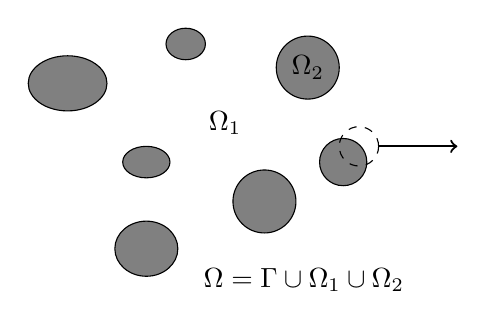
\begin{tikzpicture}
        \foreach \x/\y/\ra/\r in {
        1/3/0.2/0.25,
        2.55/2.7/0.4/0.4,
        0.5/0.4/0.35/0.4,
        2/1/0.4/0.4,
        3/1.5/0.3/0.3,
        0.5/1.5/0.2/0.3,
        -0.5/2.5/0.35/0.5}{
            \draw[fill=gray](\x,\y) ellipse(\r cm and \ra cm);
        }
        \draw[dashed](3.2,1.7)circle(0.25);
        % \draw[thick,->](3.2,1.7)++(0.1767,0.1767)--++(0.4,0.4)--++(1,0);
        \draw[thick,->](3.2,1.7)++(0.25,0)--++(1,0);
        \draw(2.55,2.7)node{$\Omega_2$};
        \draw(1.5,2)node{$\Omega_1$};
        \draw(2.5,0)node{$\Omega = \Gamma \cup \Omega_1 \cup \Omega_2$};
        % \draw(2.5,-1)node{$\Gamma = \sum_\alpha \Gamma_\alpha$};
        % \draw(2.5,-0.5)node{$\Omega_2 = \sum_\alpha \Omega_\alpha$};
    \end{tikzpicture}
    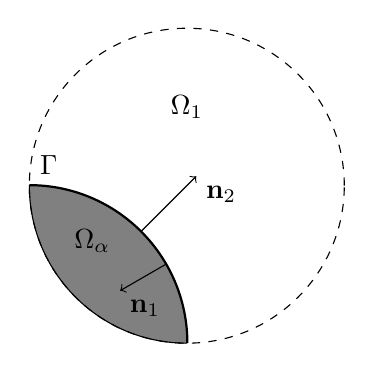
\begin{tikzpicture}%[scale = 0.9]
        \draw[very thick](0:2)arc(0:90:2)node[above right]{$\Gamma$};
        \draw[fill=gray](0:2)arc(0:90:2)arc(180:270:2);
        \draw[dashed](2,2)circle(2);
        \draw[->](1.42,1.42)--++(0.7,0.7)node[below right]{$\textbf{n}_2$};
        \draw[->](1.73,1)--++(-0.577,-0.333)node[below right]{$\textbf{n}_1$};
        \draw(2,3)node{$\Omega_1$};
        \draw(0.8,1.3)node{$\Omega_\alpha$};
    \end{tikzpicture}
    \caption{Domain definitions and scheme of the topology of dispersed two-phase flows.}
    \label{fig:Scheme}
\end{figure}
We consider a system consisting of two phases, separated by a sharp interface $\Gamma(t)$ which evolves over time. 
Each phase subdomain is denoted $\Omega_1(t)$ and $\Omega_2(t)$ for the continuous phase ($1$) and the dispersed phase ($2$) respectively (see \ref{fig:Scheme}). 
The mathematical and physical definition of $\Gamma(t)$ is by no means straightforward, therefore, the interested reader is refereed to \cite{bothe2022sharp} to have a deeper understanding of sharp interface modeling. 
The entire domain, denoted as $\Omega$, is defined as the union of $\Omega_1$, $\Omega_2$, and $\Gamma$.
To track the position of the phase indexed $k$ and the interfaces, we introduce the phase indicator function and the interface indicator function, 
\begin{align}
    \chi_k(\textbf{x},t) =  \left\{
      \begin{tabular}{cc}
        $1 \;\text{if} \;\textbf{x} \in \Omega_k(t)$\\
        $0 \;\text{if} \;\textbf{x} \notin \Omega_k(t)$
      \end{tabular}
      \right.
      \text{for $k = 1,2$},
    %   \label{eq:PIF}
    && \delta_I(\textbf{x},t) =  \left\{
      \begin{tabular}{cc}
        $1 \;\text{if} \;\textbf{x} \in \Gamma(t)$\\
        $0 \;\text{if} \;\textbf{x} \notin \Gamma(t)$
      \end{tabular}
      \right.,
      \label{eq:PIF}
\end{align}
respectively. 
For clarity, we omit the time and position arguments of $\chi_k(\textbf{x},t)$ and $\delta_I(\textbf{x},t)$ in the following sections. 

For the purpose of clarity, we only consider the specific case of the mass, momentum and energy conservation equations for a buoyant dispersed two phase flow.
Equally, we consider a constant density and viscosity in each domain as well as a constant surface tension on the interfaces.

% \subsubsection{Inside the volumes}
Within phase $k$, we note $\rho_k$ the density, $\textbf{u}_k^0$ the local velocity and $E_k^0$ the local total energy per units of mass.
All over the domain $\Omega_k(t)$ the mass, momentum and total energy obey these conservation laws :
\begin{align}
    \label{eq:dt_rho}
    \pddt \rho_k  
    + \div (
        \rho_k\textbf{u}_k^0
    )
    &= 
    0\\
    \label{eq:dt_rhou_k}
    \pddt (\rho_k\textbf{u}_k^0)  
    + \div (
        \rho_k\textbf{u}_k^0\textbf{u}_k^0
        - \bm{\sigma}_k^0 
    )
    &= 
    \rho_k \textbf{g}\\
    \label{eq:dt_rhoE_k}
    \pddt (\rho_kE_k^0)  
    + \div (
        \rho_kE_k^0\textbf{u}_k^0
        + \textbf{q}_k^0
        - \textbf{u}_k^0 \cdot \bm{\sigma}_k^0 
        )
    &= 
    \textbf{u}_k^0 \cdot \textbf{g}  \rho_k
\end{align} 
All along this work the continuous phase will be considered as Newtonian fluid thus, $\bm{\sigma}_1^0 = - p_1^0 \textbf{I} + \bm{\tau}_1^0$ where $\bm{\tau}_1^0$ is the Newtonian stress tensor with $p_1 ^0$ the local pressure and $\bm{\tau}_1^0 = \mu_1[\grad \textbf{u}_1^0+(\grad \textbf{u}_1^0)^T]$ the shear rate. 
The vector $\textbf{q}_k^0$ represent the thermal energy flux and is often model with a Fourier law : $\textbf{q}_k^0 = -\lambda \grad T_k^0$ where $T_k$ is the temperature and $\textbf{g}$ is the acceleration of gravity which will be the only body force in the present problem. 
All along this work the superscript $^0$ indicate that the variable is defied at the local or microscopic scale, in opposition to the averaged or macroscopic quantities that will be presented latter. 

% \subsubsection{On interfaces}

On the interfaces the mass, momentum and total energy balance equations reduce to the common expressions :
\begin{align}
    \label{eq:dt_rho_I}
    \textbf{u}_I = \textbf{u}_k
    &=0, \\
    \Jump{\bm{\sigma}_k^0} 
    &=
    \divI\bm\sigma^0_{I||}
    =
    \gamma\kappa\textbf{n},
    % + \gradI\sigma 
    \label{eq:surface_tension}\\
    \label{eq:dt_rhoI_uI2}
    \Jump{\textbf{u}_k^0 \cdot \bm{\sigma}_k^0}
    &=
     \gamma\kappa\textbf{n}\cdot \textbf{u}_{I}^0\\
    \label{eq:dt_rhoIe_I}
    \Jump{ \textbf{q}_k^0}
    &= 
     0
\end{align}
for the interface kinetic energy and the internal interface energy, respectively. 
Notice that this decomposition is possible only under the assumption of no mass transfer in which case $\textbf{u}_I^0=\textbf{u}_k^0$ for $k =1,2$ and a constant surface tension coefficient.



\subsection{Generic first order description of the particles}

Let us introduce the fundamental Lagrangian properties of a single particle. 
We define the mass, position of the center of mass, momentum, second moment of mass, and moment of momentum, including both the symmetric and skew-symmetric parts, of particle $\alpha$ such as, 
\begin{align}
    m_\alpha
    &= \intO{ \rho_d  },\\
    \textbf{x}_\alpha
    &= \frac{1}{m_\alpha }\intO{ \rho_d \textbf{x} },\\
    \textbf{p}_\alpha 
    &= \intO{ \rho_d \textbf{u}_d^0 },\\
    % & m_\alpha E_\alpha 
    % &= \intO{ \rho_d [e_d^0 + (u_d^0)^2/2] },\\
    \textbf{M}_\alpha 
    &= \intO{ \rho_d \textbf{rr} }, \\
    \textbf{S}_\alpha 
    &= \frac{1}{2}\intO{ \rho_d (\textbf{r}\textbf{u}_d^0+\textbf{u}_d^0\textbf{r}) },\\
    \bm\mu_\alpha 
    &= \intO{ \rho_d \textbf{r}\times\textbf{u}_d^0 },
    \label{eq:position_and_momentum_def}
\end{align}
respectively. 
We recall that $\textbf{r} = \textbf{x} - \textbf{x}_\alpha$ and that $\textbf{u}_\alpha = \textbf{p}_\alpha /m_\alpha$ is the definition of the center of mass velocity in the absence of mass transfer. 
Following the assumptions made in the preceding subsection and the generalized derivation proposed in \ref{chap:daniel2} it can be readily shown that each of these quantities satisfies the following conservation equations:
\begin{align}
    \label{eq:dt_m_alpha}
    \ddt m_\alpha
    &= 
    0\\
    \ddt {\textbf{x}_\alpha}
    &=\textbf{u}_\alpha. 
    \label{eq:dt_x_alpha}\\
    \label{eq:dt_p_alpha}
    \ddt \textbf{p}_\alpha
    &= 
    m_\alpha\textbf{g}
    +  \intS{\bm{\sigma}_f^0 \cdot \textbf{n}_d}\\
    \ddt {\textbf{M}_\alpha}
    &=2\textbf{S}_\alpha. 
    \label{eq:dt_M_alpha}
    \\
    \ddt {\textbf{S}_\alpha}
    &= \intO{ \left(
        \rho_d  \textbf{w}_d^0 \textbf{w}_d^0 
        - \bm{\sigma}_d^0
    \right) }
    - \intS{ 
        \gamma (\bm\delta - \textbf{nn})
    }
    + \frac{1}{2}\intS{ (\textbf{r}\bm{\sigma}_f^0+\bm{\sigma}_f^0\textbf{r})\cdot \textbf{n}_d} 
    \label{eq:dt_S_alpha}\\
    \ddt {\bm\mu_\alpha}
    &=
     \intS{ \textbf{r}\times(\bm{\sigma}_f^0\cdot \textbf{n}_d)} 
    \label{eq:dt_mu_alpha}
    % \label{eq:dt_E_alpha}
    % \ddt E_\alpha^\text{tot}
    % &= 
    % m_\alpha \textbf{u}_\alpha \cdot \textbf{g}
    % +\textbf{u}_\alpha \cdot \intS{\bm{\sigma}_f^0 \cdot \textbf{n}_d}
    % +\intS{\textbf{w}_f^0 \cdot \bm{\sigma}_f^0 \cdot  \textbf{n}_d} 
    % - \intS{\textbf{q}_f^0 \cdot \textbf{n}_d} 
\end{align}
This set of equations can be complemented with an equation for $M_\alpha = \frac{1}{3}\intO{\rho_d \textbf{r}\cdot \textbf{r}}$ which is obtained by taking the double contracted product of\ref{eq:dt_S_alpha} with $\bm\delta$,
it reads, 
\begin{equation}
    \frac{3}{2}\frac{d^2 M_\alpha}{dt^2}
    - \intO{ \rho_d \textbf{w}_d^0 \cdot \textbf{w}_d^0}
    = 
    - \intO{\bm\sigma_d^0:\bm\delta} 
    % - \frac{1}{3}\intS{p_f^0 \textbf{r}\cdot \textbf{n}}
    - \gamma 2 \intS{}
    % - \frac{1}{3}\intS{p_f^0 \textbf{r}\cdot \textbf{n}}
    + \intS{\textbf{r}\cdot\bm\sigma_f^0\cdot \textbf{n}}.
    \label{eq:dt_D_alpha}
\end{equation}
At this stage, the properties and evolution equations of the particles remain general and can be adapted to various types of problems. 
This general framework involves integrals of local quantities, such as $\textbf{w}_d^0$, $\bm\sigma_d^0$ \ldots and others, which are currently unknown. 
Therefore, these integral terms can be considered as closure terms since they are not yet expressed in terms of the Lagrangian unknowns, referred to as the particle's fundamental properties.
For example, in the case of solid particles, we can simplify most of these integral terms by substituting the particle's internal velocity, $\textbf{w}_d^0$ with $ \bm\omega \times \textbf{r}$. 
This solid body motion represents the simplest closure for these equations.  
Thus, for deformable fluid particles, we must find a way to reduce the degrees of freedom related to the particle shape and internal motion and develop a method to simplify the corresponding equations by finding closures for $\bm\sigma_d^0$ and $\textbf{w}_d^0$.
Consequently, in the next section, we adopt restrictive hypotheses regarding the particle shape and internal kinematics, which will allow us to partially close these equations.
% 
\subsection{Spheroidal fluid particles}

Many studies have been conducted to determine the influence of the droplets' deformation on suspension Rheology \citet{goddard1967nonlinear,lhuillier1987phenomenology,maffettone1998equation}.
Most of the authors considered the Rheology of such an emulsion for neutrally buoyant droplets in shearing flow. 
In this work we would to present a first glimps  of the form Rheology of deformable droplets or bubbles with relative motion. 
As a first step to describe the rheology we are interested in the kinematic and dynamic of a single deformable drop. 
In \ref{sec:Exemples} we study the case of 

\subsubsection*{The drop shape}

In this study we consider spheroidal particles described by a conformation tensor that we note $\textbf{C}_\alpha(t)$.  
This tensor is defined such that its eigenvalues are the dimensionless square length of the semi-axis of the spheroid minus one, such that $\textbf{C}_\alpha = (a_1^2/a^2 - 1) \textbf{pp} + (a_2^2 /a^2 - 1) (\textbf{I}-\textbf{pp})$ where $r$ is the radius of the sphere of same volume and \textbf{p} the orientation vector of the particle (see Figure \ref{fig:scheme2}).  
In this way $\textbf{C}_\alpha = 0$ when the particle is spherical and  $\textbf{C}_\alpha + \textbf{I}$ is equivalent to the Cauchy strain tensor well-defined in solid mechanics \citet{mwasame2017macroscopic}. 
In a general coordinate system the point on the surface of the spheroid verify the relation, 
\begin{equation*}
    \textbf{r}\cdot(\textbf{C}_\alpha + \textbf{I})^{-1}\cdot\textbf{r} = a^2,
\end{equation*}
\tb{is it really usefull to define this traceless matrix instead of the actual ellipse}
where $^{-1}$ is the inverse operator.  
One can verify that the second order moment of mass of the particles is related to the conformation tensor through, $\textbf{M}_\alpha = \frac{m_\alpha  a^2}{5} (\textbf{C}_\alpha + \textbf{I})$. 
The last property of the of this tensor is that it the constant volume conservation can be obtained by ensuring that $\text{det}(\textbf{C}_\alpha +\textbf{I}) = (a_1a_2^2)^2 /(a^6) = 1$. 
\begin{figure}[h!]
    \centering
    \hfill
    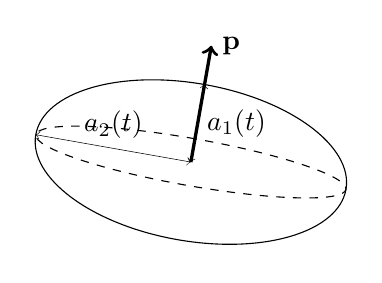
\begin{tikzpicture}[rotate=80]
        \draw(0,0) ellipse (1 cm and 2 cm);
        \draw[dashed](0,0) ellipse (0.3 cm and 2 cm);
        \draw[<->,very thin](0,0) --++ (1,0)node[midway,right]{$a_1(t)$};
        \draw[->,very thick](0,0) --++ (1.5,0)node[right]{$\textbf{p}$};
        \draw[<->,very thin](0,0) --++ (0,2)node[midway,above]{$a_2(t)$};
    \end{tikzpicture}
    \hfill
    \caption{Scheme of an  oblate spheroid oriented along the unit vector \textbf{p} with $a_1(t)$ and $a_2(t)$ the length of the semi axes of the spheroid.}
\end{figure}


\subsubsection*{The droplet internal velocity}

The internal velocity of a solid elastic particle following a homogeneous linear deformation can be described such as $\textbf{w}_2^0 = \bm\Gamma_\alpha \cdot \textbf{r}$ where we have introduced, $\bm\Gamma_\alpha$, the mean velocity gradient inside the particle, which symmetric part : $\textbf{E}_\alpha$, represents the rate of strain, and skew symmetric part : $\bm\Omega_\alpha$, represents the angular velocity. 
Even through the velocity fields $\textbf{w}_2^0 = \bm\Gamma_\alpha \cdot \textbf{r}$  can apply for liquid deforming droplet, an additional flow is present. 
Indeed, from the solution of the stokes equations we can predict the flow within a spherical isolated drop immersed in an unbounded fluid. 
Especially, we know that an solated droplet in translation exhibit internal motion known as Hill vortexes, see \ref{fig:flowlines} (b). 
For a drop immersed in an unbounded linear flow we can also derive an analytical solution such that $\textbf{w}_2^0 \sim \textbf{rrr}$, see \ref{fig:flowlines} (a). 
Therefore, the droplet's internal velocity fields is constituted with a component accounting for the complex internal motions that does not alter the shape of the drop, and another component that account for the linear deformation of the drop.  
\begin{figure*}
    \centering
    \begin{tikzpicture}
        \node (img3) at (0.6\textwidth,0) {\includegraphics[width=0.3\textwidth,angle=270]{image/Rising_def_Stokes.png}};
        \node (img2) at (0.3\textwidth,0) {\includegraphics[width=0.3\textwidth]{image/Rising_Stokes.png}};
        % \draw (0.45\textwidth,0)node{$\rightarrow$};
        % \draw (0.45\textwidth,0.4cm)node{$\bm\Gamma_\alpha\cdot \textbf{r}$};
        \node (img1) at (0.0\textwidth,0) {\includegraphics[width=0.3\textwidth]{image/Shear_Stokes.png}};
        \draw (img3.south)node{(c)};
        \draw (img2.south)node{(b)};
        \draw (img1.south)node{(a)};
    \end{tikzpicture}
    \caption{Three examples of steady state flow lines plots of an isolated droplet immersed into a viscous fluid. 
    (a) Rising sphere in uniform stokes flow (analytical solution in \ref{ap:Translating_sphere}). 
    (b) Fixed droplet in extensional flow (analytical solution in \ref{ap:Translating_sphere}).
    (c) Deformed droplet in rising motion (analytical solution of \citet{taylor1964deformation}). }
\end{figure*}
Consequently, the particle internal velocity might be written, 
\begin{equation}
    \textbf{w}_{2,i}^0(\textbf{x}_\alpha)
    = \bm\Gamma_{\alpha,ik}(t) \cdot \textbf{r}_k
    + \textbf{w}^{s}_{2,i}(t,\textbf{r})
    =\bm{\Omega}_{\alpha,ik}\cdot \textbf{r}_k
    + \textbf{E}_{\alpha,ik} \cdot \textbf{r}_k
    + \textbf{w}^{s}_{2,i}(t,\textbf{r})
\end{equation}
Where we introduced the vector $\textbf{w}^{s}_2(t,\textbf{r}) =\textbf{w}^{0}_{2,i}(t,\textbf{r})  - \bm\Gamma_{\alpha,ik}(t) \cdot \textbf{r}_k$ which represents all the internal motions that does not alter the drop's shape. 
Examples of such motions are displayed \ref{fig:flowlines}. 


From now on we consider that the internal velocity $\textbf{w}^{s}_2(t,\textbf{r})$ is not part of the particles unknown, but a function entirely determined by the particle and flow properties such that $\textbf{w}^{s}_2(t,\textbf{r}) =f_\textbf{w}(\textbf{u}_\alpha,\textbf{C}_\alpha,\bm\Gamma_\alpha,\textbf{u}_1,\bm \Gamma_1,\phi_2) $, where $\bm\Gamma_1 = \grad \textbf{u}_1$ and $\textbf{u}_1$ is the mean velocity fields evaluated at the particle position. 
As it is demonstrated in \ref{ap:Translating_sphere} the internal motion of an isolated spherical drop such as the one in \ref{eq:def_vel} might be determined theoretically from the relative motion and flow fields gradient in the limit of low Reynolds number.
We assume that such a relation exist for other regime. 
Consequently, The particle mean velocity gradient $\bm\Gamma_\alpha$ and its conformation tensor $\textbf C_\alpha$ are the only unknown of our problem. 
Therefore, we need to provide two equations, one for $\textbf{C}_\alpha$ and another for $\bm\Gamma_\alpha$. 

\subsubsection*{Kinematic and dynamic of a deformable spheroid}

The evolution of $\textbf{C}_\alpha$ and $\bm\Gamma_\alpha$ will be described by the second moment of mass and first moment of momentum equation.
Consequently, we must reformulate the terms in \ref{eq:dt_M_alpha} and \ref{eq:dt_P_alpha} in terms of $\textbf{C}_\alpha$ and $\bm\Gamma_\alpha$. 
The integrals constitutive of these moments equations can be written, 
\begin{align}
    \intO{(\textbf{rw}_2^0 )_{ij}+ (\textbf{w}_2^0 \textbf{r})_{ij}} 
    = \textbf{C}_{\alpha,ik} \cdot \bm\Gamma_{\alpha,kj}
    +  \bm\Gamma_{\alpha,ki} \cdot \textbf{C}_{\alpha,jk}
    +  \bm\Gamma_{\alpha,ij} + \bm\Gamma_{\alpha,ij}
    \\
    \intO{\rho_2 \textbf{w}_{2,i}^0\textbf{w}_{2,j}^0}
    = \frac{m_\alpha a^2}{5}[
        \bm\Gamma_{\alpha,lj}\bm\Gamma_{\alpha,ki} \textbf{C}_{\alpha,kl} 
        + \bm\Gamma_{\alpha,kj}\bm\Gamma_{\alpha,ki} 
        % + f_\textbf{ww}(\textbf{u}_\alpha,\textbf{C}_\alpha,\bm\Gamma_\alpha,\textbf{u}_1,\bm \Gamma_1,\phi_2)
        + f_\textbf{ww}(\textbf{u}_\alpha,\textbf{C}_\alpha,\bm\Gamma_\alpha,\textbf{u}_1,\bm \Gamma_1,\phi_2)
        ]
    \\
    \intO{\bm\sigma_{2,ij}^0}
    =
    % -\intO{p_2^0} \textbf{I}_{ij}
    \mu_2 v_\alpha [\bm\Gamma_{\alpha,ij} + \bm\Gamma_{\alpha,ij}
    + f_{\bm{\sigma}}(\textbf{u}_\alpha,\textbf{C}_\alpha,\bm\Gamma_\alpha,\textbf{u}_1,\bm \Gamma_1,\phi_2)]
    % + \textbf{I}_{ij}\intO{p_2^0} 
    \\
    \intS{\bm\sigma_{I,ij}^0}
    = \frac{2 \gamma v_\alpha }{a} \textbf{I}_{ij} - \frac{4 \gamma v_\alpha }{5 a} \textbf{C}_{\alpha,ij}
    +\mathcal(|\textbf{C}|^2)\\
    \intS{\textbf{r}\bm\sigma_1^0\cdot \textbf{n}_2}
    = 
    \frac{1}{2}\intS{(\textbf{r}\bm\sigma_1^0-\bm\sigma_1^0\textbf{r})\cdot \textbf{n}_2}
    + \frac{1}{2}\intS{(\textbf{r}\bm\sigma_1^0+\bm\sigma_1^0\textbf{r})\cdot \textbf{n}_2}
    % \textbf{M}(\textbf{u}_\alpha,\textbf{C}_\alpha,\bm\Gamma_\alpha,\textbf{u}_1,\bm \Gamma_1,\phi_2)
\end{align}
\tb{carry the actual decomposition with the velocity components }
\tb{mettre sous forme plus simple et expliquer l'osciallater sous forme 1d}
First, as discussed above only the deforming motion contribute to the symmetric part of the moment of momentum, we could therefore express it explicitly in terms of the particle unknown. 
Regarding the first moment of the surface tension, it has been computed analytically carrying a surface integral on the ellipsoidal surface of the droplet. 
Since, the droplets remain spheroidal under small deformation we choose to approximate $\intS{\bm\sigma_I^0}$ with its first order Taylor series in $\textbf{C}_\alpha$ without lost of generality.
Note that our expression of $\intS{\bm\sigma_I^0}$ is in agreement with \citet{lhuillier1987phenomenology} if one account for the slight difference of his definition of the deformation tensor which is half of $\textbf{C}_{\alpha}$. 
% in which our $\textbf{C}_\alpha$ is twice his, in the limit of small \textbf{C}_\alpha.
For the expression of $\intO{\rho_2 \textbf{w}_{2,i}^0\textbf{w}_{2,j}^0}$, $ \intO{\bm\sigma_{2,ij}^0}$ we had to introduce two unknown functions, $f_\textbf{ww}$, $f_{\bm{\sigma}}$, which vanish when $\textbf{w}^s_2 =0$. 
Therefore, these expressions are a sum of a function involving $\bm\Gamma_\alpha$ and an unknown part which depend on the parameters of the problem and need to be closed. 
The expression of $\intO{\rho_2 \textbf{w}_{2,i}^0\textbf{w}_{2,j}^0}$, $ \intO{\bm\sigma_{2,ij}^0}$ and $\intS{\textbf{r}\bm\sigma_1^0\cdot \textbf{n}_2}$ are very problem dependent. 
To provide a clearer example we computed these terms in \ref{ap:Translating_sphere} in the simplified scenario of an isolated droplet in a general linear flow. 

% The most common example is the expression for first moment \textbf{M}, which has been widely investigated in the pure straining situation, an example is given in \ref{ap:Translating_sphere} for spherical drop, and in \citet{raja2010inertial} for slightly deformable droplet in inertial flows. 
% It is important to notice that these functions are dependent of the relative drop-carrier fluid velocity, in such a way that the momentum and first moment of momentum are linked through the function $f_{\textbf{ww}},f_{\bm{\sigma}}$ and $\intS{\textbf{r}\bm\sigma_1^0\cdot \textbf{n}_2}$. 
% Indeed, even if it has been uniquely studied in pure linear flows, the relative motion of a particle might generate a first moment on its surface. 


At this point it wouldn't be wise trying to find an expression for each of these unknown functions in such a generality. 
Instead, we expose the unclosed set of equation of motions for spheroidal particles. 
In addition to the previously exposed equations (mass, momentum and energy equation) this system is constituted of three equations, one for $\textbf{C}_\alpha$ and two equation for the moment of momentum, the symmetric and skew-symmetric moment of momentum. 
% These read, 
\begin{align*}
    \ddt \textbf{C}_{\alpha,ij}
    = \textbf{C}_{\alpha,ik} \cdot \bm\Gamma_{\alpha,kj}
    +  \bm\Gamma_{\alpha,ki} \cdot \textbf{C}_{\alpha,jk},\\
    \frac{a^2  m_\alpha}{5} \ddt( \textbf{C}_{ik} \cdot \bm\Gamma_{\alpha,kj}
    -  \bm\Gamma_{\alpha,ki} \cdot \textbf{C}_{jk})
    =  \intS{(\textbf{r}\bm\sigma_2^0- \bm\sigma_2^0\textbf{r})\cdot \textbf{n}}\\
    \frac{m_\alpha a^2}{5}\ddt^2 \textbf{C}_\alpha
    - \frac{m_\alpha a^2}{5}[
    \bm\Gamma_{\alpha,lj}\bm\Gamma_{\alpha,ki} \textbf{C}_{\alpha,kl} + f_\textbf{ww}]
    + \mu_2 v_\alpha [(\bm \Gamma_{p,ij}+\bm \Gamma_{p,ji})
    + f_{\bm{\sigma}}]\\
    + \frac{2 \gamma v_\alpha }{a} \textbf{I}_{ij} 
    - \frac{4 \gamma v_\alpha }{5 a} (\textbf{C}_{ij} - \textbf{I}_{ij})
    = \intS{(\textbf{r}\bm\sigma_2^0+ \bm\sigma_2^0\textbf{r})\cdot \textbf{n}}
    % + \textbf{I}_{ij}\intO{p_2^0}
\end{align*}
% Where we placed the unknown function at the right hands side of these equations. 
Now, we would like to propose a more intuitive interpretation of the mass and momentum equations.
To that end, we make the problem dimensionless by introducing, 
the \textit{Capillary number} $Ca= \frac{\mu_1 U}{\gamma}$, The viscosity ratio $\lambda = \mu_2/\mu_1$, the density ratio $\zeta = \rho_2/\rho_1$ and the Reynolds number $Re = \frac{a U \rho_1}{\mu_1}$, with $U$ as the velocity scale. 
%  such that  $\bm\Gamma_\alpha'  = \frac{a}{U}\bm\Gamma$, and $\tau_a$ the timescale related to the drop shape evolution.
In the low Reynolds regime the first moment of surface traction forces will be proportional to a viscous stress (see \ref{ap:Translating_sphere}), therefore :$\intS{\textbf{r}\bm\sigma_2^0\cdot \textbf{n}} =\mu_1  \tau v_\alpha \intS{\textbf{r}\bm\sigma_2^0\cdot \textbf{n}}^*$, with $\tau$ the inverse timescale of the external solicitation.
The ratio between the external flow scale $\tau$ and the drop timescale $\tau_a$ is noted $\beta$. 
With that in mind, \ref{eq:dt_M_alpha}, \ref{eq:dt_mu_alpha} and \ref{eq:dt_S_alpha} might be written :
\begin{align}
    \beta \ddt \textbf{C}_{\alpha,ij}
    - \textbf{C}_{\alpha,ik} \cdot \bm\Gamma_{\alpha,kj}^*
    - \bm\Gamma_{\alpha,ki}^* \cdot \textbf{C}_{\alpha,jk},
    = 
    \bm\Gamma_{\alpha,ij}^*
    +  \bm\Gamma_{\alpha,ji}^*\\
    Re \zeta \beta \ddt( \textbf{C}_{\alpha,ik} \cdot \bm\Gamma_{\alpha,kj}^*
    -  \bm\Gamma_{\alpha,ki}^* \cdot \textbf{C}_{\alpha,jk}
    + \bm\Gamma_{\alpha,ji} - \bm\Gamma_{\alpha,ij})
    =  \intS{(\textbf{r}\bm\sigma_2^0- \bm\sigma_2^0\textbf{r})\cdot \textbf{n}}^*\\
    \zeta Re \frac{1}{5}  
    \left[
        \frac{1}{2}\beta^2 \ddt^2_* \textbf{C}_\alpha
        - \bm\Gamma_{\alpha,lj}^* \bm\Gamma_{\alpha,ki}^* \textbf{C}_{\alpha,kl}^* 
        - \bm\Gamma_{\alpha,kj}^* \bm\Gamma_{\alpha,ki}^* 
        - f_\textbf{ww}
    \right]\nonumber\\
    + \lambda \left[
        \beta \ddt \textbf{C}_{\alpha,ij}
        -\textbf{C}_{\alpha,ik} \cdot \bm\Gamma_{\alpha,kj}
        - \bm\Gamma_{\alpha,ki}^* \cdot \textbf{C}_{\alpha,jk},
        + f_{\bm{\sigma}}
    \right]\nonumber\\
    - \frac{1}{Ca}\left[
        \frac{4}{5} \textbf{C}_{\alpha,ij}
        +2 \textbf{I}_{ij} 
    \right]
    =
    \frac{1}{2}\intS{(\textbf{r}\bm\sigma_1^0+ \bm\sigma_1^0\textbf{r})\cdot \textbf{n}}^*
\end{align}
\tb{at this point it is not usefull to introduce the substitution in the last equaiton instead explain that it is proportional to the derivative in the limit}
The second moment of mass \ref{eq:dt_Cs}, is consistent with the equation found by \citet{goddard1967nonlinear} and \citet{lhuillier1987phenomenology}. 
Following, \citet{goddard1967nonlinear}  terminology, the left-hand side of \ref{eq:dt_Cs} is referred as the \textit{convected} derivative of $\textbf{C}^*_\alpha$. 
Therefore, the \textit{convected} derivative of $\textbf{C}_\alpha$ is equal to the rate of strain of the particle. 
The skew-symmetric part of the first moment of momentum \ref{eq:dt2_C}, it is basically the angular momentum balance of a non-spherical object. 
The right-hands side accounting for the external torque contribution. 
The symmetric part however has the form of a non-linear forced harmonic oscillatory equation for the droplet deformation. 
Indeed, the first groups of terms on the left-hand side represent the inertial contribution of the droplet internal fluid. 
It is made of a second order derivative plus non-linear terms in $\bm\Gamma_\alpha$. 
The second groups of terms is internal viscous contribution that arise directly from the definition of the stress \ref{eq:sigma_2_def}. 
It vanishes for small viscosity ration and is linear in the first derivative of $\textbf{C}_\alpha$. 
The last term on the left-hand side is the elastic response from the interface which is negligible for high capillary number $Ca \to \infty$. 
Then on right-hand side of the equation we find the first moment of surface force, $\intS{(\textbf{r}\bm\sigma_1^0+ \bm\sigma_1^0\textbf{r})\cdot \textbf{n}}^*$ which has an unknown expression at this stage. 
\ref{eq:dt2_C} might be regarded as a second order harmonic equation with non-linear contributions. 
However, the unknown function $f_\textbf{ww},\ f_{\bm{\sigma}}$ and $\intS{(\textbf{r}\bm\sigma_1^0+ \bm\sigma_1^0\textbf{r})\cdot \textbf{n}}^*$ are in general function of $\textbf{C}_\alpha$ and its higher derivatives of $\textbf{C}_\alpha$.   
Therefore, at this stage it is impossible to predict the nature of the harmonic regime followed by the droplet. 
To conclude on this matter one must find an expression for all this closure as well as determinate the impact of the non-linear terms.

We now examine the specific case studied by \citet{lamb1924hydrodynamics} where he considered no external contribution around the particle, therefore, $\intS{(\textbf{r}\bm\sigma_1^0+ \bm\sigma_1^0\textbf{r})\cdot \textbf{n}}^* = 0$.
It is found, that the amplitude of the second order harmonic mode of deformation, noted $\epsilon_2$, follows the second order partial differential equations,  
\begin{equation*}
    \ddt^2{\epsilon_2}
    + 2\lambda_2 \ddt \epsilon_2
    + \omega_2^2 \epsilon_2
     = 0,
\end{equation*}
where $\lambda_2$ and $\omega_2$ are the damping and frequency of coefficient defined as, 
\begin{align*}
    \lambda_2 = 5 \frac{\mu_2}{\rho_2a^2},
    && \omega_2 = \sqrt{8 \frac{\mu_2}{\rho_2 a^2}}.
\end{align*}
Where this equation has been obtained in the linear deformation regime for $\epsilon_2 \ll 1$. 
When multiplying \ref{eq:dt2_C} by, $\frac{10}{\zeta Re}$ we indeed find the exact same coefficient $\lambda_2$ and $\omega_2^2$ in front of, $\ddt \textbf{C}_{\alpha,ij}$ and $\textbf{C}_{\alpha,ij}$, respectively. 
In the limit of small $\textbf{C}_\alpha$, only these linear terms remain, therefore consistent with the reference work of \citet{lamb1924hydrodynamics}. 
\ref{eq:dt2_C} is somewhat more general than lamb's solution since it is expressed in an arbitrary reference frame. 
Which will prove to be useful in \ref{sec:Exemples} were we apply ensemble average on these quantities. 
However, with this equation we are able to describe only the second oscillatory mode. 
To study higher order modes one must use higher moment of momentum equations. 

In the past studies, the coupling between translational and oscillating nature of rising bubbles or droplets have been investigated \citet{lalanne2013effect}. 
For an isolated spherical droplet in translation through a stokes or potential flow we know that $
    f_\textbf{ww}
    = \frac{m_\alpha}{140 (\lambda +1)^2}
    (7 \textbf{u}_{\alpha 1} \textbf{u}_{\alpha 1} + \textbf{u}_{\alpha 1}\cdot \textbf{u}_{\alpha 1}\textbf{I})$, 
(see \ref{ap:Translating_sphere}). 
It is reasonable to guess that for a slightly spheroidal droplet in translation the expression might preserve the same form. 
Indeed, a coefficient related to $\textbf{C}_\alpha$ might appear in the expression nevertheless the overall contribution must be still proportional to $\textbf{u}_{\alpha 1} \textbf{u}_{\alpha 1}$. 
Likewise, for an inertial drops, it might be found that 
$\intS{(\textbf{r}\bm\sigma_1^0+ \bm\sigma_1^0\textbf{r})\cdot \textbf{n}}^* \sim A \textbf{u}_{\alpha 1} \textbf{u}_{\alpha 1} + B \textbf{u}_{\alpha 1} \cdot \textbf{u}_{\alpha 1}$ where $A$ and $B$ are constant. 
Indeed, the translational motion a spherical particle at slight inertia induce an overall unbalance stress on the surface of the particle generating a first moment \citet{taylor1964deformation}. 
The point is that the yet unknown closures, will help us bridge translational and drop's straining motions. 
Therefore, injecting these expressions into \ref{eq:dt2_C} would be a first step to accomplish a coupling between oscillating, or deforming motion with translating motion.
This is the subject of the last section. 
Obviously, now that we obtained a general formulation for the dynamic of the droplets' deformation, the most challenging aspect is to find expressions for closure terms. 


\subsubsection*{The particle internal energy balance.}

The surface of the particles, and internal kinetic energy can be written in this context as, 
\begin{align*}
    \beta \ddt \textbf{C}_{\alpha,ij}
    - \textbf{C}_{\alpha,ik} \cdot \bm\Gamma_{\alpha,kj}^*
    - \bm\Gamma_{\alpha,ki}^* \cdot \textbf{C}_{\alpha,jk},
    = 
    2\textbf{E}_{\alpha,ij}\\
    \intO{\rho_2 \textbf{w}_{2,i}^0\textbf{w}_{2,i}^0}
    = \frac{m_\alpha a^2}{5}[
        \bm\Gamma_{\alpha,li}\bm\Gamma_{\alpha,ki} \textbf{C}_{\alpha,kl} 
        + \bm\Gamma_{\alpha,ki}\bm\Gamma_{\alpha,ki} 
        + f_\textbf{ww}(\textbf{u}_\alpha,\textbf{C}_\alpha,\bm\Gamma_\alpha,\textbf{u}_1,\bm \Gamma_1,\phi_2)
        ]
    \\
    \intO{\bm\sigma_{2,ij}^0:\grad \textbf{u}_2^0}
    = 2 \mu_2 \intO{\textbf{e}_2^0:\textbf{e}_2^0}
    = 2\mu_2v_\alpha\left[ \textbf{E}_{\alpha,ij}\textbf{E}_{\alpha,ij}
    + f_{\textbf{e}}\right]\\
    % -\intO{p_2^0} \textbf{I}_{ij}
    \mu_2 v_\alpha [\textbf{E}_{\alpha,ij}
    + f_{\bm{\sigma}}(\textbf{u}_\alpha,\textbf{C}_\alpha,\bm\Gamma_\alpha,\textbf{u}_1,\bm \Gamma_1,\phi_2)]
    % + \textbf{I}_{ij}\intO{p_2^0} 
    \\
    s_\alpha \gamma
    = 
    \frac{3 \gamma v_\alpha }{a}\left[
        1
        + \frac{1}{20}\textbf{C}_\alpha:\textbf{C}_\alpha
    \right]
\end{align*}

\begin{equation}
    \ddt (W_\alpha + \gamma s_\alpha)
    + \intO{ \bm{\sigma}_2^0 : \grad\textbf{u}_2^0 }
    =\intS{\textbf{w}_1^0 \cdot \bm{\sigma}_1^0 \cdot \textbf{n}_2} 
\end{equation}

In conclusion, we have demonstrated how the first and second moment of momentum and mass equation can be used to describe the second mode oscillatory motion of a spheroidal drop in a Galilean reference frame. 
Therefore, the moment of momentum is a quantity of utmost importance for all kinds of particles with variable shape or volume.
This isn't limited to the momentum distribution, but all kind of properties can be described that way. 
In fact, if one wish to describe the first moment of the distribution of any local quantity $f_2^0$ and $f_I^0$ over the surface or volume of the particle, he must use the first moments' conservation equations. 
As an example, the mean concentration and distribution of surfactants on the bubbles' surface have a significant impact on the mass transfer rate between the dispersed and continuous phases.
In this case first moment of surfactant concentration could be considered here to track the evolution of the surfactant concentration and orientation over the particle surface, which would enable us to compute a better approximation of the drag force coefficient. 

% 
% \section{Re-derivation but more easy}
% \label{ap:local_basis_eq}

% All these went way to complicated. 
% So here is a more consize derivation that does keep track of the physics. 
% We describe the geometry of the particle with the second moment of mass tensor, 
% \begin{equation*}
%     M_{\alpha,ij} 
%     =\frac{m_\alpha a^2}{5} M_{\alpha,ij}^*
%     = \frac{m_\alpha a^2}{5}\left[
%         \left(
%             \frac{a_1}{a}
%         \right)^2 p_i p_j
%         + 
%         \left(
%             \frac{a_1}{a}
%         \right)^2(\delta_{ij}-  p_i p_j)
%     \right]
% \end{equation*}
% This tensor has several notable properties, the volume conservation : $a_1 a_2^2 = a^3$ which means that $\textbf{M}_\alpha^*$ has two eigenvalues linked through $M^1 = (M^2)^{-2}$ or $M^2 = (M^1)^(-1/2)$. 
% At small deformation, i.e. $M_1 - 1\ll 1$ we therefore have $M^1 = 1 - (M^1-1)/2$.
% This ultimately means that at small deformation the trace is a constant namely $M_{ij} \delta_{ij} = 3+\mathcal{O}((M^1 -1)^2)$. 




% Let's now reformulate the integral of the problem namely, 
% \begin{align}
%     \intO{(\textbf{rw}_ 2^0 )_{ij}+ (\textbf{w}_2^0 \textbf{r})_{ij}} 
%     = \textbf{M}_{\alpha,ik} \cdot \bm\Gamma_{\alpha,jk}
%         +  \bm\Gamma_{\alpha,ik} \cdot \textbf{M}_{\alpha,jk}
%     \\
%     \intO{\rho_2 \textbf{w}_{2,i}^0\textbf{w}_{2,j}^0}
%     = \bm\Gamma_{\alpha,jl}\bm\Gamma_{\alpha,ik} \textbf{M}_{\alpha,kl}  
%         +\intO{\rho_2 \textbf{w}_{2,i}^s\textbf{w}_{2,j}^s}
%     \\
%     \intO{\bm\sigma_{2,ij}^0}
%     =
%     2 \mu_2 v_\alpha \textbf{E}_{\alpha,ij}
%     - \intO{p_2^0} \textbf{I}_{ij}
%     + \mu_2 \intS{(\textbf{n}_i \textbf{w}_{2,j}^s + \textbf{n}_j \textbf{w}_{2,i}^s)}
%     \\
%     \intS{\bm\sigma_{I,ij}^0}
%     = \frac{\gamma v_\alpha }{a} \left[
%         2\textbf{I}_{ij} 
%         - \frac{4  }{5} (\textbf{M}_{\alpha,ij}^* - \textbf{I}_{\alpha,ij})
%     \right]
%     +\mathcal(O)(\textbf{C}\cdot \textbf{C})\\
%     s_\alpha 
%     = 4\pi a^2 (1+\frac{\textbf{C}:\textbf{C}}{15})
% \end{align}
% for the surface tension term is made of two terms, one corresponding to Laplace pressure and the other to the deviatoric stress. 




% The equation for the orientation, second moment of mass torque, symmetric moment of momentum and trace of the moment of momentum reads, 
% \begin{align*}
%     \ddt \textbf{pp}_{\alpha,ij}
%     = \textbf{pp}_{\alpha,ik} \cdot \bm\Omega_{\alpha,jk}
%     +  \bm\Omega_{\alpha,ik} \cdot \textbf{pp}_{\alpha,jk}\\
%     \ddt \textbf{M}_{\alpha,ij}
%     = \textbf{M}_{\alpha,ik} \cdot \bm\Gamma_{\alpha,jk}
%     +  \bm\Gamma_{\alpha,ik} \cdot \textbf{M}_{\alpha,jk}\\
%     \ddt (\textbf{I}_{\alpha,ik}\bm\omega_{\alpha,k} )
%     = 
%     \intS{(\textbf{r}\times\bm\sigma_1^0\cdot \textbf{n})_i} \\
%     \frac{1}{2}\ddt^2 \textbf{M}_{\alpha,ij}
%     -  \bm\Gamma_{\alpha,jl}\bm\Gamma_{\alpha,ik} \textbf{M}_{\alpha,kl}  
%     + 2 \mu_2 v_\alpha \textbf{E}_{\alpha,ij}
%     + \frac{\gamma v_\alpha }{a} \left[
%     2\textbf{I}_{ij} 
%     - \frac{4 \gamma v_\alpha }{5 a} (\textbf{M}_{\alpha,ij}^* - \textbf{I}_{\alpha,ij})
%     \right]\\
%     = 
%     \frac{1}{2}\intS{(\textbf{r}\bm\sigma_1^0 + \bm\sigma_1^0\textbf{r})\cdot \textbf{n}} 
%     + \intO{\rho_2 \textbf{w}_{2,i}^s\textbf{w}_{2,j}^s}
%     + \intO{p_2^0} \textbf{I}_{ij}
%     - \mu_2 \intS{(\textbf{n}_i \textbf{w}_{2,j}^s + \textbf{n}_j \textbf{w}_{2,i}^s)}\\
%     % \frac{1}{2}\ddt^2 \textbf{M}_{\alpha,mm}
%     -  \bm\Gamma_{\alpha,ml}\bm\Gamma_{\alpha,mk} \textbf{M}_{\alpha,kl}  
%     + \frac{\gamma v_\alpha }{a} 
%     % \left[
%     2\textbf{I}_{mm} 
%     % - \frac{4 }{5 } (\textbf{M}_{\alpha,mm}^* - \textbf{I}_{\alpha,mm})
%     % \right]
%     % \\
%     = 
%     \intS{\textbf{r}_m\cdot\bm\sigma_{1,mk}^0\cdot \textbf{n}_k} 
%     + \intO{\rho_2 \textbf{w}_{2,m}^s\cdot \textbf{w}_{2,m}^s}
%     + \intO{p_2^0} \textbf{I}_{mm}
% \end{align*}

% As the derivative of $M_{ij}$ in these equations actually takes in account the change of orientation of the particle it might be useful to re-derive these equations in the eigenbasis of the matrix $M_{ij}$

% To the first order in deformation the deviatoric part reads, 
% \begin{align*}
%     \frac{1}{2}\ddt^2 \textbf{M}_{\alpha,ij}
%     -   \textbf{M}_{\alpha,kl} 
%     (\bm\Gamma_{\alpha,jl}\bm\Gamma_{\alpha,ik}  
%     - \frac{1}{3}
%     \bm\Gamma_{\alpha,ml}\bm\Gamma_{\alpha,mk}  
%     \textbf{I}_{ij}
%     )
%     + 2 \mu_2 v_\alpha \textbf{E}_{\alpha,ij}
%     - \frac{\gamma v_\alpha }{a} 
%     \frac{4  }{5} (\textbf{M}_{\alpha,ij}- \textbf{I}_{ij})
%     \\
%     = 
%     \frac{1}{2}\intS{(\textbf{r}\bm\sigma_1^0 + \bm\sigma_1^0\textbf{r} - \frac{2}{3}\textbf{r}\cdot \bm\sigma_1^0 \textbf{I})\cdot \textbf{n}} 
%     + \intO{\rho_2 (\textbf{w}_{2,i}^s\textbf{w}_{2,j}^s - \frac{1}{3}\textbf{w}_{2,m}^s\textbf{w}_{2,m}^s \textbf{I}_{ij}) }
%     - \mu_2 \intS{(\textbf{n}_i \textbf{w}_{2,j}^s + \textbf{n}_j \textbf{w}_{2,i}^s)}\\
% \end{align*}
% It can be somewhat useful to extract the proportionality coefficient of each terms. 
% Denotining dimensionless qte by a $*$ we have, 
% \begin{align*}
%     \frac{\rho_2 a^2}{5 \tau^2}\left[\frac{1}{2}\ddt^2 \textbf{M}_{\alpha,ij}^*
%     -  \bm\Gamma_{\alpha,jl}^*\bm\Gamma_{\alpha,ik}^* \textbf{M}_{\alpha,kl}^*
%     \right]  
%     + \frac{2 \mu_2  }{\tau} \textbf{E}_{\alpha,ij}^*
%     + \frac{\gamma  }{a} \left[
%     2\textbf{I}_{ij} 
%     - \frac{4 }{5} (\textbf{M}_{\alpha,ij}^* - \textbf{I}_{\alpha,ij})
%     \right]\\
%     = 
%     \frac{1}{2}\intS{(\textbf{r}\bm\sigma_1^0 + \bm\sigma_1^0\textbf{r})\cdot \textbf{n}} 
%     + \intO{\rho_2 \textbf{w}_{2,i}^s\textbf{w}_{2,j}^s}
%     + \intO{p_2^0} \textbf{I}_{ij}
%     - \mu_2 \intS{(\textbf{n}_i \textbf{w}_{2,j}^s + \textbf{n}_j \textbf{w}_{2,i}^s)}\\
% \end{align*}

% The forcing terms are really problem dependent. 
% Thus, at this stage it cannot be scaled in terms of timescale. 

% In order to be more consis, we may write :
% \begin{align*}
%     \textbf{F}_{ij}(\textbf{w}^s,\bm\sigma_1^0)
%     = 
%     \frac{1}{2}\intS{(\textbf{r}\bm\sigma_1^0 + \bm\sigma_1^0\textbf{r} - \frac{2}{3}\textbf{r}\cdot \bm\sigma_1^0 \textbf{I})\cdot \textbf{n}} 
%     + \intO{\rho_2 (\textbf{w}_{2,i}^s\textbf{w}_{2,j}^s - \frac{1}{3}\textbf{w}_{2,m}^s\textbf{w}_{2,m}^s \textbf{I}_{ij}) }
%     - \mu_2 \intS{(\textbf{n}_i \textbf{w}_{2,j}^s + \textbf{n}_j \textbf{w}_{2,i}^s)}\\
% \end{align*} 
% Indicating that the forcing term is related to the exterior contribution and the external stresses. 

% \begin{align*}
%     \ddt^2 \textbf{M}_{\alpha,ij}^*
%     -2  \textbf{M}_{\alpha,kl}^* 
%     (\bm\Gamma_{\alpha,jl}^*\bm\Gamma_{\alpha,ik}^*  
%     - \frac{1}{3}
%     \bm\Gamma_{\alpha,ml}^*\bm\Gamma_{\alpha,mk}^*  
%     \textbf{I}_{ij}
%     )
%     + \frac{10 \mu_2 \tau}{ \rho_2 a^2} 2\textbf{E}_{\alpha,ij}^*
%     - 8 \frac{\tau^2 \gamma  }{\rho_2 a^3} 
%      (\textbf{M}_{\alpha,ij}^*- \textbf{I}_{ij})\\
%     = 
%     \frac{\tau^2 10}{a^2 m_\alpha}
%     \left[\textbf{F}_{\sigma_1, ij}
%     + \textbf{F}_{ww, ij}
%     + \textbf{F}_{\sigma_2, ij}\right]
% \end{align*}

% All these unclose term are really problem dependent, for now all we now is that at low Reynolds number we are in the viscous regime, besides this external flow that drives these scales. 
% Meaning that, 
% \begin{align*}
%     \intO{\rho_2 \textbf{w}_{2,i}^0\textbf{w}_{2,j}^0}
%     \sim \frac{m_\alpha a^2}{\tau_u^2} \textbf{F}_{ww}^*
%     \\
%     \mu_2 \intS{(\textbf{n}_i \textbf{w}_{2,j}^s + \textbf{n}_j \textbf{w}_{2,i}^s)}
%     \sim \frac{v_\alpha \mu_2}{\tau_u} \textbf{F}_{e}^*
%     \\
%     \intS{\bm\sigma_1^0 \textbf{rn}}
%     \sim 
%     \frac{v_\alpha \mu_1}{\tau_u} \textbf{F}_{\sigma}^*
% \end{align*} 

% \begin{align*}
%     \ddt^2 \textbf{M}_{\alpha,ij}^*
%     -2  \textbf{M}_{\alpha,kl}^* 
%     (\bm\Gamma_{\alpha,jl}^*\bm\Gamma_{\alpha,ik}^*  
%     - \frac{1}{3}
%     \bm\Gamma_{\alpha,ml}^*\bm\Gamma_{\alpha,mk}^*  
%     \textbf{I}_{ij}
%     )
%     + \frac{10 \mu_2 \tau}{ \rho_2 a^2} 2\textbf{E}_{\alpha,ij}^*
%     - 8 \frac{\tau^2 \gamma  }{\rho_2 a^3} 
%      (\textbf{M}_{\alpha,ij}^*- \textbf{I}_{ij})\\
%     = 
%     \frac{\tau^2 10 \mu_1 }{a^2 \rho_2 \tau_u}
%     \textbf{F}_{\sigma_1, ij}
%     + \frac{\tau^2 10}{\tau_u^2} \textbf{F}_{ww, ij}
%     + \frac{\tau^2 10 \mu_1 }{a^2 \rho_2 \tau_u} \textbf{F}_{\sigma_2, ij}
% \end{align*}


% \subsubsection*{Re-derivation but with dimensionless scaling}

% \begin{align}
%     \intO{(\textbf{rw}_ 2^0 )_{ij}+ (\textbf{w}_2^0 \textbf{r})_{ij}} 
%     = \textbf{M}_{\alpha,ik} \cdot \bm\Gamma_{\alpha,jk}
%         +  \bm\Gamma_{\alpha,ik} \cdot \textbf{M}_{\alpha,jk}
%     \\
%     \intO{\rho_2 \textbf{w}_{2,i}^0\textbf{w}_{2,j}^0}
%     = \bm\Gamma_{\alpha,jl}\bm\Gamma_{\alpha,ik} \textbf{M}_{\alpha,kl}  
%         +\intO{\rho_2 \textbf{w}_{2,i}^s\textbf{w}_{2,j}^s}
%     \\
%     \intO{\bm\sigma_{2,ij}^0}
%     =
%     2 \mu_2 v_\alpha \textbf{E}_{\alpha,ij}
%     - \intO{p_2^0} \textbf{I}_{ij}
%     + \mu_2 \intS{(\textbf{n}_i \textbf{w}_{2,j}^s + \textbf{n}_j \textbf{w}_{2,i}^s)}
%     \\
%     \intS{\bm\sigma_{I,ij}^0}
%     = \frac{\gamma v_\alpha }{a} \left[
%         2\textbf{I}_{ij} 
%         - \frac{4  }{5} (\textbf{M}_{\alpha,ij}^* - \textbf{I}_{\alpha,ij})
%     \right]
%     +\mathcal(O)(\textbf{C}\cdot \textbf{C})\\
%     s_\alpha 
%     = 4\pi a^2 (1+\frac{\textbf{C}:\textbf{C}}{15})
% \end{align}

% Then, 
% \begin{align*}
%     \frac{\rho_2 a^2}{5}\left[
%         \frac{1}{\tau^2}\frac{1}{2}\ddt^2 \textbf{M}_{\alpha,ij}
%     -   \frac{1}{\tau^2}\bm\Gamma_{\alpha,jl}\bm\Gamma_{\alpha,ik} \textbf{M}_{\alpha,kl}  
%     - \frac{1}{\tau_u^2} \textbf{F}_{ww}^*
%     \right]\\
%     + \mu_2  \left[
%         \frac{1}{\tau} 2\textbf{E}_{\alpha,ij}
%     + \frac{1}{\tau_u} \textbf{F}_\sigma^*
%     \right]\\
%     + \frac{\gamma  }{a} \left[
%     2\textbf{I}_{ij} 
%     - \frac{4  }{5} (\textbf{M}_{\alpha,ij}^* - \textbf{I}_{\alpha,ij})
%     \right]\\
%     = 
%     \frac{1}{2}
%     \frac{ \mu_1}{\tau_u} 
%     \textbf{F}_{\sigma_1}^*
%     % \intS{(\textbf{r}\bm\sigma_1^0 + \bm\sigma_1^0\textbf{r})\cdot \textbf{n}} 
%     % + \intO{p_2^0} \textbf{I}_{ij}
% \end{align*}

% which then, 
% \begin{align*}
%     \frac{\rho_2}{\rho_1}\frac{\rho_1 a^2}{5\mu_1\tau_u}\left[
%         \frac{\tau_u^2}{\tau^2}\frac{1}{2}\ddt^2 \textbf{M}_{\alpha,ij}
%     -   \frac{\tau_u^2}{\tau^2}\bm\Gamma_{\alpha,jl}\bm\Gamma_{\alpha,ik} \textbf{M}_{\alpha,kl}  
%     - \textbf{F}_{ww}^*
%     \right]\\
%     + \frac{\mu_2}{\mu_1}  \left[
%         \frac{\tau_u}{\tau} 2\textbf{E}_{\alpha,ij}
%     +  \textbf{F}_\sigma^*
%     \right]\\
%     + \frac{\gamma \tau_u }{a\mu_1} \left[
%     2\textbf{I}_{ij} 
%     - \frac{4  }{5} (\textbf{M}_{\alpha,ij}^* - \textbf{I}_{\alpha,ij})
%     \right]\\
%     = 
%     \frac{1}{2}
%     \textbf{F}_{\sigma_1}^*
%     % \intS{(\textbf{r}\bm\sigma_1^0 + \bm\sigma_1^0\textbf{r})\cdot \textbf{n}} 
%     % + \intO{p_2^0} \textbf{I}_{ij}
% \end{align*}

% In terms of dimensionless groups
% \begin{align*}
%     \zeta Re\left[
%         \beta^2 \frac{1}{2}\ddt^2 \textbf{M}_{\alpha,ij}
%     -   \beta^2 \bm\Gamma_{\alpha,jl}\bm\Gamma_{\alpha,ik} \textbf{M}_{\alpha,kl}  
%     - \textbf{F}_{ww}^*
%     \right]\\
%     + \lambda  \left[
%         \beta 2\textbf{E}_{\alpha,ij}
%     +  \textbf{F}_\sigma^*
%     \right]\\
%     + \frac{1}{Ca} \left[
%     2\textbf{I}_{ij} 
%     - \frac{4  }{5} (\textbf{M}_{\alpha,ij}^* - \textbf{I}_{\alpha,ij})
%     \right]\\
%     = 
%     \frac{1}{2}
%     \textbf{F}_{\sigma_1}^*
%     % \intS{(\textbf{r}\bm\sigma_1^0 + \bm\sigma_1^0\textbf{r})\cdot \textbf{n}} 
%     % + \intO{p_2^0} \textbf{I}_{ij}
% \end{align*}


% \subsubsection*{Slow flows wheer beta equal 0 }

% \textbf{Steady state equillibrium }
% \begin{align*}
%     - \zeta Re \textbf{F}_{ww}^*
%     + \lambda  \textbf{F}_\sigma^*
%     + \frac{1}{Ca} \left[
%     2\textbf{I}_{ij} 
%     - \frac{4  }{5} (\textbf{M}_{\alpha,ij}^* - \textbf{I}_{\alpha,ij})
%     \right]
%     = 
%     \frac{1}{2}
%     \textbf{F}_{\sigma_1}^*
%     % \intS{(\textbf{r}\bm\sigma_1^0 + \bm\sigma_1^0\textbf{r})\cdot \textbf{n}} 
%     % + \intO{p_2^0} \textbf{I}_{ij}
% \end{align*}

% In the last part i want to be able to neglect all the components on the left

% if the reynolds number is indeed negligible we have 

% \begin{align*}
%     + \lambda  \textbf{F}_\sigma^*
%     + \frac{1}{Ca} \left[
%     2\textbf{I}_{ij} 
%     - \frac{4  }{5} (\textbf{M}_{\alpha,ij}^* - \textbf{I}_{\alpha,ij})
%     \right]
%     = 
%     \frac{1}{2}
%     \textbf{F}_{\sigma_1}^*
%     % \intS{(\textbf{r}\bm\sigma_1^0 + \bm\sigma_1^0\textbf{r})\cdot \textbf{n}} 
%     % + \intO{p_2^0} \textbf{I}_{ij}
% \end{align*}
% which give the equillibrium of surface tension internal / external stresses
% This must be respected for almost all steady state equilibrium presented in appendix
% It is clear that if either $\lambda = 0$ or that we are looking for the fluid phase stress then the int on the left vanish. 
% And we are left with an equillibrium between surface tension and stresslet

% \tb{In this regime one might recognize Laplace law}

% \textbf{Drop in air }
% \begin{align*}
%     \zeta Re\left[
%          \frac{1}{2}\ddt^2 \textbf{M}_{\alpha,ij}
%     -    \bm\Gamma_{\alpha,jl}\bm\Gamma_{\alpha,ik} \textbf{M}_{\alpha,kl}  
%     \right]
%     +   
%         \frac{\lambda}{\beta} 2\textbf{E}_{\alpha,ij}
%     + \frac{1}{Ca\beta^2} \left[
%     2\textbf{I}_{ij} 
%     - \frac{4  }{5} (\textbf{M}_{\alpha,ij}^* - \textbf{I}_{\alpha,ij})
%     \right]\\
%     = 
%     0 
% \end{align*}
% Indeed, in this case we still consier that the surface tension is comparable with the ratio of time scale of course. 
% Besides, 
% \tb{In this regime one might recognize Lamb's equation }



\section{The local basis equation}
\label{ap:local_basis_eq}

In this appendix we give details about the derivation of the angular momentum and rate of strain equations in the local basis of the particle. 

Firstly, we consider that any second order tensor $\textbf{A}$ can be expressed in the basis formed by the unit vectors $\{\textbf{p}^0,\textbf{p}^1,\textbf{p}^2\}$, which form an orthonormal basis. 
The first vector $\textbf{p}^0$ corresponds to the vector of the particle orientation. 
The vector $\textbf{p}^1$ and $\textbf{p}^2$ are defined such that $\textbf{p}^1 \times \textbf{p} =\textbf{p}^1 \times \textbf{p}^2=\textbf{p}^2 \times \textbf{p} =0$. 
Since, the vectors $\{\textbf{p}^0,\textbf{p}^1,\textbf{p}^2\}$ form a linearly independent family, any arbitrary second order tensor  \textbf{A} can be written, 
\begin{equation}
    A_{ij}
    = 
    A^{ab}
    p_i^a
    p_j^b.
\end{equation}
The indices in superscript are used to denote the local basis tensors  components and operations, such that $A^{ab}$ corresponds to the components of \textbf{A} in the basis $\{\textbf{p}^0,\textbf{p}^1,\textbf{p}^2\}$. 
Additionally, we also used the Einstein summation convention for the indices in superscript. 
Note that the components $A^{ab}$ can be obtained from \textbf{A} applying the double contracted product,  
\begin{equation*}
    A_{ij} 
    p_i^a
    p_j^b
    = 
    A^{cd}
    p_i^c
    p_j^d
    p_i^a
    p_j^b
    = 
    A^{ab}
\end{equation*}
From there it is easy to understand that to obtain the evolution equation in the eigenbasis one has to multiply the previous set of equation with $p_i^ap_j^b$. 

Let us recall some tensor properties. 
Note that if $\bm{\Omega}$ is defined as a skew-symmetric tensor, such that, 
\begin{equation}
    \Omega_{ij} = \frac{1}{2} [A_{ij}-A_ji],
\end{equation}
then, the tensor $\bm\Omega$ written in the local basis will also be skew-symmetric, thus we have
\begin{equation}
    \Omega^{ab} = \frac{1}{2} [A^{ba}-A^{ab}]. 
\end{equation}
Indeed, using the expression of $A_{ij}$ in the local basis one may show the relation, 
\begin{equation}
    \Omega_{ij} = \frac{1}{2} [A^{ab} p^a_i p^b_j-A^{ba} p^b_j p^a_i]
    =  \frac{1}{2} [A^{ab} - A^{ba} ]p^b_j p^a_i
    =  \Omega^{ab} p^b_j p^a_i. 
\end{equation}
Therefore, by identification we deduce the former equation. 
Since the eigenvectors $\textbf{p}^0$, $\textbf{p}^1$ and  $\textbf{p}^2$ rotate according to the same angular velocity tensor $\bm\Omega$, we can write $\ddt p_i^a =\Omega_{ik} p_k^a$ for $a =0,1,2$. 
We deduce the evolution equation for the dyadic $p_i^ap_j^b$, namely,
\begin{equation*}
    \ddt(p_i^ap_j^b)
    = 
    \Omega_{ik} p_k^ap_j^b
    + \Omega_{jk} p_i^ap_k^b.
    \label{eq:orientation_pp}
\end{equation*}
This equation is the key tool that we use to reformulate \ref{eq:dt_M2}, \ref{eq:dt_S2} and \ref{eq:dt_mu2} in the particle local basis. 

\paragraph*{Local equation of the deformation:}
As described in the main text we multiply \ref{eq:dt_M2} by $p_i^ap_j^b$ and directly obtain the equaiton, 
\begin{equation*}
    \ddt M^{ab}
    = 
    M^{ac} E^{bc} 
    + E^{ac} M^{bc}. 
\end{equation*}
Note that the tensor $M^{ab}$ and $E^{ab}$ are diagonal in this basis meaning that we have, 
\begin{equation*}
    \ddt M^I
    = 
    2 M^I E^I
\end{equation*}
where $M^I$ represents the $I^{th}$ eigenvalue of the tensor $M_{ij}$. 

\paragraph*{The local equation of the rate of strain:}
We multiply, \ref{eq:dev} by $p_i^ap_j^b$, then the first term on the left-hand side of \ref{eq:dev} then reads, 
\begin{align}
    p_i^ap_j^b\ddt^2 M_{ij}
    = 
    % \ddt( p_i^ap_j^b \ddt M_{ij})
    % - \ddt (p_i^ap_j^b )\ddt M_{ij}\\
    % = 
    % \ddt( \ddt (p_i^ap_j^b M_{ij}))
    % - \ddt(   M_{ij} \ddt  p_i^ap_j^b )
    % - \ddt (p_i^ap_j^b )\ddt M_{ij}\\
    % = 
    \ddt^2 M^{ab}
    - 2 \ddt (p_i^ap_j^b) \ddt M_{ij}
    - M_{ij} \ddt^2 (p_i^ap_j^b)
    \label{eq:pp_dt2_M}
\end{align}
To get the second order derivative of $p_i^ap_j^b$ we can directly carry out the derivation, it gives, 
\begin{align*}
    \ddt\ddt(p_i^ap_j^b)
    % = 
    % \ddt (\Omega_{ik} p_k^ap_j^b)
    % + \ddt (\Omega_{jk} p_i^ap_k^b)\\
    % = 
    % \dot{\Omega}_{ik} p_k^ap_j^b
    % + \dot{\Omega}_{jk} p_i^ap_k^b
    % + (
    %     \Omega_{kl} p_l^ap_j^b
    % + \Omega_{jl} p_k^ap_l^b
    % )\Omega_{ik}
    % + (\Omega_{il} p_l^ap_k^b
    % + \Omega_{kl} p_i^ap_l^b)\Omega_{jk}\\
    = 
    \dot{\Omega}_{ik} p_k^ap_j^b
    + \dot{\Omega}_{jk} p_i^ap_k^b
    + \Omega_{ik}\Omega_{kl} p_l^ap_j^b
    + \Omega_{ik}\Omega_{jl} p_k^ap_l^b
    + \Omega_{jk}\Omega_{il} p_l^ap_k^b
    + \Omega_{jk}\Omega_{kl} p_i^ap_l^b,
\end{align*}
where we introduced the angular acceleration tensor $\dot{\Omega}_{ik} = \ddt \Omega_{ik}$. 
The third term on the right-hand side of \ref{eq:pp_dt2_M} reads, 
\begin{align*}
    M_{ij} \ddt^2 (p_i^ap_j^b)
    = M^{cb} \dot{\Omega}^{ca}
    + M^{ac} \dot{\Omega}^{cb}
    + M^{cd} \Omega^{ca}\Omega^{db}
    + M^{cd} \Omega^{ca}\Omega^{db}
    + M^{cb} \Omega^{cd}\Omega^{da} 
    + M^{ac} \Omega^{cd}\Omega^{db} 
\end{align*}
The second third term on the right-hand side of \ref{eq:pp_dt2_M} reads, 
\begin{align*}
    \ddt (p_i^ap_j^b) \ddt M_{ij}
    % = 
    % (\Omega_{ik} p_k^ap_j^b
    % + \Omega_{jk} p_i^ap_k^b)
    % (M_{il} \Gamma_{jl}
    % +  \Gamma_{il} M_{jl})\\
    = 
    + M_{cd}\Omega_{ca} \Gamma_{bd}   
    + M_{cd}\Omega_{db} \Gamma_{ac}   
    + M_{bd}\Omega_{ca} \Gamma_{cd}  
    + M_{ad}\Omega_{cb}  \Gamma_{cd} 
\end{align*}
The second term of \ref{eq:dev} multiplied by $p_i^ap_j^b$, reads, 
\begin{align*}
    p_i^a p_j^b M_{kl}( \Gamma_{jl}\Gamma_{ik} 
    - \frac{1}{3}
    \Gamma_{ml}\Gamma_{mk}  
    \delta_{ij})
    = 
    M^{cd} \Gamma^{bd}\Gamma^{ac} 
    - \frac{1}{3}
    M^{cd}\Gamma^{ed}\Gamma^{ec}  
    \delta^{ab}
\end{align*}
The of the first and second term of \ref{eq:dev} may be written in the local basis as, 
\begin{align*}
    - \frac{1}{2}(
    M^{cb} \dot{\Omega}^{ca}
    + M^{ac} \dot{\Omega}^{cb}
    + M^{cd} \Omega^{ca}\Omega^{db}
    + M^{cd} \Omega^{ca}\Omega^{db}
    + M^{cb} \Omega^{cd}\Omega^{da} 
    + M^{ac} \Omega^{cd}\Omega^{db}
)\\
    - M^{cd}\Omega^{ca} \Gamma^{bd}   
    - M^{cd}\Omega^{db} \Gamma^{ac}   
    - M^{bd}\Omega^{ca} \Gamma^{cd}  
    - M^{ad}\Omega^{cb}  \Gamma^{cd} 
    - M^{cd}( \Gamma^{bd}\Gamma^{ac} 
    - \frac{1}{3}
    \Gamma^{ed}\Gamma^{ec}  
    \delta^{ab})\\
    = 
    -\frac{1}{2}(
    M^{cb} \dot{\Omega}^{ca}
    + M^{ac} \dot{\Omega}^{cb}
    + M^{ac} \Omega^{dc} \Omega^{db}  
    + M^{bd} \Omega^{cd}  \Omega^{ca}
    + 2 M^{ac} E^{dc} \Omega^{db}  
    + 2 M^{bd} E^{cd} \Omega^{ca}
    )\\
    - M^{cd} E^{ac} E^{bd} 
    + \frac{1}{3} M^{cd}
    \Gamma^{ed}\Gamma^{ec}  
    \delta^{ab}
\end{align*}
Considering this results, we finally re-write \ref{eq:dev} in the particle eigenbasis of the particle it yields,
\begin{align*}
    \frac{1}{2}\ddt^2 M^{ab}
    -\frac{1}{2}(
        M^{cb} \dot{\Omega}^{ca}
        + M^{ac} \dot{\Omega}^{cb}
        + M^{ac} \Omega^{dc} \Omega^{db}  
        + M^{bd} \Omega^{cd}  \Omega^{ca}
        + 2 M^{ac} E^{dc} \Omega^{db}  
        + 2 M^{bd} E^{cd} \Omega^{ca}
        )\\
        - M^{cd} E^{ac} E^{bd} 
        - \frac{1}{3} M^{cd}
        \Gamma^{ed}\Gamma^{ec}  
        \delta^{ab}
    + 2 \mu_2 v_\alpha E^{ab}
    - \frac{\gamma v_\alpha }{a} 
    \frac{4  }{5} \chi^{ab}
    = F^{ab}. 
\end{align*}
This equation can be further simplified noticing that $M^{ab} = E^{ab} = 0$ for $a\neq b$, in which case we write,
\begin{align*}
    \frac{1}{2}\ddt^2 M^{ab}
    - M^{ac} \Omega^{dc} \Omega^{db}  
    - M^{cd} E^{ac} E^{bd} 
    + \frac{1}{3} M^{cd}
    \Gamma^{ed}\Gamma^{ec}  
    \delta^{ab}
    + 2 \mu_2 v_\alpha E^{ab}
    - \frac{\gamma v_\alpha }{a} 
    \frac{4  }{5} \chi^{ab}
    = F^{ab}
\end{align*}

Interestingly, when $a\neq b$ we obtain this relation, 
\begin{align*}
    -\frac{1}{2}(
        M^{cb} \dot{\Omega}^{ca}
        + M^{ac} \dot{\Omega}^{cb}
        + M^{ac} \Omega^{dc} \Omega^{db}  
        + M^{bd} \Omega^{cd}  \Omega^{ca}
        )
    = \textbf{F}^{ab}
\end{align*}
which might be considered as a constraint on the particle rotation. 

\paragraph{Local basis angular momentum equation:}
We now demonstrate how to derive the angular momentum equation in the particle eigenbasis. 
The angular momentum initially reads, 
\begin{equation*}
    \ddt (\textbf{I}_{\alpha,ik}\bm\omega_{\alpha,k} )
    = 
    \intS{(\textbf{r}\times\bm\sigma_f^0\cdot \textbf{n})_i} . 
    \label{eq:dt_mu_demo}
\end{equation*}
Firstly, the terms on the left-hand side can be written in the local basis as, 
\begin{equation*}
    I_{ik}\omega_{k}
    = 
    I^{ab} p_i^a p_k^b \omega^c p^c_k
    = 
    I^{ab}   \omega^b p_i^a. 
\end{equation*} 
Therefore, we multiply \ref{eq:dt_mu_demo} by $\textbf{p}_i^a$ which eventually leads us to the expression, 
\begin{equation*}
    \ddt (I^{ab}   \omega^b)
    = 
    + I^{ab}\omega^b p_i^a  \ddt p_i^a
    + \intS{(\textbf{r}\times\bm\sigma_f^0\cdot \textbf{n})_i} p_i^a. 
\end{equation*}
Which is the local angular momentum equation in the local reference frame of the particle, with $\omega^b$ the particle's rate of rotation in the eigenbasis. 
Nevertheless, we may simplify this equation noticing that $\ddt p_i^a = \epsilon_{ijk} \omega_j p_k^a = \epsilon_{ijk} \omega^c p_j^c p_k^a$, which gives us, 
\begin{equation*}
    \ddt (I^{ab}   \omega^b)
    = 
    I^{ab}\omega^b  \omega^c \epsilon_{ijk} p_i^a p_j^c p_k^a
    + \intS{(\textbf{r}\times\bm\sigma_f^0\cdot \textbf{n})_i} p_i^a
    = 
    % I^{ab}\omega^b  \omega^c \epsilon_{jki} p_i^a p_j^c p_k^a
    p_i^a\intS{(\textbf{r}\times\bm\sigma_f^0\cdot \textbf{n})_i}, 
\end{equation*}
where we could pass from the first to the second equality by noticing that $\epsilon_{jki} p_i^a p_j^c p_k^a = (\textbf{p}\times \textbf{p}) \cdot \textbf{p} = 0$ since the vector product of any unit tensor with itself is identically null. 
Since $I^{ab} = 0$ for $a \neq b$, we deduce that this vector equation can be reduced to these three equations for the principal values of the rotation vector, namely,
\begin{align*}
    \ddt (I^0   \omega^0)
    = 
    % I^{ab}\omega^b  \omega^c \epsilon_{jki} p_i^a p_j^c p_k^a
    p_i^0\intS{(\textbf{r}\times\bm\sigma_f^0\cdot \textbf{n})_i} \\
    \ddt (I^1   \omega^1)
    = 
    % I^{ab}\omega^b  \omega^c \epsilon_{jki} p_i^a p_j^c p_k^a
    p_i^1\intS{(\textbf{r}\times\bm\sigma_f^0\cdot \textbf{n})_i} \\
    \ddt (I^2   \omega^2)
    = 
    % I^{ab}\omega^b  \omega^c \epsilon_{jki} p_i^a p_j^c p_k^a
    p_i^2\intS{(\textbf{r}\times\bm\sigma_f^0\cdot \textbf{n})_i} 
\end{align*}
Interestingly, for solid particles, the $I^i$ are constant scalar, meaning that it is possible to simply remove these of the derivative operators. 
In our case we may reformulate the inertia tensor as, 
\begin{equation*}
    I^{ab}_\alpha
    = 
    M^{jj}_\alpha \delta^{ab}
    - M^{ab}_\alpha
    = 
    \frac{5}{m_\alpha a^2}[(\chi^{jj} + 2) \delta^{ab}
    - \chi^{ab}]
    = 
    \frac{5}{m_\alpha a^2}[2\delta^{ab} - \chi^{ab}]
    + \mathcal{O}(\chi_I^2)
\end{equation*}
where we have considered only small deformation. 
In conclusion the $I^{th}$ component of the rotation vector can be obtained using the angular momentum equation expressed in the particle eigenbasis, namely, 
\begin{align*}
    \ddt\omega^I 
    = 
    % I^{ab}\omega^b  \omega^c \epsilon_{jki} p_i^a p_j^c p_k^a
    \frac{5}{m_\alpha a^2 (2 - \chi_I)}
    \left(
    \omega^I E^I 
    +
    p_i^0\intS{(\textbf{r}\times\bm\sigma_f^0\cdot \textbf{n})_i} 
    \right). 
\end{align*}
Note that for solid particle the first term on the right-hand side vanish, as expected. 
\subsection{Oblate spheroidal fluid particles}


% \subsubsection{Shape description of the droplet}
We now consider that all particles possess an oblate spheroidal shape as represented in \ref{fig:scheme_spheroid}. 
This shape is advantageous because, for small deformations, it has been theoretically shown that droplets and bubbles tend to adopt an ellipsoidal shape. 
This holds for particles undergoing sedimentation \citep{taylor1964deformation}. 
For droplets immersed in pure linear flows it is shown that, in the limit of small deformation, the droplet shape also remain spheroidal \citep{leal2007advanced}. 
However, droplets immersed in quadratic flows do not deform as ellipsoids, as shown by \citet{nadim1991motion}. 
This implies that, for instance, in the closure problem, we must neglect the quadratic contributions from the carrier fluid. 
\begin{figure}[h!]
    \centering
    \hfill
    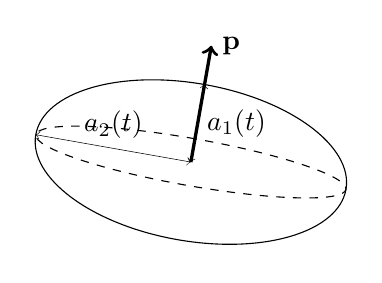
\begin{tikzpicture}[rotate=80]
        \draw(0,0) ellipse (1 cm and 2 cm);
        \draw[dashed](0,0) ellipse (0.3 cm and 2 cm);
        \draw[<->,very thin](0,0) --++ (1,0)node[midway,right]{$a_1(t)$};
        \draw[->,very thick](0,0) --++ (1.5,0)node[right]{$\textbf{p}$};
        \draw[<->,very thin](0,0) --++ (0,2)node[midway,above]{$a_2(t)$};
    \end{tikzpicture}
    \hfill
    \caption{Scheme of an  oblate spheroid oriented along the unit vector \textbf{p} with $a_f(t)$ and $a_2(t)$ the length of the semi axes of the spheroid.
    Note that when the drop is spherical we have $a_f=a_2=a$}
    \label{fig:scheme_spheroid}
\end{figure}

The shape of a particle is entirely described by an orientation vector $\textbf{p}$ and its two semi-axis, $a_1$ and $a_2$.  
By direct integration over the spheroidal particle volume in its local reference frame, i.e. the reference frame formed by $\textbf{p}$ and two other orthogonal unit vectors, it can be shown that $M_1$ and $M_2$ which are the eigenvalues of $\textbf{M}_\alpha$, read as,
\begin{align*}
    M_1 = \frac{m_\alpha a_1^2}{5},
    && M_2 = \frac{m_\alpha a_2^2}{5}.
\end{align*}
Since the particle volume remains constant over time, as given by  \ref{eq:dt_m_alpha}, we can state that $a_2^2 a_1 =a^3$, where $a$ is the radius of the equivalent spherical particle.
To measure the deviation from a spherical shape, we use the dimensionless properties $\chi_I$ and $\chi_{II}$ defined as, $\chi_I = (a_1/a)^2 - 1$ and $\chi_{II} = (a_2/a)^2 - 1$. 
With this definition, $\chi_I = 0$ when, $a_1/a =1$, in other worlds $\chi_I =\chi_{II} = 0$ when the droplet is spherical. 
Thus, $\chi_I$ will be termed the first aspect ratio of the droplet.  
Based on these definitions, the volume conservation condition \eqref{eq:dt_m_alpha} implies that $\chi_{II} = (\chi_I + 1)^{-1/2} - 1$.
% $a_2^2 a_1 =a^3 \to \chi_{II} + 1 = a /a_1$
% $\chi_I = (a_1/a)^2 - 1 \to (\chi_I +1)^{-1/2} = a/a_1$
% $a_1/a = a^2/a_2^2$
% Thus, the droplets shape is entirely determined by its orientation vector and one of its aspect ratio $\chi_I = a_1/a$ or $\chi_{II} = a_2^2/a^2$. 
Considering all these remarks we may describe the droplet shape using the dimensionless tensor, 
\begin{equation*}
    \bm\chi_\alpha
    = \frac{5}{m_\alpha a^2}\textbf{M}_\alpha - \bm\delta
    = \chi_I \textbf{pp}
        +[(\chi_I + 1)^{-1/2} - 1 ] (\bm\delta - \textbf{pp}). 
\end{equation*}
Thus, the droplet spheroidal shape is entirely characterized by two relevant parameters: the orientation vector \textbf{p} and its aspect ratio $\chi_I$.
It is interesting to notice that since $\textbf{p}$ is an eigenvector of $\textbf{M}_\alpha$ and $\bm\chi_\alpha$, $\chi_I$ and $\chi_{II}$ constitute the eigenvalues of $\bm\chi_\alpha$. 
Additionally, note that with the definition used here, $\bm\chi_\alpha +\bm\delta$ corresponds to the Cauchy green deformation tensor often employed in solid mechanics \citep{mwasame2018macroscopic}. 
The geometrical description of the surface of the droplet can also be obtained using the tensor $\bm\chi_\alpha$. 
Indeed, the distance function  $f_\alpha(\textbf{x})$, describing the particle ellipsoidal surface can be defined as \citep{nadim1996concise},  
\begin{equation*}
    f_\alpha(\textbf{x}_\alpha +\textbf{r},t) = \textbf{rr}:(\bm\chi_\alpha +\bm\delta)-a^2.  
    \label{eq:distance_function}
\end{equation*}
It is to be understood from this definition that the points $\textbf{x}$ lying on the surface of the particles respect the constraint $f_\alpha(\textbf{x},t) = 0$. 
Being able to define the droplet's surface in this way will find its use in the calculation of the surface tension stress term present in \ref{eq:dt_S_alpha}. 

% \begin{remark}{Hypothesis of small deformation :}
    
% \end{remark}
\paragraph*{Hypothesis of small deformation: }
A droplet in a pure linear flow will deform into an spheroidal shape \citet{leal2007advanced} at first order in capillary number. 
A buoyant rising droplet with the effect of small inertia will deform at the first order in $Re$ into an ellipsoid as well \citep{taylor1964deformation}.
However, as soon as the inertial effects become higher or the flow quadratic for example, the droplets' deformation is found to exhibit other shapes than spheroidal \citep{taylor1964deformation,stone1990simple}.
Therefore, in this work, we limit our study to small deformations since as soon as the droplet deformation reaches high values one might expect other shapes than ellipsoid, which is in contradiction with the initial assumption. 
Thus, to stay within our study's hypothesis we may consider only small deformation. 
This means that we neglect all the term of $\mathcal{O}(\chi_I^2)$ or $\mathcal{O}(\chi_{II}^2)$ or higher. 
In this situation notice that $\chi_{II} = (\chi_I + 1)^{-1/2} -1 \approx  - \chi_I /2$. 
Thus, the deformation tensor can be written in the simple form, 
\begin{equation}
    \bm\chi 
    = \chi_I
    \left[
        \textbf{pp} 
        - \frac{1}{2}(\bm\delta - \textbf{pp})
    \right]
    = \chi_I \frac{1}{2} \left[
        3 \textbf{pp} - \bm\delta
    \right]
    \label{eq:chi_I_small_def}
\end{equation}
Thus, the trace of $\bm\chi_\alpha$ may be written for small deformation as :  $\bm\delta:\bm\chi_\alpha  = \chi_I + 2\chi_{II} = \mathcal{O}(\chi_{I}^2)$, in other worlds for small deformation $\bm\chi_\alpha$ is purely deviatoric. 
Thus, the trace of $\bm\chi_\alpha$ is null only when considering small deformations. 
This property will be useful in the following sections.
Notice that at the next order of deformation, we have $\bm\delta:\bm\chi_\alpha  = \chi_I + 2\chi_{II} = 3 \chi_I^2 /4 +  \mathcal{O}(\chi_{I}^3)$. 

\subsection{Droplet internal velocity field}

Now that the droplet shape is properly defined we turn our attention to the description of the internal flow present within the droplets.
Indeed, the droplet internal flow $\textbf{w}_d^0$ present in the closure terms of \ref{eq:dt_S_alpha} is not part of the Lagrangian unknown, and therefore must be either directly closed or related to the Lagrangian properties which are part of the unknown of the problem.  
In \citet{lhuillier1987phenomenology} he assumes that the flow within the droplets is linear with the position. 
In our notation, this means that $\textbf{w}_d^0 = \textbf{r}\cdot \textbf{E}_\alpha(t)$ where $\textbf{E}_\alpha(t)$ corresponds to the mean rate of strain of the particle. 
In this case, $\textbf{E}_\alpha(t)$ constitutes an unknown of the particle phase which is solved in \citet{lhuillier1987phenomenology} with an equation similar to \ref{eq:dt_S_alpha}. 
For deformable solid bodies, this approach is accurate since the internal velocity field is indeed linear.
Nevertheless, as discussed in \citet{lhuillier1987phenomenology} for fluid droplets, the internal velocity field $\textbf{w}_d^0$ is far from being linear, as $\textbf{w}_d^0$ exhibits complicated fluid circulation in most of the situations, and this hypothesis is somewhat doubtful. 
Consequently, in this work, we adopt a more general approach that still accounts for the complicated internal flow present inside the particles while using a mean rate of strain tensor, $\textbf{E}_\alpha(t)$, to account for the linear deforming motions. 

It is known that an isolated droplet in creeping flow condition with relative translating motion with the carrier fluid exhibits internal motions. In this specific situation the streamlines formed by $\textbf{w}_d^0$ are known as Hill vortices, see \ref{fig:flowlines1} (b).
In this case $\textbf{w}_d^0$ has a term proportional to \textbf{rr}.  
If slightly more inertial effects are present, the initially spherical droplet deforms into an oblate spheroid \citep{taylor1964deformation}, and one might find that the internal motion of such a spheroid is close to Hill vortexes but with an oblate spheroidal shape, see \ref{fig:flowlines1} (c). 
For a drop immersed in an unbounded pure linear flow, still in stokes flow, we can derive an analytical solution for $\textbf{w}_d^0$ and find that $\textbf{w}_d^0 \sim \textbf{rrr}$ with $\textbf{r}$ the position in space relative to the center of mass of the particle, see \ref{fig:flowlines1} (a), (see \ref{chap:closure-disperse}). 
Thus, in all those cases the internal motions are more complicated than a simple linear velocity field since the internal flow is rather quadratic or cubic. 
Moreover, in all those cases the droplet's internal velocity fields are steady-state solutions.
However, for a droplet to transition from the state depicted in \ref{fig:flowlines1} (b) to the state shown in \ref{fig:flowlines1} (c) it must deform from a sphere to an oblate ellipsoid. 
Equally, a droplet immersed in a pure linear flow may experience deformation, in that case, $\textbf{w}_d^0$ and the shape of the droplet may be a function of time and capillary number \citet[chapter 7]{leal2007advanced}.
\begin{figure*}
    \centering
    \begin{tikzpicture}
        \node (img3) at (0.6\textwidth,0) {\includegraphics[width=0.3\textwidth,angle=270]{image/Rising_def_Stokes.png}};
        \node (img2) at (0.3\textwidth,0) {\includegraphics[width=0.3\textwidth]{image/Rising_Stokes.png}};
        % \draw (0.45\textwidth,0)node{$\rightarrow$};
        % \draw (0.45\textwidth,0.4cm)node{$\bm\Gamma_\alpha\cdot \textbf{r}$};
        \node (img1) at (0.0\textwidth,0) {\includegraphics[width=0.3\textwidth]{image/Shear_Stokes.png}};
        \draw (img3.south)node{(c)};
        \draw (img2.south)node{(b)};
        \draw (img1.south)node{(a)};
    \end{tikzpicture}
    \caption{Three examples of steady state flow lines plots of an isolated droplet immersed into a viscous fluid. 
    (a) Fixed droplet in extensional flow (analytical solution in \ref{chap:daniel2}).
    (b) Rising sphere in uniform stokes flow (analytical solution in \ref{chap:daniel2}). 
    (c) Deformed droplet in rising motion (analytical solution of \citet{taylor1964deformation}). }
    \label{fig:flowlines1}
\end{figure*} 

To account for this deformation in our case we assume that the \textit{transient internal velocity field} which is responsible for this deformation is homogeneous and linear with position \textbf{r}. 
Thus, the \textit{transient internal velocity field} of a particle can be modeled as $\textbf{w}_d^0 = \bm\Gamma_\alpha \cdot \textbf{r}$, where we have introduced, $\bm\Gamma_\alpha$, the mean velocity gradient inside the particle, which symmetric part: $\textbf{E}_\alpha$, represents the rate of strain, and skew-symmetric part: $\bm\Omega_\alpha$, represents the angular velocity. 
Note that the angular velocity tensor $\bm\Omega_\alpha$ is related to the angular velocity \textit{pseudo} vector $\bm\omega_\alpha$ with the relation $\bm\omega_\alpha = -\frac{1}{2}\epsilon_{ijk} (\bm\Omega_\alpha)_{jk}$. 
To summarize, we assume that the inner velocity field of the drop can be decomposed into two distinct parts. 
The first one is the steady-state component, examples are: Hill's vortices for a spherical drop in uniform linear motion, the Hill vortices-like velocity field observed for oblate spheroidal droplets in translation,  the inner velocity field of a drop in steady-state linear flows, and so on.  
The second contribution is the inner velocity fields that alter the drop's shape, this field is assumed linear with the position and homogeneous, it reads  $\bm\Gamma_\alpha\cdot \textbf{r}$. 
Adopting these definitions, the particle's internal velocity is decomposed as, 
\begin{equation}
    \textbf{w}_{d}^0[\textbf{x}_\alpha(t)+\textbf{r},t]
    = \bm\Gamma_{\alpha} \cdot \textbf{r}
    + \textbf{v}^0_{d}[\textbf{r},t]
    =\bm{\Omega}_{\alpha}\cdot \textbf{r}
    + \textbf{E}_{\alpha} \cdot \textbf{r}
    + \textbf{v}^0_{d}[\textbf{r},t]
    \label{eq:def_vel}
\end{equation}
Where we introduced the vector $\textbf{v}^0_d[\textbf{r},t] =\textbf{w}^{0}_{d}[\textbf{x}_\alpha(t)+\textbf{r},t]  - \bm\Gamma_{\alpha}[t] \cdot \textbf{r}$.
With this definition $\textbf{v}_d^0$ represents the particle's internal motion that does not contribute to the linear homogeneous deformation and angular rotation of the drop. 
Thus, $\textbf{v}_d^0$ could be one of the three velocity fields presented in \ref{fig:flowlines1}. 

Due to the consideration of mass conservation \eqref{eq:dt_m_alpha} additional properties can be noted for the tensor $\textbf{E}_\alpha$.
Indeed, at steady-state the local mass conservation inside the particle imposes that $\div \textbf{v}_d^0 = 0$. 
Thus, for a deformable droplet we obtain that $\div \textbf{u}_d^0 = \bm\Gamma_\alpha : \bm\delta = \textbf{E}_\alpha : \bm\delta =  0$.  
Also, note that to preserve the spheroidal shape of the particle we must assume that the particle's rate of strain principal direction is the same as the droplet's shape principal axis. 
In other words, $\textbf{E}_\alpha$ must have the same eigenbasis as $\textbf{M}_\alpha$. 
Making up with these two constrain leads to the expression: $\textbf{E}_\alpha = E_I \textbf{pp} + E_{II} (\bm\delta - \textbf{pp})$, where $E_I$ and $E_{II}$ are the first and second eigenvalue of $\textbf{E}_\alpha$ which are related through $E_I = - 2E_{II}$ due to the volume conservation constraint, ($\bm\delta : \textbf{E}_\alpha =0$). 


Let us now introduce the upper-convected time derivative, also known as the Oldroyd derivative, for an arbitrary Lagrangian second-order tensor $\textbf{A}$ with respect to the mean gradient $\bm\Gamma_\alpha$. 
This derivative is expressed as: 
\begin{equation}
    \overset{\triangledown  }{\textbf{A}}
    = 
    \ddt \textbf{A}
    - \textbf{A} \cdot \bm\Gamma_\alpha
    - \bm\Gamma_\alpha \cdot \textbf{A}
    \label{eq:def_upper}
\end{equation}
The physical interpretation of this operator is that it represents the time derivative of the tensor $\textbf{A}$ in a coordinate system rotating and stretching according to $\bm\Gamma_\alpha$.  
According to our assumption, the droplet shape $\textbf{M}_\alpha$ remains spheroidal under the linear transformation governed by $\bm\Gamma_\alpha$, it is self-similar. 
Additionally, recall that the field $\textbf{r}\cdot \bm\Gamma_\alpha$ accounts for the entire deformation of the droplet. 
Consequently, we deduce that:
\begin{equation}
    \overset{ \triangledown  }{\textbf{M}}_\alpha
    = 0, 
    \label{eq:def_conseq}
\end{equation}
since the shape of the droplet seen in a coordinate system that stretches and rotates with $\bm\Gamma_\alpha$ does not change \footnote{
    This expression is analogous to the definition used in rheology, which states that the upper-convected time derivative of the Finger tensor is always zero.
}.
On the other hand, substituting $\textbf{w}_d^0$ by its definition \eqref{eq:def_vel} in \ref{eq:dt_M_alpha}, gives, 
\begin{equation}
    \ddt \textbf{M}_{\alpha,ik}
    -
    \textbf{M}_{\alpha,ik} \cdot \bm\Gamma_{\alpha,kj}
    -  \bm\Gamma_{\alpha,ki} \cdot \textbf{M}_{\alpha,jk}
    =
    \intO{ 
        (\textbf{v}_{d,i}^0\textbf{r}_j
        + \textbf{r}_i\textbf{v}_{d,j}^0)
    },
\end{equation}
where we have used the Einstein indices summation convention. 
Using the definition of the upper-convected derivative given by \ref{eq:def_conseq}, leads us to the relation,
\begin{equation}
    % \overset{ \footnotesize \triangledown  }{\textbf{M}}_\alpha
    % = 
    \intO{ 
        (\textbf{v}_{d,i}^0\textbf{r}_j
        + \textbf{r}_i\textbf{v}_{d,j}^0)
    }
    =
    0.  
    \label{eq:def_v}
\end{equation}
In summary, the assumption that the droplet shape remains spheroidal and that only the linear velocity field $\textbf{r}\cdot \bm\Gamma_\alpha$ were responsible for the droplet deformation, leads us to the conclusion that $\overset{\triangledown}{\textbf{M}}_\alpha= 0$. 
Then, using the evolution equation for $\textbf{M}_\alpha$ leads us to \ref{eq:def_v}, which can be interpreted as a constraint that the field $\textbf{v}_d^0$ must satisfy. 
Thus, $\textbf{v}_d^0$ is defined by the general relation $\textbf{v}^0_d[\textbf{r},t] =\textbf{w}^{0}_{d}[\textbf{x}_\alpha(t)+\textbf{r},t]  - \bm\Gamma_{\alpha}[t] \cdot \textbf{r}$ and the constraint given by \ref{eq:def_v}. 
One can remark that this constraint is satisfied by each of the solutions represented in \ref{fig:flowlines1}.
This can be verified for the case (a) and (b) with the analytical solution provided in \ref{chap:closure-disperse}. 



% Likewise, $\textbf{v}_d^0$ is assumed not to affect the particle's angular momentum, as the kinematic description of the angular momentum is solely based on its angular velocity $\bm\Omega_\alpha$, just as $\textbf{E}_\alpha$ is assumed to be the only source of deformation. 
% The kinematic description of the angular momentum relies solely on the particle's angular velocity.
% This assumption means that the velocity decomposition has the desirable property that: $\textbf{P}_\alpha = \bm\Gamma_\alpha \cdot \textbf{M}_\alpha + \intO{\textbf{v}^0_{d,i} \textbf{r}_j} =  \bm\Gamma_\alpha \cdot \textbf{M}_\alpha $, at all times, since $\textbf{v}^0_{d,i} $ is not supposed to contribute to either the angular momentum or the symmetric part of the momentum. 
% As it will be shown this simplifies the equations of motion without entirely neglecting the internal motion.
% This means that $\textbf{v}^0_{d}$ can depend on the current shape of the particle through $\textbf{M}_\alpha$ or $\bm\chi_\alpha$ (as shown in \ref{fig:flowlines1} (c)) or its current center of mass velocity $\textbf{u}_\alpha$ (since the Magnitude of Hill vortex depends on the particle center of mass velocity), however, it must satisfy the condition $\intO{\textbf{v}^0_{d,i} \textbf{r}_j}  = 0$.



As demonstrated in \ref{chap:closure-disperse} the internal motions of an isolated spherical drop, such as the one presented in  \ref{fig:flowlines1}, are entirely determined  from $\textbf{u}_f$,$\grad\textbf{u}_f$ and $\textbf{u}_\alpha$ and the shape of the particle. 
Therefore, it is reasonable to assume that in a more general case, $\textbf{v}_d^0$ might be entirely determined by the carrier fluid and particles' properties, specifically, $\textbf{u}_\alpha$ $\textbf{M}_\alpha$, $\textbf{u}_f$ and $\grad\textbf{u}_f$. 
For non-dilute flows we might even, need to consider the volume fraction $\phi_d$ or more complicated functions.
However, this chapter will not delve into these considerations and will focus solely on dilute scenarios.
From now on we consider that the internal velocity $\textbf{v}^0_d(t,\textbf{r})$ is not part of the particle' unknown, but rather as a closure term that should be expressed in terms of $\textbf{u}_\alpha$ $\textbf{M}_\alpha$, $\textbf{u}_f$ and $\grad\textbf{u}_f$. 
Consequently, in this problem, we will explore and demonstrate how a single droplet can be exhaustively described by the parameters, $\textbf{x}_\alpha, \textbf{u}_\alpha, \bm\chi_\alpha$ and $\bm\Gamma_\alpha$, while accounting for more complex internal motion inside the droplets through different closure terms.
As we have seen $\bm\chi_\alpha$ and $\bm\Gamma_\alpha$ may also be replaced by the scalars $\chi_I$, $E_I$ and the vector \textbf{p} and $\bm\omega_\alpha$. 

\subsection{Conservation equations}

Now that the particle's shape and internal kinematics are properly defined we may simplify the moments of mass and momentum equations. 
The integrals appearing in \ref{eq:dt_M_alpha}, \ref{eq:dt_mu_alpha} and \ref{eq:dt_S_alpha} can be reformulated using the definition of $\textbf{w}_d^0$ adopted in \ref{eq:def_vel}, to find, 
\begin{align}
    \textbf{M}_\alpha 
    = \intO{ \rho_d \textbf{rr} }
    = \frac{m_\alpha a^2}{5} (\bm\chi_\alpha+\bm\delta)\\
    % \textbf{P}_\alpha = \textbf{M}_{\alpha,ik} \cdot \bm\Gamma_{\alpha,jk}\\
    \bm\mu_\alpha 
    = \intO{ \rho_d \textbf{r}\times\textbf{u}_d^0 }
    = \textbf{I}_\alpha \cdot \bm\omega_\alpha
    + \intO{ \rho_d \textbf{r}\times\textbf{v}_d^0 }
    \\
    \label{eq:S_def}
    \textbf{S}_{\alpha,ij} = \intO{(\textbf{rw}_ 2^0 )_{ij}+ (\textbf{w}_d^0 \textbf{r})_{ij}} 
    = \textbf{M}_{\alpha,ik} \cdot \bm\Gamma_{\alpha,jk}
        +  \bm\Gamma_{\alpha,ik} \cdot \textbf{M}_{\alpha,jk}
    \\
    \intO{\rho_d \textbf{v}_{d,i}^0\textbf{v}_{d,j}^0}
    = \bm\Gamma_{\alpha,jl}\bm\Gamma_{\alpha,ik} \textbf{M}_{\alpha,kl}  
    +\intO{\rho_d \textbf{v}_{d,i}^0\textbf{v}_{d,j}^0}
    \label{eq:ww_def}
    \\
    \label{eq:sigma_d_def}
    \intO{\bm\sigma_{d,ij}^0}
    =
    2 \mu_d v_\alpha \textbf{E}_{\alpha,ij}
    - \intO{p_d^0} \bm\delta_{ij}
    + \mu_d \intS{(\textbf{n}_i \textbf{v}_{d,j}^0 + \textbf{n}_j \textbf{v}_{d,i}^0)}
    \\
    \intS{\bm\sigma_{I,ij}^0}
    = \frac{\gamma v_\alpha }{a} \left[
        2\bm\delta_{ij} 
        + \frac{4  }{5} \bm\chi_{\alpha,ij}
    \right]
    +\mathcal{O}(|\bm\chi_\alpha|^2)
    % s_\alpha 
    % = 4\pi a^2 (1+\frac{\textbf{M}:\textbf{M}}{15})
\end{align}
where we have introduced the \textit{inertia moment} of the particle $\alpha$ as $\textbf{I}_\alpha = (\bm\delta : \textbf{M}_\alpha)\bm\delta - \textbf{M}_\alpha$. 
These expressions are rather straightforward since one only needs to use the definition of $\textbf{w}_d^0$ in these integrals. 
However, the surface tension stress tensor, $\intS{\bm\sigma_{I,ij}^0}$, is not so easy to obtain since it requires carrying an integral over the spheroidal surface of the particle.
Thus, the detailed calculation of the surface tension stress tensor is given in \ref{ap:surface_tension}. 
We provide the exact results as well as the Taylor expansion of this formula for small deformation. 
Notice that the spheroidal shape remains valid only for small deformations; therefore, the exact formula for $\intS{\bm\sigma_{I,ij}^0}$ considering arbitrary deformation is of limited interest. 
It is good to notice that our formula agrees with the one derived by \citet{lhuillier1987phenomenology} but with the addition of the higher order term not present in this study. 
Additionally, we can observe that two new integrals terms appeared on the right-hand side of \ref{eq:sigma_d_def}  and \ref{eq:ww_def}. 
They correspond respectively to the particle internal viscous stress and the particle internal inertial motions generated by $\textbf{v}_d^0$.
As discussed in the preceding subsection, these contributions arise from motions that are independent of particle deformation and rotation and must be treated as closure terms. 



Injecting these formulas inside \ref{eq:dt_M_alpha}, \ref{eq:dt_mu_alpha}, \ref{eq:dt_S_alpha} yields an equation for $\bm\chi_\alpha$, $\bm\omega_\alpha$ and $\textbf{E}_\alpha$, namely,
\begin{align}
    % \ddt \textbf{pp}_{\alpha,ij}
    % = \textbf{pp}_{\alpha,ik} \cdot \bm\Omega_{\alpha,jk}
    % +  \bm\Omega_{\alpha,ik} \cdot \textbf{pp}_{\alpha,jk}\\
    \overset{ \triangledown  }{\bm\chi}_\alpha
    = 
    \ddt \bm\chi_{\alpha,ij}
    -\bm\chi_{\alpha,ik} \cdot \bm\Gamma_{\alpha,jk}
    - \bm\Gamma_{\alpha,ik} \cdot \bm\chi_{\alpha,jk}
    =
    2\textbf{E}_{\alpha,ij},
    \label{eq:dt_M2}
    \\
    \ddt (\textbf{I}_{\alpha,ik}\bm\omega_{\alpha,k} )
    = 
    \intS{(\textbf{r}\times\bm\sigma_f^0\cdot \textbf{n})_i}
    - \ddt\intO{\rho_d(\textbf{r}\times \textbf{v}_d^0)_i},
    \label{eq:dt_mu2}
    \\
    \ddt \textbf{S}_{\alpha,ij}
    -  \bm\Gamma_{\alpha,jl}\bm\Gamma_{\alpha,ik} \textbf{M}_{\alpha,kl}  
    + \mu_d v_\alpha 2\textbf{E}_{\alpha,ij}
    + \frac{\gamma v_\alpha }{a} \left(
    2\bm\delta_{ij} 
    + \frac{4 }{5} \bm\chi_{\alpha,ij}
    \right) \nonumber\\
    = 
    \frac{1}{2}\intS{(\textbf{r}\bm\sigma_f^0 + \bm\sigma_f^0\textbf{r})_{ijk}\cdot \textbf{n}_k} 
    + \intO{\rho_d \textbf{v}_{d,i}^0\textbf{v}_{d,j}^0}
    + \bm\delta_{ij}\intO{p_d^0} \nonumber\\
    - \mu_d \intS{(\textbf{n}_i \textbf{v}_{d,j}^0 + \textbf{n}_j \textbf{v}_{d,i}^0)},
    \label{eq:dt_S2}
\end{align}
respectively. 
The second moment of mass \ref{eq:dt_M2}, represents the kinematic equation describing the evolution of $\bm\chi_\alpha$ due to the particle elongation and rotation. 
Note that this expression is consistent with the equation obtained by \citet{goddard1967nonlinear} if one accounts for the slightly different definitions of $\bm\chi_\alpha$ and \textbf{C} in \citet{goddard1967nonlinear}.
Following \citet{goddard1967nonlinear} the left-hand side term of \ref{eq:dt_M2} is identified as the upper-convected derivative of $\bm\chi_\alpha$, which returns the rate of strain $\textbf{E}_\alpha$. 
The equation for the skew-symmetric part of the first moment of momentum \ref{eq:dt_mu2}, is the angular momentum balance of the particle when considering the moment of inertia of a deformable particle.
Notice that in this expression the moment of inertia $\textbf{I}_\alpha$ arises naturally since its use simplifies the expression. 
The first term on the right-hand side of \ref{eq:dt_mu2} accounts for the hydrodynamic torque contribution due to the surrounding fluid.
And, the second term represents the changes of angular momentum generated by inner velocity currents. 
The symmetric part of the moment of momentum equations \ref{eq:dt_S2} is an equation for the rate of deformation, $\textbf{E}_\alpha$. 
The first two terms on the left-hand side correspond to the inertial contribution of the mean droplet rate of deformation $\textbf{E}_\alpha$. 
The third term corresponds to the contribution of the droplet's internal stress generated due to the mean drop deformation. 
The last term on the left-hand side is the contribution from the surface tension force which is the only reason why the droplet shape reaches a spherical shape equilibrium. 
These terms are directly related to either $\bm\chi_\alpha$, $\bm\omega_\alpha$ or $\textbf{E}_\alpha$, our unknowns, therefore they are gathered on the left-hand side of the equation. 
On the right-hand side of the equation, we gathered every forcing term, or closure term that is not explicitly a function of the droplet's current shape or deformation.  
The first term is the first moment of the external hydrodynamic forces, $\intS{(\textbf{r}\bm\sigma_f^0+ \bm\sigma_f^0\textbf{r})\cdot \textbf{n}}$ which is a function of the external flow properties but also of the current droplet properties. 
The second forcing term comes from the internal droplet inertia, that is the inertia related to the internal circulation of the drop. 
The third term is the mean droplet's hydrostatic pressure which is balanced mainly by the isotropic part of the surface tension contribution and the mean fluid pressure. 
The last term on the right-hand side then corresponds to the internal viscous stress generated by the relative motion of the drop with the carrier fluid. 


From \ref{eq:dt_D_alpha} we can also derive a conservation for the trace of $\bm\Gamma_\alpha$ it reads, 
\begin{equation}
    -  \bm\Gamma_{\alpha,ml}\bm\Gamma_{\alpha,mk} \textbf{M}_{\alpha,kl}  
    + \frac{\gamma v_\alpha }{a} 
    \left[
    2\bm\delta_{mm} 
    % - \frac{4 }{5 } (\textbf{M}_{\alpha,mm}^* - \textbf{I}_{\alpha,mm})
    \right]
    = 
    \intS{\textbf{r}_m\cdot\bm\sigma_{1,mk}^0\cdot \textbf{n}_k} 
    + \intO{\rho_d \textbf{v}_{d,m}^0\cdot \textbf{v}_{d,m}^0}
    + \intO{p_d^0} \bm\delta_{mm},
    \label{eq:dt_trM2}
\end{equation}
This equation, corresponds to a scalar equation describing the dynamical balance of the isotropic part of the moment of momentum of the particle. 
This equation contains the trace of every term present in \ref{eq:dt_S2} except that both viscous terms and the derivative of the trace of $\textbf{S}_\alpha$ canceled since they are traceless tensors. 
Notice that the second term on the left-hand side is the isotropic part of the surface tension forces, it corresponds to the well-known Laplace pressure. 
Additionally, on the right-hand side of \ref{eq:dt_trM2} we notice the trace of the hydrodynamic forces, which together with the particle internal pressure form the Laplace equation. 
Nevertheless, \ref{eq:dt_trM2} is more general than the classic Laplace equilibrium equation as it includes inertial effects as well as particle internal motions and deformations effects.  
Initially, \ref{eq:dt_trM2} is supposed to be used as an equation for $M_\alpha$, or more precisely the trace of $\bm\chi_\alpha$.
However, since the particle volume is assumed constant, \ref{eq:dt_trM2} can be considered as an equation for the particle mean internal pressure. 
Indeed, using that expression to cancel out the particle pressure in \ref{eq:dt_S2} gives us a novel expression that describes the deviatoric part of $\textbf{M}_\alpha$ or $\bm\chi_\alpha$.
Therefore, it corresponds to the description of the deviation from the spherical particle's shape $\bm\chi_{\alpha,ij}$. 
Indeed, injecting \ref{eq:dt_trM2,eq:dt_M2,eq:S_def} into  \ref{eq:dt_S2} one obtain, 
\begin{align}
        \frac{1}{2}\ddt^2 \bm\chi_{\alpha,ij}
        - (\bm\chi_{\alpha,kl} + \bm\delta_{kl})
        (\bm\Gamma_{\alpha,jl}\bm\Gamma_{\alpha,ik}  
        - \frac{1}{3}
        \bm\Gamma_{\alpha,ml}\bm\Gamma_{\alpha,mk}  
        \bm\delta_{ij}
        )
    &+ 
    \overset{ \triangledown  }{\bm\chi}_\alpha
    / \tau_\mu
    +
    \bm\chi_{\alpha,ij}
    / \tau_\gamma^2
    = 
    \textbf{F}_{ij}
    \label{eq:dev}
\end{align}
where,
\begin{align}
    1/\tau_\mu 
    =
    \frac{\mu_d 10}{\rho_d a^2}  
    &&
    1/\tau_\gamma^2
    = 
    \frac{\gamma 8 }{\rho_d a^3} 
\end{align}
and,
\begin{align}
    \textbf{F}_{ij}
    &= 
    \textbf{F}_{ij}^h
    +\textbf{F}_{ij}^{vv}
    + \textbf{F}_{ij}^{\sigma}\\
    \textbf{F}_{ij}^h
    &= \frac{10}{2m_\alpha a^2}\intS{(\textbf{r}\bm\sigma_f^0 + \bm\sigma_f^0\textbf{r} - \frac{2}{3}(\textbf{r}\cdot \bm\sigma_f^0) \bm\delta)\cdot \textbf{n}} \\
    \textbf{F}_{ij}^{vv}
    &= 
    \frac{10 \rho_d}{m_\alpha a^2}\intO{(\textbf{v}_{d,i}^0\textbf{v}_{d,j}^0 - \frac{1}{3}\textbf{v}_{d,m}^0\textbf{v}_{d,m}^0 \bm\delta_{ij}) }\\
    \textbf{F}_{ij}^{\sigma}
    &= - \frac{ 10 \mu_d}{m_\alpha a^2} \intS{(\textbf{n}_i \textbf{v}_{d,j}^0 + \textbf{n}_j \textbf{v}_{d,i}^0)}\nonumber
\end{align}
where we have gathered all the closures or forcing terms into the tensor $\textbf{F}_{ij}$ which has the unit [s$^{-2}$]. 
% Notice that $\textbf{E}_{\alpha,ij}$ is related to the \textit{convected} derivative of $\bm\chi_\alpha$ through \ref{eq:dt_M2}. 
One might recognize in \ref{eq:dev} a forced second-order oscillatory harmonic equation.
Indeed, the left-hand side terms correspond to the second, first and zeroth order derivative of $\bm\chi$ (i.e. $\ddt^2 \bm\chi_{\alpha,}$, $\overset{ \triangledown  }{\bm\chi}_\alpha$ and $\bm\chi_\alpha$ respectively), with the addition of the non-linear term, $ (\bm\chi_{\alpha,kl}+\bm\delta_{kl}) 
(\bm\Gamma_{\alpha,jl}\bm\Gamma_{\alpha,ik}  
- \frac{1}{3}
\bm\Gamma_{\alpha,ml}\bm\Gamma_{\alpha,mk}  
\bm\delta_{ij}
)$, while the right-hand side terms correspond to the forcing terms. 

Although oscillatory harmonic equations are typically scalar, this formulation is more general and holds for the deformation tensor. 
Notably, the coefficients $\tau_\mu$ and $\tau_\gamma$ in \ref{eq:dev} which appear in front of $\overset{ \triangledown  }{\bm\chi}_\alpha$ and $\bm\chi_\alpha$ respectively, correspond precisely to the damping ratio and the square of the natural frequency of the secondary mode of oscillation for nearly spherical droplets, as described by \citep{lamb1924hydrodynamics}. 
Indeed, in the case of freely oscillating droplets, the natural time governing the period of oscillation of droplet deformation is given by $\tau_\gamma = \sqrt{\frac{a^3\rho_d}{8 \gamma }}$ \citep{lamb1924hydrodynamics}. 
Likewise, the damping coefficient, which corresponds to the timescale over which oscillations decay, is given by  $\tau_\mu = a^2\rho_d/10 \mu_d$ \citep{lamb1924hydrodynamics}. 


To conclude, the system of equations formed by \ref{eq:dt_M2}, \ref{eq:dt_mu2} and \ref{eq:dev}, with unknown $\bm\chi_\alpha$, $\textbf{E}_\alpha$ and $\bm\omega_\alpha$, allows us to describe the deformation and the rate of deformation of a spheroidal droplet with constant volume.

\subsection{The dimensionless equations}


To enhance the physical understanding of \ref{eq:dev} we derive in the present section the dimensionless form of this equation. 
We introduce the timescale, $\tau$ which represents the droplet's natural time of deformation rate in the absence of external influences.
It is important to note that these scalings are specific to the particular scenarios described and are not applicable to general situations. 
Consequently, we consider $\tau$ as the characteristic timescale for droplet deformation, acknowledging that its exact definition remains context-dependent.
Meaning that for example, $|\ddt^2 \bm\chi_{\alpha,ij} |\sim 1/\tau^2$ and $ \overset{ \triangledown  }{\bm\chi}_\alpha \sim 1/\tau$. 
\tb{in fact that is not true $\pddt \sim 1/ \tau_u$ in podzrikidis}

Additionally, we assume that the forcing terms introduced in \ref{eq:dev} are governed by a timescale independent of the droplet's natural timescale, denoted as $\tau_u$. 
This is because the external solicitation timescale is imposed by the ``background flow'' condition and thus is quite independent of the current droplet rate of deformation. 
For example, the term $\textbf{F}_{ij}^{vv}$ representing the kinetic energy of the internal droplet velocity, is mainly driven by the relative velocity between the droplet's center of mass and the background flow. 
In fact in \ref{chap:closure-disperse} we compute this term in the situation represented in \ref{fig:flowlines1} (b) and show that $ \textbf{F}^{vv}\sim (\textbf{u}_f - \textbf{u}_p)(\textbf{u}_f - \textbf{u}_p)$. 
Thus, in this case, the timescale of the forcing term is given by $\tau_u = a /(\textbf{u}_f - \textbf{u}_p)$. 
This means that the Hill vortices velocity in \ref{fig:flowlines1} (b) are driven by the velocity scale $\textbf{u}_f - \textbf{u}_p$ and therefore the term $\textbf{F}^{vv}$ scale as $1/\tau_u^2$. 
If the ``background flow'' is not uniform but linear or represents isotropic turbulence, the principle stays the same and $\tau_u$ will be related to the background flow timescale. 
Consequently, the forcing terms can be defined proportional to the scales: 
\begin{align*}
    \textbf{F}_{ij}^h
    &= \frac{1}{2v_\alpha}\intS{(\textbf{r}\bm\sigma_f^0 + \bm\sigma_f^0\textbf{r} - \frac{2}{3}(\textbf{r}\cdot \bm\sigma_f^0) \bm\delta)\cdot \textbf{n}} 
    \sim \mu_f  /\tau_u \\
    \textbf{F}_{ij}^{vv}
    &= \frac{\rho_d}{v_\alpha}
    \intO{(\textbf{v}_{d,i}^0\textbf{v}_{d,j}^0 - \frac{1}{3}\textbf{v}_{d,m}^0\textbf{v}_{d,m}^0 \bm\delta_{ij}) }
    \sim  \rho_d a^2  /\tau_u^2 \\
    \textbf{F}_{ij}^{\sigma}
    &= - \frac{\mu_d}{v_\alpha} \intS{(\textbf{n}_i \textbf{v}_{d,j}^0 + \textbf{n}_j \textbf{v}_{d,i}^0)}
    \sim  \mu_d  /\tau_u. 
\end{align*}
Where it has been assumed that the term $\textbf{F}_{ij}^h$ scale as a viscous force. 
Re-writing \ref{eq:dt_trM2} considering these scales yields the dimensionless tensor equation, 
\begin{multline}
    \frac{\zeta Re \beta^2}{5}
    \left[
        \frac{1}{2}\ddt^2 \bm\chi_{\alpha,ij}
        -   (\bm\chi_{\alpha,kl} + \bm\delta_{kl})
        (\bm\Gamma_{\alpha,jl}\bm\Gamma_{\alpha,ik}  
        - \frac{1}{3}
        \bm\Gamma_{\alpha,ml}\bm\Gamma_{\alpha,mk}  
        \bm\delta_{ij}
        )
    \right]\\
    + \lambda \beta \overset{ \triangledown  }{\bm\chi}_\alpha
    + \frac{1}{Ca}
    \frac{4  }{5} \bm\chi_{\alpha,ij}
    = (\textbf{F}_{ij}^h )^*
    + \zeta Re (\textbf{F}_{ij}^{vv})^*
    + \lambda (\textbf{F}_{ij}^{\sigma})^* 
    \label{eq:dev_dim}
\end{multline}
where we have defined the following dimensionless groups : 
\begin{align*}
    \beta = \frac{\tau_u}{\tau},
    && \zeta = \rho_d /\rho_f,
    && \lambda = \mu_d/\mu_f,
    && Re = \frac{\rho_f a^2 }{ \mu_f \tau_u},
    && Ca = \frac{a \mu_f}{\gamma \tau_u}. 
\end{align*}
The superscript $^*$ indicates that the argument is made dimensionless. 
Each of these dimensionless numbers has a distinct physical signification. 
Let us start with $\beta$, this number compares the typical timescale of the external contribution with the natural timescale of the droplets' deformation.
$\zeta$ is the ratio of the carrier fluid density to the droplet density. 
$\lambda$ is the ratio of the carrier fluid viscosity to the droplet viscosity. 
The number $Re$ compares the viscous forces to inertial forces. 
And $Ca$ is the ratio of the capillary forces compared to the viscous forces. 
Thus, on the left-hand side of \ref{eq:dev_dim} we identify the inertial terms; (the terms factor of $Re$), the viscous terms (i.e. the terms factor of $\lambda$) and the surface tension or capillary contribution which are factor of $1/Ca$. 
The same comments can be made regarding the forcing terms on the right-hand side. 


We will now explore specific regimes where this equation simplifies. To provide a clearer physical understanding, we consider four different scenarios: the low Reynolds number regime, the quasi-steady regime, the bubbly flow regime, and the free-oscillating droplet regime. 


\subsubsection{Free oscillating droplets}

As a first example let us consider a freely oscillating droplet, meaning that we neglect the carrier fluid property. 
This example applies well to viscous droplets in air where the influence of the carrier fluid on the droplet can be completely neglected, meaning that all the forcing terms on the right-hand side of \ref{eq:dev_dim} can be ignored.\footnote{
    Note that even $\textbf{F}^{vv}$ can be neglected since it is the external forcing that induces an internal velocity through the droplet interface motion, hence in the absence of external forcing  $\textbf{F}^{vv}=0$.  
} 
Thus, \ref{eq:dev_dim} reduce to, 
\begin{multline}
    \frac{\zeta Re \beta^2}{5}
    \left[
        \frac{1}{2}\ddt^2 \bm\chi_{\alpha,ij}
        -  ( \bm\chi_{\alpha,kl} +\bm\delta_{kl})
        (\bm\Gamma_{\alpha,jl}\bm\Gamma_{\alpha,ik}  
        - \frac{1}{3}
        \bm\Gamma_{\alpha,ml}\bm\Gamma_{\alpha,mk}  
        \bm\delta_{ij}
        )
    \right]
    + \lambda \beta \overset{ \triangledown  }{\bm\chi}_\alpha
    + \frac{1}{Ca}
    \frac{4  }{5} \bm\chi_{\alpha,ij}
    =
    0.
\end{multline}
In this regime, the droplet shape follows a non-linear homogeneous partial differential tensorial equation. 
As no forcing terms are present in this equation, we can predict that in the steady state $\bm\chi_\alpha = 0$ meaning that the droplet shape will eventually relax into a spherical shape in this regime.
This holds under the condition that $\lambda$ remains finite.   
% In the following we show that, upon linearizing this equation, we recover the second-order free-oscillatory harmonic equations introduced by \citet{lamb1924hydrodynamics}. 

\subsubsection{Low Reynolds number or viscous dominated regime}

Now, let us assume that the relative motion between the droplets and the carrier phase is rather viscous such that $Re \ll 1$.
In this situation \ref{eq:dev_dim} reduces to, 
\begin{equation*}
    % \frac{\zeta Re \beta^2}{5}
    % \left[
    %     \frac{1}{2}\ddt^2 \bm\chi_{\alpha,ij}
    %     -   \textbf{M}_{\alpha,kl} 
    %     (\bm\Gamma_{\alpha,jl}\bm\Gamma_{\alpha,ik}  
    %     - \frac{1}{3}
    %     \bm\Gamma_{\alpha,ml}\bm\Gamma_{\alpha,mk}  
    %     \bm\delta_{ij}
    %     )
    % \right]\\
    \lambda \beta \overset{ \triangledown  }{\bm\chi}_\alpha
    + \frac{1}{Ca}
    \frac{4  }{5} \bm\chi_{\alpha,ij}
    = (\textbf{F}_{ij}^h)^* 
    % + \zeta Re \textbf{F}_{ij}^{vv}
    + \lambda (\textbf{F}_{ij}^{\sigma})^*
    \label{eq:stokes_shape}
\end{equation*}
We can observe that in this regime the shape of the particle is governed by a balance of viscous stress due to the rate of current deformation (first term), the surface tension force (second term), the external hydrodynamic contribution (first term on the right-hand side), and finally the particle's internal viscous stresses generated due to the internal re-circulation (second term on the right-hand side). 
This situation is typically experienced by neutrally buoyant droplets immersed in a shear flow at low $Re$. 
For example in \citet[Chapter 7]{leal2007advanced} they derive the evolution equation for a deformable droplet in a pure linear flow, in this case, this balance should hold. 

\subsubsection{Quasi-steady state regime}

% In certain situations the natural times related to the droplet rate of deformation, $\tau$, is greater than the timescale of the external flow $\tau_u$ which is generally much smaller. 
Let us consider the situation of rising buoyant droplets or bubbles. 
In that case, the external contributions are all proportional to the only relative motion present in homogeneous rising flows which is the relative phase velocity $\textbf{u}_p-\textbf{u}_f$ (or the square of that in inertial regime).
When the droplets reach their terminal rising velocity it is clear that $\tau_u \sim a / \textbf{u}_p-\textbf{u}_f $.
On the other hand, the natural times related to the droplet rate of deformation might be given either by $1 / \tau \sim \sqrt{\frac{ \gamma }{a^3\rho_d}}$ or $\sim  \mu_d  /(a^2\rho_d)$. 
Therefore, the Quasi-steady state assumption, $\beta \ll 1$ requires, 
\begin{equation}
  1/\beta^2 =  \frac{a\rho_d |\textbf{u}_p-\textbf{u}_f|^2}{\gamma } = \zeta We \gg 1 
\end{equation}
Or, 
\begin{equation}
    1/\beta = (a\rho_d|\textbf{u}_p-\textbf{u}_f|)/(\mu_d ) = \frac{\zeta Re }{\lambda} \gg 1
\end{equation}

Thus, in this case, $\beta \ll 1$ and we can neglect the transient effects arising due to the droplets' deformation, which yields, 
\begin{equation}
    % \frac{\zeta Re \beta^2}{5}
    % \left[
    %     \frac{1}{2}\ddt^2 \bm\chi_{\alpha,ij}
    %     -   \textbf{M}_{\alpha,kl} 
    %     (\bm\Gamma_{\alpha,jl}\bm\Gamma_{\alpha,ik}  
    %     - \frac{1}{3}
    %     \bm\Gamma_{\alpha,ml}\bm\Gamma_{\alpha,mk}  
    %     \bm\delta_{ij}
    %     )
    % \right]\\
    % \lambda \beta 2 \textbf{E}_{\alpha,ij}
    \frac{1}{Ca}
    \frac{4  }{5} \bm\chi_{\alpha,ij}
    = (\textbf{F}_{ij}^h)^*
    + \zeta Re (\textbf{F}_{ij}^{vv})^*
    + \lambda (\textbf{F}_{ij}^{\sigma})^*
    \label{eq:steady}
\end{equation}
Consequently, in the quasi-steady-state regime, the droplet deformation is given explicitly by the sum of: the external hydrodynamic contribution; the inertial due to internal particle re-circulation; and the particle internal stresses due to this internal motion. 
Notice that in \citet{taylor1964deformation} they compute the shape of a steady state rising droplet analytically and consider low but finite inertial effects. 
In this case \ref{eq:steady} typically governs the shape balance.
 

\subsubsection{Bubbly flow regime}
Finally, for bubbly flows where the density and viscosity of the bubbles are negligible compared to those of the carrier fluid, we have $\zeta \ll 1$ and $\lambda \ll 0$. 
In this particular situation, the shape equation simplifies significantly to:
\begin{equation}
    % \frac{\zeta Re \beta^2}{5}
    % \left[
    %     \frac{1}{2}\ddt^2 \bm\chi_{\alpha,ij}
    %     -   \textbf{M}_{\alpha,kl} 
    %     (\bm\Gamma_{\alpha,jl}\bm\Gamma_{\alpha,ik}  
    %     - \frac{1}{3}
    %     \bm\Gamma_{\alpha,ml}\bm\Gamma_{\alpha,mk}  
    %     \bm\delta_{ij}
    %     )
    % \right]\\
    % \lambda \beta 2 \textbf{E}_{\alpha,ij}
    \frac{1}{Ca}
    \frac{4  }{5} \bm\chi_{\alpha,ij}
    = (\textbf{F}_{ij}^h)^*. 
    \label{eq:bubbles}
\end{equation}
This implies that the shape of a bubble is entirely determined by the external fluid solicitation. 
The absence of both $\textbf{E}_\alpha$ and the derivative of $\bm\chi_\alpha$ indicates that bubbles adjust their shape instantaneously to the carrier fluid’s forces.

However, it is known that bubbles in water can still exhibit oscillations due to the added mass effect. 
This might seem contradictory to \ref{eq:bubbles} as no second-order derivatives of $\bm\chi_\alpha$ are present in this equation. 
However, the term $\textbf{F}_{ij}^h$ can be proportional to $\ddt^2 \bm\chi_\alpha$ with the proportionality constant being the added mass coefficient, which is related to the first moment of the hydrodynamic forces. 
In that case, the natural oscillation frequency of the bubbles will be related to added mass effects. 

As stated earlier, the spheroidal shape of a particle can be described uniquely using the scalars $\chi_I$ and $E_I$ since the other components of $\bm\chi_\alpha$ and $\textbf{E}_\alpha$ might be entirely deduced from $\chi_I$ and $E_I$, and the orientation vector \textbf{p}. 
Therefore, progress can be made to reduce this system of tensor equations to one equation for \textbf{p}, $\bm\omega_\alpha$ and two scalars equations, one for $\chi_I$ and another for $E_I$. 
This is the purpose of the next subsection. 


\subsection{Local reference frame equations}

In order to derive equations for the scalars $\chi_I$ and $E_I$ we demonstrate here that we need to express \ref{eq:dt_M2} and \ref{eq:dev} in they principal basis, i.e. the basis formed by the eigenvector of $\bm\chi_\alpha$ and $\textbf{E}_\alpha$. 
Since we are not interested in all eigenvalues of $\bm\chi_\alpha$ and $\textbf{E}_\alpha$ but rather only on $\chi_I$ and $E_I$, it is sufficient to project the equations onto the first eigenvector $\textbf{p}$. 

\subsubsection{Preliminaries and orientation equation}
We first introduce the relation,
\begin{equation}
    \bm\chi_{\alpha,ij} \textbf{p}_i\textbf{p}_j
    = 
    (
        \chi_I \textbf{p}_i\textbf{p}_j
        + \chi_{II} (\bm\delta_{ij} - \textbf{p}_i\textbf{p}_j)
    ) \textbf{p}_i\textbf{p}_j
    = \chi_I.
    \label{eq:chi_I_def}
\end{equation} 
This relation simply states that the projection of $\bm\chi_\alpha$ on its first eigenvector $\textbf{p}$, returns (by definition) its first eigenvalue $\chi_I$. 
Likewise, we might show that, 
\begin{equation}
    \textbf{E}_{\alpha,ij} \textbf{p}_i\textbf{p}_j
    = 
    (
        E_I \textbf{p}_i\textbf{p}_j
        + E_{II} (\bm\delta_{ij} - \textbf{p}_i\textbf{p}_j)
    ) \textbf{p}_i\textbf{p}_j
    = E_I.
    \label{eq:E_I_def}
\end{equation} 
Notice that this equation requires that the main axis of deformation occurs in the same direction as the current state of deformation, that is in the direction of $\textbf{p}$. 
As mentioned earlier this assumption is made here, since to preserve the droplet spheroidal shape the deformation must occur along the axis of deformation. 
One might deduce that to derive an equation for $\chi_I$ one just need to multiply \ref{eq:dt_M2} by $\textbf{p}_i \textbf{p}_j$, likewise to obtain an equation for $E_I$ one needs to multiply \ref{eq:dev} by $\textbf{p}_i \textbf{p}_j$. 
Nevertheless, notice that this will make appear the derivative of $\textbf{p}_i \textbf{p}_j$ in the resulting equations, introducing the need of a transport equation for this tensor. 

Therefore, let us focus on the derivation of an equation for the tensor  $\textbf{p}_i \textbf{p}_j$. 
This transport equation is straightforward to obtain if one first notices that due to purely kinematics constraints, any unit vector \textbf{p} follows the kinetic relation $\ddt \textbf{p} = \bm\Omega_\alpha \cdot \textbf{p}$.
Indeed, the angular velocity of \textbf{p} corresponds, by definition, to the particle's angular velocity. 
Taking the time derivative of $\textbf{pp}$ and using the chain rule directly yields the relation, 
\begin{equation}
    \ddt (\textbf{pp})_{ij}
    = 
    (\textbf{pp})_{ik}\cdot\bm\Omega_{\alpha,jk}. 
    +\bm\Omega_{\alpha,ik}\cdot (\textbf{pp})_{jk}
    \label{eq:dt_pp}
\end{equation}
Notice that this equation is extensively used in fiber media theory to predict the evolution of fiber orientation in a medium. 
% This equation constitutes the theoretical ground from which all Folgar-Tukers-like models are derived. 
% This will be discussed in the next section.

\subsubsection{Local reference frame kinematic equation}

Now that the basic relations are derived let us focus on the derivation of the equation for $\chi_I$. 
Multiplying \ref{eq:dt_M2} by $(\textbf{pp})_{ij}$ and using \ref{eq:chi_I_def},\ref{eq:E_I_def} and  \ref{eq:dt_pp} gives, 
\begin{equation}
    \ddt \chi_I
    = 
    \bm\chi_{\alpha,ij} [(\textbf{pp})_{ik}\cdot\bm\Omega_{\alpha,jk}. 
    +\bm\Omega_{\alpha,ik}\cdot (\textbf{pp})_{jk}]
    + (\textbf{pp})_{ij}(\bm\chi_{\alpha,ik} \cdot \bm\Gamma_{\alpha,jk}
    + \bm\Gamma_{\alpha,ik} \cdot \bm\chi_{\alpha,jk}
    + 2\textbf{E}_{\alpha,ij})
    \label{eq:step_one}
\end{equation}
The product $\bm\chi_{ij} (\textbf{pp})_{ik}$ and $(\textbf{pp})_{ij}\bm\chi_{\alpha,ik}$ both gives, 
\begin{equation*}
    \bm\chi_{ij} (\textbf{pp})_{ik}
    =
    (\textbf{pp})_{ij}\bm\chi_{\alpha,ik}
    = 
    \chi_I (\textbf{pp})_{jk}
\end{equation*}
and so on for $\bm\chi_{ij} (\textbf{pp})_{jk}$ and $(\textbf{pp})_{ij} \bm\chi_{\alpha,jk}$. 
Thus, the right-hand side of \ref{eq:step_one} may be written as, 
\begin{equation}
    \ddt \chi_I
    = 
    \chi_I [(\textbf{pp})_{jk}:(\bm\Omega_{\alpha,jk} + \bm\Gamma_{\alpha,jk}). 
    +(\bm\Omega_{\alpha,ik} + \bm\Gamma_{\alpha,ik}) :(\textbf{pp})_{ik}]
    + 2E_I
    \label{eq:step_two}
\end{equation}
One might directly notice that the skew-symmetric part of $\bm\Gamma_\alpha$ and the tensor $\bm\Omega_\alpha$ vanish due to the double contracted product with the symmetric tensor $\textbf{pp}$. 
This finally gives 
\begin{equation}
    \ddt \chi_I
    = 
    2(\chi_I +1)E_I. 
    \label{eq:dt_chi_I}
\end{equation}
This equation simply states that the derivative of the deformation corresponds to the rate of strain in that same direction time the current deformation plus one.  
Rearranging this equation one can equally show that $2E_I = \ddt (\ln(\chi_I+1))$ which for small deformations gives,
\begin{equation}
    2E_I =  \ddt \chi_I + \mathcal{O}(\chi_I^2). 
    \label{eq:small_def}
\end{equation}
The absence of $\bm\Omega_\alpha$ indicates that in the local basis of the particle, the rotation of the latter does not impact the kinematic relation between the deformation $\chi_I$ and the rate of deformation $E_I$.
This is easily understandable as it is a kinematic relation. 
In contrast, the particle's rotation plays a significant role in the particle's dynamical balance equations.


\subsubsection{Local reference frame dynamic equations}
% \subsubsection{The local reference frame rate of strain equations}

Now we apply the same reasoning on the rate of strain conservation \eqref{eq:dt_S2} and angular momentum conservation \eqref{eq:dt_mu_alpha},
by multiplying each terms on the left-hand side of \ref{eq:dt_S2} and \ref{eq:dt_mu_alpha} by $(\textbf{pp})_{ij}$. 
As the mathematical derivation is more lengthily, the details are presented in \ref{ap:local_basis_eq}. 
Note that in \ref{ap:local_basis_eq} we demonstrate how to project an equation or tensor on its $3$ eigenvectors, not only the first one ($\textbf{p}$). 
To accomplish such a task we have to introduce the \textit{local basis notations}. 
Let us consider the local basis $\{\textbf{p}^0, \textbf{p}^1, \textbf{p}^2\}$ which constitutes an orthonormal eigenbasis of both the tensors $\bm\chi_\alpha$ and $\textbf{E}_\alpha$. 
It must be understood here that $\textbf{p}^0 = \textbf{p}$. 
Then, any second-order tensor $A_{ij}$ can be written in the form, 
\begin{equation*}
    (\textbf{A})_{ij}
    = 
    \sum_{a,b =1}^3
    (A^{ab} \textbf{p}^a\textbf{p}^b)_{ij}
    = 
    \sum_{a,b =1}^3
    A^{ab} p_i^ap_j^b,
\end{equation*}
where $A^{ab}$ are the scalar components of the tensor \textbf{A} in the local basis  $\{\textbf{p}^0, \textbf{p}^1, \textbf{p}^2\}$. 
If $\{\textbf{p}^0, \textbf{p}^1, \textbf{p}^2\}$ constitutes an eigenbasis of the tensor \textbf{A} then the off diagonal components $A^{ab}$ with $a\neq b$ all vanish. 
Thus, one is left with the formula, 
\begin{equation*}
    A_{ij}
    = 
    \sum_{a =1}^3
    A^{aa} p_i^ap_j^a. 
\end{equation*}
Where the $A^{aa}$ are the eigenvalues of the tensor \textbf{A}. 
Particularly, since $\{\textbf{p}^0, \textbf{p}^1, \textbf{p}^2\}$ is the eigenbasis of $\bm\chi_\alpha$ and $\textbf{E}_\alpha$ we can write, 
\begin{align*}
    (\bm\chi_\alpha)_{ij}
    =
    \sum_{a =1}^3
    (\chi^{aa} \textbf{p}^a\textbf{p}^a)_{ij}. 
    =
    \chi_I  p_i^0p_j^0
    + \chi_{II}  p_i^1p_j^1
    + \chi_{II}  p_i^2p_j^2. \\
    (\textbf{E}_\alpha)_{ij}
    =
    \sum_{a =1}^3
    (E^{aa} \textbf{p}^a\textbf{p}^a)_{ij}. 
    = 
    E_I  p_i^0p_j^0
    + E_{II}  p_i^1p_j^1
    + E_{II}  p_i^2p_j^2. \\
\end{align*}


Additionally, the tensor $\bm\Omega_\alpha$, even though not diagonal in the basis  $\{\textbf{p}^0, \textbf{p}^1, \textbf{p}^2\}$ can be written as, 
\begin{equation*}
    \Omega_{\alpha,ij}
    = 
    \sum_{a,b=1}^3
    \Omega^{ab}_\alpha p_i^ap_j^b. 
\end{equation*}
Where $\Omega_\alpha^{ab} = \bm\omega_\alpha : \textbf{p}^b\textbf{p}^a$ are the components of $\bm\Omega_\alpha$ in the basis $\{\textbf{p}^0, \textbf{p}^1, \textbf{p}^2\}$. 
Likewise, the pseudo vector $\bm\omega_\alpha$ can be express as, 
\begin{equation*}
    \bm\omega_{\alpha,i}
    = 
    \sum_{a=1}^3
    \bm\omega_\alpha^a p_i^a. 
\end{equation*}
Where $\omega_\alpha^a = \bm\omega_\alpha \cdot \textbf{p}^a$ are the components of $\bm\omega_\alpha$ in the basis $\{\textbf{p}^0, \textbf{p}^1, \textbf{p}^2\}$. 



\paragraph*{Angular momentum equation:}
As demonstrated in \ref{ap:local_basis_eq} taking the dot product of \ref{eq:dt_mu2} with $\textbf{p}^i$ gives directly the momentum balance of a single particle in its matrix of inertia local basis. 
The evolution of the $a^{th}$ component of the angular velocity vector in the basis $\{\textbf{p}^0, \textbf{p}^1, \textbf{p}^2\}$ can then be written as, 
\begin{equation}
    \ddt\omega^a_\alpha
    = 
    % I^{ab}\omega^b  \omega^c \epsilon_{jki} p_i^a p_j^c p_k^a
    \frac{5}{m_\alpha a^2 (2 - \chi_I)}
    \left[
    \omega^a E^a 
    +
    \textbf{p}^a \cdot \left(
        \intS{(\textbf{r}\times\bm\sigma_f^0\cdot \textbf{n})} 
        - \ddt\intO{\rho_d(\textbf{r}\times \textbf{v}_d^0)}
    \right)
    \right].  
    \label{eq:dt_omega_a}  
\end{equation}
It is important to note that this equation applies separately for each $i = 0,1,2$, thus, this remains a vector equation. 
The first term on the right-hand side appears due to the change of reference frame and is caused by the rate of deformation of the particle.
Note that this term vanishes for solid particles, indeed $E^i = 0$ for unreformable particles. 
The second source term on the right-hand side represents the hydrodynamic torque vector projected onto the axis $\textbf{p}^i$. 
Similarly, the last term corresponds to the rate of changes of the internal angular momentum, projected onto axis $\textbf{p}^i$. 
% Additionally, the absence of the inertia matrix within the derivative on the left-hand side, makes the equation considerably easier to solve.
% In the limit of small deformation, we may reformulate the first term on the right-hand side using the approximation, 
% $
%     \frac{1}{(2-\chi_I)} \frac{1}{2} E_I 
%     = \frac{E_I}{2}
% $
% which gives the angular momentum for small deformation as, 
% \begin{align*}\textsc{
%     \ddt\omega^i 
%     = 
%     % I^{ab}\omega^b  \omega^c \epsilon_{jki} p_i^a p_j^c p_k^a
%     \frac{5}{ 2 m_\alpha a^2}
%     \left(
%     \omega^i E^i
%     +
%     \frac{\textbf{p}^i}{2 - \chi_I}\cdot \intS{(\textbf{r}\times\bm\sigma_f^0\cdot \textbf{n})_i} 
%     \right).    
%     \label{eq:dt_omega_I}
% \end{align*}}
We obtained a vector equation for the angular rotation vector in the eigenbasis of the particle, in terms of the principal values of deformation and rate of deformation as well as the hydrodynamic torque projected onto the principal axis of the particles.  




\paragraph*{Rate of strain equation}
We now project \ref{eq:dt_S2} onto its first eigenvector $\textbf{p}$.
This gives a scalar equation for the principal value of the rate of deformation $E_I$, it reads, 
\begin{equation}
    \frac{m_\alpha a^2}{5} \left[
        \ddt (E_I (\chi_I+1))
        - (\chi_I+1)( \Omega^{d0} \Omega^{d0}  - E_I^2) 
        + \frac{1}{3} \chi^{cd}
        \Gamma^{ed}\Gamma^{ec}
    \right]
    + 2 \mu_d v_\alpha E_I
    + \frac{\gamma v_\alpha }{a} 
    \frac{4  }{5} \chi_I
    = F_{||},
    \label{eq:dt_E_I}
\end{equation} 
where we have noted $F_{||} = \textbf{F}: \textbf{pp}$.
The details of the derivation of \ref{eq:dt_E_I} are given in \ref{ap:local_basis_eq}. 
Here it must be understood that $\Omega^{d0}  = \bm\Omega_{ij} \textbf{p}_j \textbf{p}^{d}_i $ where $d$ is either $0$, $1$ or $2$. 
Therefore, the term $\chi_I \Omega^{d0} \Omega^{d0} =\chi_I (\Omega^{00} \Omega^{00} + \Omega^{10} \Omega^{10} +\Omega^{20} \Omega^{20} ) $ corresponds to the inertial contribution of the particle rotation on the particle rate of deformation. 
In other words, this term corresponds to the contribution of the centrifugal forces on the particle deformation. 
Additionally, notice that \ref{eq:dt_E_I}, even though being a scalar equation for the rate of strain $E_I$, involves components of the tensors $\bm\chi$ on another axis than $\textbf{p}$ through the term $M^{cd}\Gamma^{ed}\Gamma^{ec}$ which is a shorthand for $\sum_{e,c,d=1}^3 M^{cd}\Gamma^{ed}\Gamma^{ec}$. 
Thus, there is a coupling between the particle principal component of deformation ($\chi_I$ and $\chi_{II}$) with the particle principal rate of deformation components ($E_I$ and $E_{II}$).
The latter term appears when substituting the particle internal pressure inside this equation. 
Thus, this coupling is caused by the effect of the particle's internal pressure term. 
Note that this is the only explicit coupling in this equation between $E_I$ and the other principal values of deformation or rate of deformation. 
We may expect these kinds of terms as well within the forcing term $\textbf{F}:\textbf{pp}$ . 


In the objective of averaging the equations, it is more practical to consider \ref{eq:dt_E_I} as an equation for $E_I$ and \ref{eq:dt_chi_I} as an equation for $\chi_I$ which is what we have done until now. 
However, for a better physical interpretation, we may combine these two equations to obtain a single second-order equation PDE. 
This is done by injecting \ref{eq:dt_chi_I} into \ref{eq:dt_E_I}, which gives, 
\begin{equation}
    \frac{m_\alpha a^2}{5} \left[
        \ddt^2 \chi_I
        - (\chi_I+1)( \Omega^{d0} \Omega^{d0}  - E_I^2) 
        + \frac{1}{3} \chi^{cd}
        \Gamma^{ed}\Gamma^{ec}
    \right]
    +  \mu_d v_\alpha \ddt \ln(\chi_I+1)
    + \frac{\gamma v_\alpha }{a} 
    \frac{4  }{5} \chi_I
    = F_{||}. 
    \label{eq:dt2_chi_I2}
\end{equation} 
We finally obtained an equation for the droplets' deformation $\chi_I$ in the eigenbasis of the particle.
We recall here that the closure for the surface tension force, i.e. $\frac{\gamma v_\alpha }{a} \frac{4  }{5} \chi_I$ has been truncated at first order in $\chi_I$.
Thus, this equation is accurate at $\mathcal{O}(\chi_I)$.
Nevertheless, if one wishes to reach higher order accuracy in $\chi_I$ he may include the next order term in $\chi_I$, namely 
\begin{equation*}
    \frac{a}{\gamma v_\alpha}\intS{\bm\sigma_{I,ij}^0} : [\textbf{pp} - \frac{1}{3} \bm\delta]
    = \frac{4}{5} \chi_I - \frac{19}{35}\chi_I^2 + \mathcal{O}(\chi_I^3). 
\end{equation*}
This result is derived in \ref{ap:surface_tension}, the exact formula for the surface tension stress is provided too.  
We conclude from \ref{eq:dt2_chi_I2} that the equation describing the droplet main deformation is non-linear and involves centrifugal forces as well as droplet rate of deformation on its other axis. 


By linearizing \ref{eq:dt2_chi_I2} under the assumption of small deformations and neglecting particle rotation, one can derive the following expression:
\begin{equation}
    \ddt^2 \chi_I
    +\frac{10 \mu_d}{a^2\rho_d}   \ddt \chi_I
    + \frac{8 \gamma }{a^3\rho_d} 
     \chi_I
    = \frac{10}{m_\alpha a^2}F_{||}. ,
    \label{eq:lamb_like_model}
\end{equation} 
Under that form, we recognize the second-order harmonic ODE of the deformation of a droplet.
For free oscillating drops with no forcing term, i.e. $F_{||} = 0$, the natural frequency of the drop is given by $\sqrt{\frac{8 \gamma }{a^3\rho_d}}$ and the damping ratio by $10 \mu_d  /(a^2\rho_d)$. 
This corresponds to the results obtained by  \citet{lamb1924hydrodynamics} for freely oscillating droplets. 
As discussed earlier, if one of the components of $F_{||}$ turns out to be proportional to $\ddt^2 \chi_I$ (due to added mass-like effect for example) then the natural frequency may be modified. 

We conclude that \ref{eq:dev} represents the equation governing the second oscillatory mode of droplet deformation. 
When projected onto the first eigenvector of the particle's shape tensor \ref{eq:dev} simplifies to the classical model proposed by \citet{lamb1924hydrodynamics}, a model still employed in recent studies \citep{riviere2021sub}. 
However, incorporates the effects of particle rotation and deformation along the other principal axes into the conservation equation for $E_I$. 
Indeed, with \ref{eq:dt_E_I} we have shown that a non-linear coupling exist between $\chi_I$, $\chi_{II}$, $E_I$ and $E_{II}$. 
More importantly, unlike previous models, our approach provides an explicit expression for the forcing terms $F_{||}$ in terms of integrals of local quantities such as $\bm\sigma_f^0$ and $\textbf{v}_d^0$.
This has to be put in perspective with the work of \citet{lalanne2013effect} who studied the oscillatory motion of translating droplets. 
While forcing terms were included in their model to account for droplet translation, our approach provides the explicit form of these forcing terms, even though they remain unclosed at this stage.
% We have seen that explicit expression of these forcing terms could be obtained upon considering simple scenario.  

% In short \ref{eq:dt_chi_I} demonstrates that when assuming a spheroidal shape for the particles, the equation governing $\bm\chi_\alpha$ is a nonlinear tensor equation rather than the typical second-order linear PDE. 
% However, within the current framework, our model is only valid to first order in droplet deformation, as beyond this, the droplet shape deviates from an ellipsoid. 
% Consequently, in this scenario, the nonlinear terms, as well as those dependent on droplet rotation, can be neglected, making \ref{eq:lamb_like_model} is sufficient. 


% 
\subsection{From Lagrangian to Eulerian fields}

Up to this point, we have described the dispersed phase within a Lagrangian framework.
However, to be consistent with the Eulerian conservation equations used to describe the continuous phase, we need to extend the Lagrangian equations to an Eulerian models. 
In order to achieve this, we introduce the function $\delta_\alpha$, which is defined as follows, 
\begin{align}
    \delta_\alpha(\textbf{x},t) = \delta(\textbf{x}-\textbf{x}_\alpha(t,\FF)).
    \label{eq:delta_alpha}
\end{align}
where $\delta$ is the Dirac delta function.
Note that we explicitly note $\textbf{x}_\alpha(t,\FF)$ since the posiiton of the particle $\alpha$ is function of time and of the flow configuration $\FF$.
In the sens of generalized functions, the partial time derivative, $\pddt \delta_\alpha(\textbf{x},t,\FF) =  \frac{\partial \textbf{x}_\alpha}{\partial t} \cdot \grad_{\textbf{x}_\alpha} \delta_\alpha$ can be re-written into the following expression, 
\begin{equation}
    \pddt \delta_\alpha
    + \div (\textbf{u}_\alpha  \delta_\alpha)
    =0,
    \label{eq:dt_delta_alpha}
\end{equation}
where we used the identity, $\grad_{\textbf{x}_\alpha} \delta_\alpha = -\grad \delta_\alpha$ and the fact that $\textbf{u}_\alpha(t;\FF)$ is not a function of $\textbf{x}$. 
Additionally, it should be noted that \ref{eq:dt_delta_alpha} is not applicable if changes in topology, such as break up or coalescence events, occur.
In such cases it is possible, as it is done in population balance equations, to include a source term on the RHS of \ref{eq:dt_delta_alpha} to account for particle birth or death. 
Multiplying each Lagrangian quantities by $\delta_\alpha$ yields the \textit{particle field} of a quantity $q_\alpha$, denoted as $q_\alpha(t)\delta_\alpha(\textbf{x},t)$, which is defined throughout space and time.
Likewise, for any derivative of Lagrangian quantities, such as $\ddt q_\alpha$, we define its corresponding Eulerian field by Multiplying $\ddt q_\alpha$ with $\delta_\alpha$ and show that :
\begin{equation}
    \delta_\alpha \ddt q_\alpha
    = \pddt (\delta_\alpha q_\alpha)
    + \div (\delta_\alpha q_\alpha \textbf{u}_\alpha)
    \label{eq:dt_delta_alpha_q_alpha}
\end{equation}
where we have utilized the fact that $q_\alpha(t)$ and $\textbf{u}_\alpha(t)$ are solely functions of time, and we made use of \ref{eq:dt_delta_alpha}.
Additionally, let's consider a volume containing $N$ particles.
We can then define the particle-field of a given quantity $q_\alpha$ as the sum of all the independent field, i.e. $\sum_{\alpha=0}^N \delta_\alpha q_\alpha$.
Notice that \ref{eq:dt_delta_alpha_q_alpha} remains valid for a sum of fields since derivative operators are linear.
To simplify the notations, we consider implicitly the summation over all particles included in $\Omega$ whenever a Lagrangian field denoted by $\delta_\alpha (\ldots)$ is present.

Multiplying \ref{eq:dt_q_alpha_tot} and \ref{eq:dt_Q_alpha_tot} by $\delta_\alpha$, summing over all particles, and by considering \ref{eq:dt_delta_alpha_q_alpha}, it is straightforward to show that,
\begin{equation}
    \pddt (\delta_\alpha  q_\alpha^\text{tot})
    + \div (\delta_\alpha\textbf{u}_\alpha q_\alpha^\text{tot})
    = \delta_\alpha\intO{ s_2^0 }
    + \delta_\alpha\intS{ s_I^0 }
    + \delta_\alpha\intS{ \left[\mathbf{\Phi}_1^0 + f_1^0 (\textbf{u}_I^0-\textbf{u}_1^0) \right] \cdot \textbf{n}_2 },
    \label{eq:dt_dq_alpha_tot}
\end{equation}
\begin{multline}
    \pddt (\delta_\alpha  \mathcal{Q}_\alpha^\text{tot})
    + \div (\delta_\alpha\textbf{u}_\alpha \mathcal{Q}_\alpha^\text{tot})
    = \delta_\alpha\intO{ \left(
        \textbf{r} s_2^0         
        + f_2^0  \textbf{w}_2^0 
        - \mathbf{\Phi}_2^0
    \right) }\\
    + \delta_\alpha\intS{ \left(
        \textbf{r}s_I^0
        + f_I^0 \textbf{w}_I^0
        - \mathbf{\Phi}_{||I}^0
    \right) }
    + \delta_\alpha\intS{ \textbf{r} \left[
        \mathbf{\Phi}_1^0
        + f_1^0 (\textbf{u}_I^0-\textbf{u}_1^0)
    \right]\cdot \textbf{n}_2  }.
    \label{eq:dt_dQ_alpha_tot}
\end{multline}
Similar consideration can be applied to the higher order moments equations derived in \ref{ap:moment_derivative}.

At this stage, we obtained two sets of equations that can be used to describe the dispersed phase. 
The first set of equations is the global conservation laws, i.e. \ref{eq:dt_chi_k_f_k} with for $k=2$ and \ref{eq:dt_delta_I_f_I}. 
The other is the particle-fields equations, such as \ref{eq:dt_dq_alpha_tot} and potentially the higher moments equations.
Therefore, some comments are in order regarding the differences and compatibility of these two sets of equations.
Solving \ref{eq:dt_dq_alpha_tot} ideally provides us with a field $\delta_\alpha(q_\alpha+q_{I\alpha})$ which contains the Lagrangian properties $q_\alpha+q_{I\alpha}$.
Thus, it corresponds to the volume and surface integral of $f_2^0$ and $f_I^0$ on $\Omega_\alpha$ and $\Sigma_\alpha$ respectively.
While, in \ref{eq:dt_chi_k_f_k} we solve the equation for the complete field $f_2^0$ defined inside the domains $\Omega_\alpha$.  
Thus, from  \ref{eq:dt_f_k} to \ref{eq:avg_dt_dq_alpha_tot} we lose the detailed description of $f_2^0$ within the particles' domain.
Indeed, with \ref{eq:avg_dt_dq_alpha_tot}, we recover solely the integrated value of $f_2^0$ over the particles' volume and surface. 
Therefore, \ref{eq:dt_dq_alpha_tot} can be though as averaged equations of \ref{eq:dt_chi_k_f_k} and \ref{eq:dt_delta_I_f_I} since we recover only the integrated properties of each particle. 
It is important to understand that in this sense, the passage from \ref{eq:dt_chi_k_f_k} and \ref{eq:dt_delta_I_f_I} to \ref{eq:dt_dq_alpha_tot} is an average operation carried out on the particles' volume and surface.
Likewise, \ref{eq:dt_dQ_alpha_tot} is an equation for the first moment of the distribution of $f_2^0$ and $f_I^0$ within the particle's volume and surface.

% Note that this is different to the usual averaged technics that refer to the ones used to derive the classic averaged models such as in \citet{jackson1997locally} and \citet{zhang1994averaged}.
% which are the subject of the following section. 


% \section{The averaged system of equations for slightly deformable particles}
% \label{sec:averaged_ellipsoid}



\section{The averaged system of equations for slightly deformable particles}
\label{sec:averaged_eq}


Now, we present the final averaged system of equations describing the averaged shape that the droplets adopt in a dispersed multiphase flow. 
As discussed earlier we decided to describe the droplets based on their orientation $\textbf{p}$ and the aspect ratio $\chi_I$.
Consequently, at the cross-grained level we would like to determine the mean, or averaged orientation of the particles, and the average aspect ratio of the particles.  
To simplify the problem at hand we consider a mono-disperse emulsion, meaning that all droplets have the same volume. 

As will be demonstrated the averaged equation for the orientation corresponds in lots of ways to what is done in fiber media theory. 
Indeed, we transport a quantity corresponding to the average of the tensor $\textbf{pp}$ which is completed by an equation for the mean angular momentum. 
The equation for the mean aspect ratio, angular momentum, and averaged rate of strain are then derived, in the particle eigenbasis.
Due to the complicated nature of the particles, it will be shown that the closure problem becomes quite difficult to solve, therefore not much progress can be made. 

% \subsubsection{Averaged equations for the mean deformation in the local basis}
\subsection{Fundamental averaged properties of the dispersed phase} 

As discussed in the preceding section, we reduced the description of the shape and orientation of a particle, to the scalar $E_I$ and $\chi_I$ and the vector $\textbf{p}$. 
Thus, the objective of this section is to present the equations of the average of $\chi_I$ and $E_I$. 
Therefore, let us first present the link between the averaged deformation tensor $\bm\chi_p$ and rate of strain tensor $\textbf{E}_p$ with their respective averaged eigenvalues.
According to the particle average formalism, the latter quantities are defined as,
\begin{align*}
    n_p \bm\chi_p = \pavg{\bm\chi_\alpha}\\
    n_p \textbf{E}_p = \pavg{\textbf{E}_\alpha}.
\end{align*}
Likewise, the average of the main particle's deformation and main rate of strain are defined as, 
\begin{align*}
    n_p \chi_p(\textbf{x},t) = \pavg{\chi_I(\textbf{x},t,\FF)},\\
    n_p E_p(\textbf{x},t) = \pavg{E_I(\textbf{x},t,\FF)},
    % n_p \bm\omega_p(\textbf{x},t) = \pavg{\bm\omega_I(\textbf{x},t,\FF)},
\end{align*}
respectively. 
We recall here that all the local non-averaged quantities are a function of the local position, $\textbf{x}$, time $t$, and flow configurations $\FF$. 
While the averaged quantities are only a function of the position and time. 
As follows from the definition of $\bm\chi_\alpha$ in the limit of small  deformation (see \ref{eq:chi_I_small_def}),  
\begin{equation}
    n_p \bm\chi_p
    = \chi_p
    \frac{1}{2}\left[
        3\textbf{A}_p 
        - \bm\delta
    \right]
    + \frac{3}{2}\avg{(\chi_I - \chi_p) \textbf{pp} }, 
    \label{eq:chi_p_def}
\end{equation}
Thus, the mean orientation tensor $\textbf{A}_p = \pavg{\textbf{pp}}$ and mean principal deformation $\chi_p$ are not sufficient to recover the mean deformation tenor $\bm\chi_p$.
Indeed, as exemplified by \ref{eq:chi_p_def} one needs in addition the covariance term $\avg{(\chi_I - \chi_p) \textbf{pp} }$ which is the correlation between the orientation and deformation. 
The same comments can be made regarding the shear rate of the particles $\textbf{E}_p$ and the average of its eigenvalues $E_p$. 
As will be seen, the explicit expression of $\bm\chi_p$ and $\textbf{E}_p$ are not necessarily needed in the other equations of the system. 
Thus, solving for the particle mean eigenvalue, can be interesting upon having adequate closure terms which are functions of this means eigenvalues instead of the average of the tensor quantities.
In any case, it must be stated that the mean of the eigenvalues with the mean orientation tensor is surely not equivalent to the whole tensor $\bm\chi_p$. 
Nevertheless, the gain in computational expenses might make it worth it. 

Regarding the particle angular rotation vector $\bm\omega_\alpha$, we have demonstrated that in the local basis, it can be expressed as $\bm\omega_\alpha  = \omega^i \textbf{p}^i$ where $\omega^i$ corresponds to the components of the rotation vector on the $i^{th}$ eigenvector of the local basis.
Additionally, we have seen that solving for the components of $\bm\omega_\alpha$ in the local basis of the particle simplifies the angular momentum equation, see \ref{eq:dt_omega_I}.  
This simplification is particularly effective in the case of solid particles. 
The average of the $\omega^i_p$ are related to $\bm\omega_p$ through the relation, 
\begin{equation*}
    n_p \bm\omega_p
    = \pavg{\bm\omega_\alpha}
    =\pavg{\omega^i \textbf{p}^i}
    =n_p \omega^i_p   \textbf{p}_p^i
    +\pavg{(\omega^i)' \textbf{p}^i}
    \label{eq:omega_p_local}
\end{equation*}
where $n_p \textbf{p}_p^i = \pavg{\textbf{p}^i}$ is the average orientation vector, this term is therefor $0$ when the particle orientation is random.  
Unlike $\bm\chi_p$ and $\textbf E_p$ the vector $\bm\omega_p$ appears explicitly in the orientation equation. 
Thus, as explicated by this equation solving for the average of the particle angular rotation introduces the need for the closure terms $\pavg{(\omega^i)' \textbf{p}^i}$.
This last observation is clearly inconvenient.

\subsection{Orientation equation.}

Let us first derive the equation for the mean orientation tensor $\textbf{A}_p = \pavg{\textbf{pp}}$. 
This is easily done by averaging \ref{eq:dt_pp}, the resulting equation is given by~:
\begin{equation}
    \pddt (n_p\textbf{A})
    + \div (
        n_p\textbf{u}_p\textbf{A}_p
        + \mathbf{\Sigma}
        )
    =
    \pavg{\textbf{pp} \times \bm\omega_\alpha}
    + \pavg{\bm\omega_\alpha \times \textbf{pp}},
    % + \pnavg{\textbf{pp}' \times \omega_\alpha'}
    % +\pnavg{\omega_\alpha' \times \textbf{pp}'}
    \label{eq:avg_dt_pp_alpha}
\end{equation}
where $\mathbf{\Sigma} = \pavg{\textbf{u}'_\alpha(\textbf{pp})'}$ is the covariance term between the fluctuation of the velocity and the orientation tensor.

For the purpose of understanding, we now show how this equation is the starting point of the usual equations used in fiber media theory. 
By assuming torque-free rigid particle into Stokes flow, where we can utilize Jeffery's equation \citep{guazzelli2011} we may use the relation,
\begin{equation}
    \omega_\alpha \times \textbf{p}
    = \bm{\Omega}_f\cdot\textbf{p}
    + \beta\left(
        \textbf{E}_f\cdot \textbf{p}
        - \textbf{E}_f : \textbf{ppp}
    \right),
    \label{eq:jefferey}
\end{equation}
with $\textbf{E}_f$ and $\bm{\Omega}_f$ being the symmetric and antisymmetric parts of the bulk velocity gradient, respectively, such that $\grad\avg{\textbf{u}}=\textbf{E}_f+\bm{\Omega}_f$.
The coefficient $\beta$  is a constant related to the aspect ratio of the particle.
Finally, by substituting the RHS terms of \ref{eq:avg_dt_pp_alpha}, by using \ref{eq:jefferey}, we arrive at the closed form of the second moment of mass equation:
\begin{equation}
    \pddt \textbf{A}
    + \div (
        \pnnavg{\textbf{u}_\alpha}\textbf{A}
    )
    =
    \bm{\Omega}_f \cdot \textbf{A}
    - \textbf{A} \cdot \bm{\Omega}_f
    + \beta\left[
        \textbf{E}_f \cdot \textbf{A}
        -\textbf{A} \cdot \textbf{E}_f
        - \textbf{E}_f : \mathbb{A}
    \right]
    - \div \mathbf{\Sigma}
    \label{eq:hybrid_avg_dt_pp}
\end{equation}
where the fourth-order tensor $\mathbb{A}_p$, is defined as $\mathbb{A}_p = \pavg{\textbf{pppp}}$.
In this expression, we have removed the fluctuation terms that should appear due to the averaging procedure. 
In \citet{wang2008objective} they derive \ref{eq:hybrid_avg_dt_pp} by the means of kinetic theory, based on \ref{eq:jefferey} and the fact that $\ddt \textbf{p} = \omega_\alpha \times \textbf{p}$ (Equation (3) of their article).
Their equation is similar to \ref{eq:hybrid_avg_dt_pp} except that they employ a phenomenological closure for the term, $\div \mathbf{\Sigma}$, which accounts for particle interactions.
Anyhow, we showed how it is possible to derive the orientation tensor conservation equation, commonly used in fiber field theory, from the second-order moments of mass's equation. 
However, \ref{eq:jefferey} is only valid in the Stokes regime. 


Therefore, it is indispensable to consider a more general framework when working with inertial particles. 
Thus, for instance we consider the equation for $\textbf{A}_p$, as, 
\begin{equation*}
    \pddt (n_p\textbf{A})
    + \div (
        n_p\textbf{u}_p\textbf{A}_p
        + \mathbf{\Sigma}
        )
    =
    n_p \textbf{A}_p \times \bm\omega_p
    + n_p \bm\omega_p \times \textbf{A}_p
    + \pavg{\textbf{pp} \times \bm\omega_\alpha'}
    + \pavg{\bm\omega_\alpha' \times \textbf{pp}},
    \label{eq:dt_Ap}
\end{equation*}
where the last two terms on the right-hand side correspond to the covariance between orientation and rotation. 
The mean particle orientation tensor $\textbf{A}_p$ appearing on the right-hand side of \ref{eq:dt_Ap} is part of the unknown of the problem.
However, $\bm\omega_p$ is not, since we chose in this work to solve for the components of $\bm\omega_p$ in the local reference frame. 
Using \ref{eq:omega_p_local} we deduce that two new closure terms appear in this equation namely $\textbf{p}_p^i$ and $\pavg{(\omega^i)' \textbf{p}^i}$. 
This makes the utility of solving $\bm\omega_p$ in the particle's local basis doubtful. 
Unfortunately, further discussion on this closure problem is beyond the scope of this work, and we must therefore conclude the discussion on this point.

\subsection{Deformation, rate of strain and angular momentum equations}

In the small deformation regime, the aspect ratio is governed by \ref{eq:small_def}, and the particle rate of strain by  \ref{eq:lamb_like_model}. 
Therefore, the equations for $\chi_p$ and $E_p$ can be derived averaging the latter equations and reads,  
\begin{align}
    \pddt (n_p \chi_p)
    + \div (
        n_p \textbf{u}_p \chi_p 
        + \pavg{\textbf{u}_\alpha' \chi_p'}
    )
    &= 2 n_p E_p,
    \label{eq:avg_chi_I}
    \\
    \pddt (n_p E_p)
    + \div (
        n_p \textbf{u}_p E_p 
        + \pavg{\textbf{u}_\alpha' E_p'}
    )
    &= 
    - \frac{8 \gamma }{a^3\rho_d} n_p \chi_p
    - \frac{10 \mu_d}{a^2\rho_d} n_p E_p
    + \frac{10}{m_\alpha a^2} n_p F^{||}_p,
    \label{eq:avg_E_I}
\end{align}
respectively.
We recall that in principle, $\textbf{u}_p$ and $n_p$ are already known by solving the mass and momentum equation of the particle phase.
Thus, the only closure terms required by these equations is the covariance term $\pavg{\textbf{u}_\alpha' \chi_p'}$, $ \pavg{\textbf{u}_\alpha' E_p'}$ and of course the forcing term project on the principal axis of the particle, namely $\pavg{\textbf{pp} : \textbf{F}} = n_p F_p^{||}$. 
Note that if we had considered the deformation and rate of strain equation in the laboratory reference frame this would represent two tensor equations instead of two scalar ones. 


To complete entirely this system of equations we may add one equation for each component of the angular velocity, $\omega_p^i$. 
This is done by averaging \ref{eq:dt_omega_I}, namely,
\begin{multline}
    \pddt (n_p \omega^i_p)
    + \div (
        n_p \textbf{u}_p \omega^i_p 
        + \pavg{\textbf{u}_\alpha' \omega^i_p}
    )\\
    = 
    % I^{ab}\omega^b  \omega^c \epsilon_{jki} p_i^a p_j^c p_k^a
    \frac{5}{2 m_\alpha a^2}\left[
        \omega^i_p E^i_p + \pavg{(\omega^i_\alpha)' E^i_p}
        +\pavg{
        \frac{2 \textbf{p}^i}{ (2 - \chi_I)}\cdot 
        \intS{(\textbf{r}\times\bm\sigma_f^0\cdot \textbf{n})} 
        }
    \right]. 
\end{multline}
The supplementary closure terms related to the local basis averaging is only $\pavg{(\omega^i_\alpha)' E^i_p}$.
Thus, notice how we drastically reduced the complexity of the equation by expressing it in the local reference frame instead of directly averaging \ref{eq:dt_mu2} which would yield a complicated expression due to the presence of the inertia tensor inside the time derivative.  

Overall, the equations for $E_p$ and $\chi_p$ are relatively straightforward since they are scalar equations. 
If it's possible to derive appropriate closure terms that only involve $\chi_p$ and $E_p$, bypassing the need for $\bm\chi_p$ and $\textbf{E}_p$, then this approach is clearly the most efficient. 
The challenge in this problem lies in the orientation equation.
Indeed, determining $\textbf{A}_p$ requires the vector $\bm\omega_p$ in the laboratory reference frame.
We have demonstrated how to derive the angular momentum equations in the particle's local reference frame. 
While this approach seems to reduce the complexity of the expression, it introduces the necessity for new closure terms to recover $\bm\omega_p$ from the $\omega^i_p$. 
Thus, it may be more efficient to solve for the mean principal values of $\bm\chi_p$ and $\textbf{E}_p$ reducing tensor equations to scalar ones.
However, deriving an equation for the mean values of $\bm\omega_p$ appears less practical, given its explicit necessity in the equation for $\textbf{A}_p$. 



% \subsection{Averaged equation for the particle orientation}
% In this section we propose to study two example. 
This objective is to demonstrate how to derive specific application from our general hybrid model. 
Secondly, we wish to point out in wish situation one needs or might not need the more than the zeroth order equation of the particle phase.

% \subsection{Solid axis symmetric particle suspension}

% Let's start by the second moment of mass averaged equation.
As a first example let examine the case of a mono-disperse axissymmetric suspension of solid particles, such as ellipsoid or cylinders.
Let the vector $\textbf{p}$ denote the unit vector representing the orientation of the particle along its main axis of inertia. 
Then, the second moment of mass can be written as $\mathcal{M}_{\alpha,ij} =  p_ip_j M_\alpha^{||} +  \delta_{ij} M_\alpha^\bot$, where $M_{\bot}$ and $M_{||}$ represent the coefficients corresponding to the principal directions of the particles' mass distribution.
It is well-established that at least the drag force exhibits a significant dependence on the orientation of the particle \citep{kim2013microhydrodynamics}.
Therefore, despite being a second-order moment, the particle field $\mathcal{M}_p$ is indispensable to close the mono-disperse axissymmetric suspension problem.
We will see that to determine the orientation of the particles one need to know about its angular velocity, which give the use to the equation for $\mathcal{P}_p$, equally.  


% \subsubsection{Single particle equations}

We first focus on the one particle dynamic before deriving the averaged equations. 
As stated above we assume the velocity of the dispersed phase to be of the form : $u_{2,i}^0(\textbf{x}_\alpha + \textbf{r}) = u_{i}^\alpha + \epsilon_{ijk} {\omega}_{j}^\alpha {r}_k$, with $\omega_{a}^\alpha$ the angular velocity of the particle $\alpha$ and $\epsilon$ the Levi-Cita symbol.
Injecting this definition of the velocity in \ref{eq:mu_def}, \ref{eq:S_def} and \ref{eq:E_def} one can re-write the moment of momentum skew-symmetric and symmetric part and the internal energy equation, of the particle as,
\begin{align}
    % \label{eq:S_def}
    2\mathcal{S}_{\alpha,ij}
    % = \Omega_{\alpha,jk} \mathcal{I}_{\alpha,ki} + \Omega_{\alpha,ik} \mathcal{I}_{\alpha,kj}
    = - \epsilon_{jak} \omega_a^\alpha \mathcal{I}_{ki}^\alpha
      - \epsilon_{ibk} \omega_b^\alpha \mathcal{I}_{kj}^\alpha
    % = 
    % M_\alpha^{||}  \left(
    %     \epsilon_{ikl} \omega_k 
    %     p_lp_j 
    %     +  \epsilon_{jkl} \omega_k 
    %     p_lp_i 
    % \right)
    \\
    % \label{eq:mu_def}
    \mu_{\alpha,i}
    % = 
    % \omega_{\alpha,j}(\mathcal{M}_{\alpha,kk} \delta_{\alpha,ij} - \mathcal{M}_{\alpha,ij})=
    % \omega_j \left[
    %     \delta_{ji} (M_\alpha^{||} + 2M_\alpha^\bot)
    %     - p_jp_i M_\alpha^{||} 
    % \right]
    =  \mathcal{I}_{ij}^\alpha \omega^\alpha_j\\
    2W_\alpha 
    = \omega^\alpha_k\omega^\alpha_l \mathcal{I}_{kl}^\alpha
\end{align}
Under this form notice that the angular momentum is the product of the angular velocity $\omega_{\alpha,i}$ times $\mathcal{I}_{ik}^\alpha = (\mathcal{M}_{kk}^\alpha \delta_{ij} - \mathcal{M}_{ij}^\alpha)$ which is consistent with the definition of the moment of inertia used in solid mechanics.
In fact, it has been found  more practical to express the following equation with $\mathcal{I}_\alpha$ rather than with $\mathcal{M}_\alpha$. 
Thus, in this section we express all closure and equation with respect to $\mathcal{I}_\alpha$
Now we make use of the preceding definition to rewrite the first moment of mass, angular momentum and internal energy equation, i.e. \ref{eq:dt_M_alpha}, \ref{eq:dt_P_alpha} and \ref{eq:dt_w2_alpha}, gives directly, 
\begin{align}
    \label{eq:dt_I_alpha}
    \ddt \mathcal{I}_{ij}
    = - \epsilon_{jak} \omega_a^\alpha \mathcal{I}_{ki}^\alpha + 
    - \epsilon_{ibk}   \omega_b^\alpha \mathcal{I}_{kj}^\alpha\\
    \label{eq:dt_Iomega_alpha}
    \ddt (\mathcal{I}_{ij}^\alpha \omega_j^\alpha)
    = t^\alpha_i\\
    \label{eq:dt_Iomegaomega_alpha}
    \frac{1}{2}\ddt (\omega^\alpha_k\omega^\alpha_l \mathcal{I}_{kl}^\alpha)
    = \omega_k t^\alpha_k. 
\end{align}
As, can be seen here the dependence of the inertia matrices with time induce a significant complication to the problem. 
Firstly we must keep track of the evolution of the inertia matrices which add one supplementary equation. 
Secondly, the angular momentum and angular kinetic energy of the particle is not function solely of the angular velocity but also on its own inertia matrices. 
Which will add difficulty to unpair to angular velocity from the inertia matrix in the averaged equation. 

% \tb{maybe add the heat issipation}
% It will be useful in the following derivation to have an equation for $\omega_i^\alpha$, manipulating the equation of angular momentum with the use of the equation of evolution of the inertia matrix we obtain, 
% \begin{equation}
%     \ddt (\omega_i^\alpha)
%     = (\mathcal{I}^\alpha)_{ik}^{-1}(  
%         t^\alpha_k
%     -  \mathcal{S}_{kl}^\alpha\omega_l^\alpha
%     )
% \end{equation}
% Taking the dot product of this equation with $\omega_j^\alpha$ and adding its transpose in the indices $ij$ gives, 
% \begin{equation}
%     \ddt (\omega_i^\alpha\omega_j^\alpha)
%     = 
%     \omega_j^\alpha
%     (\mathcal{I}^\alpha)_{ik}^{-1}(  
%         t^\alpha_k
%     -  \mathcal{S}_{kl}^\alpha\omega_l^\alpha
%     )
%     + \omega_i^\alpha
%     (\mathcal{I}^\alpha)_{jk}^{-1}(  
%         t^\alpha_k
%     -  \mathcal{S}_{kl}^\alpha\omega_l^\alpha
%     )
% \end{equation}

% Also, notice that the stress within the particle is supposed to be unknown. 
% Indeed, we considered rigid body motion inside the particles.
% However, it is still possible to evaluate the stress using the stretch of momentum equation which in this case yields, 
% \begin{equation*}
%     \intO{(\sigma_2^0)_{ij}}
%     = 
%     - \ddt \mathcal{S}^\alpha_{ij}
%     + \epsilon_{iab}\epsilon_{ibd}\omega_{b}^\alpha\omega_{d}^\alpha(
%         \frac{1}{2}\mathcal{I}_{kk}\delta_{ac}
%         - \mathcal{I}^\alpha_{ac} )
%     + S^\alpha_{ij}.
%     \\
% \end{equation*}
% Therefore, the stress can be computed conditionally on the knowledge of the angular velocity and acceleration of the particle, which can be determinate by solving the previous equations. 
% It is then possible to validate the hypothesis of deformable particle  upon the knowledge of the material body law. 

% Finally, in the perspective of deriving an equation for the covariance of the translational motion and the orientation we multiply the equation of $\mathcal{I}_{ij}^\alpha$ by $u_k^\alpha$ and the equation of $u_k^\alpha$ by $\mathcal{I}_{ij}^\alpha$, which gives us get the following equation,
% \begin{equation*}
%     \ddt (\mathcal{I}_{ij}^\alpha u_k^\alpha)
%     =
%     u_k^\alpha
%     \ddt \mathcal{I}_{ij}^\alpha
%     + \mathcal{I}_{ij}^\alpha \ddt u_k^\alpha
%     = u_k^\alpha \mathcal{S}_{ij}^\alpha
%     +  \mathcal{I}_{ij}^\alpha g_k
%     +  \mathcal{I}_{ij}^\alpha f_k^\alpha/m^\alpha
% \end{equation*}

% \subsubsection{Averaged equation for the fluid phase}

% It is somewhat simpler to first modify the fluid phase equations. 
% Indeed, among the 4 equations to be solved only the terms involving the internal velocity will be explicitly modified.  
% These terms appear in \ref{eq:dt_hybrid_k1}, under the form $\pSavg{{\textbf{rw}_2^0\times\bm{\sigma}_1^0 \cdot \textbf{n}_2}}$, where we substitute $\textbf{w}$ for the expression of a solid particle velocity field. 
% Substituting these terms into the pseudo turbulent energy equation gives, 
% \begin{multline*}
%     \pddt (\phi_1\rho_1k_1)  
%     + \div (
%         \phi_1\rho_1k_1\textbf{u}_1
%         + \textbf{q}_1^\text{k} 
%         )
%     = 
%     - \avg{\chi_1\bm{\sigma}_1^0 : \grad \textbf{u}_1^0}
%     - \bm{\sigma}_1^\text{eq} : \grad \textbf{u}_1
%     + (\textbf{u}_1 - \textbf{u}_p)
%     \cdot \pSavg{{\bm{\sigma}_1^0 \cdot \textbf{n}_2}}\\
%     - \pavg{ \textbf{u}^{\alpha'} \cdot \intS{  \bm{\sigma}_1^0 \cdot \textbf{n}_2}}
%     - \bm{\omega}_{p} \cdot  \pavg{\intS{\textbf{r}\times\bm{\sigma}_1^0 \cdot \textbf{n}_2}}
%     - \pavg{\bm{\omega}^{'}_\alpha  \cdot \intS{\textbf{r} \times \bm{\sigma}_1^0 \cdot \textbf{n}_2}}
%     % \pSavg{\textbf{r}\textbf{w}^0_2 \cdot \textbf{r}\bm{\sigma}_1^0 \cdot \textbf{n}_2}_l
% \end{multline*}
% with,
% \begin{multline*}
%     \textbf{q}_1^\text{k}
%     = \rho_1 \avg{\chi_1 \textbf{u}_1' k_1} 
%     - \avg{\chi_1 \textbf{u}_1' \cdot \bm{\sigma}_1^0}
%     + (\textbf{u}_1 - \textbf{u}_p)\cdot
%     \pSavg{{\textbf{r}\bm{\sigma}_1^0 \cdot \textbf{n}_2}}
%     \\
%     - \pavg{ \textbf{u}_\alpha' \cdot \intS{ \textbf{r} \bm{\sigma}_1^0 \cdot \textbf{n}_2}}
%     - \epsilon_{ijk} \omega_{p,j} \pavg{ \intS{\textbf{rr}\bm{\sigma}_1^0 \cdot \textbf{n}_2}}_{kli}
%     - \epsilon_{ijk}\pavg{\omega^{\alpha'}_{j}  \intS{\textbf{rr}\bm{\sigma}_1^0 \cdot \textbf{n}_2}}_{kli}
% \end{multline*}
% Now, we clearly see appear the mean and fluctuating work due to the rotational motion of the particles. 
% Which are the product of the angular velocities times the torque on the surface of the particles. 
% Similar comments can be made for the flux term were we see appear the work of the second moments of the surface traction with the angular velocity. 

% By the assumption of solid particle motion we already reformulated the closure terms of the form $\pSavg{{\textbf{rw}_2^0\times\bm{\sigma}_1^0 \cdot \textbf{n}_2}}$ surface traction tensor which were already present in the problem. 
% Nevertheless, we still now need to find additional closure related to the angular velocity covariance with the torque. 

% \begin{align*}
%     \pSavg{\textbf{w}^0_2\cdot \bm{\sigma}_1^0 \cdot \textbf{n}_2}
%     =
%     \epsilon_{ijk}\omega_{p,j}  \pavg{\intS{\textbf{r}\bm{\sigma}_1^0 \cdot \textbf{n}_2}_{ki}}
%     + \epsilon_{ijk}\pavg{{\omega}^{\alpha'}_{j}  \intS{\textbf{r}\bm{\sigma}_1^0 \cdot \textbf{n}_2}_{ki}}\\
%     \pSavg{\textbf{r}\textbf{w}^0_2 \cdot \textbf{r}\bm{\sigma}_1^0 \cdot \textbf{n}_2}_l
%     =
%     \epsilon_{ijk} \omega_{p,j} \pavg{ \intS{\textbf{rr}\bm{\sigma}_1^0 \cdot \textbf{n}_2}_{kli}}
%     + \epsilon_{ijk}\pavg{\omega^{\alpha'}_{j}  \intS{\textbf{rr}\bm{\sigma}_1^0 \cdot \textbf{n}_2}_{kli}}
% \end{align*}


\subsubsection{Orientation equation in stoke regime.}

Averaging the second-order moment of mass yields, $n_p \mathcal{M}_p =  \textbf{A}_p (M_p^{||} - M_p^\bot) +  \textbf{I} M_p^\bot$ where $\textbf{A}_p$ is the orientation tensor defined as $\textbf{A}_p = \avg{\delta_\alpha\textbf{pp}}$.
Then, let's express the internal motion of a solid particle by : $\textbf{u}_2(\textbf{x}_\alpha) = \textbf{u}_\alpha + \textbf{r}\times \omega_\alpha$ where $\omega_\alpha$ represents the angular velocity of the particle.
It follows the expression of the stretching of momentum : $\mathcal{S}_\alpha = (M_\alpha^{||} - M_\alpha^\bot) \left(
    \omega_\alpha \times
    \textbf{pp}
    + \textbf{pp} \times \omega_\alpha
\right)$. 
Subsequently,  we can easily derive the transport equation for $\textbf{A}$ by averaging \ref{eq:dt_M_alpha} and using the previous expressions for $\mathcal{M}_\alpha$ and $\mathcal{S}_\alpha$.
The resulting equation is given by~:
\begin{equation}
    \pddt (n_p\textbf{A})
    + \div (
        n_p\textbf{u}_p\textbf{A}_p
        + \mathbf{\Sigma}
        )
    =
    \pavg{\textbf{pp} \times \omega_\alpha}
    + \pavg{\omega_\alpha \times \textbf{pp}},
    % + \pnavg{\textbf{pp}' \times \omega_\alpha'}
    % +\pnavg{\omega_\alpha' \times \textbf{pp}'}
    \label{eq:avg_dt_M_alpha}
\end{equation}
where $\mathbf{\Sigma} = \pavg{\textbf{u}'_\alpha(\textbf{pp})'}$ is the covariance term between the fluctuation of the velocity and the orientation tensor.
We recall that the definition of the fluctuation notation is provided by the expression from \ref{eq:def_fluctu}.
At this stage we need to find closure for both terms on the RHS of \ref{eq:avg_dt_M_alpha}. 
Therefore, we assume torque free rigid particle in to Stokes flow, where we can utilize Jeffery's equation \citep{guazzelli2011}.
It reads,
\begin{equation}
    \omega_\alpha \times \textbf{p}
    = \mathbf{\Omega}\cdot\textbf{p}
    + \beta\left(
        \textbf{E}\cdot \textbf{p}
        - \textbf{E} : \textbf{ppp}
    \right),
    \label{eq:jefferey}
\end{equation}
with $\textbf{E}$ and $\mathbf{\Omega}$ being the symmetric and antisymmetric parts of the bulk velocity gradient, respectively, such that $\grad\avg{\textbf{u}}=\textbf{E}+\mathbf{\Omega}$.
The coefficient $\beta$  is a constant related to the aspect ratio of the particle.
Finally, by substituting the RHS terms of \ref{eq:avg_dt_M_alpha}, by using \ref{eq:jefferey}, we arrive at the closed form of the second moment of mass equation~:
\begin{equation}
    \pddt \textbf{A}
    + \div (
        \pnnavg{\textbf{u}_\alpha}\textbf{A}
    )
    =
    \mathbf{\Omega} \cdot \textbf{A}
    - \textbf{A} \cdot \mathbf{\Omega}
    + \beta\left[
        \textbf{E} \cdot \textbf{A}
        -\textbf{A} \cdot \textbf{E}
        - \textbf{E} : \mathbb{A}
    \right]
    - \div \mathbf{\Sigma}
    \label{eq:hybrid_avg_dt_pp}
\end{equation}
where the fourth-order tensor $\mathbb{A}$, is defined as $\mathbb{A} = \pavg{\textbf{pppp}}$.
In this expression we removed the fluctuation terms, but they must appear and they are surly not negligible. 
In \citet{wang2008objective} they derive \ref{eq:hybrid_avg_dt_pp} by the means of kinetic theory, based on \ref{eq:jefferey} and the fact that $\ddt \textbf{p} = \omega_\alpha \times \textbf{p}$ (Equation (3) of their article).
Their equation is similar to \ref{eq:hybrid_avg_dt_pp} except that their employ a phenomenological closure for the term, $\div \mathbf{\Sigma}$, which account for particles interactions \tb{je pense que c'est ca mais pas sur}.
Anyhow, we showed how it is possible to derive the orientation tensor conservation equation, commonly used in fiber field theory, from the second-order moments of mass's equation. 
However, \ref{eq:jefferey} is valid in low inertial regime only. 
Therefore, it is indispensable to consider a more general framework when working with inertial particles. 

\subsubsection{Averaged equation for the particle phase}

Now let's turn our attention to the particle phase equations in inertial form. 
We first introduce the average of the inertia matrix, angular momentum and internal energy as,
\begin{align}
    \label{eq:Sp_def}
    2(\mathcal{S}_{p})_{ij}
    = - \epsilon_{jak} \omega_{p,a} \mathcal{I}_{p,ki}
    - \epsilon_{ibk}   \omega_{p,b} \mathcal{I}_{p,kj}
    - \epsilon_{jak} k_{p,kia}^{\mathcal{I}\omega} 
    - \epsilon_{ibk} k_{p,kjb}^{\mathcal{I}\omega}
    \\
    \label{eq:mup_def}
    \mu_{p,i}
    = \mathcal{I}_{p,ij} \omega_{p,j}
    + k_{p,ijj}^{\mathcal{I}\omega}
    \\
    \label{eq:Wp_deformations}
    2 W_p 
    = 
    {\omega}_{p,i}{\omega}_{p,j} \mathcal{I}_{p,ij}
    % \omega_{p,i}\mu_{p,i}
    + \mathcal{I}_{p,ij} {k}^{ww}_{p,ij}
    + 2 {\omega}_{p,i} {k}_{p,ijj}^{\mathcal{I}\omega}
    + k^{Iww}_p
\end{align}
where we introduced the following fluctuating quantities, 
\begin{align*}
    n_p(\textbf{k}_p^{\mathcal{I}\omega})_{ijk}
    = 
    \pavg{\mathcal{I}^{\alpha'}_{ij} \omega^{\alpha'}_k}
    && n_p (k_p^{\omega\omega})_{ij}
    = 
    \pavg{\omega^{\alpha'}_i \omega^{\alpha'}_j}
    && n_p{k}_p^{\mathcal{I}\omega\omega}
    = 
    \pavg{\mathcal{I}^{\alpha'}_{ij} \omega^{\alpha'}_i\omega^{\alpha'}_j}
\end{align*}
Due to the covariance terms, the problem which contained only two unknown at the particle scale, i.e. $\mathcal{I}_\alpha$ and $\bm{\omega}_\alpha$, now contains 5 unknown on the macroscopic scale, i.e. $\mathcal{I}_p$, $\bm{\omega}_p$, $\textbf{k}^{\mathcal{I}\omega}_p$,$\textbf{k}^{ww}_p$ and $\textbf{k}_p^{\mathcal{I}\omega\omega}$
We therefore, need to derive five equation to compute properly the angular momentum and internal fluctuating energy of the particle phase. 


Taking the particle average of \ref{eq:dt_I_alpha},\ref{eq:dt_Iomega_alpha} and \ref{eq:dt_Iomegaomega_alpha} yield the particle average equations for the averaged inertia matrix the angular momentum and the internal kinetic energy, 
\begin{align}
    \label{eq:dt_avg_Ip}
    \pddt (n_p\mathcal{I}_{p,ij})
    + \div (n_p\mathcal{I}_{p,ij} u_{p,k}
    + \mathcal{I}^\text{flux}_{p,ijk})
    = n_p \mathcal{S}_{p,ij},\\ 
    \label{eq:dt_avg_mup}
    \pddt (
    %     n_p \mathcal{I}_{p,ij} \omega_{p,j}
    % + n_p k^{\mathcal{I}\omega}_{p,ijj}
    n_p \mu_{p,i}
    )
    + \div (
        n_p \mu_{p,i}u_{p,k}
    %     n_p \mathcal{I}_{p,ij} \omega_{p,j} u_{p,k}
    % + k^{\mathcal{I}\omega}_{p,ijj} u_{p,k}
    +  \omega_{p,j} \mathcal{I}^\text{flux}_{p,ijk}
    + \mu_{p,ik}^\text{flux}
    )
    = n_p t_{p,i},\\
    \pddt (n_p W_p)
    + \div  (
        n_p W_p u_{p,k}
        + \omega_{p,i} \omega_{p,j}
        \mathcal{I}_{p,ij}^\text{flux}/2
        + \omega_{p,i}\mu_{p,ik}^\text{flux}
    + W_{p,k}^\text{flux}
    )
    = 
    n_p \omega_{p,k} t_{p,k}
    +  \pavg{\omega_k^{\alpha'} t^\alpha_k},
\end{align}
respectively. 
Also, within these averaged equations the correlation of the translational velocity and each of these quantities  appear under the form $(\ldots)^\text{flux}$ have the following expression, 
\begin{align*}
    n_p \mathcal{I}_{p,ijk}^\text{flux}
    = n_p k_{p,ijk}^{\mathcal{I}u}
    = 
    \pavg{\mathcal{I}^{\alpha'}_{ij} u_{k}^{\alpha'}}
    &&
    n_p \mu_{p,ik}^\text{flux}
    = 
    \pavg{\mathcal{I}^{\alpha'}_{ij} \omega^{\alpha'}_j u_{k}^{\alpha'}} 
    + \mathcal{I}_{p,ij} \pavg{u_k^{\alpha'}\omega_j^{\alpha'}}\\
    && n_p W_{p,k}^\text{flux}
    = \frac{1}{2}\mathcal{I}_{p,ij}
    \pavg{
        \omega_j^{\alpha'}
        \omega_i^{\alpha'}
        u_k^{\alpha'}
    }
    + \frac{1}{2}\pavg{
        \mathcal{I}_{ij}^{\alpha'}
        \omega_j^{\alpha'}
        \omega_i^{\alpha'}
        u_k^{\alpha'}
    }.
\end{align*}
At this stage all the fluctuating terms $k^{\ldots}$ can be considered as closure term or as terms to be solved thanks to a secondary transport equations in the same spirit as the pseudo turbulent equation for $k_p$.
Upon substituting $\mathcal{I}_p$ with the orientation vector $\textbf{pp}$ the reader can notice that \ref{eq:dt_avg_Ip} reveal being the equation for the orientation tensor $\pavg{\textbf{pp}}$ \citep{wang2008objective} which is widely used in the fiber suspension study. 
In the context of stokesian suspension the term appearing in the RHS of \ref{eq:dt_avg_Ip} is directly closed through the use of Jeffery's equation \citet{guazzelli2011}.
It leads to a closed equation for the orientation tensor in terms of the derivative of the mean flow field. 
In a more general context, to close the inertia tensor equation and compute the total angular momentum, one needs to obtain an equation for $k^{\mathcal{I}\omega}_{p,ijj}$. 
This is done by first taking the dot product of $\bm{\omega}_{p}$ with \ref{eq:dt_avg_Ip} on the index $j$, then subtracting this expression to \ref{eq:dt_avg_mup}.
This gives rise to an equation for the mean angular velocity and mean fluctuating part of the angular momentum, namely, 
\begin{align}
    \label{eq:dt_avg_kIp}
    \pddt (n_p\mathcal{I}_{p,ij}\omega_{p,j})
    + \div (n_p\mathcal{I}_{p,ij}\omega_{p,j} u_{p,k}
    + \omega_{p,j}\mathcal{I}^\text{flux}_{p,ijk})
    &= 
    n_p \mathcal{S}_{p,ij}\omega_{p,j}
    + \mathcal{I}_{p,ijk}^\text{flux}\grad \omega_{p,j}
    + \mathcal{I}_{p,ij}\pavg{\dot{\omega}^\alpha_j}
    \\
    \label{eq:dt_avg_kIp}
    \mathcal{I}_{p,ij}\left[
        \pddt (n_p\omega_{p,j})
        + \div (n_p\omega_{p,j} u_{p,k})
    \right]
    &= 
    \omega_{p,j}\div\mathcal{I}_{p,ijk}^\text{flux} 
    + \mathcal{I}_{p,ij}\pavg{\dot{\omega}^\alpha_j},
    \\
    \pddt (n_p k^{\mathcal{I}\omega}_{p,ijj})
    + \div (k^{\mathcal{I}\omega}_{p,ijj} u_{p,k}
    + \mu_{p,ik}^\text{flux}
    )
    &= 
    - n_p \mathcal{S}_{p,ij}\omega_{p,j}
    - \mathcal{I}_{p,ijk}^\text{flux}\grad \omega_{p,j}
    - \mathcal{I}_{p,ij}\pavg{\dot{\omega}^\alpha_j}
    + n_p t_{p,i},
\end{align}
respectively. 
The third term in the right hands side of this equation and the mean torque term eventually cancel out leaving only with fluctuating quantities. 
% Now let's turn our attention to the energy parts, 
% \begin{align*}
%     \pddt (n_p\mathcal{I}_{p,ij}\omega_{p,j}\omega_{p,i})
%     + \div (n_p\mathcal{I}_{p,ij}\omega_{p,j}\omega_{p,i} u_{p,k}
%     + \omega_{p,j}\omega_{p,i}\mathcal{I}^\text{flux}_{p,ijk})
%     = 
%     n_p \mathcal{S}_{p,ij}\omega_{p,j}\omega_{p,i}\\
%     + \mathcal{I}_{p,ijk}^\text{flux}\grad (\omega_{p,j}\omega_{p,i})
%     + \mathcal{I}_{p,ij}(
%         \omega_{p,i}\pavg{\dot{\omega}^\alpha_j}
%         +  \omega_{p,j}\pavg{\dot{\omega}^\alpha_i}
%     )
%     \\
%     \pddt (n_p \omega_{p,i}k^{\mathcal{I}\omega}_{p,ijj})
%     + \div (\omega_{p,i}k^{\mathcal{I}\omega}_{p,ijj} u_{p,k}
%     + \omega_{p,i}\mu_{p,ik}^\text{flux}
%     )
%     = 
%     - \omega_{p,i} n_p \mathcal{S}_{p,ij}\omega_{p,j}
%     - \omega_{p,i} \mathcal{I}_{p,ijk}^\text{flux}\grad \omega_{p,j}\\
%     - \omega_{p,i} \mathcal{I}_{p,ij}\pavg{\dot{\omega}^\alpha_j}
%     + \omega_{p,i} n_p t_{p,i}
%     + k^{\mathcal{I}\omega}_{p,ijj} \pavg{\dot{\omega}^\alpha_i}
%     + \mu_{p,ik}^\text{flux} \grad\omega_{p,i}
% \end{align*}
Subtracting from the energy equation half of \ref{eq:dt_avg_Ip} times $\omega_{p,i}\omega_{p,j}$, and \ref{eq:dt_avg_kIp} time $\omega_{p,i}$ gives us the last equation for the angular velocity covariance terms, namely, 
\begin{multline}
    \pddt (n_p (\mathcal{I}_{p,ij} k^{\omega\omega}_{p,ij}+k^{\mathcal{I}\omega\omega}_{p}))
    + \div  (
        n_p (\mathcal{I}_{p,ij} k^{\omega\omega}_{p,ij}+k^{\mathcal{I}\omega\omega}_{p}) u_{p,k}
    + W_{p,k}^\text{flux}
    )
    % = 
    % n_p \omega_{p,k} t_{p,k}
    % + \pavg{\omega_k^{\alpha'} t^\alpha_k} \\
    % + \omega_{p,i} n_p \mathcal{S}_{p,ij}\omega_{p,j}
    % + \omega_{p,i} \mathcal{I}_{p,ijk}^\text{flux}\grad \omega_{p,j}
    % + \omega_{p,i} \mathcal{I}_{p,ij}\pavg{\dot{\omega}^\alpha_j}
    % - \omega_{p,i} n_p t_{p,i}
    % - k^{\mathcal{I}\omega}_{p,ijj} \pavg{\dot{\omega}^\alpha_i}
    % - \mu_{p,ik}^\text{flux} \grad\omega_{p,i}\\
    % - \frac{1}{2} n_p \mathcal{S}_{p,ij}\omega_{p,j}\omega_{p,i}
    % - \frac{1}{2} \mathcal{I}_{p,ijk}^\text{flux}\grad (\omega_{p,j}\omega_{p,i})
    % - \frac{1}{2} \mathcal{I}_{p,ij}(
    %     \omega_{p,i}\pavg{\dot{\omega}^\alpha_j}
    %     +  \omega_{p,j}\pavg{\dot{\omega}^\alpha_i}
    % )\\
    = \\
    \pavg{\omega_k^{\alpha'} t^\alpha_k} 
    + \frac{n_p}{2}\omega_{p,i} \omega_{p,j} \mathcal{S}_{p,ij}
    % + \omega_{p,i} \mathcal{I}_{p,ijk}^\text{flux}\grad \omega_{p,j}
    % + \omega_{p,i} \mathcal{I}_{p,ij}\pavg{\dot{\omega}^\alpha_j}
    % - \omega_{p,i} n_p t_{p,i}
    - k^{\mathcal{I}\omega}_{p,ijj} \pavg{\dot{\omega}^\alpha_i}
    - \mu_{p,ik}^\text{flux} \grad\omega_{p,i}
    % - \frac{1}{2} n_p \mathcal{S}_{p,ij}\omega_{p,j}\omega_{p,i}
    % - \frac{1}{2} \mathcal{I}_{p,ijk}^\text{flux}\grad (\omega_{p,j}\omega_{p,i})
    % - \frac{1}{2} \mathcal{I}_{p,ij}(
    %     \omega_{p,i}\pavg{\dot{\omega}^\alpha_j}
    %     +  \omega_{p,j}\pavg{\dot{\omega}^\alpha_i}
    % )
    \label{eq:dt_avg_kpww}
\end{multline}
However, we can observe that the exchange term appearing in the fluid phase turbulent equation is also present here. 
Meaning that the correlation of the torque with the angular velocity makes the energy transfer between the fluid turbulent energy $k_1$ and the particles fluctuating motion $\mathcal{I}_{p,ij} k^{\omega\omega}_{p,ij}+k^{\mathcal{I}\omega\omega}_{p}$. 
It is now complicated to see how to isolate $k^{\omega\omega}_{p,ij}$ from $k^{\mathcal{I}\omega\omega}_{p}$ into two distinct equation ,however it is really needed ? 
In the specific case of solid spherical particles all the quantities involving the inertial matrix contribution vanish due to the frame independence.
Upon noticing that, compare \ref{eq:dt_avg_kpww} with Equation (9.28) of \citet[Chapter 9]{rao2008introduction}. 
Their equation, derived with the help of kinetic theory remain consistent with \ref{eq:dt_avg_kpww} however in the form of the hybrid model we clearly see which exchange terms communicate with which equations. 


% In order to isolate these terms we must derive the averaged equation for $(\omega\omega)$. 
% \begin{multline*}
%     \pddt (n_p \omega_{p,i}\omega_{p,j} 
%     +n_p k^{\omega\omega}_{p,ij})
%     + \div (n_p \omega_{p,i}\omega_{p,j}u_{p,k} 
%     +n_p k^{\omega\omega}_{p,ij}u_{p,k}
%     + \omega^\text{flux}_{p,ijk})
%     = \\
%     \pavg{\omega_j^\alpha
%     (\mathcal{I}^\alpha)_{ik}^{-1}(  
%         t^\alpha_k
%     -  \mathcal{S}_{kl}^\alpha\omega_l^\alpha
%     )}
%     + \pavg{\omega_i^\alpha
%     (\mathcal{I}^\alpha)_{jk}^{-1}(  
%         t^\alpha_k
%     -  \mathcal{S}_{kl}^\alpha\omega_l^\alpha
%     )}
% \end{multline*}
% Which upon multiplying by $\mathcal{I}_{p,ij}$ gives the last equations, 
% \begin{multline*}
%     \pddt (n_p \omega_{p,i}\omega_{p,j} \mathcal{I}_{p,ij}
%     +n_p k^{\omega\omega}_{p,ij}\mathcal{I}_{p,ij}
%     )
%     + \div (n_p \omega_{p,i}\omega_{p,j}u_{p,k}  \mathcal{I}_{p,ij}
%     +n_p k^{\omega\omega}_{p,ij}u_{p,k} \mathcal{I}_{p,ij}
%     + \omega^\text{flux}_{p,ijk} \mathcal{I}_{p,ij}
%     )
%     = \\
%     +\omega_{p,ijk}^\text{flux}\grad \mathcal{I}_{p,ij}
%     + 2 \mathcal{I}_{p,ij} 
%     \pavg{\ddt(\omega_i^\alpha\omega_j^\alpha)}
    % \\
    % \mathcal{I}_{p,ij}\pavg{\omega_j^\alpha
    % (\mathcal{I}^\alpha)_{ik}^{-1}(  
    %     t^\alpha_k
    % -  \mathcal{S}_{kl}^\alpha\omega_l^\alpha
    % )}
    % + \mathcal{I}_{p,ij}\pavg{\omega_i^\alpha
    % (\mathcal{I}^\alpha)_{jk}^{-1}(  
    %     t^\alpha_k
    % -  \mathcal{S}_{kl}^\alpha\omega_l^\alpha
    % )}
% \end{multline*}
% Now by subtracting from this equation the equation of the mean angular momentum gives us, 
% \begin{multline*}
%     \pddt (
%     n_p k^{\omega\omega}_{p,ij}\mathcal{I}_{p,ij}
%     )
%     + \div (
%     n_p k^{\omega\omega}_{p,ij}u_{p,k} \mathcal{I}_{p,ij}
%     + \omega^\text{flux}_{p,ijk} \mathcal{I}_{p,ij}
%     - \omega_{p,i}\omega_{p,j}\mathcal{I}_{p,ijk}^\text{flux}
%     )
%     = 
%     \omega_{p,ijk}^\text{flux}\grad \mathcal{I}_{p,ij}
%     + 2 \mathcal{I}_{p,ij} 
%     \pavg{\ddt(\omega_i^\alpha\omega_j^\alpha)}
%     \\
%     - n_p \mathcal{S}_{p,ij}\omega_{p,j}\omega_{p,i}
%     - \mathcal{I}_{p,ijk}^\text{flux}\grad (\omega_{p,j}\omega_{p,i})
%     - \mathcal{I}_{p,ij}(
%         \omega_{p,i}\pavg{\dot{\omega}^\alpha_j}
%         +  \omega_{p,j}\pavg{\dot{\omega}^\alpha_i}
%     )
% \end{multline*}
% which finally gives us the equation for the variance of the angular velocity. 

% Let's now derive a transport equation for the correlation tensor $\mathcal{I}^\text{flux}_{ijk}$. 
% \begin{equation*}
%     \pddt(n_p \mathcal{I}_{p,ij} u_{p,k} + \mathcal{I}^\text{flux}_{p,ijk})
%     + \div(\mathcal{I}_{p,ij} u_{p,k} u_{p,l}
%     + \mathcal{I}^\text{flux}_{p,ijk} u_{p,l}
%     + 
%     )
%     = 
%        \pavg{u_k^\alpha \mathcal{S}_{ij}^\alpha}
%     +  \pavg{\mathcal{I}_{ij}^\alpha }g_k
%     +  \pavg{\mathcal{I}_{ij}^\alpha f_k^\alpha/m^\alpha}
% \end{equation*}




% \section{Examples and applications}
% \section{Monodisperse emulsion of rising spherical droplets.}

% \subsection{Dimensionless analysis}

\subsubsection*{A single particle translating}
From the particle momentum equation in stokes regime we define a particle relaxation time. 
We consider the relation, 
\begin{equation*}
    \ddt {\intO{\rho_2 \textbf{u}_2}}
    = \intS{\bm\sigma_1^0\cdot \textbf{n}_2}
    + \intO{\rho_2\textbf{g}}
\end{equation*}
Or in the stokes regime, 
\begin{equation*}
    \ddt\intO{\textbf{u}_2}
    = 
    - 6 \pi \mu_1 a /m_\alpha \textbf{u}_{pf}
\end{equation*}
Assuming a constant fluid velocity, this equation gives, 
\begin{equation*}
    \textbf{u}_\alpha(t)
    = u_0 e^{- 6 \pi \mu_1 a /m_\alpha t}
\end{equation*}
where $u_0$ is the initial fluid velocity. 
From this trivial solution it is clear that the particle relaxation time in stokes regime is, 
\begin{equation*}
    \frac{1}{\tau_a}
    = \frac{- 6 \pi \mu_1 a }{m_\alpha}
    = - \frac{9}{2} \frac{\rho_1}{\rho_2} \frac{ \nu_1 }{a^2}
\end{equation*}
The Dimensionless form of this equation is, 
\begin{equation*}
    \frac{\rho_2  a^3 U_r}{3\tau_a}\ddt\intO{\textbf{u}_2}^*
    \sim
    - \mu_1 a U_r \textbf{u}_{pf}^*
\end{equation*}
By identification we can find,  
\begin{equation*}
    \frac{1}{\tau_a}
    \sim
    - \frac{\rho_1 \nu_1}{a^2 \rho_2}
    = 
    - \frac{\mu_1}{a^2 \rho_2}
\end{equation*}

Now if we look at the particle moment of momentum equation, 
\begin{equation}
    \ddt \intO{\rho_2 \textbf{r} \textbf{w}^0_2}
    = \intO{\rho_2  \textbf{w}_2^0 \textbf{w}_2^0 - \bm{\sigma}_2^0}
    - \intS{\sigma \textbf{I}_{||}}
    + \intS{ \textbf{r}\bm{\sigma}_1^0\cdot \textbf{n}_2}. 
\end{equation}
To gain scaling arguments we must first assume that the particle internal stress follows a Newtonian law. 

\subsubsection*{A droplet in pure shear}
Similarly, we assume that the first moment of surface traction force, $\intS{ \textbf{r}\bm{\sigma}_1^0\cdot \textbf{n}_2}$, is a function of the rate of strain of the ambiant fluid $\textbf{E}$ which has a norm $|\textbf{E}| = \gamma$ in $s^{-1}$. 
We also assume a mean internal strain in the particle to be also equal to $\gamma$. 
Therefore, in dimensionless form this equation gives,
\begin{equation}
    \frac{\rho_2 a^5 \gamma}{\tau_a}
    \ddt \intO{\textbf{r} \textbf{w}^0_2}^*
    = \rho_2 \gamma^2 a^5 \intO{\rho_2  \textbf{w}_2^0 \textbf{w}_2^0}^*
    - \mu_2 \gamma a^3 \intO{\bm{\sigma}_2^0}^*
    - \sigma a^2 \intS{ \textbf{I}_{||}}^*
    + a^3 \mu_1 \gamma \intS{ \textbf{r}\bm{\sigma}_1^0\cdot \textbf{n}_2}^*. 
\end{equation}
We're dividing both side by $a^3 \mu_1 \gamma$ since we guessed the form of the stress let, then it gives, 
\begin{equation}
    \frac{\rho_2 a^2 }{\mu_1 \tau_a}
    \ddt \intO{\textbf{r} \textbf{w}^0_2}^*
    - \frac{\rho_2 \gamma a^2}{\mu_1} \intO{\rho_2  \textbf{w}_2^0 \textbf{w}_2^0}^*
    = 
    - \frac{\mu_2}{\mu_1}  \intO{\bm{\sigma}_2^0}^*
    - \frac{\sigma }{a \mu_1 \gamma} \intS{ \textbf{I}_{||}}^*
    + \intS{ \textbf{r}\bm{\sigma}_1^0\cdot \textbf{n}_2}^*. 
\end{equation}
We can now identify each of these constant to a particular number of dimension especially we have, 
\begin{equation}
    \beta_\gamma
    \ddt \intO{\textbf{r} \textbf{w}^0_2}^*
    - Re_\gamma \intO{\rho_2  \textbf{w}_2^0 \textbf{w}_2^0}^*
    = 
    - \lambda  \intO{\bm{\sigma}_2^0}^*
    - \frac{1}{Ca_\gamma} \intS{ \textbf{I}_{||}}^*
    + \intS{ \textbf{r}\bm{\sigma}_1^0\cdot \textbf{n}_2}^*. 
\end{equation}
Where, $\beta_\gamma = \frac{\rho_2 a^2 }{\mu_1 \tau_a} $ is the frequency parameter in the shearing condition.  
The relaxation time of the drop deformation can be defined according to these many sources. 
It is either $\frac{1}{\tau_a} = \frac{\mu_1}{Ca_\gamma \rho_2 a^2}$ if the capilary forces are dominant, or $\frac{1}{\tau_a} = \frac{\mu_1}{\rho_2 a^2}$ if the hydrodynamic forces are dominant. 
Or even, $\frac{1}{\tau_a} = \lambda \frac{\mu_1}{\rho_2 a^2}$ if the dominant term is the particle internal stress. 
Finally, if the inertial forces are the dominant parameter the inertial scale is, 
$\frac{1}{\tau_a} = \frac{\mu_1}{\rho_2 a^2}Re_\gamma$. 
Anyhow, count a time $\tau_a$ and the particle should return to its rest state (except for the capillary motion which tends to make oscillate the droplet). 

More generally, if our problem depends on a relative translating velocity, $U_r$, such as rising deformable droplets, then the problem takes the form, 
\begin{equation}
    \beta
    \ddt \intO{\textbf{r} \textbf{w}^0_2}^*
    - Re \intO{\rho_2  \textbf{w}_2^0 \textbf{w}_2^0}^*
    = 
    - \lambda  \intO{\bm{\sigma}_2^0}^*
    - \frac{1}{Ca} \intS{ \textbf{I}_{||}}^*
    + \intS{ \textbf{r}\bm{\sigma}_1^0\cdot \textbf{n}_2}^*. 
\end{equation}
Where the new dimensionless number are defined substituting $a\gamma \rightarrow U_r$. 

The particle second moment of mass equation, under dimensionless form yields, 
\begin{equation*}
    \frac{a}{U_r \tau_a}\ddt 
    \intO{\textbf{rr}}^*
    = \intO{\textbf{rw}_2^0+\textbf{w}_2^0 \textbf{r}}^*,
\end{equation*}
Injecting this expression into the symmetric part equation of the moment of momentum equaiton yields,
\begin{equation}
    {\beta_2}
    \ddt^2  \intO{\textbf{r} \textbf{r}}^*
    - Re \intO{\rho_2  \textbf{w}_2^0 \textbf{w}_2^0}^*
    = 
    - \lambda  \intO{\bm{\sigma}_2^0}^*
    - \frac{1}{Ca} \intS{ \textbf{I}_{||}}^*
    + \intS{ (\textbf{r}\bm{\sigma}_1^0+\bm\sigma_2^0\textbf{r})\cdot \textbf{n}_2}^*. 
\end{equation}
where $\beta_2 = \frac{\rho_2 a^3}{\mu_1 U_r \tau_a^2}$
At the first order it can be shown that $\frac{1}{Ca} \intS{ \textbf{I}_{||}}^* \sim (\intO{\textbf{r} \textbf{r}}^* - \textbf{I})$ since the surface tension tensor is directly linked to the deviatoric part of the deformation tensor.  
For a capillary dominated regime we can therefore say that, 
\begin{equation*}
    \intO{\textbf{rr}}^*,_{ik}(t) 
    = k_{1,ij} \sin(\sqrt{\beta_2/Ca} t)
    + k_{2,ij} \sin(\sqrt{\beta_2/Ca} t)
\end{equation*}
where $k_1$ and $k_2$ are related to the initial position and velocity such as
$\intO{\textbf{rr}}^*(0) = k_1+k_2 $ and $\ddt\intO{\textbf{rr}}^*(0) = k_1(Ca \beta)^{-1/2}-k_2(Ca \beta)^{-1/2} $. 

Now, let's assume that internal viscous force are not negligible such that $\lambda = \mathcal{O}(1/Ca)$. 
Then it is possible to write for Newtonian fluid that, $\lambda  \intO{\bm{\sigma}_2^0}^*\sim \lambda  \frac{a}{U_r \tau_a}\ddt \intO{\textbf{rr}}^*$. 
In the end we obtain a PDE of the form 
\begin{equation}
    {\beta_2}
    \ddt^2  \intO{\textbf{r} \textbf{r}}^*
    % - Re \intO{\rho_2  \textbf{w}_2^0 \textbf{w}_2^0}^*
    + \frac{a}{U_r \tau_a}\ddt \intO{\textbf{rr}}^*
    + \frac{1}{Ca} \intO{ \textbf{rr}}^*
    = 
    % + \intS{ (\textbf{r}\bm{\sigma}_1^0+\bm\sigma_2^0\textbf{r})\cdot \textbf{n}_2}^*. 
\end{equation}
Under this form it is clear that the three coefficient might be linked to the mass, dumping and the stiffness of a mass spring model. 
The solution wil be of the form $e^{-ct}(\sin \omega t+ \cos \omega t)$. 
This already tells us that the droplet as its whole posses a viscoelastic behavior.
If the internal Reynolds number is non-negligible then a term which scale as $(\ddt \intO{\textbf{rr}}^*)^2  \intO{\textbf{rr}}^*$ will go into the equation. 


\begin{align*}
    \ddt \textbf{C}_{\alpha,ij}'
    = 
    \textbf{C}_{\alpha,ik}' \cdot \bm\Gamma_{\alpha,kj}
    +  \bm\Gamma_{\alpha,ki} \cdot \textbf{C}_{\alpha,jk}',
    + \bm\Gamma_{\alpha,ij}
    +  \bm\Gamma_{\alpha,ji}
    \\
    \ddt( 
    \textbf{C}_{\alpha,ik}' \cdot \bm\Gamma_{\alpha,kj}
    -  \bm\Gamma_{\alpha,ki} \cdot \textbf{C}_{\alpha,jk}')
    + \ddt (\bm\Gamma_{\alpha,kj} -  \bm\Gamma_{\alpha,ki})
    = 
    \frac{5}{a^2 \rho_2 v_\alpha} (\textbf{M}_{ij} - \textbf{M}_{ji})\\
    \ddt^2 \textbf{C}_{\alpha,ik}'
    + \frac{5\mu_2}{a^2\rho_2} (
        \ddt \textbf{C}_{\alpha,ij}'
        - \textbf{C}_{\alpha,ik}' \cdot \bm\Gamma_{\alpha,kj}
        - \bm\Gamma_{\alpha,ki} \cdot \textbf{C}_{\alpha,jk}'
        )
    + \frac{4 \gamma v_\alpha }{5 a} \textbf{C}_{\alpha,ij}'
    - \bm\Gamma_{\alpha,lj}\bm\Gamma_{\alpha,ki} \textbf{C}_{\alpha,kl}'
    - \bm\Gamma_{\alpha,kj}\bm\Gamma_{\alpha,ki} 
    \\
    = 
    +\frac{2 \gamma v_\alpha }{a} \textbf{I}_{ij} 
    +\frac{5}{a^2 \rho_2 v_\alpha} \frac{1}{2}(\textbf{M}_{ij}+\textbf{M}_{ji} + 2f_{\textbf{ww},ij} + 2f_{\bm\sigma,ij})
    % \label{eq:dt2_C}
\end{align*}
\begin{align*}
    \ddt \textbf{C}_{\alpha,ij}'
    = 
    \textbf{C}_{\alpha,ik}' \cdot \bm\Gamma_{\alpha,kj}
    +  \bm\Gamma_{\alpha,ki} \cdot \textbf{C}_{\alpha,jk}',
    + \bm\Gamma_{\alpha,ij}
    +  \bm\Gamma_{\alpha,ji}
    \\
    \ddt( 
    \textbf{C}_{\alpha,ik}' \cdot \bm\Gamma_{\alpha,kj}
    -  \bm\Gamma_{\alpha,ki} \cdot \textbf{C}_{\alpha,jk}')
    + \ddt (\bm\Gamma_{\alpha,kj} -  \bm\Gamma_{\alpha,ki})
    = 
    \frac{5}{a^2 \rho_2 v_\alpha} (\textbf{M}_{ij} - \textbf{M}_{ji})\\
    \ddt^2 \textbf{C}_{\alpha,ik}'
    + \frac{5\mu_2}{a^2\rho_2} (
        \ddt \textbf{C}_{\alpha,ij}'
        - \textbf{C}_{\alpha,ik}' \cdot \bm\Gamma_{\alpha,kj}
        - \bm\Gamma_{\alpha,ki} \cdot \textbf{C}_{\alpha,jk}'
        )
    + \frac{4 \gamma v_\alpha }{5 a} \textbf{C}_{\alpha,ij}'
    - \bm\Gamma_{\alpha,lj}\bm\Gamma_{\alpha,ki} \textbf{C}_{\alpha,kl}'
    - \bm\Gamma_{\alpha,kj}\bm\Gamma_{\alpha,ki} 
    \\
    = 
    +\frac{2 \gamma v_\alpha }{a} \textbf{I}_{ij} 
    +\frac{5}{a^2 \rho_2 v_\alpha} \frac{1}{2}(\textbf{M}_{ij}+\textbf{M}_{ji} + 2f_{\textbf{ww},ij} + 2f_{\bm\sigma,ij})
    \label{eq:dt2_C}
\end{align*}


RAW momentum eq :
\begin{multline}    
    \frac{m_\alpha a^2}{10}\ddt^2 \textbf{C}_\alpha
    =  \frac{m_\alpha a^2}{5}[
    \bm\Gamma_{\alpha,lj}\bm\Gamma_{\alpha,ki} \textbf{C}_{\alpha,kl} + f_\textbf{ww}]
    - \mu_2 v_\alpha [(\bm \Gamma_{p,ij}+\bm \Gamma_{p,ji})
    + f_{\bm{\sigma}}]\\
        - \frac{2 \gamma v_\alpha }{a} \textbf{I}_{ij} 
        + \frac{4 \gamma v_\alpha }{5 a} (\textbf{C}_{ij} - \textbf{I}_{ij})
        + \intS{(\textbf{r}\bm\sigma_2^0+ \bm\sigma_2^0\textbf{r})\cdot \textbf{n}}
\end{multline}
Assuming $\bm\Gamma_\alpha'  = \frac{a}{U}\bm\Gamma$ and that  $\intS{(\textbf{r}\bm\sigma_2^0+ \bm\sigma_2^0\textbf{r})\cdot \textbf{n}} \sim v_\alpha \mu \tau$ where $\tau = [s^{-1}]$ is the inverse timescale.  
\begin{multline}    
    \frac{m_\alpha a^2 \tau_a^2}{5}\ddt^2_* \textbf{C}_\alpha
    =  \frac{m_\alpha a^2 \tau^2}{5}[
    \bm\Gamma_{\alpha,lj}^* \bm\Gamma_{\alpha,ki}^* \textbf{C}_{\alpha,kl} + f_\textbf{ww}]
    - \tau \mu_2 v_\alpha [(\bm \Gamma_{p,ij}^*+\bm \Gamma_{p,ji}^*)
    + f_{\bm{\sigma}}]\\
        - \frac{2 \gamma v_\alpha }{a} \textbf{I}_{ij} 
        + \frac{4 \gamma v_\alpha }{5 a} (\textbf{C}_{ij} - \textbf{I}_{ij})
        + v_\alpha \mu \tau\intS{(\textbf{r}\bm\sigma_2^0+ \bm\sigma_2^0\textbf{r})\cdot \textbf{n}}^*
\end{multline}
Now multipliyng both side by, $5/(m_\alpha a^2)$ gives
\begin{multline}    
    \tau_a^2 \ddt^2_* \textbf{C}_\alpha
    =  \tau^2[
    \bm\Gamma_{\alpha,lj}^* \bm\Gamma_{\alpha,ki}^* \textbf{C}_{\alpha,kl} + f_\textbf{ww}]
    - \frac{5 \tau \mu_2}{a^2 \rho_2} [(\bm \Gamma_{p,ij}^*+\bm \Gamma_{p,ji}^*)
    + f_{\bm{\sigma}}]\\
        - \frac{10 \gamma }{a^3\rho_2} \textbf{I}_{ij} 
        + \frac{4 \gamma }{a^3 \rho_2} (\textbf{C}_{ij} - \textbf{I}_{ij})
        + \frac{5  \mu_1 \tau}{\rho_2a^2} 
        \intS{(\textbf{r}\bm\sigma_2^0+ \bm\sigma_2^0\textbf{r})\cdot \textbf{n}}^*
\end{multline}
It is in fact better to divide both side by $v_\alpha \mu_1 \tau$, 
\begin{multline}    
    \frac{\rho_2 a^2 \tau_a^2}{5\mu_1 \tau}\ddt^2_* \textbf{C}_\alpha
    =  \frac{\rho_2 a^2 \tau^2}{5 \mu_1 \tau}[
    \bm\Gamma_{\alpha,lj}^* \bm\Gamma_{\alpha,ki}^* \textbf{C}_{\alpha,kl} + f_\textbf{ww}]
    - \frac{\mu_2}{\mu_1}  [(\bm \Gamma_{p,ij}^*+\bm \Gamma_{p,ji}^*)
    + f_{\bm{\sigma}}]\\
        - \frac{2 \gamma }{\mu_1 \tau a} \textbf{I}_{ij} 
        + \frac{4 \gamma }{5 a \mu_1 \tau} (\textbf{C}_{ij} - \textbf{I}_{ij})
        + \intS{(\textbf{r}\bm\sigma_2^0+ \bm\sigma_2^0\textbf{r})\cdot \textbf{n}}^*
\end{multline}
Now we substitute the matrix $\textbf{C}_\alpha$, 
\begin{multline}    
    \frac{\rho_2 a^2 \tau_a^2}{5\mu_1 \tau}\ddt^2_* \textbf{C}_\alpha^*
    =  \frac{\rho_2 a^2 \tau^2}{5 \mu_1 \tau}[
    \bm\Gamma_{\alpha,lj}^* \bm\Gamma_{\alpha,ki}^* \textbf{C}_{\alpha,kl}^* 
    + \bm\Gamma_{\alpha,kj}^* \bm\Gamma_{\alpha,ki}^* 
    + f_\textbf{ww}]\\
    - \frac{\mu_2}{\mu_1}  [
        \frac{\tau_a}{\tau}\ddt \textbf{C}_{\alpha,ij}^*
        - \textbf{C}_{\alpha,ik}^* \cdot \bm\Gamma_{\alpha,kj}^*
        -  \bm\Gamma_{\alpha,ki}^* \cdot \textbf{C}_{\alpha,jk}^*,
    + f_{\bm{\sigma}}]\\
    + \frac{4 \gamma }{5 a \mu_1 \tau} \textbf{C}_{ij}^*
        - \frac{2 \gamma }{\mu_1 \tau a} \textbf{I}_{ij} 
        + \intS{(\textbf{r}\bm\sigma_2^0+ \bm\sigma_2^0\textbf{r})\cdot \textbf{n}}^*
\end{multline}

\paragraph*{INTERTIAL REGIME}
\begin{multline}    
    \frac{m_\alpha a^2 \tau_a^2}{5}\ddt^2_* \textbf{C}_\alpha
    =  \frac{m_\alpha a^2 \tau^2}{5}[
    \bm\Gamma_{\alpha,lj}^* \bm\Gamma_{\alpha,ki}^* \textbf{C}_{\alpha,kl} + f_\textbf{ww}]
    - \tau \mu_2 v_\alpha (\bm \Gamma_{p,ij}^*+\bm \Gamma_{p,ji}^*)
    + v_\alpha a^2 \rho_2 \tau^2 f_{\bm{\sigma}}\\
        - \frac{2 \gamma v_\alpha }{a} \textbf{I}_{ij} 
        + \frac{4 \gamma v_\alpha }{5 a} (\textbf{C}_{ij} - \textbf{I}_{ij})
        + v_\alpha \rho_1 a^2 \tau^2 \intS{(\textbf{r}\bm\sigma_2^0+ \bm\sigma_2^0\textbf{r})\cdot \textbf{n}}^*
\end{multline}

\begin{multline}    
    \frac{\zeta \beta^2}{5}\ddt^2_* \textbf{C}_\alpha
    =  \frac{\zeta \beta^2}{5}[
    \bm\Gamma_{\alpha,lj}^* \bm\Gamma_{\alpha,ki}^* \textbf{C}_{\alpha,kl} + f_\textbf{ww}]
    - \frac{\lambda}{Re} (\bm \Gamma_{p,ij}^*+\bm \Gamma_{p,ji}^*)
    +\zeta f_{\bm{\sigma}}\\
        - \frac{2 }{We} \textbf{I}_{ij} 
        + \frac{4  }{5 We} (\textbf{C}_{ij} - \textbf{I}_{ij})
        +  \intS{(\textbf{r}\bm\sigma_2^0+ \bm\sigma_2^0\textbf{r})\cdot \textbf{n}}^*
\end{multline}
\begin{multline}    
    \frac{\zeta \beta^2}{5}\ddt^2_* \textbf{C}_\alpha^*
    =  \frac{\zeta \beta^2}{5}[
        \bm\Gamma_{\alpha,lj}^* \bm\Gamma_{\alpha,ki}^* \textbf{C}_{\alpha,kl}^* 
        + 
        \bm\Gamma_{\alpha,kj}^* \bm\Gamma_{\alpha,ki}^* 
        + f_\textbf{ww}]
    - \frac{\lambda}{Re} (
        \beta\ddt_* \textbf{C}_{\alpha,ij}^*
    - 
    \textbf{C}_{\alpha,ik}^* \cdot \bm\Gamma_{\alpha,kj}^*
    +  \bm\Gamma_{\alpha,ki}^* \cdot \textbf{C}_{\alpha,jk}^*
    )
    \\
    +\zeta f_{\bm{\sigma}}
        - \frac{2 }{We} \textbf{I}_{ij} 
        + \frac{4  }{5 We} \textbf{C}_{\alpha,ij}^*
        +  \intS{(\textbf{r}\bm\sigma_2^0+ \bm\sigma_2^0\textbf{r})\cdot \textbf{n}}^*
\end{multline}
\begin{multline}    
    \frac{\zeta \beta^2}{5}\ddt^2_* \textbf{C}_\alpha^*
    + \frac{\lambda}{Re} (
        \beta\ddt_* \textbf{C}_{\alpha,ij}^*
    - 
    \textbf{C}_{\alpha,ik}^* \cdot \bm\Gamma_{\alpha,kj}^*
    +  \bm\Gamma_{\alpha,ki}^* \cdot \textbf{C}_{\alpha,jk}^*
    )
    - \frac{4  }{5 We} \textbf{C}_{\alpha,ij}^*\\
    =  \frac{\zeta \beta^2}{5}[
        \bm\Gamma_{\alpha,lj}^* \bm\Gamma_{\alpha,ki}^* \textbf{C}_{\alpha,kl}^* 
        + 
        \bm\Gamma_{\alpha,kj}^* \bm\Gamma_{\alpha,ki}^* 
        + f_\textbf{ww}]
        +\zeta f_{\bm{\sigma}}
        - \frac{2 }{We} \textbf{I}_{ij} 
        +  \intS{(\textbf{r}\bm\sigma_2^0+ \bm\sigma_2^0\textbf{r})\cdot \textbf{n}}^*
\end{multline}


If we rearrange the terms weobtain 

\begin{align*}    
    \frac{\zeta}{5}\left[
        \beta^2\ddt^2_* \textbf{C}_\alpha^*
        - \bm\Gamma_{\alpha,lj}^* \bm\Gamma_{\alpha,ki}^* \textbf{C}_{\alpha,kl}^* 
        - \bm\Gamma_{\alpha,kj}^* \bm\Gamma_{\alpha,ki}^* 
        - f_\textbf{ww}
    \right]\\
    + \frac{\lambda}{Re} \left[
        \beta\ddt_* \textbf{C}_{\alpha,ij}^*
    - 
    \textbf{C}_{\alpha,ik}^* \cdot \bm\Gamma_{\alpha,kj}^*
    +  \bm\Gamma_{\alpha,ki}^* \cdot \textbf{C}_{\alpha,jk}^*
    \right]\\
    - \frac{1}{We}\left[
        \frac{4}{5}\textbf{C}_{\alpha,ij}^*
        - 2\textbf{I}_{ij}
    \right]
    = 
    +  \intS{(\textbf{r}\bm\sigma_2^0+ \bm\sigma_2^0\textbf{r})\cdot \textbf{n}}^*
\end{align*}
\paragraph*{Low viscosity bubbles regime }
\begin{equation}    
    - \frac{4  }{5 We} \textbf{C}_{\alpha,ij}^*\\
    =  
    - \frac{2 }{We} \textbf{I}_{ij} 
    +  \intS{(\textbf{r}\bm\sigma_2^0+ \bm\sigma_2^0\textbf{r})\cdot \textbf{n}}^*
\end{equation}
As a matter of fact a bubble in water oscillate. 
Therefore $\intS{(\textbf{r}\bm\sigma_2^0+ \bm\sigma_2^0\textbf{r})\cdot \textbf{n}}^*\sim \ddt^2_* \textbf{C}^*_{\alpha,ij}$

\paragraph*{The invicid case : }
\begin{multline}    
    \frac{\zeta \beta^2}{5}\ddt^2_* \textbf{C}_\alpha^*
    % + \frac{\lambda}{Re} (
    %     \beta\ddt_* \textbf{C}_{\alpha,ij}^*
    % - 
    % \textbf{C}_{\alpha,ik}^* \cdot \bm\Gamma_{\alpha,kj}^*
    % +  \bm\Gamma_{\alpha,ki}^* \cdot \textbf{C}_{\alpha,jk}^*
    % )
    - \frac{4  }{5 We} \textbf{C}_{\alpha,ij}^*\\
    =  \frac{\zeta \beta^2}{5}[
        \bm\Gamma_{\alpha,lj}^* \bm\Gamma_{\alpha,ki}^* \textbf{C}_{\alpha,kl}^* 
        + 
        \bm\Gamma_{\alpha,kj}^* \bm\Gamma_{\alpha,ki}^* 
        + f_\textbf{ww}]
        +\zeta f_{\bm{\sigma}}
        - \frac{2 }{We} \textbf{I}_{ij} 
        +  \intS{(\textbf{r}\bm\sigma_2^0+ \bm\sigma_2^0\textbf{r})\cdot \textbf{n}}^*
\end{multline}

\paragraph*{The high Weber case}
\begin{multline}    
     \frac{\zeta \beta^2}{5}\ddt^2_* \textbf{C}_\alpha^*
    +   \frac{\lambda}{Re} (
        \beta\ddt_* \textbf{C}_{\alpha,ij}^*
    - 
    \textbf{C}_{\alpha,ik}^* \cdot \bm\Gamma_{\alpha,kj}^*
    +  \bm\Gamma_{\alpha,ki}^* \cdot \textbf{C}_{\alpha,jk}^*
    )\\
    % - \frac{4  }{5} \textbf{C}_{\alpha,ij}^*\\
    =   \frac{\zeta \beta^2}{5}[
        \bm\Gamma_{\alpha,lj}^* \bm\Gamma_{\alpha,ki}^* \textbf{C}_{\alpha,kl}^* 
        + 
        \bm\Gamma_{\alpha,kj}^* \bm\Gamma_{\alpha,ki}^* 
         +f_\textbf{ww}]
        +\zeta f_{\bm{\sigma}}
        +  \intS{(\textbf{r}\bm\sigma_2^0+ \bm\sigma_2^0\textbf{r})\cdot \textbf{n}}^*
\end{multline}
% \section{Single-particle conditional average}
\label{ap:conditional_avg}

This Appendix is dedicated to the demonstration of \ref{eq:f_exp_delta} and \ref{eq:f_exp_chi} which have surprisingly never been demonstrated for arbitrarily shaped particles.


An other notation says, 
\begin{align}
    \avg{\chi_d f_d^0}[\textbf{x},t]
    =
    \int 
    \avg{
        \delta(\textbf{x}_\alpha - \textbf{y})
        (\chi_\alpha
        f_d^0)[\textbf{x},\FF,t]
    }
     d\textbf{y}. 
\end{align}
% On the other hand we have, 
% \begin{align}
%     \pavg{\text q_\alpha}[\textbf{x},t]
%     &= 
%     \avg{\delta(\textbf{x}_\alpha - \textbf{x})\int_{\Omega_\alpha[\FF,t]} f_d^0[\textbf{y},t,\FF] d\textbf{y} }[\textbf{x},t]\\
%     &= 
%     \int \avg{\delta(\textbf{x}_\alpha - \textbf{x}) (\chi_\alpha f_d^0)[\textbf{y},t,\FF]  }d\textbf{y}\\
%     \pavg{\textbf{q}^{(1)}_\alpha}[\textbf{x},t]
%     &= 
%     \int \textbf{r} \avg{\delta(\textbf{x}_\alpha - \textbf{x}) (\chi_\alpha f_d^0)[\textbf{y},t,\FF]  }d\textbf{y}
% \end{align}
Since  $\textbf{x} = \textbf{x}_\alpha + (\textbf{x} - \textbf{x}_\alpha) = \textbf{x}_\alpha + (\textbf{x} - \textbf{y}) = \textbf{x}_\alpha + \textbf{r} $, since $\textbf{x}_\alpha = \textbf{y}$ due to the presence of the Dirac delta function,  and we defined $\textbf{y} = \textbf{x}+\textbf{r}$. 
Thus, we may write without approximation the relation, 
\begin{align}
    \avg{\chi_d f_d^0}[\textbf{x},t]
    =
    \int 
    \avg{
        \delta(\textbf{x}_\alpha - \textbf{y})
        (\chi_\alpha
        f_d^0)[\textbf{x}_\alpha + \textbf{r},\FF,t]
    }
     d\textbf{r}. 
\end{align}
Since the second distribution is not in the same phase space than the first this works. 

By taking the Taylor expansion on the Dirac Delta function we show, 
\begin{align}
    \delta(\textbf{x}_\alpha - \textbf{x} - \textbf{r})
    = 
    \delta(\textbf{x}_\alpha - \textbf{x})
    - \textbf{r} \cdot \grad\delta(\textbf{x}_\alpha - \textbf{x})
    + \ldots
    % \\
    % (\chi_\alpha f_d^0)[\textbf{y} - \textbf{r},\FF,t]
    % = 
    % (\chi_\alpha f_d^0)[\textbf{y},\FF,t]
    % - \textbf{r} \cdot \grad (\chi_\alpha f_d^0)[\textbf{y},\FF,t]
    % + \ldots
\end{align}
An other notation says, 
\begin{align}
    \avg{\chi_d f_d^0}[\textbf{x},t]
    =
    \avg{
        \delta(\textbf{x}_\alpha - \textbf{x})
        \int 
        (\chi_\alpha
        f_d^0)[\textbf{x}_\alpha + \textbf{r},\FF,t]
        d\textbf{r}. 
    }
    -\div
    \avg{ 
        \delta(\textbf{x}_\alpha - \textbf{x})
        \int 
        \textbf{r}
        (\chi_\alpha
        f_d^0)[\textbf{x}_\alpha+\textbf{r},\FF,t]
        d\textbf{y}. 
    }+\ldots
\end{align}
which is indeed equivalent to \ref{eq:f_exp_chi}. 

For surface quantities we apply the same reasoning, namely we write, 
\begin{align}
    \avg{\delta_\Gamma f_\Gamma^0}[\textbf{x},t]
    =
    \int 
    \avg{
        \delta(\textbf{x}_\alpha - \textbf{y})
        (\delta_\Gamma f_\Gamma^0)[\textbf{x},\FF,t]
    }
     d\textbf{y}. 
\end{align}
swhitching $\textbf{x}$ by $\textbf{x}_\alpha+\textbf{r}$ and carrying out the taylor expansion on the Dirac delta function gives, 
\begin{align}
    \avg{\chi_d f_d^0}[\textbf{x},t]
    =
    \avg{
        \delta(\textbf{x}_\alpha - \textbf{x})
        \int 
        (\delta_\Gamma f_\Gamma^0)[\textbf{x}_\alpha + \textbf{r},\FF,t]
        d\textbf{r}. 
    }
    -\div
    \avg{ 
        \delta(\textbf{x}_\alpha - \textbf{x})
        \int 
        \textbf{r}
        (\delta_\Gamma f_\Gamma^0)[\textbf{x}_\alpha+\textbf{r},\FF,t]
        d\textbf{y}. 
    }+\ldots
\end{align}
which proves \ref{eq:f_exp_chi}. 

% 
In this section we get more specific and investigate three different applications all of which are derived in the dilute limit neglecting all terms of $\mathcal{O}(\phi_2^2)$ or above.
In the first two application we revisit the momentum and energy equations for spherical droplets.
The first application focus on the classic case of a dilute emulsion in the stokes regime. 
The second application discus the influence of the droplets' internal motions on the energy balance equations. 
In the last application we study the impact of slightly inertial translating droplets, on the suspension rheology. 


\subsection{Closure to the momentum equations for a dilute mono disperse emulsion of spherical droplets}
In this section we revisit the application of  \citet[Appendix A]{zhang1997momentum} by considering the case of spherical buoyant droplets immersed in an arbitrary stokes flow in the dilute limit. 
% After presenting the closure relations for the momentum equation, we observe how the internal motions due to the fluid nature of the particle phase impact the averaged equations. 
Under these hypotheses, the first moment of momentum, second moment of mass and energy equations, can be entirely disregarded since the shape and internal velocity will be entirely determined by the external flow properties. 

\subsubsection*{The closure problem. }


Then the computation for the closures are rather straightforward, we gathered the results in \ref{ap:Translating_sphere} and read, 
\begin{align}
    \pSavg{\bm{\sigma}_1^0\cdot \textbf{n}_2} = 
    - \phi_2 \grad p_1
    + \frac{3\phi_2\mu_1}{2 a^2} 
    \left(\frac{3\lambda+2}{\lambda+1}\right) \textbf{u}_{f p} 
    + \frac{3\phi_2\mu_1}{4} \left(\frac{\lambda}{\lambda+1}\right)\grad^2_0\textbf{u}^\infty\\
    \label{eq:first_mom}
    \pavg{\intS{\textbf{r}\bm{\sigma}_1^0 \cdot \textbf{n}_2} - \intO{\mu_1 \textbf{e}^0_2}} 
    = - \phi_2 p_1 + 
    \frac{\mu_1 \phi_2}{2} \left(\frac{2+5\lambda}{1+\lambda}\right)
    % \left[
    %     1+\frac{\lambda}{2(5\lambda +2)}\grad^2
    %     \right]_0
         \left(\grad \textbf{u}_1+ (\grad \textbf{u}_1)^T\right)
        \\
        \pavg{\intS{(\bm{\sigma}_1^0 \cdot \textbf{n}_2)_ir_kr_l}} =
        - \frac{\rho_1\phi_2 a^2}{5}
        \left(
            \delta_{ik} (\grad p_1)_l
            +\delta_{il} (\grad p_1)_k
            +\delta_{kl} (\grad p_1)_i
        \right)\nonumber\\
        + \frac{3\mu_1\phi_2}{10}\left(\frac{5\lambda+1}{\lambda+1}\right)u_{fp,i}\delta_{kl}
        + \frac{3\mu_1\phi_2}{5}\left(\frac{1}{\lambda+1}\right)(u_{fp,k}\delta_{il}+u_{fp,l}\delta_{ki})
        \nonumber \\
        \pOavg{{\mu(\textbf{e}_2^0)_{ik} r_l}} =
        \frac{\phi_2\mu_1}{10}\left(\frac{1}{\lambda+1}\right)
        \left(
            2\delta_{ik}u_{fp,l}
            -3\delta_{kl}u_{fp,i}
            -3\delta_{il}u_{fp,k}
        \right)
\end{align}
where we introduced the fluid particle relative velocity $\textbf{u}_{fp} = \textbf{u}_1-\textbf{u}_p$. 
We recall that since we have considered no torque on the particle the first moment of the surface force traction is purely symmetric. 
Note that the second moment of momentum is present under the $\partial_k\partial_l$ operator in the moment of momentum equation, meaning that the skew-symmetic part of $\pavg{\intS{(\bm{\sigma}_1^0 \cdot \textbf{n}_2)_ir_kr_l}} $ and $\pSavg{{\mu(\textbf{e}_2^0)_{ik} r_l}}$ vanish in the momentum equation. 
Therefore, the second moment of surface traction force might be written, 
% \begin{equation*}
%     \pSavg{{\mu(\textbf{e}_2^0)_{ik} r_l}} 
%     % = \frac{4\mu \pi a^3}{15}\left(\frac{1}{\lambda+1}\right)
%     % \left(
%     %     2\delta_{ik}U_{l}
%     %     -3\delta_{kl}U_{i}
%     %     -3\delta_{il}U_{k}
%     % \right)
%     % + \frac{4\mu \pi a^3}{15}\left(\frac{1}{\lambda+1}\right)
%     % \left(
%     %     2\delta_{il}U_{k}
%     %     -3\delta_{lk}U_{i}
%     %     -3\delta_{ik}U_{l}
%     % \right)
%     = \frac{\mu_1\phi_2}{5}\left(\frac{1}{\lambda+1}\right)
%     \left(
%         6\delta_{kl}u_{fp,i}
%         + \delta_{ik}u_{fp,l}
%         + \delta_{il}u_{fp,k}
%     \right)
% \end{equation*}
% The difference between both terms that will appear in the equation is then, 
% \begin{multline*}
%     \frac{1}{2}\pavg{\intS{(\bm{\sigma}_1^0 \cdot \textbf{n}_2)_ir_kr_l}} -
%     \pSavg{{\mu(\textbf{e}_2^0)_{ik} r_l}} 
%     = \\
%     \frac{\mu_1\phi_2}{20}\left(\frac{15\lambda-21}{\lambda+1}\right)u_{fp,i}\delta_{kl}
%     +\frac{\mu_1\phi_2}{10}\left(\frac{1}{\lambda+1}\right)
%     \left(
%         \delta_{ik}u_{fp,l}
%         +\delta_{il}u_{fp,k}
%     \right)
% \end{multline*}
% Likewise, note that what matter is the divergence of the stress $\partial_k \sigma_{1,ik}^0$ and not the stress alone, consequently, applying the operator $\partial_l$ (as it is in the momentum equation) gives us, 
\begin{multline*}
    \partial_l[\frac{1}{2}\pavg{\intS{(\bm{\sigma}_1^0 \cdot \textbf{n}_2)_ir_kr_l}} -
    \pSavg{{\mu(\textbf{e}_2^0)_{ik} r_l}} ]
    = \\
    \frac{3 \mu_1 }{20}\left(\frac{5\lambda+7}{\lambda+1}\right)
    [
        \partial_k(\phi_2 u_{fp,i})
        + \partial_i(\phi_2 u_{fp,k})
    ]
    - \frac{\mu_1}{20}\left(\frac{15\lambda+19}{\lambda+1}\right)
    \delta_{ik} \partial_l(\phi_2 u_{fp,l})
\end{multline*}
where we neglected the terms related to the pressure gradient for same reason as \citet{jackson1997locally}. 
% Additionaly, one can note that the conditional average fluid velocity can be re write
% \begin{equation*}
%     \textbf{u}_1 
%     = 
%     \textbf{u}
%     +\phi_1 (
%         \textbf{u}_1
%         -\textbf{u}_2
%     )
%     \approx
%     \textbf{u}
%     +\phi_1 \textbf{u}_{fp}
% \end{equation*} 
% In such way the stress let  can be express as, 
% % \begin{equation}    
% %     \pavg{\intS{\textbf{r}\bm{\sigma}_1^0 \cdot \textbf{n}_2} - \intO{\mu_1 \textbf{e}^0_2}} =
% %     - \phi_2 p^\infty 
% %     + \frac{\mu_1 \phi_2}{2} \left(\frac{2+5\lambda}{1+\lambda}\right)
% %         \textbf{e}_{ik}
% %     + \frac{\mu_1 \phi_2}{2} \left(\frac{2+5\lambda}{1+\lambda}\right)
% %         \left(\partial_i {u}_{pf,j} + \partial_j u_{pf,i}\right)_0
% % \end{equation}
Before exposing the averaged equation it is important to understand that $\phi_2 = n_p v_p + \mathcal{O}(n_p^2)$ consequently, we will adopt this simplification in the following. 
Injecting every of these terms in the averaged momentum equations yields the fluid and particle phase averaged mass, and momentum equation system, 
\begin{align*}
    % \phi_1
    % +\phi_2 
    % = 
    \phi_1
    + n_pv_p + \frac{a^2 v_p}{10}\nabla n_p
    &= 1
    \\
    \pddt \phi_1
    + \div (
        \phi_1\textbf{u}_1
    )
    &= 
    0\\
    \pddt n_p
    + \div (
        n_p\textbf{u}_p
    )
    &= 
    0\\
    \pddt (\phi_1 \rho_1u_{1,i})  
    + \div (
        \phi_1 \rho_1u_{1,i}u_{1,k}
        + {\sigma}_{1,ik}^\text{eq}
    )
    &=  \rho_1 g_i 
    -  \frac{3n_p v_p \mu_1}{2 a^2} 
    \left(\frac{3\lambda+2}{\lambda+1}\right) u_{f p,i} 
    - \frac{3n_p v_p \mu_1}{4} \left(\frac{\lambda}{\lambda+1}\right)\grad^2u_{1,i}\\
    \pddt \left(n_p v_p \rho_2 {u}_{p,i}\right)
    + \partial_{k} \left(n_p v_p \rho_2 {u}_{p,i} {u}_{p,k} 
    + {\sigma}_{p,ik}^\text{eq}
    \right)
    &= 
    n_p v_p (\rho_2 -\rho_1)g_i 
    + \frac{3n_p v_p \mu_1}{2 a^2} 
    \left(\frac{3\lambda+2}{\lambda+1}\right) u_{f p,i} 
    + \frac{3n_p v_p \mu_1}{4} \left(\frac{\lambda}{\lambda+1}\right)\grad^2u_{1,i}
\end{align*}
\tb{put $\phi$ on the right}
the equivalent stress tensor is then, 
% \begin{multline*}
%     - \mu_1 \textbf{e}_{ik} 
%     - \mu_1 \phi_2 \left(\frac{2+5\lambda}{2(1+\lambda)}\right)
%     \left(\partial_k u_{1,i}+\partial_i u_{1,k}\right)
%     = - \mu_1 \textbf{e}_{ik} \left[1 + \phi_2 \left(\frac{2+5\lambda}{2(1+\lambda)}\right)\right]\\
%     - \mu_1 \phi_2 \left(\frac{2+5\lambda}{2(1+\lambda)}\right)
%             \left(\partial_k u_{fp,i}+\partial_i u_{fp,k}\right)    
% \end{multline*}
\begin{align*}
    \bm{\sigma}^\text{eq}_{1,ik} =
    \rho_1\avg{\chi_1\textbf{u}_1'\textbf{u}_1'}_{ik} 
    + p_1 \delta_{ik}
    - 2 \mu_{Ein}(\phi_2) \textbf{e}\\
    + \mu_{Rel} \left[\grad (\phi_2\textbf{u}_{fp}) + ^t\grad (\phi_2\textbf{u}_{fp})\right]
    + \lambda_\text{Rel}
        \delta_{ik} \partial_l(\phi_2 u_{fp,l})\\
        % - \frac{\rho_1 a^2}{10}
        % \left(
        %     \delta_{ik} g_l
        %     +\delta_{il} g_k
        %     +\delta_{kl} g_i
        % \right)
        % \partial_l \phi_1
    \bm\sigma_p^\text{eq}
    = \pavg{m_\alpha\textbf{u}_\alpha'\textbf{u}_\alpha'}
\end{align*}

\tb{maybe think about reputting the $n_p$ which is more rigorous}
\tb{hyperbolicite du system ? }
\tb{talk about non homogeneous terms }
% \begin{align}
%     \bm{\sigma}^\text{eq}_{1,ik} =& 
%     p_1 \delta_{ik}
%     + \rho_1\avg{\chi_1\textbf{u}_1'\textbf{u}_1'}_{ik} 
%     - \mu_1 \textbf{e}_{ik} \left[1 + \frac{\phi_2}{2} \left(\frac{2+5\lambda}{1+\lambda}\right)\right]
%     - \frac{\mu_1 \phi_2}{20} \left(\frac{35\lambda-1}{1+\lambda}\right)
%         \left(\partial_k u_{fp,i}+\partial_i u_{fp,k}\right)\nonumber \\
%         &+ \frac{3 \mu_1}{20}\left(\frac{5\lambda+7}{\lambda+1}\right)
%         [
%             u_{fp,i} \partial_k \phi_2
%             + u_{fp,k} \partial_i \phi_2 
%         ]
%         - \frac{\mu_1}{20}\left(\frac{15\lambda+19}{\lambda+1}\right)
%         \delta_{ik} \partial_l(\phi_2 u_{fp,l})
%         % - \frac{\rho_1 a^2}{10}
%         % \left(
%         %     \delta_{ik} g_l
%         %     +\delta_{il} g_k
%         %     +\delta_{kl} g_i
%         % \right)
%         % \partial_l \phi_1
%     % \bm\sigma_p^\text{eq}
%     % =& \pavg{m_\alpha\textbf{u}_\alpha'\textbf{u}_\alpha'}
% \end{align}
where we have reformulated the first moment of surface force in terms of bulk rate of strain $2\textbf{e} = \grad \textbf{u} +  ^t \grad \textbf{u}$ using the relation, $\textbf{u}_1 \approx \textbf{u} + \phi_2 (\textbf{u}_1 - \textbf{u}_2)$ in \ref{eq:first_mom} and noticing that the contribution of the relative velocity is of order $\mathcal{O}(\phi_2^2)$ and therefore negligible. 
The first component of the bulk stress is a macroscopic Newtonian stress, it is constituted with a pressure term $p_1 \textbf{I}$ independent of $\phi_2$, and an equivalent viscosity terms $\textbf{e}\mu_\text{Ein}(\phi_2)$, with $\mu_\text{Ein}(\phi_2) = \mu_1\left[1 + \frac{\phi_2}{2} \left(\frac{2+5\lambda}{1+\lambda}\right)\right]$ which is linear with the particle volume fraction. 
The second contribution relates the gradient of $\phi_2 \textbf{u}_{fp}$ to the stress via the second viscosity coefficient $\mu_\text{Rel} = \frac{3 \mu_1 }{20}\left(\frac{5\lambda+7}{\lambda+1}\right)$.
This stress is the contribution of either a gradient of particle concentration or strong gradient of particle relative phase velocity gradient. 
The last term is proportional to the divergence of the relative velocity, the coefficient $\lambda_\text{Rel}= - \frac{\mu_1}{20}\left(\frac{15\lambda+19}{\lambda+1}\right)$ can be assimilated to a compression related parameters on the fields $\phi_2\textbf{u}_{fp}$. 
Under this form it is clear that the bulk stress remain symmetric as long as no external torque is applied on the particles. 

One last remark that has been overlooked in the literature. 
The rate of strain \textbf{e} require for the bulk velocity \textbf{u} which is express at the first order in the volume fraction : $\textbf{u} = \textbf{u}_1 \phi_1 + \textbf{u}_pv_p - \div(n_p \mathcal{P}_p)$.
However, in this context, the moment of momentum  posses only a skew symmetric part since $\mathcal{S}_p = 0$. 
Nevertheless, in the momentum equation $\mathcal{P}_{li}$, appear under the operator $\partial_l\partial_i$ which cancel out its contribution. 
Therefore, under these conditions we might write $\partial_l\partial_i \mathcal{P}_{p,li} = \partial_l\partial_i (n_p \mathcal{S}_{p,li}) = 0$. 
Note that for non-spherical particles where $\mathcal{S}_p \neq 0$ have to keep this term. 

The last unclosed terms in these expressions are the Reynolds stress, although it is supposed to be negligible in the low Reynolds number regime it might not always be negligible due to collective motion of particles \citet{zhang1997momentum}. 
One way to close this term theoretically is to follow an approach similar than \citet{van1982bubble} for potential flow in which case we find that $\rho_1\avg{\chi_1\textbf{u}_1'\textbf{u}_1'} \sim \textbf{u}_pf\cdot \textbf{u}_pf$.
Therefore, the contribution of the relative velocity might appear explicitly in the stress. 
Nevertheless, this approach doesn't work in the case of stokes flow due to the problem of non-convergent integrals. 
% 
\subsection{Influence of the droplets internal motion on the pseudo turbulent energy equations}

The Hill vortex shape that the internal velocity fields adopts in the stokes flow regime turns out to be valid for potential flow too. 
It is therefore reasonable to assume that the drops internal velocity fields can be described by a Hill vortex solution in the transient regime as long as the particle remain spherical. 
In the following we neglect other type of motion as our objective is to show the importance of such internal motion in the pseudo turbulent energy equations. 
The relative inner motion inside a spherical drop translating inside a carrier fluid can be written \ref{ap:Translating_sphere},
\begin{equation}
    \textbf{w}_2^0(\textbf{x}_\alpha + \textbf{r}) = 
    \frac{1}{2}\frac{1}{1+\lambda} \textbf{u}_{\alpha f}\cdot \left[
        (2\lambda+3)\textbf{I}
        - 2 \textbf{r}\cdot \textbf{r} \textbf{I}/a^2
        + \textbf{rr}/a^2
    \right] - \textbf{u}_{\alpha f}\\
    \label{eq:wa_def}
\end{equation}
with $\textbf{u}_{\alpha f} = \textbf{u}_\alpha - \textbf{u}_1$, where we evaluated the averaged fluid velocity at the location of the instantaneous position of the particle center of mass. 

Before, 
From the analytical expression \ref{ap:Translating_sphere}, the averaged internal kinetic energy and rate of dissipation of the particle phase can be directly computed, and yields, 
\begin{align*}
    n_p W_p 
    % =
    % \pOavg{\rho_2 \textbf{w}_2^0 \cdot \textbf{w}_2^0/2} 
    % =\frac{n_pm_p}{14 \left(\lambda +1\right)^2} \left[
    %     \frac{1}{2}(\textbf{u}_p - \textbf{u}_1)\cdot (\textbf{u}_p - \textbf{u}_1)
    %     +k_p
    % \right]
    =\frac{\phi_2\rho_2}{14 \left(\lambda +1\right)^2} 
    \left[
        \textbf{u}_{p f}\cdot \textbf{u}_{p f}/2+k_p
    \right],\\
    \pOavg{\bm{\sigma}_2^0:\grad \textbf{u}_2^0}
    = \frac{6 \mu_2 \phi_2}{a^2(1+\lambda)^2}
    [\textbf{u}_{p f}\cdot \textbf{u}_{p f} /2  
    +  k_p],
\end{align*}
It is interesting to remark that the inner energy of the droplet, and the heat transfer term both are proportional to $|\textbf{u}_{p f}|^2 /2 +  k_p$.
Making the total kinetic energy of the dispersed phase entirely determined the particle momentum and $k_p$.  
This, term is the contribution of the hill's vortex flows inside the particles to the generation of heat in the particle phase. 
It is reasonable to say that collisions and rotation of the particles might have an impact on the droplets internal motion and thus on the dissipation rate and internal energy. 
In fact particles collision will affect every exchange terms derived here. 
Nevertheless, due to the complexity of the problem the dilute limit is still assumed. 

Now let's turn our attention to the fluid phase pseudo turbulent equation. 
In  \ref{eq:dt_hybrid_k1} the exchange terms $\pSavg{\textbf{w}_2^0 \cdot \bm{\sigma}_1^0\cdot\textbf{n}_2}$ and  $\pSavg{\textbf{rw}_2^0 \cdot \bm{\sigma}_1^0\cdot\textbf{n}_2}$ involve explicitly the inner velocity of the drops.
Under the assumption of \ref{eq:wa_def} we are able to reformulate these terms keeping the external stress considered unknown.
% Therefore, we only suppose the form of the relative internal velocity evaluated at the surface points which yields : $\textbf{w}_2^0|_\Sigma =
% \frac{1}{2}\frac{1}{1+\lambda} \textbf{u}_{\alpha f}\cdot \left[
%     (2\lambda+1)\textbf{I}
%     + \textbf{n}_2\textbf{n}_2
% \right] - \textbf{u}_{\alpha f}$. 
% Upon substituting this expression in the exchange term one obtain,
\begin{multline*}
    \pSavg{\textbf{w}_2^0 \cdot \bm{\sigma}_1^0\cdot\textbf{n}_2}
    =  
    \left(\frac{2\lambda + 1}{2\lambda+2} - 1\right)\left[
        \textbf{u}_{p f}\cdot\pSavg{ \bm{\sigma}_1^0\cdot\textbf{n}_2}
        + \pavg{\textbf{u}_{\alpha}' \cdot \intS{ \bm{\sigma}_1^0\cdot\textbf{n}_2} }
    \right]
    + \\
    + \frac{1}{a^2}\frac{1}{2\lambda+2}\left[
        \textbf{u}_{p f} \cdot\pSavg{\textbf{n}_2\textbf{n}_2\cdot \bm{\sigma}_1^0\cdot\textbf{n}_2}
        +
        \pavg{\textbf{u}_{\alpha}' \cdot \intS{\textbf{n}_2\textbf{n}_2\cdot \bm{\sigma}_1^0\cdot\textbf{n}_2}}
    \right]
\end{multline*}
\tb{verifier le 2nd moment en stokes}
% Note that for solid particles all the terms completely vanish.
% This come from the fact that we did not consider rotational motion as in the previous example. 
Injecting the expression of $\textbf{w}_2^0$ in to the pseudo turbulent energy equation, gives,
\begin{multline}
    \label{eq:dt_hybrid_k1_new}
    \pddt (\phi_1\rho_1k_1)  
    + \div (
        \phi_1\rho_1k_1\textbf{u}_1
        + \textbf{q}_1^\text{k} 
        )
    = 
    - \avg{\chi_1\bm{\sigma}_1^0 : \grad \textbf{u}_1^0}
    - \bm{\sigma}_1^\text{eq} : \grad \textbf{u}_1\\
    - \frac{2\lambda +1}{2\lambda +2} 
    \left[
        \textbf{u}_{pf}
        \cdot \pSavg{\bm{\sigma}_1^0 \cdot \textbf{n}_2}
        + \pavg{ \textbf{u}_\alpha' \cdot \intS{  \bm{\sigma}_1^0 \cdot \textbf{n}_2}}
    \right]\\
    - \frac{1}{2\lambda+2}\left[
        \textbf{u}_{p f} \cdot\pSavg{\textbf{n}_2\textbf{n}_2\cdot \bm{\sigma}_1^0\cdot\textbf{n}_2}
        +
        \pavg{\textbf{u}_{\alpha}' \cdot \intS{\textbf{n}_2\textbf{n}_2\cdot \bm{\sigma}_1^0\cdot\textbf{n}_2}}
    \right]
\end{multline}
\begin{multline*}
    \textbf{q}_1^\text{k}
    = \rho_1 \avg{\chi_1 \textbf{u}_1' k_1} 
    - \avg{\chi_1 \textbf{u}_1' \cdot \bm{\sigma}_1^0}
    - \frac{2\lambda +1}{2\lambda +2} 
    \left[
        \textbf{u}_{pf}
        \cdot \pSavg{\textbf{r}\bm{\sigma}_1^0 \cdot \textbf{n}_2}
        + \pavg{ \textbf{u}_\alpha' \cdot \intS{ \textbf{r} \bm{\sigma}_1^0 \cdot \textbf{n}_2}}
    \right]\\
    - \frac{1}{2\lambda+2}\left[
        \textbf{u}_{p f} \cdot\pSavg{\textbf{n}_2\textbf{n}_2\cdot \textbf{r}\bm{\sigma}_1^0\cdot\textbf{n}_2}
        +
        \pavg{\textbf{u}_{\alpha}' \cdot \intS{\textbf{n}_2\textbf{n}_2\cdot \textbf{r}\bm{\sigma}_1^0\cdot\textbf{n}_2}}
    \right]
\end{multline*}
If we compare this equation to the more general expression from \ref{eq:dt_hybrid_k1} we can see that the consideration of hill's vortexes add the coefficient $\frac{\lambda +\frac{1}{2}}{\lambda+1}$ in front of the drag force velocity correlation terms, and includes two terms related to the second higher moments surface traction. 
Besides, the first moments of surface traction forces appearing in the diffusive equivalent flux $\textbf{q}_1^k$ are also subject to these comments.  
By scaling arguments, it is fair to say that the term  $\textbf{u}_{pf} \cdot \pSavg{\textbf{r}\bm{\sigma}_1^0 \cdot \textbf{n}_2}$ is the greatest among all the terms on the RHS of \ref{eq:dt_hybrid_k1_new}. 
Consequently, the consideration of hill's vortex end up to add a coefficient in front of this exchange term which varies from $1$ to $1/2$ for respectively, solid particles and bubbles.  

As a matter of fact the hill's vortex have a very significant impact regarding the magnitude of the pseudo turbulent exchange terms when one is considering bubbly flow. 
The physical explanation of the decrease of the coefficient in front of the exchange terms for bubbles, can be due to the facts that the fluid slip on the bubbles or droplet's surface induce less work exchange than if the fluid followed the particle's surface as it is the case for solid particles. 

If one wish to pursue in a more general manner he might consider the effect the particle internal velocity under a mean shearing motion. 
Indeed, as suggested by the form of the internal velocity fields derived in \ref{ap:Translating_sphere} for droplet in linear shear flow we might expect that, 
$\pSavg{\textbf{w}_2^0 \cdot \bm{\sigma}_1^0\cdot\textbf{n}_2} \sim (\grad \textbf{u}_1 + (\grad \textbf{u}_1)^T) \cdot \pSavg{ \textbf{r} \bm{\sigma}_1^0\cdot\textbf{n}_2}$. 
In another context, if we consider rigid particle we might find the more common results, $\pSavg{\textbf{w}_2^0 \cdot \bm{\sigma}_1^0\cdot\textbf{n}_2} \sim \cdot \pavg{\bm\Omega_\alpha\cdot \intS{ \textbf{r} \bm{\sigma}_1^0\cdot\textbf{n}_2}}$. 
Once again the closure of this term is very problem dependent but is of a great importance and probably not negligible. 
This is what make the pseudo turbulent equation pretty hard. 
% \section{
    Finite inertial effect on the Rheology of deformable droplets' emulsion.
    % phase relative velocity on the rheology of mono-disperse dilute emulsion of deformable droplets
    }

In this section we make use of the \textit{hybrid model} to demonstrate how to derive the minimal set of equation intended to model deformable droplets in a buoyant emulsion. 

Preceding studies have intended to model the rheology of dilute emulsion of neutrally buoyant deformable droplets, in stokes regime \citep{goddard1967nonlinear,lhuillier1987phenomenology,maffettone1998equation}.
More recently, researcher have been trying to include inertial effect in these models \citet{raja2010inertial,mwasame2018macroscopic}. 
However, these studies have been conducted in the objective of determining the equivalent shear stress of a neutrally buoyant suspension, i.e. they study the mean stress $\bm{\sigma}$ in terms of the imposed flow gradient $\textbf{e}$ for a given microstructure. 
Therefore, to the knowledge of the author all preceding study disregards the impact of relative motion on the suspension rheology. 

In this application, we focus on the Rheological behavior of an inertial emulsion of spheroidal deformable rising droplets with a finite phase relative velocity. 
Thus, we seek for an expression of the bulk stress $\bm{\sigma}$, in terms of the mean relative motions $\textbf{u}_{pf}$. 
As the purpose is to point out the effect of the translational motions on the stress, we consider that there is no mean shear within the emulsion, i.e. $\textbf{e} = 0$. 
Nevertheless, we want to be clear on the facts that of mean shear are present its contribution to the stress is certainly non-negligible. 

\subsubsection*{Determination of the shape and strain based on \citet{taylor1964deformation} theoretical results}

\begin{itemize}
    \item In the capillary dominant regime stresslet = shape and this is it 
    \item Iso-viscous low density bubbles (that might not existe) permitt to neglect these
    \item (1) In the prvious section we proposed an equation for shape and rate of strain of the particles
    \item (2) In taylor they provide direct closure for the shape in steady state regime, no need for an equation anymore
    \item (3) considering this relation we can in fact re formulate the  bulk stress in term of this shape direct closure
    \item (4) Also the fluid phase stress can be written as ww -p etc... In any case we now that the functional form of the stress will be proportional to $u u $ 
    \item (5) In inertial regime the stresslet will also be present 
    \item (6) Major  conclusion is that the stesslet is also function of uu and that is far from being negligible. 
\end{itemize}




In \citet{taylor1964deformation} they derive the shape and the drag force of a translating droplet at $\textbf{O}(Re^2)$ in a steady state situation. 
The derivation is done in the low but finite $Re$ and $Ca$. 
The dimensionless radius of the droplets can be express in the polar coordinate reference frame of the drop as, 
\begin{equation*}
    \frac{R_\text{taylor}(\theta)}{a} = 1 - \beta \textit{We} P_2(\cos\theta)
    + \mathcal{O}(We^2)
    \label{eq:taylor_solution}
\end{equation*}
where $Re = |\textbf{u}_{pf}| a /\nu_1$ with $|\textbf{u}_{pf}|$ the phase relative velocity, $P_2(\cos\theta)$ is the Legendre polynomial of degree two and $\kappa$ is a coefficient related to physical parameters given in \citet{taylor1964deformation}.  
This solution need to satisfy $\kappa Re \ll 1$ and $Re \ll 1$ to be valid. 
It is then possible to reformulate $\textbf{C}_\alpha$ in terms of the relative velocity $\textbf{u}_{pf}$, it yields, 
\begin{equation}
    \textbf{C}_\alpha =  \frac{ \rho_1 a \beta}{\gamma} \left[
        -  3
        (\textbf{u}_{\alpha f}\textbf{u}_{\alpha f})
        +   (\textbf{u}_{\alpha f}\cdot\textbf{u}_{\alpha f})\textbf{I}
    \right]
    % +\textbf{u}_{\alpha f}\cdot\textbf{u}_{\alpha f}\left(\frac{ \beta \rho_1 a}{\gamma}\right)^2
    % \left[
    %     \frac{3}{4}
    %     \textbf{u}_{p f}\textbf{u}_{p f}
    %     +
    %     \frac{1}{4}
    %     (\textbf{u}_{p f}\cdot\textbf{u}_{p f})
    %     \textbf{I}
    % \right]
    + \mathcal{O}(\textit{We}^2)
\end{equation}
where we have neglected terms of $\mathcal{O}(\textit{We}^2)$ as at this order the droplet shape isn't spheroidal anymore \citet{taylor1964deformation}. 
We now apply an average procedure on $\textbf{C}_\alpha$, and by noticing that, $\pavg{\textbf{u}_{\alpha f}\textbf{u}_{\alpha f}} = \textbf{u}_{pf}\textbf{u}_{pf} + \pavg{\textbf{u}_\alpha'\textbf{u}_\alpha'}$ we obtain the following expression 
for the averaged shape of the droplets, 
\begin{equation*}
    \textbf{C}_p  =  \frac{ \rho_1 a \beta}{\gamma} \left[
        -  3
        (\textbf{u}_{p f}\textbf{u}_{p f} + \avg{\textbf{u}_\alpha'\textbf{u}_\alpha'})
        +   (\textbf{u}_{p f}\cdot\textbf{u}_{p f}+2k_p)\textbf{I}
    \right]
    + \mathcal{O}(\textit{We}^2)
\end{equation*}
Under these quite restrictive assumption we have shown that the shape of the particle $\textbf{C}_p$ can be expressed with the relative phase velocity and particles fluctuating terms. 

Now that we have determined the mean deformation tensor within our suspension we use the second moment of mass equation to determine the strain rate and angular velocities of the particles. 
Averaging \ref{eq:dt_Cs} directly gives, 
\begin{equation}
    n_p 
    (\bm\Gamma_{p,ij}
    +  \bm\Gamma_{p,ji})
    + \textbf{C}_{p,ik}^* \cdot \bm\Gamma_{p,kj}
    + \bm\Gamma_{p,ki}^* \cdot \textbf{C}_{p,jk},
    = 
    % \pavg{\ddt \textbf{C}_{p,ij}^*}
    \pddt (n_p \textbf{C}_{p,ij}^*)
    + \div(n_p \textbf{u}_p \textbf{C}_{p,ij}^*)
\end{equation}
The fluctuations terms between the particles shape, $\textbf{C}_\alpha^*$ and the particle velocity $\textbf{u}_\alpha$, will in fact be fluctuations terms of third order in the particle velocity distribution.
Indeed, using \ref{C_def_with_u} eventually leads to $\pavg{\textbf{C}'_\alpha \textbf{u}_\alpha'} \sim \pavg{\textbf{u}_\alpha'\textbf{u}_\alpha' \textbf{u}_\alpha'}$. 
Regarding the rate of strain particle's velocity covariance we suppose that it is null as the rate of strain isn't a priori correlated with the latter property. 
Anyhow, at this stage of advancement we must suppose these terms negligible. 

\subsubsection*{Expression of the fluid phase equivalent stress}

We have seen that for spherical particle the relative velocity $\textbf{u}_{fp}$ is involved in the momentum equation through its presence via the drag force term and the second moment of the surface stress only.  
In this case we have shown that the averaged stresslet, is also a function of the relative velocity due to the inertial nature of the suspension. 

In the equivalent stress, the stress let contribution appear as, 

% Using \ref{eq:Stresslet_quasi_steay} 
% Therefore, the stress for the fluid phase can be re written, 
% \begin{align*}
%     \bm{\sigma}^\text{eq}_{1,ik} =
%     \rho_1\avg{\chi_1\textbf{u}_1'\textbf{u}_1'}_{ik} 
%     + p_1 \delta_{ik}
%     - 2 \mu_{Ein}(\phi_2) \textbf{e}\\
%     + \mu_{Rel}(Re) \left[\partial_k (\phi_2\textbf{u}_{fp,i}) + \partial_i (\phi_2\textbf{u}_{fp,k})\right]
%     + \lambda_\text{Rel}(Re)
%         \delta_{ik} \partial_l(\phi_2 u_{fp,l})
% \end{align*}
% where we have assumed that the second moment of the surface traction preserve its functional form but have an additional coefficient proportional to $Re$. 

% \tb{FOR BUBBLE WE CAN GIVES A CLEAR CONCLUSION # the stresslet is directly linked to the pressure + shape}
The expression for equivalent bulk stress might be written in the most general way as, 
\begin{align*}
    \bm{\sigma}^\text{eq}
    = \avg{\textbf{u}'\textbf{u}'}
    - p \textbf{I}
    + \mu_1 \textbf{e}
    + \mu_1 \phi_2 \textbf{e}_2 (\lambda - 1)
    +\phi_I \bm{\sigma}_I 
\end{align*}
The integral of the internal stress is quite complicated. 
If we discard internal stresses we found, 
\begin{align*}
    \bm{\sigma}^\text{eq}
    = \avg{\textbf{u}'\textbf{u}'} 
    - p_1 \textbf{I}
    + \mu_1 \textbf{e}
    + \frac{\phi_2 \gamma}{a} \left[
        2 \textbf{I}_{ij} - \frac{4}{5} \textbf{C}_{p,ij}^*
    \right]
\end{align*}
\tb{add all the terms and say it is neglected }
where the function is the integral of the stress in the expression of \citet{taylor1964deformation}. 
In the quasi steady hypothesis the ratio of viscosity must respect $\lambda \to 0$. 
However, we keep it there since it doesn't bring any simplifications to the expression of the bulk stress. 
The unknown function $f_{\bm\sigma}$ can be determined from the velocity fields solution of \citet{taylor1964deformation} by integrating the stress over the volume of the spheroidal droplet. 
The expression obtained is determined by the relative phase velocities $\textbf{u}_{\alpha f}$, and will add a contribution to the stress due to the steady state internal velocity and pressure flied of the drops. 
Note that it is possible to give a similar expression for carrier fluid phase stress. 
The only difference with the former is that in the carrier fluid phase stress the coefficient $(\lambda - 1)$ becomes $1$. 
% \subsubsection*{The expression of the carrier fluid stress}
% Regarding the fluid phase stressit 
% As before we assume a homogeneous suspension yielding a fluid phase stress similar to \ref{eq:sigma_eq_0} but without the term under the divergence operator. 
% Substituting the first moment of the particle by \ref{eq:dt} 
\begin{multline*}
    \bm{\sigma}^\text{eq}_1 = 
    \rho_1\avg{\chi_1\textbf{u}_1'\textbf{u}_1'} 
    + \phi_1 p_1 \textbf{I} 
    - \mu_1 \textbf{e} 
    + \frac{1}{2}\ddt^2 \textbf{M}_{\alpha,ij}
    -  \bm\Gamma_{\alpha,jl}\bm\Gamma_{\alpha,ik} \textbf{M}_{\alpha,kl}  
    + \mu_2 v_\alpha 2\textbf{E}_{\alpha,ij}\\
    + \frac{\gamma v_\alpha }{a} \left[
    2\textbf{I}_{ij} 
    - \frac{4 }{5} (\textbf{M}_{\alpha,ij}^* - \textbf{I}_{\alpha,ij})
    \right]\\
    - \intO{\rho_2 \textbf{w}_{2,i}^s\textbf{w}_{2,j}^s}
    - \intO{p_2^0} \textbf{I}_{ij}
    + (\mu_2 - \mu_1)\intS{(\textbf{n}_i \textbf{w}_{2,j}^s + \textbf{n}_j \textbf{w}_{2,i}^s)}
    \label{eq:Steady_state_bubble}
\end{multline*} 
% where $f_{\textbf{e}}$ is the integral of the strain rate within the drop from the solution of \citet{taylor1964deformation}. 
As mentioned for small particle deformation and quasi steady state we have,  
\begin{multline*}
    \bm{\sigma}^\text{eq}_1 = 
    \rho_1\avg{\chi_1\textbf{u}_1'\textbf{u}_1'} 
    + \phi_1 p_1 \textbf{I} 
    - \mu_1 \textbf{e} 
    + \frac{\gamma v_\alpha }{a} \left[
    2\textbf{I}_{ij} 
    - \frac{4 }{5} (\textbf{M}_{\alpha,ij}^* - \textbf{I}_{\alpha,ij})
    \right]\\
    - \intO{\rho_2 \textbf{w}_{2,i}^s\textbf{w}_{2,j}^s}
    - \intO{p_2^0} \textbf{I}_{ij}
    + (\mu_2 - \mu_1)\intS{(\textbf{n}_i \textbf{w}_{2,j}^s + \textbf{n}_j \textbf{w}_{2,i}^s)}
\end{multline*} 
Note that in quasi steady state 
\begin{equation*}
    + \frac{\gamma v_\alpha }{a} 
    \left[
    2
    % - \frac{4 }{5 } (\textbf{M}_{\alpha,mm}^* - \textbf{I}_{\alpha,mm})
    \right]
    = 
    \frac{1}{3}\intS{\textbf{r}_m\cdot\bm\sigma_{1,mk}^0\cdot \textbf{n}_k} 
    + \frac{1}{3}\intO{\rho_2 \textbf{w}_{2,m}^s\cdot \textbf{w}_{2,m}^s}
    + \intO{p_2^0} \textbf{I}_{mm}
\end{equation*}
\tb{bulk pressure with laplace on the side why not, the problem is that all closure are related to $p_1$... That is not evident}
In summary the effect of relative motion on the bulk stress appear to be anisotropic due to the imbalance of the stresses at the surface of the droplet caused by inertial effect. 
The bulk stress can be determined by averaging the particle internal and surface stresses in terms of the relative drop velocity. 
The surface stress brings quadratic terms with respect to the relative phase velocity. 
In is in fact similar to the Reynolds stress in potential flows \citet{van1982bubble}. 
The internal stress has the form of a \textit{convected} derivative of the surface velocity plus contribution $f_{\bm\sigma} \sim \textbf{u}_{p 1}$. 

It must be understood that the anisotropic nature of the stress isn't solely due to the deformation of the particles but to the unbalenced surface traction on the surface of the drop which generate a first moment. 
Consequently, inertial spherical particle in translation in a fluid will also have a non-null first moment.  

These expressions remain true under very specific circonstencies.
Clearly, more work is needed on the determination of $f_{\bm\sigma}$, $f_{\textbf{ww}}$ and $\pSavg{\textbf r \bm\sigma_1^0 \textbf{n}_2}$.  
Nevertheless, we shown that a stress is present due to the non-spherical shape of particle which is itself due to the presence of relative velocity between phases in slightly inertial regime. 
\section{
    Effect of uniform phase relative motion on the Rheology at finite Reynolds number. 
    % phase relative velocity on the rheology of mono-disperse dilute emulsion of deformable droplets
    }
\label{sec:particle_def}






% \subsubsection{The zeroth simple laws}








Preceding studies have intended to model the rheology of dilute emulsion of neutrally buoyant deformable droplets, in stokes regime \citep{goddard1967nonlinear,lhuillier1987phenomenology,maffettone1998equation}.
More recently, researcher have been trying to include inertial effect in these models \citet{raja2010inertial,mwasame2018macroscopic}. 
However, these studies have been conducted in the objective of determining the response to mean shearing motion of a neutrally buoyant suspension on the stress, i.e. they study the mean stress $\bm{\sigma}$ in terms of the imposed flow gradient $\textbf{E}_f$ for a given microstructure. 
To the knowledge of the author all preceding study disregards the impact of relative motion, that we will not $\textbf{u}_{fp} = \textbf{u}_f - \textbf{u}_p$ on the suspension rheology.
We recall that $\textbf{u}_{p f} = \textbf{u}_p  - \textbf{u}_f$ is the relative averaged center of mass velocity of the droplet and the carrier fluid,  and $\textbf{E}_f$ is the fluid phase mean shear rate. 


Thus, in this section we make use of the \textit{hybrid model} derived in the preceding section to demonstrate what are the effect of uniform phase relative motion on the Rheology at finite Reynolds number. 
As this problem is rather complicated we firstly, state some simplifying hypothesis. 
We start by considering only uniform relative motion. 
Indeed, as the purpose is to point out the effect of the relative translational motions on the stress, we consider that there is no mean shear within the emulsion, i.e. $\textbf{E}_f = 0$. 
As discussed in the preceding section we consider that the droplet shape relax instantaneously, in other worlds we consider that the deformation of the drops are in quasi-steady state regime. 
Finally, as stated since the beginning of this chapter we only focus on small deformation.  



To introduce the problem we firstly introduce a way to compute analytically the droplet deformation in terms of its relative motion with the carrier phase. 
Indeed, it is shown with the help of the reciprocal theorem that closure term can be obtained at $\mathcal{O}(Re \phi)$, and therefore we obtain an explicit formula for the droplet deformation. 
We deduce from this application that at finite Reynolds number, the first moment of the hydrodynamic forces than was the cause of the droplet deformation acts also as a source term inside the mean carrier fluid stress. 
Thus, in a second step we expose a complete closed formulation of the bulk stress. 


The particle averaged linear momentum and mass conservation, can be obtained carrying exactly the same procedure as in \ref{chap:daniel1} and yield exactly the same as for non-deformable particles. 
Only the closure terms of the momentum equation will be influenced by the consideration of the drop shape and orientation.
Same comments can be done regarding the carrier phase equations. 
This implies that the equations used in \ref{chap:daniel1} are still valid upon having the right closure terms. 
Anyhow, for a mono-disperse suspension these equations provide an equation for the mean particle phase velocity $\textbf{u}_p$ fluid velocity $\textbf{u}_f$ and particle volume fraction $\phi$. 
Thus, in the closure problem these variables are considered as known variables. 

\subsection{Determination of the averaged particle shape}

In \ref{sec:local_eq_ellipse} we have seen that in the quasi-steady state regime the rate of strain equation, i.e. the equation for $\textbf{E}_\alpha$, becomes directly an equation for the particle shape. 
Indeed, applying the average operator on \ref{eq:steady} yields,
\begin{equation}
    (\bm\chi_{p})_{ij}
    = 
    \frac{5}{4}Ca \left[
        (\textbf{F}_p^h )_{ij}
        + \zeta Re (\textbf{F}_p^{vv})_{ij}
        +    \lambda (\textbf{F}_p^{\sigma})_{ij}
    \right],
    \label{eq:steady_state_avg}
\end{equation}
where we introduced, $n_p \textbf{F}_p^h = \pavg{\textbf{F}_\alpha^h}$ and so on. 
Thus, in this regime, one might be able to compute the instantaneous averaged shape of the particle upon the knowledge of the surface stress distribution, the particle internal shear and finally, the particle internal inertia. 

As the purpose of this section is to determine the effect of relative motion on the shape of the particles, we will consider only the portion of the closures that are functions of $\textbf{u}_{pf}$, which is the relative phase velocity. 

\subsubsection{Discussion on the closure problem}   

However, to broaden our understanding, we first propose to discus what form the right-hand side of \ref{eq:steady_state_avg} may take in the simplest scenario. 
Only for this subsection we consider a mean shear rate $\textbf{E}_f$ since it is useful for the subsequent discussion. 

Let us first discuss the term $\textbf{F}^{vv}$. 
It is clear that a complete closure for this term taking into account all parameters at hand is impossible. 
Nevertheless, as shown in \ref{ap:reciprocal} we may already compute this term assuming only the translation of a spherical droplet in stokes flow. 
As this term is inertial by nature, its computation from the stokes flow solution just gives us the first order in $Re$ accurate term.
Thus, for $Re \zeta < 1$, $Ca = 0$ and $\phi = 0$ we may write,
\begin{align}
    \textbf{F}^{vv}_p
    % &= 
    % \intO{\rho_d [\textbf{v}_d^0  \textbf{v}_d^0  - \frac{1}{3}\rho_d (\textbf{v}_d^0 \cdot \textbf{v}_d^0)\bm\delta]}\\
    = \frac{\rho_d \phi_d}{20(\lambda +1 )^2}
    \left[
        \textbf{u}_{p f}\textbf{u}_{p f} 
    -\frac{1}{3} (\textbf{u}_{p f}\cdot \textbf{u}_{p f})\bm\delta
    % + 7\pavg{\textbf{u}_\alpha'\textbf{u}_\alpha'}/n_p 
    % + 2k_p \bm\delta
    \right]
    + \frac{\rho_d \phi_d a^2}{21 (\lambda + 1)^2}[\textbf{E}_f\cdot \textbf{E}_f - \frac{1}{3}(\textbf{E}:\textbf{E})\bm\delta]
    + \mathcal{O}((Re\zeta)^2,Ca, \phi)
    \label{eq:vv_closure}
\end{align}
This closure is valid solely for spherical particles at first order in $Re$. 
Thus, as soon as the particle deform an additional correction must be provided to account for this deformation. 
Notice that these corrections can be obtained at low but finite capillary number $Ca$, from \citet{leal2007advanced} for a droplet immersed in a pure linear flows, and \citet{taylor1964deformation} for a droplet in relative translation. 
Anyhow, with the derivation of $\textbf{F}^{vv}$ we would like to point out that due to the presence of $\textbf{u}_{\alpha f}$ in \ref{eq:vv_closure} the internal droplets motions, $\textbf{v}_d^0$, induce a coupling between the droplets translational motion $\textbf{u}_\alpha$ and deformation $\bm\chi_\alpha$ through \ref{eq:dev_dim}. 
As it could be expected, the fluid phase shear rate $\textbf{E}_f$ also induce an internal motion (see \ref{fig:flowlines}), which when accounting for the particle inertia plays a role on the dynamical shape balance.  
To conclude, notice that $\textbf{F}^{vv}$ is the only reason why the density ratio $\zeta$ comes into plays when computing the steady-state shape of a droplet (for example see \citet{taylor1964deformation}). 

The internal particle shear rate forcing term $\textbf{F}^\sigma$, also plays an important role in the shape dynamics. 
Applying the previous reasoning we may have a first glimpse of the functional form of this term by using the Stokes flow singularity solution. 
Indeed, from \ref{ap:Translating_sphere} we found that, 
\begin{equation*}
    \textbf{F}_p^{\sigma}
    % = - \mu_d \intS{(\textbf{n}_i \textbf{v}_{d,j}^0 + \textbf{n}_j \textbf{v}_{d,i}^0)}
    = \mu_d \phi \frac{ 2 }{\lambda+1}
    \textbf{E}_f
    + \mathcal{O}(Re,Ca,\phi). 
\end{equation*}
In this situation notice the absence of $\textbf{u}_{\alpha f}$, this is due to the fact that the translation of a droplet in stokes flow do not alter the shape of the droplets, implying that this term is null at zeroth order in $Re$. 
Nevertheless, at $\mathcal{O}(Re^2)$ it is reasonable to expect the emergence of $\textbf{u}_{\alpha f}$.
Approximately the same treatment can be adopted for the external stress contribution $\textbf{F}^h$. 
Indeed, it is found that, 
\begin{equation*}
    % \pavg{\intS{\textbf{r}\bm{\sigma}_f^0 \cdot \textbf{n}_d}} 
    \textbf{F}^h_p
    = 
    \frac{3}{5}\mu_f \phi_d \left(\frac{2+5\lambda}{1+\lambda}\right)
    \textbf{E}_f
    + \mathcal{O}(Re,Ca,\phi).
\end{equation*}
Again at the next order in $Re$ it is likely that the translation of the droplet might contribute to this term. 
Introducing again a coupling between deformation and particle translation. 
Nevertheless, under this form the closure problem is incomplete as \ref{eq:dev} require to compute the closure term with an accuracy of $\mathcal{O}(Ca)$ at least. 
Notice that in \citet{raja2010inertial} they give the next order in $Ca$ for this term.
Anyhow, work remain to be done on this matter. 


Overall, we have shown that these closure terms can indeed be expressed as a combination of particles and carrier fluid properties.
Particularly, we demonstrated that there is an explicit link between deformation and translational velocity of the particle at finite $Re$. 
As observed here, these tensors equations are useful since their may be related to the fluid phase tensor unknowns in order to obtain an equation valid in the laboratory reference frame. 

Overall, we have shown that these closures could be expressed based on the singularity solution of stokes flows. 
It is clear that the relative velocity plays a role only at finite Reynolds number. 
Indeed, at $Re = 0$ only the mean fluid shear rate $\textbf{E}_f$ is present in the source term. 
Therefore, as our objective is to determine the effect of relative motion on the shape of the particle, we decide to compute the closure terms at $\mathcal{O}(Re)$ since it will eventually make appear the relation of these closures with the relative motion $\textbf{u}_{pf}$. 


\subsubsection{Determination of the closure terms at first order in $Re$}

We proceed and expand each closure terms in at Taylor expansion about $Re = 0$. 
We define, 
\begin{align*}
    \textbf{F}_p(Re)
    = 
    \textbf{F}_p^{(0)}
    + Re\textbf{F}_p^{(1)}
    + \ldots 
    = 
    [(\textbf{F}^h_p)^{(0)}+\lambda (\textbf{F}^\sigma_p)^{(0)}]
    + Re[(\textbf{F}^h_p)^{(1)}+\lambda (\textbf{F}^\sigma_p)^{(1)}+\zeta (\textbf{F}^{vv}_p)^{(0)}]
    + \ldots 
\end{align*}
where the terms with  superscript $^{(0)}$ correspond to the stokes flow solution and the ones with $^{(1)}$ to the first inertial correction. 
It is interesting to notice that to be accurate at the first order in $Re$ this requires to compute the term $(\textbf{F}^{vv}_p)^{(0)}$, which is the zeroth order inertial correction of the internal velocity circulation.
In other worlds this term is the integral of the particle internal velocity in stokes flow.  
As we are interested only in the particle relative translation we can already obtain this term and show that, 
\begin{equation*}
    (\textbf{F}^{vv}_p)^{(0)}
    % &= 
    % \intO{\rho_d [\textbf{v}_d^0  \textbf{v}_d^0  - \frac{1}{3}\rho_d (\textbf{v}_d^0 \cdot \textbf{v}_d^0)\bm\delta]}\\
    = \frac{1}{20(\lambda +1 )^2}
        [\textbf{u}_{p f}\textbf{u}_{p f} 
    -\frac{1}{3} (\textbf{u}_{p f}\cdot \textbf{u}_{p f})\bm\delta]. 
    % + 7\pavg{\textbf{u}_\alpha'\textbf{u}_\alpha'}/n_p 
    % + 2k_p \bm\delta
    \label{eq:closure_vv}
\end{equation*}
Regarding the term $(\textbf{F}^h_p)^{(1)}$ and $\lambda (\textbf{F}^\sigma_p)^{(1)}$, the calculation becomes way more complicated and require the use of asymptotic method. 

Based on an original proof given in \ref{ap:reciprocal} we demonstrate how to compute $(\textbf{F}^h_p)^{(1)}$ and $\lambda (\textbf{F}^\sigma_p)^{(1)}$. 
The method is based on the reciprocal theorem, for finite $Re$ and is not limited to the context presented here.
Particularly, we show how to compute the first order correction in $\mathcal{O}(Re)$ of these closure in an arbitrary flows, meaning that it is not limited to the relative translation.
We show that the computation of $(\textbf{F}^h_p)^{(1)}$, independently of $\lambda (\textbf{F}^\sigma_p)^{(1)}$ were not possible, however we could demonstrate  how to compute the sum of these terms. 
Namely, 
\begin{align}
    (\textbf{F}^h_p)^{(1)}  
    + \lambda (\textbf{F}^\sigma_p)^{(1)}
    &=
    - C_1
    [
        \textbf{u}_{pf}\textbf{u}_{pf} - \frac{1}{3}(\textbf{u}_{pf}\cdot \textbf{u}_{pf})\bm\delta 
    ]\\
    C_1 &=
    \frac{345 \lambda^{3} + 928 \lambda^{2} + 856 \lambda + 272}{320 \left(\lambda + 1\right)^{3}}
    + \frac{\zeta \left(12 \lambda + 13\right)}{20 \left(\lambda + 1\right)^{2}}
    % \intS{\textbf{u}_f^{(1)}\cdot  \hat{\bm\sigma}_f \cdot \textbf{n}}
    % \intOf{\textbf{u}_f^{(0)}\cdot ( \div \hat{\bm\sigma}_f)}
    \label{eq:closure_sigma_e}
\end{align}
This, proves indirectly that the Stresslet on a drop in translation is not null at finite $Re$. 
This result is entirely original. 
Notice the apparition of the droplet density ratio in this expression. 
This arises because the inertial components of the particle internal stress involves the density of the particle. 
Thus, in dimensionless form this involves the density ratio $\zeta$.
Notice that this derivation is based on spherical droplets' solution. 
Thus, they are only accurate at $\mathcal{O}(|\bm\chi|)$. 


Using \ref{eq:closure_vv} and \ref{eq:closure_sigma_e} in  \ref{eq:steady_state_avg}, the deformation can be estimated at $\mathcal{O}(Re,Ca)$ and yields, 
\begin{align*}
    (\bm\chi_{p})_{ij}
    &= 
    \frac{5}{4}We \left[
        (\textbf{F}_p^h )_{ij}^{(1)}
        + \lambda (\textbf{F}_p^{\sigma})_{ij}^{(1)}
        + \zeta (\textbf{F}_p^{vv})_{ij}^{(0)}
    \right]
    + \mathcal{O}(Re^{3/2})\\
    &= We \beta [\textbf{u}_{pf}\textbf{u}_{pf} - \frac{1}{3}(\textbf{u}_{pf}\cdot \textbf{u}_{pf})\bm\delta ]
    + \mathcal{O}(Re^{3/2}),
\end{align*}
with, 
\begin{equation*}
    \beta = 
    - \frac{345 \lambda^{3} + 928 \lambda^{2} + 856 \lambda + 272}{256 \left(\lambda + 1\right)^{3}}
    - \frac{3 \zeta}{4 \left(\lambda + 1\right)} 
\end{equation*}
where we have introduced the \textit{Weber} number $We = Re \cdot Ca$. 
Notice that $\beta < 0$ $\forall \lambda,\zeta$, which means that the droplet will eventually deform into an oblate ellipsoid.
This conclusion align with \citet{taylor1964deformation} even if the coefficient $\beta$ corresponding to $2\zeta$ in their  study does not correspond exactly.   

Let us now discuss the physical implication of the droplet deformation. 
If the droplet deform, this ultimately means that the local forces at the above and below the droplet are stronger than the forces on the sides of the droplets. 
If the droplet phase experience such imbalance in forces, this means that the continuous phase experience an equal, but opposite in sign local forces. 
Consequently, the average carrier fluid phase stress will ultimately be modified by this kind of forces. 
Thus, in the next section we compute the role of the forces inducing the droplet deformation on the carrier phase stress. 

% \subsection{Determination of the bulk stress}

% Rhetorical studies are most of the time carried in the purpose of finding out the expression of the stress in terms of the mean fluid phase shear. 
% In other world one is trying to find out the \textit{bulk stress} response from a mean shearing motion. 
% As we did not consider a mean shear rate in this study, our objective is to determine the \textit{bulk stress} induced by relative translating motions between phases.  

% A first part of the awnser is provided by the expression of the second moments of the hydrodynamic forces, 
% which we now reads, 
% \begin{equation}
%     \pSavg{\textbf{rr}(\bm\sigma\cdot \textbf{n})}
%     \sim \textbf{u}_{pf} \bm\delta.
% \end{equation}
% Nevertheless, this expression could not be carrier to the next order in $Re$. 
% Therefore, to stay consistent we dismiss this term by considering a homogeneous suspension of droplets, in which case the inhomogeneous terms vanish.
% In this situation we may write the equivalent homogeneous \textit{bulk} stress as, 
% \begin{equation*}
%     \bm{\sigma}_m^\text{ed}
%     = 
%     \avg{\rho^0\textbf{u}_m'\textbf{u}'_m}
%     + \phi_fp_f\bm\delta
%     - 2\mu_f\textbf{e}  
%     + \pOavg{(\bm{\sigma}_d^0 - 2\mu_f \textbf{e}_d^0)}
%     % - \phi_d(\bm{\sigma}_d - 2\mu_f \textbf{e}_d)
%     + \pSavg{\bm\sigma_I^0}. 
%     \label{eq:bulk_stress_translating}
% \end{equation*} 
% Notice that since we only consider relative translation the term $2 \mu_f \textbf{e}$ usually present, doesn't appears. 
% As discussed in the preceding chapter $\avg{\rho^0\textbf{u}_m'\textbf{u}'_m}$ is the pseudo-turbulent stress. 

% The second term on the right-hand side of \ref{eq:bulk_stress_translating} represent the fluid phase pressure, it is considered as an unknown and therefore does not need to be reformulated. 
% The third term, represents the particle internal stresses, usually we use the first moment of momentum balance to reformulate this term as surface integral of the fluid phase stress. 
% Nevertheless, in this context as we know exactly the particle stress constitutive relation we may write, 
% \begin{equation*}
%     \pOavg{(\bm\sigma_{d,ij}^0 -2\mu_f \textbf{e}_{d,ij}^0)}
%     =
%     - \pOavg{p_d^0} \bm\delta_{ij}
%     +2 \mu_f (\lambda - 1) \phi_d \textbf{E}_{p,ij}
%     + \mu_f (\lambda - 1) \pSavg{(\textbf{n}_i \textbf{v}_{d,j}^0 + \textbf{n}_j \textbf{v}_{d,i}^0)}
%     % - \mu_f  \pSavg{(\textbf{n}_i \textbf{v}_{d,j}^0 + \textbf{n}_j \textbf{v}_{d,i}^0)}
% \end{equation*} 
% Then the last term of \ref{eq:bulk_stress_translating} is the surface tension stress which we see is expressible as, 
% \begin{equation*}
%     \pSavg{\bm\sigma_{I,ij}^0}
%     = \frac{\gamma \phi_d }{a} \left[
%         2\bm\delta_{ij} 
%         + \frac{4  }{5} \bm\chi_{p,ij}
%     \right]
% \end{equation*}
% Including all these expressions into the bulk stress leads to, 
% \begin{align*}
%     \bm{\sigma}_m^\text{ed}
%     = 
%     \avg{\rho^0\textbf{u}_m'\textbf{u}'_m}
%     + \left[
%         \phi_fp_f
%         - \pOavg{p_d^0}
%         +\frac{2 \gamma \phi_d }{a}
%     \right]\bm\delta
%     - 2\mu_f\textbf{e}
%     + 2 \mu_f (\lambda - 1) \phi_d \textbf{E}_{p,ij}\\
%     + \mu_f (\lambda - 1) \pSavg{(\textbf{n}_i \textbf{v}_{d,j}^0 + \textbf{n}_j \textbf{v}_{d,i}^0)}
%     % - \phi_d(\bm{\sigma}_d - 2\mu_f \textbf{e}_d)
%     +  \frac{4 \gamma \phi_d }{5 a} \bm\chi_{p,ij}
% \end{align*} 
% Notice that the terms within the bracts are all isotropic, meaning that they represent an effective pressure to the suspension, while the others terms are all symmetric traceless tensors. 
% Additionally, the presence of $\bm\chi_{p,ij}$ represents the elastic contribution of the particles. 
% In other worlds the suspension becomes visco-elastic in this regime. 
% To complete this expression one must solve \ref{eq:avg_chi_I} and \ref{eq:avg_E_I}, the orientation equations \eqref{eq:dt_Ap}. 
% Additionally, as the pressure of the particle phase appears explicitly in the equation, one may use \ref{eq:dt_trM2} which can be reformulated as, 
% \begin{equation*}
% % -  \bm\Gamma_{\alpha,ml}\bm\Gamma_{\alpha,mk} \textbf{M}_{\alpha,kl}  
% \frac{2\gamma \phi_d }{a} 
% - \pOavg{p_d^0} 
% = 
% \frac{1}{3}\pSavg{\textbf{r}_m\cdot\bm\sigma_{1,mk}^0\cdot \textbf{n}_k} 
% + \frac{1}{3}\pOavg{\rho_2 \textbf{v}_{d,m}^0\cdot \textbf{v}_{d,m}^0}. 
% \end{equation*}
% It is also possible to combine all these pressure term and solve for the sum of it. 


% \tb{Discus more this point on  a point of view phenomenological o not speak closures}
% \tb{make the link with the system of equation ? }


\subsection{The continuous phase stress}

The equivalent stress of the continuous phase momentum equations is now discussed. 
Particularly, notice that in 1D models the absence of mean shear is by definition assumed, therefore it is relevant to discuss the effect of relative translation on the mean continuous phase stress, since in this kind of situation this is the only contribution of the carrier phase stress. 

In the most general case the homogeneous averaged continuous phase stress can be written as, 
\begin{equation}
    \bm{\sigma}^\text{eq}_f = 
    \phi_f p_f \bm\delta 
    % - 2\mu_f \textbf{e} 
    +\avg{\rho_f\chi_f\textbf{u}_f'\textbf{u}_f'}
    % - \pSavg{\textbf{r}\times(\bm{\sigma}_f^0\cdot \textbf{n}_d)}
    % \\
    - \pSavg{\textbf{r}\bm{\sigma}_f^0\cdot \textbf{n}_d}
    + 2 \mu_f \pOavg{\textbf{e}_d^0}
    % \\
    % + \div \left[
    %     \frac{1}{2} \pSavg{\textbf{rr}\bm{\sigma}_f^0\cdot \textbf{n}_d}
    %     - 2 \mu_f\pOavg{ \textbf{re}_d^0 }
    %     + \ldots
    % \right]
    \label{eq:sigma_eq_f}
\end{equation} 
Again the mean shear rate $2\mu_f\textbf{e}$, usually present in this expression, does not appear since we are concerned with only relative motion and no macroscopic shear. 
Under this form it is clear that the mean carrier fluid stress is generated due to the competitive action of the mean continuous phase pressure, the \textit{Reynolds stress} tensor, and the \textit{Stresslet} tensor. 
As one can see the deformation of the droplets described by $\bm\chi_p$ as well as their rate of strain $\textbf{E}_p$ do not appear explicitly in the equivalent stress. 
However, that does not mean that they do not play a role in the averaged stress. 
Indeed, the exchange term in \ref{eq:sigma_eq_f} could be substituted using \ref{eq:dt_S} making appears explicitly those quantities witnessing of their importance. 
Nevertheless, as it has been shown, in the steady state regime we obtained algebraic expressions for $\bm\chi_p$ and neglected $\textbf{E}_p$. 
This, means that in this context we may rather directly find a closure for the \textit{Stresslet} and \textit{Reynolds stress} tensor in terms of the particles and carrier fluid properties. 
Since we only assume relative and uniform motion, closing \ref{eq:sigma_eq_f} means that we must find the relation of these closures with relative mean motion.

In the most general scenario one would solve an equation for $\textbf{u}_p$, $\textbf{u}_f$, $\bm\chi_p$, $\textbf{E}_p$ and, upon having the right closures, he would compute the stress based on this potential expression. 
In the limit of the dilute regime, meaning that we neglect all terms $\sim \mathcal{O}(\phi^2)$ or higher, and only considering relative translational motions, these closures can be determined. 
As we have shown the \textit{Reynolds stress} tensor can be entirely closed in the steady state homogeneous dilute regime and yields, 
\begin{equation}
    \avg{\rho_f\chi_f\textbf{u}_f'\textbf{u}'_f}
    = Re  \phi C_{Re}^1 \left[
        \textbf{u}_{pf}
        \textbf{u}_{pf}
        -\frac{1}{3}
        (\textbf{u}_{pf}
        \cdot\textbf{u}_{pf})\bm\delta
    \right]
    + Re \phi C_{Re}^2 (\textbf{u}_{pf}\cdot\textbf{u}_{pf}) \bm\delta, 
    \label{eq:Reynolds_stress}
\end{equation}
where, 
\begin{align*}
    C_{Re}^1(\phi,\lambda)
    = \frac{1}{20(1+l)^2}\left[
        \frac{9(2+3\lambda)^2}{4}\Gamma(1/3) \phi^{-1/3}
        - (27+82\lambda +62\lambda^2)
    \right],\\
    C_{Re}^2(\phi,\lambda)
    = \frac{1}{6(1+l)^2}\left[
        \frac{(2+3\lambda)^2}{4}\Gamma(1/3) \phi^{-1/3}
        - (3+10\lambda +8\lambda^2)
    \right],
\end{align*}
Notice that the constant $C_{Re}^2$ and $C_{Re}^1$ are still function of $\phi$ due to the non-linear relation of $\avg{\rho_f\chi_f\textbf{u}_f'\textbf{u}'_f}$ with the volume fraction. 
Also, notice that in opposition to the \textit{Stresslet} term, the \textit{Reynolds stress} doesn't involve the ratio of the density $\zeta$. 
Additionally, we have decomposed the right-hand side terms of \ref{eq:Reynolds_stress}, such that the first term, proportional to $C_{Re}^1$, corresponds to a traceless symmetric tensor, and the second term proportional to $C_{Re}^2$, represents the isotropic contribution.  

The \textit{Stresslet term} has been derived in \ref{ap:reciprocal}. 
It is shown that the zeroth order Reynolds number term is identically null. 
Indeed, a droplet in uniform and steady translation in stokes flow does not experience any deformation, it is at equilibrium in its spherical shape.
Therefore, as witnessed by \ref{eq:stokes_shape} the first moment of hydrodynamic force is necessarily null in this situation to preserve a state of equilibrium. 
As we have discussed above this is not the case when small inertial effects are considered, especially, at first order we have (see \ref{ap:reciprocal}),
\begin{equation*}
    \pSavg{\textbf{r}\bm{\sigma}_f^0 \cdot \textbf{n}_d}
    - 2 \mu_f \pOavg{\textbf{e}_d^0}
    =
    - \phi Re C_1
    [
        \textbf{u}_{pf}\textbf{u}_{pf} - \frac{1}{3}(\textbf{u}_{pf}\cdot \textbf{u}_{pf})\bm\delta 
    ]
    + Re \phi C_2 (\textbf{u}_{pf}\cdot \textbf{u}_{pf}) 
    + \phi p_f \bm\delta
    \label{eq:stresslet_trans}
\end{equation*} 
where the constant $C_1$ is shown to be exactly the same as in \ref{eq:closure_sigma_e} and the constant $C_2 =\frac{3\lambda^2 + 6\lambda + 4}{48(\lambda +1 )^2}$. 
In the same way as for the \textit{Reynolds stress} term we have decomposed the \textit{Stresslet} into an isotropic and symmetric traceless tensor, proportional to $C_2$ and $C_1$, respectively. 
Notice that this time, $C_1$ and $C_2$ are not function of the volume fraction, but in opposition to the \textit{Reynolds stress} they depend on the density ratio. 

Making use of \ref{eq:Reynolds_stress} and \ref{eq:stresslet_trans} inside \ref{eq:sigma_eq_f} yields the following formula for the carrier fluid averaged stress, 
\begin{multline*}
    \bm{\sigma}^\text{eq}_f = 
    \left[ p_f + Re \phi  [C_{Re}^2(\phi,\lambda) + C_2(\lambda,\zeta)](\textbf{u}_{pf}\cdot \textbf{u}_{pf}) \right]\bm\delta \\
    % - 2\mu_f \textbf{e} 
    % +\avg{\rho_f\chi_f\textbf{u}_f'\textbf{u}_f'} \\
    + Re \phi [C_{Re}^1(\phi,\lambda) + C_1(\lambda,\zeta)]\left[
            \textbf{u}_{pf}\textbf{u}_{pf}
            - \frac{1}{3}(\textbf{u}_{pf}\cdot \textbf{u}_{pf})\bm\delta
    \right]
    + \mathcal{O}(Re^{3/2},\phi^2, Ca^2 )
\end{multline*} 
We remark that the terms on the first line correspond to an equivalent pressure term formed of, 
(1) the mean carrier fluid hydrostatic pressure $p_f$. 
(2) the isotropic contribution of the \textit{Reynolds stress}, 
(3) and the isotropic part of the \textit{Stresslet}, both proportional to $Re \phi (\textbf{u}_{fp}\cdot \textbf{u}_{fp})$.  
The terms on the second line represent the effective symmetric and traceless part of the carrier phase stress. 
This term is entirely due to the particles motion. 



Overall, at steady state equilibrium and for uniform relative motion the stress is driven by two distrinct physical contribution: 
(1) the \textit{Reynolds stress}, also called the particle induced turbulence. 
(2) the \textit{Stresslet} tensor which is also proportional to these two parameters. 
Notice that the particle induced turbulence is well known term. 
Even though the closure provided here is new, many peopoles conducted studies to model this term in the case of relative motion between phases. 
The latter contribution is often taken in account when mean shearing motion are considered, especially this term is teh cause of the well known Einstein viscosity. 
However, the value of this term in the presence of relative phase velocity, see \ref{eq:stresslet_trans},  and a small amount of inertia have been completely overlooked in the literature. 
Therefore, the presence of this term in the stress constitutive equation is completely new and seems to have been ignored up to now. 
For these reasons we now evaluate the relative importance of the \textit{Reynolds stress} often used in this context compared to the \textit{Stresslet} term. 

\begin{figure}
    \includegraphics[height=0.25\textwidth]{image/Theory/C1.pdf}
    \includegraphics[height=0.25\textwidth]{image/Theory/C2.pdf}
    \caption{
    (solid lines) Values based on \ref{eq:stresslet_trans} of the constant $C_1$ (left)  and $C_2$ (right) for multiple density ratio $\zeta$ in terms of the viscosity ratio $\lambda$.
    (dashed lines) Values based on \ref{eq:Reynolds_stress} of the constant $C_1^{Re}$ (left) and $C_2^{Re}$ (right)  evaluated at $\phi = 0.01$ in terms of the viscosity ratio $\lambda$.
    }
    \label{fig:relative_comparaison}
\end{figure}
Since, $C_1^{Re} \& C_2^{Re} \sim \phi^{-1/3}$ we may already conclude that the $C_1^{Re} \ll C_1$ and $C_2^{Re} \ll C_2$ when $\phi \to 0$. 
This, means that for very low volume fraction the \textit{Stresslet} term  is in fact completely negligible. 
What about higher volume fraction ? 
Since our solution is derived in the dilute limit it seems reasonable to compare the values of the \textit{Reynolds stress} and the \textit{Stresslet} at a maximum value of $\phi = 0.01$. 
In \ref{fig:relative_comparaison} (right) we compare the isotropic contribution of the \textit{Stresslet} and \textit{Reynolds stress} at $\phi =0.01$. 
We can observe that the constant $C_{Re}^2 \ll C_2$ regardless of the density ratio $\zeta$. 
Consequently, the isotropic part of the \textit{Stresslet} due to relative translational motion might be entirely neglected. 
In \ref{fig:relative_comparaison} (left) we compare the symmetric traceless contribution of the \textit{Stresslet} for $\zeta = 13.6,0.9,0$ and \textit{Reynolds stress} at $\phi =0.01$. 
Before, doing so let us analysis the behavior of the \textit{Stresslet} in terms of $\zeta$ and $\lambda$ independently of the \textit{Reynolds stress}. 
These density ratios correspond to respectively, a drop of mercury in water $\zeta = 13.6$, a droplet of oil in water $\zeta = 0.9$ and a bubble in water $\zeta = 0$. 
We can observe on \ref{fig:relative_comparaison} (left) that $C_1(\zeta = 13.9)=C_1(\zeta = 0.9)=C_1(\zeta = 0)$ when $\lambda \to \infty$.
Consequently, in the low inertia regime the density ratio $\zeta$ doesn't impact the \textit{Stresslet} term. 
This is consistent with the quasi-steady state assumption adopted to derive these closures. 
At low $\lambda$ we observe that $C_1$ increases for the higher density ratios and decrease for the lower ones. 
Notice that a droplet of mercury in water has $\lambda =1$, thus this limit the realistic value that $C_1$ can take, i.e. a heavy droplet with $\lambda = 0$ might probably not exist. 
Now let us turns our attention to the \textit{Reynolds stress} contribution. 
We can observe as earlier on \ref{fig:relative_comparaison} (right) that $C_{Re}^1$ and $C_{Re}^2$ decrease for low viscosity ratio. 
This simply means that bubbles induce less velocity fluctuation than solid particle when being in steady translational motion in the fluid. 
This is easily explained by acknowledging that the fluid at the slip on the bubbles surface while it follows exactly the surface of a solid sphere, inducing more wakes. 
Therefore, as witnessed by \ref{fig:relative_comparaison} (left) the \textit{Stresslet} term is comparable, but still lower than the \textit{Reynolds stress} term.
The gap is lower for low $\lambda$ as the stresslet is in average higher and that the \textit{Reynolds stres} becomes less important. 
For high density ratio at $\lambda =1$ we can even identify that the \textit{Stresslet} becomes higher than the \textit{Reynolds stress}. 


Overall, we conclude that in this regime where the two competitive contribution to the mean carrier phase stress are the \textit{Reynolds stress} and the \textit{Stresslet} term, the latter cannot be neglect even tough being slightly lower than the former. 
Additionally, the isotropic part of the \textit{Stresslet} can however be safely neglected. 

% \section{The effect of phase relative velocity on the rheology of mono-disperse dilute emulsion}


In this section we make use of the \textit{hybrid model} to demonstrate how to derive the minimal set of equation intended to model deformable droplets in a buoyant emulsion. 

The preceding studies on the subject have intended to model the rheology of dilute emulsion of neutrally buoyant deformable droplets, in stokes regime \citep{goddard1967nonlinear,lhuillier1987phenomenology,maffettone1998equation}.
More recently, researcher have been trying to include inertial effect in these models \citet{raja2010inertial,mwasame2018macroscopic}. 
However, these studies have been conducted in the objective of determining the equivalent shear stress of a neutrally buoyant suspension, i.e. they study the mean stress $\bm{\sigma}(\textbf{E})$ due to an imposed flow gradient $\textbf{E}$ for a given microstructure. 
Therefore, to the knowledge of the author all preceding study disregards the impact of relative motion on the suspension rheology. 

In this application we therefore focus on the Rheological behavior of an inertial buoyant emulsion when the relative motion between phases $\textbf{U} = \textbf{u}_1 - \textbf{u}_2$ isn't null. 
This situation is present in most of the emulsion appearing in industrial processes. 
We seek therefore for an expression of the bulk stress of the form $\bm{\sigma}(\textbf{U},\textbf{E})$. 
Additionally, as it has been demonstrated by \citet{haber1971dynamics} the deformation of a droplet can lead to a lift force push the droplet outward a poiseuil flow.
It is therefor primordial to determine the averaged deformation of the drops. 

\subsubsection*{The spheroidal particle geometry}

For simplicity, and because it doesn't remove any of the arguments, we assume a spheroidal particle shape. 
Unlike \citet{goddard1967nonlinear,lhuillier1987phenomenology} and following \citet{maffettone1998equation,mwasame2017macroscopic} we describe the particle's shape with a second order dimensionless contravariant conformation tensor, $\textbf{C}_\alpha$.
\begin{figure}[h!]
    \centering
    \hfill
    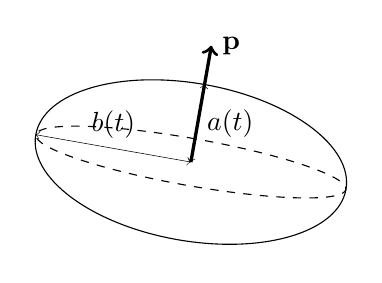
\begin{tikzpicture}[rotate=80]
        \draw(0,0) ellipse (1 cm and 2 cm);
        \draw[dashed](0,0) ellipse (0.3 cm and 2 cm);
        \draw[<->,very thin](0,0) --++ (1,0)node[midway,right]{$a(t)$};
        \draw[->,very thick](0,0) --++ (1.5,0)node[right]{$\textbf{p}$};
        \draw[<->,very thin](0,0) --++ (0,2)node[midway,above]{$b(t)$};
    \end{tikzpicture}
    \hfill
    \caption{Scheme of an  oblate spheroid oriented along the unit vector \textbf{p}.}
    \label{fig:scheme2}
\end{figure}
This tensor is defined such that its eigenvalues are the dimensionless square length of the semi-axis of the spheroid, such that $\textbf{C}_\alpha = a^2/r_0^2 \textbf{pp} + b^2 /r_0^2 (\textbf{I}-\textbf{pp})$ where $r$ is the radius of the sphere of same volume. 
This definition is convenient since it can be shown that $\textbf{C}_\alpha$ is equivalent to the Cauchy strain tensor well-defined in solid mechanics \citet{mwasame2017macroscopic}. 
Therefore, in a general coordinate system the point on the surface of the spheroid respect the equation, 
\begin{equation*}
    \textbf{r}\cdot\textbf{C}^{-1}\cdot\textbf{r} = r_0^2,
\end{equation*}
where $\textbf{C}$ is the inverse operator. 

Additionally, one can verify that the second order moment of mass of the particles is related to the conformation tensor through, $\textbf{M}_\alpha = \frac{m_\alpha  r_0^2}{5} \textbf{C}$. 
One can show that the constant volume constrain can be obtained by ensuring that $\text{det}(\textbf{C}) = (ab^2)^2 /(r_0^6) = 1$. 
It must be understood that at equilibrium the particle reach a spherical shape and therefore has $\textsc{C} = \textbf{I}$. 

\subsubsection*{The drop internal kinematic equation}



The evolution of $\textbf{C}_\alpha$ and $\bm\Gamma_\alpha$ will be described by the second moment of mass and first moment of momentum equation.
Consequently, we must reformulate the terms in \ref{eq:dt_M_alpha} and \ref{eq:dt_P_alpha} in terms of $\textbf{C}_\alpha$ and $\bm\Gamma_\alpha$. 
The integrals constitutive of these moments equations can be written, 
\begin{align}
    \intO{(\textbf{rw}_2^0 )_{ij}+ (\textbf{w}_2^0 \textbf{r})_{ij}} 
    = \textbf{C}_{\alpha,ik} \cdot \bm\Gamma_{\alpha,kj}
    +  \bm\Gamma_{\alpha,ki} \cdot \textbf{C}_{\alpha,jk}
    % +  \bm\Gamma_{\alpha,ij} + \bm\Gamma_{\alpha,ij}
    \\
    \intO{\rho_2 \textbf{w}_{2,i}^0\textbf{w}_{2,j}^0}
    = \frac{m_\alpha a^2}{5}
        \bm\Gamma_{\alpha,lj}\bm\Gamma_{\alpha,ki} \textbf{C}_{\alpha,kl} 
        % + \bm\Gamma_{\alpha,kj}\bm\Gamma_{\alpha,ki} 
        % + f_\textbf{ww}(\textbf{u}_\alpha,\textbf{C}_\alpha,\bm\Gamma_\alpha,\textbf{u}_1,\bm \Gamma_1,\phi_2)
        + \intO{\rho_2\textbf{w}^s_2\textbf{w}^s_2}
    \\
    \label{eq:sigma_2_def}
    \intO{\bm\sigma_{2,ij}^0}
    =
    % -\intO{p_2^0} \textbf{I}_{ij}
    \mu_2 v_\alpha (\bm\Gamma_{\alpha,ij} + \bm\Gamma_{\alpha,ij})
    + \mu_2 \intS{\textbf{w}^s_{2,i}\textbf{n}_{2,j}+ \textbf{w}^s_{2,j}\textbf{n}_{2,i}}
    + \textbf{I}_{ij}\intO{p_2^0} 
    \\
    \label{eq:sigma_I_def}
    \intS{\bm\sigma_{I,ij}^0}
    = \frac{2 \gamma v_\alpha }{a} \textbf{I}_{ij} - \frac{4 \gamma v_\alpha }{5 a} \textbf{C}_{\alpha,ij}
    +\mathcal(|\textbf{C}|^2)\\
    \intS{\textbf{r}\bm\sigma_1^0\cdot \textbf{n}_2}
    = 
    \frac{1}{2}\intS{(\textbf{r}\bm\sigma_1^0-\bm\sigma_1^0\textbf{r})\cdot \textbf{n}_2}
    + \frac{1}{2}\intS{(\textbf{r}\bm\sigma_1^0+\bm\sigma_1^0\textbf{r})\cdot \textbf{n}_2}
    % \textbf{M}(\textbf{u}_\alpha,\textbf{C}_\alpha,\bm\Gamma_\alpha,\textbf{u}_1,\bm \Gamma_1,\phi_2)
\end{align}
First, as discussed above only the deforming motion contribute to the symmetric part of the moment of momentum, we could therefore express it explicitly in terms of the particle unknown. 
Regarding the first moment of the surface tension, it has been computed analytically carrying a surface integral on the ellipsoidal surface of the droplet. 
Since, the droplets remain spheroidal under small deformation we choose to approximate $\intS{\bm\sigma_I^0}$ with its first order Taylor series in $\textbf{C}_\alpha$ without lost of generality.
Note that our expression of $\intS{\bm\sigma_I^0}$ is in agreement with \citet{lhuillier1987phenomenology} if one account for the slight difference of his definition of the deformation tensor which is half of $\textbf{C}_{\alpha}$. 
% in which our $\textbf{C}_\alpha$ is twice his, in the limit of small \textbf{C}_\alpha.
For the expression of $\intO{\rho_2 \textbf{w}_{2,i}^0\textbf{w}_{2,j}^0}$, $ \intO{\bm\sigma_{2,ij}^0}$ we had to introduce two unknown functions, $f_\textbf{ww}$, $f_{\bm{\sigma}}$, which vanish when $\textbf{w}^s_2 =0$. 
Therefore, these expressions are a sum of a function involving $\bm\Gamma_\alpha$ and an unknown part which depend on the parameters of the problem and need to be closed. 
The expression of $\intO{\rho_2 \textbf{w}_{2,i}^0\textbf{w}_{2,j}^0}$, $ \intO{\bm\sigma_{2,ij}^0}$ and $\intS{\textbf{r}\bm\sigma_1^0\cdot \textbf{n}_2}$ are very problem dependent. 
To provide a clearer example we computed these terms in \ref{ap:Translating_sphere} in the simplified scenario of an isolated droplet in a general linear flow. 
\begin{multline}    
    \frac{m_\alpha a^2}{10}\ddt^2 \textbf{C}_\alpha
    - \frac{m_\alpha a^2}{5}
    \bm\Gamma_{\alpha,lj}\bm\Gamma_{\alpha,ki} \textbf{C}_{\alpha,kl} 
    - \intO{\rho_2\textbf{w}^s_2\textbf{w}^s_2}\\
    + \mu_2 v_\alpha (\bm \Gamma_{p,ij}+\bm \Gamma_{p,ji})
    + \mu_2 \intS{\textbf{w}^s_{2,i}\textbf{n}_{2,j}+ \textbf{w}^s_{2,j}\textbf{n}_{2,i}}\\
    + \textbf{I}_{ij}\intO{p_2^0} 
    + \frac{2 \gamma v_\alpha }{a} \textbf{I}_{ij} 
    - \frac{4 \gamma v_\alpha }{5 a} (\textbf{C}_{ij} - \textbf{I}_{ij})
    =  
    + \frac{1}{2}\intS{(\textbf{r}\bm\sigma_2^0+ \bm\sigma_2^0\textbf{r})\cdot \textbf{n}}
\end{multline}
\begin{multline}    
    \frac{m_\alpha a^2}{10}\ddt^2 \textbf{C}_\alpha
    - \frac{m_\alpha a^2}{5}
    \bm\Gamma_{\alpha,lj}\bm\Gamma_{\alpha,ki} \textbf{C}_{\alpha,kl} 
    - \intO{\rho_2\textbf{w}^s_2\textbf{w}^s_2}\\
    + \mu_2 v_\alpha (
        \ddt \textbf{C}_{\alpha,ij}
         -(\textbf{C}_{\alpha,ik} - \textbf{I}_{ik}) \cdot \bm\Gamma_{\alpha,kj}
    -  \bm\Gamma_{\alpha,ki} \cdot (\textbf{C}_{\alpha,jk} - \textbf{I}_{\alpha,jk})
    )
    + \mu_2 \intS{\textbf{w}^s_{2,i}\textbf{n}_{2,j}+ \textbf{w}^s_{2,j}\textbf{n}_{2,i}}\\
    + \textbf{I}_{ij}\intO{p_2^0} 
    + \frac{2 \gamma v_\alpha }{a} \textbf{I}_{ij} 
    - \frac{4 \gamma v_\alpha }{5 a} (\textbf{C}_{ij} - \textbf{I}_{ij})
    =  
    + \frac{1}{2}\intS{(\textbf{r}\bm\sigma_2^0+ \bm\sigma_2^0\textbf{r})\cdot \textbf{n}}
\end{multline}
In the quasi steady regime all the derivative cancel out and $\bm\Gamma$ also,
\begin{multline}    
    % \frac{m_\alpha a^2}{10}\ddt^2 \textbf{C}_\alpha
    % - \frac{m_\alpha a^2}{5}
    % \bm\Gamma_{\alpha,lj}\bm\Gamma_{\alpha,ki} \textbf{C}_{\alpha,kl} 
    - \intO{\rho_2\textbf{w}^s_2\textbf{w}^s_2}
    + \mu_2 \intS{\textbf{w}^s_{2,i}\textbf{n}_{2,j}+ \textbf{w}^s_{2,j}\textbf{n}_{2,i}}\\
    + \textbf{I}_{ij}\intO{p_2^0} 
    + \frac{2 \gamma v_\alpha }{a} \textbf{I}_{ij} 
    - \frac{4 \gamma v_\alpha }{5 a} (\textbf{C}_{ij} - \textbf{I}_{ij})
    =  
    + \frac{1}{2}\intS{(\textbf{r}\bm\sigma_2^0+ \bm\sigma_2^0\textbf{r})\cdot \textbf{n}}
\end{multline}
Thus the stresslet might be computed upon known these integral but at this stage we could say ok just compute the stress let then. 
For bubbly flow we have the relation,
\begin{equation*}
+ \textbf{I}_{ij}\intO{p_2^0} 
+ \frac{2 \gamma v_\alpha }{a} \textbf{I}_{ij} 
- \frac{4 \gamma v_\alpha }{5 a} (\textbf{C}_{ij} - \textbf{I}_{ij})
=  
+ \frac{1}{2}\intS{(\textbf{r}\bm\sigma_2^0+ \bm\sigma_2^0\textbf{r})\cdot \textbf{n}}
\end{equation*}
In which case \textbf{C} is related to the pressure jump plus the stresslet while $\bm\Gamma$ isn't necessarily negligible. 

In this casethe stresslet appear to be, 
\begin{equation*}
    + \textbf{I}_{ij}\intO{p_2^0} 
    + \frac{2 \gamma v_\alpha }{a} \textbf{I}_{ij} 
    - \frac{4 \gamma v_\alpha }{5 a} (\textbf{C}_{ij} - \textbf{I}_{ij})
    - \mu_1 \intS{\textbf{w}^s_{2,i}\textbf{n}_{2,j}+ \textbf{w}^s_{2,j}\textbf{n}_{2,i}}
    - \mu_1 v_\alpha (\bm \Gamma_{p,ij}+\bm \Gamma_{p,ji})
    =  
    \intS{\textbf{r}\bm\sigma_2^0\cdot \textbf{n}}
    - \mu_1 \intO{e_2^0}
\end{equation*}
Then if we arrive to prove that $(\textbf{C}_{ij} - \textbf{I}_{ij}):\textbf{I}_{ij} = 0$ we recover a Laplace pressure like making $+ \textbf{I}_{ij}\intO{p_2^0} 
+ \frac{2 \gamma v_\alpha }{a} \textbf{I}_{ij} $ equal to the fluid pressure. 

At this point it wouldn't be wise trying to find an expression for each of these unknown functions in such a generality. 
Instead, we expose the unclosed set of equation of motions for spheroidal particles. 
In addition to the previously exposed equations (mass, momentum and energy equation) this system is constituted of three equations, one for $\textbf{C}_\alpha$ and two equation for the moment of momentum, the symmetric and skew-symmetric moment of momentum. 
% These read, 
% \begin{align*}
%     \ddt \textbf{C}_{\alpha,ij}
%     = \textbf{C}_{\alpha,ik} \cdot \bm\Gamma_{\alpha,kj}
%     +  \bm\Gamma_{\alpha,ki} \cdot \textbf{C}_{\alpha,jk},\\
%     \frac{a^2  m_\alpha}{5} \ddt( \textbf{C}_{ik} \cdot \bm\Gamma_{\alpha,kj}
%     -  \bm\Gamma_{\alpha,ki} \cdot \textbf{C}_{jk})
%     =  \intS{(\textbf{r}\bm\sigma_2^0- \bm\sigma_2^0\textbf{r})\cdot \textbf{n}}\\
%     \frac{m_\alpha a^2}{5}\ddt^2 \textbf{C}_\alpha
%     - \frac{m_\alpha a^2}{5}[
%     \bm\Gamma_{\alpha,lj}\bm\Gamma_{\alpha,ki} \textbf{C}_{\alpha,kl} + f_\textbf{ww}]
%     + \mu_2 v_\alpha [(\bm \Gamma_{p,ij}+\bm \Gamma_{p,ji})
%     + f_{\bm{\sigma}}]\\
%     + \frac{2 \gamma v_\alpha }{a} \textbf{I}_{ij} 
%     - \frac{4 \gamma v_\alpha }{5 a} (\textbf{C}_{ij} - \textbf{I}_{ij})
%     = \intS{(\textbf{r}\bm\sigma_2^0+ \bm\sigma_2^0\textbf{r})\cdot \textbf{n}}
%     % + \textbf{I}_{ij}\intO{p_2^0}
% \end{align*}
% Where we placed the unknown function at the right hands side of these equations. 
Now, we would like to propose a more intuitive interpretation of the mass and momentum equations.
To that end, we make the problem dimensionless by introducing, 
the \textit{Capillary number} $Ca= \frac{\mu_1 U}{\gamma}$, The viscosity ratio $\lambda = \mu_2/\mu_1$, the density ratio $\zeta = \rho_2/\rho_1$ and the Reynolds number $Re = \frac{a U \rho_1}{\mu_1}$, with $U$ as the velocity scale. 
%  such that  $\bm\Gamma_\alpha'  = \frac{a}{U}\bm\Gamma$, and $\tau_a$ the timescale related to the drop shape evolution.
In the low Reynolds regime the first moment of surface traction forces will be proportional to a viscous stress (see \ref{ap:Translating_sphere}), therefore :$\intS{\textbf{r}\bm\sigma_2^0\cdot \textbf{n}} =\mu_1  \tau v_\alpha \intS{\textbf{r}\bm\sigma_2^0\cdot \textbf{n}}^*$, with $\tau$ the inverse timescale of the external solicitation.
The ratio between the external flow scale $\tau$ and the drop timescale $\tau_a$ is noted $\beta$. 
With that in mind, \ref{eq:dt_M_alpha}, \ref{eq:dt_mu_alpha} and \ref{eq:dt_S_alpha} might be written :
\begin{align}
    \label{eq:dt_Cs}
    \beta \ddt \textbf{C}_{\alpha,ij}
    - \textbf{C}_{\alpha,ik} \cdot \bm\Gamma_{\alpha,kj}^*
    - \bm\Gamma_{\alpha,ki}^* \cdot \textbf{C}_{\alpha,jk},
    = 
    \bm\Gamma_{\alpha,ij}^*
    +  \bm\Gamma_{\alpha,ji}^*\\
    Re \zeta \beta \ddt( \textbf{C}_{\alpha,ik} \cdot \bm\Gamma_{\alpha,kj}^*
    -  \bm\Gamma_{\alpha,ki}^* \cdot \textbf{C}_{\alpha,jk}
    + \bm\Gamma_{\alpha,ji} - \bm\Gamma_{\alpha,ij})
    =  \intS{(\textbf{r}\bm\sigma_2^0- \bm\sigma_2^0\textbf{r})\cdot \textbf{n}}^*\\
    \zeta Re \frac{1}{5}  
    \left[
        \frac{1}{2}\beta^2 \ddt^2_* \textbf{C}_\alpha
        - \bm\Gamma_{\alpha,lj}^* \bm\Gamma_{\alpha,ki}^* \textbf{C}_{\alpha,kl}^* 
        - \bm\Gamma_{\alpha,kj}^* \bm\Gamma_{\alpha,ki}^* 
        - f_\textbf{ww}
    \right]\nonumber\\
    + \lambda \left[
        \beta \ddt \textbf{C}_{\alpha,ij}
        -\textbf{C}_{\alpha,ik} \cdot \bm\Gamma_{\alpha,kj}
        - \bm\Gamma_{\alpha,ki}^* \cdot \textbf{C}_{\alpha,jk},
        + f_{\bm{\sigma}}
    \right]\nonumber\\
    - \frac{1}{Ca}\left[
        \frac{4}{5} \textbf{C}_{\alpha,ij}
        +2 \textbf{I}_{ij} 
    \right]
    =
    \frac{1}{2}\intS{(\textbf{r}\bm\sigma_1^0+ \bm\sigma_1^0\textbf{r})\cdot \textbf{n}}^*
    \label{eq:dt2_C}
\end{align}







The drop internal velocity will be assumed to be linear and homogeneous such as if it was a solid deformable displacement. 
It must be said that due to the presence of surface tension and relative velocity this hypothesis isn't physical. 
Indeed, on one hand inhomogeneous stresses such as surface tension stress, might induce inhomogeneous internal flow \citep{goddard1967nonlinear}, and obviously the relative motion will evidently induce a Hill's vortex-like internal motions. 
Therefore, in a second step the modeling of internal flow will include quadratic terms but for ow we restrict our attention to linear internal flow fields. 
Taking into account this assumption the drop internal velocity field can be written,
\begin{equation}
    \textbf{w}_2^0(\textbf{x}_\alpha)
    = \bm\Gamma_\alpha \cdot \textbf{r}
    =\bm{\Omega}_\alpha\cdot \textbf{r}
    + \textbf{E}_\alpha \cdot \textbf{r}
    \label{eq:def_vel}
\end{equation}
where $\bm\Gamma_\alpha$, is the velocity gradient for any point inside the domain $\Omega_\alpha(t)$, and $\textbf{E}_\alpha$ represents the rate of strain or the symmetric part second order tensor, and $\bm\Omega_\alpha$ the angular velocity pseudo vector. 

The evolution of the internal kinematic of the droplet, i.e. the shape, will be described by the second moment of mass equation, to which we substitute the tensor $\mathcal{M}_\alpha$ by \textbf{C} to obtain an equation for the deformation. 
It yields, 
\begin{equation*}
    \ddt \textbf{C}_{ij}
    = \textbf{C}_{ik} \cdot \bm\Gamma_{\alpha,kj}
    +  \bm\Gamma_{\alpha,ki} \cdot \textbf{C}_{jk}.
    \label{eq:dt_C}
\end{equation*}
From this point one can relate $\bm\Gamma_{\alpha,kj}$ to the fluid mean kinematic properties. 
In pure shear flow for example, if one consider the problem of a slightly deformable droplet one can show that, $\bm\Gamma \sim \Gamma_1(\textbf{x}_\alpha)$ where $\bm\Gamma_1$ is the local fluid velocity gradient.
From this consideration one can find back the classical models such as the one of  \citet{maffettone1998equation,schowalter1968rheological}. 

In our current problem, rising inertial droplets, we must thus seek for an expression linking the drop internal velocity gradient $\bm\Gamma_\alpha$ with the relative motion $\textbf{u}_{pf}$. 
This is done through the consideration of the second moment of momentum equation. 

\subsubsection*{The dynamical droplet equations}

Objective : 
\begin{equation*}
    \bm\sigma 
    = 
    - \phi_1 p_1 \textbf{I}
    - \mu_1 \textbf{e}
    + \phi_2(\bm\sigma_2 - \bm\sigma_1)
    + \phi_I\bm\sigma_I
\end{equation*}

The dynamic of the droplet will be described by the use of the symmetric moment of momentum equation presented in \ref{sec:Lagrangian}.
We will therefore need constitutive equation for the particle internal and surface stress. 
The particle internal stress is described by a Newtonian behavior law yielding directly, 
\tb{hypothèse}
\begin{equation*}
    \intO{\bm\sigma_2^0}
    = - \intO{p_2^0} \delta_{ij}
    + v_\alpha \mu_2 \textbf{E}_{\alpha,ij}.
\end{equation*} 
Equally, if the particle were constituted of any other material one could include the adapted constitutive law in this term. 
Regarding the particle surface stress, it can be computed analytically since we assumed a spheroidal shape. 
% Indeed, all the points on the surface of the particle can describe by the equation, $\textbf{r}\cdot\textbf{C}^{-1}-1=0$ which mean that the normal vector at the surface can be express as $\textbf{n}_2 = 2\textbf{H}\cdot\textbf{r}$ and it follow the tensorial expression of the local stress. 
The details are not given here but the results at $\mathcal{O}(|\textbf{C}|^3)$  and $\mathcal{O}(|\textbf{C}|^2)$ accurate yield, 
\begin{align*}
    \pSavg{\bm\sigma_I^0}
    &= \frac{\gamma v 2}{r} \left[
        1  + \frac{1}{20 } (\textbf{C}_{-\textbf{I}}:\textbf{pp})^2 
        + \frac{4}{20 } [\textbf{C}_{-\textbf{I}}:(\textbf{I}-\textbf{pp})]^2\right] \textbf{I}\\
        &- \frac{\gamma v}{35 r} \left[ 28 \textbf{C}_{-\textbf{I}}
        + 4[\textbf{C}_{-\textbf{I}}\cdot \textbf{C}_{-\textbf{I}} + 15 (\textbf{C}_{-\textbf{I}}:\textbf{pp})^2\textbf{pp}]
        \right]
        +\mathcal{O}(|\textbf{C}|^3)\\
    &= \frac{\gamma v 2}{r} \textbf{I} - \frac{\gamma v 4}{5 r} (\textbf{C} - \textbf{I})
    +\mathcal(|\textbf{C}|^2)
\end{align*}
Notice that the first term of the first equality correspond to $\frac{2\gamma}{3}s_\alpha$, it is therefore $\frac{2}{3}$ of the surface energy which varies only at $\mathcal{O}(|\textbf{C}|^2)$. 
The second term account for the deviatoric part of the stress tensor which is of $\mathcal{O}(\textbf{C})$. 
The results at first order are agreements with \citet{lhuillier1987phenomenology} when accounting for the different definition of the conformation tensor \textbf{C} that he used.

The moment of momentum equation with an internal velocity such as it is described by \ref{eq:def_vel} is then given by the expression,
\begin{multline}
    \ddt (\textbf{C}_{\alpha,ik} \bm\Gamma_{\alpha,kj})
    -\bm\Gamma_{\alpha,lj}\bm\Gamma_{\alpha,ki} \textbf{C}_{\alpha,kl}
    = 
    % \intO{p_2^0} \delta_{ij}
    - \frac{5\mu_2}{a^2\rho_2}  \textbf{E}_{\alpha,ij}
    + \frac{\gamma 6 }{\rho_2 a^3} \textbf{I} 
    - \frac{\gamma 4}{\rho_2 a^3} \textbf{C}_{\alpha,ij} 
    +\frac{5}{a^2 \rho_2 v_\alpha} \pavg{\textbf{r}\bm\sigma_1^0\cdot\textbf{n}_2}_{ij},
    \label{eq:moment_of_momentum}
\end{multline}
Or its symmetric part,
\begin{multline}
    \ddt^2 (\textbf{C}_{\alpha,ik})
    - 2\bm\Gamma_{\alpha,lj}\bm\Gamma_{\alpha,ki} \textbf{C}_{\alpha,kl}
    = 
    % \intO{p_2^0} \delta_{ij}
    - 2\frac{5\mu_2}{a^2\rho_2}  \textbf{E}_{\alpha,ij}
    + 2\frac{\gamma 6 }{\rho_2 a^3} \textbf{I} 
    - 2\frac{\gamma 4}{\rho_2 a^3} \textbf{C}_{\alpha,ij} 
    + 2\frac{5}{a^2 \rho_2 v_\alpha} \pavg{\textbf{r}\bm\sigma_1^0\cdot\textbf{n}_2}_{ij},
    \label{eq:moment_of_momentum}
\end{multline}
\tb{The internal velocity is way more to complicated one must use Hill vortex}
\tb{The isotropic part might cancel the difference in pressure.}
where the only undetermined term is the first moment of the hydrodynamic forces. 
While deriving \ref{eq:moment_of_momentum} we made absolutely no hypothesis on the dilute nature of the flow nor on its potentially inertial effect.
Therefore, solely the first moment of hydrodynamic force might be able to take in account the effect of finite volume fraction, inertial effect, particle interaction\ldots
Therefore we introduce the function,
\begin{align*}
    \pavg{\textbf{r}\bm\sigma_1^0\cdot\textbf{n}_2}_{ij}
    = \textbf{f}_{1,ij}(\textbf{u}_\alpha - \textbf{u}_1,\bm\Gamma_\alpha - \bm\Gamma_1, \textbf{C}_{\alpha},Re,\phi) 
\end{align*}
which depends on the particles fluid relative properties, $(\textbf{u}_\alpha - \textbf{u}_1,\bm\Gamma_\alpha - \bm\Gamma_1)$ and problem dimensionless number $Re,\phi$. 
Such a relation have been found in \citet{goddard1967nonlinear}. 

In \citet{raja2010inertial} they consider a deformable drop in shearing inertial flow. 
Their expression (3.18) for the particle contribution to the suspension stress is in fact a combination of \ref{eq:moment_of_momentum} and \ref{eq:dt_C} where the first moment $\pavg{\textbf{r}\bm\sigma_1^0\cdot\textbf{n}_2}_{ij}$ have been solved analytically in terms of $\bm\Gamma_1$.

Therefore, in the continuity of their work we now wish to determine $\pavg{\textbf{r}\bm\sigma_1^0\cdot\textbf{n}_2}_{ij}$ in a pure translating motion with no mean shear. 
It is known from the singularity solution of stokes flow that $\pavg{\textbf{r}\bm\sigma_1^0\cdot\textbf{n}_2}_{ij} = 0$ for a non-inertial spherical droplet in pure translation. 
However, when finite inertia effects appear the first moments of surface traction is not null and the drop deform into a spheroid proportionally the relative velocity $\textbf{u}_{fp}$. 


\subsubsection*{Determination of the shape based on \citet{taylor1964deformation} theoretical results}

In the last section we assumed an arbitrary spheroidal drop within a suspension. 
Now we consider that the drop is only subject to a relative motion with the fluid. 
Our goal is still to express the stress within the suspension. 

In \citet{taylor1964deformation} they derive the shape and the drag force of a translating droplet at $\textbf{O}(Re^2)$ in a steady state situation. 
Although they did not directly derive the stress let they provide a formula for the shape as a function of the relative velocity. 
In \citet{taylor1964deformation} they give an explicit formula for the deformation in terms of the Reynolds number $Re$ based on the relative velocity fields, $\textbf{u}_\alpha - \textbf{u}_1$. 
The dimensionless radius of the droplets can be express in the polar coordinate reference frame of the drop as, 
\begin{equation*}
    \frac{R_\text{taylor}(\theta)}{a} = 1 - \beta \textit{We} P_2(\cos\theta)
    + \mathcal{O}(Re^3)
\end{equation*}
where $Re = |\textbf{u}_{pf}| a /\nu_1$, $P_2(\cos\theta)$ is the Legendre polynomial of degree two and $\kappa$ is a coefficient related to physical parameters given in \citet{taylor1964deformation}.  
This solution need to satisfy $\kappa Re \ll 1$ and $Re \ll 1$ to be valid. 
These, 
% \begin{center}
%     \begin{tikzpicture}[gradient arrow/.style={
%         insert path={coordinate[pos=#1,sloped,
%             above=\pgfkeysvalueof{/tikz/ga/above}]  (aux-1)
%            coordinate[pos=#1,sloped,
%             above=\pgfkeysvalueof{/tikz/ga/above}+\pgfkeysvalueof{/tikz/ga/length}] (aux-2)
%            (aux-1) edge[/tikz/ga/arrow] 
%            (aux-2)}},ga/.cd,
%            above/.initial=3pt,
%            length/.initial=12pt,
%            arrow/.style={-stealth,black,solid,thick}]
%          \begin{axis}[scale=0.85,xmin=-4,xmax=12, ymin=-4,ymax=4,x=1cm,y=1cm,at={(-4cm,-4cm)}]
%           \addplot +[no markers,name=contour,
%            raw gnuplot,
%            thick,dashed,
%            empty line = jump, % not strictly necessary, as this is the default behaviour in the development version of PGFPlots
%            ] gnuplot {
%                set contour base;
%                set cntrparam levels discrete -2,-1.1,-1.4;
%                unset surface;
%                set view map;
%                set isosamples 500;
%                set samples 500;
%                splot -2/sqrt((x-7.5)^2+y^2)-3/sqrt((x-0.5)^2+y^2);
%            } 
%         %    [pos segment=1]
%         %    [gradient arrow/.list={0.2,0.8}]
%         %    [pos segment=3,/tikz/ga/arrow/.append style={red},/tikz/ga/length=10pt]
%         %    [gradient arrow/.list={0.2,0.8}];
%          \end{axis}
%     \end{tikzpicture}
% \end{center}
Upon assuming a quasi steady state regime which correspond to a droplet response time $\frac{1}{\tau_a^2} \ll \frac{\mu_1 U \lambda }{a^3\rho_2} \approx \frac{\mu_1 U \lambda }{a^3\rho_2 Ca} \approx \frac{\mu_1 U \lambda }{a^3\rho_2}$ we can stipulate that the shape of the droplet is instantaneously correlated with the velocity. 
In this hypothesis it is clear that the shape of the droplet is correlated at any time with the local motion of the flow $\textbf{u}_{fp}$. 
The conformation tensor principal values, are related to \citet{taylor1964deformation} formula through,
\begin{align*}
    \textbf{C}(\textit{We})
    % = \left(\frac{R_\text{taylor}(0)}{a}\right)^2
    = (1 - \beta \textit{We} )^2 \textbf{pp}
    + 
     (1 + \beta \textit{We}/2  )^2 (\textbf{I}-\textbf{pp})
\end{align*}
where $\textit{We}$ is the \textit{Weber} number defined as $\textit{We} = \rho_1 a \textbf{u}_{\alpha f}\cdot\textbf{u}_{\alpha f}/\sigma$. 

Now that we obtained the shape as a function of the relative velocity, we aim to recover the rate of deformation of the drop through the second moment of mass equation. 
The droplet interior flow is a complex function of space and time. 
We assumed small deformation such that our spherical particle become a spheroid. 
Therefore, the velocity fields responsible for the shape change is a linear function of the position, thus $\textbf{w}_2^0 = f(\textbf{r}) + \bm\Gamma_\alpha(t,\FF) \cdot \textbf{r}$, where $f(\textbf{r})$ is the steady state internal motion and $\bm\Gamma_\alpha(t,\FF)$ is a time dependent matrix describing the homogeneous deformation of the droplets. 
The complex recirculation structure such as Hill vortexes-like doesn't contribute to the symmetric part of the moment of momentum as it is not changing the shape of the particle. 
The only contribution to the stretching of momentum is therefor the second term. 
Additionally, we always consider the drop deformation in the direction of the flow. 
Now that the drop shape is fully determined by the local Reynolds number the second order of mass equation can be use to determine the inner rate of strain of the drop,
\begin{equation*}
    \ddt \textbf{C}_{ij}
    = \textbf{C}_{ik} \cdot \bm\Gamma_{\alpha,kj}
    +  \bm\Gamma_{\alpha,ki} \cdot \textbf{C}_{jk}.
\end{equation*}
This equation must be solved for the $\Gamma_{ki}$ as $\textbf{C}$ is a known function of $\textbf{u}_{pf}$ and the physical parameters. 

As mentioned above the surface tension stress can be estimated to be an instantaneous function of \textbf{C}, namely, 
\begin{align*}
    \pSavg{\bm\sigma_I^0}
    = \frac{\gamma v 2}{r} \textbf{I} - \frac{\gamma v 4}{5 r} (\textbf{C} - \textbf{I})
    +\mathcal(|\textbf{C}|^2)
\end{align*}
At this stage the only remaining term to determine the contribution to the suspension stress is an expression of the particle stress tensor as a function of \textbf{C} ad $\bm\Gamma$. 
The symmetric part of the moment of momentum equation can be written,
\begin{equation*}
    \ddt^2\intO{\textbf{C}_{ij}}
    -\intO{\rho_2\textbf{w}_{2,i}^0\textbf{w}_{2,j}^0}
    + \intO{\bm\sigma_{2,ij}^0}
    + \intS{\bm\sigma_{I,ij}^0}
    = \intS{(\textbf{r}\bm\sigma_1^0+ \bm\sigma_1^0 \textbf{r})_{ijk}\cdot \textbf{n}_{2,k}}
\end{equation*}
At this stage we must either find the complete closure for $\textbf{w}_{2,i}^0$ which will enable us to find an expression for one of the two remaining terms.
And by solving this equation one might obtain the last one terms in terms of $\bm\Gamma$ and \textbf{C}. 
\tb{Either find the singularity sol or assume linear displacement}

We're assuming that the rate of strain is the only contribution to the stress, which might be justified by the fact that Hill's vortexes resultant vanish for spherical drops. 
Thus, the drop interior stress might be written, 
\begin{equation*}
    \pSavg{\bm\sigma_2^0}
    =-\pOavg{p_2^0} 
    + \mu_2 n_p (\bm\Gamma_{p,ij}+\bm\Gamma_{p,ji})
\end{equation*}
Then the set of equation needed to describe the rheology of a dilute suspension of inertial drops is, 
\begin{align*}
    \textbf{C}_p(\textit{We})
    % = \left(\frac{R_\text{taylor}(0)}{a}\right)^2
    = (1 - \beta \textit{We} )^2 \textbf{pp}
    + 
     (1 + \beta \textit{We}/2  )^2 (\textbf{I}-\textbf{pp})\\
    \pavg{\ddt \textbf{C}_{ij}}
    = \textbf{C}_{p,ik} \cdot \bm\Gamma_{p,kj}
    +  \bm\Gamma_{p,ki} \cdot \textbf{C}_{p,jk}.\\
    \bm\sigma^\text{dev}
    = 
    \mu_1 \textbf{e}_{ij}
    +  n_p (\mu_2 - \mu_1) (\bm\Gamma_{p,ij} + \bm\Gamma_{p,ji})
    + n_p \frac{\gamma  4}{5 r} (\textbf{C}_{p,ij} - \textbf{I}_{ij})
\end{align*}

Under this assumption it is observed that $\textbf{C}\sim U^2$ has the same form as the pseudo turbulence Reynolds stress computed in potential flow. 
Indeed, 
The deviatoric part of the conformation tensor can be written exactly as, 
\begin{equation*}
    \textbf{C} - \textbf{I}  = - 3 \beta \textit{We} \textbf{pp} +  \beta \textit{We} \textbf{I}
    + (\beta^2 \textit{We}^2 3/4) \textbf{pp} + \beta^2 \textit{We}^2/4 \textbf{I} 
\end{equation*}
We now stipulate that the deformation occur in the direction of the velocity difference such that the relative phase velocity of the particle $\alpha$ is written, $\textbf{u}_{\alpha f} = |\textbf{u}_{\alpha f}|\textbf{p}$, in this case the conformation tensor can be expressed, 
\begin{equation}
    \textbf{C}(\textbf{u}_{\alpha f}) - \textbf{I}  =  \frac{ \rho_1 a \beta}{\gamma} \left[
        -  3
        \textbf{u}_{\alpha f}\textbf{u}_{\alpha f}+   \textbf{u}_{\alpha f}\cdot\textbf{u}_{\alpha f}\textbf{I}
    \right]
    +\textbf{u}_{\alpha f}\cdot\textbf{u}_{\alpha f}\left(\frac{ \beta \rho_1 a}{\gamma}\right)^2
    \left[
        \frac{3}{4}
        \textbf{u}_{\alpha f}\textbf{u}_{\alpha f}
        +
        \frac{1}{4}
        \textbf{u}_{\alpha f}\cdot\textbf{u}_{\alpha f}
        \textbf{I}
    \right]
    \label{eq:C_def_with_u}
\end{equation}
This tensor is the particle confirmation tensor of the particle $\alpha$. 
We now apply an average procedure, and by that, $\pavg{\textbf{u}_{\alpha f}\textbf{u}_{\alpha f}} = \textbf{u}_{pf}\textbf{u}_{pf} + \pavg{\textbf{u}_\alpha'\textbf{u}_\alpha'}$ to gather with the assumption that the higher order fluctuation terms becomes negligible we obtain, 
\begin{multline*}
    \textbf{C}_p - \textbf{I}  =  \frac{ \rho_1 a \beta}{\gamma} \left[
        -  3
        \textbf{u}_{\alpha f}\textbf{u}_{\alpha f}
        +   (\textbf{u}_{\alpha f}\cdot\textbf{u}_{\alpha f})\textbf{I}
    \right]\\
    +\textbf{u}_{\alpha f}\cdot\textbf{u}_{\alpha f}\left(\frac{ \beta \rho_1 a}{\gamma}\right)^2
    \left[
        \frac{3}{4}
        \textbf{u}_{p f}\textbf{u}_{p f}
        +
        \frac{1}{4}
        (\textbf{u}_{p f}\cdot\textbf{u}_{p f})
        \textbf{I}
    \right]
    + \pavg{\textbf{C}(\textbf{u}_\alpha')}
\end{multline*}
where the last term correspond to \ref{eq:C_def_with_u} with $\textbf{u}_\alpha'$ is input velocity. 
Under these quite restrictive assumption we have shown that the surface tension contribution to the bulk stress have the same functional form as the Reynolds stress in potential flows \citet{van1982bubble}. 
% \section*{fluid phase stress}
Already, we can see that the equivalent stress of the fluid phase is the made of the average fluid stress represented by the two first terms on the right hands side of \ref{eq:sigma_eq_0}. 
The first moment $\pSavg{\textbf{r}\bm{\sigma}_1^0 \cdot \textbf{n}_2}$ appearing in \ref{eq:sigma_eq_0} posses a skew-symmetric part and a symmetric part, the latter corresponding to the stresslet (see \ref{eq:stresslet_def}).
However, for non-solid particles \ref{eq:stresslet_def} is not entirely valid since in stokes theory the quantity referred as the stresslet is defined as \citet{pozrikidis1992boundary,kim2013microhydrodynamics},
\begin{equation}
    \label{eq:stresslet_def}
    n_p \mathscr{S}_{p,ki}
    = \frac{1}{2}
    \pSavg{
        r_k \sigma_{il}n_l + r_i \sigma_{kl}n_l 
        - \delta_{ik}
        \frac{2}{3}
        r_l \sigma_{lk}n_k
        - 2 \mu_f (u_k n_i+u_i n_i)
    }
\end{equation}
Likewise, we introduce the average skew symmetric part $\mathscr{L}_p$ and the average trace of the first moments $\mathscr{D}_p$ such as, 
\begin{align}
    \label{eq:torque_def}
    n_p \mathscr{L}_{p,ki}
    = \frac{1}{2}\pSavg{ r_k \sigma_{il}n_l - r_i \sigma_{kl}n_l }\\
    \label{eq:trace_def}
    n_p \mathscr{D}_{p,ij}
    = \frac{1}{3}\pSavg{ r_k (\sigma_{kl} + p_1 \delta_{kl})n_l } \delta_{ij}
    - n_p v_p p_1 \delta_{ij}
\end{align}
where we have retrieved the mean pressure from the trace of the first moments, so that we make appear the hydrostatic pressure  $n_p v_p p_1 \bm\delta$ explicitely.  
Notice that the volume fraction $\phi_1$ is present in front of the averaged pressure terms in \ref{eq:sigma_eq_0}.  
In various study \citep{prosperetti2009computational,chu2016flux}, this term is shown to be problematic  since it might generate nonphysical flux of momentum. 
However, as shown above and pointed out by  \citet{zhang1997momentum,jackson1997locally}, the first moment of hydrodynamic force tensor contains a part of the hydrostatic pressure.
With that contribution the total pressure in the fluid stress reach $\phi_1p_1 + n_p p_1 \approx p_1$ which is consistent.
Additionally, as seen in \ref{sec:two-fluid} the Reynolds stress is related to the pseudo turbulent kinetic energy through $\avg{\chi_1 \rho_1\textbf{u}_1'\textbf{u}_1'} : \bm\delta = 2k_1$ . 
Therefore, we can write, $\avg{\chi_1 \rho_1\textbf{u}_1'\textbf{u}_1'} = 2 \rho_1 k_1 \bm\delta + \avg{\textbf{u}_1'\textbf{u}_1'}^\text{dev}$ where the second term is the deviatoric part of the Reynolds stress. 

These remarks motivate us to rewrite the equivalent fluid phase stress under the general expression,  
\begin{multline*}
    \bm{\sigma}_1^\text{eq}
    = 
    \underbrace{p_1  \bm\delta
    - \mu_1 \textbf{e} }_\text{Newtonian fluid stress}
    +  \underbrace{\phi_1 k_1 \bm\delta
    + \rho_1 \avg{\chi_1\textbf{u}_1'\textbf{u}_1'}^\text{dev}}_\text{fluctuating stresses}
    - \underbrace{(n_p \mathscr{S}_p
    + n_p \mathscr{L}_p
    + n_p \mathscr{D}_p )}_\text{interfacial particles stresses}\\
    % + \mu_1  \pSavg{{\textbf{u}_1\textbf{n}_2 + \textbf{n}_2 \textbf{u}_1}}
    % - n_p \textbf{F}_\text{p}
    % + n_p \textbf{F}_\text{pfp} 
    + \frac{1}{2} \div \underbrace{\left[
        \pSavg{\textbf{rr}\bm{\sigma}_1^0\cdot \textbf{n}_2}
        + 2\pOavg{\mu_1 \textbf{re}_2^0 }
        + \ldots
        \right]
        }_\text{inhomogeneous particles stresses}
    \label{eq:sigma_eq1_def}
\end{multline*}
% with, 
% \begin{equation*}
%      \bm{\Sigma}
%     = 
%      \pMSavg{\textbf{rr} \bm{\sigma}_1^0\cdot \textbf{n}_2}
%      -\pMOavg{\mu_1 \textbf{r} \textbf{e}_2 }\\
% \end{equation*}
The contribution of the fluid phase equivalent pressure is made of,
the averaged $p_1$, the fluctuating part of the moment of force traction $\mathscr{D}_p$, and the fluid pseudo turbulent energy, $\phi_1 k_1$. 
The deviatoric part of the stress is constituted of the deviatoric part of the Reynolds stress $\avg{\chi_1\textbf{u}_1'\textbf{u}_1'}^\text{dev}$, the mean fluid shear rate $\mu_1 \textbf{e}$, the stresslet $\mathscr{S}_p$ and the hydrodynamic torque $\mathscr{L}_p$. 
The higher order moments found in $\bm{\Sigma}$ are not necessarily negligible, as shown in \citet{lhuillier1996contribution,jackson1997locally}, in fact they exhibit a different physical meaning. 
The first order moments will be function of the mean gradient of the fluid velocity while the other will be function of the background relative motion. 

\tb{a enlever}
It is known that the $n_p \mathscr{S}_p$ plays a significant role in the determination of the equivalent viscosity of the mixture. 
Therefore, it is of major importance to be able to measure it in DNS or experiment.
As, demonstrated by the expression of the ensemble averaged stress it is quite difficult to obtain such an information by experimental means, since it is mixed among other stresses.  
In DNS however we have access to pretty much any information, nevertheless surface integration of the stress can be shown to be inaccurate when performing volume of fluid method. 
Therefore, we propose the following formulas based on \ref{eq:dt_hybrid_Sp} which enable us to compute the stresslet by almost only volume integration,  


The last integral accounting for surface tension cannot be converted to volume integral. 
However, this integral is related only to the geometry of the interface. 
Besides, note that the pressure is absent as $\mathscr{S}_p$ is traceless. 

\begin{multline}    
    + n_p \mathscr{S}_p
    =
    \frac{1}{2}\pavg{\ddt^2{\textbf{M}_\alpha^\text{dev}}}
    - \pOavg{\left(
    \rho_2\textbf{w}_2^0 \textbf{w}_2^0
    - \rho_2\frac{1}{3}(\textbf{w}_2^0 \cdot \textbf{w}_2^0)\bm\delta\right)}\\
    + \mu_1 (\lambda - 1)\pOavg{\textbf{e}_2^0}
    + \pSavg{\gamma\left(\frac{1}{3}\bm\delta-\textbf{nn}\right)}\\
\end{multline}



\subsection{The bulk stress in dispersed multiphase flow}



Now that the architecture of the averaged dispersed multiphase flow equation is clarified, we would like to present the expression of the bulk stress tensor in a suspension of inertial particles subject to an arbitrary local body force field, $\textbf{b}^0$.
Firstly, is important to recall the definition of the \textit{bulk stress}. 
We define the \textit{bulk stress} tensor as a force applied on the fluid and on the particles phase, having the form $\div \bm{\Sigma}$, which added to the total external force $\textbf{B}$, balance exactly the material derivative of the mixture momentum : $\frac{D \rho \textbf{u}}{Dt}$. 
In this definition $\textbf{B}$ cannot be decomposed into a vector and a divergence of a tensor, in which case the latter would just contribute to $\bm{\Sigma}$.

We first expose the averaged mixture momentum and angular momentum equation easily derived from \ref{eq:dt_avg_f}, 
\begin{align}
    \pddt (\rho u_i)
    + \partial (\rho u_iu_k
    + \sigma_{ik}^\text{eq})
    = b_i\\
    \epsilon_{ijk} \sigma_{jk}
    = 0 
    \label{eq:momentum_bulk}
\end{align}
In the momentum equation we have defined, $\sigma_{ik}^\text{eq} = \avg{\rho\textbf{u}'\textbf{u}'}
- \avg{\chi_1\bm{\sigma}_1^0}-\avg{\chi_2\bm{\sigma}_2^0} - \avg{\delta_I \bm{\sigma}_I^0}$. 
Additionally, in the averaged angular momentum equation we have assumed that no-body torque exist at the local scale making the second equality equal to $0$ \citet{leal2007advanced} and the averaged mixture stress $\bm{\sigma}$ a symmetric quantity. 
However, note that $\bm{\sigma}$ is not exactly equal to the \textit{bulk stress} tensor $\bm{\Sigma}$ since $\textbf{b}$ can be expressed as a divergence of a stress.
Indeed, have defined $\textbf{b} = \textbf{B} + \div  \pMOavg{\textbf{b}_2^0}$ where $\textbf{B} = \phi_1 \textbf{b}_1 +  \pOavg{\textbf{b}_2^0 }$ and  $\pMOavg{\textbf{r}\textbf{b}_2^0}$ is defined accordingly to the previous definition. 
It follows the definition of the \textit{bulk stress} : 
\begin{equation}
    \bm{\Sigma}
    = 
    \avg{\rho\textbf{u}'\textbf{u}'}
    - \avg{\chi_1\bm{\sigma}_1^0}
    - \avg{\chi_2\bm{\sigma}_2^0} 
    - \avg{\delta_I \bm{\sigma}_I^0}
    - \pMOavg{\textbf{r}\textbf{b}_2^0}
\end{equation}
which proves already, in the absence of particles moments of the body forces $\pMOavg{\textbf{r}\textbf{b}_2^0}$, the antisymmetric part of the suspension stress is null, in agreement with \citet{dolata2020heterogeneous}.
% This skew symmetric part can be written in vector form as, 
% \begin{equation*}
%     \epsilon_{ijk}\textbf{T}_{jk}
%     = 
%     -\epsilon_{ijk} \pOavg{r_kb_j}
%     -\epsilon_{ijk}\frac{1}{2}\partial_l \pOavg{r_lr_kb_j}
%     = 0  
% \end{equation*}
We recall that the carrier fluid is a Newtonian fluid, therefore we may express the fluid phase stress as, 
\begin{equation}
    \phi_1 \sigma_{1,jk}
    = -p_1 \delta_{jk}
    + \mu_1 e_{jk}
    - \mu_1 \phi_2 e_{2,jk}. 
\end{equation} 
Additionally, we use the methodology of \citep{lhuillier1992volume,lhuillier1996contribution} to re express the averaged particle stress terms. 
The divergence of the particle phase stress may be expressed using \ref{eq:f_exp}, 
\begin{align}
    \label{eq:exp_sigma22}
    \partial_k \avg{\chi_2 {\sigma}_2^0}_{ik}
    &=  \partial_k\pOavg{ {\sigma}_{2,ik}^0}
    -\frac{1}{2} \partial_k\partial_j
    \pOavg{ r_j{\sigma}^0_{2,ik} + r_k\sigma^0_{2,ij}}
    + \ldots  \\
    \label{eq:exp_sigmaI2}
    \partial_k \avg{\delta_I {\sigma}^0_I}_{ik} 
    &=  \partial_k\pSavg{ {\sigma}_{I,ik}^0 }
        -\frac{1}{2} \partial_k\partial_j \pSavg{ r_j {\sigma}_{I,ik}^0+r_k {\sigma}_{I,ij}^0 }
        + \ldots  
\end{align}
Note that the heterogeneous terms must remain symmetric in the index $kj$ due to the double contraction with the operator $\partial_k\partial_j$, thus only the symmetric part in $jk$ remain and the terms such as, $\pOavg{ r_j{\sigma}^0_{2,ik} - r_k\sigma^0_{2,ij}}$ vanish. 
Upon the use of the moment of momentum equation of the first and second order we can easily derive these expressions, 
\begin{align}
    \intS{ (\bm{\sigma}_I)_{ik}}
    +\intO{ (\bm{\sigma}_2^0)_{ik}}
    = 
    \intO{ \rho_2 
    (\textbf{w}_2^0\textbf{w}_2^0  )_{ik}
    }
    -\ddt \intO{ r_i (\textbf{u}^0_2)_k }
    +\intS{ 
        b_{i}
        r_k 
    }
    +\intS{ 
     r_i (\bm{\sigma}_1^0 \cdot \textbf{n}_2)_{k}
    }
    \label{eq:dt_P_alpha}\\
    \intO{ r_{j}(\bm{\sigma}^0_2)_{ik}+r_{k}(\bm{\sigma}^0_2)_{ji}}
    +\intS{ r_{j}(\bm{\sigma}^0_I)_{ik}+r_{k}(\bm{\sigma}_I^0)_{ji}}
    = 
    - \ddt\intO{ \rho_2 (\textbf{u}_2^0)_i r_j r_k }\nonumber\\
    + \intO{ \rho_2 (r_{j} (\textbf{w}_2^0)_k (\textbf{u}^0_2)_i + r_k (\textbf{w}_2^0)_j (\textbf{u}^0_2)_i)}
    +\intS{  r_{k}r_{j} (\bm{\sigma}_1^0)_{il} (\textbf{n}_2)_l }
    + \intO{ r_{k}r_{j}  \rho_2 b_i } 
    \label{eq:dt_P2_alpha}
\end{align}
It is evident that by using an arbitrary order of moment of momentum equation one can substitute any volume integral of the particle stress appearing in the expansion \ref{eq:exp_sigma22}. 
% By consideration of symmetric of the local stress, it is evident that the skew symmetric part of the moment of momentum will not have any dynamical role thus we can retrieve the average of \ref{eq:dt_mu_alpha} to the first relation. 
% To extract the skew symmetric part we start by writing the permutation of these equations with $ik$ yielding,  
% \begin{align}
%     \intS{ 
%     (\bm{\sigma}_I)_{ki}
%     }
%     +\intO{ 
%     (\bm{\sigma}_2^0)_{ki}
%     }
%     = 
%     \intO{ \rho_2 
%     (\textbf{w}_2^0\textbf{w}_2^0  )_{ki}
%     }
%     -\ddt \intO{ r_k (\textbf{u}^0_2)_i }
%     +\intS{ b_{k}r_i }
%     +\intS{ r_k (\bm{\sigma}_1^0 \cdot \textbf{n}_2)_{i}}\\
%     \intO{ r_{j}(\bm{\sigma}^0_2)_{ki}+r_{i}(\bm{\sigma}^0_2)_{jk}}
%     +\intS{ r_{j}(\bm{\sigma}^0_I)_{ki}+r_{i}(\bm{\sigma}_I^0)_{jk}}
%     = 
%     - \ddt\intO{ \rho_2 (\textbf{u}_2^0)_k r_j r_i }\nonumber\\
%     + \intO{ \rho_2 (r_{j} (\textbf{w}_2^0)_i (\textbf{u}^0_2)_k + r_i (\textbf{w}_2^0)_j (\textbf{u}^0_2)_k)}
%     +\intS{  r_{i}r_{j} (\bm{\sigma}_1^0)_{kl} (\textbf{n}_2)_l }
%     + \intO{ r_{i}r_{j}  \rho_2 b_k } \\
%     \intO{ r_{i}(\bm{\sigma}^0_2)_{jk}+r_{k}(\bm{\sigma}^0_2)_{ij}}
%     +\intS{ r_{i}(\bm{\sigma}^0_I)_{jk}+r_{k}(\bm{\sigma}_I^0)_{ij}}
%     = 
%     - \ddt\intO{ \rho_2 (\textbf{u}_2^0)_j r_i r_k }\nonumber\\
%     + \intO{ \rho_2 (r_{i} (\textbf{w}_2^0)_k (\textbf{u}^0_2)_j 
%     + r_k (\textbf{w}_2^0)_i (\textbf{u}^0_2)_j)}
%     +\intS{  r_{k}r_{i} (\bm{\sigma}_1^0)_{jl} (\textbf{n}_2)_l }
%     + \intO{ r_{k}r_{i}  \rho_2 b_j } 
% \end{align}
% Acknowledgement of the symmetrical nature of $\bm{\sigma}_2^0$ and $\bm{\sigma}_I^0$ gives the following antisymmetrical balance equations, 
% \begin{align}
%     0
%     = 
%     -\ddt \intO{ r_i (\textbf{u}^0_2)_k -r_k (\textbf{u}^0_2)_i }
%     +\intS{ b_{i}r_k -b_{k}r_i }
%     +\intS{r_i (\bm{\sigma}_1^0 \cdot \textbf{n}_2)_{k} - r_k (\bm{\sigma}_1^0 \cdot \textbf{n}_2)_{i}}\\
%     \intO{ r_{j}(\bm{\sigma}^0_2)_{ik}
%             -r_{i}(\bm{\sigma}^0_2)_{jk}}
%     +\intS{ r_{j}(\bm{\sigma}^0_I)_{ik}
%            - r_{i}(\bm{\sigma}_I^0)_{jk}}
%     = 
%     - \ddt\intO{ \rho_2 (\textbf{u}_2^0)_i r_j r_k -  \rho_2 (\textbf{u}_2^0)_j r_i r_k }\nonumber\\
%     + \intO{ \rho_2 (r_{j} (\textbf{w}_2^0)_k (\textbf{u}^0_2)_i + r_k (\textbf{w}_2^0)_j (\textbf{u}^0_2)_i)}
%     - \intO{ \rho_2 (r_{i} (\textbf{w}_2^0)_k (\textbf{u}^0_2)_j + r_k (\textbf{w}_2^0)_i (\textbf{u}^0_2)_j)}\\
%     +\intS{  r_{k}r_{j} (\bm{\sigma}_1^0)_{il} (\textbf{n}_2)_l 
%     -r_{k}r_{i} (\bm{\sigma}_1^0)_{jl} (\textbf{n}_2)_l }
%     + \intO{ r_{k}r_{j}  \rho_2 b_i
%     - r_{k}r_{i}  \rho_2 b_j } 
% \end{align}
% The last equation need to be added to the second permutation which gives, 
% \begin{align*}
% \intO{ r_{j}(\bm{\sigma}^0_2)_{ik}}
% +\intS{ r_{j}(\bm{\sigma}^0_I)_{ik}}
% = 
% - \ddt\intO{ \rho_2 (\textbf{u}_2^0)_k r_j r_i 
% + \rho_2 (\textbf{u}_2^0)_i r_j r_k 
% -  \rho_2 (\textbf{u}_2^0)_j r_i r_k }\nonumber\\
% + \intO{ \rho_2 (r_{j} (\textbf{w}_2^0)_k (\textbf{u}^0_2)_i + r_k (\textbf{w}_2^0)_j (\textbf{u}^0_2)_i)}
% - \intO{ \rho_2 (r_{i} (\textbf{w}_2^0)_k (\textbf{u}^0_2)_j + r_k (\textbf{w}_2^0)_i (\textbf{u}^0_2)_j)}\\
% - \intO{ \rho_2 (r_{j} (\textbf{w}_2^0)_i (\textbf{u}^0_2)_k + r_i (\textbf{w}_2^0)_j (\textbf{u}^0_2)_k)}\\
% +\intS{  r_{k}r_{j} (\bm{\sigma}_1^0)_{il} (\textbf{n}_2)_l 
% +r_{j}r_{i} (\bm{\sigma}_1^0)_{kl} (\textbf{n}_2)_l 
% -r_{k}r_{i} (\bm{\sigma}_1^0)_{jl} (\textbf{n}_2)_l }
% + \intO{ r_{k}r_{j}  \rho_2 b_i
% + r_{j}r_{i}  \rho_2 b_k 
% - r_{k}r_{i}  \rho_2 b_j 
% } 
% \end{align*}
In, addition one must notice that the particle angular momentum balance equation doesn't involve the integral of the particle local stress and has therefore, no dynamical role in the equivalent stress expression. 
Making use of these remarks we obtain this general formula for the suspension stress,  
\begin{multline}
    \bm{\Sigma}
    = \avg{\rho\textbf{u}'\textbf{u}'}_{ik}
    + \phi_1 p_1 \delta_{ik}
    - \mu_1 e_{ik}
    % + \mu_1 \phi_2 e_{2,ik}. 
    - \pOavg{ \rho_2 (\textbf{w}_2^0\textbf{w}_2^0  )_{ik}}
    + \pavg{\ddt {\mathcal{S}_{ik}} }\\
    - \pSavg{ b_{i}r_k - b_{k}r_i }
    - \pSavg{ r_i (\bm{\sigma}_1^0 \cdot \textbf{n}_2)_{k}
    + r_k (\bm{\sigma}_1^0 \cdot \textbf{n}_2)_{i}}
    + \mu_1 \pOavg{e_2^0}_{ik}
    + \frac{1}{2} \div\bm{\Sigma}_1
    \label{eq:eq_stress}
\end{multline}
with the inhomogeneous stress gathered in $\bm{\Sigma}_1$, namely,
\begin{multline}
    \bm{\Sigma}_1
    = 
    - \pavg{\ddt\intO{ \rho_2 (\textbf{u}_2^0)_i r_j r_k }}
    + \pOavg{ \rho_2 (r_{j} (\textbf{w}_2^0)_k (\textbf{u}^0_2)_i + r_k (\textbf{w}_2^0)_j (\textbf{u}^0_2)_i)}\nonumber\\
    +\pSavg{  r_{k}r_{j} (\bm{\sigma}_1^0)_{il} (\textbf{n}_2)_l }
    - \mu_1 2 \pOavg{\textbf{r} \textbf{e}_2^0}_{jik}
\end{multline}
According to \ref{eq:scheme_equivalence}, expanding each component related to the dispersed phase in \ref{eq:momentum_bulk} one would see appear each moment of momentum equations under the divergence operator.
However, to stay consistent with the definition of the bulk stress tensor $\bm{\Sigma}$, we must keep the advecting term on the LHS of \ref{eq:momentum_bulk} unchanged, this is however not the case of the averaged body force term $\textbf{b}$ which allowed us to cancel all the body forces terms with the expansion of $\textbf{T}$.  

One of the major question in suspension dynamic raised by several authors, is the evaluation of the bulk stress or equivalent stress tensor of a suspension, see \citep{prosperetti2006stress, batchelor1970stress,zhang1997momentum,nadim1996concise} and more recently \citet{dolata2020heterogeneous}. 
The answer to this question is given in the general case of the generic averaged mixture equation. 
In light of \ref{eq:eq_stress} we have demonstrated how to express in a routine manner the bulk stress of the particle phase. 
And doing so without making appear explicitly the particles  internal stress. 
This, conclusion deserve several comments regarding previous studies. 
In  \citet{jackson1997locally},  the volume averaged momentum balance (equation (38) of \citet{jackson1997locally}) they make appear the higher moment of velocity of the particles as closure terms, these are hidden in $\pOavg{\textbf{w}_2^0 \textbf{w}_2^0}$.
However, in \citet{jackson1997locally} they did not remove the angular momentum to the stress yieldings a slightly different term. 
What we have shown here is that these higher moments of the particles phase such has the particles rotations have no dynamical significance in the mixture equations. 
Therefore, equation (38) of \citet{jackson1997locally} can be further simplified to the fluid and first order particle averaged equations. 
Equally, in the momentum mixture equation derived by \citet{zhang1997momentum} (equation (8.2)), they make appear explicitly the higher moment of acceleration and the higher moments of velocity in their equivalent stress. 
These terms must therefore simplify. 
In fact as, it could be supposed in their appendix these moments equally cancel. 
In agreement with \citet{dolata2021faxen} which also found that the only remaining part of the stress were solely the fluid phase exchange terms upon the calculation of the body forces moments. 
Similar, comments can be made on the study of \citet{prosperetti2006stress}. 
This also explain why \citet{nadim1996concise} found out that the interfacial terms of the surface tension and viscous interfacial forces play no direct role in the equivalent stress of the emulsion.
% This section provides the reader with additional example aiming to better explain how to adapt such a general hybrid model to specific cases. 

\subsection{Deformable rising droplets}

In a suspension of deformable particles it is known that the drag force is a function of the shapes of the drops.
To take in account such parameter in averaged models one usually use a force correlation function of the Capillary or Morton number. 
However, such models are valid in very specific scenario and flow condition. 
Another way to take in account the particles' deformation or aspect ratio, would be to solve an equation for the mean particle shapes. 
Then, one can create a drag force closure for various particles' aspect ratio. 

\begin{figure}[h!]
    \centering
    \hfill
    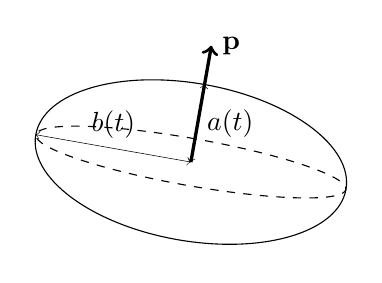
\begin{tikzpicture}[rotate=80]
        \draw(0,0) ellipse (1 cm and 2 cm);
        \draw[dashed](0,0) ellipse (0.3 cm and 2 cm);
        \draw[<->,very thin](0,0) --++ (1,0)node[midway,right]{$a(t)$};
        \draw[->,very thick](0,0) --++ (1.5,0)node[right]{$\textbf{p}$};
        \draw[<->,very thin](0,0) --++ (0,2)node[midway,above]{$b(t)$};
    \end{tikzpicture}
    \hfill
    \caption{Scheme of an  oblate spheroid oriented along the unit vector \textbf{p}.}
    \label{fig:scheme2}
\end{figure}
We consider in this problem an oblate spheroid with a time dependent aspect ratio $\chi = a(t)/b(t)$ oriented along the unit vector \textbf{p}, see \ref{fig:scheme2}.
We consider a mono disperse suspension of droplet with constant mass. 
The objective of this section is to derive constitutive equations to predict the mean orientation, and mean aspect ratio of the droplet. 

\subsubsection{Particle's internal motion}

In the first place we assume a linear homogeneous particle internal motion, such as, 
\begin{equation}
    \textbf{w}_2^0(\textbf{x}_\alpha+ \textbf{r})
    = 
    + \textbf{r} \cdot \textbf{D}_\alpha
    = 
    \bm{\omega}_\alpha \times \textbf{r} 
    + \textbf{r} \cdot \textbf{e}_\alpha
\end{equation}
where $\bm{\omega}_\alpha$ is the angular velocity of the particle, $\textbf{e}_\alpha$ is the mean deformation gradient. 
% Note that the second rank tensor $\textbf{U}_\alpha = \bm{\}$
To respect the mass conservation condition, i.e. $\div \textbf{w}_2^0 =0$, The mean gradient deformation $\textbf{e}_\alpha$ has to respect the conditions : $\textbf{e}_\alpha:\textbf{I}=0$. 
The assumption of linear internal motion is wrong for droplets and bubbles were we are clearly in presence of internal motions. 
However, for now these motions will be discarded. 

\subsubsection{Fundamental properties}

We now compute the mass, moment of mass and moment of momentum of this particle. 
The volume of an ellipsoid reads as, 
\begin{align}
    v_\alpha
    = \frac{4}{3}\pi a b^2
    = \frac{4}{3}\pi \chi  b^3
    \label{eq:volume_def}
\end{align}
Before going further we must say that the two radius $a(t)$ and $b(t)$ are actually dependent since one must preserve the total mass of the particle. 
We recall that we are in the context of mono disperse suspension such that the volume of the particles $v_\alpha$ is actually known, Thus, 
\begin{equation*}
    a(t) 
    = \frac{3 v_\alpha}{4 \pi b^2(t)}
    = \frac{r_0^3}{ b^2(t)}
    \Leftrightarrow
    b^2(t) 
    = \frac{r_0^3}{ a(t)}
\end{equation*}
Where $r_0$ is the radius of the sphere of same volume such as $v_\alpha = \frac{4}{3}\pi r_0^3$. 
Also, it might be useful to compute the relation between the derivative of the radius,  
\begin{equation*}
    \ddt v_\alpha 
    % = \ddt \frac{4}{3}\pi a b^2
    = \frac{4}{3}\pi \dot{a}(t) b^2(t)
    + \frac{8}{3} \pi {a}(t) b(t) \dot{b}(t)
    = 0 
    \Leftrightarrow
     \dot{a}(t)
    =  
    - 2 \frac{a(t)}{b(t)}  \dot{b}(t)
    % \Leftrightarrow
\end{equation*}
Which means that the derivative of both radius are related to twice the aspect ratio. 

The second moment of mass is somewhat more complicated to compute, we have, 
\begin{align*}
    \mathcal{M}_{\alpha,ij}
    = \int r_ir_j dxdydz
\end{align*}
At this stage we would like to compute the integral in spherical coordinate, thus we introduce the change of variables, 
\begin{align*}
    x' = x/a 
    && y' = y/b 
    && z' = z/b 
\end{align*}
By assuming that the spheroid is aligned with the $z$ axis and centered at the origin we get, 
\begin{align*}
    \mathcal{M}_{\alpha,zz}
    = a(t)^3 b(t)^2 \int z'z' dx'dy'dz'
\end{align*}
switching in spherical coordinate yields 
\begin{align*}
    \mathcal{M}_{\alpha,zz}
    = a(t)^3 b(t)^2 \int_0^1 \int_0^{2\pi}\int_0^\pi r^4 \cos^2\phi \sin\phi d\phi d\theta dr
    = a(t)^3 b(t)^2 \frac{1}{5}\frac{4}{3} \pi
    = v_\alpha \frac{a^2(t)}{5}\\
    \mathcal{M}_{\alpha,xx}
    = a(t) b(t)^4 \int_0^1 \int_0^{2\pi}\int_0^\pi r^4 \sin^3\phi\cos^2\theta d\phi d\theta dr
    = a(t) b(t)^4
    \frac{1}{5}
     \frac{4}{3}
     \pi
     =v_\alpha \frac{b^2(t)}{5}
\end{align*}
In a more general manner one can define the tensor $\mathcal{M}_\alpha$ in the laboratory reference frame using the orientation tensor \textbf{p}, such that, 
\begin{equation}
    5 \frac{\mathcal{M}_{\alpha,ij}}{v_\alpha}
    = p_i p_j 
    a^2(t) 
    + (\delta_{ij} - p_ip_j) b^2(t)
    = H_{ij}^{-1}
    \label{eq:M_alpha_def}
\end{equation} 
In light of \ref{eq:M_alpha_def}we reduced the description of any particle in our flow to four parameters, the 3 components of \textbf{p}, and the radius $a(t)$. 


Now let's compute the first moment of momentum $\mathcal{P}_\alpha$, it reads, 
\begin{align*}
    \mathcal{P}_{\alpha,ij}
    = \int r_i w_{2,j}^0 d\Omega
    = D_{\alpha,jk} \mathcal{M}_{\alpha,ki}
    = \epsilon_{jkl} \omega_{\alpha,k} \mathcal{M}_{\alpha,il}
    +  e_{\alpha,jk} \mathcal{M}_{\alpha,ik}
\end{align*}
Taking the double contracted product with $\epsilon_{mij}$ of the moment of momentum yield the angular momentum equation, 
\begin{align*}
    \mu_{\alpha,m}
    = \epsilon_{mij}\mathcal{P}_{\alpha,ij}
    = \epsilon_{jmi} \epsilon_{jkl} \omega_{\alpha,k} \int r_i r_l  d\Omega
    +  \epsilon_{mij} e_{\alpha,jk} \int r_i r_k  d\Omega\\
    = (\delta_{mk}\mathcal{M}_{\alpha,ll} - \mathcal{M}_{\alpha,mk}) \omega_{\alpha,k}
    +  \epsilon_{mij} e_{\alpha,jk} \int r_i r_k  d\Omega\\
    = \mathcal{I}_{\alpha,mk} \omega_{\alpha,k}
    +  \epsilon_{mij} e_{\alpha,jk} \mathcal{M}_{\alpha,ik}\\
\end{align*}
The second contribution of the angular momentum would vanish if the particles where spherical. 
Lastly, the symmetric part of the moment of momentum reads, 
\begin{align*}
    2\mathcal{S}_{\alpha,ij}
    = \epsilon_{jkl} \omega_{\alpha,k} \mathcal{M}_{\alpha,il}
    + \epsilon_{ikl} \omega_{\alpha,k} \mathcal{M}_{\alpha,jl}
    +  e_{\alpha,jk} \mathcal{M}_{\alpha,ik}
    +  e_{\alpha,ik}  \mathcal{M}_{\alpha,jk}
\end{align*}

\subsubsection*{Evolution equation of a single particle shpae.}

We first start by the kinetic equations.  
In view of the previous expression the evolution equation of the momentum tensor is,  
\begin{equation*}
    \ddt \mathcal{M}_{\alpha,ij}
    + \epsilon_{jlk} \omega_{\alpha,k} \mathcal{M}_{\alpha,il}
    - \epsilon_{ikl} \omega_{\alpha,k} \mathcal{M}_{\alpha,jl}
     =  e_{\alpha,jk} \mathcal{M}_{\alpha,ik}
     +  e_{\alpha,ik}  \mathcal{M}_{\alpha,jk}
     \label{eq:dt_M_alpha_bis}
\end{equation*}
On the left-hands-side of \ref{eq:dt_M_alpha_bis} we clearly identify the Jaumann derivative rotating with the vorticity.
To close this equation one may relate the mean ambient flow variables to the particles angular rotation and stretching rate. 
This however this is only possible considering pure stokes flow.

\subsubsection*{Equation for the bulk stress}

The equivalent stress can be formulated as, 
\begin{equation*}
    \bm{\sigma}
    = 
    \phi_1 \bm{\sigma}_1
    + \phi_2 \bm{\sigma}_2
    + \phi_I \bm{\sigma}_I
    \label{eq:sigma_def}
\end{equation*}
The particle phase stress can be reduced to its first moment, $\phi_2 \bm{\sigma_2} = \pOavg{\bm{\sigma}_2^0}$ and thus, 
\begin{equation*}
    \phi_2 \bm{\sigma}_2 
    = - \phi_2 p_2
    + \phi_2 \mu_2 \textbf{e}_p 
\end{equation*}
Using the following expression for $\phi_1 \bm{\sigma}_1 = - \phi_1 p_1 + \mu_1 \phi_1 \textbf{e}_1 =  - \phi_1 p_1 + \mu_1 \textbf{e} - \mu_1 \phi_2 \textbf{e}_2$.
Likewise since we considered a constant strain within the particle we can write $\phi_2\textbf{e}_2 = \phi_2 \textbf{e}_p$ in homogeneous medium.   
The previous expression of the averaged stress yields, 
\begin{equation*}
    \bm{\sigma}
    = 
    - p 
    + \mu_1 \textbf{e} 
    + (\mu_2 - \mu_1) \phi_2 \textbf{e}_2
    + \phi_I \bm{\sigma}_I
    \label{eq:sigma_def}
\end{equation*}
In the above stress equation $\bm{\sigma}_I$ is unknown and must be closed. 
While the others parameters can be easily linked to our problem variable. 

We recall that in homogeneous flows, $\phi_I \bm{\sigma}_I = \gamma\pSavg{\textbf{I}-\textbf{nn}}$. 
Therefore, to close this term one must compute the curvature of the particles. 
The first moment of surface tension stress can be computed analytically following \citep{nadim1996concise} for the curvature computation.
In this context an equation describing the droplets surface can be found in the reference frame of the droplets, namely, 
\begin{equation}
    \mathscr{F}
    = \textbf{r}\cdot \textbf{H}\cdot \textbf{r} - 1 = 0 
    \label{eq:F_def}
\end{equation}
where \textbf{H} is a symmetric traceless tensor such that $\textbf{H} = \textbf{pp}/a^2(t) + (\textbf{I}- \textbf{pp})/b^2(t)$. 
This analytical expression will enable us to compute the curvature of each particle.  
Let $\mathscr{F}(\textbf{x},t) = 0$ be the equality representing the ellipsoidal shape of the particle. 
First, the normal pointing in the direction of positive $\mathscr{F}$ at the interface, can be computed as, 
\begin{equation*}
    \textbf{n} = \frac{\grad \mathscr{F}}{(\grad \mathscr{F}\cdot \grad \mathscr{F})^{1/2}} \;\;\text{ on }\;\; \mathscr{F} = 0.  
\end{equation*}
It follows that the local surface stress is, 
\begin{equation*}
    \bm{\sigma}_I^0 =
    \gamma \left[\textbf{I} - \frac{\grad \mathscr{F} \grad \mathscr{F}}{\grad \mathscr{F}\cdot \grad \mathscr{F}}\right] \;\;\text{ on }\;\; \mathscr{F} = 0.  
\end{equation*}
Noticing that $\grad \mathscr{F} = 2\textbf{H}\cdot \textbf{r}$ one obtain, 
\begin{equation*}
    \bm{\sigma}_I^0 =\gamma\left[
    \textbf{I} - \frac{ \textbf{HH} :  \textbf{rr}}{ (\textbf{H}\cdot  \textbf{H}\cdot \textbf{rr})} \right]
\end{equation*}
In indices notation,  
\begin{equation*}
    \sigma_{I,ij}^0 =\gamma\left[
    \delta_{ij} - \frac{ H_{ik} H_{jl} :  r_kr_l}{  H_{ab}  H_{ac} r_br_c} \right]
\end{equation*}
Integrating this over a surface will eventually leads to an elliptic integral due to the elliptical surface. 
\subsubsection*{Equation for the particles strain}

Additionally, using the first moment of momentum expression one can obtain an other expression for the particles internal stress, 
\begin{equation}
    \intS{ (\bm{\sigma}_I)_{ik}}
    +\intO{ (\bm{\sigma}_2^0)_{ik}}
    = 
    \intO{ \rho_2 
    (\textbf{w}_2^0\textbf{w}_2^0  )_{ik}
    }
    -\ddt \intO{ r_i (\textbf{u}^0_2)_k }
    +\intS{ 
     r_i (\bm{\sigma}_1^0 \cdot \textbf{n}_2)_{k}
    }
\end{equation}
\subsection{Equation for the particle angular momentum}
\begin{equation*}
    \ddt \mu_p = t_p
\end{equation*}
% \input{Closure_hybrid/Fluid_phase_eq.tex}

% 

The conservation equations of mass and momentum, derived using \ref{eq:avg_dt_dq_alpha_tot} and \ref{eq:hybrid_avg_dt_chif} yield the same as the classical hybrid models derived in previous studies such as \citet{jackson1997locally} and \citet{zhang1997momentum} among others.
Therefore, it will not be discussed further as it does not contribute any relevant information to the current study.
Instead, in the subsequent analysis, we consider as known quantities : the fluid phase fraction $\phi_1$;
the particle number density $n_p$; the continuous phase-averaged velocity $\oneavg{\textbf{u}}$; and particle-average velocity $\pnnavg{\textbf{u}_\alpha}$. 
Which implies that the equations of conservation of mass and momentum for both the continuous and dispersed phase have been solved a priori, providing the values of these variables as known quantities.
Additionally, it also implies that the closure terms in the momentum equation, such as the mean interphase drag force $\pnnavg{\textbf{f}_\alpha}$ and others terms must be closed. 
However, those terms might depend on the higher moments of the particle phase, in which case it is crucial to provide a first-order moment equation. 
Therefore, the primary objective of this section is to emphasize the significance of the first-moment equations derived from \ref{eq:avg_dt_dQ_alpha_tot}, as they are often overlooked and underutilized in the literature.
In this section we stay succinct while providing the minimum level of understanding of the problem at hand.
Hence, we will not entirely deal with the closure problem of these first-order moments equations, but rather we focus on their derivation and interpretation. 

\subsection{Solid axis symmetric particle suspension}

% Let's start by the second moment of mass averaged equation.
Let's examine the scenario of a mono-disperse axissymmetric suspension of solid particles, such as ellipsoid or cylinders.
Let the vector $\textbf{p}$ denote the unit vector representing the orientation of the particle along its main axis of inertia. 
Then, the second moment of mass can be written as $\mathcal{M}_\alpha =  \textbf{pp} (M_\alpha^{||} - M_\alpha^\bot) +  \textbf{I} M_\alpha^\bot$, where $M_{\bot}$ and $M_{||}$ represent the coefficients corresponding to the principal directions of the particles' mass distribution.
It is well-established that $\pnnavg{\textbf{f}_\alpha}$ exhibits a significant dependence on the orientation of the particle \citep{kim2013microhydrodynamics}.
Therefore, despite being a second-order moment, the particle field $\mathcal{M}_\alpha$ is indispensable to solve the mono-disperse axissymmetric suspension problem.

Averaging the second-order moment of mass yields, $\pnavg{\mathcal{M}_\alpha} =  \textbf{A} (M_\alpha^{||} - M_\alpha^\bot) +  \textbf{I} M_\alpha^\bot$ where $\textbf{A}$ is the orientation tensor defined as $\textbf{A} = \avg{\delta_\alpha\textbf{pp}} = \pnavg{\textbf{pp}}$.
Then, let's express the internal motion of a solid particle by : $\textbf{u}_2(\textbf{x}_\alpha) = \textbf{u}_\alpha + \textbf{r}\times \omega_\alpha$ where $\omega_\alpha$ represents the angular velocity of the particle.
It follows the expression of the stretching of momentum : $\mathcal{S}_\alpha = (M_\alpha^{||} - M_\alpha^\bot) \left(
    \omega_\alpha \times
    \textbf{pp}
    + \textbf{pp} \times \omega_\alpha
\right)$. 
Subsequently,  we can easily derive the transport equation for $\textbf{A}$ by averaging \ref{eq:dt_M_alpha} and using the previous expressions for $\mathcal{M}_\alpha$ and $\mathcal{S}_\alpha$.
The resulting equation is given by~:
\begin{equation}
    \pddt (n_p\textbf{A})
    + \div (
        \pnnavg{\textbf{u}_\alpha}\textbf{A}
        + \mathbf{\Sigma}
        )
    =
    \pnavg{\textbf{pp} \times \omega_\alpha}
    + \pnavg{\omega_\alpha \times \textbf{pp}},
    % + \pnavg{\textbf{pp}' \times \omega_\alpha'}
    % +\pnavg{\omega_\alpha' \times \textbf{pp}'}
    \label{eq:avg_dt_M_alpha}
\end{equation}
where $\mathbf{\Sigma} = \pnavg{\textbf{u}'_\alpha(\textbf{pp})'}$ is the covariance term between the fluctuation of the velocity and the orientation tensor.
We recall that the definition of the fluctuation notation is provided by the expression from \ref{eq:def_fluctu}.
At this stage we need to find closure for both terms on the RHS of \ref{eq:avg_dt_M_alpha}. 
Therefore, we assume torque free rigid particle in to Stokes flow, where we can utilize Jeffery's equation \citep{guazzelli2011}.
It reads,
\begin{equation}
    \omega_\alpha \times \textbf{p}
    = \mathbf{\Omega}\cdot\textbf{p}
    + \beta\left(
        \textbf{E}\cdot \textbf{p}
        - \textbf{E} : \textbf{ppp}
    \right),
    \label{eq:jefferey}
\end{equation}
with $\textbf{E}$ and $\mathbf{\Omega}$ being the symmetric and antisymmetric parts of the bulk velocity gradient, respectively, such that $\grad\avg{\textbf{u}}=\textbf{E}+\mathbf{\Omega}$.
The coefficient $\beta$  is a constant related to the aspect ratio of the particle.
Finally, by substituting the RHS terms of \ref{eq:avg_dt_M_alpha}, by using \ref{eq:jefferey}, we arrive at the closed form of the second moment of mass equation~:
\begin{equation}
    \pddt \textbf{A}
    + \div (
        \pnnavg{\textbf{u}_\alpha}\textbf{A}
    )
    =
    \mathbf{\Omega} \cdot \textbf{A}
    - \textbf{A} \cdot \mathbf{\Omega}
    + \beta\left[
        \textbf{E} \cdot \textbf{A}
        -\textbf{A} \cdot \textbf{E}
        - \textbf{E} : \mathbb{A}
    \right]
    - \div \mathbf{\Sigma}
    \label{eq:hybrid_avg_dt_pp}
\end{equation}
where the fourth-order tensor $\mathbb{A}$, is defined as $\mathbb{A} = \pnavg{\textbf{pppp}}$.
In \citet{wang2008objective} they derive \ref{eq:hybrid_avg_dt_pp} by the means of kinetic theory, based on \ref{eq:jefferey} and the fact that $\ddt \textbf{p} = \omega_\alpha \times \textbf{p}$ (Equation (3) of their article).
Their equation is similar to \ref{eq:hybrid_avg_dt_pp} except that their employ a phenomenological closure for the term, $\div \mathbf{\Sigma}$, which account for particles interactions.
Anyhow, we showed how it is possible to derive the orientation tensor conservation equation, commonly used in fiber field theory, from the second-order moments of mass's equation. 

\subsection{Contaminated bubbly flows}

Let's consider a mono-disperse rising bubbly flow without phase transfer made of spherical particles of radius $a$, that is contaminated by soluble surfactants.
We denote $c_1$ as the molar concentration of surfactant in the continuous phase, and $c_I$ as the surface molar concentration of surfactant on the bubbles' interface.
Additionally, we make the assumption that there is no transport of surfactant inside the dispersed phase. 
This assumption is reasonable in the case of air bubbles.
According to the Langmuir model \citep{pesci2018computational}, we have the relationship:
\begin{equation}
    \sigma
    = \sigma_0
    + RT c_I^\infty
    \ln\left(1-\frac{c_I}{c_I^\infty}\right)
    \label{eq:sigma_def}
\end{equation}
where $R$ is the universal gas constant, $T$ the absolute temperature, $c_I^\infty$ the saturated surfactant concentration, and $\sigma_0$ to the surface tension coefficient when the surfaces are completely clean.
On the other hand, as represented on \ref{fig:contaminated_bubbles}, during the rise of a bubble in the flow, the surfactants are transported along the droplets surface, which in turns create a stagnant cap in the opposite direction of the droplet velocity.
According to \ref{eq:sigma_def} the possibly inhomogeneous concentration field, $c_I$, generates a spatially non-constant surface tension coefficient $\sigma$.
Additionally, remark that the gradient of the surface tension generates additional Marangoni forces as represented in \ref{fig:contaminated_bubbles} and expressed by \ref{eq:surface_tension}.
These additional surface tension forces alter the flow behavior in the vicinity of the droplet's surface.
Therefore, this alteration in surface tension impacts the local hydrodynamic, but also induce a change in the shape of the particle through both, \ref{eq:dt_S_alpha} and \ref{eq:dt_M_alpha}.
As a result, the drag force and drift velocity experienced by a rising bubble or droplet are directly influenced by the surfactant concentration and its distribution over the surface \citep{pesci2018computational}.
Moreover, a recent study by \citet{kentheswaran2022direct} have demonstrated that the mean concentration and distribution of surfactants on the bubbles' surface also have a significant impact on the mass transfer rate between the dispersed and continuous phases.
Therefore, in this example we present an averaged hybrid model that aims to predict the evolution of the averaged surfactant concentration in the bulk $\oneavg{c}$, and the averaged surfactant on the surface of the particle, defined by, $C_{\alpha}= \frac{1}{s_\alpha}\int c_I d\Sigma$.
Additionally, we also provide the moment equation for the center of the distribution of $c_I$, which is defined as $\textbf{r}_\alpha = \frac{1}{s_\alpha C_\alpha}\int_{\Sigma_\alpha} \textbf{r}c_Id\Sigma$.
Note that $\int_{\Sigma_\alpha} \textbf{r}c_Id\Sigma =  \frac{s_\alpha}{4 \pi}\int_{\Sigma_\alpha} \gradI (c_I) d\Sigma$, thus $\textbf{r}_\alpha$ can also be interpreted as the mean gradient of surfactant on a particle's surface.
Consequently, by the mean of \ref{eq:sigma_def}, $\textbf{r}_\alpha$ is also related to the resultant of Marangonie forces on a particle's surface.  
A graphical representation of $\textbf{r}_\alpha$ is given \ref{fig:contaminated_bubbles}.

\begin{figure}[h!]
    \centering
    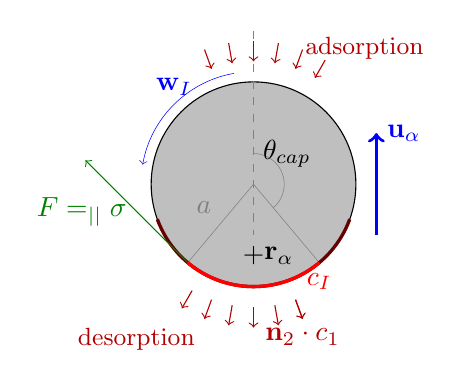
\begin{tikzpicture}[scale =1.3]
        \draw[fill=lightgray](0,0) circle (1);
        \draw[very thin,gray](230:1)--(0,0)node[midway,above left]{$a$}--(310:1);
        \draw[very thin,gray](0,0)++(310:0.3) arc (-50:90:0.3)node[right,black]{$\theta_\text{cap}$};
        \draw[very thin,blue,->](0,0)++(100:1.1) arc (100:170:1.1)node[midway,above]{$\textbf{w}_I$};
        \draw[very thick,red!40!black](0,0)++(200:1) arc (200:340:1);
        \draw[very thick,red](0,0)++(230:1) arc (230:310:1)node[below]{$c_I$};
        \draw[very thick,dashed](0,0)++(0,-0.7)node{$+$}node[right]{$\textbf{r}_\alpha$};
        \draw[very thick,blue,->](1.2,-0.5)--++(0,1)node[right]{$\textbf{u}_\alpha$};
        \draw[dashed,gray](0,1.5)--++(0,-2);
        \draw[red,->,green!50!black](230:1)--++(-1,1)node[midway,left]{$F = \grad_{||} \sigma$};
        \foreach \t in {110,100,90,80,60}{
            \draw[red!70!black, ->](\t:1.4)--++(\t:-0.2);
            \draw[red!70!black, ->](\t:-1.2)--++(\t:-0.2);
        }
        \draw[red!70!black, ->](70:1.4)--++(70:-0.2)node[above right]{\small adsorption};
        \draw[red!70!black, ->](70:-1.2)--++(70:-0.2)node[below left]{\small desorption};
        \draw[red!70!black, ->](110:-1.2)--++(110:-0.2)node[below]{$\textbf{n}_2 \cdot \grad c_1$};
    \end{tikzpicture}
    \hspace{2em}
    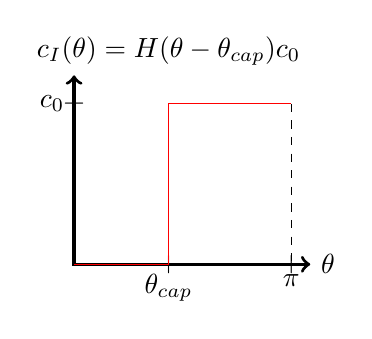
\begin{tikzpicture}[scale =1.2]
        \draw[very thick,<->](0,2)--(0,0)--(2.5,0)node[right]{$\theta$};
        \draw(1,0)node{$+$}node[below]{$\theta_{cap}$};
        \draw(1,2)node[above]{$c_I(\theta) = H(\theta- \theta_{cap}) c_0$};
        \draw[very thin,dashed](2.3,1.7)--(2.3,0);
        \draw[thin,red](0,0)--++(1,0)--++(0,1.7)--++(1.3,0);
        \draw(2.3,0)node{$+$}node[below]{$\pi$};
        \draw(0,1.7)node{$+$}node[left]{$c_0$};
    \end{tikzpicture}
    \caption{ (left) Scheme of the stagnant-cap regime of a rising contaminated bubble in a quiescent liquid. 
    (right) Hypothetical profile of the surface concentration $c_I$ in terms of the azimuthal coordinate $\theta$. }
    \label{fig:contaminated_bubbles}
\end{figure}


To derive the microscopic scale conservation equation of $c_I$ and $c_1$ we set $f_1 = c_1$ and $f_I = c_I$ in \ref{eq:dt_f_k} and \ref{eq:dt_f_I}, respectively.
Additionally, we assume that the  diffusive flux follow a Fick's law model, i.e.  $\mathbf{\Phi}_1 = D\grad c_1$ and $\mathbf{\Phi}_I = D_I\gradI c_I$,
where the constant,  $D$ and $D_I$ are the volumetric and surface diffusion coefficient, respectively.
Note that this diffusive model remains true under the assumption of dilute species concentration in both the liquid and at the interface.
\tb{The diffusive terms change in function of the regime : dilute concentration / saturated concentration, in which case $D\grad c_1 = f(c_I)$, it is worth going into that mush details ? no.}
Moreoverer, We do not consider chemical reaction or any other source term, i.e. $\textbf{S}_k = 0$ and $\textbf{S}_I=0$. 
Then, by injecting these terms in \ref{eq:dt_f_k} and \ref{eq:dt_f_I} we obtain these conservation equations : 
\begin{align}
    \pddt c_1
    + \div (\textbf{u}_1 c_1)
    &= \div (D \grad c_1)
    \;\;\; \text{in} \;\;\; \Omega_1,\\
    \pddt c_I
    + \divI (\textbf{u}_I c_I)
    &= \divI (D_I \gradI c_I)
    - (D \grad c_1)\cdot \textbf{n}_2
    \;\;\; \text{on} \;\;\; \Sigma,
    \label{eq:dt_c_I}
\end{align}
In agreement with \citet{pesci2018computational,manikantan2020surfactant}.
We recognize that the last term of \ref{eq:dt_c_I}, namely $D(\grad c_1 ) \cdot \textbf{n}_2$, turns out to be the \textit{Kinetically controlled sorption} boundary condition \citet{pesci2018computational,manikantan2020surfactant} which arise naturally in our model.
Specifically, it represents the adsorption and desorption flux between the bulk and the surface, as represented in \ref{fig:contaminated_bubbles}.
% For clarity remark that for exemple Equation (3.9) of \citet{manikantan2020surfactant} corresponds to the \textit{two-fluid} formulation of \ref{eq:dt_c_I} with a Fick's law model. 
Note that this exchange term is reduced to a contribution from the continuous phase since we assume no surfactant into the dispersed phase. 
Now that we clearly derived the microscale equation in both phases, we can easily derive the averaged equations of conservation using the hybrid model presented \ref{sec:averaged_eq}.

For a better understanding of the following equations, we now describe the steady-state kinetics that can be reached for an isolated bubble in a contaminated flow, as illustrated on \ref{fig:contaminated_bubbles}.
This will serve as a reference for the subsequent discussion.
We first assume that the transport of surfactants on the surface, represented  by the term  $\textbf{w}_I c_I$, is much greater than the other diffusive processes, such as $D\grad c_1$ and $D_I\gradI c_I$ as well as the adsorption-desorption effects. 
In this regime, the concentration of surfactant that enters from the forward-surface, due to adsorption, is advected almost instantaneously to the downward region of the particle where some of it evaporates due to desorption. 
This form an accumulation of surfactant on the downward region of the particle's surface.
At a certain point of equilibrium, the adsorption and desorption flux balance each other, leading to the steady-state kinetic of $c_I$, and the stagnant cap is stabilized to a concentration $c_0$. 
In this situation, we can consider that $c_I$ follows a constant sharp distribution along the azimuthal coordinate of the particle's surface.
Specifically, we model $c_I(\theta) = H(\theta - \theta_{cap}) c_0$ where $H$ is the Heaviside function and $\theta_{cap}$ is the angle at which the stagnant cap is formed, see \ref{fig:contaminated_bubbles}.
This assumption might seem unrealistic, nevertheless in the steady-state regime, it is approximately consistent with the observations \citep{kentheswaran2022direct}.
% In these condition the physical meaning of the first moment, $\textbf{r}_\alpha$, becomes clearer. 
From the expression of $c_I$ we deduce : $C_\alpha = \frac{c_0}{2}(1+\cos\theta_{cap})$ and $\textbf{r}_\alpha = \frac{a}{2} (\cos\theta_{cap} -1)\textbf{e}$ where $\textbf{e}$ is the unit vector in the direction of the relative velocity between the particle and the continuous phase velocity.
Thus, the knowing $\textbf{r}_\alpha$ can leads use to $\theta_{cap}$. 
This is crucial information, since the drag forces term and mass transfer closure terms are usually derived in terms of $\theta_{cap}$, such as in the following studies : \citet{sadhal1983stokes} and \citet{kentheswaran2022direct}. 

Now that the problem has been properly formulated, we can begin the derivation of the averaged equations.
The phase-averaged conservation equation for the mean concentration of surfactant in the bulk $\oneavg{c}$, is derived using \ref{eq:avg_dt_chi_f}.
It reads as,
\begin{equation}
    \pddt (\phi_1 \oneavg{c})
    + \div (\phi_1 \oneavg{c} \oneavg{\textbf{u}_1})
    = D \grad^2 (\phi_1\oneavg{c})
    - \pnavg{j_\alpha}
    +  \div \mathbf{\Sigma}_c,
    \label{eq:hybrid_avg_dt_c_1}
\end{equation}
where $j_\alpha$ is the exchange term with the dispersed phase given by,
\begin{equation*}
    j_\alpha
    =\int_{\Sigma_\alpha}
    (D\grad c_1 )
\cdot \textbf{n}_2d\Sigma,
\end{equation*}
which corresponds to the resultant of the surfactant exchange including adsorption and desorption flux.  
In the steady-state regime, when the adsorption flux balance the desorption flux,  the surfactant on the surface of the bubble can be considered as globally insoluble since $j_\alpha=0$ even through $D(\grad c_1 ) \cdot \textbf{n}_2$ may not be locally zero. 
This \textit{globally insoluble} assumption has been used in numerous studies to neglect the adsorption-desorption fluxes. 
The vector $\mathbf{\Sigma}_c$ in \ref{eq:hybrid_avg_dt_c_1}, has the following expression,
\begin{equation}
    \mathbf{\Sigma}_c
    =
     \pnavg{\textbf{J}_\alpha}
    - \pnavg{\frac{D}{a}\int_{\Sigma_\alpha}  c_1 \textbf{r} d\Sigma}
    - \phi_1\oneavg{c'_1\textbf{u}_1'},
    \label{eq:B_def}
\end{equation}
where the higher order terms have been neglected. 
The first term on the RHS of \ref{eq:B_def} corresponds to the first moment of the surfactant flux, namely $\textbf{J}_\alpha = \int_{\Sigma_\alpha} \textbf{r}
(D\grad c_1)\cdot \textbf{n}_2d\Sigma$.
It can be interpreted as the vector representing the mean direction and magnitude of the surfactant flux going in and out the surface of the droplets.
In the stagnant cap regime, this term is therefore non-zero since a mean flux is still present even through its resultant is null, i.e. $j_\alpha=0$.
In the reference frame of the particles, $\textbf{J}_\alpha$ account for the mean flux of species concentration induced by the presence of the particles, due to adsorption and desorption phenomena. 
The second term of \ref{eq:B_def} comes from the inclusion of $\phi_1$ inside the Laplacian operator in \ref{eq:hybrid_avg_dt_c_1}.
It is the first moment of $c_1$ over the droplets surface, thus it is the mean position of the continuous phase surfactant concentration over the droplet surface.
For a constant distribution $c_1$ at the bubbles interface, this vector would be zero. 
Finally, The last term of \ref{eq:B_def}, $\phi_1\oneavg{c'_1\textbf{u}_1'}$, represents the diffusive term due to the correlation of $c'_1$ with $\textbf{u}_1'$.
Overall, $\mathbf{\Sigma}_c$ is a balance between the first moment of the fluxes and the first moment of the bulk concentration, minus a contribution from the fluctuations.
Note that $\mathbf{\Sigma}_c$ appear under the divergence operator in \ref{eq:hybrid_avg_dt_c_1}, thus it will be relevant only in highly inhomogeneous cases. 
% At this stage of the research it is hard to predict the form of these closure terms. 
% Nevertheless, we know that the closure for $j_\alpha$ and $\mathbf{\Sigma}_c$ are function of the mean surface concentration $C_\alpha$ and its center of distribution $\textbf{r}_\alpha$.
% Indeed, the exchange term $\grad c_1$ which is function of the local concentration $c_I$ at surfactant saturation \citep{manikantan2020surfactant}. 
% Thus, an equation for $C_\alpha$ and a moment equation for $\textbf{r}_\alpha$ are needed. 

Regarding the equations dispersed phase, we start by the transport equation of the mean surface surfactant concentration $C_\alpha$.
From \ref{eq:avg_dt_dq_alpha_tot} the averaged conservation equation of $C_\alpha$ is straightforward to obtain and reads as,
\begin{equation}
    \pddt (\pnavg{C_\alpha})
    + \div (\pnavg{\textbf{u}_\alpha} \pnnavg{C_\alpha})
    =
    \frac{\pnavg{j_\alpha}}{s_\alpha}
    - \div (\pnavg{\textbf{u}_\alpha' C'_\alpha}).
    \label{eq:avg_dt_dC_alpha}
\end{equation}
As shown by this equation, the evolution of the mean concentration of surfactant on the particles' surface is driven by the exchange term $j_\alpha$ and the fluctuation term $\pnnavg{\textbf{u}_\alpha' C_\alpha'}$. 
The latter term is the covariance between the velocity of the particles and their mean surfactant concentration. 
It is known that the rising velocity of a bubble is greatly correlated with its mean surfactant concentration \citet{kentheswaran2022direct} thus it might be of a certain importance. 
Again, this term is under the divergence operator it will be therefore important only in non-homogeneous cases. 
Anyhow, this term must be further investigated.

We now derive an equation for the mean position of the surfactant, $\pnnavg{\textbf{r}_\alpha}$.
This is done by deriving the equation of the first moment, $s_\alpha C_\alpha \textbf{r}_\alpha$ using \ref{eq:dt_Q_alpha_tot}. 
Then, we reformulate the equation using  the relation, $\ddt (s_\alpha C_\alpha \textbf{r}_\alpha) = s_\alpha C_\alpha\ddt \textbf{r}_\alpha+ s_\alpha \textbf{r}_\alpha\ddt C_\alpha $ and  $\ddt C_\alpha = j_\alpha$. 
Finally,  we apply the average process which leads us to~:
\begin{multline}
    \pddt (\pnavg{\textbf{r}_\alpha})
    + \div (\pnavg{\textbf{u}_\alpha}\pnnavg{\textbf{r}_\alpha})
    =
    - \div (\pnavg{\textbf{u}'_\alpha\textbf{r}'_c})\\
    + \frac{n_p}{s_\alpha}\pnnavg{
        \frac{1}{C_\alpha}\left[
            \int_{\Sigma_\alpha} 
            \left[
                c_I \textbf{w}_I
                - D_I (\gradI c_I)
            \right] d\Sigma
            +\textbf{J}_\alpha
            - \textbf{r}_\alpha j_\alpha
        \right]
    }.
    \label{eq:avg_dt_dr_alpha_tot}
\end{multline}
The diffusive term $\pnavg{\textbf{u}'_\alpha\textbf{r}'_c}$ which represents the flux generated by the correlation between the mean surfactant distribution on the particles' surface and the velocity of the particles. 
Again, this term might be relevant since, as mentioned previously, the rising velocity is highly dependent on $\theta_{cap}$.
Then, the first term on the second line is the contribution of the averaged surface advection of $c_I$ along the particles' surface. 
The second term accounts for the diffusion of surfactants over the droplet surface, which acts against the formation of a sharp distribution of surfactants.
However, the contribution of this term is likely negligible based on the values of the diffusive surface coefficient, as discussed in \citet{valkovska2000determination}.
The third term of the second line, is the exchange term $\textbf{J}_\alpha$ which clearly impacts $\textbf{r}_\alpha$.
Indeed, this term accounts for the inward adsorption of concentration and downward desorption fluxes of surfactant, creating a significant disequilibrium. 
The last term, $\textbf{r}_\alpha j_\alpha$, is the contribution from the accumulation of species adsorption and desorption on the particle surface during the process driven by the three previous terms, i.e. adsorption, advection, diffusion and desorption. 
We may recognize that the latter fourth terms are being responsible for the equilibrium or not of the cap angle. 
Indeed, when all these terms are balanced, the system reaches a steady-state equilibrium for the surfactant distribution.
It is evident that in the closure of \ref{eq:avg_dt_dr_alpha_tot} one can include all properties linked to the physics of the bubbles' surface, which in turn creates a model for the surfactant distribution at first order. 

\tb{Dans cette partie il faut encore que je lise la bibliography qui existe peut etre sur ces dernière equaiton pour voir i le tout est bien coherent}

% \tb{Start : in the SSR the stagnat can is funciton of Re anfd Ma}
% Let assume that the timescale to reach the steady-state kinetic regime is much shorter than the variation of $\oneavg{c}$ seen by the particles. 
% In this situation the advection flux compensate the diffusive flux and adsorption-desorption source terms for all particles at all times.
% This equilibrium can be written :
% \begin{equation}
%     \int_{\Sigma_\alpha} 
%         c_I \textbf{w}_I
%         d\Sigma
%         - \int_{\Sigma_\alpha} 
%         D_I (\gradI c_I)
%          d\Sigma
%         +\textbf{J}_\alpha
%         = 0 
%         % - \textbf{r}_\alpha j_\alpha
%         \label{eq:steady_state_kinetic_regime}
% \end{equation}
% Nevertheless, due to a change of environment, $\oneavg{c}$ can change slowy inducing a non-zero $j_\alpha$, after what the particles reache instantaneously another steady-state kinetic regime. 
% In this situations the mean position of the surfactant is fully determined with the local concentration $\oneavg{c}$ or the local source $j_n$.
% Using the hypothesis \ref{eq:steady_state_kinetic_regime} in \ref{eq:avg_dt_dr_alpha_tot} gives the quasy steady conservation equaiton of $\textbf{r}_c$ with :
% \begin{equation}
%     \pddt (\pnavg{\textbf{r}_\alpha})
%     + \div (\pnavg{\textbf{u}_\alpha}\pnnavg{\textbf{r}_\alpha})
%     =
%     - \frac{n_p}{s_\alpha}\pnnavg{
%          \frac{\textbf{r}_\alpha j_\alpha}{C_\alpha}
%     }
%     - \div (\pnavg{\textbf{u}'_\alpha\textbf{r}'_c})
% \end{equation}
% where $\textbf{r}_\alpha$ is solely function on the local flux on the a the diffusive fluctuation term. 


As the objective of this study is not to provide a fully closed system, we will conclude the discussion on this point.
In short, this new system of equations can be used to determine the macroscopic variables $\pnnavg{C_\alpha}$ and $\pnnavg{\textbf{r}_\alpha}$, which are crucial for the closure of drag force and mass transfer in the macroscopic models.
Unfortunately, at the current state of the art, it is still challenging to derive exact closure terms for these equations, even in simplified regimes. 
However, we provided a clear methodology to derive a hybrid model tailored to the problem at hand, using the examples of surfactant transport and fiber suspension. 


% \section{Brouillion}
\subsection*{Fluid formulation meaningful exchange terms}


Using the generic formulation \ref{eq:hybrid_avg_dt_chif} and the local expression of the mass, momentum and total energy expression, i.e. : \ref{eq:dt_rho},\ref{eq:dt_rhou_1} and \ref{eq:dt_rhoE_1} we easily find the averaged form of these equations as, 

\begin{align}
    \pddt (\phi_1 \rho_1)  
    + \div (
        \phi_1 \rho_1\textbf{u}_1
    )
    &= 
    0\\
    \pddt (\phi_1 \rho_1\textbf{u}_1)  
    + \div (
        \phi_1 \rho_1\textbf{u}_1\textbf{u}_1
        + \bm{\sigma}_1^\text{eq}
    )
    &= 
    \phi_1 \rho_1 \textbf{g} 
    -  \avg{\delta_I \bm{\sigma}_1^0 \cdot \textbf{n}_2}\\
    \pddt (\phi_1\rho_1E_1)  
    + \div (
        \phi_1\rho_1E_1\textbf{u}_1
        + \bm{q}_1^\text{eq}
        + \textbf{u}_1 \cdot \bm{\sigma}_1^\text{eq}
        % - \textbf{u}_1^0 \cdot \bm{\sigma}_1^0 
        % + \textbf{q}_1^0
        )
    &= 
    \phi_1 \rho_1\textbf{u}_1 \cdot \textbf{g} 
    - \avg{\delta_I (\textbf{u}_1^0 \cdot \bm{\sigma}_1^0 - \textbf{q}_1^0)\cdot \textbf{n}_2}
\end{align} 
where we have defined, 
\begin{align*}
    &\bm{\sigma}_1^\text{eq}
    = \phi_1 (
        \rho_1\kavg{\textbf{u}_1'\textbf{u}_1'}
        - \bm{\sigma}_1%- n_p \textbf{M}_p
         )  
    &\textbf{q}_1^\text{eq}
    =\textbf{q}_1^\text{e} +\textbf{q}_1^\text{k}  \\
    &\textbf{q}_1^\text{e}
    = \phi_1\rho_1 \kavg{\textbf{u}_1' e_1'} 
    + \phi_1\textbf{q}_1 
    &\textbf{q}_1^\text{k}
    = \phi_1\rho_1 \kavg{\textbf{u}_1' k_1} 
    - \phi_1\kavg{\textbf{u}_1' \cdot \bm{\sigma}_1^0}
\end{align*}
Note that the phase averaged energy equation can be further decompose following, 
\begin{align*}
    E_1 = e_1 + k_1 + u_1^2/2
    \label{eq:E_def}
\end{align*}
where $K_1$ is the pseudo-turbulent kinetic energy defined such as, $\phi_1 k_1 = \avg{\chi_1 (u_1')^2/2}$. 
The Macroscopic kinetic energy equation can be obtain by taking the dot product with $\textbf{u}_1$. 
\begin{align}
    \pddt (\phi_1 \rho_1u_1^2/2)  
    + \div (
        \phi_1 \rho_1\textbf{u}_1u_1^2/2
        + \textbf{u}_1 \cdot \bm{\sigma}_1^\text{eq}
    )
    &= 
     \bm{\sigma}_1^\text{eq} : \grad \textbf{u}_1
    + \phi_1 \rho_1 \textbf{u}_1\cdot \textbf{g} 
    -  \textbf{u}_1\cdot \avg{\delta_I \bm{\sigma}_1^0 \cdot \textbf{n}_2}\\
    \pddt (\phi_1\rho_1k_1)  
    + \div (
        \phi_1\rho_1k_1\textbf{u}_1
        + \textbf{q}_1^\text{k} 
        )
    &= 
    - \avg{\chi_1\bm{\sigma}_1^0 : \grad \textbf{u}_1^0}
    - \bm{\sigma}_1^\text{eq} : \grad \textbf{u}_1
    - \avg{\delta_I \textbf{u}_1' \cdot \bm{\sigma}_1^0 \cdot \textbf{n}_2}\\
    \pddt (\phi_1\rho_1e_1)  
    + \div (
        \phi_1 \rho_1e_1\textbf{u}_1
        +
        \textbf{q}_1^\text{e} 
        )
    &= 
    \avg{\chi_1\bm{\sigma}_1^0 : \grad \textbf{u}_1^0}
    + \avg{\delta_I \textbf{q}_1^0 \cdot \textbf{n}_2} 
\end{align}


Let's decompose the exchange term $\avg{\delta_I \textbf{u}^0_1 \cdot \bm{\sigma}_1^0 \cdot \textbf{n}_2}$.
The first step is to make appear the drag force term 
\begin{align*}
    \avg{\delta_I \textbf{u}^0_1 \cdot \bm{\sigma}_1^0 \cdot \textbf{n}_2}
    = 
    \avg{\delta_I \textbf{u}^0_2 \cdot \bm{\sigma}_1^0 \cdot \textbf{n}_2}
    =
    \textbf{u}_p \cdot  \avg{\delta_I \bm{\sigma}_1^0 \cdot \textbf{n}_2}
    % + \avg{\delta_I (\textbf{u}_\alpha - \textbf{u}_p) \cdot \bm{\sigma}_1^0 \cdot \textbf{n}_2}
    + \avg{\delta_I (\textbf{u}^0_2 - \textbf{u}_p) \cdot \bm{\sigma}_1^0 \cdot \textbf{n}_2}
\end{align*}
Maybe it is not the good way. In fact let first do that : 
\begin{align*}
    \avg{\delta_I \textbf{u}^0_1 \cdot \bm{\sigma}_1^0 \cdot \textbf{n}_2}
    =
    \pavg{ \intS{\textbf{u}^0_2 \cdot \bm{\sigma}_1^0 \cdot \textbf{n}_2}}
    - \div\pavg{ \intS{\textbf{r}\textbf{u}^0_2 \cdot \bm{\sigma}_1^0 \cdot \textbf{n}_2}}
\end{align*}
The first term can then be written as, 
\begin{align*}
    \pavg{ \intS{\textbf{u}^0_2 \cdot \bm{\sigma}_1^0 \cdot \textbf{n}_2}}
    = 
    \textbf{u}_p \cdot \pavg{\intS{\bm{\sigma}_1^0 \cdot \textbf{n}_2}}
    + \pavg{ \textbf{u}_\alpha' \cdot \intS{  \bm{\sigma}_1^0 \cdot \textbf{n}_2}}
    + \pavg{ \intS{\textbf{w}_2^0 \cdot \bm{\sigma}_1^0 \cdot \textbf{n}_2}}
\end{align*}
\begin{align*}
    \pavg{ \intS{\textbf{r}\textbf{u}^0_2 \cdot \bm{\sigma}_1^0 \cdot \textbf{n}_2}}
    = 
    \textbf{u}_p \cdot \pavg{\intS{ \textbf{r}\bm{\sigma}_1^0 \cdot \textbf{n}_2}}
    + \pavg{ \textbf{u}_\alpha' \cdot \intS{ \textbf{r} \bm{\sigma}_1^0 \cdot \textbf{n}_2}}
    + \pavg{ \intS{\textbf{r}\textbf{w}_2^0 \cdot \bm{\sigma}_1^0 \cdot \textbf{n}_2}}
\end{align*}
Here we have a proper decomposition into surface work etc.. 


Using this formulation we can say that, 
\begin{align}
    \label{eq:dt_avg_rho}
    &\pddt (\phi_1 \rho_1)  
    + \div (
        \phi_1 \rho_1\textbf{u}_1
    )
    = 
    0\\
    \label{eq:dt_avg_rhou_1}
    &\pddt (\phi_1 \rho_1\textbf{u}_1)  
    + \div (
        \phi_1 \rho_1\textbf{u}_1\textbf{u}_1
        + \bm{\sigma}_1^\text{eq}
    )
    = 
    \phi_1 \rho_1 \textbf{g} 
    - \pavg{\intS{\bm{\sigma}_1^0 \cdot \textbf{n}_2}}
    +\div  \pavg{\intS{\textbf{r}\bm{\sigma}_1^0 \cdot \textbf{n}_2}}
    \\
    \label{eq:dt_avg_rhoE_1}
    &\pddt (\phi_1\rho_1E_1)  
    + \div (
        \phi_1\rho_1E_1\textbf{u}_1
        + \bm{q}_1^\text{eq}
        + \textbf{u}_1 \cdot \bm{\sigma}_1^\text{eq}
        % - \textbf{u}_1^0 \cdot \bm{\sigma}_1^0 
        % + \textbf{q}_1^0
        )
    = 
    \phi_1 \rho_1\textbf{u}_1 \cdot \textbf{g} \\
    &- \textbf{u}_p \cdot \pavg{\intS{\bm{\sigma}_1^0 \cdot \textbf{n}_2}}
    - \pavg{ \textbf{u}_\alpha' \cdot \intS{  \bm{\sigma}_1^0 \cdot \textbf{n}_2}}
    - \pavg{ \intS{\textbf{w}_2^0 \cdot \bm{\sigma}_1^0 \cdot \textbf{n}_2}}
    + \pavg{\intS{\textbf{q}_1\cdot \textbf{n}_2}}
    % &\div [    
        % \textbf{u}_p \cdot \pavg{\intS{ \textbf{r}\bm{\sigma}_1^0 \cdot \textbf{n}_2}}
    % + \pavg{ \textbf{u}_\alpha' \cdot \intS{ \textbf{r} \bm{\sigma}_1^0 \cdot \textbf{n}_2}}
    % + \pavg{ \intS{\textbf{r}\textbf{w}_2^0 \cdot \bm{\sigma}_1^0 \cdot \textbf{n}_2}}
    % - \pavg{ \intS{\textbf{r}  \textbf{q}_1^0 \cdot \textbf{n}_2}}
    % ]
\end{align} 
where we have defined, 
\begin{align*}
    &\bm{\sigma}_1^\text{eq}
    = \phi_1 (
        \rho_1\kavg{\textbf{u}_1'\textbf{u}_1'}
        -\bm{\sigma}_1%- n_p \textbf{M}_p
        )  
        - \pavg{\intS{\textbf{r}\bm{\sigma}_1^0 \cdot \textbf{n}_2}}\\
    &\textbf{q}_1^\text{eq}
    =\textbf{q}_1^\text{e} +\textbf{q}_1^\text{k}  \\
    &\textbf{q}_1^\text{e}
    = \phi_1\rho_1 \kavg{\textbf{u}_1' e_1'} 
    + \phi_1\textbf{q}_1 
    +\pavg{\intS{\textbf{r}\textbf{q}_1^0 \cdot \textbf{n}_2}} 
    \\
    &\textbf{q}_1^\text{k}
    = \phi_1\rho_1 \kavg{\textbf{u}_1' k_1} 
    - \phi_1\kavg{\textbf{u}_1' \cdot \bm{\sigma}_1^0}
    + (\textbf{u}_1 - \textbf{u}_p)\cdot
    \pavg{\intS{\textbf{r}\bm{\sigma}_1^0 \cdot \textbf{n}_2}}
    \\
    &+ \pavg{ \textbf{u}_\alpha' \cdot \intS{ \textbf{r} \bm{\sigma}_1^0 \cdot \textbf{n}_2}}
    + \pavg{ \intS{\textbf{r}\textbf{w}_2^0 \cdot \bm{\sigma}_1^0 \cdot \textbf{n}_2}}
\end{align*}
Let's re derive the Secondary equations, firstly the kinetic energy equaitons, 
\begin{align*}
    \pddt (\phi_1 \rho_1u_1^2/2)  
    + \div (
        \phi_1 \rho_1\textbf{u}_1u_1^2/2
        + \textbf{u}_1 \cdot \bm{\sigma}_1^\text{eq}
    )
    &= 
     \bm{\sigma}_1^\text{eq} : \grad \textbf{u}_1
    + \phi_1 \rho_1 \textbf{u}_1\cdot \textbf{g} 
    -  \textbf{u}_1\cdot 
        \pavg{\intS{\bm{\sigma}_1^0 \cdot \textbf{n}_2}} 
        % - \div 
        % \pavg{\intS{\textbf{r}\bm{\sigma}_1^0 \cdot \textbf{n}_2}} 
        \\
    \pddt (\phi_1\rho_1k_1)  
    + \div (
        \phi_1\rho_1k_1\textbf{u}_1
        + \textbf{q}_1^\text{k} 
        )
    &= 
    - \avg{\chi_1\bm{\sigma}_1^0 : \grad \textbf{u}_1^0}
    - \bm{\sigma}_1^\text{eq} : \grad \textbf{u}_1\\
    &+ (\textbf{u}_1 - \textbf{u}_p)
    \cdot \pavg{\intS{\bm{\sigma}_1^0 \cdot \textbf{n}_2}}\\
    &- \pavg{ \textbf{u}_\alpha' \cdot \intS{  \bm{\sigma}_1^0 \cdot \textbf{n}_2}}
    - \pavg{ \intS{\textbf{w}_2^0 \cdot \bm{\sigma}_1^0 \cdot \textbf{n}_2}} 
    \\
    \pddt (\phi_1\rho_1e_1)  
    + \div (
        \phi_1 \rho_1e_1\textbf{u}_1
        +
        \textbf{q}_1^\text{e} 
        )
    &= 
    \avg{\chi_1\bm{\sigma}_1^0 : \grad \textbf{u}_1^0}
    + \pavg{\intS{\textbf{q}_1^0 \cdot \textbf{n}_2}} 
\end{align*}
The second equality here, gives in a homogeneous medium, 
\begin{equation*}
    0 =
    - \avg{\chi_1\bm{\sigma}_1^0 : \grad \textbf{u}_1^0}
    % - \bm{\sigma}_1^\text{eq} : \grad \textbf{u}_1
    + (\textbf{u}_1 - \textbf{u}_p)
    \cdot \pavg{\intS{\bm{\sigma}_1^0 \cdot \textbf{n}_2}}
    - \pavg{ \textbf{u}_\alpha' \cdot \intS{  \bm{\sigma}_1^0 \cdot \textbf{n}_2}}
    - \pavg{ \intS{\textbf{w}_2^0 \cdot \bm{\sigma}_1^0 \cdot \textbf{n}_2}} 
\end{equation*}
\subsection*{Particle formulation meaningful exchange terms}

For the dispersed phase we initially have :
\begin{align*}
    \pddt \left(n_p m_p\right)
    + \div \left(n_pm_p\textbf{u}_p
    \right)
    = 
    0\\
    \pddt \left(n_p m_p \textbf{u}_p\right)
    + \div \left(n_p
    m_p \textbf{u}_p \textbf{u}_p 
    + \bm{\sigma}_p^\text{eq}
    \right)
    = 
    n_p v_p \rho_2 \textbf{g}
    + n_p (\bm{\sigma}_1^0 \cdot \textbf{n}_2)_p^\Sigma,\\
    \pddt(m_p n_pE_p^\text{tot})
    + \div(m_pn_p E_p^\text{tot} \textbf{u}_p 
    + \textbf{q}_p^\text{eq} 
    + \textbf{u}_p \cdot \bm{\sigma}_p^\text{eq})
    =  n_p v_p \rho_2 \textbf{u}_p\cdot  \textbf{g}\\
    % +  n_p ( \textbf{u}'_1 \cdot \bm{\sigma}_1^0 \cdot \textbf{n}_2)_p^\Sigma
    -  n_p (\textbf{q}_1^0 \cdot \textbf{n}_2)_p^\Sigma
    + \textbf{u}_p \cdot\pavg{\intS{\bm{\sigma}_1^0 \cdot \textbf{n}_2}}
    + \pavg{\intS{\textbf{u}_\alpha' \cdot\bm{\sigma}_1^0 \cdot \textbf{n}_2}}
    + \pavg{\intS{\textbf{w}_2^0 \cdot\bm{\sigma}_1^0 \cdot \textbf{n}_2}}
\end{align*}
where we have defined, 
\begin{align*}
    &\bm{\sigma}_p^\text{eq}
    =  m_p\pnavg{\textbf{u}_\alpha'\textbf{u}_\alpha'}
    &\textbf{q}_p^\text{eq}
    =\textbf{q}_p^\text{e} 
    +\textbf{q}_p^\text{k}  
    +\textbf{q}_p^\text{w}  
    \\
    &\textbf{q}_1^\text{e}
    = m_p \pnavg{\textbf{u}_\alpha' e_\alpha'} 
    &\textbf{q}_p^\text{k}
    = m_p \pnavg{\textbf{u}_\alpha' k_\alpha} 
    \\
    &\textbf{q}_p^\text{w}
    = 
    + \pnavg{\textbf{u}_\alpha'(\rho_2 (w^0_2)^2/2 )'_\Omega}
    + \gamma \pnavg{\textbf{u}_\alpha' s_\alpha'}
\end{align*}
and, 
The exchange term of the energy equation can be rewritten as, 
\begin{equation*}
    \pavg{\intS{\textbf{u}_1^0\cdot\bm{\sigma}_1^0 \cdot \textbf{n}_2}}
    = 
    \textbf{u}_p \cdot\pavg{\intS{\bm{\sigma}_1^0 \cdot \textbf{n}_2}}
    + \pavg{\intS{\textbf{u}_\alpha' \cdot\bm{\sigma}_1^0 \cdot \textbf{n}_2}}
    + \pavg{\intS{\textbf{w}_2^0 \cdot\bm{\sigma}_1^0 \cdot \textbf{n}_2}}
\end{equation*}
Also, 
\begin{align*}
    &\pddt \left(n_p m_p u_p^2/ 2\right)
    + \div \left(n_p
    m_p u_p^2/ 2 \textbf{u}_p 
    + \textbf{u}_p \cdot \bm{\sigma}_p^\text{eq}
    \right)
    = 
    + \bm{\sigma}_p^\text{eq}  :\grad \textbf{u}_p
    +  n_p v_p \textbf{u}_p \cdot 
    \rho_2 \textbf{g}
    + n_p \textbf{u}_p \cdot (\bm{\sigma}_1^0 \cdot \textbf{n}_2)^\Sigma_p,\\
    &\pddt \left(n_p m_p (u_\alpha^2)_p/ 2\right)
    + \div \left(n_p
    m_p (u_\alpha^2)_p/ 2 \textbf{u}_p 
    + \textbf{q}^k_p
    + \textbf{u}_p \cdot \bm{\sigma}_p^\text{eq}
    \right)
    = 
    n_p m_p \textbf{u}_p \cdot
    \textbf{g}
    + \textbf{u}_p\cdot\pavg{\intS{\bm{\sigma}_1^0 \cdot \textbf{n}_2}}\\
    &+ \pavg{\textbf{u}_\alpha'\cdot\intS{\bm{\sigma}_1^0 \cdot \textbf{n}_2}}
    \\
    &\pddt \left(n_p W_p\right)
    + \div 
    (n_p W_p
    \textbf{u}_p 
    +  \textbf{q}_p^\text{w}
    )
    = 
    - n_p (\bm{\sigma}_2^0 : \grad\textbf{u}_2^0)^\Omega_p
    + n_p (\textbf{w}_2^0 \cdot \bm{\sigma}_1^0 \cdot  \textbf{n}_2)^\Sigma_p
    \\
    &\pddt \left(n_p m_p e_p\right)
    + \div \left(n_p
    m_p e_p \textbf{u}_p 
    +  \textbf{q}_p^\text{e}
    \right)
    = 
    + n_p (\bm{\sigma}_2^0 : \grad\textbf{u}_2^0)^\Omega_p
    - n_p (\textbf{q}_1^0\cdot \textbf{n}_2)^\Sigma_p\\
\end{align*}
The equaiton for $k_p$ reads, 
\begin{equation*}
    \pddt \left(n_p m_p k_p\right)
    + \div \left(n_p
    m_p k_p \textbf{u}_p 
    + \textbf{q}^k_p
    % + \textbf{u}_p \cdot \bm{\sigma}_p^\text{eq}
    \right)
    = 
    - \bm{\sigma}_p^\text{eq}  :\grad \textbf{u}_p
    + \pavg{\textbf{u}_\alpha'\cdot\intS{\bm{\sigma}_1^0 \cdot \textbf{n}_2}}
\end{equation*}
In agreement with kinetic theory without source term. 


Under this form the NRJ cascade takes the form
\begin{center}
    \tikzstyle{quadri}=[rectangle,draw]
    \begin{tikzpicture}
        \node[quadri] (u2) at (0,0){$(u_p)^2 / 2$};
        \node[quadri] (kp) at (4,0){$(k_p)$};
        \node[quadri] (Wp) at (8,0){$(W_p)$};
        \node[quadri] (ep) at (12,0){$(e_p)$};
        \node[quadri] (u12) at (2,-3){$\frac{\rho_1}{2}(u_1)^2$};
        \node[quadri] (k1) at (6,-3){$k_1$};
        \node[quadri] (e1) at (10,-3){$e_1$};
        \draw[->] (u2)--(kp)node[midway,above]{\footnotesize $\bm{\sigma}^\text{eq}:\grad \textbf{u}_1$};
        \draw[<->] (u2)--(u12) node[midway,left]{\footnotesize $\textbf{f}_{p} $};
        % \draw[<->,text width=2cm] (kp)--(u12) node[midway,left]{\footnotesize $+  n_p v_p \textbf{u}_p \cdot 
        % (\rho_2 \textbf{g} - \grad p_1)
        % + n_p \textbf{u}_p \cdot \textbf{f}_{pm} - \textbf{F}_\text{pfp}$};
        \draw[<->] (k1)--(u12) node[midway,below]{\footnotesize $\bm{\sigma}^\text{eq}_1:\grad \textbf{u}_1$, $\textbf{f}_p$};
        \draw[<->] (k1)--(e1) node[midway,below]{\footnotesize $\textbf{d}_1$};
        \draw[<->,sloped] (k1)--(kp) node[midway,below]{\footnotesize $\pavg{\textbf{f}_\alpha\cdot \textbf{u}_\alpha'}$};
        \draw[<->] (k1)--(u2) node[midway,below]{\footnotesize $\textbf{f}_p$};
        \draw[<->,sloped] (k1)--(Wp) node[midway,below]{\footnotesize $\pavg{\intS{\textbf{w}_2^0\cdot \textbf{f}_1^0}}$};
        % \draw[->] (kp)--(Wp)node[midway,above]{$(\textbf{u}_\alpha' \cdot \textbf{f}_\alpha')_p$};
        \draw[->] (Wp)--(ep)node[midway,above]{$\textbf{d}_p$};
        \draw[->] (e1)--(ep)node[midway,above]{$\textbf{q}_p$};
    \end{tikzpicture}
\end{center}

Thus, from this graph it is clear that the only way to makes the link between $k_p$ and the NRJ dissipation is through the addition of $k_p$ and $W_p$. Which gives, 
\begin{multline*}
    \pddt \left(n_p (W_p+m_p k_p)\right)
    + \div 
    (n_p (W_p+m_p k_p)
    \textbf{u}_p 
    +  \textbf{q}_p^\text{w}
    +  \textbf{q}_p^\text{k}
    )\\
    = 
    - n_p (\bm{\sigma}_2^0 : \grad\textbf{u}_2^0)^\Omega_p
    + n_p (\textbf{w}_2^0 \cdot \bm{\sigma}_1^0 \cdot  \textbf{n}_2)^\Sigma_p
    - \bm{\sigma}_p^\text{eq}  :\grad \textbf{u}_p
    + \pavg{\textbf{u}_\alpha'\cdot\intS{\bm{\sigma}_1^0 \cdot \textbf{n}_2}}
\end{multline*}
Here we recover the transfer terms of with the higher scales and the lower scales plus the ones of the fluid continuous phase...
In kinetic theory we consider non-slipping spherical particles such that the internal motion are constant, and non rotation is present.
In this situation it yields 
\begin{equation}
    \pddt \left(n_p m_p k_p\right)
    + \div 
    (n_p m_p k_p
    \textbf{u}_p 
    % +  \textbf{q}_p^\text{w}
    +  \textbf{q}_p^\text{k}
    )
    = 
    - n_p (\bm{\sigma}_2^0 : \grad\textbf{u}_2^0)^\Omega_p
    + n_p (\textbf{w}_2^0 \cdot \bm{\sigma}_1^0 \cdot  \textbf{n}_2)^\Sigma_p
    - \bm{\sigma}_p^\text{eq}  :\grad \textbf{u}_p
    + \pavg{\textbf{u}_\alpha'\cdot\intS{\bm{\sigma}_1^0 \cdot \textbf{n}_2}}
\end{equation}
Indeed, we still consider deformation inside the particles since a source term of dissipation is constant. 



\subsection{Inclusion of long range interactions}
\subsubsection*{Fluid phase}

Using this formulation we can say that, 
\begin{align}
    \label{eq:dt_avg_rho}
    &\pddt (\phi_1 \rho_1)  
    + \div (
        \phi_1 \rho_1\textbf{u}_1
    )
    = 
    0\\
    \label{eq:dt_avg_rhou_1}
    &\pddt (\phi_1 \rho_1\textbf{u}_1)  
    + \div (
        \phi_1 \rho_1\textbf{u}_1\textbf{u}_1
        + \bm{\sigma}_1^\text{eq}
    )
    = 
    \phi_1 \rho_1 \textbf{g} 
    % +  \pavg{\intS{\bm{\sigma}_1^0 \cdot \textbf{n}_2}}
    - n_p (\textbf{f}_\text{pm} + v_p \grad p_1)
    % +\div  \pavg{\intS{\textbf{r}\bm{\sigma}_1^0 \cdot \textbf{n}_2}}
    \\
    \label{eq:dt_avg_rhoE_1}
    &\pddt (\phi_1\rho_1E_1)  
    + \div (
        \phi_1\rho_1E_1\textbf{u}_1
        + \bm{q}_1^\text{eq}
        + \textbf{u}_1 \cdot \bm{\sigma}_1^\text{eq}
        % - \textbf{u}_1^0 \cdot \bm{\sigma}_1^0 
        % + \textbf{q}_1^0
        )
    = 
    \phi_1 \rho_1\textbf{u}_1 \cdot \textbf{g} 
    +n_p\textbf{F}_\text{pfp}:\grad \textbf{u}_p\\
    &
    - n_p \textbf{u}_p \cdot (\textbf{f}_\text{pm} + v_p \grad p_1)
    % \pavg{\intS{\bm{\sigma}_1^0 \cdot \textbf{n}_2}}
    - \pavg{ \textbf{u}_\alpha' \cdot \intS{  \bm{\sigma}_1^0 \cdot \textbf{n}_2}}
    - \pavg{ \intS{\textbf{w}_2^0 \cdot \bm{\sigma}_1^0 \cdot \textbf{n}_2}}
    + \pavg{\intS{\textbf{q}_1\cdot \textbf{n}_2}}
    % &\div [    
        % \textbf{u}_p \cdot \pavg{\intS{ \textbf{r}\bm{\sigma}_1^0 \cdot \textbf{n}_2}}
    % + \pavg{ \textbf{u}_\alpha' \cdot \intS{ \textbf{r} \bm{\sigma}_1^0 \cdot \textbf{n}_2}}
    % + \pavg{ \intS{\textbf{r}\textbf{w}_2^0 \cdot \bm{\sigma}_1^0 \cdot \textbf{n}_2}}
    % - \pavg{ \intS{\textbf{r}  \textbf{q}_1^0 \cdot \textbf{n}_2}}
    % ]
\end{align} 
where we have defined, 
\begin{align*}
    &\bm{\sigma}_1^\text{eq}
    = \phi_1 (
        \rho_1\kavg{\textbf{u}_1'\textbf{u}_1'}
        -\bm{\sigma}_1%- n_p \textbf{M}_p
        )  
        - \pavg{\intS{\textbf{r}\bm{\sigma}_1^0 \cdot \textbf{n}_2}}
        + \textbf{F}_\text{pfp}\\
    &\textbf{q}_1^\text{eq}
    =\textbf{q}_1^\text{e} +\textbf{q}_1^\text{k}  \\
    &\textbf{q}_1^\text{e}
    = \phi_1\rho_1 \kavg{\textbf{u}_1' e_1'} 
    + \phi_1\textbf{q}_1 
    +\pavg{\intS{\textbf{r}\textbf{q}_1^0 \cdot \textbf{n}_2}} 
    \\
    &\textbf{q}_1^\text{k}
    = \phi_1\rho_1 \kavg{\textbf{u}_1' k_1} 
    - \phi_1\kavg{\textbf{u}_1' \cdot \bm{\sigma}_1^0}
    + (\textbf{u}_1 - \textbf{u}_p)\cdot[
    \pavg{\intS{\textbf{r}\bm{\sigma}_1^0 \cdot \textbf{n}_2}}
     - n_p \textbf{F}_\text{pfp}]
    \\
    &+ \pavg{ \textbf{u}_\alpha' \cdot \intS{ \textbf{r} \bm{\sigma}_1^0 \cdot \textbf{n}_2}}
    + \pavg{ \intS{\textbf{r}\textbf{w}_2^0 \cdot \bm{\sigma}_1^0 \cdot \textbf{n}_2}}
\end{align*}
Let's re derive the Secondary equations, firstly the kinetic energy equaitons, 
\begin{align*}
    \pddt (\phi_1 \rho_1u_1^2/2)  
    + \div (
        \phi_1 \rho_1\textbf{u}_1u_1^2/2
        + \textbf{u}_1 \cdot \bm{\sigma}_1^\text{eq}
    )
    &= 
     \bm{\sigma}_1^\text{eq} : \grad \textbf{u}_1
    + \phi_1 \rho_1 \textbf{u}_1\cdot \textbf{g} 
    -  n_p \textbf{u}_1\cdot 
    (\textbf{f}_\text{pm} + v_1\grad p_1)
        % \pavg{\intS{\bm{\sigma}_1^0 \cdot \textbf{n}_2}} 
        % - \div 
        % \pavg{\intS{\textbf{r}\bm{\sigma}_1^0 \cdot \textbf{n}_2}} 
        \\
    \pddt (\phi_1\rho_1k_1)  
    + \div (
        \phi_1\rho_1k_1\textbf{u}_1
        + \textbf{q}_1^\text{k} 
        )
    &= 
    - \avg{\chi_1\bm{\sigma}_1^0 : \grad \textbf{u}_1^0}
    - \bm{\sigma}_1^\text{eq} : \grad \textbf{u}_1
    + n_p \textbf{F}_\text{pfp} : \grad \textbf{u}_p
    \\
    &+ n_p (\textbf{u}_1 - \textbf{u}_p)
    \cdot (\textbf{f}_\text{pm} - v_p \grad p_1)\\
    &- \pavg{ \textbf{u}_\alpha' \cdot \intS{  \bm{\sigma}_1^0 \cdot \textbf{n}_2}}
    - \pavg{ \intS{\textbf{w}_2^0 \cdot \bm{\sigma}_1^0 \cdot \textbf{n}_2}} 
    \\
    \pddt (\phi_1\rho_1e_1)  
    + \div (
        \phi_1 \rho_1e_1\textbf{u}_1
        +
        \textbf{q}_1^\text{e} 
        )
    &= 
    \avg{\chi_1\bm{\sigma}_1^0 : \grad \textbf{u}_1^0}
    + \pavg{\intS{\textbf{q}_1^0 \cdot \textbf{n}_2}} 
\end{align*}
The homogeneous equilibrium stays the same. 
\subsection*{Particle phase with pfp and dumped pressure}
On the particle phase


For the dispersed phase we initially have :
\begin{align*}
    \pddt \left(n_p m_p\right)
    + \div \left(n_pm_p\textbf{u}_p
    \right)
    = 
    0\\
    \pddt \left(n_p m_p \textbf{u}_p\right)
    + \div \left(n_p
    m_p \textbf{u}_p \textbf{u}_p 
    + \bm{\sigma}_p^\text{eq}
    \right)
    = 
    n_p v_p \rho_2 \textbf{g}
    + n_p (\textbf{f}_\text{pm} + v_p \grad p_1),
    \\
    \pddt(m_p n_pE_p^\text{tot})
    + \div(m_pn_p E_p^\text{tot} \textbf{u}_p 
    + \textbf{q}_p^\text{eq} 
    + \textbf{u}_p \cdot \bm{\sigma}_p^\text{eq})
    =  n_p v_p \rho_2 \textbf{u}_p\cdot  \textbf{g}
    % +  n_p ( \textbf{u}'_1 \cdot \bm{\sigma}_1^0 \cdot \textbf{n}_2)_p^\Sigma
    -  n_p (\textbf{q}_1^0 \cdot \textbf{n}_2)_p^\Sigma\\
    - n_p \textbf{F}_\text{pfp} : \grad \textbf{u}_p
    + \textbf{u}_p \cdot (\textbf{f}_\text{pm} + v_p\grad p_1)
    + \pavg{\intS{\textbf{u}_\alpha' \cdot\bm{\sigma}_1^0 \cdot \textbf{n}_2}}
    + \pavg{\intS{\textbf{w}_2^0 \cdot\bm{\sigma}_1^0 \cdot \textbf{n}_2}}
\end{align*}
where we have defined, 
\begin{align*}
    &\bm{\sigma}_p^\text{eq}
    =  m_p\pnavg{\textbf{u}_\alpha'\textbf{u}_\alpha'}
    - n_p \textbf{F}_\text{pfp}
    &\textbf{q}_p^\text{eq}
    =\textbf{q}_p^\text{e} 
    +\textbf{q}_p^\text{k}  
    +\textbf{q}_p^\text{w}  
    \\
    &\textbf{q}_1^\text{e}
    = m_p \pnavg{\textbf{u}_\alpha' e_\alpha'} 
    &\textbf{q}_p^\text{k}
    = m_p \pnavg{\textbf{u}_\alpha' k_\alpha} 
    \\
    &\textbf{q}_p^\text{w}
    = 
    + \pnavg{\textbf{u}_\alpha'(\rho_2 (w^0_2)^2/2 )'_\Omega}
    + \gamma \pnavg{\textbf{u}_\alpha' s_\alpha'}
\end{align*}
Also, 
\begin{align*}
    &\pddt \left(n_p m_p u_p^2/ 2\right)
    + \div \left(n_p
    m_p u_p^2/ 2 \textbf{u}_p 
    + \textbf{u}_p \cdot \bm{\sigma}_p^\text{eq}
    \right)
    = 
    + \bm{\sigma}_p^\text{eq}  :\grad \textbf{u}_p
    +  n_p v_p \textbf{u}_p \cdot 
    \rho_2 \textbf{g}
    + n_p \textbf{u}_p \cdot (\textbf{f}_\text{pm} + v_p \grad p_1),\\
    &\pddt \left(n_p m_p (u_\alpha^2)_p/ 2\right)
    + \div \left(n_p
    m_p (u_\alpha^2)_p/ 2 \textbf{u}_p 
    + \textbf{q}^k_p
    + \textbf{u}_p \cdot \bm{\sigma}_p^\text{eq}
    \right)
    = 
    n_p m_p \textbf{u}_p \cdot
    \textbf{g}
    + \textbf{u}_p\cdot(\textbf{f}_\text{pm} + v_p \grad p_1)\\
    &- n_p \textbf{F}_\text{pfp} : \grad \textbf{u}_p
    + \pavg{\textbf{u}_\alpha'\cdot\intS{\bm{\sigma}_1^0 \cdot \textbf{n}_2}}
    \\
    &\pddt \left(n_p W_p\right)
    + \div 
    (n_p W_p
    \textbf{u}_p 
    +  \textbf{q}_p^\text{w}
    )
    = 
    - n_p (\bm{\sigma}_2^0 : \grad\textbf{u}_2^0)^\Omega_p
    + n_p (\textbf{w}_2^0 \cdot \bm{\sigma}_1^0 \cdot  \textbf{n}_2)^\Sigma_p
    \\
    &\pddt \left(n_p m_p e_p\right)
    + \div \left(n_p
    m_p e_p \textbf{u}_p 
    +  \textbf{q}_p^\text{e}
    \right)
    = 
    + n_p (\bm{\sigma}_2^0 : \grad\textbf{u}_2^0)^\Omega_p
    - n_p (\textbf{q}_1^0\cdot \textbf{n}_2)^\Sigma_p\\
\end{align*}
The equaiton for $k_p$ reads, 
\begin{equation*}
    \pddt \left(n_p m_p k_p\right)
    + \div \left(n_p
    m_p k_p \textbf{u}_p 
    + \textbf{q}^k_p
    % + \textbf{u}_p \cdot \bm{\sigma}_p^\text{eq}
    \right)
    = 
    - \pavg{\textbf{u}_\alpha'\textbf{u}_\alpha'} :\grad \textbf{u}_p
    + \pavg{\textbf{u}_\alpha'\cdot\intS{\bm{\sigma}_1^0 \cdot \textbf{n}_2}}
\end{equation*}
In agreement with kinetic theory without source term. 


Under this form the NRJ cascade takes the form
\begin{center}
    \tikzstyle{quadri}=[rectangle,draw]
    \begin{tikzpicture}
        \node[quadri] (u2) at (0,0){$(u_p)^2 / 2$};
        \node[quadri] (kp) at (4,0){$(k_p)$};
        \node[quadri] (Wp) at (8,0){$(W_p)$};
        \node[quadri] (ep) at (12,0){$(e_p)$};
        \node[quadri] (u12) at (2,-3){$\frac{\rho_1}{2}(u_1)^2$};
        \node[quadri] (k1) at (6,-3){$k_1$};
        \node[quadri] (e1) at (10,-3){$e_1$};
        \draw[->] (u2)--(kp)node[midway,above]{\footnotesize $\bm{\sigma}^\text{eq}:\grad \textbf{u}_1$};
        \draw[<->] (u2)--(u12) node[midway,left]{\footnotesize $\textbf{f}_{p} $};
        % \draw[<->,text width=2cm] (kp)--(u12) node[midway,left]{\footnotesize $+  n_p v_p \textbf{u}_p \cdot 
        % (\rho_2 \textbf{g} - \grad p_1)
        % + n_p \textbf{u}_p \cdot \textbf{f}_{pm} - \textbf{F}_\text{pfp}$};
        \draw[<->] (k1)--(u12) node[midway,below]{\footnotesize $\bm{\sigma}^\text{eq}_1:\grad \textbf{u}_1$, $\textbf{f}_p$};
        \draw[<->] (k1)--(e1) node[midway,below]{\footnotesize $\textbf{d}_1$};
        \draw[<->,sloped] (k1)--(kp) node[midway,below]{\footnotesize $\pavg{\textbf{f}_\alpha\cdot \textbf{u}_\alpha'}$};
        \draw[<->] (k1)--(u2) node[midway,below]{\footnotesize $\textbf{f}_p$};
        \draw[<->,sloped] (k1)--(Wp) node[midway,below]{\footnotesize $\pavg{\intS{\textbf{w}_2^0\cdot \textbf{f}_1^0}}$};
        % \draw[->] (kp)--(Wp)node[midway,above]{$(\textbf{u}_\alpha' \cdot \textbf{f}_\alpha')_p$};
        \draw[->] (Wp)--(ep)node[midway,above]{$\textbf{d}_p$};
        \draw[->] (e1)--(ep)node[midway,above]{$\textbf{q}_p$};
    \end{tikzpicture}
\end{center}

Thus, from this graph it is clear that the only way to makes the link between $k_p$ and the NRJ dissipation is through the addition of $k_p$ and $W_p$. Which gives, 
\begin{multline*}
    \pddt \left(n_p (W_p+m_p k_p)\right)
    + \div 
    (n_p (W_p+m_p k_p)
    \textbf{u}_p 
    +  \textbf{q}_p^\text{w}
    +  \textbf{q}_p^\text{k}
    )\\
    = 
    - n_p (\bm{\sigma}_2^0 : \grad\textbf{u}_2^0)^\Omega_p
    + n_p (\textbf{w}_2^0 \cdot \bm{\sigma}_1^0 \cdot  \textbf{n}_2)^\Sigma_p
    - \bm{\sigma}_p^\text{eq}  :\grad \textbf{u}_p
    + \pavg{\textbf{u}_\alpha'\cdot\intS{\bm{\sigma}_1^0 \cdot \textbf{n}_2}}
\end{multline*}
Here we recover the transfer terms of with the higher scales and the lower scales plus the ones of the fluid continuous phase...
In kinetic theory we consider non-slipping spherical particles such that the internal motion are constant, and non rotation is present.
In this situation it yields 
\begin{equation}
    \pddt \left(n_p m_p k_p\right)
    + \div 
    (n_p m_p k_p
    \textbf{u}_p 
    % +  \textbf{q}_p^\text{w}
    +  \textbf{q}_p^\text{k}
    )
    = 
    - n_p (\bm{\sigma}_2^0 : \grad\textbf{u}_2^0)^\Omega_p
    + n_p (\textbf{w}_2^0 \cdot \bm{\sigma}_1^0 \cdot  \textbf{n}_2)^\Sigma_p
    - \bm{\sigma}_p^\text{eq}  :\grad \textbf{u}_p
    + \pavg{\textbf{u}_\alpha'\cdot\intS{\bm{\sigma}_1^0 \cdot \textbf{n}_2}}
\end{equation}
Indeed, we still consider deformation inside the particles since a source term of dissipation is constant. 


% \Huge{ \tb{Brouillion}}\normalsize

\subsection{Generic formulations}

Now that we reached a clear understanding of the averaged models, we introduce the Hybrid model for dispersed two phase flows. 

As it has been shown in earlier studies \citep{jackson2000dynamics,chu2016flux} it is more physical to express the non-convective flux appearing in \ref{eq:avg_dt_chi_f} with the volume fraction outside the divergence operator. 
These considerations finally leads us to the general form of the continuous phase equation : 
\begin{equation}
    \pddt (\phi_1 f_1)
    + \div (\phi_1 f_1\textbf{u}_1
    + \phi_1 \bm{\Phi}^\text{Re}_1)
    = 
    \phi_1(s_1  +\div \mathbf{\Phi}_1)
    - n_p \textbf{F}_p
    \label{eq:hybrid_avg_dt_chif}
\end{equation}
Where we introduced the following definition, 
\begin{align*}
    \textbf{F}_\alpha 
    &= 
    \int_{\Sigma_\alpha}
    \left(
        \mathbf{\Phi}_1^0 
        - \mathbf{\Phi}_1
    \right)  
    \cdot \textbf{n}_2d\Sigma
    + 
    \int_{\Sigma_\alpha}f_1^0
    \left(
        \textbf{u}_I^0
        - \textbf{u}_1^0
    \right)
    \cdot \textbf{n}_2d\Sigma,\\
    \textbf{M}_\alpha 
    &= \int_{\Sigma_\alpha} \textbf{r}
        \left(\mathbf{\Phi}_1^0- \mathbf{\Phi}_1\right)\cdot \textbf{n}_2d\Sigma
        + \int_{\Sigma_\alpha} \textbf{r}f_1^0
        \left(
            \textbf{u}_I^0
            - \textbf{u}_1^0
        \right)
    \cdot \textbf{n}_2d\Sigma\\
    \bm{\Phi}^\text{Re}_1
    &= \oneavg{f_1' \textbf{u}_1'}  - \textbf{M}_p n_p
\end{align*}
where we neglected the second order moment or higher moments. 

Regarding the dispersed phase, we consider the zeroth and first moment equation (\ref{eq:avg_dt_dq_alpha_tot} and \ref{eq:avg_dt_dQ_alpha_tot}) as  a part of the hybrid model.
Under this form the couplings terms in \ref{eq:hybrid_avg_dt_chif} do not correspond to the ones appearing in both, \ref{eq:avg_dt_dq_alpha_tot} and \ref{eq:avg_dt_dQ_alpha_tot} which is essential for ensuring a consistent model. 
To fix this problem we reformulated both exchange terms following \citet{zhang1997momentum} such that it correspond to $\mathbf{F}_\alpha$ and $\textbf{M}_\alpha$. 
Then we may rewrite the momentum and moment of momentum equations (\ref{eq:avg_dt_dq_alpha_tot} and \ref{eq:avg_dt_dQ_alpha_tot}) as : 
\begin{multline}
    \pddt \left(n_p q_p^\text{tot}\right)
    + \div \left(n_p\textbf{u}_p
    q_p^\text{tot} + 
    \textbf{q}_p^\text{Re}
    \right)
    = 
    n_p v_p  \div \mathbf{\Phi}_1 
    + n_p \textbf{F}_p,
    + \pnavg{\int_{\Omega_\alpha} s_2 d\Omega}
    + \pnavg{\int_{\Sigma_\alpha} s_I d\Sigma}
    \label{eq:hybrid_avg_dt_q_alpha}
\end{multline}
\begin{multline}
    \pddt \left(n_p \mathcal{Q}_p^\text{tot}\right)
    + \div \left(
        n_p \textbf{u}_p \mathcal{Q}_p^\text{tot}
    + \mathcal{Q}_p^\text{Re}
    \right)
    =
    n_p v_p \mathbf{\Phi}_1 
    + n_p \textbf{M}_p\\
    \pnavg{\int_{\Omega_\alpha} \left(
        \textbf{r} s_2^0         
        + f_2^0  \textbf{w}_2^0 
        - \mathbf{\Phi}_2^0
        \right) d\Omega}
        + \pnavg{\int_{\Sigma_\alpha} \left(
        \textbf{r}s_I^0
        + f_I^0 \textbf{w}_I^0
        - \mathbf{\Phi}_{I||}^0
    \right) d\Sigma},
    \label{eq:hybrid_avg_dt_Q_alpha}
\end{multline}
respectively. 
Where  we introduced the following notation
\begin{align*}
    \textbf{q}_p^\text{Re}
    &= 
    \pnavg{\textbf{u}_\alpha'(q_\alpha'+q_{I_\alpha}')} \\
    \mathcal{Q}_p^\text{Re}
    &= 
    + \pnavg{\textbf{u}_\alpha'(\mathcal{Q}_\alpha'+\mathcal{Q}_{I_\alpha}')'}
\end{align*}

Then, \ref{eq:hybrid_avg_dt_chif}, \ref{eq:hybrid_avg_dt_q_alpha} and \ref{eq:hybrid_avg_dt_Q_alpha}, are the most general form of a first-order accurate hybrid model for arbitrary particle. 
Lastly, it is worth noting that by incorporating more terms in the expansion of \ref{eq:avg_dt_chi_f} and higher order moments equations, one can reach an arbitrary order of accuracy, as stated by \citet{zhang1997momentum}. 


\subsubsection{The Reynolds stress due to wake}
The fluctuation term $\avg{\chi_1 \textbf{u}_1'\textbf{u}_1'}$ can be reformulated. 
It must have an isotropic component and a component slightly higher in teh direction of the relative velocity.  
First of all the trace can be written down with, 
\begin{equation*}
    k_1=
    \frac{1}{2}\textbf{I}:\oneavg{\textbf{u}_1'\textbf{u}_1'}
\end{equation*}
The deviatoric part is then, 
\begin{equation*}
    (\oneavg{\textbf{u}_1'\textbf{u}_1'})^\text{dev}=
    \oneavg{\textbf{u}_1'\textbf{u}_1'}
    - \frac{2}{3}k_1\textbf{I}
\end{equation*}
If we assume the form, 
\begin{equation*}
    \oneavg{\textbf{u}_1'\textbf{u}_1'}
    = 
    \textbf{U}
    \textbf{U}
    k^{||}_1
    + 
    \left[
        \textbf{I} (\textbf{U}\cdot \textbf{U})
    -
    \textbf{U}
    \textbf{U}
    \right]
    k^{\bot}_1
    = 
    \textbf{U}
    \textbf{U}
    (k^{||}_1 - k^{\bot}_1)
    + \textbf{I} (\textbf{U}\cdot\textbf{U}) k^\bot_1
\end{equation*}
where $\textbf{U} = (\textbf{u}_p - \textbf{u}_f)$. 
Since the velocity fluctuation is higher in the flow direction $k^\bot_1 < k_1 < k^{||}_1$. 
The last expression is the one usually used. 
However, we would like to see appear $k_1$ in this expression since we solve an equation for $k_1$.  
The ultimate goal is to factor out $k_1$ from the above expression thus notice that :
\begin{align*}
    k_1 =
    \frac{1}{2} \oneavg{\textbf{u}_1'\textbf{u}_1'} : \textbf{I}
    &= 
    \frac{1}{2} \textbf{U}
    \textbf{U}
    (k^{||}_1 - k^{\bot}_1) : \textbf{I}
    + \frac{1}{2} \textbf{I} (\textbf{U}\cdot\textbf{U}) k^\bot_{||} : \textbf{I}\\
    &= 
    \frac{1}{2} 
    \textbf{U}\cdot 
    \textbf{U}
    (k^{||}_1 - k^{\bot}_1)
    + \frac{3}{2}  (\textbf{U}\cdot\textbf{U}) k^\bot_1 \\
    &= 
    \frac{1}{2} 
    (\textbf{U}\cdot 
    \textbf{U})[
        k^{||}_1 
        + 2 k^\bot_1
    ]\\
    &= 
    (\textbf{U}\cdot 
    \textbf{U})[
        \frac{1}{2}k^{||}_1 
        + k^\bot_1
    ]
\end{align*}
Let's add and subtract $\frac{1}{2}\textbf{I}(\textbf{U}\cdot\textbf{U})(k^{||}_1)$ to the previous expression of the Reynolds stress, 
\begin{align*}
    \oneavg{\textbf{u}_1'\textbf{u}_1'}
    &= 
    \textbf{U}
    \textbf{U}
    (k^{||}_1 - k^{\bot}_1)
    + \textbf{I} 
    (\textbf{U}\cdot\textbf{U}) k^\bot_1
    + \frac{1}{2}\textbf{I} 
    (\textbf{U}\cdot\textbf{U}) (k^{||}_1)
    - \frac{1}{2}\textbf{I} 
    (\textbf{U}\cdot\textbf{U}) (k^{||}_1)\\
    &= 
    \textbf{U}
    \textbf{U}
    (k^{||}_1 - k^{\bot}_1)
    - \frac{1}{2}\textbf{I} 
    (\textbf{U}\cdot\textbf{U}) k^{||}_1
    + \textbf{I} 
    (\textbf{U}\cdot\textbf{U}) k^*_1
    \\
\end{align*}
where $ k^*_1 = k_1 /(\textbf{U}\cdot \textbf{U})$ is the dimensionless granular temperature.  

To introduce a simpler notation we pose $k^{||}_1 = (C_1 +1/3) 2k_1^*$ and $k^{\bot}_1 = (C_2+1/3) 2k_1^*$ so that in the isotope scenario,  when $k^{||}_1 = \frac{2}{3} k^*_1$ or $k^{||}_1 =\frac{2}{3} k^*_1$ the constant $C_1$ and $C_2$ equal zero. 
\begin{align*}
    \oneavg{\textbf{u}_1'\textbf{u}_1'}
    &= 
    \textbf{U}
    \textbf{U}
    ((C_1 +1/3)2k_1^* -( C_2+1/3) 2 k_1^*)
    - \frac{1}{2}\textbf{I} 
    (\textbf{U}\cdot\textbf{U})  (C_1+1/3) 2k_1^*
    + \textbf{I} 
    (\textbf{U}\cdot\textbf{U}) k^*_1\\
    &= k^*_1 \left[
        \textbf{U}
        \textbf{U}
        (C_1  - C_2 )
        + \textbf{I} 
        (\textbf{U}\cdot\textbf{U})  (C_1+2/3) 
    \right]
\end{align*}
Notice that when, $C_1=C_2= 0$ we recover $\oneavg{\textbf{u}_1'\textbf{u}_1'}=\frac{2}{3} \textbf{I}(\textbf{U}\cdot \textbf{U}) k^*_1$

\section{The ultimate model ?}
The main idea is to let the internal viscous term of particles : $\lambda \phi_2 \bm{\tau}_2$ within the divergence of the momentum equation to recover the proper Stresslet term, i.e $\mathscr{S}_p = n_p(\textbf{r} \bm{\sigma}_1^0 \cdot \textbf{n})_p^\Sigma -n_p(\textbf{r} \cdot \bm{\sigma}_1^0 \cdot \textbf{n})_p^\Sigma \textbf{I} - \lambda \phi_2 \bm{\tau}_2$. 
The trace of the stress let might be removed by the use of the averaged pressure $p_1$ present in the models below. 
How about the viscosity ratio part ? Well it can be show that, 
\begin{align*}
    n_p (\textbf{r} \bm{\sigma}_1'\cdot \textbf{n}_1)_p^\Sigma
    = 
    n_p (\textbf{r} \bm{\sigma}_1^0\cdot \textbf{n}_1)_p^\Sigma
    - n_p v_p \bm{\sigma}_1 
\end{align*}
From the formulas, 
\begin{align*}
    \bm{\sigma}_1 \phi_1
    &=- \phi_1 p_1 \textbf{I}
    + \mu_1 \textbf{e}
    - \lambda \phi_2 \bm{\tau}_2\\
    \bm{\sigma}_1 n_p v_p 
    &=- n_p v_p p_1 \textbf{I}
    + \frac{n_p v_p}{\phi_1}\mu_1 \textbf{e}
    - \lambda \frac{n_pv_p\phi_2}{\phi_1} \bm{\tau}_2
\end{align*}
we see that we hardly recover the real stresslet, because under this form the term related to the particle shear is lumped into the divergence at the other side of the equations. 
Therefore, the BEST model is the one were we throw $-p_1$ and $\textbf{q}_1$ on the Others side of the  equaiton. 
Note that the trace of $n_p(\textbf{r} \cdot (\bm{\sigma}_1^0 - p_1) \cdot \textbf{n})_p^\Sigma \textbf{I}$ is surely null since no pressure force form the normal viscous force is possible. 

In a shearing problem this might be not the best option because the mean shear isn't subtracted to the drag and first moment. 

\subsection*{Fluid phase}

Using the generic formulation \ref{eq:hybrid_avg_dt_chif} and the local expression of the mass, momentum and total energy expression, i.e. : \ref{eq:dt_rho},\ref{eq:dt_rhou_k} and \ref{eq:dt_rhoE_k} we easily find the averaged form of these equations as, 
\begin{align}
    \label{eq:dt_&vg_rho}
    \pddt (\phi_1 \rho_1)  
    + \div (
        \phi_1 \rho_1\textbf{u}_1
    )
    &= 
    0\\
    \label{eq:dt_&vg_rhou_1}
    \pddt (\phi_1 \rho_1\textbf{u}_1)  
    + \div (
        \phi_1 \rho_1\textbf{u}_1\textbf{u}_1
        + \bm{\sigma}_1^\text{eq}
    )
    &= 
    \phi_1 (\rho_1 \textbf{g} 
    - \grad p_1 ) 
    -  \avg{\delta_I \bm{\sigma}_1' \cdot \textbf{n}_2}\\
    \label{eq:dt_&vg_rhoE_1}
    \pddt (\phi_1\rho_1E_1)  
    + \div (
        \phi_1\rho_1E_1\textbf{u}_1
        + \bm{q}_1^\text{eq}
        + \textbf{u}_1 \cdot \bm{\sigma}_1^\text{eq}
        % - \textbf{u}_1^0 \cdot \bm{\sigma}_1^0 
        % + \textbf{q}_1^0
        )
    &= 
    \phi_1 [\rho_1\textbf{u}_1 \cdot \textbf{g} 
    - \div(\textbf{u}_1p_1 + \textbf{q}_1)]
    - \textbf{u}_1 \cdot\avg{\delta_I \bm{\sigma}_1'\cdot \textbf{n}_2}\nonumber\\
    &- \avg{\delta_I (\textbf{u}_1' \cdot \bm{\sigma}_1^0 )\cdot \textbf{n}_2}
    + \avg{\delta_I\textbf{q}_1'\cdot \textbf{n}_2}
\end{align} 
\begin{align*}
    &\bm{\sigma}_1^\text{eq}
    = \phi_1\rho_1\kavg{\textbf{u}_1'\textbf{u}_1'}
    - \bm{\tau}_1 \phi_1
    &\textbf{q}_1^\text{eq}
    =\textbf{q}_1^\text{e} +\textbf{q}_1^\text{k}  \\
    &\textbf{q}_1^\text{e}
    = \phi_1\rho_1 \kavg{\textbf{u}_1' e_1'} 
    &\textbf{q}_1^\text{k}
    = \phi_1\rho_1 \kavg{\textbf{u}_1' k_1} 
    - \phi_1\kavg{\textbf{u}_1' \cdot \bm{\sigma}_1^0}
\end{align*}
Applying the energy decomposition, 
\begin{align}
    \pddt (\phi_1 \rho_1u_1^2/2)  
    + \div (
        \phi_1 \rho_1\textbf{u}_1u_1^2/2
        + \textbf{u}_1 \cdot \bm{\sigma}_1^\text{eq}
    )
    &= 
    + \bm{\sigma}_1^\text{eq} : \grad \textbf{u}_1
    + \phi_1  \textbf{u}_1\cdot(\rho_1 \textbf{g} - \grad p_1) 
    -  \textbf{u}_1\cdot \avg{\delta_I \bm{\sigma}_1' \cdot \textbf{n}_2}\\
    \pddt (\phi_1\rho_1k_1)  
    + \div (
        \phi_1\rho_1k_1\textbf{u}_1
        + \textbf{q}_1^\text{k} 
        )
    &= 
    - \textbf{d}_1
    - (\phi_1 p_1 + \bm{\sigma}_1^\text{eq} ): \grad \textbf{u}_1
    - \avg{\delta_I \textbf{u}_1' \cdot \bm{\sigma}_1^0 \cdot \textbf{n}_2}\\
    \pddt (\phi_1\rho_1e_1)  
    + \div (
        \phi_1 \rho_1e_1\textbf{u}_1
        +
        \textbf{q}_1^\text{e} 
        )
    &= 
    \textbf{d}_1
    - \phi_1 \div \textbf{q}_1
    + \avg{\delta_I \textbf{q}_1' \cdot \textbf{n}_2} 
\end{align}
The interfacial terms in the momentum equation can be reformulated as,
\begin{align*}
    \avg{\delta_I \bm{\sigma}_1' \cdot \textbf{n}_2}
    = n_p \textbf{f}_\text{p} - \div (n_p \mathcal{F}_p)\\
    \avg{\delta_I (\textbf{u}_1' \cdot \bm{\sigma}_1^0)\cdot \textbf{n}_2}
    = n_p \textbf{c}_\text{p} - \div (n_p\mathcal{C}_p)\\
    \avg{\delta_I \textbf{q}_1 \cdot \textbf{n}_2}
    = n_p \textbf{q}_\text{p} - \div (n_p \mathcal{Q}_p)
\end{align*}
The new equations are then, 
\begin{align}
    \pddt (\phi_1 \rho_1)  
    + \div (
        \phi_1 \rho_1\textbf{u}_1
    )
    &= 
    0\\
    \pddt (\phi_1 \rho_1\textbf{u}_1)  
    + \div (
        \phi_1 \rho_1\textbf{u}_1\textbf{u}_1
        + \bm{\sigma}_1^\text{eq}
    )
    &= 
    \phi_1 (\rho_1 \textbf{g} 
    - \grad p_1 ) 
    -  n_p \textbf{f}_p\\
    \pddt (\phi_1\rho_1E_1)  
    + \div (
        \phi_1\rho_1E_1\textbf{u}_1
        + \bm{q}_1^\text{eq}
        + \textbf{u}_1 \cdot \bm{\sigma}_1^\text{eq}
        )
    &= 
    -n_p \mathcal{F}_p :\grad \textbf{u}_1
    +\phi_1 [\rho_1\textbf{u}_1 \cdot \textbf{g} 
    - \div(\textbf{u}_1p_1 + \textbf{q}_1)]\nonumber\\
    &- n_p \textbf{u}_1 \cdot \textbf{f}_p
    - n_p \textbf{c}_p
    + n_p \textbf{q}_p
\end{align} 
\begin{align*}
    &\bm{\sigma}_1^\text{eq}
    = \phi_1\rho_1\kavg{\textbf{u}_1'\textbf{u}_1'}
    - \bm{\tau}_1 \phi_1
    - n_p \mathcal{F}_p
    &\textbf{q}_1^\text{eq}
    =\textbf{q}_1^\text{e} +\textbf{q}_1^\text{k} \\
    &\textbf{q}_1^\text{e}
    = \phi_1\rho_1 \kavg{\textbf{u}_1' e_1'} + n_p \mathcal{Q}_p
    &\textbf{q}_1^\text{k}
    = \phi_1\rho_1 \kavg{\textbf{u}_1' k_1} 
    - \phi_1\kavg{\textbf{u}_1' \cdot \bm{\sigma}_1^0}
    - n_p \mathcal{C}_p 
\end{align*}
The energies equations can be written : 
\begin{align}
    \pddt (\phi_1 \rho_1u_1^2/2)  
    + \div (
        \phi_1 \rho_1\textbf{u}_1u_1^2/2
        + \textbf{u}_1 \cdot \bm{\sigma}_1^\text{eq}
    )
    &= 
    + \bm{\sigma}_1^\text{eq} : \grad \textbf{u}_1
    + \phi_1  \textbf{u}_1\cdot(\rho_1 \textbf{g} - \grad p_1) 
    - n_p \textbf{u}_1\cdot \textbf{f}_p\\
    \pddt (\phi_1\rho_1k_1)  
    + \div (
        \phi_1\rho_1k_1\textbf{u}_1
        + \textbf{q}_1^\text{k} 
        )
    &= 
    - \textbf{d}_1
    + \phi_1(\bm{\sigma}_1 - \rho_1 \oneavg{\textbf{u}_1'\textbf{u}_1'} ): \grad \textbf{u}_1
    - n_p \textbf{c}_p\\
    \pddt (\phi_1\rho_1e_1)  
    + \div (
        \phi_1 \rho_1e_1\textbf{u}_1
        +
        \textbf{q}_1^\text{e} 
        )
    &= 
    \textbf{d}_1
    - \phi_1 \div \textbf{q}_1
    + n_p \textbf{q}_p
\end{align}
It is interesting to notice that the first moment of hydrodynamic forces appear under inside the macroscopic sink term. 
Inside the kinetic energy only the higher moment of the exchange terms appear. 
And so on for the internal energy. 


\subsection*{Particules phase}
Regarding the dispersed phase we have  if we assume a certain error we obtain :
\begin{align*}
    \pddt \left(n_p m_p\right)
    + \div \left(n_pm_p\textbf{u}_p
    \right)
    = 
    0\\
    \pddt \left(n_p m_p \textbf{u}_p\right)
    + \div \left(n_p
    m_p \textbf{u}_p \textbf{u}_p 
    + \bm{\sigma}_p^\text{eq}
    \right)
    = 
    n_p v_p (\rho_2 \textbf{g}
    - \grad p_1)
    + n_p (\bm{\sigma}_1' \cdot \textbf{n}_2)_p^\Sigma,\\
    \pddt(m_p n_pE_p^\text{tot})
    + \div(m_pn_p E_p^\text{tot} \textbf{u}_p 
    + \textbf{q}_p^\text{eq} 
    + \textbf{u}_p \cdot \bm{\sigma}_p^\text{eq})
    =  n_p v_p [\rho_2 \textbf{u}_p\cdot  \textbf{g}
    - \div (\textbf{u}_1 p_1 + \textbf{q}_1)]\\
    % +  n_p ( \textbf{u}'_1 \cdot \bm{\sigma}_1^0 \cdot \textbf{n}_2)_p^\Sigma
    -  n_p (\textbf{q}_1' \cdot \textbf{n}_2)_p^\Sigma
    +  n_p (\textbf{u}_1 \cdot \bm{\sigma}_1' \cdot \textbf{n}_2)_p^\Sigma
    +  n_p (\textbf{u}_1' \cdot \bm{\sigma}_1^0\cdot \textbf{n}_2)_p^\Sigma
\end{align*}
\begin{align*}
    &\bm{\sigma}_p^\text{eq}
    = m_p\pnavg{\textbf{u}_\alpha'\textbf{u}_\alpha'}
    &\textbf{q}_p^\text{eq}
    =\textbf{q}_p^\text{e} 
    +\textbf{q}_p^\text{k}  
    +\textbf{q}_p^\text{w}  
    \\
    &\textbf{q}_1^\text{e}
    = m_p \pnavg{\textbf{u}_\alpha' e_\alpha'} 
    &\textbf{q}_p^\text{k}
    = m_p \pnavg{\textbf{u}_\alpha' k_\alpha} 
    \\
    &\textbf{q}_p^\text{w}
    = 
    + \pnavg{\textbf{u}_\alpha'(\rho_2 (w^0_2)^2/2 )'_\Omega}
    + \gamma \pnavg{\textbf{u}_\alpha' s_\alpha'}
\end{align*}
Following the energy decomposition : 
\begin{align*}
    \avg{\delta_I (\bm{\sigma}_1^0 ) \textbf{n}_2} - p_1 \grad \phi_1
    = 
    % \avg{\delta_I (\bm{\sigma}_1^0 + p_1)\cdot \textbf{n}_2}
    % = 
    \avg{\delta_I \bm{\sigma}_1'\cdot \textbf{n}_2}
    \\
    \avg{\delta_I (\textbf{u}_1^0 \cdot\bm{\sigma}_1^0 )} - \textbf{u}_1p_1\cdot \grad \phi_1
    % = \avg{\delta_I (\textbf{u}_1 \cdot \bm{\sigma}_1' + \textbf{u}_1' \cdot \bm{\sigma}_1^0 )\cdot \textbf{n}_2}
    = \textbf{u}_1 \cdot \avg{\delta_I \bm{\sigma}_1'\cdot \textbf{n}_2}
    + \avg{\delta_I (\textbf{u}_1' \cdot \bm{\sigma}_1^0 )\cdot \textbf{n}_2}
\end{align*}

The energy decomposition :
\begin{align*}
    E_1 = e_1 + k_1 + u_k^2/2
\end{align*}
\begin{equation*}
    n_p m_p E_p(t) 
    = m_p n_p e_p 
    + \pnavg{\int_{\Omega_\alpha(t)} \rho_2  (w_2^0)^2/2 d\Omega}
    + m_p n_p k_p
    + m_p n_p (u_p)^2/2
    + n_p s_p \gamma
    % + \textbf{u}_\alpha \cdot \int_{\Omega_\alpha(t)} \rho_2  \textbf{w}_2^0 d\Omega
\end{equation*}


we obtain the following system of equaiton 
\begin{align*}
    &\pddt \left(n_p m_p u_p^2/ 2\right)
    + \div \left(n_p
    m_p u_p^2/ 2 \textbf{u}_p 
    + \textbf{u}_p \cdot \bm{\sigma}_p^\text{eq}
    \right)
    = 
     \bm{\sigma}_p^\text{eq}  :\grad \textbf{u}_p
    +  n_p v_p \textbf{u}_p \cdot 
    (\rho_2 \textbf{g} - \grad p_1)
    + n_p \textbf{u}_p \cdot (\bm{\sigma}_1' \cdot \textbf{n}_2)^\Sigma_p,\\
    &\pddt \left(n_p m_p (u_\alpha^2)_p/ 2\right)
    + \div \left(n_p
    m_p (u_\alpha^2)_p/ 2 \textbf{u}_p 
    + \textbf{q}^k_p
    + \textbf{u}_p \cdot \bm{\sigma}_p^\text{eq}
    \right)
    = 
    n_p v_p \textbf{u}_p \cdot
    (\rho_2 \textbf{g} - \grad p_1)
    + n_p\textbf{u}_p\cdot (\bm{\sigma}_1' \cdot \textbf{n}_2)^\Sigma_p\\
    &+n_p(\textbf{u}_\alpha'\cdot(\bm{\sigma}_1^0 \cdot \textbf{n}_2)^\Sigma)_p
    \\
    &\pddt \left(n_p (\rho_2 w^2 )_p^\Omega+\gamma s_p n_p\right)
    + \div 
    (n_p (\rho_2 w^2 )_p^\Omega+\gamma s_p n_p
    \textbf{u}_p 
    +  \textbf{q}_p^\text{w}
    )
    = 
    - n_p (\bm{\sigma}_2^0 : \grad\textbf{u}_2^0)^\Omega_p
    % + n_p (\textbf{u}_1^0 \cdot \bm{\sigma}_1^0 \cdot  \textbf{n}_2)^\Sigma_p
    + n_p (\textbf{w}_1^0 \cdot \bm{\sigma}_1^0 \cdot  \textbf{n}_2)^\Sigma_p\\
    &\pddt \left(n_p m_p e_p\right)
    + \div \left(n_p
    m_p e_p \textbf{u}_p 
    +  \textbf{q}_p^\text{e}
    \right)
    = 
    + n_p (\bm{\sigma}_2^0 : \grad\textbf{u}_2^0)^\Omega_p
    - n_p v_p \div \textbf{q}_1
    - n_p (\textbf{q}_1'\cdot \textbf{n}_2)^\Sigma_p\\
\end{align*}


From the two first equations it is evident that the granular temperature equation is, 
\begin{multline*}
    \pddt(m_p n_pk_p)
    + \div(m_pn_p k_p \textbf{u}_p 
    + \textbf{q}_p^\text{k})
    = 
     - \bm{\sigma}_p^\text{eq}  :\grad \textbf{u}_p
     + n_p (\textbf{u}_\alpha' \cdot (\bm{\sigma}_1^0 \cdot  \textbf{n}_2)^\Sigma)_p
    \\
\end{multline*}

In the total NRJ equations can re express the terms 
\begin{multline*}
    n_p (\textbf{u}_1 \cdot \bm{\sigma}_1' \cdot  \textbf{n}_2)^\Sigma_p
    = 
    n_p (\textbf{u}_1(\textbf{x}_\alpha) \cdot \bm{\sigma}_1' \cdot  \textbf{n}_2)^\Sigma_p
    + n_p (\textbf{r}\grad\textbf{u}_1(\textbf{x}_\alpha) \cdot \bm{\sigma}_1' \cdot  \textbf{n}_2)^\Sigma_p
    =n_p \textbf{u}_1 \cdot \textbf{f}_p
    + n_p \mathcal{F}_p :\grad \textbf{u}_1
\end{multline*}
Besides notice that without mass transfert and with incompressible fluid the internal fluctuation source term yields,
\begin{multline*}
    (\textbf{w}_1^0 \cdot \bm{\sigma}_1^0 \cdot  \textbf{n}_2)^\Sigma_p
    =   
    (\textbf{w}_1^0 \cdot \bm{\sigma}_1' \cdot  \textbf{n}_2)^\Sigma_p
    =   
    (\textbf{u}_1^0 \cdot \bm{\sigma}_1^0 \cdot  \textbf{n}_2)^\Sigma_p
    - \textbf{u}_p \cdot (\bm{\sigma}_1^0 \cdot  \textbf{n}_2)^\Sigma_p
    - (\textbf{u}_\alpha' \cdot \bm{\sigma}_1^0 \cdot  \textbf{n}_2)^\Sigma_p\\
    =   
    (\textbf{u}_1 \cdot \bm{\sigma}_1^0 \cdot  \textbf{n}_2)^\Sigma_p
    + (\textbf{u}_1' \cdot \bm{\sigma}_1^0 \cdot  \textbf{n}_2)^\Sigma_p
    - \textbf{u}_p \cdot (\bm{\sigma}_1^0 \cdot  \textbf{n}_2)^\Sigma_p
    - (\textbf{u}_\alpha' \cdot \bm{\sigma}_1^0 \cdot  \textbf{n}_2)^\Sigma_p\\
    =   
    (\textbf{r}\bm{\sigma}_1^0 \cdot  \textbf{n}_2)^\Sigma_p : \grad \textbf{u}_1+
    (\textbf{u}_1 - \textbf{u}_p) \cdot (\bm{\sigma}_1^0 \cdot  \textbf{n}_2)^\Sigma_p
    + (\textbf{u}_1' \cdot \bm{\sigma}_1^0 \cdot  \textbf{n}_2)^\Sigma_p
    - (\textbf{u}_\alpha' \cdot \bm{\sigma}_1^0 \cdot  \textbf{n}_2)^\Sigma_p\\
    =   
    n_p(\mathcal{F}_p - v_p p_1): \grad \textbf{u}_1+
    (\textbf{u}_1 - \textbf{u}_p) \cdot [\textbf{f}_pn_p - n_pv_p\grad p_1]
    + \textbf{c}_p
    - (\textbf{u}_\alpha' \cdot \bm{\sigma}_1^0 \cdot  \textbf{n}_2)^\Sigma_p\\
    =   
    n_p \mathcal{F}_p : \grad \textbf{u}_1
    - n_p \textbf{u}_p \cdot (\textbf{f}_p - v_p\grad p_1)
    + \textbf{u}_1  \cdot \textbf{f}_pn_p 
    - n_pv_p \div (p_1 \textbf{u}_1)
    + \textbf{c}_p
    - (\textbf{u}_\alpha' \cdot \bm{\sigma}_1^0 \cdot  \textbf{n}_2)^\Sigma_p\\
\end{multline*}
From the particle balance eq, 
\begin{equation}
    (\textbf{w}_1^0 \cdot \bm{\sigma}_1^0 \cdot  \textbf{n}_2)^\Sigma_p
    =
    n_p(\mathcal{F}_p + v_p p_1): \grad \textbf{u}_1+
    (\textbf{u}_1 - \textbf{u}_p) \cdot ((\ddt \textbf{u}_\alpha m_\alpha)_p - m_\alpha \textbf{g})
    + \textbf{c}_p
    - (\textbf{u}_\alpha' \cdot \bm{\sigma}_1^0 \cdot  \textbf{n}_2)^\Sigma_p\\
\end{equation}

If we note $W_\alpha = (\textbf{w}_2^0\cdot \textbf{w}_2^0/2)^\Omega_\alpha+ s_\alpha\gamma$ then we have using its evolutin eq and the above relation,
\begin{equation}
    (\textbf{w}_1^0 \cdot \bm{\sigma}_1^0 \cdot  \textbf{n}_2)^\Sigma_p
    = 
    n_p (\dot{ W_\alpha})_p
    + n_p \textbf{d}_p
\end{equation}
which therefore equivalent to : 
\begin{equation}
     (\textbf{u}_\alpha' \cdot \bm{\sigma}_1^0 \cdot  \textbf{n}_2)^\Sigma_p
    =
    n_p(\mathcal{F}_p + v_p p_1 \textbf{I}): \grad \textbf{u}_1
    + \textbf{c}_p
    + (\textbf{u}_1 - \textbf{u}_p) \cdot (\textbf{f}_pn_p - n_pv_p\grad p_1)
    - n_p (\dot{ W_\alpha})_p
    - n_p \textbf{d}_p
\end{equation}
Finally, the transport equation for $k_p$ reads, 
\begin{multline*}
    \pddt(m_p n_pk_p)
    + \div(m_pn_p k_p \textbf{u}_p 
    + \textbf{q}_p^\text{k})
    = 
     - \bm{\sigma}_p^\text{eq}  :\grad \textbf{u}_p
     + 
     n_p(\mathcal{F}_p + v_p p_1 \textbf{I}): \grad \textbf{u}_1\\
     + \textbf{c}_p
    + (\textbf{u}_1 - \textbf{u}_p) \cdot (\textbf{f}_pn_p - n_pv_p\grad p_1)
    - n_p (\dot{ W_\alpha})_p
    - n_p \textbf{d}_p
    \\
\end{multline*}

\subsection*{Fluid phase with pfp}
The new equations are then, 
\begin{align}
    \pddt (\phi_1 \rho_1)  
    + \div (
        \phi_1 \rho_1\textbf{u}_1
    )
    &= 
    0\\
    \pddt (\phi_1 \rho_1\textbf{u}_1)  
    + \div (
        \phi_1 \rho_1\textbf{u}_1\textbf{u}_1
        + \bm{\sigma}_1^\text{eq}
    )
    &= 
    \phi_1 (\rho_1 \textbf{g} 
    - \grad p_1 ) 
    -  n_p \textbf{f}_\text{pm}\\
    \pddt (\phi_1\rho_1E_1)  
    + \div (
        \phi_1\rho_1E_1\textbf{u}_1
        + \bm{q}_1^\text{eq}
        + \textbf{u}_1 \cdot \bm{\sigma}_1^\text{eq}
        )
    &= 
    n_p (\mathcal{F}_{pfp}- \mathcal{F}_p) :\grad \textbf{u}_1
    +\phi_1 [\rho_1\textbf{u}_1 \cdot \textbf{g} 
    - \div(\textbf{u}_1p_1 + \textbf{q}_1)]\nonumber\\
    &- n_p \textbf{u}_1 \cdot \textbf{f}_\text{pm}
    - n_p \textbf{c}_p
    + n_p \textbf{q}_p
\end{align} 
\begin{align*}
    &\bm{\sigma}_1^\text{eq}
    = \phi_1\rho_1\kavg{\textbf{u}_1'\textbf{u}_1'}
    - \bm{\tau}_1 \phi_1
    + n_p (\mathcal{F}_{pfp} - \mathcal{F}_\text{p})
    &\textbf{q}_1^\text{eq}
    =\textbf{q}_1^\text{e} +\textbf{q}_1^\text{k} \\
    &\textbf{q}_1^\text{e}
    = \phi_1\rho_1 \kavg{\textbf{u}_1' e_1'} + n_p \mathcal{Q}_p
    &\textbf{q}_1^\text{k}
    = \phi_1\rho_1 \kavg{\textbf{u}_1' k_1} 
    - \phi_1\kavg{\textbf{u}_1' \cdot \bm{\sigma}_1^0}
    - n_p \mathcal{C}_p 
\end{align*}
The energies equations can be written : 
\begin{align}
    \pddt (\phi_1 \rho_1u_1^2/2)  
    + \div (
        \phi_1 \rho_1\textbf{u}_1u_1^2/2
        + \textbf{u}_1 \cdot \bm{\sigma}_1^\text{eq}
    )
    &= 
    + \bm{\sigma}_1^\text{eq} : \grad \textbf{u}_1
    + \phi_1  \textbf{u}_1\cdot(\rho_1 \textbf{g} - \grad p_1) 
    - n_p \textbf{u}_1\cdot \textbf{f}_p\\
    \pddt (\phi_1\rho_1k_1)  
    + \div (
        \phi_1\rho_1k_1\textbf{u}_1
        + \textbf{q}_1^\text{k} 
        )
    &= 
    - \textbf{d}_1
    + \phi_1(\bm{\sigma}_1 - \rho_1 \oneavg{\textbf{u}_1'\textbf{u}_1'} ): \grad \textbf{u}_1
    - n_p \textbf{c}_p\\
    \pddt (\phi_1\rho_1e_1)  
    + \div (
        \phi_1 \rho_1e_1\textbf{u}_1
        +
        \textbf{q}_1^\text{e} 
        )
    &= 
    \textbf{d}_1
    - \phi_1 \div \textbf{q}_1
    + n_p \textbf{q}_p
\end{align}
It is interesting to notice that the first moment of hydrodynamic forces appear under inside the macroscopic sink term. 
Inside the kinetic energy only the higher moment of the exchange terms appear. 
And so on for the internal energy. 

\subsection*{Particle phase with pfp}

Let's include the particle-fluid-particle stress into the particle phase equation as we know it doesn't play a role in the equations. 
We assume that the others exchange terms aren't correlated with the nearest neighbor. 
Regarding the dispersed phase we have  if we assume a certain error we obtain :
\begin{align*}
    \pddt \left(n_p m_p\right)
    + \div \left(n_pm_p\textbf{u}_p
    \right)
    = 
    0\\
    \pddt \left(n_p m_p \textbf{u}_p\right)
    + \div \left(n_p
    m_p \textbf{u}_p \textbf{u}_p 
    + \bm{\sigma}_p^\text{eq}
    \right)
    = 
    n_p v_p (\rho_2 \textbf{g}
    - \grad p_1)
    + n_p \textbf{f}_{pm},\\
    \pddt(m_p n_pE_p^\text{tot})
    + \div(m_pn_p E_p^\text{tot} \textbf{u}_p 
    + \textbf{q}_p^\text{eq} 
    + \textbf{u}_p \cdot \bm{\sigma}_p^\text{eq})
    = n_p (\mathcal{F}_p -\mathcal{F}_\text{pfp}): \grad \textbf{u}_1 \\
    + n_p v_p [\rho_2 \textbf{u}_p\cdot  \textbf{g}
    - \div (\textbf{u}_1 p_1 + \textbf{q}_1)]
    % +  n_p ( \textbf{u}'_1 \cdot \bm{\sigma}_1^0 \cdot \textbf{n}_2)_p^\Sigma
    -  n_p \textbf{q}_p
    +  n_p \textbf{u}_1 \cdot \textbf{f}_{pm}
    +  n_p \textbf{c}_p
\end{align*}
\begin{align*}
    &\bm{\sigma}_p^\text{eq}
    = m_p\pnavg{\textbf{u}_\alpha'\textbf{u}_\alpha'} 
    - n_p \mathcal{F}_\text{pfp} 
    &\textbf{q}_p^\text{eq}
    =\textbf{q}_p^\text{e} 
    +\textbf{q}_p^\text{k}  
    +\textbf{q}_p^\text{w}  
    \\
    &\textbf{q}_1^\text{e}
    = m_p \pnavg{\textbf{u}_\alpha' e_\alpha'} 
    &\textbf{q}_p^\text{k}
    = m_p \pnavg{\textbf{u}_\alpha' k_\alpha} 
    \\
    &\textbf{q}_p^\text{w}
    = 
    + \pnavg{\textbf{u}_\alpha'(\rho_2 (w^0_2)^2/2 )'_\Omega}
    + \gamma \pnavg{\textbf{u}_\alpha' s_\alpha'}
    - n_p (\textbf{u}_1 - \textbf{u}_p)\cdot \mathcal{F}_\text{pfp}
\end{align*}
Following the energy decomposition : 
\begin{align*}
    \avg{\delta_I (\bm{\sigma}_1^0 ) \textbf{n}_2} - p_1 \grad \phi_1
    = 
    % \avg{\delta_I (\bm{\sigma}_1^0 + p_1)\cdot \textbf{n}_2}
    % = 
    \avg{\delta_I \bm{\sigma}_1'\cdot \textbf{n}_2}
    \\
    \avg{\delta_I (\textbf{u}_1^0 \cdot\bm{\sigma}_1^0 )} - \textbf{u}_1p_1\cdot \grad \phi_1
    % = \avg{\delta_I (\textbf{u}_1 \cdot \bm{\sigma}_1' + \textbf{u}_1' \cdot \bm{\sigma}_1^0 )\cdot \textbf{n}_2}
    = \textbf{u}_1 \cdot \avg{\delta_I \bm{\sigma}_1'\cdot \textbf{n}_2}
    + \avg{\delta_I (\textbf{u}_1' \cdot \bm{\sigma}_1^0 )\cdot \textbf{n}_2}
\end{align*}

The energy decomposition :
\begin{align*}
    E_1 = e_1 + k_1 + u_k^2/2
\end{align*}
\begin{equation*}
    n_p m_p E_p(t) 
    = m_p n_p e_p 
    + \pnavg{\int_{\Omega_\alpha(t)} \rho_2  (w_2^0)^2/2 d\Omega}
    + m_p n_p k_p
    + m_p n_p (u_p)^2/2
    + n_p s_p \gamma
    % + \textbf{u}_\alpha \cdot \int_{\Omega_\alpha(t)} \rho_2  \textbf{w}_2^0 d\Omega
\end{equation*}


we obtain the following system of equaiton 
\begin{align*}
    &\pddt \left(n_p m_p u_p^2/ 2\right)
    + \div \left(n_p
    m_p u_p^2/ 2 \textbf{u}_p 
    + \textbf{u}_p \cdot \bm{\sigma}_p^\text{eq}
    \right)
    = 
     \bm{\sigma}_p^\text{eq}  :\grad \textbf{u}_p
    +  n_p v_p \textbf{u}_p \cdot 
    (\rho_2 \textbf{g} - \grad p_1)
    + n_p \textbf{u}_p \cdot \textbf{f}_{pm},\\
    &\pddt \left(n_p m_p (u_\alpha^2)_p/ 2\right)
    + \div \left(n_p
    m_p (u_\alpha^2)_p/ 2 \textbf{u}_p 
    + \textbf{q}^k_p
    + \textbf{u}_p \cdot \bm{\sigma}_p^\text{eq}
    \right)
    = 
    - \mathcal{F}_\text{pfp} : \nabla \textbf{u}_p
    + n_p v_p \textbf{u}_p \cdot
    (\rho_2 \textbf{g} - \grad p_1)\\
    &+ n_p\textbf{u}_p \cdot \textbf{f}_\text{pm}
    +n_p(\textbf{u}_\alpha'\cdot(\bm{\sigma}_1^0 \cdot \textbf{n}_2)^\Sigma)_p
    \\
    &\pddt \left(n_p (\rho_2 w^2 )_p^\Omega+\gamma s_p n_p\right)
    + \div 
    (n_p (\rho_2 w^2 )_p^\Omega+\gamma s_p n_p
    \textbf{u}_p 
    +  \textbf{q}_p^\text{w}
    )
    = 
    - n_p \textbf{d}_p
    - n_p \mathcal{F}_{pfp} : \grad (\textbf{u}_1 - \textbf{u}_p)\\
    &+ n_p \mathcal{F}_p : \grad \textbf{u}_1
    - n_p \textbf{u}_p \cdot (\textbf{f}_\text{pm} - v_p\grad p_1)
    + \textbf{u}_1  \cdot \textbf{f}_\text{pm}n_p 
    - n_pv_p \div (p_1 \textbf{u}_1)
    + \textbf{c}_p
    - (\textbf{u}_\alpha' \cdot \bm{\sigma}_1^0 \cdot  \textbf{n}_2)^\Sigma_p\\
    &\pddt \left(n_p m_p e_p\right)
    + \div \left(n_p
    m_p e_p \textbf{u}_p 
    +  \textbf{q}_p^\text{e}
    \right)
    = 
    + n_p \textbf{d}_p
    - n_p v_p \div \textbf{q}_1
    - n_p \textbf{q}_p\\
\end{align*}


From the two first equations it is evident that the granular temperature equation is, 
\begin{multline*}
    \pddt(m_p n_pk_p)
    + \div(m_pn_p k_p \textbf{u}_p 
    + \textbf{q}_p^\text{k})
    = 
     - \bm{\sigma}_p^\text{Re} :\grad \textbf{u}_p
     + n_p (\textbf{u}_\alpha' \cdot (\bm{\sigma}_1^0 \cdot  \textbf{n}_2)^\Sigma)_p
    \\
\end{multline*}
Interestingly the pfp cancel out in the dissipation term. 

If we add this eq to the expression of W2 we get :
\begin{multline}
    \pddt(n_p (m_p k_p + W_p))
    + \div(n_p(m_p k_p + W_p) \textbf{u}_p 
    + \textbf{q}_p^\text{k}
    +  \textbf{q}_p^\text{w}
    )
    = 
    - \bm{\sigma}_p^\text{Re} :\grad \textbf{u}_p
    - n_p \textbf{d}_p
    - n_p \mathcal{F}_{pfp} : \grad (\textbf{u}_1 - \textbf{u}_p)\\
    + n_p \mathcal{F}_p : \grad \textbf{u}_1
    - n_p \textbf{u}_p \cdot (\textbf{f}_\text{pm} - v_p\grad p_1)
    + \textbf{u}_1  \cdot \textbf{f}_\text{pm}n_p 
    - n_pv_p \div (p_1 \textbf{u}_1)
    + \textbf{c}_p
\end{multline}
Which can be simplified as, 
\begin{multline}
    \pddt(n_p (m_p k_p + W_p))
    + \div(n_p(m_p k_p + W_p) \textbf{u}_p 
    + \textbf{q}_p^\text{k}
    +  \textbf{q}_p^\text{w}
    )
    = 
    - \bm{\sigma}_p^\text{eq} :\grad \textbf{u}_p
    - n_p \textbf{d}_p\\
    + n_p (\mathcal{F}_p - \mathcal{F}_{pfp}) : \grad \textbf{u}_1
    + n_p (\textbf{u}_1 - \textbf{u}_p)\cdot\textbf{f}_\text{pm}
    + n_p \textbf{u}_p \cdot v_p\grad p_1
    - n_pv_p \div (p_1 \textbf{u}_1)
    + \textbf{c}_p
\end{multline}


In the total NRJ equations can re express the terms 
\begin{multline*}
    n_p (\textbf{u}_1 \cdot \bm{\sigma}_1' \cdot  \textbf{n}_2)^\Sigma_p
    = 
    n_p (\textbf{u}_1(\textbf{x}_\alpha) \cdot \bm{\sigma}_1' \cdot  \textbf{n}_2)^\Sigma_p
    + n_p (\textbf{r}\grad\textbf{u}_1(\textbf{x}_\alpha) \cdot \bm{\sigma}_1' \cdot  \textbf{n}_2)^\Sigma_p
    =n_p \textbf{u}_1 \cdot \textbf{f}_p
    + n_p \mathcal{F}_p :\grad \textbf{u}_1
\end{multline*}
Besides notice that without mass transfert and with incompressible fluid the internal fluctuation source term yields,
\begin{multline*}
    (\textbf{w}_1^0 \cdot \bm{\sigma}_1^0 \cdot  \textbf{n}_2)^\Sigma_p
    =   
    (\textbf{w}_1^0 \cdot \bm{\sigma}_1' \cdot  \textbf{n}_2)^\Sigma_p
    =   
    (\textbf{u}_1^0 \cdot \bm{\sigma}_1^0 \cdot  \textbf{n}_2)^\Sigma_p
    - \textbf{u}_p \cdot (\bm{\sigma}_1^0 \cdot  \textbf{n}_2)^\Sigma_p
    - (\textbf{u}_\alpha' \cdot \bm{\sigma}_1^0 \cdot  \textbf{n}_2)^\Sigma_p\\
    =   
    \div [(\textbf{u}_1 - \textbf{u}_p) n_p \mathcal{F}_{pfp}]
    - n_p \mathcal{F}_{pfp} \grad (\textbf{u}_1 - \textbf{u}_p)
    +n_p(\mathcal{F}_p + v_p p_1): \grad \textbf{u}_1+\\
    (\textbf{u}_1 - \textbf{u}_p) \cdot [\textbf{f}_{pm}n_p - n_pv_p\grad p_1]
    + \textbf{c}_p
    - (\textbf{u}_\alpha' \cdot \bm{\sigma}_1^0 \cdot  \textbf{n}_2)^\Sigma_p\\
    =   
    \div [(\textbf{u}_1 - \textbf{u}_p) n_p \mathcal{F}_{pfp}]
    - n_p \mathcal{F}_{pfp} : \grad (\textbf{u}_1 - \textbf{u}_p)
    + n_p \mathcal{F}_p : \grad \textbf{u}_1\\
    - n_p \textbf{u}_p \cdot (\textbf{f}_\text{pm} - v_p\grad p_1)
    + \textbf{u}_1  \cdot \textbf{f}_\text{pm}n_p 
    - n_pv_p \div (p_1 \textbf{u}_1)
    + \textbf{c}_p
    - (\textbf{u}_\alpha' \cdot \bm{\sigma}_1^0 \cdot  \textbf{n}_2)^\Sigma_p\\
\end{multline*}
Therefore, 
\begin{equation}
    (\textbf{w}_1^0 \cdot \bm{\sigma}_1^0 \cdot  \textbf{n}_2)^\Sigma_p
    =   
    n_p(\mathcal{F}_p - v_p p_1): \grad \textbf{u}_1+
    (\textbf{u}_1 - \textbf{u}_p) \cdot [\textbf{f}_{pm}n_p - n_pv_p\grad p_1+\grad (n_p \textbf{F}_\text{pfp})] 
    + \textbf{c}_p
    - (\textbf{u}_\alpha' \cdot \bm{\sigma}_1^0 \cdot  \textbf{n}_2)^\Sigma_p\\
\end{equation}
substinuing the first term on the RHS,
\begin{multline}
    (\textbf{u}_\alpha' \cdot \bm{\sigma}_1^0 \cdot  \textbf{n}_2)^\Sigma_p
    =   
    - n_p\textbf{d}_p
    - n_p(\dot{W_\alpha})_p
    + n_p(\mathcal{F}_p - v_p p_1): \grad \textbf{u}_1+\\
    (\textbf{u}_1 - \textbf{u}_p) \cdot [\textbf{f}_{pm}n_p - n_pv_p\grad p_1+\grad (n_p \textbf{F}_\text{pfp})] 
    + \textbf{c}_p
\end{multline}
Substituting the $(\textbf{u}'_\alpha \intO{\bm{\sigma}_0 \cdot \textbf{n}_2})$ gives, 


If we performe the reformulation we obtain : 

\begin{multline*}
    \pddt(m_p n_pk_p)
    + \div(m_pn_p k_p \textbf{u}_p 
    + \textbf{q}_p^\text{k})
    % - (\textbf{u}_1 - \textbf{u}_p) n_p \mathcal{F}_{pfp}]
    = 
     - \bm{\sigma}_p^\text{Re}  :\grad \textbf{u}_p
     - n_p\textbf{d}_p
     - n_p(\dot{W_\alpha})_p\\
     + n_p(\mathcal{F}_p - v_p p_1): \grad \textbf{u}_1+
     (\textbf{u}_1 - \textbf{u}_p) \cdot [\textbf{f}_{pm}n_p - n_pv_p\grad p_1+\grad (n_p \textbf{F}_\text{pfp})] 
     + \textbf{c}_p
    \\
\end{multline*}
Let pretend that we are in an infinitely large and homogeneous domain. 
Then, the above equation can be written :
\begin{multline*}
    0
    = 
     - n_p\textbf{d}_p
    %  - n_p(\dot{W_\alpha})_p
     + (\textbf{u}_1 - \textbf{u}_p) \cdot [\textbf{f}_{pm}n_p - n_pv_p\grad p_1] 
     + \textbf{c}_p
    \\
\end{multline*}
This equation suggest that there is an equilibrium between the relative work between the particles, the dissipation and the microscopic fluctuation term. 

\section{Clear ones}
\subsection{Continuous phase}
Here we try to make appear only the gradient of pressure. 
We consider Newtonian fluid such that $\bm{\sigma}_k^0 = -p^0_k \textbf{I} + \bm{\tau}_k^0$. 

\begin{align}
    \label{eq:dt_&vg_rho}
    \pddt (\phi_1 \rho_1)  
    + \div (
        \phi_1 \rho_1\textbf{u}_1
    )
    &= 
    0\\
    \label{eq:dt_&vg_rhou_1}
    \pddt (\phi_1 \rho_1\textbf{u}_1)  
    + \div (
        \phi_1 \rho_1\textbf{u}_1\textbf{u}_1
        - \bm{\sigma}_1^\text{eq}
    )
    &= 
    \phi_1  (\rho_1\textbf{g} - \grad p_1 )
    -  \avg{\delta_I \bm{\sigma}_1' \cdot \textbf{n}_2}\\
    \label{eq:dt_&vg_rhoE_1}
    \pddt (\phi_1\rho_1E_1)  
    + \div (
        \phi_1\rho_1E_1\textbf{u}_1
        + \bm{q}_1^\text{eq}
        - \textbf{u}_1 \cdot \bm{\sigma}_1^\text{eq}
        % - \textbf{u}_1^0 \cdot \bm{\sigma}_1^0 
        % + \textbf{q}_1^0
        )
    &= 
    \phi_1 \textbf{u}_1 \cdot (\rho_1\textbf{g}
    - \grad p_1 
    )
    - \phi_1 p_1 \div \textbf{u}_1\\
    &- \avg{\delta_I (\textbf{u}_1' \cdot \bm{\sigma}_1^0 
    - \textbf{q}_1^0)\cdot \textbf{n}_2}
    - \textbf{u}_1 \cdot \avg{\delta_I ( \bm{\sigma}_1')\cdot \textbf{n}_2}
\end{align} 
\begin{align*}
    &\bm{\sigma}_1^\text{eq}
    = \phi_1 (
        \bm{\tau}_1%- n_p \textbf{M}_p
        - \rho_1\kavg{\textbf{u}_1'\textbf{u}_1'})  
    &\textbf{q}_1^\text{eq}
    =\textbf{q}_1^\text{e} 
    +\textbf{q}_1^\text{k}  \\
    &\textbf{q}_1^\text{e}
    = \phi_1\rho_1 \kavg{\textbf{u}_1' e_1'} 
    + \phi_1\textbf{q}_1 
    &\textbf{q}_1^\text{k}
    = \phi_1\rho_1 \kavg{\textbf{u}_1' k_1} 
    - \phi_1\kavg{\textbf{u}_1' \cdot \bm{\sigma}_1^0}
\end{align*}
In the above definition we wrote $\bm{\sigma}_1' =\bm{\sigma}_1^0 - p_1 \textbf{I}$. And we use the expressions, 
\begin{align*}
    \avg{\delta_I (\bm{\sigma}_1^0 ) \textbf{n}_2} - p_1 \grad \phi_1
    = 
    \avg{\delta_I (\bm{\sigma}_1^0 + p_1)\cdot \textbf{n}_2}
    = 
    \avg{\delta_I \bm{\sigma}_1'\cdot \textbf{n}_2}
    \\
    \avg{\delta_I (\textbf{u}_1^0 \cdot\bm{\sigma}_1^0 )} - \textbf{u}_1p_1\cdot \grad \phi_1
    % = \avg{\delta_I (\textbf{u}_1 \cdot \bm{\sigma}_1' + \textbf{u}_1' \cdot \bm{\sigma}_1^0 )\cdot \textbf{n}_2}
    = \textbf{u}_1 \cdot \avg{\delta_I \bm{\sigma}_1'\cdot \textbf{n}_2}
    + \avg{\delta_I (\textbf{u}_1' \cdot \bm{\sigma}_1^0 )\cdot \textbf{n}_2}
\end{align*}
The interfacial terms in the momentum equation can be reformulated as,
\begin{align*}
    \avg{\delta_I \bm{\sigma}_1' \cdot \textbf{n}_2}
    = n_p \textbf{f}_\text{pm} + \div (n_p \mathcal{F}_\text{pfp} - n_p \mathcal{F}_p)
\end{align*}
where $\mathcal{P}_\text{pfp}$ is the particle-fluid -particles interaction and $\mathcal{F}_p$ is the first hydrodynamical moments.
Regarding the energy equation transfer term it can be expressed as that,  
\begin{align*}
    \avg{\delta_I (\textbf{u}_1' \cdot \bm{\sigma}_1^0)\cdot \textbf{n}_2}
    = n_p \textbf{c}_\text{pm} + \div (n_p \mathcal{C}_\text{pfp} - \mathcal{C}_p)\\
    \avg{\delta_I \textbf{q}_1 \cdot \textbf{n}_2}
    = n_p \textbf{e}_\text{pm} + \div (n_p \mathcal{E}_\text{pfp} - \mathcal{E}_p)
\end{align*}
where we use similar definition as the drag force. 
With this consideration the above equations becomes, 

\begin{align}
    \pddt (\phi_1 \rho_1)  
    + \div (
        \phi_1 \rho_1\textbf{u}_1
    )
    &= 
    0\\
    \pddt (\phi_1 \rho_1\textbf{u}_1)  
    + \div (
        \phi_1 \rho_1\textbf{u}_1\textbf{u}_1
        - \bm{\sigma}_1^\text{eq}
    )
    &= 
    \phi_1  (\rho_1\textbf{g} - \grad p_1 )
    -  \textbf{f}_\text{pm}\\
    \pddt (\phi_1\rho_1E_1)  
    + \div (
        \phi_1\rho_1E_1\textbf{u}_1
        + \bm{q}_1^\text{eq}
        - \textbf{u}_1 \cdot \bm{\sigma}_1^\text{eq}
        % - \textbf{u}_1^0 \cdot \bm{\sigma}_1^0 
        % + \textbf{q}_1^0
        )
    &= 
    n_p (\mathcal{F}_\text{pfp} - \mathcal{F}_p):\grad \textbf{u}_1
    + \phi_1 \textbf{u}_1 \cdot (\rho_1\textbf{g}
    - \grad p_1 
    )\nonumber \\ 
    &- \phi_1 p_1 \div \textbf{u}_1
    - n_p \textbf{c}_\text{pm}
    + n_p \textbf{e}_\text{pm}
    - \textbf{u}_1 \cdot \textbf{f}_\text{pm}
\end{align} 
\begin{align*}
    &\bm{\sigma}_1^\text{eq}
    = \phi_1 (
        \bm{\tau}_1%- n_p \textbf{M}_p
        - \rho_1\kavg{\textbf{u}_1'\textbf{u}_1'}) 
        - n_p  (\mathcal{F}_{pfp} - \mathcal{F}_\text{p})
    &\textbf{q}_1^\text{eq}
    =\textbf{q}_1^\text{e} 
    +\textbf{q}_1^\text{k}  \\
    &\textbf{q}_1^\text{e}
    = \phi_1\rho_1 \kavg{\textbf{u}_1' e_1'} 
    + \phi_1\textbf{q}_1 
    - n_p (\mathcal{E}_\text{pfp} - \mathcal{E}_p)
    &\textbf{q}_1^\text{k}
    = \phi_1\rho_1 \kavg{\textbf{u}_1' k_1} 
    - \phi_1\kavg{\textbf{u}_1' \cdot \bm{\sigma}_1^0}
    + n_p (\mathcal{C}_\text{pfp} - \mathcal{C}_p)
\end{align*}
It is interesting to notice that the fluide-particle-fluide particle stress and the first moment (actually just the stress let) act as dissipative term in the equation of the total energy. 
In a recent study of \citet{boniou2023shock} they indeed include such term in the dissipation term. 
They claim that $\mathcal{F}_\text{pfp} : \grad \textbf{u}_1 $ is the work done by the pfp interaction on the particles.
to reduce their volume fraction. 
However, they omit the Stresslet and other probably important terms. 
The total averaged energy can be express as, 
\begin{equation*}
    E_1 = e_1 + k_1 + \frac{1}{2}u^2_1 
\end{equation*}
Taking the dot product of $\textbf{u}_1$ with the momentum equation one obtain an equation for $u^2_1$, it reads, 
\begin{align}
    \pddt (\phi_1 \rho_1u_1^2/2)  
    + \div (
        \phi_1 \rho_1\textbf{u}_1u_1^2/2
        - \textbf{u}_1 \cdot \bm{\sigma}_1^\text{eq}
    )
    &= 
    - \bm{\sigma}_1^\text{eq}  : \grad \textbf{u}_1
    + \phi_k \textbf{u}_1 \cdot (\textbf{g} \rho_k - \grad p_1 )
    -  n_p \textbf{u}_1\cdot \textbf{f}_\text{pm}\\
    \pddt (\phi_1\rho_1k_1)  
    + \div (
        \phi_1\rho_1k_1\textbf{u}_1
        + \textbf{q}_1^\text{k} 
        )
    &= 
    - \phi_1 \textbf{d}_1 
    +\phi_1 (\bm{\tau}_1 - \rho_1 \oneavg{\textbf{u}'_1\textbf{u}'_1} ) : \grad \textbf{u}_1
    - \phi_1 p_1  \div\textbf{u}_1
    -n_p  \textbf{c}_\text{pm}\\
    \pddt (\phi_1\rho_1e_1)  
    + \div (
        \phi_1 \rho_1e_1\textbf{u}_1
        +
        \textbf{q}_1^\text{e} 
        )
    &= 
    \phi_1 \textbf{d}_1 
    + n_p \textbf{e}_\text{pm}
\end{align}
It is interesting to notice that even through we considered particle fluid particle interactions the PFP stress do not impact the turbulent kinetic energy equations. 

\subsection{The dispersed phase equations}

Regarding the dispersed phase, we found the mass, momentum and total energy balance equations, 
\begin{align*}
    \pddt \left(n_p m_p\right)
    + \div \left(n_pm_p\textbf{u}_p
    \right)
    &= 
    0\\
    \pddt \left(n_p m_p \textbf{u}_p\right)
    + \div \left(n_p
    m_p \textbf{u}_p \textbf{u}_p 
    - \bm{\sigma}_p^\text{eq}
    \right)
    &= 
    n_p v_p  (  
    \rho_2 \textbf{g}
    - \grad p_1)
    + n_p \textbf{f}_\text{pm},\\
    \pddt(m_p n_pE_p^\text{tot})
    + \div(m_pn_p E_p^\text{tot} \textbf{u}_p 
    + \textbf{q}_p^\text{eq} - \textbf{u}_p \cdot \bm{\sigma}_p^\text{eq})
    &=  n_p v_p [\rho_2 \textbf{u}_p\cdot  \textbf{g} 
    - \textbf{u}_1 \cdot \grad p_1  -  p_1 \div \textbf{u}_1]\\
    + n_p (\mathcal{F}_p - \mathcal{F}_\text{pfp}):\grad \textbf{u}_1
    + n_p (\textbf{c}_\text{pm}
    - \textbf{e}_\text{pm})
    + n_p \textbf{u}_1 \cdot \textbf{f}_\text{pm}
\end{align*}
\begin{align*}
    &\bm{\sigma}_p^\text{eq}
    = -  m_p\pnavg{\textbf{u}_\alpha'\textbf{u}_\alpha'}
        + n_p \mathcal{F}_\text{pfp} 
    &\textbf{q}_p^\text{eq}
    =\textbf{q}_p^\text{e} 
    +\textbf{q}_p^\text{k}  
    +\textbf{q}_p^\text{w}  
    \\
    &\textbf{q}_1^\text{e}
    = m_p \pnavg{\textbf{u}_\alpha' e_\alpha'} 
    + n_p \mathcal{E}_\text{pfp} 
    &\textbf{q}_p^\text{k}
    = m_p \pnavg{\textbf{u}_\alpha' k_\alpha} 
    - n_p \mathcal{C}_\text{pfp} 
    \\
    &\textbf{q}_p^\text{w}
    = 
    + \pnavg{\textbf{u}_\alpha'(\rho_2 (w^0_2)^2/2 )'_\Omega}
    + \gamma \pnavg{\textbf{u}_\alpha' s_\alpha'}
    + n_p (\textbf{u}_p - \textbf{u}_1)\cdot \mathcal{F}_\text{pfp} 
\end{align*}
where we made use of the expression, 
\begin{align*}
    n_p (\bm{\sigma}_1^0 \cdot  \textbf{n}_2)^\Sigma_p
    &= 
    n_p ( \bm{\sigma}_1' \cdot  \textbf{n}_2)^\Sigma_p
    - n_p v_p \grad p_1\\
    n_p (\textbf{u}_1^0 \cdot \bm{\sigma}_1^0 \cdot  \textbf{n}_2)^\Sigma_p
    &= 
    n_p \textbf{u}_1 \cdot \textbf{f}_{pm}
    + n_p (\mathcal{F}_p - \mathcal{F}_\text{pfp}): \grad \textbf{u}_1
    + n_p \textbf{c}_\text{pm}
    + \div [n_p(\mathcal{C}_\text{pfp} + \textbf{u}_1 \cdot \mathcal{F}_\text{pfp})]
    - n_p v_p \div (\textbf{u}_1 p_1) \\
    n_p (\textbf{w}_1^0 \cdot \bm{\sigma}_1^0 \cdot  \textbf{n}_2)^\Sigma_p
    &= 
    n_p (\textbf{u}_1^0 \cdot \bm{\sigma}_1^0 \cdot  \textbf{n}_2)^\Sigma_p
    - n_p (\textbf{u}_\alpha \cdot \bm{\sigma}_1^0 \cdot  \textbf{n}_2)^\Sigma_p
    % n_p (\textbf{u}_1 \cdot \bm{\sigma}_1' \cdot  \textbf{n}_2)^\Sigma_p
    % + n_p (\textbf{u}_1' \cdot \bm{\sigma}_1^0 \cdot  \textbf{n}_2)^\Sigma_p
    % - n_p v_p \div (\textbf{u}_1 p_1) \\
\end{align*}
to express correctly the exchange term. 
Under this form it is clear that the diffusive source term $+ n_p (\mathcal{F}_p - \mathcal{F}_\text{pfp}):\grad \textbf{u}_1$ drive the exchange between both phase. 
The averaged total energy of the particle phase can be written,
The averaged particle energy $n_p E_p$ can be split into five components,
\begin{equation*}
    n_p m_p E_p(t) 
    = m_p n_p e_p 
    + n_p (\rho_2  (w_2^0)^2/2 )_p^\Omega
    + n_p s_p \gamma
    + m_p n_p k_p
    + m_p n_p (u_p)^2/2
    % + \textbf{u}_\alpha \cdot \int_{\Omega_\alpha(t)} \rho_2  \textbf{w}_2^0 d\Omega
\end{equation*}
The second term refer to other internal motion, \tb{take about the solely spining spheres}
Consequently, to derive an equation for $k_p$ one must derive an equation for all the components and subtract to the total energy equation. 
The macroscopic energy equation reads, 
\begin{align*}
    &\pddt \left(n_p m_p u_p^2/ 2\right)
    + \div \left(n_p
    m_p u_p^2 \textbf{u}_p /2
    - \textbf{u}_p \cdot \bm{\sigma}_p^\text{eq}
    \right)
    = 
    - \bm{\sigma}_p^\text{eq}  :\grad \textbf{u}_p
    +  n_p v_p \textbf{u}_p \cdot (
    \rho_2 \textbf{g}
    - \grad p_1 )
    + n_p \textbf{u}_p \cdot \textbf{f}_{pm},\\
    &\pddt \left(n_p m_p (u_\alpha^2)_p/ 2\right)
    + \div \left(n_p
    m_p (u_\alpha^2)_p/ 2 \textbf{u}_p 
    + \textbf{q}^k_p
    - \textbf{u}_p \cdot \bm{\sigma}_p^\text{eq}
    \right)
    = 
    n_p m_p \textbf{u}_p \cdot
    \textbf{g}
    + 
    (\textbf{u}_\alpha\cdot
    (\bm{\sigma}_1^0 \cdot \textbf{n}_2)^\Sigma)_p\\
    &\pddt \left(n_p (\rho_2 w^2 )_p^\Omega+\gamma s_p n_p\right)
    + \div 
    (n_p (\rho_2 w^2 )_p^\Omega+\gamma s_p n_p)
    \textbf{u}_p 
    +  \textbf{q}_p^\text{w}
    )
    = 
    - n_p \textbf{d}_p
    +  n_p (\textbf{u}_1 -\textbf{u}_p) \cdot  (\textbf{f}_{pm} - v_p \grad p_1)
    + n_p\textbf{c}_p\\
    &\pddt \left(n_p m_p e_p\right)
    + \div \left(n_p
    m_p e_p \textbf{u}_p 
    +  \textbf{q}_p^\text{e}
    \right)
    = 
    + n_p \textbf{d}_p
    + n_p \textbf{e}_{pm},\\
\end{align*}
Subtracting to the total energy the sum of these equations give an additional equation for the granular temperature. 
\begin{equation}
    \pddt(m_p n_pk_p)
    + \div(m_pn_p k_p \textbf{u}_p 
    + \textbf{q}_p^\text{k})
    = 
     -m_p \pnavg{\textbf{u}_\alpha'\textbf{u}_\alpha'} :\grad \textbf{u}_p
     + n_p (\textbf{u}_\alpha' \cdot (\bm{\sigma}_1' \cdot  \textbf{n}_2)^\Sigma)_p
    \\
\end{equation}
We see that we recover the classic equation of kinetic theory. 
Nevertheless, we obtain additional equation to describe internal energy within the particles. 


\subsection*{Second order moment equation}

If one need to solve for additional degree of freedom of the particle one can use the first order moment of momentum and first order moment of mass averaged equaiton which yields, 

\begin{align}
    \pddt \left(n_p \mathcal{M}_p\right)
    + \div \left(
        n_p \textbf{u}_p \mathcal{M}_p
    + \Sigma_p^\text{eq}
    \right)
    &=
    n_p \mathcal{S}_p\\
    \pddt \left(n_p \mathcal{P}_p\right)
    + \div \left(
        n_p \textbf{u}_p \mathcal{P}_p
    + \Sigma_p^\text{eq}
    \right)
    &=
    -n_p v_p p_1 \textbf{I}
    + n_p \mathcal{F}_p
    + \left(
        \rho_2 \textbf{w}_2^0  \textbf{w}_2^0 
        - \bm{\sigma}_2'
    \right)^\Omega_p
    - n_p (\gamma \textbf{I}_{||})^\Sigma_p,
\end{align}

\subsection{A note on the bulk stress equaiton}
The first closures appearing in this equation is the equivalent stress. 

\section*{Last model : giving sense to the exchange terms}





\section*{Brouillons }

\begin{align}
    \label{eq:dt_&vg_rho}
    \pddt (\phi_1 \rho_1)  
    + \div (
        \phi_1 \rho_1\textbf{u}_1
    )
    &= 
    0\\
    \label{eq:dt_&vg_rhou_1}
    \pddt (\phi_1 \rho_1\textbf{u}_1)  
    + \div (
        \phi_1 \rho_1\textbf{u}_1\textbf{u}_1
        - \bm{\sigma}_1^\text{eq}
    )
    &= 
    \phi_1  (\rho_1\textbf{g} - \grad p_1 )
    +  \avg{\delta_I \bm{\sigma}_1' \cdot \textbf{n}_1}\\
    \label{eq:dt_&vg_rhoE_1}
    \pddt (\phi_1\rho_1E_1)  
    + \div (
        \phi_1\rho_1E_1\textbf{u}_1
        + \bm{q}_1^\text{eq}
        - \textbf{u}_1 \cdot \bm{\sigma}_1^\text{eq}
        % - \textbf{u}_1^0 \cdot \bm{\sigma}_1^0 
        % + \textbf{q}_1^0
        )
    &= 
    \phi_1 \textbf{u}_1 \cdot (\rho_1\textbf{g}
    - \grad p_1 
    )
    - \phi_1 p_1 \div \textbf{u}_1\\
    &+ \avg{\delta_I (\textbf{u}_1' \cdot \bm{\sigma}_1^0 
    - \textbf{q}_1^0)\cdot \textbf{n}_1}
    + \textbf{u}_1 \cdot \avg{\delta_I ( \bm{\sigma}_1')\cdot \textbf{n}_1}
\end{align} 
\begin{align*}
    &\bm{\sigma}_1^\text{eq}
    = \phi_1 (
        \bm{\tau}_1%- n_p \textbf{M}_p
        - \rho_1\kavg{\textbf{u}_1'\textbf{u}_1'})  
    &\textbf{q}_1^\text{eq}
    =\textbf{q}_1^\text{e} 
    +\textbf{q}_1^\text{k}  \\
    &\textbf{q}_1^\text{e}
    = \phi_1\rho_1 \kavg{\textbf{u}_1' e_1'} 
    + \phi_1\textbf{q}_1 
    &\textbf{q}_1^\text{k}
    = \phi_1\rho_1 \kavg{\textbf{u}_1' k_1} 
    - \phi_1\kavg{\textbf{u}_1' \cdot \bm{\sigma}_1^0}
\end{align*}




\subsection{Continuous phase}
Here we try to make appear only the gradient of pressure. 
We consider Newtonian fluid such that $\bm{\sigma}_k^0 = -p^0_k \textbf{I} + \bm{\tau}_k^0$. 

\begin{align}
    \label{eq:dt_&vg_rho}
    \pddt (\phi_1 \rho_1)  
    + \div (
        \phi_1 \rho_1\textbf{u}_1
    )
    &= 
    0\\
    \label{eq:dt_&vg_rhou_1}
    \pddt (\phi_1 \rho_1\textbf{u}_1)  
    + \div (
        \phi_1 \rho_1\textbf{u}_1\textbf{u}_1
        - \bm{\sigma}_1^\text{eq}
    )
    &= 
    \phi_1  (\rho_1\textbf{g} - \grad p_1 )
    +  \avg{\delta_I \bm{\sigma}_1' \cdot \textbf{n}_1}\\
    \label{eq:dt_&vg_rhoE_1}
    \pddt (\phi_1\rho_1E_1)  
    + \div (
        \phi_1\rho_1E_1\textbf{u}_1
        + \bm{q}_1^\text{eq}
        - \textbf{u}_1 \cdot \bm{\sigma}_1^\text{eq}
        % - \textbf{u}_1^0 \cdot \bm{\sigma}_1^0 
        % + \textbf{q}_1^0
        )
    &= 
    \phi_1 \textbf{u}_1 \cdot (\rho_1\textbf{g}
    - \grad p_1 
    )
    - \phi_1 p_1 \div \textbf{u}_1\\
    &+ \avg{\delta_I (\textbf{u}_1' \cdot \bm{\sigma}_1^0 
    - \textbf{q}_1^0)\cdot \textbf{n}_1}
    + \textbf{u}_1 \cdot \avg{\delta_I ( \bm{\sigma}_1')\cdot \textbf{n}_1}
\end{align} 
\begin{align*}
    &\bm{\sigma}_1^\text{eq}
    = \phi_1 (
        \bm{\tau}_1%- n_p \textbf{M}_p
        - \rho_1\kavg{\textbf{u}_1'\textbf{u}_1'})  
    &\textbf{q}_1^\text{eq}
    =\textbf{q}_1^\text{e} 
    +\textbf{q}_1^\text{k}  \\
    &\textbf{q}_1^\text{e}
    = \phi_1\rho_1 \kavg{\textbf{u}_1' e_1'} 
    + \phi_1\textbf{q}_1 
    &\textbf{q}_1^\text{k}
    = \phi_1\rho_1 \kavg{\textbf{u}_1' k_1} 
    - \phi_1\kavg{\textbf{u}_1' \cdot \bm{\sigma}_1^0}
\end{align*}
In the above definition we wrote $\bm{\sigma}_1' =\bm{\sigma}_1^0 - p_1 \textbf{I}$. 
Both transfer term can be reformulated using an expansion within the particle volume and inter particles distances. 
First of all, 
\begin{align*}
    \avg{\delta_I \bm{\sigma}_k' \cdot \textbf{n}_k}
    = n_p \textbf{f}_p - \div (n_p \mathcal{F}_p)
\end{align*}
Additionally $n_p \textbf{f}_p$ can be further decomposed using the nearest particle statistic decomposition, 
\begin{align*}
    \avg{\delta_I \bm{\sigma}_k' \cdot \textbf{n}_k}
    = n_p \textbf{f}_\text{pm} + \div (n_p \mathcal{F}_\text{pfp} - n_p \mathcal{F}_p)
\end{align*}
with the definition,
\begin{align*}
    n_p \mathcal{F}_p 
    = \pavg{\int_{\Sigma_\alpha}  \textbf{r} \bm{\sigma}_k' \cdot \textbf{n}_k d\Sigma }
    &&
    n_p \mathcal{F}_\text{pfp} 
    = \int \textbf{r} \pavg{ \delta_\beta  h_{\alpha\beta}\int_{\Sigma_\alpha} \bm{\sigma}_k' \cdot \textbf{n}_k d\Sigma } d\textbf{r}
\end{align*} 
and, 
\begin{equation*}
    n_p \textbf{f}_\text{pm} 
    = \frac{1}{2}\int \textbf{f}^\text{nst}P_\text{nst}(\textbf{x} - \textbf{r}/2, \textbf{r}) + \textbf{f}^\text{nst}P_\text{nst}(\textbf{x} + \textbf{r}/2,\textbf{r}) d\textbf{r}
\end{equation*}
Is the pure drag force components. 

using the same formalism we can show equally that, 
\begin{align*}
    \avg{\delta_I (\textbf{u}_k' \cdot \bm{\sigma}_k^0 + \textbf{u}_k \cdot \bm{\sigma}_k' - \textbf{q}_k^0)\cdot \textbf{n}_k}
    &= n_p \textbf{c}_\text{pm}^\text{tot} 
    + \div (n_p \mathcal{C}_\text{pfp}^\text{tot} - n_p \mathcal{C}_p^\text{tot})\\
    &=
    n_p \textbf{c}_\text{pm} 
    + n_p \textbf{e}_\text{pm} 
    + n_p \textbf{u}_k \cdot \textbf{f}_\text{pm}\\
    &+ \div [n_p \mathcal{C}_\text{pfp} - n_p \mathcal{C}_p + n_p \mathcal{E}_\text{pfp} - n_p \mathcal{E}_p + n_p \textbf{u}_k \cdot (\mathcal{F}_\text{pfp} - \mathcal{F}_p) ]
\end{align*}
with the following definitions
\begin{align*}
    n_p \textbf{c}_p^\text{tot}
    &= \int \pavg{\delta_\beta h_{\alpha\beta}\int_{\Sigma_\alpha}  (\textbf{u}_k' \cdot \bm{\sigma}_k^0 + \textbf{u}_k \cdot \bm{\sigma}_k' - \textbf{q}_k^0) d\cdot \textbf{n}_k d\Sigma }(\textbf{x}\pm \textbf{r}/2,\mp\textbf{r}) d\textbf{r}\\
    &= n_p \textbf{c}_{pm} 
    + n_p \textbf{e}_{pm} 
    + n_p \textbf{u}_k \cdot \textbf{f}_{pm} 
    \\
    n_p \mathcal{C}_p^\text{tot}
    &= \pavg{\int_{\Sigma_\alpha}  \textbf{r} (\textbf{u}_k' \cdot \bm{\sigma}_k^0 + \textbf{u}_k \cdot \bm{\sigma}_k' - \textbf{q}_k^0)\cdot \textbf{n}_k d\Sigma }\\
    &= n_p \mathcal{C}_p 
    + n_p \mathcal{E}_p 
    + n_p \textbf{u}_k \cdot \mathcal{F}_p 
    \\
    n_p \mathcal{C}_\text{pfp}^\text{tot} 
    &= \int \textbf{r} \pavg{ \delta_\beta  h_{\alpha\beta}\int_{\Sigma_\alpha} (\textbf{u}_k' \cdot \bm{\sigma}_k^0 + \textbf{u}_k \cdot \bm{\sigma}_k' - \textbf{q}_k^0)\cdot \textbf{n}_k d\Sigma } d\textbf{r} \\
    &= n_p \mathcal{C}_\text{pfp} 
    +n_p \mathcal{E}_\text{pfp} 
    + n_p \textbf{u}_k \cdot \mathcal{F}_\text{pfp} \\
\end{align*} 
But, we could have shown that,
\begin{align*}
    \avg{\delta_I (\textbf{u}_k' \cdot \bm{\sigma}_k^0 + \textbf{u}_k \cdot \bm{\sigma}_k' - \textbf{q}_k')\cdot \textbf{n}_k}
    &= 
    \avg{\delta_I (\textbf{u}_k' \cdot \bm{\sigma}_k^0 - \textbf{q}_k')\cdot \textbf{n}_k}
    + \avg{\delta_I \textbf{u}_k \cdot \bm{\sigma}_k'\cdot \textbf{n}_k}\\
    &=
    n_p \textbf{c}_\text{pm} 
    + \div [n_p \mathcal{C}_\text{pfp} - n_p \mathcal{C}_p]
    + \textbf{u}_k \cdot 
    [n_p \textbf{f}_\text{pm} + \div (n_p \mathcal{F}_\text{pfp} - n_p \mathcal{F}_p)]\\
\end{align*}
Consequently, we must deduce that, 
\begin{equation*}
    + \textbf{u}_k \cdot \div (n_p \mathcal{F}_\text{pfp} - n_p \mathcal{F}_p)
    = 
    + \div [ n_p \textbf{u}_k \cdot (\mathcal{F}_\text{pfp} - \mathcal{F}_p) ]
\end{equation*}
Meaning, $(n_p \mathcal{F}_\text{pfp} - n_p \mathcal{F}_p) :  \grad \textbf{u}_k = 0$
Using the generic formulation \ref{eq:hybrid_avg_dt_chif} and the local expression of the mass, momentum and total energy expression, i.e. : \ref{eq:dt_rho},\ref{eq:dt_rhou_1} and \ref{eq:dt_rhoE_1} we easily find the averaged form of these equations as, 

\begin{align}
    \pddt (\phi_1 \rho_1)  
    + \div (
        \phi_1 \rho_1\textbf{u}_1
    )
    &= 
    0\\
    \pddt (\phi_1 \rho_1\textbf{u}_1)  
    + \div (
        \phi_1 \rho_1\textbf{u}_1\textbf{u}_1
        - \bm{\sigma}_1^\text{eq}
    )
    &= 
    \phi_1  (\rho_1\textbf{g} - \grad p_1 )
    - n_p \textbf{f}_\text{pm}\\
    \pddt (\phi_1\rho_1E_1)  
    + \div (
        \phi_1\rho_1E_1\textbf{u}_1
        + \bm{q}_1^\text{eq}
        - \textbf{u}_1 \cdot \bm{\sigma}_1^\text{eq}
        )
    &= 
    \phi_1 \textbf{u}_1 \cdot [\rho_1 \textbf{g} 
    - \grad p_1 ] - \phi_1 p_1 \div \textbf{u}_1\\
    & - n_p (\textbf{c}_\text{pm}
    + \textbf{e}_\text{pm})
    - n_p \textbf{u}_1 \cdot \textbf{f}_\text{pm}
\end{align} 
\todo{Is this formulation usefull for the NRJ equaiton ? }
where we have defined, 
\begin{align*}
    &\bm{\sigma}_1^\text{eq}
    = \phi_1(
        \bm{\tau}_1%- n_p \textbf{M}_p
        - \rho_1 
        \kavg{\textbf{u}_1'\textbf{u}_1'})
        - n_p \mathcal{F}_\text{pfp} + n_p \mathcal{F}_p
    &\textbf{q}_1^\text{eq}
    =\textbf{q}_1^\text{e} 
    +\textbf{q}_1^\text{k}  
    \\
    &\textbf{q}_1^\text{e}
    = \phi_1\rho_1 \kavg{\textbf{u}_1' e_1'} 
    + \phi_1 \textbf{q}_1
    + n_p \mathcal{E}_\text{pfp} 
    - n_p \mathcal{E}_p 
    &\textbf{q}_1^\text{k}
    = \phi_1\rho_1 \kavg{\textbf{u}_1' k_1} 
    - \phi_1\kavg{\textbf{u}_1' \cdot \bm{\sigma}_1^0} 
    + n_p \mathcal{C}_\text{pfp} 
    - n_p \mathcal{C}_p 
\end{align*}
Note that the phase averaged energy equation can be further decompose following, 
\begin{align*}
    E_1 = e_1 + k_1 + u_1^2/2
\end{align*}
where $K_1$ is the pseudo-turbulent kinetic energy defined such as, $\phi_1 k_1 = \avg{\chi_1 (u_1')^2/2}$. 
The Macroscopic kinetic energy equation can be obtain by taking the dot product with $\textbf{u}_1$. 
\begin{align}
    \pddt (\phi_1 \rho_1u_1^2/2)  
    + \div (
        \phi_1 \rho_1\textbf{u}_1u_1^2/2
        - \textbf{u}_1 \cdot \bm{\sigma}_1^\text{eq}
    )
    &= 
    - \bm{\sigma}_1^\text{eq}  : \grad \textbf{u}_1
    + \phi_k \textbf{u}_1 \cdot (\textbf{g} \rho_k - \grad p_1 )
    -  n_p \textbf{u}_1\cdot \textbf{f}_\text{pm}\\
    \pddt (\phi_1\rho_1k_1)  
    + \div (
        \phi_1\rho_1k_1\textbf{u}_1
        + \textbf{q}_1^\text{k} 
        )
    &= 
    - \phi_1 \textbf{d}_1 
    + \bm{\sigma}_1^\text{eq} : \grad \textbf{u}_1
    - \phi_1 p_1  \div\textbf{u}_1
    -n_p  \textbf{c}_\text{pm}\\
    \pddt (\phi_1\rho_1e_1)  
    + \div (
        \phi_1 \rho_1e_1\textbf{u}_1
        +
        \textbf{q}_1^\text{e} 
        )
    &= 
    \phi_1 \textbf{d}_1 
    - n_p \textbf{e}_\text{pm}
\end{align}
where $\textbf{d}_1 = \oneavg{\bm{\sigma}_1^0 : \grad \textbf{u}_1^0}$ is the averaged dissipation tensor. 
\todo[inline]{check the cst }
\subsection{The dispersed phase equations simple try}

Regarding the dispersed phase, we found the mass, momentum and total energy balance equations, 
\begin{align*}
    \pddt \left(n_p m_p\right)
    + \div \left(n_pm_p\textbf{u}_p
    \right)
    = 
    0\\
    \pddt \left(n_p m_p \textbf{u}_p\right)
    + \div \left(n_p
    m_p \textbf{u}_p \textbf{u}_p 
    - \bm{\sigma}_p^\text{eq}
    \right)
    = 
    n_p v_p \rho_2 \textbf{g}
    + n_p (\bm{\sigma}_1^0 \cdot \textbf{n}_2)_p^\Sigma,\\
    \pddt(m_p n_pE_p^\text{tot})
    + \div(m_pn_p E_p^\text{tot} \textbf{u}_p 
    + \textbf{q}_p^\text{eq} - \textbf{u}_p \cdot \bm{\sigma}_p^\text{eq})
    =  n_p v_p \rho_2 \textbf{u}_p\cdot  \textbf{g}\\
    % +  n_p ( \textbf{u}'_1 \cdot \bm{\sigma}_1^0 \cdot \textbf{n}_2)_p^\Sigma
    -  n_p (\textbf{q}_1^0 \cdot \textbf{n}_2)_p^\Sigma
    +  n_p (\textbf{u}_1^0 \cdot \bm{\sigma}_1^0\cdot \textbf{n}_2)_p^\Sigma
\end{align*}
where we have defined, 
\begin{align*}
    &\bm{\sigma}_p^\text{eq}
    = -  m_p\pnavg{\textbf{u}_\alpha'\textbf{u}_\alpha'}
    &\textbf{q}_p^\text{eq}
    =\textbf{q}_p^\text{e} 
    +\textbf{q}_p^\text{k}  
    +\textbf{q}_p^\text{w}  
    \\
    &\textbf{q}_1^\text{e}
    = m_p \pnavg{\textbf{u}_\alpha' e_\alpha'} 
    &\textbf{q}_p^\text{k}
    = m_p \pnavg{\textbf{u}_\alpha' k_\alpha} 
    \\
    &\textbf{q}_p^\text{w}
    = 
    + \pnavg{\textbf{u}_\alpha'(\rho_2 (w^0_2)^2/2 )'_\Omega}
    + \gamma \pnavg{\textbf{u}_\alpha' s_\alpha'}
\end{align*}
Also, 
\begin{align*}
    &\pddt \left(n_p m_p u_p^2/ 2\right)
    + \div \left(n_p
    m_p u_p^2/ 2 \textbf{u}_p 
    - \textbf{u}_p \cdot \bm{\sigma}_p^\text{eq}
    \right)
    = 
    - \bm{\sigma}_p^\text{eq}  :\grad \textbf{u}_p
    +  n_p v_p \textbf{u}_p \cdot 
    \rho_2 \textbf{g}
    + n_p \textbf{u}_p \cdot (\bm{\sigma}_1^0 \cdot \textbf{n}_2)^\Sigma_p,\\
    &\pddt \left(n_p m_p (u_\alpha^2)_p/ 2\right)
    + \div \left(n_p
    m_p (u_\alpha^2)_p/ 2 \textbf{u}_p 
    + \textbf{q}^k_p
    - \textbf{u}_p \cdot \bm{\sigma}_p^\text{eq}
    \right)
    = 
    n_p m_p \textbf{u}_p \cdot
    \textbf{g}
    + 
    (\textbf{u}_\alpha\cdot
    \textbf{f}_\alpha)_p\\
    &\pddt \left(n_p (\rho_2 w^2 )_p^\Omega+\gamma s_p n_p\right)
    + \div 
    (n_p (\rho_2 w^2 )_p^\Omega+\gamma s_p n_p
    \textbf{u}_p 
    +  \textbf{q}_p^\text{w}
    )
    = \\
    &- n_p (\bm{\sigma}_2^0 : \grad\textbf{u}_2^0)^\Omega_p
    + n_p (\textbf{u}_1^0 \cdot \bm{\sigma}_1^0 \cdot  \textbf{n}_2)^\Sigma_p
    - n_p (\textbf{u}_\alpha \cdot \bm{\sigma}_1^0 \cdot  \textbf{n}_2)^\Sigma_p
    \\
    &\pddt \left(n_p m_p e_p\right)
    + \div \left(n_p
    m_p e_p \textbf{u}_p 
    +  \textbf{q}_p^\text{e}
    \right)
    = 
    + n_p (\bm{\sigma}_2^0 : \grad\textbf{u}_2^0)^\Omega_p
    - n_p (\textbf{q}_1^0\cdot \textbf{n}_2)^\Sigma_p\\
\end{align*}
Thus, it is in fact trivial to show, 
\begin{multline*}
    \pddt(m_p n_pk_p)
    + \div(m_pn_p k_p \textbf{u}_p 
    + \textbf{q}_p^\text{k})
    = 
     \bm{\sigma}_p^\text{eq}  :\grad \textbf{u}_p
     + n_p (\textbf{u}_\alpha' \cdot \bm{\sigma}_1^0 \cdot  \textbf{n}_2)^\Sigma_p
    \\
\end{multline*}
anyhow the pfp doesn't appear in this equation. 
This source term might be expressed as follow, 

\tb{The colision source term arise from the pair probability not the drag force so it cannot appear there unless we consider the expansion of the above term}

Then we can re expess the 
\begin{multline*}
    (\textbf{w}_1^0 \cdot \bm{\sigma}_1^0 \cdot  \textbf{n}_2)^\Sigma_p
    = 
    (\textbf{u}_1 \cdot \bm{\sigma}_1^0 \cdot  \textbf{n}_2)^\Sigma_p
    + (\textbf{u}_1' \cdot \bm{\sigma}_1^0 \cdot  \textbf{n}_2)^\Sigma_p
    - \textbf{u}_p \cdot (\bm{\sigma}_1^0 \cdot  \textbf{n}_2)^\Sigma_p
    - (\textbf{u}_\alpha' \cdot \bm{\sigma}_1^0 \cdot  \textbf{n}_2)^\Sigma_p\\
    =   
    n_p \mathcal{F}_p : \grad \textbf{u}_1
    + (\textbf{u}_1 - \textbf{u}_p) \cdot (\bm{\sigma}_1^0 \cdot  \textbf{n}_2)^\Sigma_p
    + (\textbf{u}_1' \cdot \bm{\sigma}_1^0 \cdot  \textbf{n}_2)^\Sigma_p
    - (\textbf{u}_\alpha' \cdot \bm{\sigma}_1^0 \cdot  \textbf{n}_2)^\Sigma_p\\
\end{multline*}
If we note $W_\alpha = (\textbf{w}_2^0\cdot \textbf{w}_2^0/2)^\Omega_\alpha+ s_\alpha\gamma$ then we have using its evolutin eq and the above relation,
\begin{equation}
    (\textbf{w}_1^0 \cdot \bm{\sigma}_1^0 \cdot  \textbf{n}_2)^\Sigma_p
    = 
    n_p (\dot{ W_\alpha})_p
    + n_p \textbf{d}_p
\end{equation}
which is therefore equivalent to : 
\begin{multline*}
    + (\textbf{u}_\alpha' \cdot \bm{\sigma}_1^0 \cdot  \textbf{n}_2)^\Sigma_p
    =\\
     (\textbf{u}_\alpha' \cdot \bm{\sigma}_1' \cdot  \textbf{n}_2)^\Sigma_p
    =
    n_p \mathcal{F}_p : \grad \textbf{u}_1
    + (\textbf{u}_1 - \textbf{u}_p) \cdot (\bm{\sigma}_1^0 \cdot  \textbf{n}_2)^\Sigma_p
    + (\textbf{u}_1' \cdot \bm{\sigma}_1^0 \cdot  \textbf{n}_2)^\Sigma_p
    - n_p (\dot{ W_\alpha})_p
    - n_p \textbf{d}_p
\end{multline*}
My new transport equation for $k_p$ now reads, 
\begin{multline*}
    \pddt(m_p n_pk_p)
    + \div(m_pn_p k_p \textbf{u}_p 
    + \textbf{q}_p^\text{k})
    = 
     \bm{\sigma}_p^\text{eq}  :\grad \textbf{u}_p
     + 
     n_p \mathcal{F}_p : \grad \textbf{u}_1
     + (\textbf{u}_1 - \textbf{u}_p) \cdot (\bm{\sigma}_1^0 \cdot  \textbf{n}_2)^\Sigma_p\\
     + (\textbf{u}_1' \cdot \bm{\sigma}_1^0 \cdot  \textbf{n}_2)^\Sigma_p
     - n_p (\dot{ W_\alpha})_p
     - n_p \textbf{d}_p
    \\
\end{multline*}

\subsection{The continuous phase easy}

Using the generic formulation \ref{eq:hybrid_avg_dt_chif} and the local expression of the mass, momentum and total energy expression, i.e. : \ref{eq:dt_rho},\ref{eq:dt_rhou_k} and \ref{eq:dt_rhoE_k} we easily find the averaged form of these equations as, 

\begin{align}
    \label{eq:dt_&vg_rho}
    \pddt (\phi_k \rho_k)  
    + \div (
        \phi_k \rho_k\textbf{u}_k
    )
    &= 
    0\\
    \label{eq:dt_&vg_rhou_k}
    \pddt (\phi_k \rho_k\textbf{u}_k)  
    + \div (
        \phi_k \rho_k\textbf{u}_k\textbf{u}_k
        - \bm{\sigma}_k^\text{eq}
    )
    &= 
    \phi_k \rho_k \textbf{g} 
    +  \avg{\delta_I \bm{\sigma}_k^0 \cdot \textbf{n}_k}\\
    \label{eq:dt_&vg_rhoE_k}
    \pddt (\phi_k\rho_kE_k)  
    + \div (
        \phi_k\rho_kE_k\textbf{u}_k
        + \bm{q}_k^\text{eq}
        - \textbf{u}_k \cdot \bm{\sigma}_k^\text{eq}
        % - \textbf{u}_k^0 \cdot \bm{\sigma}_k^0 
        % + \textbf{q}_k^0
        )
    &= 
    \phi_k \rho_k\textbf{u}_k \cdot \textbf{g} 
    + \avg{\delta_I (\textbf{u}_k^0 \cdot \bm{\sigma}_k^0 - \textbf{q}_k^0)\cdot \textbf{n}_k}
\end{align} 
\todo{Is this formulation usefull for the NRJ equaiton ? }
where we have defined, 
\begin{align*}
    &\bm{\sigma}_k^\text{eq}
    = \phi_k (
        \bm{\sigma}_k%- n_p \textbf{M}_p
        - \rho_k \kavg{\textbf{u}_k'\textbf{u}_k'})  
    &\textbf{q}_k^\text{eq}
    =\textbf{q}_k^\text{e} +\textbf{q}_k^\text{k}  \\
    &\textbf{q}_k^\text{e}
    = \phi_k\rho_k \kavg{\textbf{u}_k' e_k'} 
    + \phi_k\textbf{q}_k 
    &\textbf{q}_k^\text{k}
    = \phi_k\rho_k \kavg{\textbf{u}_k' k_k} 
    - \phi_k\kavg{\textbf{u}_k' \cdot \bm{\sigma}_k^0}
\end{align*}
Note that the phase averaged energy equation can be further decompose following, 
\begin{align*}
    E_1 = e_1 + k_1 + u_k^2/2
\end{align*}
where $K_1$ is the pseudo-turbulent kinetic energy defined such as, $\phi_1 k_1 = \avg{\chi_1 (u_1')^2/2}$. 
The Macroscopic kinetic energy equation can be obtain by taking the dot product with $\textbf{u}_k$. 
\begin{align}
    \pddt (\phi_k \rho_ku_k^2/2)  
    + \div (
        \phi_k \rho_k\textbf{u}_ku_k^2/2
        - \textbf{u}_k \cdot \bm{\sigma}_k^\text{eq}
    )
    &= 
    - \bm{\sigma}_k^\text{eq} : \grad \textbf{u}_k
    + \phi_k \rho_k \textbf{u}_k\cdot \textbf{g} 
    +  \textbf{u}_k\cdot \avg{\delta_I \bm{\sigma}_k^0 \cdot \textbf{n}_k}\\
    \pddt (\phi_k\rho_kk_k)  
    + \div (
        \phi_k\rho_kk_k\textbf{u}_k
        + \textbf{q}_k^\text{k} 
        )
    &= 
    - \avg{\chi_k\bm{\sigma}_k^0 : \grad \textbf{u}_k^0}
    + \bm{\sigma}_k^\text{eq} : \grad \textbf{u}_k
    + \avg{\delta_I \textbf{u}_k' \cdot \bm{\sigma}_k^0 \cdot \textbf{n}_k}\\
    \pddt (\phi_k\rho_ke_k)  
    + \div (
        \phi_k \rho_ke_k\textbf{u}_k
        +
        \textbf{q}_k^\text{e} 
        )
    &= 
    \avg{\chi_k\bm{\sigma}_k^0 : \grad \textbf{u}_k^0}
    - \avg{\delta_I \textbf{q}_k^0 \cdot \textbf{n}_k} 
\end{align}

\subsection{The continuous phase full flux for both}

Using the generic formulation \ref{eq:hybrid_avg_dt_chif} and the local expression of the mass, momentum and total energy expression, i.e. : \ref{eq:dt_rho},\ref{eq:dt_rhou_k} and \ref{eq:dt_rhoE_k} we easily find the averaged form of these equations as, 

\begin{align}
    \label{eq:dt_&vg_rho}
    \pddt (\phi_1 \rho_1)  
    + \div (
        \phi_1 \rho_1\textbf{u}_1
    )
    &= 
    0\\
    \label{eq:dt_&vg_rhou_1}
    \pddt (\phi_1 \rho_1\textbf{u}_1)  
    + \div (
        \phi_1 \rho_1\textbf{u}_1\textbf{u}_1
        + \bm{\sigma}_1^\text{eq}
    )
    &= 
    \phi_1 (\rho_1 \textbf{g} 
    + \div \bm{\sigma}_1 ) 
    +  \avg{\delta_I \bm{\sigma}_1' \cdot \textbf{n}_1}\\
    \label{eq:dt_&vg_rhoE_1}
    \pddt (\phi_1\rho_1E_1)  
    + \div (
        \phi_1\rho_1E_1\textbf{u}_1
        + \bm{q}_1^\text{eq}
        + \textbf{u}_1 \cdot \bm{\sigma}_1^\text{eq}
        % - \textbf{u}_1^0 \cdot \bm{\sigma}_1^0 
        % + \textbf{q}_1^0
        )
    &= 
    \phi_1 [\rho_1\textbf{u}_1 \cdot \textbf{g} 
    + \div(\textbf{u}_1 \cdot \bm{\sigma}_1 - \textbf{q}_1)]
    + \textbf{u}_1 \cdot\avg{\delta_I \bm{\sigma}_1'\cdot \textbf{n}_1}\nonumber\\
    &+ \avg{\delta_I (\textbf{u}_1' \cdot \bm{\sigma}_1^0 )\cdot \textbf{n}_1}
    - \avg{\delta_I\textbf{q}_1'\cdot \textbf{n}_1}
\end{align} 
\begin{align*}
    &\bm{\sigma}_1^\text{eq}
    = \phi_1\rho_1\kavg{\textbf{u}_1'\textbf{u}_1'}
    &\textbf{q}_1^\text{eq}
    =\textbf{q}_1^\text{e} +\textbf{q}_1^\text{k}  \\
    &\textbf{q}_1^\text{e}
    = \phi_1\rho_1 \kavg{\textbf{u}_1' e_1'} 
    &\textbf{q}_1^\text{k}
    = \phi_1\rho_1 \kavg{\textbf{u}_1' k_1} 
    - \phi_1\kavg{\textbf{u}_1' \cdot \bm{\sigma}_1^0}
\end{align*}
\tb{This formulation will separate the stresslet into two components in the momentum equation therefore it is not good}
\begin{align}
    \pddt (\phi_1 \rho_1u_1^2/2)  
    + \div (
        \phi_1 \rho_1\textbf{u}_1u_1^2/2
        + \textbf{u}_1 \cdot \bm{\sigma}_1^\text{eq}
    )
    &= 
    + \bm{\sigma}_1^\text{eq} : \grad \textbf{u}_1
    + \phi_1  \textbf{u}_1\cdot(\rho_1 \textbf{g} + \div \bm{\sigma}_1) 
    +  \textbf{u}_1\cdot \avg{\delta_I \bm{\sigma}_1' \cdot \textbf{n}_1}\\
    \pddt (\phi_1\rho_1k_1)  
    + \div (
        \phi_1\rho_1k_1\textbf{u}_1
        + \textbf{q}_1^\text{k} 
        )
    &= 
    - \textbf{d}_1
    + (\phi_1 \bm{\sigma}_1 - \bm{\sigma}_1^\text{eq} ): \grad \textbf{u}_1
    + \avg{\delta_I \textbf{u}_1' \cdot \bm{\sigma}_1^0 \cdot \textbf{n}_1}\\
    \pddt (\phi_1\rho_1e_1)  
    + \div (
        \phi_1 \rho_1e_1\textbf{u}_1
        +
        \textbf{q}_1^\text{e} 
        )
    &= 
    \textbf{d}_1
    - \phi_1 \div \textbf{q}_1
    - \avg{\delta_I \textbf{q}_1' \cdot \textbf{n}_1} 
\end{align}
\tb{The higher moment of surface and inter particular distance can then be extracted }


Regarding the dispersed phase we have  if we assume a certain error we obtain :
\begin{align*}
    \pddt \left(n_p m_p\right)
    + \div \left(n_pm_p\textbf{u}_p
    \right)
    = 
    0\\
    \pddt \left(n_p m_p \textbf{u}_p\right)
    + \div \left(n_p
    m_p \textbf{u}_p \textbf{u}_p 
    + \bm{\sigma}_p^\text{eq}
    \right)
    = 
    n_p v_p (\rho_2 \textbf{g}
    + \div \bm{\sigma}_1)
    + n_p (\bm{\sigma}_1' \cdot \textbf{n}_2)_p^\Sigma,\\
    \pddt(m_p n_pE_p^\text{tot})
    + \div(m_pn_p E_p^\text{tot} \textbf{u}_p 
    + \textbf{q}_p^\text{eq} 
    + \textbf{u}_p \cdot \bm{\sigma}_p^\text{eq})
    =  n_p v_p [\rho_2 \textbf{u}_p\cdot  \textbf{g}
    + \div (\textbf{u}_1 \cdot \bm{\sigma}_1 - \textbf{q}_1)]\\
    % +  n_p ( \textbf{u}'_1 \cdot \bm{\sigma}_1^0 \cdot \textbf{n}_2)_p^\Sigma
    -  n_p (\textbf{q}_1' \cdot \textbf{n}_2)_p^\Sigma
    +  n_p (\textbf{u}_1 \cdot \bm{\sigma}_1' \cdot \textbf{n}_2)_p^\Sigma
    +  n_p (\textbf{u}_1' \cdot \bm{\sigma}_1^0\cdot \textbf{n}_2)_p^\Sigma
\end{align*}
\begin{align*}
    &\bm{\sigma}_p^\text{eq}
    = m_p\pnavg{\textbf{u}_\alpha'\textbf{u}_\alpha'}
    &\textbf{q}_p^\text{eq}
    =\textbf{q}_p^\text{e} 
    +\textbf{q}_p^\text{k}  
    +\textbf{q}_p^\text{w}  
    \\
    &\textbf{q}_1^\text{e}
    = m_p \pnavg{\textbf{u}_\alpha' e_\alpha'} 
    &\textbf{q}_p^\text{k}
    = m_p \pnavg{\textbf{u}_\alpha' k_\alpha} 
    \\
    &\textbf{q}_p^\text{w}
    = 
    + \pnavg{\textbf{u}_\alpha'(\rho_2 (w^0_2)^2/2 )'_\Omega}
    + \gamma \pnavg{\textbf{u}_\alpha' s_\alpha'}
\end{align*}
Following the energy decomposition : 
\begin{align*}
    \avg{\delta_I (\bm{\sigma}_1^0 ) \textbf{n}_2} - p_1 \grad \phi_1
    = 
    % \avg{\delta_I (\bm{\sigma}_1^0 + p_1)\cdot \textbf{n}_2}
    % = 
    \avg{\delta_I \bm{\sigma}_1'\cdot \textbf{n}_2}
    \\
    \avg{\delta_I (\textbf{u}_1^0 \cdot\bm{\sigma}_1^0 )} - \textbf{u}_1p_1\cdot \grad \phi_1
    % = \avg{\delta_I (\textbf{u}_1 \cdot \bm{\sigma}_1' + \textbf{u}_1' \cdot \bm{\sigma}_1^0 )\cdot \textbf{n}_2}
    = \textbf{u}_1 \cdot \avg{\delta_I \bm{\sigma}_1'\cdot \textbf{n}_2}
    + \avg{\delta_I (\textbf{u}_1' \cdot \bm{\sigma}_1^0 )\cdot \textbf{n}_2}
\end{align*}

The energy decomposition :
\begin{align*}
    E_1 = e_1 + k_1 + u_k^2/2
\end{align*}
\begin{equation*}
    n_p m_p E_p(t) 
    = m_p n_p e_p 
    + \pnavg{\int_{\Omega_\alpha(t)} \rho_2  (w_2^0)^2/2 d\Omega}
    + m_p n_p k_p
    + m_p n_p (u_p)^2/2
    + n_p s_p \gamma
    % + \textbf{u}_\alpha \cdot \int_{\Omega_\alpha(t)} \rho_2  \textbf{w}_2^0 d\Omega
\end{equation*}


we obtain the follwoing system of equaiton 
\begin{align*}
    &\pddt \left(n_p m_p u_p^2/ 2\right)
    + \div \left(n_p
    m_p u_p^2/ 2 \textbf{u}_p 
    + \textbf{u}_p \cdot \bm{\sigma}_p^\text{eq}
    \right)
    = 
     \bm{\sigma}_p^\text{eq}  :\grad \textbf{u}_p
    +  n_p v_p \textbf{u}_p \cdot 
    (\rho_2 \textbf{g} + \div \bm{\sigma}_1)
    + n_p \textbf{u}_p \cdot (\bm{\sigma}_1' \cdot \textbf{n}_2)^\Sigma_p,\\
    &\pddt \left(n_p m_p (u_\alpha^2)_p/ 2\right)
    + \div \left(n_p
    m_p (u_\alpha^2)_p/ 2 \textbf{u}_p 
    + \textbf{q}^k_p
    + \textbf{u}_p \cdot \bm{\sigma}_p^\text{eq}
    \right)
    = 
    n_p v_p \textbf{u}_p \cdot
    (\rho_2 \textbf{g} + \div \bm{\sigma}_1)
    + n_p\textbf{u}_p\cdot (\bm{\sigma}_1' \cdot \textbf{n}_2)^\Sigma_p\\
    &+n_p(\textbf{u}_\alpha'\cdot(\bm{\sigma}_1^0 \cdot \textbf{n}_2)^\Sigma)_p
    \\
    &\pddt \left(n_p (\rho_2 w^2 )_p^\Omega+\gamma s_p n_p\right)
    + \div 
    (n_p (\rho_2 w^2 )_p^\Omega+\gamma s_p n_p
    \textbf{u}_p 
    +  \textbf{q}_p^\text{w}
    )
    = 
    - n_p (\bm{\sigma}_2^0 : \grad\textbf{u}_2^0)^\Omega_p
    % + n_p (\textbf{u}_1^0 \cdot \bm{\sigma}_1^0 \cdot  \textbf{n}_2)^\Sigma_p
    - n_p (\textbf{w}_1^0 \cdot \bm{\sigma}_1^0 \cdot  \textbf{n}_2)^\Sigma_p\\
    &\pddt \left(n_p m_p e_p\right)
    + \div \left(n_p
    m_p e_p \textbf{u}_p 
    +  \textbf{q}_p^\text{e}
    \right)
    = 
    + n_p (\bm{\sigma}_2^0 : \grad\textbf{u}_2^0)^\Omega_p
    - n_p v_p \div \textbf{q}_1
    - n_p (\textbf{q}_1'\cdot \textbf{n}_2)^\Sigma_p\\
\end{align*}
Thus, the granular temperature equation yields 
\begin{multline*}
    \pddt(m_p n_pk_p)
    + \div(m_pn_p k_p \textbf{u}_p 
    + \textbf{q}_p^\text{k})
    = 
     - \bm{\sigma}_p^\text{eq}  :\grad \textbf{u}_p
     + n_p (\textbf{u}_\alpha' \cdot (\bm{\sigma}_1^0 \cdot  \textbf{n}_2)^\Sigma)_p
    \\
\end{multline*}
Te last term of this equaiton can be written : 
\begin{multline*}
    n_p (\textbf{u}_\alpha' \cdot (\bm{\sigma}_1^0 \cdot  \textbf{n}_2)^\Sigma)_p
    = n_p (\textbf{u}_\alpha' \cdot (\bm{\sigma}_1' \cdot  \textbf{n}_2)^\Sigma)_p
    = n_p (\textbf{u}_\alpha' \cdot \textbf{f}_\alpha)_p
    = n_p (\textbf{u}_\alpha' \cdot \textbf{f}_\alpha')_p
    \\
\end{multline*}
which correspond to the covariance between the force acting on the particle $\alpha$ and its center of mass velocity. 


Now that we clearly displayed the equations the link between the fluid phase equation and the particle phase equation must be clearly displayed. 
On the fluid phase we have the exchange term : 
\begin{align*}
    \avg{\delta_I \bm{\sigma}_1'\cdot \textbf{n}_1}
    = n_p (\bm{\sigma}_1'\cdot \textbf{n}_1)_p^\Sigma
    + n_p (\textbf{r} \bm{\sigma}_1'\cdot \textbf{n}_1)_p^\Sigma
\end{align*}
Note that the last term can be written, 
\begin{align*}
    n_p (\textbf{r} \bm{\sigma}_1'\cdot \textbf{n}_1)_p^\Sigma
    = 
    n_p (\textbf{r} \bm{\sigma}_1^0\cdot \textbf{n}_1)_p^\Sigma
    - n_p v_p \bm{\sigma}_1 
\end{align*}
From the formulas, 
\begin{align*}
    \bm{\sigma}_1 \phi_1
    &=- \phi_1 p_1 \textbf{I}
    + \mu_1 \textbf{e}
    - \lambda \phi_2 \bm{\tau}_2\\
    \bm{\sigma}_1 n_p v_p 
    &=- n_p v_p p_1 \textbf{I}
    + \frac{n_p v_p}{\phi_1}\mu_1 \textbf{e}
    - \lambda \frac{n_pv_p\phi_2}{\phi_1} \bm{\tau}_2
\end{align*}

\begin{align*}
    \avg{\delta_I \textbf{u}_1' \cdot \bm{\sigma}_1' \cdot \textbf{n}_1}
    &= 
    \avg{\delta_I \textbf{u}_1^0 \cdot \bm{\sigma}_1' \cdot \textbf{n}_1}
    - \textbf{u}_1 \cdot \avg{\delta_I  \bm{\sigma}_1' \cdot \textbf{n}_1}\\
    &= 
    n_p( \textbf{u}_\alpha \cdot \bm{\sigma}_1' \cdot \textbf{n}_1)^\Sigma_p
    + n_p( \textbf{w}_1^0 \cdot \bm{\sigma}_1' \cdot \textbf{n}_1)^\Sigma_p
    + \div [n_p( \textbf{r}\textbf{u}_1^0 \cdot \bm{\sigma}_1' \cdot \textbf{n}_1)]^\Sigma_p
    - \textbf{u}_1 \cdot \avg{\delta_I  \bm{\sigma}_1' \cdot \textbf{n}_1} \\
    &= 
    n_p( \textbf{u}_\alpha' \cdot \bm{\sigma}_1' \cdot \textbf{n}_1)^\Sigma_p
    + n_p( \textbf{w}_1^0 \cdot \bm{\sigma}_1' \cdot \textbf{n}_1)^\Sigma_p
    + \div [n_p( \textbf{r}\textbf{u}_1^0 \cdot \bm{\sigma}_1' \cdot \textbf{n}_1)]^\Sigma_p
    + (\textbf{u}_p - \textbf{u}_1 )\cdot \avg{\delta_I  \bm{\sigma}_1' \cdot \textbf{n}_1} \\
\end{align*}
\tb{This is definitely worth it}
As we can see the first term exchange with the particle phase the second with the internal fluctuation and the las with the mean momentum phase. 

\subsubsection*{The collisions model for emulsion}

The force term can arise for two distinct reason.
Particle-fluid interaction can near contact forces. 


\subsubsection*{Zeroth attempt to model the fluctuating term}
Using the momentum balance of a signle particle we can rewrite the term, $n_p (\textbf{u}_\alpha' \textbf{f}_\alpha)^\Sigma_p$ as,  $n_p (\textbf{u}_\alpha' \ddt \textbf{u}_\alpha)^\Sigma_p$.
So this term is non-null if the particle is correlated with its own velocity. 
An other way to express this exchange term is, 
\begin{multline*}
    n_p (\textbf{u}_\alpha' \cdot (\bm{\sigma}_1^0 \cdot  \textbf{n}_2)^\Sigma)_p
    = n_p (\textbf{u}_\alpha \cdot (\bm{\sigma}_1' \cdot  \textbf{n}_2)^\Sigma)_p
    - n_p\textbf{u}_p \cdot ( (\bm{\sigma}_1' \cdot  \textbf{n}_2)^\Sigma)_p
    \\
\end{multline*}

\subsubsection*{First attempt to model the fluctuaiton terme}
Thus, if we assume that $\textbf{f}_\alpha \sim - C_p m_p  (\textbf{u}_\alpha - \textbf{u}_1)$ with $C_p $ the drag coefficient, both quantities are indeed correlated.
Indeed, we can write, $n_p (\textbf{u}_\alpha' \cdot \textbf{f}_\alpha' )_p = n_p A (\textbf{u}_\alpha' \cdot \textbf{u}_\alpha' )_p = - n_p m_p C_p k_p $

In an homogeneous unsteady regime such as homogeneous buoyant rising droplets, the transport equation for $k_p$ reads, 
\begin{multline*}
    \pddt(m_p n_pk_p)
    = 
    - n_p m_p C_p k_p
    \\
\end{multline*}
Thus, $k_p(t) = A_0 e^{- n_p m_p C_p t}$ with $A_0$ a constant depending on the initial condition. 
Consequently, unless $C_p = 0$, the kinetic energy of the particle phase will vanish at $t \rightarrow \infty$.  

However, $k_p$ can still decrease due to contact forces. 

However, if $\textbf{f}_\alpha$ contained the contact force between particles, $n_p (\textbf{u}_\alpha' \cdot \textbf{f}_\alpha')_p$ would still be $0$ since the contact force between particle isn't correlated with the velocity of the particles. 

Therefore, this equation lack of a  \textit{collision kernel}, or a source term representing the correlation between the force applied on the particle $\alpha$ and the position of its neighbors.
It could look like $(\textbf{r}' \textbf{f}_\alpha')$ where $\textbf{r}$ is teh position of the neighbor. 

In fact, this problem can be fix if we consider (Comme dans les papier de balachandar)
that the force $\textbf{f}_\alpha$ is function of the particle velocity, and the position and velocity of its nearest neighbor. 
Such that $\textbf{f}_\alpha(\textbf{u}_\alpha,\textbf{r})  = - C_p m_p  (\textbf{u}_\alpha - \textbf{u}_1) +  C_c(\textbf{u}_\alpha - \textbf{u}_\beta)\cdot(\textbf{x}_\alpha - \textbf{x}_\beta) \textbf{n}$ for smooth particles, where \textbf{n} is the normal vector in the direction of $\textbf{x}_\alpha - \textbf{x}_\beta$ and $C_p$ a coefficient relating the relative velocity to the collision force. 
Then, the source term of the equation for $k_p$ yields,
\begin{multline*}
    n_p (\textbf{u}_\alpha' \cdot \textbf{f}_\alpha)_p
    = - C_p m_p k_p
    +  C_c [\textbf{u}_\alpha' \cdot (\textbf{u}_\alpha - \textbf{u}_\beta)\cdot(\textbf{x}_\alpha - \textbf{x}_\beta) \textbf{n}]_p
    = - C_p m_p k_p
    +  C_c [\textbf{u}_\alpha'  \textbf{u}_\alpha' : (\textbf{x}_\alpha - \textbf{x}_\beta) \textbf{n}]_p
    \\
\end{multline*}
the last term correspond to the collision source term of kinetic theory. 
If we reformulate $(\textbf{x}_\alpha - \textbf{x}_\beta) \textbf{n} = r \textbf{n}\textbf{n}$ we get the desired results. 


is the force contribution due to a particle in $\textbf{r}$ (either solid collision or fluid mediated interaction). 
In this case the source term can be written ,
\section{The modeling of contact forces for spherical droplets}

The transfer term $(\bm{\sigma}_1' \cdot \textbf{n}_1)_p^\Sigma$ can be split in two components. 
Indeed, from \citet{zhang1997momentum}. 
\begin{equation}
    n_p (\bm{\sigma}_1' \cdot \textbf{n}_1)_p^\Sigma
    = \int_{\mathrm{R}^3} (\bm{\sigma}_1' \cdot \textbf{n}_1)_\text{nst}^\Sigma
    P_\text{nst}(\textbf{x},\textbf{r}) d\textbf{r}
    = \int_{|\textbf{r}| < a} (\bm{\sigma}_1' \cdot \textbf{n}_1)_\text{nst}^\Sigma
    P_\text{nst}(\textbf{x},\textbf{r})  d\textbf{r}
    + \int_{|\textbf{r}| > a} (\bm{\sigma}_1' \cdot \textbf{n}_1)_\text{nst}^\Sigma
    P_\text{nst}(\textbf{x},\textbf{r})  d\textbf{r}
\end{equation}
The first contribution is the averaged close contact forces. 
The second contribution is the fluide-particle-fluide mediated interaction or just hydrodynamical interaction or just hydrodynamic interaction. 
This decomposition is possible since the close particle or capillary interaction is just the contribution  from the contact pressure on the drops. 
\begin{figure}[h!]
    \centering
    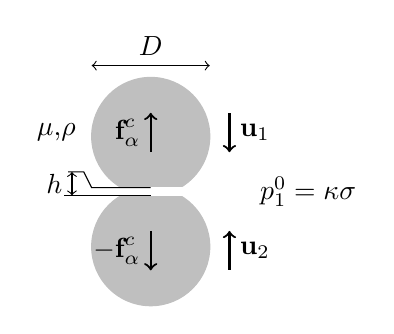
\begin{tikzpicture}
      \draw[lightgray,fill = lightgray] (0,0.7) circle (0.75);
      \draw[lightgray,fill = lightgray] (0,-0.7) circle (0.75);
      \draw[white,fill=white] (-0.75,-0.05) rectangle (0.75,0.05);
      \draw(0,0.05)--++(-0.75,0)--++(-0.1,0.2)--++(-0.2,0);
      \draw(0,-0.05)--++(-1.1,0);
      \draw[<->](-1,-0.05) --++ (0,0.3)node[midway,left]{$h$};
      \draw[<->](-0.75,1.6)--++(1.5,0)node[midway,above]{$D$};
      \node (para) at (-1.2,0.75){$\mu$,$\rho$};
      \node (pressure) at (2,0){$p_1^0 = \kappa \sigma$};
      \draw[->,thick](0,0.5)--++(0,0.5)node[midway,left]{$\textbf{f}_\alpha^\text{c}$};
      \draw[->,thick](0,-0.5)--++(0,-0.5)node[midway,left]{$-\textbf{f}_\alpha^\text{c}$};
      \draw[<-,thick](1,0.5)--++(0,0.5)node[midway,right]{$\textbf{u}_1$};
      \draw[<-,thick](1,-0.5)--++(0,-0.5)node[midway,right]{$\textbf{u}_2$};
    \end{tikzpicture}
    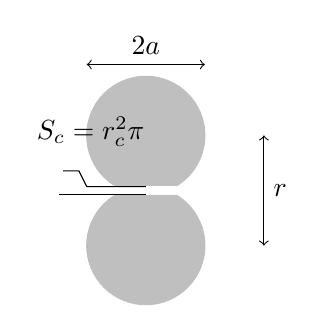
\begin{tikzpicture}
      \draw[lightgray,fill = lightgray] (0,0.7) circle (0.75);
      \draw[lightgray,fill = lightgray] (0,-0.7) circle (0.75);
      \draw[white,fill=white] (-0.75,-0.05) rectangle (0.75,0.05);
      \draw(0,0.05)--++(-0.75,0)--++(-0.1,0.2)--++(-0.2,0);
      \draw(0,-0.05)--++(-1.1,0);
      \draw[<->](-0.75,1.6)--++(1.5,0)node[midway,above]{$2 a$};
      \draw[<->](1.5,0.7)--++(0,-1.4)node[midway,right]{$r$};
      \node (para) at (-0.7,0.75){$S_c = r_c^2 \pi$};
    \end{tikzpicture}
    \caption{Scheme of two colliding droplets at close contact. Notice the null kurvature in the region of the interface close to the film leading to a capilary force $\textbf{f}_\alpha^\text{c} \approx - S_c \kappa \sigma \textbf{r}/|\textbf{r}|$. }
\end{figure}

Let use the following notation $(\bm{\sigma}_1' \cdot \textbf{n}_1)^\Sigma = \textbf{f}_\alpha = \textbf{f}_\alpha^\text{h}+\textbf{f}_\alpha^\text{c}$. 
It is clear, since the mean stress contribution $\div \bm{\sigma}_1$ isn't taken in account inside the drag force term, that the contribution $\textbf{f}_\alpha^\text{h}$ vanish or is negligible compared to $\textbf{f}_\alpha^\text{c}$ when the nearest particle is at a distance $|\textbf{r}| < a$ where $a$ is the.  Radius. 

If there is strong inhomogeneous structure in the flow the pure drag force term might be modified to yields the particle fluid particle stress. 
\begin{align*}
    n_p (\bm{\sigma}_1' \cdot \textbf{n}_1)_p^\Sigma
    &= 
    \int_{\mathrm{R}^3} (\bm{\sigma}_1' \cdot \textbf{n}_1)_\text{nst}^\Sigma
    P_\text{nst}(\textbf{x}\pm\textbf{r}/2,\mp\textbf{r}) d\textbf{r}
    +\div \int_{\mathrm{R}^3} \textbf{r} (\bm{\sigma}_1' \cdot \textbf{n}_1)_\text{nst}^\Sigma
    P_\text{nst}(\textbf{x},\textbf{r}) d\textbf{r}\\
\end{align*}
Which can be again decomposed into : 
\begin{align*}
    n_p (\bm{\sigma}_1' \cdot \textbf{n}_1)_p^\Sigma
    &= 
    \frac{1}{2}\int_{\mathrm{R}^3} \textbf{f}^h_\text{nst}P_\text{nst}(\textbf{x}\pm\textbf{r}/2,\mp\textbf{r}) d\textbf{r}
    + \frac{1}{2}\int_{\mathrm{R}^3} \textbf{f}^c_\text{nst}P_\text{nst}(\textbf{x}\pm\textbf{r}/2,\mp\textbf{r}) d\textbf{r} \\
    &
    +\div \int_{\mathrm{R}^3} \textbf{r} \textbf{f}_\text{nst}^\text{h} P_\text{nst}(\textbf{x},\textbf{r}) d\textbf{r}
    +\div \int_{\mathrm{R}^3} \textbf{r} \textbf{f}_\text{nst}^\text{c} P_\text{nst}(\textbf{x},\textbf{r}) d\textbf{r}\\
\end{align*}
The first term is the pure drag force components. 
The second terms is the pure contact force components which we will see to be null in the next section. 
Then, the third term is the particle-fluid-particle stress. 
And the last is the particle-film-particle stress. 


\subsubsection*{The contact forces}
In the same spirit as the classical surface force, as it is defined in \citet{jackson1997locally,zhang1997momentum,nott2011suspension} we can argue that the ensemble average of the close contact force cancel out. 
More precisely, the contact force on a single particle labeled $i$ due to the close contact with particle $j$ can be modeled by, 
\begin{equation*}
    \textbf{f}_{ij}^\text{c}
    = S_c \kappa \sigma \textbf{r}_{ij}/r_{ij}
    = \pi r_c^2 \kappa \sigma \textbf{r}_{ij}/r_{ij}
    = \pi (a^2 - r_{ij}^2/4) \kappa \sigma  \textbf{r}_{ij}/r_{ij}
\end{equation*} 
The resultants of these forces on the particle $i$ is therefore the sum of the contact with all particles except the $j^\text{th}$ particle, 
\begin{equation*}
    \textbf{f}_{i}^\text{c}
    = \sum_{j \neq i}\textbf{f}_{ij}
    = - \sum_{j \neq i} \pi (a^2 - r_{ij}^2/4) \kappa \sigma \textbf{r}_{ij}/r_{ij}
\end{equation*} 
The ensemble average of this force can be written using the classic point particle average,
\begin{align}    
\pavg{\textbf{f}_i^c}
&=
\int \sum_{i} \delta_i 
\textbf{f}_i^c d\PP 
= \int \sum_{i} \sum_{j \neq i} \delta(\textbf{x} - \textbf{x}_i) 
\textbf{f}_{ij}^c d\PP 
\\
\end{align}
Not that $\textbf{f}_{ij} = - \textbf{f}_{ji}$ however $\delta_i \textbf{f}_{ij} \neq - \delta_j\textbf{f}_{ji}$ thus the sum dosen't cancel drictly. 
Thus, following \citet{nott2011suspension,zhang1997momentum} we introduce the sum $\sum_j \delta(\textbf{x}-\textbf{x}_{ij}) \textbf{f}_{ij}^c =0$ where $\textbf{x}_{ij} = \textbf{x}_{ji} = (\textbf{x}_i+\textbf{x}_j)/2$.
Besides, notice that, 
\begin{equation*}
    \delta(\textbf{x} - \textbf{x}_{ij})
    = 
    \delta(\textbf{x} - \textbf{x}_i + ( \textbf{x}_{ij} - \textbf{x}_i))
    =
    \delta(\textbf{x} - \textbf{x}_i )
    - ( \textbf{x}_{ij} - \textbf{x}_i)\cdot \grad \delta(\textbf{x}-\textbf{x}_\alpha)
    +\frac{1}{2} (\textbf{x}_{ij} - \textbf{x}_i)(\textbf{x}_{ij} - \textbf{x}_i) : \grad\grad \delta(\textbf{x}-\textbf{x}_\alpha)
\end{equation*}
using both relation yields, 
\begin{align}    
    \pavg{\textbf{f}_i^c}
    &= \int \sum_{i} \sum_{j \neq i} [
        \delta(\textbf{x} - \textbf{x}_i)
        -\delta(\textbf{x} - \textbf{x}_{ij})]
    \textbf{f}_{ij}^c d\PP 
    \\
    &= \div \int \sum_{i} \sum_{j \neq i} \delta(\textbf{x}-\textbf{x}_i) (\textbf{x}_{ij} - \textbf{x}_i)
    \textbf{f}_{ij}^c d\PP 
    \\
    &= \frac{1}{2}\div \int \sum_{i} \sum_{j \neq i} \delta(\textbf{x}-\textbf{x}_i) (\textbf{x}_{j} - \textbf{x}_i)
    \textbf{f}_{ij}^c d\PP 
\end{align}
Using the formula for the contact force gives 
\begin{align}    
    \pavg{\textbf{f}_i^c}
    &= \frac{1}{2}\div \int \sum_{i} \sum_{j \neq i} \delta(\textbf{x}-\textbf{x}_i) 
    \textbf{r}\textbf{r}
    \pi (r^2/4 - a^2) /r \kappa \sigma d\PP 
    \\
\end{align}


\subsubsection*{Nearest stats for contacts forces in dilute case}
In the dilute case we consider only one conatc force so that, 
\begin{equation}
    n_p \textbf{f}^c_p = \iint 
    \sum_i 
    \delta(\textbf{x} -\textbf{x}_i)
    \sum_k 
    \textbf{f}_{k \to i}^\text{c} 
    \sum_{j\neq i}
    \delta(\textbf{x} + \textbf{r} -\textbf{x}_j) h_{ij}(t,\CC)
    d\PP d\textbf{r}\\
\end{equation}
Now we make use of a trick to cancel the pair particles forces by notticing that, 
\begin{equation}
    n_p \textbf{f}^c_p = \iint 
    \sum_k 
    \delta(\textbf{x} -\textbf{x}_k)
    \sum_i
    \textbf{f}_{i\to k}^\text{c} 
    \sum_{j\neq k}
    \delta(\textbf{x} + \textbf{r} -\textbf{x}_j) h_{kj}(t,\CC)
    d\PP d\textbf{r}\\
\end{equation}
So, we have, 
\begin{equation}
    n_p \textbf{f}^c_p = \frac{1}{2}\iint 
    \sum_i 
    \sum_k 
    \left[
        \sum_{j\neq i}
        \delta(\textbf{x} -\textbf{x}_i)
        \delta(\textbf{x} + \textbf{r} -\textbf{x}_j) h_{ij}
        \textbf{f}_{k \to i}^\text{c} 
        +
        \sum_{j\neq k}
        \delta(\textbf{x} -\textbf{x}_k)
        \delta(\textbf{x} + \textbf{r} -\textbf{x}_j) h_{kj}
        \textbf{f}_{i \to k}^\text{c} 
    \right]
    d\PP d\textbf{r}\\
\end{equation}
Note that the sums do not have the same restrictions. 
Nevertheless, this can be neglected since, if for example, $j=i$ we obtain $\delta(\textbf{x}-\textbf{x}_i)\delta(\textbf{x}+\textbf{r}-\textbf{x}_i) = 0$ thus the term cancel unless $\textbf{r}=0$ but let neglect that.
Besides, we must define manually that $h_{ii} = 0$ but it doesn't really matter.   
Or we get out these specifics case such as,
\begin{align}
    n_p \textbf{f}^c_p 
    &= \frac{1}{2}\iint 
    \sum_i 
    \sum_k 
    \sum_{j\neq k,i}
    \left[
        \delta(\textbf{x} -\textbf{x}_i)
        \delta(\textbf{x} + \textbf{r} -\textbf{x}_j) h_{ij}
        \textbf{f}_{k \to i}^\text{c} 
        +
        \delta(\textbf{x} -\textbf{x}_k)
        \delta(\textbf{x} + \textbf{r} -\textbf{x}_j) h_{kj}
        \textbf{f}_{i \to k}^\text{c} 
    \right]
    d\PP d\textbf{r}\\
    &+ \frac{1}{2}\iint 
    \sum_i 
    \sum_k 
    \left[
        \delta(\textbf{x} -\textbf{x}_i)
        \delta(\textbf{x} + \textbf{r} -\textbf{x}_k) h_{ik}
        \textbf{f}_{k \to i}^\text{c} 
        +
        \delta(\textbf{x} -\textbf{x}_k)
        \delta(\textbf{x} + \textbf{r} -\textbf{x}_i) h_{ki}
        \textbf{f}_{i \to k}^\text{c} 
    \right]
    d\PP d\textbf{r}\\
\end{align}

Now we must verify that this framework is coherent with the nearest particle statistics framework.
First we recall the definition of the pure drag term of the contact forces according to the neaerst particle statistics. 
\begin{align*}
    \pavg{\textbf{f}_i^\text{c}}
    &= \frac{1}{2}\int \nstavg{\textbf{f}_i^\text{c}} P_\text{nst}(\textbf{x}\pm\textbf{r}/2,\mp \textbf{r}) d\textbf{r}\\
    &=
    \frac{1}{2}\iint \sum_i \sum_{j\neq i}
    \delta(\textbf{x} \pm \textbf{r}/2 -\textbf{x}_i) 
    \delta(\textbf{x} \mp \textbf{r} -\textbf{x}_j) h_{ij}
    \textbf{f}_i^\text{c} 
    d\PP d\textbf{r}\\
    &=
    \frac{1}{2}\iint \sum_i \sum_{j\neq i}
    \delta(\textbf{x} \pm \textbf{r}/2 -\textbf{x}_i)
    \delta(\textbf{x} \mp \textbf{r} -\textbf{x}_j) h_{ij}
    \sum_{k} \textbf{f}_{ik}^\text{c} 
    d\PP d\textbf{r}\\
    &=
    \frac{1}{2}\iint \sum_i \sum_{j\neq i}
    \delta(\textbf{x} \pm \textbf{r}/2 -\textbf{x}_i)
    \delta(\textbf{x} \mp \textbf{r} -\textbf{x}_j) h_{ij}
     (\textbf{f}_{ij}^\text{c} + \sum_{k\neq i,j} \textbf{f}_{ik}^c)
    d\PP d\textbf{r}
\end{align*}
We must verify that both component of this integral cancel out. 
Changing teh integration sign we get,
\begin{equation*}
    \int \nstavg{\textbf{f}_i^\text{c}} P_\text{nst}(\textbf{x}, \textbf{r}) d\textbf{r}
    = \int \nstavg{\textbf{f}_i^\text{c}} P_\text{nst}(\textbf{x}, - \textbf{r}) d\textbf{r}
\end{equation*}
The drag force can alse, be written, 
\begin{equation*}
    \int [\textbf{f}^c_\text{eb}(\textbf{x}+\textbf{r}/2,\textbf{x} - \textbf{r}/2)+ \textbf{f}_\text{eb}^c(\textbf{x} -\textbf{r}/2,\textbf{x}+ \textbf{r}/2)]P_2(\textbf{x}\pm\textbf{r}/2,\textbf{x}\mp \textbf{r}/2) d\textbf{r}
    = \\
\end{equation*}
And since the contact force has only an antisymmetric contribution in average it is always true that in an averaged sense we have $\nstavg{\textbf{f}_i^\text{c}} P_\text{nst}(\textbf{x}, \textbf{r})  = - \nstavg{\textbf{f}_i^\text{c}} P_\text{nst}(\textbf{x}, - \textbf{r}) $, 
Additionally, 
\begin{align*}
    \pavg{\textbf{f}_\text{eb}^\text{c}}
    &=
    \frac{1}{2}\iint \sum_i \sum_{j\neq i}
    \delta(\textbf{x} + \textbf{r}/2 -\textbf{x}_i)
    \delta(\textbf{x} - \textbf{r}/2 -\textbf{x}_j) h_{ij}
    \sum_{k \neq i} \textbf{f}_{ik}^\text{c} 
    d\PP d\textbf{r}\\
    &=
    \frac{1}{2}\iint \sum_i \sum_{j\neq i}
    \delta(\textbf{x} + \textbf{r}/2 -\textbf{x}_i)
    \delta(\textbf{x} - \textbf{r}/2 -\textbf{x}_j) 
    h_{ij}
    \sum_{k \neq i} \textbf{f}_{ik}^\text{c} 
    d\PP d\textbf{r}\\
\end{align*}

\begin{align}    
\pavg{\textbf{f}_i^c}
&= \int_{|\textbf{r}|<a}
\int \sum_{i \neq j} \delta_i \sum_{j\neq i} \delta_j h_{ij}
\textbf{f}_i^c d\PP d\textbf{r}
= \int_{|\textbf{r}|<a}
\int \sum_{i \neq j} \delta_i \sum_{j\neq i} \delta_j h_{ij}
\sum_{k\neq i} \pi (r_{ik}^2/4 - a^2) \kappa \sigma \textbf{r}_{ik}/r_{ik} d\PP d\textbf{r}\\
&= \int_{|\textbf{r}|<a}
\int \sum_{i \neq j} \delta_i \sum_{j\neq i} \delta_j h_{ij}
\sum_{k\neq i} \pi (r_{ik}^2/4 - a^2) \kappa \sigma \textbf{r}_{ik}/r_{ik} d\PP d\textbf{r}
\\
\end{align}

Anyhow if we lake the assumption that this term indeed cancel we arrive at the expression: 
\begin{equation*}
    \int_{\mathrm{R}^3} \textbf{r} \textbf{f}_\text{nst}^\text{c} P_\text{nst}(\textbf{x},\textbf{r}) d\textbf{r}
    = 
\end{equation*}

\section{The dumping model}

Let decompose the drag force such that $\textbf{f}_\alpha = \textbf{f}_\alpha^h + \textbf{f}_\alpha^c$ with $^h$ being the hydrodynamical forces and $\textbf{f}^c_\alpha$ being the contatc forces. 
Let assume that the particle $\alpha$ interact with the particle $\beta$, where both particles has a radius $a$.
Let note $\textbf{r} = (\textbf{x}_\alpha - \textbf{x}_\beta) = \textbf{n} a$. 
Now let consider that the contact force can be modeled as a spring/dumping model with $k$ being the \textit{Raideur} and $c$ the dumping coefficient.
Then, the contact force between both particles can be written as, 
\begin{equation}
    \textbf{f}_\beta^c
    = \textbf{f}_{\alpha\beta}
    = (|\textbf{r}| - a) \textbf{n} k 
    + (\textbf{u}_\alpha - \textbf{u}_\beta) c
    \;\;\;\;\text{for} \;\;\; (|\textbf{r}| - a) < 0
\end{equation}
For smooth particle the second term can be reduced to the components along the normal vector \textbf{n}.  
Due to Newton's  law and since each interaction force cancel each other we have $\avg{\textbf{f}_\beta^c} \approx 0$. 
However, it is useful to notice that we have in the case of inhomogeneous scenario $\avg{\textbf{f}_\beta^c} \approx - \div \Sigma^c$.

Now let's focus on the source term of the granular temperature $\avg{\textbf{f}_\alpha\cdot \textbf{u}_\alpha'} = \avg{\textbf{f}_\alpha^h \cdot \textbf{u}_\alpha'} + \avg{\textbf{f}_\alpha^c\cdot \textbf{u}_\alpha'}$. 
The first source term $\avg{\textbf{f}_\alpha^h \cdot \textbf{u}_\alpha'} \sim k_p$ since $\textbf{f}_\alpha \sim \textbf{u}_\alpha$.

The part due to collision can be re written using the nearest averaged statistics formalism, 
\begin{align*}
    \avg{\textbf{f}_\alpha^c\cdot \textbf{u}_\alpha'}
    &= \int_{\textsc{R}^3}
    \int \sum_{\alpha \neq \beta} \delta_\alpha \delta_\beta h_{\alpha\beta}
    \textbf{u}'_\alpha \textbf{f}_\alpha^c d\PP d\textbf{r}\\
    &= \int_{\textsc{R}^3}
    \int \sum_{\alpha \neq \beta} \delta_\alpha \delta_\beta h_{\alpha\beta}
    \textbf{u}'_\alpha \cdot \textbf{n}
        (|\textbf{r}| - a) 
     d\PP d\textbf{r}
    + \int_{\textsc{R}^3}
    \int \sum_{\alpha \neq \beta} \delta_\alpha \delta_\beta h_{\alpha\beta}
    \textbf{u}'_\alpha 
         (\textbf{u}_\alpha - \textbf{u}_\beta) c
     d\PP d\textbf{r}\\
    &=k \int_{|\textbf{r}|<a}
    \nstavg{\textbf{u}'_\alpha \cdot \textbf{n}
        (|\textbf{r}| - a)   }
        P_{nst}(\textbf{x},\textbf{r})
     d\textbf{r}
    +c \int_{|\textbf{r}|<a}
        \nstavg{\textbf{u}'_\alpha 
         \cdot (\textbf{u}_\alpha - \textbf{u}_\beta)} P_\text{nst}(\textbf{x},\textbf{r})
     d\textbf{r}\\
\end{align*}
Elastic collisions are not dissipative therefore the first term cancel by definition. 
Thus, we are left with, 
\begin{align*}
    \avg{\textbf{f}_\alpha^c\cdot \textbf{u}_\alpha'}
    = c \int_{|\textbf{r}|<a}
        \nstavg{\textbf{u}'_\alpha 
         \cdot (\textbf{u}_\alpha - \textbf{u}_\beta)} P_\text{nst}(\textbf{x},\textbf{r})
     d\textbf{r} 
\end{align*}
\subsection{The dispersed phase equations}

Regarding the dispersed phase, we found the mass, momentum and total energy balance equations, 
\begin{align*}
    \pddt \left(n_p m_p\right)
    + \div \left(n_pm_p\textbf{u}_p
    \right)
    = 
    0\\
    \pddt \left(n_p m_p \textbf{u}_p\right)
    + \div \left(n_p
    m_p \textbf{u}_p \textbf{u}_p 
    - \bm{\sigma}_p^\text{eq}
    \right)
    = 
    n_p v_p  (  
    \rho_2 \textbf{g}
    - \grad p_1)
    + n_p (\bm{\sigma}_1'\cdot \textbf{n}_2)_p^\Sigma,\\
    \pddt(m_p n_pE_p^\text{tot})
    + \div(m_pn_p E_p^\text{tot} \textbf{u}_p 
    + \textbf{q}_p^\text{eq} - \textbf{u}_p \cdot \bm{\sigma}_p^\text{eq})
    =  n_p v_p [\rho_2 \textbf{u}_p\cdot  \textbf{g} 
    - \div (\textbf{u}_1 p_1)]\\
    +  n_p ( \textbf{u}'_1 \cdot \bm{\sigma}_1^0 \cdot \textbf{n}_2)_p^\Sigma
    -  n_p (\textbf{q}_1^0 \cdot \textbf{n}_2)_p^\Sigma
    +  n_p (\textbf{u}_1 \cdot \bm{\sigma}_1'\cdot \textbf{n}_2)_p^\Sigma
\end{align*}
where we have defined, 
\begin{align*}
    &\bm{\sigma}_p^\text{eq}
    = -  m_p\pnavg{\textbf{u}_\alpha'\textbf{u}_\alpha'}
    &\textbf{q}_p^\text{eq}
    =\textbf{q}_p^\text{e} 
    +\textbf{q}_p^\text{k}  
    +\textbf{q}_p^\text{w}  
    \\
    &\textbf{q}_1^\text{e}
    = m_p \pnavg{\textbf{u}_\alpha' e_\alpha'} 
    &\textbf{q}_p^\text{k}
    = m_p \pnavg{\textbf{u}_\alpha' k_\alpha} 
    \\
    &\textbf{q}_p^\text{w}
    = 
    + \pnavg{\textbf{u}_\alpha'(\rho_2 (w^0_2)^2/2 )'_\Omega}
    + \gamma \pnavg{\textbf{u}_\alpha' s_\alpha'}
\end{align*}

Now, subtracting each of these equations to the total NRJ equations yields, 


\tb{Think about doing a surface equation ? ? }
At the Lagrangian scale, 
\begin{equation*}
    \pavg{\ddt (m_\alpha E_\alpha + s_\alpha \gamma)}
    = 
     n_p (\rho_2 \textbf{u}_2^0  \cdot \textbf{g})^\Omega_p
    +n_p (\textbf{u}_1^0 \cdot \bm{\sigma}_1^0 \cdot  \textbf{n}_2)^\Sigma_p
    - n_p (\textbf{q}_1^0 \cdot \textbf{n}_2)^\Sigma_p
\end{equation*}
\begin{align}
    \pavg{\frac{1}{2}\ddt (m_\alpha u_\alpha^2)}
    &= 
    n_p (\rho_2 \textbf{u}_2^0 \cdot
    \textbf{g})_p^\Omega
    + 
    (\textbf{u}_\alpha\cdot
    \textbf{f}_\alpha)_p\\
    \pavg{\frac{1}{2}\ddt \left[\int_{\Omega_\alpha} \rho_2 (w_2^0)^2 d\Omega +s_\alpha \gamma\right] }
    &= (\textbf{w}_1^0 \cdot (\bm{\sigma}_1^0 \cdot \textbf{n}_2) )_p^\Sigma  
     - (\bm{\sigma}_2^0 : \grad\textbf{u}_2^0)_p^\Omega  
    \\
    \pavg{\ddt (m_\alpha e_\alpha )}
    &= 
     + n_p (\bm{\sigma}_2^0 : \grad\textbf{u}_2^0)^\Omega_p
    -  n_p (\textbf{q}_1^0 \cdot \textbf{n}_2 )_p^\Sigma
\end{align}
We first notice that, 
\begin{equation*}
    n_p\frac{1}{2}(m_\alpha u_\alpha^2)_p
    = n_p\frac{1}{2}m_p u_p^2
    +  k_p
\end{equation*}
Deriving the momentum kinetic NRJ equation for the particle phase and the above else we can have the following system of equations. 
\begin{align*}
    &\pddt \left(n_p m_p u_p^2/ 2\right)
    + \div \left(n_p
    m_p u_p^2/ 2 \textbf{u}_p 
    - \textbf{u}_p \cdot \bm{\sigma}_p^\text{eq}
    \right)
    = 
    - \bm{\sigma}_p^\text{eq}  :\grad \textbf{u}_p
    +  n_p v_p \textbf{u}_p \cdot (
    \rho_2 \textbf{g}
    - \grad p_1 )
    + n_p \textbf{u}_p \cdot (\bm{\sigma}'_1 \cdot \textbf{n}_2)^\Sigma_p,\\
    &\pddt \left(n_p (\rho_2 w^2 )_p^\Omega+\gamma s_p n_p\right)
    + \div 
    (n_p (\rho_2 w^2 )_p^\Omega+\gamma s_p n_p)
    \textbf{u}_p 
    +  \textbf{q}_p^\text{w}
    )
    = \\
    &- n_p (\bm{\sigma}_2^0 : \grad\textbf{u}_2^0)^\Omega_p
    + n_p (\textbf{u}_1 \cdot \bm{\sigma}_1' \cdot  \textbf{n}_2)^\Sigma_p
    + n_p (\textbf{u}_1' \cdot \bm{\sigma}_1^0 \cdot  \textbf{n}_2)^\Sigma_p
    -n_p v_p \grad (\textbf{u}_1p_1)
    - n_p (\textbf{u}_\alpha \cdot \bm{\sigma}_1^0 \cdot  \textbf{n}_2)^\Sigma_p
    \\
    &\pddt \left(n_p m_p e_p\right)
    + \div \left(n_p
    m_p e_p \textbf{u}_p 
    +  \textbf{q}_p^\text{e}
    \right)
    = 
    + n_p (\bm{\sigma}_2^0 : \grad\textbf{u}_2^0)^\Omega_p
    - n_p (\textbf{q}_1^0\cdot \textbf{n}_2)^\Sigma_p\\
\end{align*}

Now if we subtract these from the total NRJ equation one can show, 
\begin{multline*}
    \pddt(m_p n_pk_p)
    + \div(m_pn_p k_p \textbf{u}_p 
    + \textbf{q}_p^\text{k})
    = 
     \bm{\sigma}_p^\text{eq}  :\grad \textbf{u}_p
     + n_p v_p \textbf{u}_p \grad p_1
     + n_p (\textbf{u}_\alpha \cdot \bm{\sigma}_1^0 \cdot  \textbf{n}_2)^\Sigma_p
     - n_p \textbf{u}_p \cdot (\bm{\sigma}_1' \cdot  \textbf{n}_2)^\Sigma_p
    \\
\end{multline*}
Notice that, 















In order to be consistent with the fluid phase equations these terms must be written with $\textbf{f}_\text{pm} = n_p\textbf{u}_1 \cdot ((\bm{\sigma}_1^0 \cdot  \textbf{n}_2)^\Sigma_{nst}(\textbf{x} \pm \textbf{r}/2,\mp\textbf{r}) )_p$, and espetially  $\textbf{f}_\text{pm} = n_p ((\textbf{u}_1' \cdot\bm{\sigma}_1^0 \cdot  \textbf{n}_2)^\Sigma_{nst}(\textbf{x} \pm \textbf{r}/2,\pm\textbf{r}))_p$. Thus we need to reformulate. 
We use, 
\begin{align*}
    n_p (\bm{\sigma}_1^0 \cdot  \textbf{n}_2)^\Sigma_p
    = 
    n_p ( \bm{\sigma}_1' \cdot  \textbf{n}_2)^\Sigma_p
    - n_p (p_1   \textbf{n}_2)^\Sigma_p\\
    n_p (\textbf{u}_1^0 \cdot \bm{\sigma}_1^0 \cdot  \textbf{n}_2)^\Sigma_p
    = 
    n_p (\textbf{u}_1 \cdot \bm{\sigma}_1' \cdot  \textbf{n}_2)^\Sigma_p
    + n_p (\textbf{u}_1' \cdot \bm{\sigma}_1^0 \cdot  \textbf{n}_2)^\Sigma_p
    - n_p (\textbf{u}_1 p_1 \cdot  \textbf{n}_2)^\Sigma_p
\end{align*}
Notice that $\textbf{u}_1$ and $p_1$ varies slowly inside the volume of the particle.
Consequently we must use the relation, $\textbf{u}_1(\textbf{r}) = \textbf{u}_1(\textbf{x}_\alpha) + \textbf{r} \cdot\grad \textbf{u}_1(\textbf{x}_\alpha) \ldots$
and $p_1(\textbf{r}) = p_1(\textbf{x}_\alpha) + \textbf{r} \cdot\grad p_1(\textbf{x}_\alpha) \ldots$
to finnaly obtain, 
\begin{align*}
    n_p (\bm{\sigma}_1^0 \cdot  \textbf{n}_2)^\Sigma_p
    &= 
    n_p ( \bm{\sigma}_1' \cdot  \textbf{n}_2)^\Sigma_p
    - n_p v_p \grad p_1\\
    n_p (\textbf{u}_1^0 \cdot \bm{\sigma}_1^0 \cdot  \textbf{n}_2)^\Sigma_p
    &= 
    n_p (\textbf{u}_1 \cdot \bm{\sigma}_1' \cdot  \textbf{n}_2)^\Sigma_p
    + n_p (\textbf{u}_1' \cdot \bm{\sigma}_1^0 \cdot  \textbf{n}_2)^\Sigma_p
    - n_p v_p \div (\textbf{u}_1 p_1) \\
    &= 
    n_p \textbf{u}_1 \cdot( \bm{\sigma}_1' \cdot  \textbf{n}_2)^\Sigma_p
    + n_p (\textbf{r} \bm{\sigma}_1' \cdot  \textbf{n}_2)^\Sigma_p : \grad \textbf{u}_1
    + n_p (\textbf{u}_1' \cdot \bm{\sigma}_1^0 \cdot  \textbf{n}_2)^\Sigma_p
    - n_p v_p \div (\textbf{u}_1 p_1) \\
    &= 
    n_p \textbf{u}_1 \cdot \textbf{f}_{pm}
    + n_p (\mathcal{F}_p - \mathcal{F}_\text{pfp}): \grad \textbf{u}_1
    + n_p \textbf{c}_\text{pm}
    + \div [n_p(\mathcal{C}_\text{pfp} + \textbf{u}_1 \cdot \mathcal{F}_\text{pfp})]
    - n_p v_p \div (\textbf{u}_1 p_1) 
\end{align*}

\begin{align*}
    n_p (\textbf{w}_1^0 \cdot \bm{\sigma}_1^0 \cdot  \textbf{n}_2)^\Sigma_p
    &= 
    n_p (\textbf{u}_1^0 \cdot \bm{\sigma}_1^0 \cdot  \textbf{n}_2)^\Sigma_p
    - n_p (\textbf{u}_\alpha \cdot \bm{\sigma}_1^0 \cdot  \textbf{n}_2)^\Sigma_p\\
    n_p (\textbf{u}_\alpha \cdot \bm{\sigma}_1^0 \cdot  \textbf{n}_2)^\Sigma_p
    &=
    n_p (\textbf{u}_\alpha \cdot \bm{\sigma}_1' \cdot  \textbf{n}_2)^\Sigma_p
    - n_p (\textbf{u}_\alpha \cdot p_1 \cdot  \textbf{n}_2)^\Sigma_p
    % n_p (\textbf{u}_1 \cdot \bm{\sigma}_1' \cdot  \textbf{n}_2)^\Sigma_p
    % + n_p (\textbf{u}_1' \cdot \bm{\sigma}_1^0 \cdot  \textbf{n}_2)^\Sigma_p
    % - n_p v_p \div (\textbf{u}_1 p_1) \\
\end{align*}

In fact if we start back from the exact relation defined in the continuous pahse we can say that ,
\begin{align*}
    \avg{\delta_I (\bm{\sigma}_1^0 ) \textbf{n}_2} - p_1 \grad \phi_1
    = 
    % \avg{\delta_I (\bm{\sigma}_1^0 + p_1)\cdot \textbf{n}_2}
    % = 
    \avg{\delta_I \bm{\sigma}_1'\cdot \textbf{n}_2}
    \\
    \avg{\delta_I (\textbf{u}_1^0 \cdot\bm{\sigma}_1^0 )} - \textbf{u}_1p_1\cdot \grad \phi_1
    % = \avg{\delta_I (\textbf{u}_1 \cdot \bm{\sigma}_1' + \textbf{u}_1' \cdot \bm{\sigma}_1^0 )\cdot \textbf{n}_2}
    = \textbf{u}_1 \cdot \avg{\delta_I \bm{\sigma}_1'\cdot \textbf{n}_2}
    + \avg{\delta_I (\textbf{u}_1' \cdot \bm{\sigma}_1^0 )\cdot \textbf{n}_2}
\end{align*}

incoherence in teh exchange terms, 
\begin{align*}
    n_p (\textbf{u}_\alpha' \cdot \bm{\sigma}_1^0\cdot \textbf{n}_2)^\Sigma_p
    &= \int
    \sum_\alpha \delta_\alpha(\textbf{x} - \textbf{x}_\alpha)
    \textbf{u}_\alpha'(\CC,t)\cdot
    \left[\int_{\Sigma_\alpha} 
     (\bm{\sigma}_1^0 +p_1 \textbf{I})\cdot \textbf{n}_2
     d\textbf{r}
    - \int_{\Sigma_\alpha} 
     p_1  \textbf{n}_2
     d\textbf{r}\right]
     d\PP \\
    &= \int
    \sum_\alpha \delta_\alpha(\textbf{x} - \textbf{x}_\alpha)
    \textbf{u}_\alpha'(\CC,t)\cdot
    \left[\int_{\Sigma_\alpha} 
     \bm{\sigma}_1' +\cdot \textbf{n}_2
     d\textbf{r}
    - v_\alpha \grad p_1(\textbf{x}_\alpha)
    \right]
     d\PP \\
    &= n_p (\textbf{u}_\alpha' \cdot (\bm{\sigma}'_1\cdot \textbf{n}_2)^\Sigma )_p
    -  n_p (\textbf{u}_\alpha' v_p \cdot \grad p_1 )_p
     \\
    &= n_p (\textbf{u}_\alpha' \cdot (\bm{\sigma}'_1\cdot \textbf{n}_2)^\Sigma )_p
     \\
\end{align*}
Since $\textbf{u}_p$ is an Eulerian fields it must be evaluated at $\textbf{r}$ Therefore it must get out the 

Also, 
\begin{align*}
    n_p (\textbf{u}_1' \cdot \bm{\sigma}_1'\cdot \textbf{n}_2)^\Sigma_p
    &= \int
    \sum_\alpha \delta_\alpha(\textbf{x} - \textbf{x}_\alpha)
    \left[\int_{\Sigma_\alpha} 
    \textbf{u}_1'\cdot
    \bm{\sigma}_1^0\cdot \textbf{n}_2
    d\textbf{r}
    + \int_{\Sigma_\alpha} 
    \textbf{u}_1'\cdot
     p_1  \textbf{n}_2
     d\textbf{r}\right]
     d\PP \\
    &= n_p (\textbf{u}_1' \cdot \bm{\sigma}_1^0 \cdot \textbf{n}_2)^\Sigma_p
    -  n_p (\textbf{u}_1'[p_1  +  \textbf{r}\cdot \grad p_1 ]\cdot \textbf{n}_2 )_p^\Sigma
     \\
    &= n_p (\textbf{u}_1' \cdot \bm{\sigma}_1^0 \cdot \textbf{n}_2)^\Sigma_p
    -  n_p p_1  (\div \textbf{u}_1')_p^\Omega
    -  n_p (\textbf{u}_1'[p_1  +  \textbf{r}\cdot \grad p_1 ]\cdot \textbf{n}_2 )_p^\Sigma\\
    &= n_p (\textbf{u}_1' \cdot \bm{\sigma}_1^0 \cdot \textbf{n}_2)^\Sigma_p
    -  n_p\grad p_1\cdot ( \textbf{u}'_1)_p^\Omega
     \\
\end{align*}

Also, 
\begin{align*}
    n_p (\textbf{w}_2^0 \cdot \bm{\sigma}_1^0\cdot \textbf{n}_2)^\Sigma_p
    &= \int
    \sum_\alpha \delta_\alpha(\textbf{x} - \textbf{x}_\alpha)
    \cdot
    \left[\int_{\Sigma_\alpha} 
     \textbf{w}_2^0 (\bm{\sigma}_1^0 +p_1 \textbf{I})\cdot \textbf{n}_2
     d\textbf{r}
    - \int_{\Sigma_\alpha} 
     \textbf{w}_2^0 p_1  \textbf{n}_2
     d\textbf{r}\right]
     d\PP \\
    &= \int
    \sum_\alpha \delta_\alpha(\textbf{x} - \textbf{x}_\alpha)
    \left[\int_{\Sigma_\alpha} 
     \textbf{w}_2^0 \cdot \bm{\sigma}_1'\cdot \textbf{n}_2
     d\textbf{r}
    - \int_{\Sigma_\alpha} 
     \textbf{w}_2^0 (p_1 + \textbf{r}\grad p_1)   \textbf{n}_2
     d\textbf{r}\right]
     d\PP \\
     &= n_p (\textbf{w}_2^0 \cdot \bm{\sigma}_1' \cdot \textbf{n}_2)^\Sigma_p
    - n_p (p_1 \textbf{w}_2^0 \cdot \textbf{n}_2)^\Sigma_p\\
     &= n_p (\textbf{w}_2^0 \cdot \bm{\sigma}_1' \cdot \textbf{n}_2)^\Sigma_p
    - n_p (p_1 (\textbf{w}_2^0 \cdot \textbf{n}_2)^\Sigma)_p
    - n_p (\grad p_1\cdot ( \textbf{r} \textbf{w}_2^0 \cdot \textbf{n}_2)^\Sigma)_p\\
     &= n_p (\textbf{w}_2^0 \cdot \bm{\sigma}_1' \cdot \textbf{n}_2)^\Sigma_p
    - n_p (\grad p_1\cdot ( \div(\textbf{r} \textbf{w}_2^0))^\Omega)_p\\
     &= n_p (\textbf{w}_2^0 \cdot \bm{\sigma}_1' \cdot \textbf{n}_2)^\Sigma_p
    - n_p (\grad p_1\cdot ( \div\textbf{r} \textbf{w}_2^0)^\Omega)_p
    - n_p (\grad p_1\cdot ( \textbf{r} \div\textbf{w}_2^0)^\Omega)_p\\
     &= n_p (\textbf{w}_2^0 \cdot \bm{\sigma}_1' \cdot \textbf{n}_2)^\Sigma_p
\end{align*}







The averaged particle energy $n_p E_p$ can be split into five components,
\begin{equation*}
    n_p m_p E_p(t) 
    = m_p n_p e_p 
    + \pnavg{\int_{\Omega_\alpha(t)} \rho_2  (w_2^0)^2/2 d\Omega}
    + m_p n_p k_p
    + m_p n_p (u_p)^2/2
    + n_p s_p \gamma
    % + \textbf{u}_\alpha \cdot \int_{\Omega_\alpha(t)} \rho_2  \textbf{w}_2^0 d\Omega
\end{equation*}
where $k_p = \pavg{(u_\alpha')^2/2}$.
one equation for each is riquiered 
Using the mass balance and the momentum balance dotted with $\textbf{u}_p$ we obtain the particle kinetic energy balance, 
\begin{align*}
    \pddt \left(n_p m_p u_p^2/ 2\right)
    + \div \left(n_p
    m_p u_p^2/ 2 \textbf{u}_p 
    - \textbf{u}_p \cdot \bm{\sigma}_p^\text{eq}
    \right)
    = 
    - \bm{\sigma}_p^\text{eq}  :\grad \textbf{u}_p
    +  n_p v_p \textbf{u}_p \cdot (
    \rho_2 \textbf{g}
    - \grad p_1 )
    + n_p \textbf{u}_p \cdot \textbf{f}_{pm},\\
    \pddt \left(n_p (\rho_2 w^2 )_p^\Omega+\gamma s_p n_p\right)
    + \div 
    (n_p (\rho_2 w^2 )_p^\Omega+\gamma s_p n_p)
    \textbf{u}_p 
    +  \textbf{q}_p^\text{w}
    )
    = 
    - n_p \textbf{d}_p
    +  n_p (\textbf{u}_1 -\textbf{u}_p) \cdot  (\textbf{f}_{pm} - v_p \grad p_1)
    + n_p\textbf{c}_p\\
    \pddt \left(n_p m_p e_p\right)
    + \div \left(n_p
    m_p e_p \textbf{u}_p 
    +  \textbf{q}_p^\text{e}
    \right)
    = 
    + n_p \textbf{d}_p
    + n_p \textbf{e}_{pm},\\
\end{align*}
\tb{we remark that the collision tensor appear exactly at the same place as the pfp}
Subtracting all 3 equation to the total energy finally gives, 
\begin{align*}
    \pddt(m_p n_pk_p)
    + \div(m_pn_p k_p \textbf{u}_p 
    + \textbf{q}_p^\text{k})
    = 
    \bm{\sigma}_p^\text{eq} : \grad \textbf{u}_p
    % - n_p \textbf{d}_p
    - n_p v_p p_1 \div \textbf{u}_1
    + n_p (( \textbf{u}_\alpha' \cdot \bm{\sigma}_1^0 \cdot \textbf{n}_2)^\Sigma_\text{nst}(\textbf{x}\pm\textbf{r}/2,\mp\textbf{r}) )_p^r \\
\end{align*}
The transfer term of the internal droplets' fluctuation reads, 
\begin{align*}
    \int_{\Sigma_\alpha} \textbf{w}_1^0 \cdot (\bm{\sigma}_1^0 \cdot \textbf{n}_2) d\Sigma  
    = 
    (\textbf{u}_1 -\textbf{u}_\alpha) \cdot \int_{\Sigma_\alpha}  (\bm{\sigma}_1^0 \cdot \textbf{n}_2) d\Sigma  
    + \int_{\Sigma_\alpha} \textbf{u}_1' \cdot (\bm{\sigma}_1^0 \cdot \textbf{n}_2) d\Sigma  
    = (\textbf{u}_1 -\textbf{u}_\alpha) \cdot  (\textbf{f}_\alpha - \grad p_1)
    + \textbf{c}_\alpha
\end{align*}
\begin{align*}
    n_p (\textbf{w}_1^0 \cdot \bm{\sigma}_1^0 \cdot \textbf{n}_2)^\Sigma_p
    &= 
    n_p ((\textbf{w}_1^0 \cdot \bm{\sigma}_1^0 \cdot \textbf{n}_2)^\Sigma_\text{nst}(\textbf{x}\pm\textbf{r}/2,\mp\textbf{r}) )_p^r 
    + \div (n_p ( \textbf{r}(\textbf{w}_1^0 \cdot \bm{\sigma}_1^0 \cdot \textbf{n}_2)^\Sigma_\text{nst}(\textbf{x},\textbf{r}) )_p^r )\\
    &= 
    n_p (((\textbf{u}_1-\textbf{u}_\alpha) \cdot \bm{\sigma}_1^0 \cdot \textbf{n}_2)^\Sigma_\text{nst}(\textbf{x}\pm\textbf{r}/2,\mp\textbf{r}) )_p^r 
    +n_p ((\textbf{u}_1' \cdot \bm{\sigma}_1^0 \cdot \textbf{n}_2)^\Sigma_\text{nst}(\textbf{x}\pm\textbf{r}/2,\mp\textbf{r}) )_p^r \\
    &+ \div [n_p ( \textbf{r}((\textbf{u}_1 - \textbf{u}_\alpha) \cdot \bm{\sigma}_1^0 \cdot \textbf{n}_2)^\Sigma_\text{nst}(\textbf{x},\textbf{r}) )_p^r 
    + n_p ( \textbf{r}(\textbf{u}_1' \cdot \bm{\sigma}_1^0 \cdot \textbf{n}_2)^\Sigma_\text{nst}(\textbf{x},\textbf{r}) )_p^r ]\\
    &= 
    n_p (((\textbf{u}_1-\textbf{u}_\alpha) \cdot \bm{\sigma}_1^0 \cdot \textbf{n}_2)^\Sigma_\text{nst}(\textbf{x}\pm\textbf{r}/2,\mp\textbf{r}) )_p^r 
    +n_p \textbf{c}_{pm} \\
    &+ \div [n_p ( \textbf{r}((\textbf{u}_1 - \textbf{u}_\alpha) \cdot \bm{\sigma}_1^0 \cdot \textbf{n}_2)^\Sigma_\text{nst}(\textbf{x},\textbf{r}) )_p^r 
    + n_p \mathcal{C}_\text{pfp}]\\
\end{align*}
The remaining terms can be expressed as, 
\begin{align*}
    n_p (((\textbf{u}_1-\textbf{u}_\alpha) \cdot \bm{\sigma}_1^0 \cdot \textbf{n}_2)^\Sigma_\text{nst}(\textbf{x}\pm\textbf{r}/2,\mp\textbf{r}) )_p^r 
    &= 
    n_p (\textbf{u}_1 - \textbf{u}_p) \cdot (( \bm{\sigma}_1^0 \cdot \textbf{n}_2)^\Sigma_\text{nst}(\textbf{x}\pm\textbf{r}/2,\mp\textbf{r}) )_p^r \\
    &- n_p (( \textbf{u}_\alpha' \cdot \bm{\sigma}_1^0 \cdot \textbf{n}_2)^\Sigma_\text{nst}(\textbf{x}\pm\textbf{r}/2,\mp\textbf{r}) )_p^r \\
    &= 
    n_p (\textbf{u}_1 - \textbf{u}_p) \cdot(\textbf{f}_p - \grad p_1) \\
    &- n_p (( \textbf{u}_\alpha' \cdot \bm{\sigma}_1^0 \cdot \textbf{n}_2)^\Sigma_\text{nst}(\textbf{x}\pm\textbf{r}/2,\mp\textbf{r}) )_p^r \\
\end{align*}
The higher moments terms can be expressed as, 
\begin{align*}
    n_p (\textbf{r}((\textbf{u}_1-\textbf{u}_\alpha) \cdot \bm{\sigma}_1^0 \cdot \textbf{n}_2)^\Sigma_\text{nst})_p^r 
    &= 
    n_p (\textbf{u}_1 - \textbf{u}_p) \cdot (\textbf{r} ( \bm{\sigma}_1^0 \cdot \textbf{n}_2)^\Sigma_\text{nst} )_p^r 
    - n_p ( \textbf{r} ( \textbf{u}_\alpha' \cdot \bm{\sigma}_1^0 \cdot \textbf{n}_2)^\Sigma_\text{nst} )_p^r \\
    &= 
    n_p (\textbf{u}_1 - \textbf{u}_p)\cdot \mathcal{F}_\text{pfp} 
    - n_p (\textbf{r} ( \textbf{u}_\alpha' \cdot \bm{\sigma}_1^0 \cdot \textbf{n}_2)^\Sigma_\text{nst} )_p^r \\
\end{align*}
Alternatively, without the nearest particle formalism we obtain, 
\begin{align*}
    n_p (\textbf{w}_1^0 \cdot \bm{\sigma}_1^0 \cdot \textbf{n}_2)^\Sigma_p
    &= 
    n_p ((\textbf{w}_1^0 \cdot \bm{\sigma}_1^0 \cdot \textbf{n}_2)^\Sigma)_p 
\end{align*}

Averaging the microscopic 
\begin{align}
    \frac{1}{2}\ddt (m_\alpha u_\alpha^2)
    &= 
    \textbf{u}_\alpha\cdot
    \textbf{g}m_\alpha
    + 
    \textbf{u}_\alpha\cdot
    \textbf{f}_\alpha\\
    \frac{1}{2}\ddt \int_{\Omega_\alpha} \rho_2 (w_2^0)^2 d\Omega 
    + \ddt (s_\alpha \gamma) 
    &= 
    \int_{\Sigma_\alpha} \textbf{w}_1^0 \cdot (\bm{\sigma}_1^0 \cdot \textbf{n}_2) d\Sigma  
     - \int_{\Omega_\alpha} \bm{\sigma}_2^0 : \grad\textbf{u}_2^0 d\Omega  
    \\
    \ddt (m_\alpha e_\alpha )
    &= 
     \int_{\Omega_\alpha} \bm{\sigma}_2^0 : \grad\textbf{u}_2^0 d\Omega  
    -  s_\alpha \textbf{q}_\alpha  
\end{align}
Additionally, we can add an equation for the first moment of momentum, 
\begin{multline}
    \pddt \left(n_p \mathcal{P}_p\right)
    + \div \left(
        n_p \textbf{u}_p \mathcal{P}_p
    + \Sigma_p^\text{eq}
    \right)
    =
    n_p v_p \bm{\sigma}_1 
    + n_p \mathcal{F}_p\\
    +\pnavg{\int_{\Omega_\alpha} \left(
        \rho_2 \textbf{w}_2^0  \textbf{w}_2^0 
        - \bm{\sigma}_2^0
        \right) d\Omega}
        - \gamma  \pnavg{\int_{\Sigma_\alpha} \textbf{I}_{||} d\Sigma},
\end{multline}



\subsubsection{Modeling of collisions}

Even through we do not consider pure contact between interfaces it is still indispensable to define some kind of collision with the framework of the hybrid model. 
A contact mediated by the fluid is still different from near close contact, since in the latter case it is capillary pressure that drives the interaction forces. 

\subsection*{The drag force term}

The drag force term is easily closed by numerical method and some theoretical developments in the limiting case. 
Let now study the stokes 

\subsection*{Stress tensor for the continuous phase }
Regarding the fluid stress it can be reformulated considering Newtonian fluid,
\begin{equation}
    \phi_1 \bm{\sigma}_1 
    = - \phi_1 p_1 \textbf{I}
    + \mu_1 \phi_1 \textbf{e}_1
\end{equation}
with $\textbf{e}_1$ being the averaged shear rate. 
The first model is then, 
\begin{align*}
    \phi_1 \textbf{e}_1
    = \phi_1 (\nabla \textbf{u}_1+ (\grad \textbf{u}_1)^T)
    + \avg{[(\textbf{u}_1^0 - \textbf{u}_1)  \textbf{n}_1 +  \textbf{n}_1(\textbf{u}_1^0 - \textbf{u}_1 )]\delta_I}
\end{align*}
In \citet[chap 9]{ishii1975thermo} they assume,
\begin{equation}
    \avg{[(\textbf{u}_1^0 - \textbf{u}_1)  \textbf{n}_1 +  \textbf{n}_1(\textbf{u}_1^0 - \textbf{u}_1 )]\delta_I}\\
    = 
    (\textbf{u}_2 - \textbf{u}_1)  \grad \phi_1 +  \grad \phi_1(\textbf{u}_2 - \textbf{u}_1 )\\
\end{equation}
But I didn't find out where the derivation came from. 
Alternatively we can say that, 
\begin{align*}
    \phi_1 \textbf{e}_1
    = \nabla \textbf{u}+ (\grad \textbf{u})^T
    - \avg{\chi_2 (\grad\textbf{u}_2^0 + \grad(\textbf{u}_2^0 )^T)}
    = \textbf{e}
    - \phi_2 \textbf{e}_2
\end{align*}

More generally the stress within a suspension can be written,
\begin{align*}
    \bm{\sigma}_1 \phi_1
    &=- \phi_1 p_1 \textbf{I}
    + \mu_1 \textbf{e}
    - \lambda \phi_2 \bm{\tau}_2\\
    \bm{\sigma}_1 
    &= - \left(p_1 + \frac{\lambda \phi_2}{\phi_1} p_2\right) \textbf{I}
    + \frac{\mu_1}{\phi_1} \textbf{e}
    - \frac{\lambda \phi_2}{\phi_1} \bm{\sigma}_2\\
    \bm{\sigma}
    &= - \phi_1 p_1  \textbf{I}
    + \mu_1 \textbf{e}
    + \bm{\sigma}_2 \phi_2 
    +\phi_I \bm{\sigma}_I 
    - \lambda \phi_2 \bm{\tau}_2
\end{align*}
We can reformulate the last expression in the usual way using the first moment of momentum eq, 
\begin{equation}
    -  \dot{\mathcal{P}_p}
    +  \mathscr{S}_p^*
    +  \mathscr{L}_p
    + \frac{1}{3}(\bm{\sigma}_1^0 \cdot \textbf{n}_2 \cdot \textbf{r})_p^\Sigma \textbf{I}
    + n_p (\rho_2 \textbf{w}_2^0  \textbf{w}_2^0 )^\Omega
    =   (\bm{\sigma}_2^0)^\Omega
    + (\bm{\sigma}_I)^\Sigma,
\end{equation}
Or in stokes condition, 
\begin{equation}
    n_p \mathscr{S}_p^*
+ n_p \mathscr{L}_p
+ n_p\frac{1}{3}(\bm{\sigma}_1^0 \cdot \textbf{n}_2 \cdot \textbf{r})_p^\Sigma \textbf{I}
    = n_p \left(
        \bm{\sigma}_2^0
    \right)_p^\Omega
    +n_p (\bm{\sigma}_I)^\Sigma_p
\end{equation}
where we defined, 
\begin{align*}
    \mathscr{S}_p^* =\frac{1}{2} \pnavg{\int_{\Sigma_\alpha} \left(
        \textbf{r} \bm{\sigma}_1^0 \cdot \textbf{n}_2
        +  \bm{\sigma}_1^0 \cdot \textbf{n}_2\textbf{r}
        -
          \frac{2}{3}(\bm{\sigma}_1^0 \cdot \textbf{n}_2 \cdot \textbf{r})\textbf{I}
        \right)  d\Sigma}\\
    \mathscr{L}_p =\frac{1}{2} \pnavg{\int_{\Sigma_\alpha} \left(
        \textbf{r} \bm{\sigma}_1^0 \cdot \textbf{n}_2
        - \bm{\sigma}_1^0 \cdot \textbf{n}_2\textbf{r}
        \right) d\Sigma}
\end{align*}
Thus in homogeneous suspension without inertia we have, 
\begin{align*}
    \bm{\sigma}
    &= [- \phi_1 p_1 
    + n_p (\bm{\sigma}_1^0 \cdot \textbf{n}_2 \cdot \textbf{r})^\Sigma_p] \textbf{I}
    + \mu_1 \textbf{e}
    + n_p \mathscr{S}
    + n_p \mathscr{L}
\end{align*}
where the stress let is defined as $\mathscr{S} = \mathscr{S}_p^* - \lambda \phi_2 \bm{\tau}_2$. 
The equivalent stress in the fluid phase averaged equation can be reformulated as, 
\begin{align*}
    \bm{\sigma}_1^\text{eq}
    = \phi_1(
    \bm{\tau}_1%- n_p \textbf{M}_p
    - \rho_1 
    \kavg{\textbf{u}_1'\textbf{u}_1'})
    - n_p \mathcal{F}_\text{pfp} + n_p \mathcal{F}_p
    &= - (\phi_1 \rho_1  \kavg{\textbf{u}_1'\textbf{u}_1'}
        + n_p \mathcal{F}_\text{pfp})
        + \mu_1 \textbf{e} 
        - \lambda \phi_2 \bm{\tau}_2
         + n_p \mathcal{F}_p\\
    &= - (\phi_1 \rho_1  \kavg{\textbf{u}_1'\textbf{u}_1'}
        + n_p \mathcal{F}_\text{pfp})
        + \mu_1 \textbf{e} 
        - \lambda \phi_2 \bm{\tau}_2
         + n_p \mathscr{S}_p^*
         + n_p \mathscr{L}_p\\
    &= - (\phi_1 \rho_1  \kavg{\textbf{u}_1'\textbf{u}_1'}
        + n_p \mathcal{F}_\text{pfp})
        + \mu_1 \textbf{e} 
         + n_p \mathscr{S}_p
         + n_p \mathscr{L}_p
         + n_p (\bm{\sigma}_1^0 \cdot \textbf{n}_2 \cdot\textbf{r})_p^\Sigma \textbf{I}
\end{align*}
Thus, in the most general way the fluid phase stress can be written as that. 
But the last term must go into the equivalent pressure and that is a major founding. 
For netrally buoyant spherical particles : 
\begin{equation*}
    + n_p (\bm{\sigma}_1^0 \cdot \textbf{n}_2 \cdot\textbf{r})_p^\Sigma \textbf{I}
    = 
    n_p/a (p_1^0 )_p^\Sigma \textbf{I}
\end{equation*}
This, is definitely not trivial but if one wish to compute the first moment dynamical contribution to the suspension the formulas is given by 
\begin{align*}
    n_p \mathscr{S}_p
+ n_p \mathscr{L}_p
+ n_p\frac{1}{3}(\bm{\sigma}_1^0 \cdot \textbf{n}_2 \cdot \textbf{r})_p^\Sigma \textbf{I}
    &= 
    n_p \left(
        \bm{\sigma}_2^0
    \right)_p^\Omega
    +n_p (\bm{\sigma}_I)^\Sigma_p
    - \lambda \phi_2 \bm{\tau}_2\\
    &= 
    - n_p \left(
        p_2^0
    \right)_p^\Omega \textbf{I}
    +n_p (\bm{\sigma}_I)^\Sigma_p
    + n_p (1 - \lambda)\left(
        \mu_2 \textbf{e}_2^0
    \right)_p^\Omega 
\end{align*}
Let take the trace times $\frac{1}{3}$ of this equation, 
\begin{align*}
    \frac{1}{3} n_p(\bm{\sigma}_1^0 \cdot \textbf{n}_2 \cdot \textbf{r})_p^\Sigma 
    = 
    - n_p \left(
        p_2^0
    \right)_p^\Omega 
    +n_p \frac{1}{3}(\bm{\sigma}_I)^\Sigma_p : \textbf{I}
\end{align*}
Now let's substitute this equation into the former one, 
\begin{align*}
    n_p \mathscr{S}_p
+ n_p \mathscr{L}_p
=
    +n_p (\bm{\sigma}_I - \frac{1}{3}(\bm{\sigma}_I : \textbf{I})\text{I})^\Sigma_p
    + n_p (1 - \lambda)\left(
        \mu_2 \textbf{e}_2^0
    \right)_p^\Omega 
\end{align*}

If the particle is spherical, and that we remove the isotropic part on both sides of the equation we obtain 

In the spherical particle case the symmetric part reads, 
\begin{align*}
    n_p \mathscr{S}_p
    &= 
    + n_p (1 - \lambda)\left(
        \mu_2 \textbf{e}_2^0
    \right)_p^\Omega 
\end{align*}
which is false. 

\subsubsection{A translating sphere}
In the dilute stokes regime the disturbance velocity around a droplet can be written, 
\begin{align*}
    u_i^\text{Ext}(\textbf{r})
    = \left(\frac{\delta_{ik}}{r} + \frac{r_ir_k}{r^3}\right)  g_k
    + \left(-\frac{\delta_{ik}}{r^3} + \frac{3r_ir_k}{r^5}\right)  d_k\\
    u_i^\text{In}(\textbf{r})
    = c_i
    + \left(2 r^2 \delta_{ik} - r_ir_k\right) e_k\\
    e_{ik}
    = \mu(
        3 \delta_{ij} r_k 
        + 3 \delta_{kj} r_i
        -2 r_j \delta_{ki}
    )e_j 
\end{align*}
Applying the non deformation at the interface and other shear free condition we find the constant to be, 
\begin{align*}
    &\textbf{g} = \frac{1}{4}\left(\frac{3\lambda + 2}{\lambda +1}\right) a \textbf{U}
    &\textbf{d} = -\frac{1}{4}\left(\frac{\lambda}{\lambda +1}\right) a^3 \textbf{U}\\
    &\textbf{c} = \frac{1}{2}\left(\frac{3\lambda + 3}{\lambda +1}\right) \textbf{U}
    &\textbf{e} = -\frac{1}{2}\left(\frac{1}{\lambda +1}\right) \frac{1}{a^2} \textbf{U}\\
\end{align*}
Let consider isolated particles immersed in a viscous flow in the case $\textbf{u}_1' = \textbf{u}^{Ext}$.

The averaged internal shear rate $\phi_2 \textbf{e}_2$ can be thus estimated through the integral, 
\begin{align*}
    \avg{\chi_2 (\textbf{e}_2^0)_{ik}}
    &= \pavg{\int_{\Omega} \mu(
        3 \delta_{ij} r_k 
        + 3 \delta_{kj} r_i
        -2 r_j \delta_{ki}
    )e_j d\Omega}
    = 0\\
    &+ \div \pavg{\int_{\Omega} \textbf{r}\mu(
        3 \delta_{ij} r_k 
        + 3 \delta_{kj} r_i
        -2 r_j \delta_{ki}
    )e_j d\Omega}
\end{align*}
Also, the stress fields for such a flow is given by, 
\begin{equation*}
    T^G_{ijl} 
    = -6\frac{r_ir_jr_k}{r^5}
\end{equation*}

What about the first moment of momentum of the droplets, 
\begin{align*}
    (\mathcal{P}_p)_{ij}
    = \int_{\Omega} 
    u_i^\text{In} r_j 
    d\Omega
    = \int_{\Omega} 
    (c_i r_j 
    + 2 r^2  r_j e_i - r_i r_k r_j e_k)
    d\Omega
    = 0 
\end{align*}
Where we considered spherical particle with no deformation so it is obviously zero.
\begin{align*}
    (\textbf{w}_2^0 \textbf{w}_2^0)_{ij}^\Omega
    = \int_{\Omega} 
    u_i^\text{In}u_j^\text{In}
    d\Omega
    = \int_{\Omega} 
    ( c_i + \left(2 r^2 \delta_{ik} - r_ir_k\right) e_k)
    ( c_j + \left(2 r^2 \delta_{jl} - r_jr_l\right) e_l)
    d\Omega\\
    = \int_{\Omega} 
    (c_i c_j + c_i e_l (2 r^2 \delta_{jl} - r_jr_l )
    + (2 r^2 \delta_{ik} - r_ir_k)c_j e_k
    +  (2 r^2 \delta_{ik} - r_ir_k)(2 r^2 \delta_{jl} - r_jr_l)e_ke_l
    )
    d\Omega\\
    = c_i c_j v_\alpha
    + e_l c_i (2 \mathcal{M}_{kk} \delta_{jl} - \mathcal{M}_{jl})
    + e_k c_j (2 \mathcal{M}_{kk} \delta_{ik} - \mathcal{M}_{ik})\\
    + e_ke_l (\mathcal{M}_{kkkk}\delta_{ik}\delta_{jl}
    -2\mathcal{M}_{kkjl}\delta_{ik}
    -2\mathcal{M}_{kkik}\delta_{jl}
    + \mathcal{M}_{ikjl}) 
\end{align*}
\tb{problem on the units ; Re compute those Acknowledging that the inertia tensor is in fact completely isotropic}

The iternal energy, 
\begin{align*}
    (\textbf{w}_2^0 \textbf{w}_2^0)_{ii}^\Omega
    = \int_{\Omega} 
    u_i^\text{In}u_i^\text{In}
    d\Omega
    = \int_{\Omega} 
    ( c_i + \left(2 r^2 \delta_{ik} - r_ir_k\right) e_k)
    ( c_i + \left(2 r^2 \delta_{il} - r_ir_l\right) e_l)
    d\Omega\\
    = \int_{\Omega} 
    (c_i c_i + c_i e_l (2 r^2 \delta_{il} - r_ir_l )
    + (2 r^2 \delta_{ik} - r_ir_k)c_i e_k
    +  (2 r^2 \delta_{ik} - r_ir_k)(2 r^2 \delta_{il} - r_ir_l)e_ke_l
    )
    d\Omega\\
    = c_i c_i v_\alpha
    + e_l c_i (2 \mathcal{M}_{kk} \delta_{il} - \mathcal{M}_{il})
    + e_k c_i (2 \mathcal{M}_{kk} \delta_{ik} - \mathcal{M}_{ik})\\
    + e_ke_l (\mathcal{M}_{kkkk}\delta_{ik}\delta_{il}
    -2\mathcal{M}_{kkil}\delta_{ik}
    -2\mathcal{M}_{kkik}\delta_{il}
    + \mathcal{M}_{ikil}) 
\end{align*}
\subsubsection{A drop in shear flow}

The functional form of the internal velocity fields for a droplet immersed in a shear flow is,
\begin{align*}
    u_i^\text{Ext}(\textbf{r})
    = \left(\frac{\delta_{ij} r_l - \delta_{il} r_j - \delta_{jl} r_i}{r^3} 
    + \frac{r_ir_jr_l}{r^5}\right)  d_{jl}\\
    + \left(-3 \frac{\delta_{ij} r_l + \delta_{il} r_j + \delta_{jl} r_i}{r^5} 
    + 15\frac{r_ir_jr_l}{r^7}\right)  p_{jl}\\
    u_i^\text{In}(\textbf{r})
    = \left(- 4 \delta_{ij} r_l  + \delta_{il} r_j + \delta_{jl} r_i\right) f_{jl}\\
    e_{ik}
    = \mu [
        \partial_i \left(- 4 \delta_{kj} r_l  + \delta_{kl} r_j + \delta_{jl} r_k\right) f_{jl} + \partial_k \left(- 4 \delta_{ij} r_l  + \delta_{il} r_j + \delta_{jl} r_i\right) f_{jl} 
    ]\\
    = \mu [
        \left(- 4 \delta_{kj} \delta_{li}  + \delta_{kl} \delta_{ji} + \delta_{jl} \delta_{ki}\right) f_{jl} + \left(- 4 \delta_{ij} \delta_{lk}  + \delta_{il} \delta_{kj} + \delta_{jl} \delta_{ki}\right) f_{jl} 
    ]\\
    = \mu [
        \left(- 4 f_{ki}  + f_{ik} + f_{jj}\delta_{ki}\right)  + \left(- 4 f_{ik}  + f_{ki} + f_{jj} \delta_{ki}\right)  
    ]\\
    = \mu [
        \left(- 3 f_{ki}  - 3 f_{ik} +2 f_{jj}\delta_{ki}\right) 
    ]
\end{align*}
\todo[inline]{include the 3rd order terms to describe the internal flow}
Here i know that, 
\begin{align*}
    \textbf{d}
    = - \frac{1}{6} \left(
        \frac{2+5\lambda}{1+\lambda}a^3 \textbf{E}
    \right)
    &&
    \textbf{p}
    = - \frac{1}{6} \left(
        \frac{\lambda(2+5\lambda)}{(1+\lambda)(5\lambda+2)}a^3 \textbf{E}
    \right)
\end{align*}
Integrating this functional over the volume of a droplet yields, 
\begin{equation}
    \avg{\chi_2 (\textbf{e}_2^0)_{ik}}
    = \pavg{\int_{\Omega} 
        \mu [
        \left(- 3 f_{ki}  - 3 f_{ik} +2 f_{jj}\delta_{ki}\right) 
    ] d\Omega}
    = n_pv_p(-3 (f_{ki}+ f_{ik}) + 2 f_{jj} \delta_{ki})
\end{equation}
The only remaining thing is to do determine the form of $f_{ik}$. 


\subsection*{Continuous phase fluctuation term}

The Reynolds stress $\oneavg{\textbf{u}_1'\textbf{u}_1'}$ can be described in the limit of dilute non interaction particles by the wake. 
Therefore, by direct integration of $\textbf{u}^\text{Ext}$ we should be able to find a first correction of the velocity correlation. 
In a homogeneous flow of isolated particle ensemble average is equivalent to volume average thus, 
\begin{align*}
    \oneavg{\textbf{u}_1' \textbf{u}_1' }
    = \int u_i^\text{Ext} u_j^\text{Ext}(\textbf{x},\textbf{r}) P_1(\textbf{r}) d\textbf{r}\\
    = \int [\left(\frac{\delta_{ik}}{r} + \frac{r_ir_k}{r^3}\right)  g_k
    + \left(-\frac{\delta_{ik}}{r^3} + \frac{3r_ir_k}{r^5}\right)  d_k]
    [ \left(\frac{\delta_{jl}}{r} + \frac{r_jr_l}{r^3}\right)  g_l
    + \left(-\frac{\delta_{jl}}{r^3} + \frac{3r_jr_l}{r^5}\right)  d_l] d\textbf{r}
\end{align*}
The expansion of the fluctuation velocity is, i
\begin{align*}
    (\textbf{u}'_1)_i 
    (\textbf{u}'_1)_j
    &=
    \frac{g_i g_j}{r^{2}} 
    - \frac{d_i g_j}{r^{4}} 
    - \frac{d_j g_i}{r^{4}} 
    + \frac{g_i g_l x_j x_l}{r^{4}} 
    + \frac{g_j g_k x_i x_k}{r^{4}} \\
    &+ \frac{d_i d_j}{r^{6}} 
    - \frac{d_i g_l x_j x_l}{r^{6}} 
    - \frac{d_j g_k x_i x_k}{r^{6}} 
    + \frac{3 d_k g_j x_i x_k}{r^{6}} 
    + \frac{3 d_l g_i x_j x_l}{r^{6}} 
    + \frac{g_k g_l x_i x_j x_k x_l}{r^{6}} \\
    &- \frac{3 d_i d_l x_j x_l}{r^{8}} 
    - \frac{3 d_j d_k x_i x_k}{r^{8}} 
    + \frac{3 d_k g_l x_i x_j x_k x_l}{r^{8}} 
    + \frac{3 d_l g_k x_i x_j x_k x_l}{r^{8}} \\
    &+ \frac{9 d_k d_l x_i x_j x_k x_l}{r^{10}} 
\end{align*}
Since we kwon that this flow is axissymetri ctit can acctually be computed such thta
\begin{align*}
    (\textbf{u}'_1)_k 
    (\textbf{u}'_1)_l
    &= 
    ((\textbf{u}'_1)_i 
    (\textbf{u}'_1)_j p_j p_i) p_k p_l 
    + 
    ((\textbf{u}'_1)_i 
    (\textbf{u}'_1)_j (\delta_{ij} - p_j p_i))(\delta_{kl} -  p_k p_l )\\
    &= 
    ((\textbf{u}'_1)_i 
    (\textbf{u}'_1)_j )_{||} p_k p_l 
    + 
    ((\textbf{u}'_1)_i 
    (\textbf{u}'_1)_j )_{\bot}(\delta_{kl} -  p_k p_l )
\end{align*} 
where \textbf{p} is the normalized vector in the direction of \textbf{U}. 

Each of these terms must be integrated from $a$ to $\infty$ in a spherical coordinate frame. 
In spherical coordinate $d\textbf{r} = r^2 \sin\theta dr d\theta d\phi$. 
In this frame we have $x_0 = r \sin \theta \cos\phi$, $x_1 = r \sin \theta \sin\phi$ and $x_2 = r \cos\theta$.
Therefore, the first integration reads, 
\begin{equation*}
    \int_0^{2\pi} 
    \int_0^{\pi} 
    \int_1^{\infty} 
    \frac{1}{r^2} 
    r^2 \sin\theta dr d\theta d\phi
    = 
    4\pi 
    \int_1^\infty dr
\end{equation*}
This integral diverges thus it is not possibly feasible to compute such thing,
however we can relate the ensemble average to nearest conditional average by the relation : 
\begin{multline*}
    \avg{\chi_k \textbf{u}'_k\textbf{u}'_k}(\textbf{x},t)
    + \phi_k \textbf{u}_k\textbf{u}_k
    = \\
    \underbrace{\int (\nstavg{\chi_k \textbf{u}^0_k}  \nstavg{\chi_k \textbf{u}^0_k} / (\nstavg{\chi_k})  P_{nst}(\textbf{x},t,\textbf{r}) d\textbf{r} }_\text{PWFs}
    +\underbrace{\int \nstavg{\chi_k \textbf{v}_k^0\textbf{v}_k^0}  P_{nst}(\textbf{x},t,\textbf{r}) d\textbf{r}}_\text{WIA}
    \label{eq:def_uu}
\end{multline*}
where, $\textbf{v}_k^0  = \textbf{u}_k^0 - \nstavg{\chi_k \textbf{u}^0_k} / \nstavg{\chi_k}$ 
for a dillute random distribution, $P_\text{nst}^\text{th}(\textbf{y}|\textbf{x}) = n_p e^{-4 \pi n_p (r^3 - a^3)/3}$,

If we consider a flow in the $x$ direction we obtain for the three term sthe following integrands,
\begin{align*}
    \iint (\textbf{u}_1'\textbf{u}_1')_{00} r^2 \sin\theta d\phi d\theta
    = e^{\frac{4 \pi a^{3}}{3}}n_{p} \pi \frac{16}{5}\left(\frac{7   g^{2}_0  }{3} 
    + \frac{2   d_0 g_0 }{3 r^{2}} 
    + \frac{   d^{2}_0 }{ r^{4}} \right)e^{- \frac{4 \pi r^{3}}{3}}\\
    \iint (\textbf{u}_1'\textbf{u}_1')_{11}  r^2 \sin\theta d\phi d\theta
    =e^{\frac{4 \pi a^{3}}{3}}n_{p}\pi\frac{4}{5}
    \left(
        \frac{  g^{2}_0}{3} 
        + \frac{2   d_0 g_0 }{ r^{2}} 
        + \frac{3   d^{2}_0 }{ r^{4}}
    \right)e^{- \frac{4 \pi r^{3}}{3}}
\end{align*}
The remaining things to compute are the integral with respect to $\textbf{r}$ of the exponential function. 
Acknowledging that : 
\begin{align*}
    \int_a^\infty \frac{e^{- \frac{4 \pi r^{3}}{3}}}{r^4} dr
    = \frac{e^{- \frac{4 \pi a^{3}}{3}}}{3a^3}
    - \frac{4}{9} \pi \Gamma\left(0,\frac{4a^3\pi}{3}\right)
    = \frac{e^{- \frac{4 \pi a^{3}}{3}}}{3a^3}
    - \frac{4}{9} \pi E_1\left(\frac{4a^3\pi}{3}\right)
    \\
    \int_a^\infty \frac{e^{- \frac{4 \pi r^{3}}{3}}}{r^2} dr
    = \frac{E_{4/3}(\frac{4\pi a^3}{3})}{3a}\\
    \int_a^\infty e^{- \frac{4 \pi r^{3}}{3}} dr
    = \frac{a \Gamma\left(\frac{1}{3},\frac{4 a^2 \pi}{3}\right)}
    {6^{2/3} a \pi^{1/3}}
    = \frac{a E_{2/3}\left(-\frac{4 a^3 \pi}{3}\right)}
    {6^{2/3} a \pi^{1/3}}
\end{align*}
According to \texttt{Maxima} it gives, 
\begin{align*}
    \int_a^\infty \frac{e^{- \frac{4 \pi r^{3}}{3}}}{r^4} dr
    = 
    \frac{4\pi}{9} \Gamma\left(-1,\frac{4a^3\pi}{3}\right)
    \\
    \int_a^\infty \frac{e^{- \frac{4 \pi r^{3}}{3}}}{r^2} dr
    = {{2^{{{2}\over{3}}}\,\pi^{{{1}\over{3}}}\,\Gamma\left(-{{1
    }\over{3}} , {{4\,\pi\,a^3}\over{3}}\right)}\over{3^{{{4
    }\over{3}}}}}\\
    \int_a^\infty e^{- \frac{4 \pi r^{3}}{3}} dr
    = {{\Gamma\left({{1}\over{3}} , {{4\,\pi\,a^3}\over{3}}\right)}\over{
        3^{{{2}\over{3}}}\,4^{{{1}\over{3}}}\,\pi^{{{1}\over{3}}}}}
\end{align*}
The final results gives, 
\begin{align*}
    \iint (\textbf{u}_1'\textbf{u}_1')_{00} r^2 \sin\theta d\phi d\theta
    = e^{\frac{4 \pi a^{3}}{3}}n_{p} \pi \frac{16}{5}\left(\frac{7   g^{2}_0  }{3} 
    + \frac{2   d_0 g_0 }{3 r^{2}} 
    + \frac{   d^{2}_0 }{ r^{4}} \right)e^{- \frac{4 \pi r^{3}}{3}}\\
    \iint (\textbf{u}_1'\textbf{u}_1')_{11}  r^2 \sin\theta d\phi d\theta
    =e^{\frac{4 \pi a^{3}}{3}}n_{p}\pi\frac{4}{5}
    \left(
        \frac{  g^{2}_0}{3} 
        + \frac{2   d_0 g_0 }{ r^{2}} 
        + \frac{3   d^{2}_0 }{ r^{4}}
    \right)e^{- \frac{4 \pi r^{3}}{3}}
\end{align*}

\section*{Particle phase fluctuation}
In the same spirti as before we set, 
\begin{multline*}
    \avg{\delta_\alpha \textbf{u}'_\alpha\textbf{u}'_\alpha}(\textbf{x},t)
    + \phi_\alpha \textbf{u}_\alpha\textbf{u}_\alpha
    = \
    \underbrace{\int \nstavg{\delta_\alpha \textbf{u}_\alpha}  \nstavg{\delta_\alpha \textbf{u}_\alpha} / (\nstavg{\delta_\alpha})  P_{nst}(\textbf{x},t,\textbf{r}) d\textbf{r} }_\text{PWFs}
    +\underbrace{\int \nstavg{\delta_\alpha \textbf{v}_\alpha^0\textbf{v}_\alpha^0}  P_{nst}(\textbf{x},t,\textbf{r}) d\textbf{r}}_\text{WIA}
\end{multline*}
where, $\textbf{v}_\alpha = \textbf{u}_\alpha - \nstavg{\delta_\alpha \textbf{u}_\alpha}/\nstavg{\delta_\alpha}$. 

The aim is to predict $\nstavg{\delta_\alpha \textbf{u}_\alpha}$ knowing that the fluid velocity at $\textbf{r}$ is $\nstavg{\chi_1\textbf{u}^0_1}/\nstavg{\chi_1}$.

The velocity of the particle is found from teh momentum equation, 
\begin{equation*}
    \ddt \textbf{u}_\alpha
    = m_\alpha \textbf{g} + \textbf{f}_\alpha
\end{equation*}
In a statistical sens $\nstavg{\ddt \textbf{u}_\alpha}$ can be simplified. 
Then the force can be estimated as,
\begin{equation*}
    \nstavg{\textbf{f}_\alpha}
    = 6\mu \pi a 
    [\nstavg{\textbf{u}_\alpha} - \nstavg{\textbf{u}^0_1} + \nstavg{\grad^2 \textbf{u}_1^0}]
\end{equation*}
if teh particles are force free,
\begin{equation*}
    0
    = m_\alpha \textbf{g} 
    [\nstavg{\textbf{u}_\alpha} - \nstavg{\textbf{u}^0_1} + \nstavg{\grad^2 \textbf{u}_1^0}]
\end{equation*}
Therefore, 
\begin{equation*}
    \nstavg{\textbf{u}_\alpha} 
    =  \nstavg{\textbf{u}^0_1}
\end{equation*}

\subsection*{Computation of the Reynolds stress for potential flow }



\subsubsection{A note on the second moment of momentum equation}
It is said that : "Le second moment de la quantité de mouvement est une quantité nécessaire si on veut décrire les effets de la vitesse relative sur les contraintes"
Here it is :
\begin{multline}
    (r_{j}(\bm{\sigma}^0_2)_{ki}+r_{k}(\bm{\sigma}^0_2)_{ji})^\Omega
    +  (r_{j}(\bm{\sigma}^0_I)_{ki}+r_{k}(\bm{\sigma}_I^0)_{ji})^\Sigma
    = \\
    - \ddt (\rho_2 (\textbf{u}_2^0)_i r_j r_k)^\Omega
    + [\rho_2 (r_{j} (\textbf{w}_2^0)_k (\textbf{u}^0_2)_i + r_k (\textbf{w}_2^0)_j (\textbf{u}^0_2)_i)]^\Omega\\
    +(r_{k}r_{j} (\bm{\sigma}_1^0)_{il} (\textbf{n}_2)_l )^\Sigma
    + ( r_{k}r_{j}  \rho_2 d\Omega g_i)
\end{multline}
using the decomposition for the velocity $(\textbf{rwu}_2^0)^\Omega = (\textbf{rw}^0_2\textbf{w}_2^0)^\Omega + \textbf{u}_\alpha \mathcal{P}_\alpha $. Since only the symmetric part remain on the euaiton it reduce to $\textbf{u}_\alpha\mathcal{S}_\alpha$. 
The surface tension terms can be expressed,
\begin{equation}
    (r_{j}(\bm{\sigma}^0_I)_{ki})^\Sigma
    = (r_{j} (\delta_{ki} - n_kn_i)\gamma)
    = (r_{j}\delta_{ki}  - r_jn_kn_i)\gamma)^\Sigma
\end{equation} 
for spherical droplets this term vanish.
\begin{equation*}
    - \ddt (\rho_2 (\textbf{u}_2^0)_i r_j r_k)^\Omega
    = 
    - \ddt (\rho_2 (\textbf{w}_2^0)_i r_j r_k)^\Omega
    - \ddt ( u^\alpha_i \mathcal{M}_\alpha)
\end{equation*}
and the last term, 
\begin{equation*}
    ( r_{k}r_{j}  \rho_2 d\Omega g_i)
    = \textbf{g}_i \mathcal{M}^\alpha_{kj}
\end{equation*}














\subsection*{title} 


% %\section{Droplet deformation in stokestain dilute emulsions}
\section{Averaged equations for dispersed fluid-fluid flows with surface tension}%Newtonian dispersed two-phase flows with constant surface tension and no interfacial transfer}
\label{sec:averaged_surface}

%We now consider a dilute mono-disperse suspension of spherical droplet of radius $a$ without mass transfer. 
%The dispersed  and continuous phases are considered Newtonian fluids defined by the constant viscosities $\mu_k$ and density $\rho_k$.
%Additionally, the surface tension coefficient at the interface between both fluids is noted $\gamma$. 
%Because we consider a small droplet Reynolds number, we assert that only the averaged mass and momentum equations are sufficient to describe the mixture. 

We consider a monodisperse fluid-fluid suspension of droplets (or bubbles) which are not necessarily spherical with volume \( v_p \), in the absence of mass transfer. 
Both the dispersed and continuous phases are treated as incompressible Newtonian fluids, characterized by constant viscosities \( \mu_k \) and densities \( \rho_k \). 
The surface tension at the interface between the two fluids is denoted by \( \gamma \) which is not necessarily constant.%and is not a constant although we do not specify yet its .
%Although we do not specify the % and is  to be constant. 
%\JL{je ne pense pas que c'est necessaire de supposer que la tension de surface est constante ici}
We only consider in the next section averaged mass and momentum conservation equations to describe the motions of the phases. 
% \JL{tu dis cela car on ne consideres pas lenergie cinetique ?}
% In most of the industrial applications however, surfactants or/and non-uniform temperature gradient are present in the emulsion, both of which influence the value of the surface tension coefficient at the interface of the droplets.
% Hence, in this study we consider a non-uniform surface tension distribution at the interface of the droplets. 
\begin{table}
    \centering
    \begin{tabular}{|c|ccl|}\hline
    & Conservation law & mass & momentum \\ \hline
    Conserved quantity & $f_k^0$  & $\rho_k$ & $\rho_k \textbf{u}_k^0$ \\
    Source term & $s_k^0$  & $0$ & $\rho_k \textbf{g}$ \\
    Diffusive flux & $\Phi_k^0$ & 0 & $\bm\sigma_k^0 = -p_k^0 + \mu_k (\grad \textbf{u}_k^0 + \grad \textbf{u}_k^0)$ \\
    Surface diffusive flux & $\Phi_\Gamma^0$ & 0 & $\bm\sigma_\Gamma^0 = \gamma (\bm\delta - \textbf{nn})$ \\\hline
    \end{tabular}

    \caption{Definition of the physical quantities and local constitutive laws for phases $k$.}
    \label{tab:qte_Newtonian}
\end{table}
The conserved physical quantities  relevant to the problem are summarized in Table \ref{tab:qte_Newtonian}.


%\JL{quand apparait l'hypothese monodisperse ? -> je l'ai mise des le debut}

\JL{je ne suis pas trop fan du signe transposee que tu utilises qui est plutot useuellement utilise comme asterisque. d'ailleurs fait attention des fois il est place avant ou apres le terme en question. -> Brenner convention a specifier}

% \JL{j'ai l'impression qu'il y a des incoherences daans les parties au dessus: $\Phi _I -> \Phi _\Gamma$}

\JL{dans toute la section ci-dessous  $\textbf{n} -> \textbf{n}_d$ pour le terme de force ou alors definir n comme la normale a d des le debut.}


\JL{idem pour la notation $\phi_d$ est ce necessaire ?}



%The physical quantities to be conserved as well as the dimensionless number of the problem are summarized in \ref{tab:qte_Newtonian}. 
%After presenting in details the momentum equations for mono-disperse suspension of droplets, we dive into the closure problem. 
%In the averaged equation we neglect the droplet inertia, thus all the terms of $\mathcal{O}(Re \phi)$ are not considered.
%Moreover, we will consider spherical droplets, meaning that the terms of $\mathcal{O}(\phi Ca)$ are neglected as well.
%$Ca$ and $Re$ are the Capillary and Reynolds numbers defined \ref{tab:qte_Newtonian}, respectively. 
% In a second step we focus on how the droplet shape deviate from their spherical shape. 


%Following a detailed presentation of the momentum equations for a monodisperse suspension of droplets, we address the problem of the stress decomposition in the formulation of the moments.
%Then we address the closure problem of dilute monodisperse droplets in Stokes flow. 
%We recover the results obtained by \citet[Appendix B]{zhang1997momentum} and show how the higher order moments can be used to determine the droplets' shapes, and how they are connected to the continuous phase averaged equations. 
%We also discuss the form of the third-order force moments and some finite inertia closure.


After presenting the higher-order mass and momentum moments required to describe the particle rotation and deformation we derive the averaged equations for mass, momentum and first moment of momentum for a fluid-fluid suspension.
The presentation is inspired by \citep{lhuillier2009rheology}, while extending it beyond the scope of spherical solid particles.
Then we turn to the decomposition of stress within the moment formulation. 
The section concludes with a discussion of the symmetry properties of the effective stress tensor, employing arguments analogous to those presented by \citet{lhuillier1996contribution}.
%We finalize the section with a discussion on the symmetry of the effective stress tensor using arguments similar to \citep{lhuillier1996contribution}.

%In summary, we deal with the exact same scenario as 
%\citet[Appendix B]{zhang1997momentum}, i.e. dilute mono-disperse emulsion of inertialess droplets. 
%The goal of this section is not to demonstrate any new physical phenomenon, but rather to explain what is the meaning of the higher moment equations in this simple context, how they can be used to determine the droplets shapes, and how they are connected to the continuous phase averaged equations. 


\subsection{Higher-order mass and momentum moments}


\tb{peut etre mettre les equaitons fluid non-moyenne}

%Note that $\textbf{M}_\alpha$ is analogous to the inertia tensor $\textbf{I}_\alpha$ in solid mechanics, $\textbf{M}_\alpha$ and $\textbf{I}_\alpha$ are related through the expression $\textbf{I}_\alpha = (\bm\delta : \textbf{M}_\alpha)\bm\delta - \textbf{M}_\alpha$.
%For a fluid with a constant density, the tensor $\textbf{M}_\alpha$ describes the second moment of the volume distribution around the particle center of mass.
%Likewise, the tensor $\textbf{P}_\alpha$ describes the first moment of the velocity distribution within the particle volume. 
%To provide a clearer physical interpretation of the moment of momentum tensor, we decompose $\textbf{P}_\alpha$ into three distinct parts, denoted as $\textbf{S}_\alpha$, $\textbf{T}_\alpha$ and $P_\alpha$ such that,
%$\textbf{P}_\alpha = \textbf{S}_\alpha+\textbf{T}_\alpha + P_\alpha\bm\delta$, where $\textbf{S}_\alpha = \frac{1}{2}(\textbf{P}_\alpha + \textbf{P}_\alpha^\dagger - \frac{2}{3}(\bm\delta:\textbf{P}_\alpha)\bm\delta)$ represents the symmetric traceless part of $\textbf{S}_\alpha$ and $\textbf{T}_\alpha = \frac{1}{2}(\textbf{P}_\alpha - \textbf{P}_\alpha^\dagger)$ is the antisymmetric part of $\textbf{P}_\alpha$.
%Then, the tensors $\textbf{S}_\alpha$ and $\textbf{T}_\alpha$ correspond respectively to the stretching and angular momentum of the particle $\alpha$. 
%The tensor $\textbf{S}_\alpha$ quantifies how fast and in which direction the particle gets elongated or flattened, in other words it represents the mean rate of deformation experienced by the particle.
%The tensor $\textbf{T}_\alpha$ is related to the angular momentum of the particle denoted by the pseudo vector $\bm\mu_\alpha = \intO{ \rho_d \textbf{r} \times \textbf{u}_d^0 }$. 
%Indeed, both  $\textbf{T}_\alpha$ and $\bm{\mu}_\alpha$ represent the angular momentum and are related through $(\bm{\mu}_\alpha)_i = \epsilon_{ijk} (\textbf{T}_\alpha)_{jk} = \epsilon_{ijk} (\textbf{P}_\alpha)_{jk}$, where $\bm\epsilon$ is the third order alternating unit tensor or Levi-Cita tensor. 
%Lastly, we also introduce the scalar $P_\alpha =\frac{1}{3}\bm\delta : \textbf{P}_\alpha$, which quantifies the rate at which the particle is being compressed or expanded.
%In our case $P_\alpha =0$ because the interior velocity field of a droplet is assumed divergence free. 
%To better explain the implication of these quantities on the particle kinematics   we provide in \ref{eq:scheme}, three plots representing possible inner velocity fields with their corresponding value of the moment of momentum tensor.

To describe the dispersed phase in addition to the quantities defined in \ref{sec:Lagrangian} we define the second-order moment of mass and the first-order moment of momentum as 
\begin{equation}
    \textbf{M}_\alpha 
    = \intO{ \rho_d \textbf{r} \textbf{r} }
    \;\;\;\text{and}\;\;\;
    \textbf{P}_\alpha 
    = \intO{ \rho_d \textbf{r} \textbf{u}_d^0 },
    \label{eq:first_moment_of_momentum_def}
\end{equation}
respectively. 
Note that the tensor $\textbf{M}_\alpha$ plays a role analogous to the inertia tensor $\textbf{I}_\alpha$ in solid mechanics. 
The two are related by the expression  $\textbf{I}_\alpha = (\bm\delta : \textbf{M}_\alpha)\bm\delta - \textbf{M}_\alpha$.
For a fluid of constant density, $\textbf{M}_\alpha$ represents the second moment of the mass distribution relative to the particle center of mass.
Similarly, the tensor $\textbf{P}_\alpha$ is the first moment of the momentum distribution within the particle volume. 
To offer a clearer physical interpretation of the moment of momentum tensor, we decompose $\textbf{P}_\alpha$ into three distinct components  
\begin{equation}
\textbf{P}_\alpha = \textbf{S}_\alpha + \textbf{T}_\alpha + P_\alpha \bm\delta,
\end{equation}
where $\textbf{S}_\alpha = \frac{1}{2}\left(\textbf{P}_\alpha + \textbf{P}_\alpha^\dagger - \frac{2}{3}(\bm\delta:\textbf{P}_\alpha)\bm\delta\right)$ is the symmetric traceless part, representing the  deformation or stretching of momentum $\alpha$,
$\textbf{T}_\alpha = \frac{1}{2}(\textbf{P}_\alpha - \textbf{P}_\alpha^\dagger)$ is the antisymmetric part, associated with the angular momentum,
and $P_\alpha = \frac{1}{3} \bm\delta : \textbf{P}_\alpha$ is a scalar that quantifies the rate of isotropic expansion or compression. 
The angular momentum of the particle can also be expressed as the pseudo-vector  
$\bm\mu_\alpha = \int_\Omega \rho_d\, \textbf{r} \times \textbf{u}_d^0 \, dV$,
and is related to $\textbf{T}_\alpha$ via $(\bm\mu_\alpha)_i = \epsilon_{ijk} (\textbf{T}_\alpha)_{jk}$ %= \epsilon_{ijk} (\textbf{P}_\alpha)_{jk},
where $\epsilon_{ijk}$ is the Levi-Civita symbol.
Here, since the internal velocity field of a droplet is assumed to be divergence-free, we have $P_\alpha = 0$. 
To illustrate the physical significance of these tensors, we present in \ref{eq:scheme} three representative inner velocity fields, each with its corresponding moment of momentum tensor.
% Note that in \ref{eq:scheme} we explicit
\begin{figure}[h!]
    \centering
    \hfill
    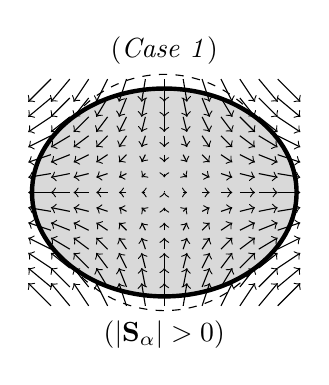
\begin{tikzpicture}[ultra thick,scale=0.6]
        \def\nRows{6}
        \def\nCols{6}
        \draw[dashed,thin] (0,0)circle(2.5);
        \draw[fill=gray!30] (0,0)ellipse(2.8 and 2.2);
        \foreach \x in {-\nRows,...,\nRows} {
            \foreach \y in {-\nCols,...,\nCols} {
                \pgfmathsetmacro\distance{veclen(\x*0.4, \y*0.4)};
                \pgfmathparse{\distance < 2.45 ? "blue" : "white"}
                \edef\colour{\pgfmathresult};
                \ifthenelse{\equal{\colour}{blue}}{                    
                    \draw[thin,->](\x*0.4,\y*0.4)--++(0.08*\x,-0.08*\y);
                }
            }
        }
        \node (txt) at (0,3){(\textit{Case 1})};
        \node (txt) at (0,-3){($|\textbf{S}_\alpha| > 0$)};
    \end{tikzpicture}
     \hfill
    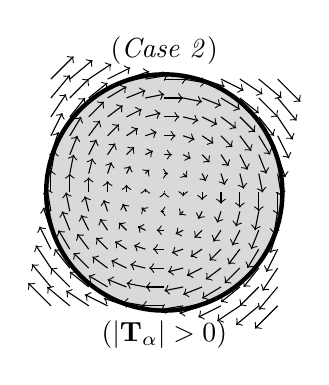
\begin{tikzpicture}[ultra thick,scale=0.6]
        \def\nRows{6}
        \def\nCols{6}
        \draw[fill=gray!30] (0,0)circle(2.5);
        \foreach \x in {-\nRows,...,\nRows} {
            \foreach \y in {-\nCols,...,\nCols} {
                \pgfmathsetmacro\distance{veclen(\x*0.4, \y*0.4)};
                \pgfmathparse{\distance < 2.5 ? "blue" : "white"}
                \edef\colour{\pgfmathresult};
                \ifthenelse{\equal{\colour}{blue}}{                    
                    \draw[thin,->](\x*0.4,\y*0.4)--++(0.08*\y,-0.08*\x);
                }
            }
        }
        \node (txt) at (0,3){(\textit{Case 2})};
        \node (txt) at (0,-3){($|\textbf{T}_\alpha| > 0$)};
    \end{tikzpicture}
    \hfill
    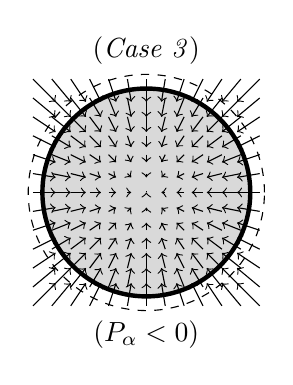
\begin{tikzpicture}[ultra thick,scale=0.6]
        \def\nRows{6}
        \def\nCols{6}
        \draw[dashed,thin] (0,0)circle(2.5);
        \draw[fill=gray!30] (0,0)circle(2.2);
        \foreach \x in {-\nRows,...,\nRows} {
            \foreach \y in {-\nCols,...,\nCols} {
                \pgfmathsetmacro\distance{veclen(\x*0.4, \y*0.4)};
                \pgfmathparse{\distance < 2.3 ? "blue" : "white"}
                \edef\colour{\pgfmathresult};
                \ifthenelse{\equal{\colour}{blue}}{                    
                    \draw[thin,->](\x*0.4,\y*0.4)--++(-0.08*\x,-0.08*\y);
                }
            }
        }
        \node (txt) at (0,3){(\textit{Case 3})};
        \node (txt) at (0,-3){($P_\alpha < 0$)};
    \end{tikzpicture}
    \hfill
    \caption{Graphical representation of the inner kinematics   of an arbitrary particle under three scenarios. 
        The arrows represent the velocity field inside the particle, $\textbf{w}_d^0$, with the corresponding value of the moment of momentum tensor indicated below. 
        The operator $|\ldots|$ refers to the norm of the tensors. 
        According to the inner velocity field:
        (\textit{Case 1}) The particle experiences a mean deformation, resulting in non-zero stretching of momentum along the principal axis of deformation;
        (\textit{Case 2}) The particle is rotating, leading to a non-zero angular momentum vector in the direction of rotation;
        (\textit{Case 3}) The particle undergoes compression, resulting in a negative trace of the moment of momentum.
    }
    \label{eq:scheme}
\end{figure}
Injecting, $f_d^0 = \rho_d$ in the second-order moment equation (derived in \ref{ap:Moments_equations}) we obtain,
%\JL{pq lequation du second moment de la masse ne fait pas intervenir la trace du premier moment de la qdm - cela semble incoherent ?}
\begin{equation}
    \ddt {\textbf{M}_\alpha}=2\textbf{S}_\alpha, %\JL{+2P_\alpha \bm\delta}, 
    \label{eq:dt_M_alpha}
\end{equation}
which is the second-order moment of mass conservation equation assuming that the fluid within the drop is divergence free. 
From \ref{eq:dt_M_alpha} we deduce that the evolution of the distribution of mass of a particle is solely determined by the stretching of momentum $\textbf{S}_\alpha$. 
This indicates that angular momentum does not influence the evolution of the second moment of mass, a consequence of the symmetry of the tensor $\textbf{M}_\alpha$, which must be preserved after differentiation with respect to time.
However, this does not imply that the particle angular velocity ($\bm\omega_\alpha$) does not appear in this equation. 
For instance, in the case of rigid body motion where $\textbf{w}_d^0 = \bm\omega_\alpha \times \textbf{r}$, we obtain the relation  $2\textbf{S}_\alpha = \bm\omega_\alpha \times \textbf{M}_\alpha+ \textbf{M}_\alpha\times \bm\omega_\alpha $. 
\JL{attention cette notation est bizarre : on fait un produit vectoriel entre un vecteur et un tenseur. l'ecrire sous forme indiciel ou faire reference a autre chose}
%Therefore, the angular velocity plays a significant role in the evolution of the second moment of mass equation. 

%\JL{ajouter lequation pour la derivee de $\textbf{S}_\alpha$ et discuter de celle pour la derivee seconde de $\textbf{M}_\alpha$}
Now that we have described the kinematics   of the particle shape, let us proceed to derive an equation for the moment of momentum.
This equation is derived by injecting $\textbf{Q}_\alpha^{(1)} = \textbf{P}_\alpha$ in \ref{eq:dt_Q_alpha_tot}, it reads, 
\begin{equation}
    \ddt {\textbf{P}_\alpha}
    - \intO{ \rho_d  \textbf{w}_d^0 \textbf{w}_d^0 }
    = 
    - \intO{\bm{\sigma}_d^0}
    - \intS{ 
        \gamma (\bm\delta - \textbf{nn})
    }
    + \intS{ \textbf{r}\bm{\sigma}_f^0\cdot \textbf{n}_d}.
    \label{eq:dt_P_alpha}
\end{equation}
The conservation equation of the angular momentum $\bm{\mu}_\alpha$ is obtained by taking the double contracted product of \ref{eq:dt_P_alpha} with $\bm\epsilon$, which directly gives
\begin{equation}
    \ddt\bm{\mu}_\alpha
    =  
    % \textbf{t}_\alpha.
    \intS{ \textbf{r} \times \bm{\sigma}_f^0\cdot \textbf{n}_d }
    \label{eq:dt_mu_alpha}
\end{equation}
Note that every term on the right-hand side of \ref{eq:dt_P_alpha} vanished due to their symmetric nature apart from the skew-symmetric part of the hydrodynamic stress, which is the hydrodynamic torque applied on the particle $\alpha$.
In particular, the surface tension terms do not appear in the angular momentum balance since the tensor $\bm\delta-\textbf{nn}$ is symmetric, which is consistent with the findings of \citet{hesla1993note}. 
As a consequence, the surface tension does not affect the angular momentum regardless of the particle shape. 
%In the literature, it is common to include the torque due to inter-particular interactions in the angular momentum balance, as is done in \citet{jackson1997locally} and \citet{zhang1997momentum}.
%In our case note that $\bm{\sigma}_f^0$ contains short-range hydrodynamic interaction forces. 

Taking the symmetric part of \ref{eq:dt_P_alpha}, and substrating the trace yields, 
\begin{align}
    &\ddt {\textbf{S}_\alpha}
    - \rho_d\intO{\left(\textbf{w}_d^0 \textbf{w}_d^0 -\frac{1}{3} (\textbf{w}_d^0 \cdot  \textbf{w}_d^0)\right)}
    = \nonumber \\
    &- 2\mu_d\intO{\textbf{e}_d^0}
    -  \intS{ \gamma
        \left( \frac{1}{3}\bm\delta - \textbf{nn} \right)
    }
    + \frac{1}{2}\intS{\left(\textbf{r}\bm\sigma_f^0+\bm\sigma_f^0\textbf{r}-\frac{2}{3}(\bm\sigma_f^0 \cdot \textbf{r})\bm\delta \right)\cdot \textbf{n}_d},
    \label{eq:dt_S_alpha}
\end{align}
%internal velocity kinetic energy. %$\intO{\rho_d\textbf{w}_d^0\textbf{w}_d^0 }$.
%On the left-hand side of \ref{eq:dt_S_alpha} we identify two inertial terms, i.e. the derivative of $\textbf{S}_\alpha$ and the stress induced by the product of internal velocity within the drop.
%The inertia of the particle is then balanced by the terms on the right-hand side of the equation, namely: 
%the volumic integral of the particle viscous stress; 
%the surface integral of the surface tension stress ; 
%and the first moment of the hydrodynamic stress tensor.
%A discussion regarding the physical implications of this equation is provided below. 
where we have introduced the rate of strain tensor for phase \( k \), defined as \( \mathbf{e}_k^0 = \frac{1}{2} (\nabla \mathbf{u}_k^0 + \nabla \mathbf{u}_k^0) \). 
On the left-hand side of Equation~\ref{eq:dt_S_alpha}, two inertial contributions can be identified: the time derivative of $\mathbf{S}_\alpha$, and the stress arising from the product of internal velocity field within the droplet. 
These inertial effects are counterbalanced by the terms appearing on the right-hand side of the equation, which include: the volume integral of the particle viscous stress; the surface tension moment; and the first moment of the hydrodynamic force.
%\JL{a finaliser}
While surface tension effects do not influence the linear or angular momentum equations directly, they do impact the moment of momentum $\textbf{P}_\alpha$, specifically its symmetric part $\textbf{S}_\alpha$.
Consequently, surface tension influences the hydrodynamic behavior of a particle exclusively through its effect on $\textbf{S}_\alpha$, which is related to the shape of a particle represented by $\textbf{M}_\alpha$, via \ref{eq:dt_M_alpha}.
%Whether it is solid or fluid particles \ref{eq:dt_S_alpha} becomes particularly relevant for expressing the averaged stress within an inertial suspension in terms of Lagrangian properties, as discussed in the next chapter. 
%\JL{enlever la trace}
%Taking the symmetric part of \ref{eq:dt_P_alpha}, and making use of \ref{eq:dt_M_alpha}, yields a dynamical balance equation for $\textbf{M}_\alpha$, namely
Inserting \ref{eq:dt_S_alpha} in  \ref{eq:dt_M_alpha} yields,
%\JL{enlever la trace et reecrire la partie ci-dessous + donner la definition de $e_d$ qui n'est pas de defini avant.}
\begin{align}    
    &\frac{1}{2}\frac{d^2 \textbf{M}_\alpha}{dt^2}
    =  \rho_d\intO{\left(\textbf{w}_d^0 \textbf{w}_d^0 -\frac{1}{3} (\textbf{w}_d^0 \cdot  \textbf{w}_d^0)\right)}
    - 2\mu_d\intO{\textbf{e}_d^0} \nonumber\\
    &- \intS{\gamma  
        \left( \frac{1}{3}\bm\delta - \textbf{nn} \right)
    }
    + \frac{1}{2}\intS{\left(\textbf{r}\bm\sigma_f^0+\bm\sigma_f^0\textbf{r}-\frac{2}{3}(\bm\sigma_f^0 \cdot \textbf{r})\bm\delta \right)\cdot \textbf{n}_d}.
    \label{eq:dt2_M_alpha}
\end{align}
%On the left-hand side of \ref{eq:dt_S_alpha}, we recover the symmetric part of the inertial contributions. 
%In opposition to \ref{eq:dt_P_alpha} we could substitute the term $\ddt (\textbf{P}_\alpha+\textbf{P}_\alpha^\dagger)$ initially present in the equation by $\ddt^2 \textbf{M}_\alpha$ using \ref{eq:dt_M_alpha}. 
%\ref{eq:dt2_M_alpha} is a second-order partial differential equation for the second order mass moment characterizing the droplet shape.
%In other words, \ref{eq:dt2_M_alpha} must be interpreted as an equation for the shape of the particle, represented by the tensor $\textbf{M}_\alpha$. 
%Thus, on the right-hand side of \ref{eq:dt_S_alpha}, we identify the terms which favors deformation, including the inertia of the velocity field within the droplet as well as the traceless part of the first moment and the terms wwohc resis deformation incluidng the viscous resistance within the droplet and the surface tension.
Equation \ref{eq:dt2_M_alpha} is a second-order differential equation governing the second-order mass moment that characterizes the droplet shape. 
In other words, it should be interpreted as an equation describing the droplet shape, represented by the tensor $\textbf{M}_\alpha$.
Accordingly, the right-hand side of \ref{eq:dt2_M_alpha} contains terms that promote deformation-such as the product of the internal velocity field and the traceless component of the first moment-as well as terms that oppose deformation, including droplet internal viscous resistance and surface tension.
%One might also recognize that \ref{eq:dt2_M_alpha} is in fact an extension of \citet{batchelor1970stress} result, but with the consideration of the inertia of the particle.
\ref{eq:dt2_M_alpha} is particularly useful to compute the unknown internal stress within solid particles, in terms of surface integral, i.e. the first moment of the hydrodynamic force.
This relation plays a key role in expressing the bulk stress of a suspension and ultimately leads to the effective viscosity, once a closed-form expression for the average first moment is obtained \citep{batchelor1970stress}. 
In the inertial regime, and for solid particles, the tensors $\textbf{M}_\alpha$ and the internal velocity field $\textbf{w}_d^0$ are fully prescribed by the particle kinematics. 
As a result, in equation \ref{eq:dt2_M_alpha}, $\textbf{M}_\alpha$ and $\textbf{w}_d^0$ appear not as unknowns but rather as known source terms.
For spherical particles specifically, the inertial correction to the first force moment has been derived by \citet{hwang1989modeling} and  \citet{lhuillier1996contribution}.
%For the specific case of spherical particles \citet{hwang1989,lhuillier1996contribution} have derived this inertial correction.
%This relation is used to express the bulk stress of a suspension.
%It eventually leads to the computation of the famous Einstein equivalent viscosity, upon having a closed expression for the average of the first moment \citep{guazzelli2011}. 
%In the inertial case and for solid particle, the tensors $\textbf{M}_\alpha$ and the inner velocity field $\textbf{w}_d^0$ are fully determined by the particle kinematic, indicating that $\textbf{M}_\alpha$ and $\textbf{w}_d^0$ can be used in \ref{eq:dt_S_alpha} not as unknowns but as source terms. 
%Consequently, for solid particles, \ref{eq:dt_S_alpha} must be interpreted as a generalized equation for the undefined stress $\bm\sigma_d^0$ integrated on the volume of the particles.

%Note that if intead we had considered spherical particles composed of compressible fluid \ref{eq:dt2_M_alpha} transforms into the Rayleigh-Lamb-Plesset equation as demonstrated in \citep{danielcours}.


%In our case, only the external contribution $\intS{\textbf{r}\bm\sigma_f^0\cdot \textbf{n}}$ is responsible for the generation of angular momentum, see \ref{eq:dt_mu_alpha}.
%Taking the symmetric part of this tensor ultimately removes this contribution. 

%\begin{equation}
%    \intO{\bm{\sigma}_d^0}
%    + \intS{\gamma(\bm\delta - \textbf{nn})}
%    = \frac{1}{2}\intS{(\textbf{r}\bm\sigma_f^0+\bm\sigma_f^0\textbf{r})\cdot \textbf{n}},
%    \label{eq:Batchelor}
%\end{equation}

%In \ref{ap:Moments_equations} we show how to derive the higher-order moment of momentum equations, which can also be viewed as formulas for the higher moments of the internal particle stress distribution. 
%It is interesting to mention that in a recent study of \citet{dolata2021faxen} and \citet{zhou2020lamb} they make use of the first two moments of momentum equations hidden into another but equivalent form, valid in the Stokes flow regime. 








\subsection{Averaged momentum and mass conservation equations}



Let us now focus on the averaged momentum equation of the continuous phase. 
By applying \eqref{eq:dt_f_k} with $f_k = \rho_f$ and $\rho_f\textbf{u}_f$ we obtain the mass and momentum equation for the continuous phase under the two fluid formulation, 
\begin{align}
    (\pddt + \textbf{u}_f\cdot \grad)\textbf{u}_f&=-\phi_f \div \textbf{u}_f
    \label{eq:mass_init}\\
    \phi_f \rho_f(\pddt + \textbf{u}_f  \cdot \grad) \textbf{u}_f
    % +  \div \avg{\chi_f\rho_f \textbf{u}_f'\textbf{u}_f'}
    &= 
    \div [\phi_f \bm\sigma_f-  \avg{\chi_f\rho_f \textbf{u}_f'\textbf{u}_f'}]
    + \phi_f \rho_f \textbf{g}
    - \avg{\delta_\Gamma \bm\sigma_f\cdot \textbf{n}}.
    \label{eq:two_fluid_momentum_init}
\end{align} 
To obtain the hybrid formulation one can expand the final term on the right-hand side of equation \ref{eq:two_fluid_momentum_init} using the Taylor expansion provided in \ref{eq:f_exp}.  
However, before doing so, it is important to examine the term \( \phi_f \bm\sigma_f \), as it contains a non-closed contribution originating from the averaging of the strain rate tensor. %a contribution from the dispersed phase. 
Properly identifying and isolating this contribution is a necessary step prior to performing the Taylor expansion.
%Moreover, there

%one may use \ref{eq:f_exp} to taylor expand the last term on the right-hand side of \ref{eq:two_fluid_momentum_init}. 
%However, it is first important to discuss the form of the term $\phi_f\bm\sigma_f$ since a dispersed phase term, is hidden into it, hence it is important to identify this term before carrying out the Taylor expansion. 

%\subsection{Mean stress formulation and momentum transfer decomposition}
%\JL{bien expliquer quand et comment apparaissent les distinctions sur le choix de la contrainte moyenne. en particulier voir en dessous}

We begin by noting that $\phi_f\bm\sigma_f$ can be expressed in terms of the averaged fluid pressure $p_f$, and continuous phase averaged velocity ($\textbf{u}_f$), or bulk-averaged velocity ($\textbf{u} = \phi_f \textbf{u}_f + \phi_d \textbf{u}_d$).
Expressing $\bm\sigma_f$ as a function of $\textbf{u}_f$ instead of $\textbf{u}$ (or vice versa) leads to two distinct forms of the momentum equation, each associated with different formulations of the closure terms. 
We also review several alternative choices found in the literature (see also \citet{jackson2000, pahtz2025general} for an overview focused on solid particles), emphasizing that while all these formulations are mathematically equivalent, they give rise to different closure problems. 
We argue that one particular formulation is probably the most suitable, especially in light of the closure terms available in the literature for non-dilute flows.%especially in the context of existing closure models for non-dilute flows.
%Choosing to express $\bm\sigma_f$ as a function $\textbf{u}_f$ rather than $\textbf{u}$ and vice versa, results in two distinct forms of the momentum equation and two distinct formulations of the closure terms. 
%We also discuss the various other choice available on the literature (see also \citet{jackson2000,pathz2025} for a review for solid particles) explaining that there is all choice are perfectly equivalent but leads to a different closure problems.
%Our belief his that there is one formulation which is the most appropriate with respect to of the closure terms available in the litterature for non-dilute flow.
%Although this topic has been already discussed in the context of solid particles  we propose here to expose both formulations and discuss which of the two equivalent (but different) formulations is the most suited for multiphase flow modeling. 

%Because we believe this topic has not been discussed much for non-solid particles in the literature, we propose here to expose both formulations and discuss which of the two equivalent (but different) formulation is the most suited for multiphase flow modeling. 
%Because we believe this topic has not been discussed much in the literature for non-solid particles, 

First we introduce what we refer to as the \textit{mean Newtonian stress}, based either on the continuous phase averaged velocity $\textbf{u}_f$ bulk velocity or on the \textbf{u}, namely,
\begin{align}
    \bm\Sigma_f 
    &
    = -p_f \bm\delta + 2\mu_f \textbf{E}_f    
    %= -p_f \bm\delta + \mu_f [\grad \textbf{u}_f + (\grad \textbf{u}_f)^{\dagger}], 
    \label{eq:Sigma_f_average}
    \\
    \bm\Sigma &
    = -p_f\bm\delta + 2 \mu_f \textbf{E}
    %= -p_f \bm\delta + \mu_f [\grad \textbf{u} + (\grad \textbf{u})^{\dagger}],
    \label{eq:Sigma_average}
\end{align}
where $\textbf{E}_f = [\grad \textbf{u}_f + (\grad \textbf{u}_f)^{\dagger}]/2$ and $\textbf{E} =[\grad \textbf{u} + (\grad \textbf{u})^{\dagger}]/2$ represent the \textit{mean strain rate} tensor based either on $\textbf{u}_f$ or on \textbf{u}. 
Additionally the ensemble averaged stress $\phi_f \bm\sigma_f$ may be written as 
\begin{equation}
    \phi_f \bm\sigma_f = - \phi _f p_f \bm\delta + 2 \mu_ f \phi_f \textbf{e}_f
    \label{eq:sigma_average}
\end{equation}
where $\phi _f \textbf{e}_f = \avg{\chi _f \textbf{e}_f^0}$. 
%Moreover by definition the bulk stress tensor reads $\textbf{E} = \phi _f\textbf{e}_f + \phi_d \textbf{e}_d$.
Inserting \ref{eq:Sigma_f_average} and \ref{eq:Sigma_average} in  \ref{eq:sigma_average} yields
%Using the constitutive law of Newtonian fluids we find, 
\begin{align}
    \phi_f \bm\sigma_f 
    &=
    % - \phi_f p_f \bm\delta
    % + \phi_f \mu_f [\grad \textbf{u}_f  + (\grad \textbf{u}_f)^\dagger]
    % - \mu_f \avg{\delta_\Gamma( \textbf{u}_f'  \textbf{n}_d +  \textbf{n}_d \textbf{u}_f' )}
    % =
    \phi_f \bm\Sigma_f
    - \mu_f \avg{\delta_\Gamma( \textbf{u}_f'  \textbf{n}_d +  \textbf{n}_d \textbf{u}_f' )}
    \label{eq:stress_closure}\\
    \phi_f \bm\sigma_f 
    &=
    % - \phi_f p_f \bm\delta
    % + \mu_f [\grad \textbf{u}  + (\grad \textbf{u})^\dagger]
    % - 2\mu_f \phi_d \textbf{e}_d
    % =
    \phi_f \bm\Sigma
    - \avg{2\mu_f \chi_d \textbf{e}_d^*}
    \label{eq:stress_closure1}
\end{align}
where we have used the relations 
\begin{equation}
    \avg{\chi_f \grad \textbf{u}_f^0}
    = 
    \phi_f \grad  \textbf{u}_f
    + \avg{\delta_\Gamma \textbf{n}_f \textbf{u}_f'}
    \label{eq:first_rel}
\end{equation}
and
\begin{equation}
    %\avg{\chi_f \textbf{e}_f^0}
%    = 
%    \avg{\textbf{e}^0}
%    - \avg{\chi_d \textbf{e}_d^0}
\phi _f\textbf{e}_f
%    = 
%    \textbf{E}
%    - \avg{\chi_d \textbf{e}_d^0}
    = 
    \phi_f \textbf{E}
    - \avg{\chi_d \textbf{e}_d^*},
    \label{eq:sec_rel}
\end{equation}
to derive \ref{eq:stress_closure,eq:stress_closure1}, respectively. 
 %in most practical situations of interest.
%Note that \ref{eq:first_rel} remains true in the presence of non zero interfacial rate of strain, while \ref{eq:sec_rel} requires the condition that the bulk rate of strain reads $\textbf{E} = \phi _f\textbf{e}_f + \phi_d \textbf{e}_d$ \textit{i.e.} that there is no shear stress at the interface of the droplets, so that $\avg{\delta_\Gamma \textbf{e}_\Gamma^0}= 0$, which is true in most of the practical cases of interest. 
In \ref{eq:stress_closure1} we have introduced $\textbf{e}_d^* = \textbf{e}_d^0 - \textbf{E} = \grad (\textbf{u}_d^0-\textbf{u})+\grad (\textbf{u}_d^0-\textbf{u})^\dagger$ which is the droplet internal shear rate relative to the `bulk' shear rate \textbf{E}.
%While $\textbf{u}_f' = \textbf{u}_f^0 - \textbf{u}_f$ in \ref{eq:stress_closure}. 
It is worth noting that equation \ref{eq:first_rel} remains valid even when the interfacial rate of strain is nonzero. 
In contrast, equation \ref{eq:sec_rel} holds under the assumption that the bulk rate of strain satisfies $\textbf{E} = \phi_f \textbf{e}_f + \phi_d \textbf{e}_d$, \textit{i.e.} that $\avg{\delta_\Gamma \textbf{e}_\Gamma^0} = 0$. 
This condition is supposed to be met here.
%Before presenting the hybrid form of the continuous phase momentum equation, it is interesting to expose the classic two-fluid formulation using the stress formulation given by \ref{eq:stress_closure} in the first place. 
%Before introducing the hybrid form of the continuous phase momentum equation, it is useful to first present the classical two-fluid formulation, employing the stress formulation \ref{eq:stress_closure}.
The averaged momentum equation  employing the stress formulation \ref{eq:stress_closure} read, 
\begin{align}
    % (\pddt + \textbf{u}_f\cdot \grad)\textbf{u}_f&=-\phi_f \div \textbf{u}_f\\
    \phi_f \rho_f(\pddt + \textbf{u}_f  \cdot \grad) \textbf{u}_f
    % +  \div \avg{\chi_f\rho_f \textbf{u}_f'\textbf{u}_f'}
    &= \phi_f 
    \left(\div \bm{\Sigma}_f
    + \rho_f \textbf{g}\right)
    - \div 
    [\avg{\chi_f\rho_f \textbf{u}_f'\textbf{u}_f'}
    +\avg{\delta_\Gamma \mu_f( \textbf{u}_f'  \textbf{n}_d +  \textbf{n}_d \textbf{u}_f')}]
    - \avg{\delta_\Gamma \bm\sigma_f^{(1)}\cdot \textbf{n}},
    \label{eq:two_fluid_momentum}
\end{align}
where, $\bm\sigma_f^{(1)}=\bm\sigma_f^0 - \bm\Sigma_f$ which also reads %is the Newtonian stress evaluated at a point on an interface relative to the mean stress $\bm\Sigma_f$. 
\begin{equation}
\bm\sigma_f^{(1)} = -p_f'\bm\delta
+ \mu_f [
    \grad \textbf{u}_f'
    + ^\dagger \grad \textbf{u}_f']
    \label{eq:disturbance_stress1}
\end{equation} 
Likewise, using \ref{eq:stress_closure1} one may also derive another form of the momentum equation, namely,
\begin{equation}
    \phi_f \rho_f(\pddt + \textbf{u}_f  \cdot \grad) \textbf{u}_f
    % +  \div \avg{\chi_f\rho_f \textbf{u}_f'\textbf{u}_f'}
    = \phi_f 
    \left(\div \bm{\Sigma}
    + \rho_f \textbf{g}\right)
    - \div 
    [\avg{\chi_f\rho_f \textbf{u}_f'\textbf{u}_f'} + \avg{2\mu_f \chi_d \textbf{e}_d^*}]
    - \avg{\delta_\Gamma \bm\sigma_f^{(2)}\cdot \textbf{n}},
    \label{eq:two_fluid_momentum2}
\end{equation} 
where $\bm\sigma_f^{(2)}=\bm\sigma_f^0 - \bm\Sigma$. 
%This stress tensor corresponds to the Newtonian stress (relative to the mean pressure and velocity field) typically available in numerical or theoretical studies. 
It can be also expressed as, 
%Clearly, subtracting by $\bm\Sigma_f$ to the local stress at the interface leads to the expression 
\begin{equation}
    \bm\sigma_f^{(2)} 
    =
    -p_f'\bm\delta
    + \mu_f [
        \grad \textbf{u}_f^*
        + ^\dagger \grad \textbf{u}_f^*
    ]
    \label{eq:disturbance_stress2}
\end{equation}
where $\textbf{u}_f^*= \textbf{u}_f^0 - \textbf{u}$.
%which corresponds to the Newtonian stress at the surface of the droplets (relative to the mean pressure and velocity field) typically available in numerical or theoretical studies.
%Likewise, substituting the mean stress with $\bm\Sigma$ in \ref{eq:disturbance_stress} one obtain the same formula except than $\textbf{u}_f'\to \textbf{u}_f^0 - \textbf{u}$. 
%Hence, 
In both cases (\ref{eq:two_fluid_momentum} and \ref{eq:two_fluid_momentum2}) one has to compute the local stress relative to the averaged continuous phase motion or bulk phase motion. 
% Note that because $\div \textbf{u} = 0$ it may be more convenient to  
%Note the differences between the last term of formulation \ref{eq:stress_closure} and \ref{eq:stress_closure1}, is equal to, $\phi_f (\div \bm\Sigma_f - \div\bm\Sigma)$
%Hence, the transition from one formulation to the other is straightforward, it just requires adding or subtracting $\phi_f (\div \bm\Sigma_f - \div\bm\Sigma)$. 
%However it is worth noting the physicsical meaning og this term which also reads,
Note the difference between the last terms in formulations \ref{eq:stress_closure} and \ref{eq:stress_closure1}, which is given by $\phi_f (\div \bm\Sigma_f - \div\bm\Sigma)$.
The transition from one formulation to the other is straightforward and only requires the addition or subtraction of this term. 
However, it is important to recognize its physical significance.
This difference can be expressed explicitly as,
\begin{equation}
    \phi_f (\div \bm\Sigma_f - \div\bm\Sigma) = \mu_f \phi_f \div \left(\grad (\phi _d \textbf{U}_r) + \grad (\phi _d \textbf{U}_r)^\dagger \right)
    \label{eq:diff_sigma1}
\end{equation}
%where $\textbf{u}_r = \textbf{u}_f - \textbf{u}_p$. 
%To derive this formula we make use of the relation $\textbf{u} = \phi_f \textbf{u}_f + \phi_d \textbf{u}_d$.
where $\textbf{U}_r = \textbf{u}_f - \textbf{u}_d$ is the phase averaged relative velocity between the fluid and dispersed phases, and the decomposition 
\begin{equation}
\textbf{u} = \phi_f \textbf{u}_f + \phi_d \textbf{u}_d,
\label{eq:u_mean} 
\end{equation}
has been used in the derivation.
Equation \ref{eq:diff_sigma1} reveals that the difference between the two formulations introduces a non-Newtonian stress term.
This non-Newtonian stress shares similarities with the second-order force moment closure \citep{jackson1997locally,zhang1997momentum}, and it typically related to intrinsic convection in sedimentation processes \citep{lhuillier2022}.
Therefore, when addressing the closure problem, it is essential to treat each stress formulation carefully, as the inclusion or exclusion of this additional term can significantly impact the resulting model.
%Then, when considering the colsure problem one has to be carefull to properly consider each formulation of the stress differently as both formulation will resulst in adding or removing this term.
%between \ref{eq:def_sigma_eff_f} and \ref{eq:def_sigma_eff_f2}  plus the differences between the corresponding drag force terms, is exactly equal to, $\phi_f (\div \bm\Sigma_f - \div\bm\Sigma)$.
%\JL{il faut que tu m'expliques : quand je soustrais les forces j'obtiens $\phi (\div \bm\Sigma_f - \div\bm\Sigma)$. OK on soustrait juste le RHS par ailleurs je pense qu'il faut detailler cela, c'est un point important.}
%\JL{en particulier $\div \bm\Sigma_f - \div\bm\Sigma = \div \nabla u_f - u \propto u_r$  a expliciter en montrant le developpment limite}





%Even though, both stress decomposition and momentum formulations proposed here are equivalent, each formulation have advantages and drawback which we discuss below.  
Although the stress decomposition and momentum formulations proposed herein are mathematically equivalent, each presents distinct advantages and limitations, which we examine in detail below.
%Now let us discuss on the choic between $\bm\Sigma$ and $\bm\Sigma_f$. 
%At first sight, using \ref{eq:dt_uf} with the effective stress given by \ref{eq:def_sigma_eff_f}, seems more practical because we are solving for the field $\textbf{u}_f$ hence avoiding the need of \ref{eq:velocity_conservation}. 
First, we may observe that a simplification arises for \ref{eq:stress_closure1} in the case of solid particles, for which $\textbf{e}_d^0 = 0$.
As a result $\phi _f \bm \sigma _f = - \phi _f p_f \bm\delta + 2 \mu_ f \textbf{E}$ \citep{joseph1990ensemble,jackson2000}. %and $\avg{\chi_d \textbf{e}_d^*} = -\phi_d\bm\Sigma$. \JL{a montrer}
Owing to this simplification, the formulation based on $\bm\Sigma$ and the associated closure relation \eqref{eq:stress_closure1} makes it a good candidate to be used in practice for solid particles. %is frequently adopted in the literature \citep{jackson2000}, despite requiring the inclusion of the additional momentum conservation equation.
Second, employing equation \ref{eq:two_fluid_momentum} with \ref{eq:disturbance_stress1} may appear more convenient as the governing equations are directly formulated in terms of the fluid velocity field $\textbf{u}_f$, thereby circumventing the need to explicitly include an expansion for the bulk fluid velocity. %the following equation
%Because $\textbf{u}$ may be required by \ref{eq:stress_closure1}, one also need to solve the equation, 
%\eqref{eq:velocity_conservation}.
%On the other hand we note that for solid particles $\textbf{e}_d^0 = 0$ and $\avg{\chi_d \textbf{e}_d'} = -\bm\Sigma\phi_d$, because of this great simplification \ref{eq:stress_closure1} is often used \citep{jackson2000} even if it requires adding \ref{eq:velocity_conservation} in the system of equation.  
%\JL{Je comprends l'interet de cette simplification, mais il faur toujours avoir une exression pr $\textbf{E}$ donc pour $\textbf{u}$}
Third, there exists a conceptual reason for preferring the bulk stress $\bm\Sigma$ when deriving closure relations for non-dilute suspensions.  %involving the fluctuating stress $\bm\sigma_f'$. 
Specifically, because $\bm\sigma_f^{(2)}$ depends on the disturbance velocity $\textbf{u}_f^* = \textbf{u}_f^0 - \textbf{u}$, the averaged velocity $\textbf{u}$ naturally serves as the "far-field" or "undisturbed" velocity boundary condition in the conditionally averaged Navier-Stokes equations \citep{hinch1977averaged,fintzi2025}. %(as also emphasized in the context of this PhD study).
%But there is another reason for using the `bulk stress' $\bm\Sigma$ as a reference stress to compute the closure terms involving $\bm\sigma_f'$. 
%Indeed, since $\bm\sigma_f'$ requires $\textbf{u}_f' = \textbf{u}_f^0 - \textbf{u}$, then \textbf{u} becomes the `far field' or `undisturbed' velocity boundary condition far from the test particle in the conditionally averaged Navier-Stokes equations \tb{(+my phd)}.
%On another hand, one may note that all the available theoretical solutions considering the disturbance field of a particle embedded in a pure solvent or in an effective medium (which represents other particles' contribution) use a divergence free `background flow' as limiting condition \citep{kim1985modelling,hinch1977averaged}.
%Since $\div \textbf{u} =0$ we deduce that the velocity field used in most (if not all) theoretical problems correspond to \textbf{u}. 
%Therefore, the disturbance  stress computed in these problems is $\bm\sigma_f'= \bm\sigma_f^0 - \bm\Sigma$. 
Notably, most (if not all) existing theoretical solutions addressing the disturbance field generated by a particle embedded in a Newtonian solvent or in an effective medium - representing other particles contribution - use a divergence-free background velocity field as limiting boundary condition \citep{hinch1977averaged, kim1985modelling}. 
Since $\nabla \cdot \textbf{u} = 0$, it follows that the velocity field used in these theoretical study corresponds to $\textbf{u}$. 
Consequently, the disturbance stress derived in those studies is $\bm\sigma_f^{(2)} = \bm\sigma_f^0 - \bm\Sigma$.
In opposition, the stress decomposition based on $\bm\Sigma_f$, involves the fields $\textbf{u}_f$ which is not divergence free. 
Hence, this `far field' or `undisturbed' velocity boundary condition far from the test particle does not correspond to the usual boundary condition assumed in most of the theoretical problems. 
%In conclusion, it is important to note that \textbf{u} corresponds exactly to the `background velocity' fields used in most of the theoretical derivations.
%Hence, the resulting closure terms (drag forces, stresslet and higher moments) derived in these studies refer to the closures expressed in terms of $\bm\sigma_f^0 - \bm\Sigma$.
%In all case one can always express $\bm\Sigma_f$ in terms of $\bm\Sigma$ hence which formulation to use is not a fatality. 
%However, one must always be careful when asserting that a given formulation of the drag force, for example, is exactly equivalent to a closure term found in the literature, as there are multiple possible formulations  (either based on $\bm\Sigma_f$, $\bm\Sigma$, $\bm\sigma_f$ or even  $p_f \bm\delta$). 
%Note that the choices between $\bm\Sigma_f$ and $\bm\Sigma$ only matter if one consider a closure problem, in which $\phi \textbf{u}_f \neq \phi \textbf{u}$, hence accurate at $\mathcal{O}(\phi^2)$ at least (such as in \citet{hinch1977averaged,kim1985modelling}). 
In conclusion, it is important to recognize that the vector field \(\textbf{u}\) corresponds precisely to the 'background velocity' typically employed in theoretical derivations. 
Consequently, the closure terms obtained in such analyses-such as drag forces, the stresslet, and higher-order moments-are formulated in terms of the difference \(\bm\sigma_f^0 - \bm\Sigma\).
However, it is always possible to express \(\bm\Sigma_f\) in terms of \(\bm\Sigma\) (see \ref{eq:diff_sigma1}), meaning that the choice of formulation remains free. 
Nevertheless, we must be cautious when claiming that a specific expression of, for example, the Faxen contribution to the force is exactly equivalent to a closure term reported in the literature especially for non-dilute suspension. 
%Multiple valid formulations exist, involving \(\bm\Sigma_f\), \(\bm\Sigma\), \(\bm\sigma_f\), or even the pressure tensor \(p_f \bm\delta\).
It should also be noted that the distinction between \(\bm\Sigma_f\) and \(\bm\Sigma\) becomes relevant only in the context of closure problems, particularly when \(\phi \textbf{u}_f \neq \phi \textbf{u}\), i.e., when effects at order \(\mathcal{O}(\phi^2)\) or higher are significant, as discussed in \citet{hinch1977averaged,kim1985modelling}.
\JL{pas compris cette derniere phrase que je pense il faut enlever : on montre que la distinction joue deja pour le second moment des forces en regime dilue non ?}

\JL{je n'ai pas compris le paragraphe suivant - je ne sais pas si il est necessaire desormais vu l'organisation actuelle ou on fait le developement en serie de Taylor plus tard}
% One can remark the similarities between the surface exchange terms expansion, and the multipole expansion used in microhydrodynamic that characterize the disturbance field caused by a body immersed in a stokes flow \citet{pozrikidis1992boundary,kim2013microhydrodynamics}. 
Moreover, one can wonder which of the formulation, \ref{eq:def_sigma_eff_f2} or \ref{eq:def_sigma_eff_f}, contains what is called the `Stresslet' and the higher moments of force given by the multipole expansion used in microhydrodynamic ? \citep{pozrikidis1992boundary,kim2013microhydrodynamics}\footnote{Note that the first term in this expansion is the same whether we use \ref{eq:def_sigma_eff_f2} or \ref{eq:def_sigma_eff_f}}.   
These moments are usually defined as the `extra stress above the value of the fluid law'\citep{hinch1977averaged}.
Because we are not studying the `bulk' momentum equation this definition does not directly apply in our context. 
However, note that \ref{eq:stress_closure1} involves the bulk velocity \textbf{u} which must be used in the bulk stress momentum equation.
Hence, we can state that the resulting formulation based on \ref{eq:stress_closure1} and given by \ref{eq:def_sigma_eff_f2}, corresponds to the multipole expansion of microhydrodynamic. 
\tb{not entirely sure but i think this is an important point }
Thus, the symmetric part of the second term of \ref{eq:def_sigma_eff_f2} is exactly what is called the `Stresslet', while the skew-symmetric part represents the hydrodynamic torque applied on the droplets.
The remaining terms of \ref{eq:def_sigma_eff_f2} represent the contribution of the second, third\ldots, and higher moments of hydrodynamic forces acted upon the droplets.  




%Additionally, because other stress decomposition have already been proposed in the literature we propose to discuss their advantages and draw back. 
%In the pioneering study of \citep{zhang1997momentum}, and in numerous articles that followed, the disturbance stress is defined as $\bm\sigma_f'= \bm\sigma_f^0 - \bm\sigma_f$ which is what we could call the ``intuitive'' definition. 
%However, note that using \ref{eq:stress_closure} one obtain that, 
Furthermore, given that various stress decomposition have already been introduced in the literature, we propose to examine their respective advantages and limitations. 
In the seminal work by \citet{zhang1997momentum}, as well as in numerous subsequent studies, the disturbance stress is defined as $\bm\sigma_f^{(3)} = \bm\sigma_f^0 - \bm\sigma_f$, a formulation that may be regarded as the "intuitive" definition. 
However, it is important to note that, by employing Equation~\ref{eq:stress_closure}, one obtains
\begin{equation}
    \bm\sigma_f^{(3)}
    = \bm \sigma _f ^{(1)}
%    -p_f'\bm\delta
%    + \mu_f [
%        \grad \textbf{u}_f'
%        + ^\dagger \grad \textbf{u}_f'
%    ]
    + \frac{\mu_f}{\phi_f} \avg{\delta_\Gamma( \textbf{u}_f'  \textbf{n}_d +  \textbf{n}_d \textbf{u}_f' )}
    \label{eq:stress_closure_zhang}
\end{equation}
%The first term on the rhight hand side of this expression correspond to the relative Newtonian stress usually integrated on the surface of a droplet or solid particle.
%The last term is a contribution related to the stress induced by the dispersed phase which normally appear in the effective stress expansion as shown below.
%To provide a better understanding of this term we assume that the suspension is made of solid particles $\textbf{e}_d = 0$.%for the following discussion 
The last term represents a contribution from the stress induced by the dispersed phase, as illustrated below. 
To better understand this term, we consider the case of a suspension composed of rigid solid particles, for which the strain rate tensor of the dispersed phase vanishes, i.e., $\textbf{e}_d = 0$.
%we remark that for solid particles . 
By subtracting \ref{eq:stress_closure} from \ref{eq:stress_closure1}, we directly obtain
\begin{equation}
    \avg{\delta_\Gamma (\textbf{n}_d \textbf{u}_f'+  \textbf{u}_f' \textbf{n}_d)}
    = 2 \mu _f \phi _f (\textbf{E}_f - \textbf{e} _f).
\end{equation} 
Since for solid particles $\textbf{e} _f = \textbf{E}/\phi _f$ we obtain,
\begin{equation}
    \avg{\delta_\Gamma (\textbf{n}_d \textbf{u}_f'+  \textbf{u}_f' \textbf{n}_d)} = 
    \textbf{U}_r\grad \phi_d + \grad \phi_d \textbf{U}_r   
%(\textbf{u}_f - \textbf{u}_d)\grad \phi_d + \grad \phi_d (\textbf{u}_f - \textbf{u}_d)
-  \phi_d [\grad \textbf{u}_d+ (\grad \textbf{u}_d)^\dagger ]. 
\label{eq:closure_un_nu}
\end{equation} 
where we have used \ref{eq:u_mean}.
Therefore, at least in the case of solid particles, this term becomes non-zero whenever there are significant gradients in volume fraction and mean particle velocity, as in the recent study by \citet{wang2024effect}.
%Therefore, at least for solid particles, this term is non-zero as soon as there are non-negligible gradients of volume fraction and mean gradients of particle velocities as in the recent work of \citet{wang2024effect}. 
%This finding implies that, in the recent work of \citet{wang2024effect}, where decomposition is employed for the drag force, we assert that they have actually computed the integral of the first two terms of \ref{eq:sigma_explict}, while neglecting the final term. 
%We conclude that the commonly used decomposition of the drag force introduced by \citet{zhang1997momentum,jackson2000}, given by \ref{eq:general_partition}, requires adding the term  $\avg{\delta_\Gamma (\textbf{n}_d \textbf{u}_f'+  \textbf{u}_f' \textbf{n}_d)}$ to the classical Newtonian stresses in the second term of \ref{eq:general_partition} and subtracting it in the mean drag force term (first term of \ref{eq:general_partition}). 
%Interestingly, \citet{wang2024effect}\footnote{
%    In this study the drag force is defined as the second term on the right-hand side of \ref{eq:drag_final} (see equation (3) of \citet{wang2024effect}).
%    They compute the drag force term using DNS by integrating $\bm\sigma_f^0$ over the particles surfaces, hence, assuming that $\bm\sigma_f=0$ (because there is no mean pressure gradient or velocity gradient).  
%    However, it is likely that the author overlooked the last term of \ref{eq:sigma_explict} which is non-zero \eqref{eq:closure_un_nu} in this specific scenario because $\grad \phi_d \neq 0$. 
%} specifically investigates the effect of the volume fraction gradient ($\grad \phi_d$) on the drag force. 
%\JL{a finaliser, rederiver la relation de Nico}
%Same comments apply if one consider \ref{eq:stress_closure1} in the above expression. 
%Hence, because $\bm\sigma_f$ already contains closure terms related to the dispersed phase, it appears to be prone to error to subtract the whole expression of $\bm\sigma_f$ from $\bm\sigma_f^0$.
The same observations hold if one considers expression \ref{eq:stress_closure1} in the analysis above. 
Since $\bm\sigma_f$ already includes closure contributions associated with the dispersed phase, directly subtracting the full expression of $\bm\sigma_f$ from $\bm\sigma_f^0$ can lead to inconsistencies unless the closure problem is handled with sufficient care.%if sufficient care is not done in the closure problem.
Nevertheless, note that because the last term of \ref{eq:stress_closure_zhang} is at most of $\mathcal{O}(\phi)$, the total contribution from this term when integrated on the droplets surface becomes of $\mathcal{O}(\phi^2)$, hence it can be safely neglected in dilute regime. 
\JL{pas compris cette derniere phrase.}

Another commonly adopted approach in the literature is $\bm \sigma ^{(4)} = \bm \sigma _f ^0 - p_f\bm\delta$ \citep{simonin1996,lhuillier2009rheology,morel2015mathematical,guazzelli2018rheology}.
This definition leads to the expression
\begin{equation}
    \bm\sigma_f^{(4)}  = -p_f' \bm\delta + \mu_f (\grad \textbf{u}_f^0 + ^\dagger \grad \textbf{u}_f^0),
\end{equation}
which implies that the closure is based on the absolute local fluid velocity $\textbf{u}_f^0$, rather than the fluctuating component $\textbf{u}_f'$.
%Hence the closure are computed based on the absolute local velocity $\textbf{u}_f^0$ instead of $\textbf{u}_f'.
%or in the case with buoyant particles simply $\sigma ^{(4)} = \bm \sigma _f ^0 - \rho_f\bm\delta$ \citep{lhuillier}
%One may also consider using  instead of $\bm\sigma_f$, $\bm\Sigma_f$ or $\bm\Sigma$, as done in \citet{morel2015mathematical} (\tb{paper de daniel ou il fait ca ?}), in this case $\bm\sigma_f'  = -p_f' \bm\delta + \mu_f (\grad \textbf{u}_f^0 + ^\dagger \grad \textbf{u}_f^0)$, hence the closure are computed based on the absolute local velocity $\textbf{u}_f^0$ instead of $\textbf{u}_f'$.
Without going into the details, note that numerous closures are based on the reciprocal theorem formulation \citep{kim2013microhydrodynamics,stone2001inertial,raja2010inertial}.%, this includes the Faxen contribution to the drag force . %the expressions given by the famous Faxen laws.
The closures (drag forces, stresslet etc... ) provided by the reciprocal theorem are by construction expressed in terms of the disturbance fields ($p_f'$,$\textbf{u}_f'$), because they must decay to zero far from the test particle. 
%Therefore, this last formulation may not be the most practical as well\footnote{
For example, the Faxen contribution to the drag force in the case of a spherical solid particle of radius $a$ is given by $\textbf{f} = \pi a^3 \mu_f \grad^2 \textbf{u}_f$. 
This formulation is obtained  by considering the contribution from the disturbance stress, $\bm\sigma ^{(1)}  = -p_f' \bm\delta + \mu_f (\grad \textbf{u}_f' + ^\dagger \grad \textbf{u}_f')$, which vanish far from the test particle. 
If one uses the formulation based on $\bm\sigma_f^{(4)}  = -p_f' \bm\delta + \mu_f (\grad \textbf{u}_f^0 + ^\dagger \grad \textbf{u}_f^0)$, the Faxen contribution to the drag force becomes $\textbf{f} = \pi a^3 \mu_f \grad^2 \textbf{u}_f + \frac{4\pi a^3}{3}\mu_f \grad^2 \textbf{u}_f$ where the second term is the contribution from the mean velocity field.
Although both formulations are equally valid, the second one appears to be less commonly used and could potentially lead to misinterpretations or inconsistencies if not carefully handled. 
%}. 


\JL{ajouter a la discussion le choix de Jackson et Pahtz si tu le souhaites mais moi j'ai la flemme}

%Because of those remarks, we will use in the following the formulation based on $\bm \sigma^{(2)}$ i.e. \ref{eq:two_fluid_momentum2} since we believe this is a formulation less prone to errors when considering the closure problem. 
%Moreover this is the formulation used in the closure problem for non-dilute flows. 
%For simplicity we will denote $\bm \sigma^{(2)} = \bm \sigma ^{*}$ in the rest of the paper.
%since we are working at $\mathcal{O}(\phi)$.
In light of these considerations, we adopt the formulation based on $\bm \sigma^{(2)}$-i.e., Equation \ref{eq:two_fluid_momentum2}-for the remainder of this work, as it is less prone to errors when considering the closure problem. 
Furthermore, this formulation is commonly employed in the analysis of non-dilute flows. 
For simplicity, we will denote $\bm \sigma^{(2)}$ as $\bm \sigma^{*}$ throughout the rest of the paper.
%This will avoid the need for \ref{eq:velocity_conservation} in the system of equation. 
%\tb{on pourrait utiliser aussi lautre peut importe }
%\JL{finaliser la discussion sur le fait que $\Sigma$ est le moins prine to errors + more ealsily extendeable to non dilute fraction}
%The last two terms on the right-hand side of \ref{eq:two_fluid_momentum} can be further expanded into a Taylor series using \ref{eq:f_exp_delta}. 
%Doing so leads us to the hybrid formulation of the continuous phase momentum  equation %(i.e. \ref{eq:avg_hybrid_dt_chi_f} %with $f_f^0 = \textbf{u}_f^0\rho_f$), namely,
%This gives the hybrid formulation of the continuous phase momentum equation,
%\begin{align}
%    \phi_f \rho_f(\pddt + \textbf{u}_f  \cdot \grad) \textbf{u}_f
%    &= \phi_f 
%    \left(\div \bm{\Sigma}_f
%    + \rho_f \textbf{g}\right)
%    + \div \bm\sigma_f^{(1)\text{eff}}
%    - \pSavg{\bm\sigma_f^{(1)}\cdot \textbf{n}}, 
%    \label{eq:dt_uf}
%\end{align}
%where we introduced the effective stress, 
%\begin{align}
%    \bm{\sigma}^{(1)\text{eff}}_f 
%    &= 
%    - \avg{\chi_f\rho_f \textbf{u}_f'\textbf{u}_f'} 
%    + \pSavg{[\textbf{r}\bm\sigma^{(1)}_f\cdot \textbf{n} - \mu_f (\textbf{u}_f' \textbf{n} + \textbf{n} \textbf{u}_f')]}\nonumber\\
%    &- \div
%        \pSavg{[\frac{1}{2}\textbf{rr}\bm\sigma^{(1)}_f\cdot \textbf{n}- \mu_f\textbf{r} (\textbf{u}_f' \textbf{n} + \textbf{n} \textbf{u}_f')]}
%        + \grad\grad (\ldots)
%    \label{eq:def_sigma_eff_f}
%\end{align}
%\JL{a finaliser}
The last two terms on the right-hand side of \ref{eq:two_fluid_momentum2} can be further expanded into a Taylor series using \ref{eq:f_exp_delta}.
Doing so leads us to the hybrid formulation of the continuous phase momentum  equation, %a relation similar to \ref{eq:dt_uf} except that $\bm\Sigma_f$ is replaced by $\bm\Sigma$, $\pSavg{\bm\sigma_f^{(1)}\cdot \textbf{n}}$ by $\pSavg{\bm\sigma_f^{(2)}\cdot \textbf{n}}$ and the effective stress $\bm\sigma_f^\text{(1)eff}$ by the tensor
\begin{align}
    \phi_f \rho_f(\pddt + \textbf{u}_f  \cdot \grad) \textbf{u}_f
    &= \phi_f 
    \left(\div \bm{\Sigma}
    + \rho_f \textbf{g}\right)
    + \div \bm\sigma_f^{\text{eff}}
    - \pSavg{\bm\sigma_f^{*}\cdot \textbf{n}}, 
    \label{eq:dt_uf2}
\end{align}
where,
\begin{align}
    \bm{\sigma}^{\text{eff}} 
    &= 
    - \avg{\chi_f\rho_f \textbf{u}_f'\textbf{u}_f'} 
    + \pavg{\intO{\textbf{r}\bm\sigma^{*}_f\cdot \textbf{n}} - \delta_p\intO{2\mu_f\textbf{e}_d^*}}\nonumber\\
    &- \div
        \pavg{ \frac{1}{2}\intS{\textbf{rr}\bm\sigma^{*}_f\cdot \textbf{n}}
        - \delta_p\intO{2\mu_f \textbf{r} \textbf{e}_d^*}}
        + \grad\grad (\ldots). 
    \label{eq:def_sigma_eff_f2}
\end{align}
Under these forms, the left-hand side of \ref{eq:dt_uf2} represents the total derivative of $\textbf{u}_f$, while on the right-hand side we find: (1) the mean Newtonian stress contribution based on the bulk velocity $\bm\Sigma$, (2) the mean buoyancy force, (3) the Reynolds stress term, and (4) the moments of momentum exchange terms, which are computed based on $\bm\Sigma$. 
The last term correspond to the mean hydrodynamic drag force on the particles.
%\JL{il faut mettre les closure pr connaitre les ordres de grandeurs.}
%In this formulation it is implied that $\bm\sigma_f'$ is given by $\bm\sigma_f' = \bm\sigma_f^0 -\bm\Sigma$.

The mean mass ($m_p$), the mean center of mass velocity ($\textbf{u}_p$), the mean second moment of mass ($\textbf{M}_p$), and the mean first moment of momentum ($\textbf{P}_p$), are defined as,
\begin{align}
    n_p m_p 
    =
    \pOavg{\rho_d},
    && n_p m_p \textbf{u}_p  
    =
    \pOavg{\rho_d \textbf{u}_d^0}\\
    n_p \textbf{M}_p  
    =
    \pOavg{\rho_d \textbf{rr} },
    && n_p \textbf{P}_p  
    =
    \pOavg{\rho_d \textbf{r} \textbf{u}_d^0},
\end{align} 
respectively.
All the quantities defined above obey conservation laws that are given according to \ref{eq:avg_hybrid_q}, \ref{eq:avg_hybrid_q_1} and \ref{eq:avg_hybrid_q_n} (for conservation laws at the local scale, refer to the previous section.).
They read, 
%\JL{pq lequation du second moment de la masse ne fait pas intervenir la trace du premier moment de la qdm - cela semble incoherent ? OK car on est en incompressible}
%\JL{attention il manque des primes sur certaines variables}
\begin{align}
    (\pddt + \textbf{u}_p \cdot \grad)n_p
    &=
    - n_p \div \textbf{u}_p\label{eq:mass_p}\\
    n_p (\pddt + \textbf{u}_p \cdot \grad) \textbf{M}_p
    +\div  \pavg{\textbf{u}_\alpha'\textbf{M}_\alpha}
    &=
    n_p2  \textbf{S}_p
    \label{eq:dt_hybrid_Mp}\\
    \label{eq:dt_hybrid_up}
    m_p n_p(\pddt + \textbf{u}_p \cdot \grad)\textbf{u}_p
    + \div \pavg{m_p \textbf{u}_\alpha'\textbf{u}_\alpha'}
    &=
    m_p n_p \textbf{g}
    %+ \pSavg{\bm\sigma_f^0 \cdot \textbf{n}}\\
    + \pSavg{\bm\sigma_f^* \cdot \textbf{n}} + \pSavg{\bm\Sigma \cdot \textbf{n}}\\
    \label{eq:dt_hybrid_mup}
    n_p (\pddt + \textbf{u}_p \cdot \grad) \bm{\mu}_p
    +\div  \pavg{\textbf{u}_\alpha'\bm\mu_\alpha}
    &=
    \pSavg{\textbf{r}\times(\bm\sigma_f^*\cdot \textbf{n}_d)}
    \\
    \label{eq:dt_hybrid_Sp}
    \color{red}
    n_p (\pddt + \textbf{u}_p \cdot \grad) \textbf{S}_p
    +\div  \pavg{\textbf{u}_\alpha'\textbf{S}_\alpha}
    &=
    \rho_d \pOavg{
        \textbf{w}_d^0  \textbf{w}_d^0 
        -\frac{1}{3} (\textbf{w}_d^0 \cdot  \textbf{w}_d^0) \bm\delta
    }
    -2 \mu_d \pOavg{\textbf{e}_d^*} \nonumber \\
    &+\pSavg{\frac{1}{2}(\textbf{r}\bm\sigma_f^*+\bm\sigma_f^*\textbf{r}-\frac{2}{3}(\bm\sigma_f^* \cdot \textbf{r})\bm\delta)\cdot \textbf{n}_d}\nonumber\\
    &-  \pSavg{\gamma (\frac{1}{3}\bm\delta - \textbf{nn})}
     + (1-\lambda)\pOavg{2\mu_f\textbf{E}}\\
     &+ \frac{1}{2}\pOavg{\textbf{r}(\div\bm\Sigma)+ (\div\bm\Sigma) \textbf{r}},
\end{align}
\JL{j'ai mis la derniere equation en rouge car n'arrivant pas à la demontrer je ne suis pas sur du second membre. par ailleurs il y avait des petites coquilles dans les autres équations que j'ai corrigé. je te laisse regarder si jamais tu en vois d'autres}
%\JL{discuter du lien avec Curtiss (equations pour les particules non spheriques). en particlier ne ne pense pas que lequation de $S_p$ soit necessaire}
%The above system of equations is a generalization of the averaged equations for non-spherical particles \citep{curtiss1956kinetic}. 
%One may note that for solid particles \ref{eq:dt_hybrid_Sp} is useless as $\textbf{S}_p$ can be expressed  as a function of $\textbf{M}_p$ and $\bm{\mu}_p$ and correlation between their fluctutations. 
where $\textbf{S}_p$ is the mean symmetric traceless part of $\textbf{P}_p $ and $\mu_p$ the mean angular momentum.% have respectively 
The presented system of equations extends the averaged equations developed for non-spherical solid particles \citep{curtiss1956kinetic}. 
It is worth noting that, in the case of solid particles, equation \ref{eq:dt_hybrid_Sp} becomes redundant, as the tensor $\textbf{S}_p$ can be expressed in terms of $\textbf{M}_p$, $\bm{\mu}_p$ or the mean angular velocity, and the correlations of their fluctuations.
%In these equations we have introduced the rate of strain tensor $\textbf{e}_k^0 = 1/2 (\grad \textbf{u}_k^0 + \grad \textbf{u}_k^0)$. %as the local shear rate of phase $k$.
%It is now clear that if the surface tension forces play no role in the linear and angular momentum equation, however, it impacts the moment of momentum $\textbf{P}_\alpha$ or more specifically its symmetric part $\textbf{S}_\alpha$.
%Thus, the surface tension force impacts the hydrodynamic behavior of a particle solely through its action on $\textbf{S}_\alpha$, which is related to the shape of a particle represented by $\textbf{M}_\alpha$, through \ref{eq:dt_M_alpha}.
%In \ref{ap:Moments_equations} we show how to derive the higher-order moment of momentum equations, which can also be viewed as formulas for the higher moments of the internal particle stress distribution. 
%It is interesting to mention that in a recent study of \citet{dolata2021faxen} and \citet{zhou2020lamb} they make use of the first two moments of momentum equations hidden into another but equivalent form, valid in the Stokes flow regime. 
%Although surface tension effects do not directly influence the linear or angular momentum equations, they impact the moment of momentum \( \mathbf{P}_\alpha \), and more specifically, its symmetric component \( \mathbf{S}_\alpha \).
%Consequently, the impact of surface tension on the hydrodynamic behavior of a particle manifests exclusively through its contribution to \( \mathbf{S}_\alpha \). 
%This quantity is related to the particle shape, represented by \( \mathbf{M}_\alpha \), via equation \ref{eq:dt_M_alpha}.
In Appendix \ref{ap:Moments_equations}, we detail the derivation of higher-order moment of momentum equations, which can also be interpreted as expressions for the higher moments of particles internal stress distribution. 
Notably, recent works by \citet{dolata2021faxen} and \citet{zhou2020lamb} have employed the first two moment equations in an alternative but equivalent form, valid in the Stokes flow regime.
\JL{pas compris la comparaison avec les travaux de Dolata et Zhou qui pour moi considerent les moments des forces ?}
% In these expressions we partitioned the local hydrodynamic stress $\bm\sigma_f^0$ and $\bm\sigma_d^0$, into their fluctuating parts, $\bm\sigma_f'=\bm\sigma_f^0 - \bm\Sigma_f$,  $\bm\sigma_d' = \bm\sigma_d^0 + p_f\bm\delta - 2\mu_d \textbf{E}_f$ and mean parts $\bm\Sigma_f$ and $-p_f \bm\delta + 2\mu_d \textbf{E}_f$, respectively. 
% Note that one can also write these equations in terms of $\bm\Sigma$ and $\textbf{E}$, the only requirement being that the exchange terms of \ref{eq:dt_hybrid_Mp} to \ref{eq:dt_hybrid_Sp} must correspond to the exchange terms used in the continuous phase momentum conservation \eqref{eq:dt_uf} (with \ref{eq:def_sigma_eff_f} or \ref{eq:def_sigma_eff_f2}). 

The set of equations \ref{eq:mass_init}, \ref{eq:dt_uf2}, \ref{eq:mass_p}-\ref{eq:dt_hybrid_Sp} are completed by the following relations%condition on the total volume conservation which reads, 
\begin{align}
    \phi_f + \phi_d &= 
    \phi_f +  n_pv_p + \frac{1}{2}\grad\grad : (\textbf{M}_p n_p) + \ldots = 1,
    \label{eq:volume_conservation}\\
    \textbf{u} &= \textbf{u}_f\phi_f + 
    n_pv_p\textbf{u}_p - \frac{1}{\rho_d} \div  (\textbf{P}_p n_p) + \ldots
    \label{eq:velocity_conservation}
\end{align}
The latter is obtained by inserting expansion \ref{eq:f_exp_chi} in \ref{eq:u_mean}.

\subsection{Symmetry of the effective stress tensor}
%\JL{specifier que l'on parle bien des contraintes eqs cote fluide.}
We remark that the second moment and higher-order moments in \ref{eq:def_sigma_eff_f2} appear under two divergence operators in \ref{eq:dt_uf2}. 
Hence, if we note $\Sigma_{ijk}$ the third rank tensor that represent these moments, then only the vector $\partial_k \partial_j\Sigma_{ijk}$ is of physical significance in the momentum balance \eqref{eq:def_sigma_eff_f}.
Thus, one can demonstrate that \citep{lhuillier1996contribution}
\begin{equation}
    \partial_j \partial_k \Sigma_{ijk}
    = \partial_j \partial_k \Sigma_{i(jk)}
    =
    \partial_j \partial_k \left[
        \Sigma_{i(jk)}
        + \Sigma_{j(ik)}
        - \Sigma_{k(ij)}
    \right],
    \label{eq:sym_proof}
\end{equation}
where $\Sigma_{i(jk)} = \frac{1}{2}[\Sigma_{ijk} + \Sigma_{ikj}]$ represents the symmetric part of $\Sigma_{ijk}$ over the index $jk$, as indicated by the parenthesis (and so on for the other tensor). 
This expression is allowed because $\partial_j \partial_k (\Sigma_{ijk} - \Sigma_{ikj}) = 0$ and $\partial_j \partial_k (\Sigma_{j(ik)} - \Sigma_{k(ij)}) = 0$. 
This manipulation highlight the fact that the effective stress due to the second order moments remains symmetric over the indices $ij$, in all circumstances.
Hence, as already demonstrated by \citet{lhuillier1996contribution} only the hydrodynamic torque can induce skew-symmetric stresses in \ref{eq:dt_uf}. 
\JL{je ne comprends pas pq on regarde directement la symetrie du second moment et pas ceux d'avant ?}

\tb{verifier le papier de Daniel}



\section{Closure for dilute suspensions of droplets in viscous dominated flows}
We now consider the closures for a dilute, monodisperse suspension of spherical droplets with radius \( a \) in Stokes flow.%, in the absence of mass transfer. 
%We then examine the closure problem for dilute monodisperse droplets in Stokes flow. 
Our analysis recovers the results of \citet[Appendix B]{zhang1997momentum}. 
We extend these results by considering the first moment of momentum for the dispersed phase accounting for the angular momentum. 
We demonstrate how higher-order moments can characterise droplet shapes and relate them to the averaged equations governing the continuous phase. 
%\JL{Finally, we derive expressions for the third-order force moments and consider closures that incorporate finite inertia effects.}
%We also discuss the closure of the various terms appearing in the averaged equations.
%Finally we discuss the effects of Marangoni effects on the dynamics of the suspension.
We also address the closure of the various covariance terms arising in the averaged equations.
Finally, we examine the influence of Marangoni effects on the suspension dynamics.
%\subsection{Closure in viscous dominated flows for dilute suspension}
\subsection{Hydrodynamic stresses closures at $\mathcal{O}(\phi Ca)$ and $\mathcal{O}(\phi Re )$}
\JL{reformuler le debut de cette partie pour bien expliquer les parametres sans dimension et l'expansion en $a/L$}
In the averaged equations, we neglect droplet inertia, thereby discarding all terms of order $\mathcal{O}(Re \phi)$. 
Additionally, we assume the droplets are spherical, which allows us to neglect terms of order $\mathcal{O}(\phi Ca)$. 
The Reynolds number ($Re$) and Capillary number ($Ca$) are defined in \ref{tab:qte_Newtonian}.
\begin{table}
    \centering
\begin{tabular}{|c|c|}\hline
    Velocity scale & $U$ \\
    Macroscopic length scale & $L$ \\
    Droplets radius & $a$ \\
    Reynolds number & $Re = \rho_f a U / \mu_f$   \\
Capillary number & $Ca = \mu_f U / \gamma$ \\\hline
Viscosity ratio & $\lambda = \mu_d / \mu_f$ \\
Density ratio & $\zeta = \rho_d / \rho_f$ \\
\hline
    \end{tabular}
    \caption{Definition of Physical Quantities and Dimensionless Parameters.
    Note that the choice of velocity scales depends on the specific problem under consideration. 
    For example, in the case of purely sedimenting droplets, the characteristic velocity is typically $U \sim |\textbf{u}_p|$.}
        %Definition of the physical quantities and dimensionless parameters. 
    %Note that the velocity scales depend of the problem of interest. 
    %For instance for purely sedimenting droplets $U\sim |\textbf{u}_p|$.} %or $\mathcal{O}(|\textbf{u}_f - \textbf{u}_p|)}
\end{table}

The closure terms in the above set of equation are expressed in terms of $p_f'$ and $\textbf{u}_f'$, therefore we are seeking for the disturbance velocity and pressure fields generated by a spherical droplet immersed in an arbitrary flow. 
Specifically, the fields $(\textbf{u}_f',p_f')$ correspond to the solution of the 
 \textit{single-particle conditionally averaged} Navier-Stokes equations \citep{hinch1977averaged,zhang1994averaged,fintzi2025}. 
Note that to obtain a solution accurate at $\mathcal{O}(\phi)$ to these equations, it is sufficient to consider a closure problem accurate at $\mathcal{O}(\phi)$\citep{hinch1977averaged,zhang1994averaged}.
Additionally, we neglect inertia in the closure problem, meaning that we neglect all the terms of $\mathcal{O}(Re)$ in the closure problem, and all the term of $\mathcal{O}(Re\phi)$ in the averaged equations. 
Finally in at first we disregard any Marangoni effects and consider the surface tension to be constant.
Consequently, we consider an isolated spherical droplet translating in an arbitrary Stokes flow.
The solution for this problem can be found in many studies in the literature, including \citet{leal2007advanced,pozrikidis1992boundary,kim2013microhydrodynamics,pozrikidis2011introduction,nadim1991motion} which will enable us to compute the closure terms.

%\subsubsection{Hydrodynamic stresses closures at $\mathcal{O}(\phi Re^0 Ca^0)$}
%\JL{pq la partie antisymetrique du premier moment est nulle ?}
In the first place we focus on the surface exchange terms. 
We may directly compute the following expressions from the singularity solutions and find, 
\begin{align}
    \pSavg{\bm\sigma_f^*\cdot \textbf{n}} &
    =
    \phi
    \frac{\mu_f}{a^2}
    \frac{3(2+3\lambda)}{2(1+\lambda)}\textbf{u}_r
    + \phi\mu_f  \frac{3\lambda}{4(\lambda +1)} \grad^2 \textbf{u}_f\\
    + \phi \frac{1}{a}\frac{1}{\lambda +1} \grad \gamma
    + \phi a \frac{1}{10(\lambda +1)}\grad^2(\grad\gamma)
    \label{eq:drag_forces}
    \\
    \pSavg{\textbf{r}\bm\sigma_f^*\cdot \textbf{n}} &
    = \mu_f \phi 
    \frac{3(5\lambda +2)}{5(\lambda +1)}\textbf{E}_f
    + \mu_f a^2 \phi \frac{3\lambda}{10(\lambda+1)}\grad^2  \textbf{E}_f\\
    + \phi a \frac{9}{25(\lambda +1)}\grad\grad \gamma
    - \phi a \frac{3}{25(\lambda +1)}\bm\delta\grad^2 \gamma
    \\
    \pSavg{\textbf{rr}\bm\sigma_f^*\cdot \textbf{n}} &
    =
    \mu_f \phi \frac{3}{5(\lambda +1)} (\textbf{u}_r \bm\delta + \bm\delta \textbf{u}_r)
    + \mu_f \phi \frac{3(5\lambda +2)}{10(\lambda+1)}\bm\delta \textbf{u}_r
    \\
    % &+ a^2 \mu_f \phi \frac{119\lambda^2+190\lambda-24}{140(\lambda+1)(\lambda+4)}(\grad\grad \textbf{u}_f)_{jki}
    % + a^2\mu_f \phi \frac{7\lambda^2+190\lambda+88}{140(\lambda+1)(\lambda+4)}\grad(\grad \textbf{u}_f+\grad \textbf{u}_f^\dagger )_{ijk}\nonumber\\
    % &+a^2\mu_f \phi \frac{13\lambda - 4 }{14(\lambda+1)(\lambda+4)}\grad^2 ( \textbf{u}_f\bm\delta)_{ijk}
    % - a^2\mu_f \phi \frac{7\lambda^2 + 80 \lambda - 72}{140(\lambda+1)(\lambda+4)}\grad^2(\textbf{u}_f\bm\delta  + \textbf{u}_f \bm\delta)_{jki}\nonumber \\
    % \pSavg{\textbf{rrr}\bm\sigma_f'\cdot \textbf{n}} &
    % =
    % a^2\phi\frac{4}{105}\frac{21\lambda+2}{\lambda+1}
    % (\textbf{E}\bm\delta+\textbf{E}\bm\delta + \textbf{E}\bm\delta)
    % + 
    % a^2\phi \frac{64}{105(\lambda+1)}
    % (\bm\delta\textbf{E}+\bm\delta\textbf{E} + \bm\delta\textbf{E})
\end{align}
\begin{align}
    \pSavg{ (\textbf{n} \textbf{u}_f' + \textbf{u}_f' \textbf{n})}
    &=
    -  \phi \frac{2(5\lambda +2)}{5(\lambda+1)}\textbf{E}_f
    -  a^2 \phi \frac{3\lambda}{15(\lambda+1)}\grad^2  \textbf{E}_f\\
    - \phi a  \frac{6}{25(\lambda+1)} \grad\grad \gamma
    + \phi a \frac{2}{25(\lambda+1)} \bm\delta\grad^2 \gamma\\
    \\
    \pSavg{ \textbf{r}(\textbf{n} \textbf{u}_f' + \textbf{u}_f' \textbf{n})}
    &=
    -\phi \frac{10\lambda +7}{10(\lambda+1)}
    (\bm\delta \textbf{u}_r + \textbf{u}_r \bm\delta)
    - \phi  \frac{1}{5(\lambda+1)}\bm\delta \textbf{u}_r
    % &-  a^2 \phi \frac{2(2\lambda+1)}{7(\lambda+1)(\lambda+4)}(\grad\grad \textbf{u}_f)_{ijk}
    % - a^2 \phi \frac{7\lambda^2+20\lambda+3}{35(\lambda+1)(\lambda+4)}\grad(\grad \textbf{u}_f+\grad \textbf{u}_f)_{kij}\nonumber\\
    % &+ a^2 \phi \frac{3\lambda-2}{14(\lambda+1)(\lambda+4)}\grad^2(\bm\delta\textbf{u}_f)_{ijk}
    % -  a^2 \phi \frac{14\lambda^2+75\lambda+6}{140(\lambda+1)(\lambda+4)}\grad^2 (\textbf{u}_f \bm\delta + \textbf{u}_f \bm\delta)_{ijk}\nonumber
    \label{eq:secondUN}
    % \pSavg{ \textbf{rr}_{mq}(\textbf{n} \textbf{u}_f' + \textbf{u}_f' \textbf{n})_{iv}}
    % &=
    % -\phi a^2 \frac{4(7\lambda+4)}{105(\lambda+1)}
    % (\textbf{E}_{im} \bm\delta_{qv}
    % +\textbf{E}_{iq}\bm\delta_{mv}
    % + \textbf{E}_{mv} \bm\delta_{iq}
    % + \textbf{E}_{qv}\bm\delta_{im}
    % )
    % \\
    % &
    % -\phi a^2 
    % \frac{16}{105(\lambda+1)}(\textbf{E}_{mq}\bm\delta_{iv})
    % -\phi a^2 \frac{8(7\lambda+2)}{105(\lambda+1)}\textbf{E}_{iv}\bm\delta_{mq}
    % \label{eq:thirsmom}
\end{align}
\JL{a modifier du fait de la definition de $\sigma ^*$ + les gradient de gamma}
where we have introduced the relative velocity $\textbf{u}_r = \textbf{u}_f - \textbf{u}_p$, and the viscosity ratio $\lambda = \mu_d/\mu_f$. 
Note that we have used the approximation $\phi=n_pv_p + \mathcal{O}(a^2/L^2)$ , neglecting any terms of order $\mathcal{O}(a^3/L^3)$ or higher. 
Here, $L$ denotes the characteristic length scale over which the averaged quantities vary, that is, $\partial_x \sim L^{-1}$ \citep{jackson1997locally}.%and remove any terms of $\mathcal{O}(a^3/L^3)$ or higher where $L$ corresponds to the typical length  scale of variation of the mean quantities $\textit{i.e.}$ $\partial _x \sim L^{-1}$. 

\tb{
    Because 
    \begin{align}
        \pSavg{ \textbf{r}(\textbf{n} \textbf{u}_f' + \textbf{u}_f' \textbf{n})}
        &=
        \pOavg{ \grad(\textbf{r}\textbf{u}_f') + \div(\textbf{u}_f' \textbf{r})}\\
        &=
        \pOavg{ \textbf{r} \textbf{e}_d'}
        +\pOavg{ \bm\delta \textbf{u}_f' + \textbf{u}_f' \bm\delta}\\
        &=
        \pOavg{ \textbf{r} \textbf{e}_d'}
        +\phi (\textbf{u}_r \bm\delta 
        + \bm\delta \textbf{u}_r)  \\
    \end{align}
    one can easily recover the other closure formulaiton
}

The above closure just provide the contribution from the disturbance fields, however in the dispersed phase relations \eqref{eq:dt_hybrid_up,eq:dt_hybrid_Sp} one need the contribution from the total stress $\bm\sigma_f^* +\bm\Sigma_f$ that will be needed in the dispersed phase equations , can be expressed as\citep{zhang1997momentum,morel2015mathematical}, 
\begin{align}
    \pSavg{\bm\sigma_f^0}
    =
    \pSavg{\bm\sigma_f^*}
    + \pOavg{\div\bm\Sigma_f} 
    &= 
    \pSavg{\bm\sigma_f^*}
    + \phi\div\bm\Sigma_f  
    % +\frac{1}{2\rho_d}\textbf{M}_p:\grad\grad\div\bm\Sigma_f 
    % \\
    % \pOavg{2\textbf{E}_f} 
    % &= 2\phi\textbf{E}_f 
    % +
    % \frac{1}{\rho_d }\textbf{M}_p :\grad\grad \textbf{E}_f
    % \\
    % \pOavg{\textbf{r}\div\bm\Sigma_f} 
    % &= 0
    % \frac{1}{\rho_d}(\textbf{M}_p\cdot
    % \grad) (\div\bm\Sigma_f )
    \label{eq:mean_contributions}
\end{align}
where we have used the approximation of $\bm\Sigma_f(\textbf{x}+\textbf{r}) = \bm\Sigma_f(\textbf{x}) + \textbf{r}\cdot\grad \bm\Sigma_f|_{\textbf{r}=0}$ and neglected the $\mathcal{O}(a^2/L^2)$ terms. 
Others similar expressions can be used for the integral of $\textbf{r}\bm\sigma_f^0\cdot \textbf{n}$, and the volume integral of $\textbf{e}_d^0$ in \ref{eq:dt_hybrid_Sp}. 
\JL{il faut expliciter les autres expressions et les metter en annexe si necessaire}


\subsection{Velocity variance and covariance closures}


The disturbance velocity field $\textbf{u}_f'$ is proportional to $\propto \textbf{u}_r$, $\grad\textbf{E}_f$ and $\grad\grad \textbf{u}_f$ depending on the problem at hand.
Additionally, the Reynolds stress tensor $\avg{\chi_f \textbf{u}_f'\textbf{u}_f'}$ is a symmetric second-order tensor. 
We deduce that the functional form of the Reynolds stress must be 
\begin{align}
    \avg{\chi_f \rho_f \textbf{u}_f' \textbf{u}_f'}
    =&
    C_{uu}^1(\phi,\lambda) \rho_f \textbf{u}_{r} \textbf{u}_{r}
    + C_{uu}^2(\phi,\lambda) \rho_f (\textbf{u}_{r}\cdot  \textbf{u}_{r})\bm\delta\\
    &+a^2 C_{EE}^1(\phi,\lambda) \rho_f\textbf{E}_f\cdot \textbf{E}_f 
    +  a^2 C_{EE}^2(\phi,\lambda) \rho_f (\textbf{E}_f : \textbf{E}_f)\bm\delta.
    + \ldots
    \label{eq:Reynolds_stress_functional_form}
\end{align}
where the remaining terms indicated by the $\ldots$ represent linear combination of terms proportional to $a^4\grad\grad \textbf{u}_f:\grad\grad \textbf{u}_f$. 
%The exact values for the $C_{EE}$ can be found in \citet{raja2010inertial}, however as these terms are factors of $a^2$ they are of $\mathcal{O}(a^2/L^2)$, hence only the first two terms of \ref{eq:Reynolds_stress_functional_form} are relevant in the momentum equation. 
%Because, the Reynolds stress term is an averaged quantity performed over the continuous phase domain ($\chi_f$), the disturbance fields $\textbf{u}_f'$ cannot be integrated to obtain the constant $C_{uu}^1$ and $C_{uu}^2$. 
%However, note that according to experimental measurements of \citet{cartellier2009induced}, particle resolved simulations of \citet{fintzi2025}, and theoretical results in tri-periodic domain\citep{hill2001first} we may expect the relations $C_{uu}^1,C_{uu}^2 \propto \phi^{2/3} \frac{(2+3\lambda)^2}{(\lambda+1)^2}$. 
The exact values of the coefficients $C_{EE}$ are provided in \citet{raja2010inertial}. 
However, since these terms are proportional to $a^2$, they scale as $\mathcal{O}(a^2/L^2)$ in the averaged equations. 
As a result, only the first two terms in equation \ref{eq:Reynolds_stress_functional_form} are significant in the momentum equation.
Because the Reynolds stress is defined as an average over the continuous-phase domain (denoted by $\chi_f$), the disturbance velocity fields $\textbf{u}_f'$ cannot be directly integrated to determine the constants $C_{uu}^1$ and $C_{uu}^2$. 
Nonetheless, based on experimental measurements by \citet{cartellier2009induced}, particle-resolved simulations by \citet{fintzi2025}, and theoretical results in triply periodic domains by \citet{hill2001first}, it is reasonable to expect that these constants follow the scaling:

\begin{equation}
C_{uu}^1, C_{uu}^2 \propto \phi^{2/3} \frac{(2+3\lambda)^2}{(\lambda+1)^2}.
\end{equation}
%In the present context we neglected droplets interactions in the closure problem, hence we expect $\pavg{\textbf{u}_\alpha'\textbf{u}_\alpha'}=0$.
%However, using symmetry arguments, and experimental result from the literature \citep{guazzelli2011fluctuations}, we arrive at the conclusion that, 
In the present study, we have neglected droplet–droplet interactions in the closure problem, and therefore expect $\pavg{\textbf{u}\alpha'\textbf{u}\alpha'} = 0$. 
Nonetheless, by invoking symmetry arguments and drawing on experimental observations reported in the literature \citep{guazzelli2011fluctuations}, we conclude that:
\begin{equation}
    \pavg{m_p \textbf{u}_\alpha'\textbf{u}_\alpha'}
    =
    \rho_d C^1_{up}(\phi,\lambda)\textbf{u}_r\textbf{u}_r
    + \rho_d C^2_{up}(\phi,\lambda) \bm\delta(\textbf{u}_r\cdot \textbf{u}_r)
    \label{eq:upup}
\end{equation}
where $C_{up}^1$ and $C_{up}^2$ are unknown constants which are $\propto \phi^{2/3}$\citep{guazzelli2011fluctuations}. 
%This result shows that due to the long range interactions between the droplets, the particles' velocity variance, is non-zero even at $\mathcal{O(\phi)}$. 
%Finally, note that both $\pavg{m_p \textbf{u}_\alpha'\textbf{u}_\alpha'}$ and $\avg{\rho_f \textbf{u}_f'\textbf{u}_f'}$, are by construction inertial contributions.
%However, in dimensionless form both terms are $\propto \mathcal{O}(Re \phi^{2/3})$. 
%Because,  $\mathcal{O}(\phi^{2/3}Re) \gg \mathcal{O}(Re\phi)$ in the limit of dilute flows we conclude that the velocity variance terms must be conserved if one want closure up to \mathcal{O}(Re\phi).%even under the Stokes flow hypothesis in the averaged equations. 
This result indicates that, due to the long-range interactions between droplets, the velocity variance of the particles remains non-zero even at order $\mathcal{O}(\phi)$.
It is important to note that both $\pavg{m_p \textbf{u}_\alpha'\textbf{u}_\alpha'}$ and $\avg{\rho_f \textbf{u}_f'\textbf{u}_f'}$ represent inertial contributions by construction.
However, when expressed in dimensionless form, both terms scale as $\mathcal{O}(Re , \phi^{2/3})$.
Given that $\mathcal{O}(\phi^{2/3}Re) \gg \mathcal{O}(Re\phi)$ in the dilute limit, we conclude that these velocity variance terms must be retained to achieve closure at order $\mathcal{O}(Re\phi)$.


The covariance terms appearing on the left-hand side of  \ref{eq:dt_hybrid_Mp} to \ref{eq:dt_hybrid_Sp}, reflect the correlation between the shape of the droplet ($\textbf{M}_\alpha$), its angular momentum ($\bm\mu_\alpha$), and its stretching of momentum ($\textbf{S}_\alpha$), with its center of mass velocity $\textbf{u}_\alpha$. 
%If one of these properties is independent to the center of mass velocity, then the corresponding covariance term will vanish. 
%In dilute Stokes regime, a purely translating spherical droplets remains spherical as the normal stresses on its surface are at equilibrium\citep{leal2007advanced}. 
%Likewise, a translating droplet does not undergo hydrodynamic torque, hence no angular momentum are produced by translation.
If any of these quantities is statistically independent of $\textbf{u}_\alpha$, the corresponding covariance term vanishes. 
In the dilute Stokes regime, a purely translating spherical droplet remains undeformed due to the balance of normal stresses at its surface \citep{leal2007advanced}. 
Similarly, translation of a spherical particles does not induce hydrodynamic torque, and thus no angular momentum is generated. 
Therefore, in the Stokes regime, the quantities  $\textbf{M}_\alpha$, $\textbf{P}_\alpha$ are uncorrelated with $\textbf{u}_\alpha$,  implying that the covariance terms $\pavg{\textbf{u}_\alpha' \textbf{M}_\alpha'},\pavg{\textbf{u}_\alpha' \bm\mu_\alpha'}$ and $\pavg{\textbf{u}_\alpha' \textbf{S}_\alpha'}$ equal zero. 
However, these conclusions no longer hold at finite inertia. 
In that case, the translational-rotational coupling \citep{rubinow1961transverse} leads to nonzero force on the particle, and the droplet can deform as a result of its motion relative to the surrounding fluid \citep{taylor1964deformation}. 
%At finite inertial effect these two statements are false, because of the well known translational rotational coupling effect \citep{rubinow1961transverse}, and because a spherical droplet undergo deformation due to its relative motion with the ambient fluid \citep{taylor1964deformation}.





\subsection{Closed form of the hybrid model}

Remark that at this order in accuracy $\mathcal{O}(Ca^0)$ the linear momentum equations are not coupled with the dispersed phase moments ($\textbf{S}_p,\bm\mu_p$, and $\textbf{M}_p$).  
Consequently, in this first approach \ref{eq:dt_hybrid_Sp,eq:dt_hybrid_Mp,eq:dt_hybrid_mup} are not needed.
Hence, one can simply inject \ref{eq:drag_forces} to \ref{eq:mean_contributions}, into  \ref{eq:dt_hybrid_up} and \ref{eq:dt_uf} to obtain a closed form of the hybrid model, namely,  
\begin{align}
    \label{eq:first}
    \phi_f + \phi &= 1\\
    (\pddt + \textbf{u}_f  \cdot \grad) \phi_f
    &= - \phi_f \div \textbf{u}_f\\
    (\pddt + \textbf{u}_p \cdot \grad)\phi
    &=
    - \phi \div \textbf{u}_p\\
    \rho_d \phi (\pddt + \textbf{u}_p \cdot \grad)\textbf{u}_p
    % + \div \pavg{m_p \textbf{u}_\alpha'\textbf{u}_\alpha'}
    &=
    \phi(\div \bm\Sigma_f
    + \rho_d  \textbf{g})
    + \div \bm\sigma_p^\text{eff}
    + \textbf{F}
    \\
    \phi_f \rho_f(\pddt + \textbf{u}_f  \cdot \grad) \textbf{u}_f
    % - \div \avg{\chi_f\rho_f \textbf{u}_f'\textbf{u}_f'}
    &= \phi_f 
    \left(\div \bm{\Sigma}_f
    + \rho_f \textbf{g}\right)
    + \div \bm\sigma_f^\text{eff}
    -\textbf{F}\\
    \label{eq:last}
\end{align}
\begin{align}
    \textbf{F}=&
    \phi
    \frac{\mu_f}{a^2}
    \frac{3(2+3\lambda)}{2(1+\lambda)}\textbf{u}_r
    + \phi\mu_f  \frac{3\lambda}{4(\lambda +1)} \grad^2 \textbf{u}_f\\
    \bm\sigma_p^\text{eff}
    =&
    -\rho_d C^1_{up}(\phi,\lambda) \textbf{u}_r \textbf{u}_r
    -\rho_d C^2_{up}(\phi,\lambda) (\textbf{u}_r \cdot \textbf{u}_r)\bm\delta\\
    % \bm\sigma_f^\text{eff}
    % =&
    % \bm\sigma_f^\text{eff-1}
    % + \mu_f a^2 \bm\sigma_f^\text{eff-2} \\
    \bm\sigma_f^\text{eff}
    =&
     \mu_f \phi \frac{5\lambda +2}{\lambda+1} \textbf{E}_f
    - \mu_f \frac{7\lambda +4}{3(\lambda+1)} [
    \grad(\phi \textbf{u}_r)
    + \grad(\phi \textbf{u}_r)^\dagger]
    + \mu_f \frac{3\lambda - 2}{3(\lambda+1)} \div(\phi \textbf{u}_r)  \bm\delta\nonumber\\
    &-\rho_f C^1_{uu}(\phi,\lambda)  \textbf{u}_r \textbf{u}_r
    -\rho_f C^2_{uu} (\phi,\lambda) (\textbf{u}_r \cdot \textbf{u}_r)\bm\delta
    \label{eq:sigma_feffff}
    % \bm\sigma_f^\text{eff-2}
    % =&
    % %FAXEN TERMES 
    % +  \phi \frac{\lambda}{2(\lambda+1)}\grad^2 \textbf{E}_f
    % +  \frac{8\lambda}{15(\lambda+1)}\grad^2(\phi \textbf{E}_f)
    % -  \frac{2(\lambda-2)}{15(\lambda+1)}\bm\delta \grad\grad : (\phi \textbf{E}_f)
    % \nonumber
    % \\
    % % THRID MOMENT CONTRIBUITON 
    % &
    % + \frac{2(3\lambda+2)}{15(\lambda+1)} 
    % [\grad\div(\phi \textbf{E}_f)
    % + \grad\div(\phi \textbf{E}_f)^\dagger]\nonumber\\
    % %Second moment contrib 
    % &+ \frac{(\lambda^2+25\lambda-16)}{15(\lambda+1)(\lambda+4)}\bm\delta \div (\phi  \grad^2\textbf{u}_f)
    % - \frac{2(\lambda^2+10\lambda-1)}{15(\lambda+1)(\lambda+4)} 
    % [\grad(\phi \grad^2\textbf{u}_f)
    % +\grad(\phi \grad^2\textbf{u}_f)^\dagger]
    % \nonumber\\
    % &
    % +\frac{(\lambda-4)(3\lambda+2)}{6(\lambda+1)(\lambda+4)} \grad_k (\phi \grad\grad \textbf{u}_f)_{ijk}
    % - \frac{5\lambda(\lambda+2)}{6(\lambda+1)(\lambda+4)}
    % \div [\phi \grad(\grad \textbf{u}_f+^\dagger\grad \textbf{u}_f)]
\end{align}
This system is constituted of 5 unknown ($\phi_f,\phi,\textbf{u}_f,p_f,\textbf{u}_p$), and 5 equations (\ref{eq:first} to \ref{eq:last}).  
Upon the precise knowledge of $C^1_{up}, C^2_{up}, C^1_{uu}$ and $C^2_{uu}$ one may state that this system is closed accurate at $\mathcal{O}(\phi Re^0 Ca^0)$. 
\tb{je pense que c'est quand même bien de mentioned les termes de fluctuaiton avt pour insister sur le fait qu'ils font parti du system}

% Particularly, note the non-Newtonian behavior of the continuous phase equation. 
First note that most of these terms related to the momentum equations are already presented in \citet[Appendix A]{zhang1997momentum}. 
The terms involving gradients of the relative velocities in \ref{eq:sigma_feffff} are discussed in \citet{nozieres1987local} for solid particles.  
The importance of the Faxen contribution in the drag is pointed out in \citet{Lhuillier_2009}. 
One may interpret the effect of the Reynolds stresses similarly as \citep{zhang2021ensemble,wang2021numerical} interpret the effect of the particle-fluid-particle stress. 
Indeed, both tensor have the same functional form, even though this contribution come from two distinct physical phenomenons at the local scale. 
 



\subsection{Small droplet deformations}

Because we are considering closure term at $\mathcal{O}(Ca^0)$ none of the presented closures are function of the shape of the droplets or of the capillary number, hence up to now we have considered only spherical droplets. 
Nevertheless, as we  see now, at $\mathcal{O}(Ca^0)$ \ref{eq:dt_hybrid_Sp}, can still be used to compute the droplet deformation accurate at $\mathcal{O}(Ca^1)$. 

Let us describe points lying in the droplet $\alpha$ using the parametric equation in the local spherical reference frame ($r,\theta,\varphi$),
\begin{equation}
    \textbf{x}(r,\varphi,\theta) = r [1+ Ca f_\alpha(\varphi,\theta)] \textbf{e},
    \label{eq:parametrization}
\end{equation}
where $0<r<a$ is the radial parameter, $\theta$ the polar angle, and $\varphi$ the azimutal angle. 
$f_\alpha(\theta,\varphi)$ is the shape function of the droplet, and $\textbf{e} = \cos\varphi\sin\theta \textbf{e}_x + \sin\varphi\sin\theta\textbf{e}_y+ \cos\theta \textbf{e}_z$ the radial unit vector. 
Following, \citet{nadim1996concise,nadim1991motion} we expand $f_\alpha(\varphi,\theta)$ in a series of surface harmonics centered at the droplet center of mass, namely 
% Then, one may just retain the second order term in this series\footnote{If we were to consider higher order terms, one would then need to consider the second and higher order moment of momentum equations, which is not done here.}, it reads,
\begin{equation}
    f_\alpha(\textbf{e}) = 
    \sum_{n=2}^\infty\textbf{S}^{(n)}:\textbf{H}_\alpha^{(n)},
    \label{eq:f_definition}
\end{equation} 
with $\textbf{S}^{(n)} = \frac{r^{n+1}}{(n+1)!}\grad^{(n)}(\frac{1}{r})|_{r=1}$ the $n^{th}$ order surface spherical harmonic, and $\textbf{H}_\alpha^{(n)}$ a $n^{th}$ order tensor to be determined\citep{nadim1991motion}. 
Using the parametrization given by \ref{eq:parametrization} one can eventually compute the volume $d\Omega$ and surface $d\Gamma$ element, in terms of $r,\varphi,\theta$ and the deformation function $f(\theta,\varphi)$.
The result are, $d\Gamma = (1+2Ca f_\alpha(\theta,\varphi)) \sin\theta d\theta d\varphi$ and $d\Omega = (1+3Ca f_\alpha(\theta,\varphi)) r^2\sin\theta drd\theta d\varphi$ at the leading order in $Ca$. 
Accurate at $\mathcal{O}(Ca^1)$ the mass, second moment of mass, and the traceless part of the first moment of surface forces, can be computed and read as,
\begin{align}
    n_p m_p &= \rho_d \frac{4\pi a^3}{3}n_p  
    \label{eq:volume}
    \\ 
    \label{eq:second_moment_of_mass}
    n_p \textbf{M}_p &= \frac{4\pi a^5}{15}n_p(\bm\delta+2Ca \textbf{H}_p) \\
    % &= \frac{4\pi a^5}{15}n_p\bm\delta + \mathcal{O}(Ca)\\
    \pSavg{\gamma (\bm\delta/3 - \textbf{nn})} &=\frac{\gamma}{a}\frac{8}{5} Ca \phi \textbf{H}_p
    \label{eq:closure_surface_tension}
\end{align}
where we have noted $\textbf{H}_p = \textbf{H}_p^{(2)}-\frac{1}{3}(\textbf{H}_p^{(2)}: \bm\delta)\bm\delta$.   
Because $\textbf{S}^{(n)}$, is a traceless tensor on any of their indices, the contribution of the other $\textbf{H}_p^{(n)}$ does not appear in these expressions. 
Likewise, only the traceless part of $\textbf{H}_p^{(2)}$ play a role in \ref{eq:second_moment_of_mass,eq:closure_surface_tension}. 
As witnessed by \ref{eq:volume}, the definition given by \ref{eq:parametrization} ensures that the droplets preserve a constant volume regardless of the values of the $\textbf{H}_p^{(2)}$. 
Because, the surface tension coefficient $\gamma$ is present in the surface stress, it is important to keep in mind that the $\mathcal{O}(Ca)$ term in \ref{eq:closure_surface_tension} will result in an $\mathcal{O}(1)$ term in \ref{eq:dt_hybrid_Sp}. 
However, it is not the case for the $\mathcal{O}(Ca)$ term of $\textbf{M}_p$, hence the traceless part of $\textbf{M}_p$ end up being zero at $\mathcal{O}(Ca^0)$ in \ref{eq:mean_contributions}.  

Injecting the closures derived up to now into \ref{eq:dt_hybrid_Mp,eq:dt_hybrid_mup,eq:dt_hybrid_Sp} then gives,
\begin{align}    
\textbf{S}_p &= 0\\
    n_p (\pddt + \textbf{u}_p \cdot \grad)\bm\mu_p &= 0\\
    \textbf{H}_p
    &=
    \frac{19 \lambda + 16}{8 \left(\lambda + 1\right)}
    \left(\frac{a \mu_f}{\gamma Ca}\right)
    \textbf{E}_f
    % +
    % a^2\left(\frac{a \mu_f}{\gamma Ca}\right)
    % \frac{5\lambda+4}{8(\lambda+1)}\grad^2\textbf{E}_f
\end{align}
respectively. 
Consequently, we deduce that the mean deformation $\textbf{H}_p$ is proportional to the mean shear rate of the continuous phase, made dimensionless by the shear rate scale: $a \mu_f /(Ca \gamma)= a/U$, (in agreement with \citet{leal2007advanced})\footnote{The deformation of the droplets due to the mean cubic flow, ($\grad\grad^2\textbf{u}_f$), could also be included here using Faxen relation for the first moments, however because it end-up being of $\mathcal{O}(a^2/L^2)$ we choose to not. }.  
Note that at $\mathcal{O}(Ca^0)$ the derivative of $\textbf{M}_p$ are zero, hence the droplet shape behave as if it was computed in a quasi-steady-state regime.
Therefore, at $\mathcal{O}(Ca^0)$ we observe a ``one-way'' coupling between the droplet deformation, given by \ref{eq:last}, and the mass and momentum equations which drives $\textbf{u}_f$. 
To reache an accuracy of $\mathcal{O}(Ca)$ one must find closures laws for \ref{eq:drag_forces} to \ref{eq:secondUN} in terms of the deformation defined by \ref{eq:f_definition}. 
This may be done using the method provided by \cite{brenner1963stokes}. 

One is able to determine only $\textbf{H}_p$ with this approach, which is only the second mode of deformation  of the droplet (first term of \ref{eq:f_definition}).
To determine the values of $\textbf{H}^{(3)}$ and $\textbf{H}_p^{(4)}$ and possibly higher modes of deformation, one must consider using the equation for the higher moments of mass and momentum.
For instance using the results of \citet{nadim1991motion} one may deduce that, 
\begin{equation}
    \textbf{H}_p^{(3)}
    =
    \frac{-10\lambda + 11\lambda}{120(1+\lambda)}(\frac{a^2\mu_f}{\gamma Ca})
    (\grad\grad \textbf{u}_f)^\text{sym-dev}
\end{equation}
where $(\grad\grad \textbf{u}_f)^\text{sym-dev}$ is the fully symmetric and traceless part of the third order tensor $\grad\grad \textbf{u}_f$. 
Because this term is $\propto a^2$ it may be neglected in our current modeling hypothesis. 


%\subsubsection{Including the $\mathcal{O}(a^2/L^2)$ terms. }

%Because of the study of \citet{prosperetti1995finite} one may be interested in a fully closed system at $\mathcal{O}(a^2/L^2)$. 
%Indeed, it is supposed to provide better stability and hyperbolicity. 
%\tb{
%    Dans ce cas decommenter les termes de fermeture afficher ci dessus pour voir les termes ne a2L2
%}


%\subsection{Twoard a $\mathcal{O}(Ca \phi Re^0)$ model}

\subsection{Marangoni effects}



% \section{The equivalent stresses of an emulsion}

We consider a multiphase flow with no-mass transfer, i.e. $\textbf{u}_k=\textbf{u}_I$.
The interfaces have negligible weight and no interfacial viscosity. 

\subsection{Momentum equation}
The  continuous and particle averaged momentum equation of the continuous and dispersed phase now reads as, 
\begin{align*}
    \pddt (\rho_1\phi_1 \textbf{u}_1 )
    + \nablabh \cdot (\rho_1\phi_1 \textbf{u}_1  \textbf{u}_1
    + \bm{\sigma}^\text{eff}_1 
    - \phi_1 \bm{\sigma}_1)
    &= 
    \phi_1 \textbf{b}_1
    - n_p \textbf{f}_p \\
    \pddt (n_p m_p \textbf{u}_p)
    + \nablabh \cdot (
        n_p m_p \textbf{u}_p\textbf{u}_p
        + \bm{\sigma}^\text{eff}_p
        )
    &= 
     n_p v_p 
      \textbf{b}_2
    + n_p \textbf{f}_p ,
\end{align*}
Alternatively, they can be written as :
\begin{align*}
    \pddt (\rho_1\phi_1 \textbf{u}_1 )
    + \nablabh \cdot (\rho_1\phi_1 \textbf{u}_1  \textbf{u}_1
    + \bm{\sigma}^\text{eff}_1 )
    &= 
    \phi_1( \textbf{b}_1  +\nablabh \cdot  \bm{\sigma}_1)
    - n_p \textbf{f}_p \\
    \pddt (n_p m_p \textbf{u}_p)
    + \nablabh \cdot (
        n_p m_p \textbf{u}_p\textbf{u}_p
        + \bm{\sigma}^\text{eff}_p
        )
    &= 
     n_p v_p (
      \textbf{b}_2
    + \nablab \cdot \bm{\sigma}_1 )
    + n_p \textbf{f}_p ,
\end{align*}
With the following definition, 
\begin{align*}
    \bm{\sigma}^\text{eff}_1
    &=\rho_1 \phi_1 \oneavg{\textbf{u}_1'\textbf{u}_1'}
    - n_p \textbf{M}_p 
    \\
    \bm{\sigma}^\text{eff}_2
    &= m_p \pnavg{ \textbf{u}_\alpha'\textbf{u}_\alpha'} 
\end{align*}
With the exchange terms function of teh relative or local stress $\bm{\sigma}_1'=\bm{\sigma}_1^0 - \bm{\sigma}_1$. 

Now we start by deriving each stress considering Newtonian fluid for the dispersed phase. 
\begin{align*}
    \bm{\sigma}_1 
    &= - p_1 \textbf{I}
    + \frac{\mu_1 }{\phi_1} \textbf{e}
    - \frac{\lambda \mu_2 \phi_2}{\phi_1} \textbf{e}_2\\
    \bm{\sigma}_1 
    &= - \left(p_1 + \frac{\lambda }{\phi_1}\phi_2 p_2\right) \textbf{I}
    + \frac{\mu_1}{\phi_1} \textbf{e}
    - \frac{\lambda }{\phi_1} \phi_2 \bm{\sigma}_2 \\
    \phi_1 \bm{\sigma}_1 
    &= - (\phi_1 p_1+ \lambda \phi_2 p_2) \textbf{I}
    + \mu_1 \textbf{e}
    - \lambda \phi_2 \bm{\sigma}_2\\
\end{align*}
Injecting this last equation onto the fluid phase formula gives, 
\begin{align*}
    \pddt (\rho_1\phi_1 \textbf{u}_1 )
    + \nablabh \cdot (\rho_1\phi_1 \textbf{u}_1  \textbf{u}_1
    + \bm{\sigma}^\text{Re}_1 
    + \phi_1 p_1 \textbf{I}
    - \mu_1 \textbf{e}
    + \lambda \phi_2 \mu_2 \bm{e}_2)
    &= 
    \phi_1 \textbf{b}_1
    - \avg{\delta_I \bm{\sigma}_1 \cdot \textbf{n}_2} \\
\end{align*}
We can substitue the particle phase stress with it's respective momentum equation,
\begin{equation*}    
\nablabh \cdot (\phi_2 \mu_2 \bm{e}_2)
=  
\nablabh (\phi_2 p_2 \textbf{I})
-\pddt (\phi_2\rho_2 \textbf{u}_2)
- \nablabh \cdot (\phi_2\rho_2 \textbf{u}_2 \textbf{u}_2)
- \phi_2 \textbf{b}_2 
- \avg{\delta_I
    \bm{\sigma}_1^0
\cdot \textbf{n}_2}
- \nablab \cdot (\phi_I \bm{\sigma}_I) ,
\end{equation*}
Which gives, 
\begin{multline*}
    \pddt (\rho_1\phi_1 \textbf{u}_1 -\lambda \phi_2 \rho_2 \textbf{u}_2  )
    + \nablabh \cdot (
        \rho_1\phi_1 \textbf{u}_1  \textbf{u}_1
        - \lambda\rho_2\phi_2 \textbf{u}_2  \textbf{u}_2
    + \bm{\sigma}^\text{Re}_1 - \lambda \bm{\sigma}^\text{Re}_2 \\
    + (\phi_1 p_1 + \phi_2 \lambda p_2) \textbf{I}
    - \mu_1 \textbf{e})
    = 
    \phi_1  \textbf{b}_1
    + \lambda \phi_2  \textbf{b}_2
    - (1-\lambda)\avg{\delta_I \bm{\sigma}_1 \cdot \textbf{n}_2}
    + \nablab \cdot (\phi_I \bm{\sigma}_I) \\
\end{multline*}


A more easy way to model these,
\begin{multline}
    \int_{\Omega_\alpha} 
    (\bm{\sigma}_2^0)_{ik}
    d\Omega
    = 
    - \int_{\Sigma_\alpha} 
    (\bm{\sigma}_I)_{ik}
    d\Sigma
    +  \int_{\Omega_\alpha} \rho_2 
    (\textbf{w}_2^0\textbf{w}_2^0  )_{ik}
    d\Omega
    -\ddt \int_{\Omega_\alpha} r_i (\textbf{u}^0_2)_k \Omega
    +\int_{\Sigma_\alpha} 
     r_i (\bm{\sigma}_1^0 \cdot \textbf{n}_2)_{k}
    d\Sigma
\end{multline}
Besides using the general formula \ref{eq:dt_Q_n} for $n = 2$ we obtained the relation, 
\begin{multline}
    \int_{\Omega_\alpha} (r_{j}(\bm{\sigma}^0_2)_{ki}+r_{k}(\bm{\sigma}^0_2)_{ji})d\Omega
    +\int_{\Sigma_\alpha} (r_{j}(\bm{\sigma}^0_I)_{ki}+r_{k}(\bm{\sigma}_I^0)_{ji})d\Sigma
    = \\
    - \ddt\int_{\Omega_\alpha} \rho_2 (\textbf{u}_2^0)_i r_j r_k d\Omega
    + \int_{\Omega_\alpha} \rho_2 (r_{j} (\textbf{w}_2^0)_k (\textbf{u}^0_2)_i + r_k (\textbf{w}_2^0)_j (\textbf{u}^0_2)_i)d\Omega\\
    +\int_{\Sigma_\alpha}  r_{k}r_{j} (\bm{\sigma}_1^0)_{il} (\textbf{n}_2)_l d\Sigma
    + \int_{\Omega_\alpha} r_{k}r_{j}  \rho_2 d\Omega g_i
\end{multline}
% \section{Examples and applications}




% \section{Conclusion}


In this chapter many advances have been maid regarding the modeling of dilute emulsion of slightly deformable droplets. 
We summary these progesses in three main points which are as follows: 
\begin{enumerate}
    \item We have shown in the first place how, from the first moment of momentum and second moment of mass equation we could derive tensor equations for the particle mean shear rate and deformation tensor. 
In addition to the classic equation of deformation, already obtained in \citet{goddard1967nonlinear},  and the angular momentum equation, it has been shown that the symmetric part of the moment of momentum equation corresponds to the second oscillatory mode equation of the droplets. 
More specifically, we derived this equation while staying general on the droplets internal motion, making the forcing term of this oscillatory equation explicit in terms of the local properties of the particles and carrier fluid. 
Although not closed these forcing terms exhibit a lots more physical sense than the usually undefined  forcing term used in the classic second order oscillatory model.
For example in \citet{riviere2021sub} they  use such a forcing term, but it is not directly related to the fluid and particle locals properties.
However, with our formalism we were able to express explicitly what are the forcing terms of this equation, although not closed. 

\item 
The second advancement of this chapter is the proposition of solving for the eigenvalues of the deformation and rate of deformation and angular rotation vector of the particle, instead of directly solving for the corresponding quantities in the laboratory basis. 
In this way we demonstrate that we reduce drastically the number of equations due to the limited degrees of freedom considered for the deformation of the drops. 
These Lagrangian equations are then averaged. 
We then discover the counterpart of solving for the eigenvalues of the mentioned tensors; 
Indeed, at the cross-grained level we solve for the average of these eigenvalues. 
However, we now need new closure to determine the average of the corresponding tensor in the laboratory reference frame.  
This calls into question the efficiency of these local basis formulation since the expression of some of these tensor, especially the angular rotation vector is being indispensable in some situation. 

\item Finally,  in the motivation of improving the modeling 1D Navier-Stokes averaged equations we end this work on an analysis of the phases relative motion on the particle deformation and carrier fluid phase stress. 
In the first place, we could demonstrate an alternative derivation of the droplet's deformation generated by relative translation at finite Reynolds number, as in the study of \citet{taylor1964deformation}. 
Our methodology is based on the averaged particle-equations derived in the previous section and explicit closure are derived using a extended Reciprocal Theorem suited for spherical droplets. 
Lastly, we discuss the impact of particles translation on the suspension stress. 
It is shown that the exchange terms responsible for the droplets' deformation, i.e. the \textit{Stresslet} term, were also responsible for an additional source in the continuous phase stress. 
Notably, we could show that the \textit{Stresslet} terms neglected in this context were in fact not null and function of the particle-carrier phase relative velocity square and $\phi Re$.  
When considering only relative translation this term is in competition with the \textit{Reynolds stress} term, which is shown to be comparable to the \textit{Stresslet} term. 
The \textit{Stresslet} term might eventually be more important than the \textit{Reynolds stress} term if the droplets posses higher density ratio. 
\end{enumerate}



\bibliography{Bib/bib_bulles.bib}



\appendix

% \section{Singularity solution}

In this appendix we consider the calculation of the zeroth and second moment of force density around a spherical droplet translating with a relative velocity \textbf{U} in the carrier fluid and having a viscosity ratio $\lambda$. 
In \citet{kim2013microhydrodynamics,pozrikidis1992boundary} the velocity \textbf{u},$\hat{\textbf{u}}$ and pressure fields $p$,$\hat{p}$ inside and outside (denoted by a hat ) is given in the form, 
\begin{align*}
    u_i(\textbf{r})
    = G_{ij}(\textbf{r}) g_j 
    + D_{ij}(\textbf{r}) d_j 
    &\;\;\; p(\textbf{r})
    = 2 \mu \frac{x_j}{r^3}g_j
    & \sigma_{ij}^0 
    = \mu_1 ( T^G_{ijk} g_j + T^D_{ijk} d_j )\\
    \hat{u}_i(\textbf{r})
    = c_i 
    + E_{ij}(\textbf{r}) e_j 
    &\;\;\;\hat{p}(\textbf{r})
    = 10 \mu r_je_j
    & \hat\sigma_{ij}^0 
    = \mu_2 T^E_{ijk} e_j 
\end{align*}
Where the constant are defined such that,
\begin{align*}
    &\textbf{g} = \frac{1}{4}\left(\frac{3\lambda + 2}{\lambda +1}\right) a \textbf{U}
    &\textbf{d} = -\frac{1}{4}\left(\frac{\lambda}{\lambda +1}\right) a^3 \textbf{U}\\
    &\textbf{c} = \frac{1}{2}\left(\frac{3\lambda + 3}{\lambda +1}\right) \textbf{U}
    &\textbf{e} = -\frac{1}{2}\left(\frac{1}{\lambda +1}\right) \frac{1}{a^2} \textbf{U}\\
\end{align*}
And the functions follow decaying harmonics functions \textbf{G}(\textbf{r}) and \textbf{D}(\textbf{r}) reads, 
\begin{align*}
    G_{ij}(\textbf{r})
    = \frac{\delta_{ij}}{r}
    + \frac{r_ir_j}{r^3}
    && T^G_{ijk}
    = - 6 \frac{r_ir_jr_k}{r^5}\\
    D_{ij}(\textbf{r})
    = -\frac{\delta_{ij}}{r^3}
    + 3 \frac{r_ir_j}{r^5}
    &&
    T^D_{ijk}
    = 6\frac{\delta_{ij}r_k+\delta_{ik}r_j + \delta_{jk}r_i}{r^5}
    -30 \frac{r_ir_jr_k}{r^7}
\end{align*}
Lastly the growing harmonics \textbf{E}(\textbf{r}) reads, 
\begin{align*}
    E_{ij}(\textbf{r})
    = 2 r^2 \delta_{ij}
    - r_ir_j. 
    &&
    T^E_{ijk}(\textbf{r})
    = 3(-4\delta_{ik} r_j + \delta_{ij}x_k + \delta_{kj}x_i )
\end{align*}


The aim is now to compute the integrals of the form, 
\begin{align*}    
    \pMSavg{\textbf{r}\bm{\sigma}_1^0\cdot \textbf{n}_2}
    - \pMOavg{\mu_1 \textbf{e}_2 },
\end{align*}
in the case of a relative linear flow fields. 
Thus, one must compute the integrals, 
\begin{align*}
    \pSavg{\bm\sigma_1^0\cdot \textbf{n}_2}
    &&
    \pSavg{\textbf{rr}\bm\sigma_1^0\cdot \textbf{n}_2 - \mu_1 \textbf{r}\textbf{e}_2^0}
\end{align*}
Since the first order moment is identically zero. 
To do so we first recall that, 
\begin{equation}
    \bm\sigma_k^0
    = 
    - p_k \textbf{I}
    + \mu_1 \left(
        \frac{\partial u_{k,i}^0}{\partial x_j}
        + \frac{\partial u_{k,j}^0}{\partial x_i}
    \right)
\end{equation}
The exterior stress filed

\subsubsection*{The drag force}

% \section{Proof of the generalized form of the interfacial balance law}
\label{ap:interface_proof}
% In \citet[Appendix 2]{marle1982macroscopic} they demonstrated how to obtain \ref{eq:dt_delta_I_f_I} in the specific context of the mass, momentum and energy equations. 
For completeness and ease of understanding we give in this appendix the detailed derivation of \ref{eq:dt_delta_I_f_I}. 
Let us first introduce some important relations regarding surface properties. 
Consider the arbitrary tensor $ \textbf{F}_{I}$ defined on $\Gamma(t)$.
Let us take the surface divergence of $\textbf{F}_{I||} = \textbf{F}_I \cdot (\bm\delta -\textbf{nn})$, it yields,
\begin{align}
    \delta_I \divI \textbf{F}_{I||}
    &= 
    \div (\delta_I \textbf{F}_{I||})
    - \textbf{n}(\textbf{n}\cdot\grad)\cdot (\delta_I \textbf{F}_{I||})
    - \textbf{F}_{I}\cdot\gradI\delta_I \nonumber\\
    &= 
    \div (\delta_I \textbf{F}_{I||})
    - \textbf{n}(\textbf{n}\cdot\grad)\cdot (\delta_I \textbf{F}_{I||})
    - \textbf{F}_{I} \delta_I (\textbf{n}\cdot\grad)\textbf{n}
    % &= 
    % \div (\delta_I \textbf{F}_{I||})
    \label{eq:step1}
\end{align}
were we used the chain rule and the relation $\divI(\ldots) = \div(\ldots) - \textbf{n}(\textbf{n}\cdot \grad)\cdot(\ldots)$ for the first equality. 
The second equality is derived using \ref{eq:grad_delta_I} dotted with $(\bm\delta -\textbf{nn})$, which gives the relation 
\begin{equation*}
    (\bm\delta - \textbf{nn}) \cdot \grad\delta_I
    = \gradI \delta_I
    = 
    \delta_I (\textbf{n}\cdot \grad)\textbf{n}.
\end{equation*}
Expanding the second term of \ref{eq:step1} by noticing that $\textbf{F}_{I||} = (\bm\delta - \textbf{nn})\cdot \textbf{F}_I$, and using the expression $\textbf{n}(\textbf{n}\cdot\grad)\cdot (\bm\delta - \textbf{nn}) =  (\textbf{n}\cdot\grad)\textbf{n}$
% \begin{equation*}
%     - \textbf{n}(\textbf{n}\cdot\grad)\cdot (\delta_I \textbf{F}_{I||})
%     = 
%     - \delta_I \textbf{F}_{I}\textbf{n}(\textbf{n}\cdot\grad)\cdot (\bm\delta - \textbf{nn})
%     + (\bm\delta - \textbf{nn}) \cdot \textbf{n}(\textbf{n}\cdot\grad)(\delta_I \textbf{F}_{I})
%     = \textbf{F}_{I} \delta_I (\textbf{n}\cdot\grad)\textbf{n},
% \end{equation*}
 leads us to the useful relation :
\begin{equation}
    \delta_I \divI \textbf{F}_{I||}
    = 
    \div (\delta_I \textbf{F}_{I||}). 
    \label{eq:proof_1}
\end{equation}
% Making use of the same principles one can show the already common expression  
% \begin{equation}
%     \divI
%     \textbf{F}_{I}
%     = 
%     \divI
%     \textbf{F}_{I||}
%     +(\textbf{F}_I \cdot \textbf{n})  \div \textbf{n},
% \end{equation}
% which, multiplied with $\delta_I$ gives 
% \begin{equation}
%     \delta_I \divI
%     \textbf{F}_{I}
%     = 
%     \div
%     (\delta_I \textbf{F}_{I||})
%     +\delta_I (\textbf{F}_I \cdot \textbf{n})  \div \textbf{n}. 
%     \label{eq:proof_1}
% \end{equation}


To demonstrate that \ref{eq:dt_delta_I} and \ref{eq:dt_delta_I_f_I} are consistent we must prove the equality 
\begin{equation}
    \delta_I
    \left[ \pddt f_I^0 
    + f_I^0 (\textbf{u}_{I}^0\cdot \textbf{n})  (\div \textbf{n})
    +\divI
    (f_I^0 \textbf{u}_{I||}^0
    - \mathbf{\Phi}_{I||}^0 )
    \right]
    =
    \pddt (\delta_If_I^0) 
    +\div
    (\delta_If_I^0 \textbf{u}_I^0
        - \delta_I\mathbf{\Phi}_{I||}^0 ).
    \label{eq:to_prove}
\end{equation}
This is easily done  using \ref{eq:dt_f_I} on the two first terms on the left-hand side of \ref{eq:to_prove} which gives
\begin{equation*}
    \delta_I \pddt f_I^0 
    + f_I^0 \delta_I (\textbf{u}_I\cdot\textbf{n})(\div \textbf{n})
    = 
     \pddt (f_I^0 \delta_I)
    + \div(f_I^0  \delta_I \textbf{n}(\textbf{n}\cdot\textbf{u}_I^0)). 
    % - \delta_I (\textbf{n}\cdot\textbf{u}_I^0) (\textbf{n}\cdot \grad)f_I^0. 
\end{equation*}
Where it is assumed that $\delta_I (\textbf{n}\cdot\textbf{u}_I^0)(\textbf{n}\cdot\grad) f_I^0 = 0$ for reasons discussed in detailed in \citet{orlando2023evolution,estrada1985distributional}. 
Then, using the relation \ref{eq:proof_1} on the remaining terms on the left-hand side of \ref{eq:to_prove} directly proves \ref{eq:to_prove} and by extension \ref{eq:dt_delta_I_f_I}. 




% 
\section{Arbitrary order moments equation}
\label{ap:Moments_equations}

Let's define the arbitrary moment of the tensor $f$, by, 
\begin{equation*}
    Q_{i_1\ldots i_n}
    = \int_{V_\alpha} 
    \pri{1}{n} f dV
\end{equation*}
Then,
\begin{multline*}
    \ddt Q_{i_1\ldots i_n}
    =\int_{V_\alpha} \left[ \partial_t \left(\pri{1}{n}f\right) 
    + \partial_k \left(u_k \pri{1}{n}f\right) \right]dV\\
    +\int_{S_\alpha} \pri{1}{n} f \left(u^I_k - u_k\right) n_k dS.
\end{multline*}
Using the product rule on the derivatives yields, 
\begin{multline*}
    \ddt Q_{i_1\ldots i_n}
    =\int_{V_\alpha} f \left[ \partial_t \left(\pri{1}{n}\right) 
    + u_k \partial_k \left( \pri{1}{n}\right) \right]dV\\
    +\int_{V_\alpha} \pri{1}{n} \left[ \partial_t \left(f\right) 
    +  \partial_k \left(u_k f \right) \right]dV\\
    +\int_{S_\alpha} \pri{1}{n} f \left(u^I_k - u_k\right) n_k dS.
\end{multline*}
From similar arguments as before one can easily show that, 
\begin{multline*}
    \ddt Q_{i_1\ldots i_n}
    = \sum_{e=1}^{n} \int_{V_\alpha} f  \prod^{n}_{\substack{ m=1 \\   m \neq e}} r_{i_m} w_{i_e}dV
    +\int_{V_\alpha} \pri{1}{n} \nablabh\cdot\mathbf{\Phi} dV\\
    + \int_{V_\alpha} \pri{1}{n} \textbf{S} dV
    +\int_{S_\alpha} \pri{1}{n} f \left(u^I_k - u_k\right) n_k dS.
\end{multline*}
The second term can be reformulated such as,
\begin{align*}
    \int_{V_\alpha} \pri{1}{n} \nablabh\cdot\mathbf{\Phi} dV
    &= \int_{S_\alpha} \nablabh \cdot \left(\pri{1}{n} \mathbf{\Phi} \right)dV
    - \int_{V_\alpha} \mathbf{\Phi} \cdot \nablabh \left(\pri{1}{n} \right)dV\\
    &= \int_{S_\alpha} \pri{1}{n} \mathbf{\Phi} \cdot \textbf{n}dS
    -\sum_{e=1}^{n} \int_{V_\alpha} \mathbf{\Phi}  \prod^{n}_{\substack{ m=1 \\m \neq e}} r_{i_m}  dV
\end{align*}
Including this relation into the former equation yields, 
\begin{multline*}
    \ddt Q_{i_1\ldots i_n}
    = \sum_{e=1}^{n} \int_{V_\alpha} \prod^{n}_{\substack{ m=1 \\   m \neq e}} r_{i_m} (w_{i_e}f  - \Phi)dV
    +\int_{S_\alpha} \pri{1}{n} \mathbf{\Phi} \cdot \textbf{n}dS\\
    + \int_{V_\alpha} \pri{1}{n} \textbf{S} dV
    +\int_{S_\alpha} \pri{1}{n} f \left(u^I_k - u_k\right) n_k dS.
\end{multline*}
Then it is possible from this equation to carry out a particular average but also to get the local scale equations. 
Indeed, if we consider $V_\alpha$ as being a fixed control volume the above equality can be rewritten such as, 
\begin{multline}
    \pddt \left(\pri{1}{n}f\right)
    + \nablabh \cdot \left(\pri{1}{n}f \textbf{u}\right)
    = n  \pri{1}{n-1}  (w_{i_n}f  - \Phi)\\
    + \pri{1}{n} \textbf{S} 
    + \nablabh \cdot \left( \pri{1}{n} \mathbf{\Phi} \right)
    \label{ap:eq:dt_Q_alpha_n}
\end{multline}



% \section{Re-derivation but more easy}
% \label{ap:local_basis_eq}

% All these went way to complicated. 
% So here is a more consize derivation that does keep track of the physics. 
% We describe the geometry of the particle with the second moment of mass tensor, 
% \begin{equation*}
%     M_{\alpha,ij} 
%     =\frac{m_\alpha a^2}{5} M_{\alpha,ij}^*
%     = \frac{m_\alpha a^2}{5}\left[
%         \left(
%             \frac{a_1}{a}
%         \right)^2 p_i p_j
%         + 
%         \left(
%             \frac{a_1}{a}
%         \right)^2(\delta_{ij}-  p_i p_j)
%     \right]
% \end{equation*}
% This tensor has several notable properties, the volume conservation : $a_1 a_2^2 = a^3$ which means that $\textbf{M}_\alpha^*$ has two eigenvalues linked through $M^1 = (M^2)^{-2}$ or $M^2 = (M^1)^(-1/2)$. 
% At small deformation, i.e. $M_1 - 1\ll 1$ we therefore have $M^1 = 1 - (M^1-1)/2$.
% This ultimately means that at small deformation the trace is a constant namely $M_{ij} \delta_{ij} = 3+\mathcal{O}((M^1 -1)^2)$. 




% Let's now reformulate the integral of the problem namely, 
% \begin{align}
%     \intO{(\textbf{rw}_ 2^0 )_{ij}+ (\textbf{w}_2^0 \textbf{r})_{ij}} 
%     = \textbf{M}_{\alpha,ik} \cdot \bm\Gamma_{\alpha,jk}
%         +  \bm\Gamma_{\alpha,ik} \cdot \textbf{M}_{\alpha,jk}
%     \\
%     \intO{\rho_2 \textbf{w}_{2,i}^0\textbf{w}_{2,j}^0}
%     = \bm\Gamma_{\alpha,jl}\bm\Gamma_{\alpha,ik} \textbf{M}_{\alpha,kl}  
%         +\intO{\rho_2 \textbf{w}_{2,i}^s\textbf{w}_{2,j}^s}
%     \\
%     \intO{\bm\sigma_{2,ij}^0}
%     =
%     2 \mu_2 v_\alpha \textbf{E}_{\alpha,ij}
%     - \intO{p_2^0} \textbf{I}_{ij}
%     + \mu_2 \intS{(\textbf{n}_i \textbf{w}_{2,j}^s + \textbf{n}_j \textbf{w}_{2,i}^s)}
%     \\
%     \intS{\bm\sigma_{I,ij}^0}
%     = \frac{\gamma v_\alpha }{a} \left[
%         2\textbf{I}_{ij} 
%         - \frac{4  }{5} (\textbf{M}_{\alpha,ij}^* - \textbf{I}_{\alpha,ij})
%     \right]
%     +\mathcal(O)(\textbf{C}\cdot \textbf{C})\\
%     s_\alpha 
%     = 4\pi a^2 (1+\frac{\textbf{C}:\textbf{C}}{15})
% \end{align}
% for the surface tension term is made of two terms, one corresponding to Laplace pressure and the other to the deviatoric stress. 




% The equation for the orientation, second moment of mass torque, symmetric moment of momentum and trace of the moment of momentum reads, 
% \begin{align*}
%     \ddt \textbf{pp}_{\alpha,ij}
%     = \textbf{pp}_{\alpha,ik} \cdot \bm\Omega_{\alpha,jk}
%     +  \bm\Omega_{\alpha,ik} \cdot \textbf{pp}_{\alpha,jk}\\
%     \ddt \textbf{M}_{\alpha,ij}
%     = \textbf{M}_{\alpha,ik} \cdot \bm\Gamma_{\alpha,jk}
%     +  \bm\Gamma_{\alpha,ik} \cdot \textbf{M}_{\alpha,jk}\\
%     \ddt (\textbf{I}_{\alpha,ik}\bm\omega_{\alpha,k} )
%     = 
%     \intS{(\textbf{r}\times\bm\sigma_1^0\cdot \textbf{n})_i} \\
%     \frac{1}{2}\ddt^2 \textbf{M}_{\alpha,ij}
%     -  \bm\Gamma_{\alpha,jl}\bm\Gamma_{\alpha,ik} \textbf{M}_{\alpha,kl}  
%     + 2 \mu_2 v_\alpha \textbf{E}_{\alpha,ij}
%     + \frac{\gamma v_\alpha }{a} \left[
%     2\textbf{I}_{ij} 
%     - \frac{4 \gamma v_\alpha }{5 a} (\textbf{M}_{\alpha,ij}^* - \textbf{I}_{\alpha,ij})
%     \right]\\
%     = 
%     \frac{1}{2}\intS{(\textbf{r}\bm\sigma_1^0 + \bm\sigma_1^0\textbf{r})\cdot \textbf{n}} 
%     + \intO{\rho_2 \textbf{w}_{2,i}^s\textbf{w}_{2,j}^s}
%     + \intO{p_2^0} \textbf{I}_{ij}
%     - \mu_2 \intS{(\textbf{n}_i \textbf{w}_{2,j}^s + \textbf{n}_j \textbf{w}_{2,i}^s)}\\
%     % \frac{1}{2}\ddt^2 \textbf{M}_{\alpha,mm}
%     -  \bm\Gamma_{\alpha,ml}\bm\Gamma_{\alpha,mk} \textbf{M}_{\alpha,kl}  
%     + \frac{\gamma v_\alpha }{a} 
%     % \left[
%     2\textbf{I}_{mm} 
%     % - \frac{4 }{5 } (\textbf{M}_{\alpha,mm}^* - \textbf{I}_{\alpha,mm})
%     % \right]
%     % \\
%     = 
%     \intS{\textbf{r}_m\cdot\bm\sigma_{1,mk}^0\cdot \textbf{n}_k} 
%     + \intO{\rho_2 \textbf{w}_{2,m}^s\cdot \textbf{w}_{2,m}^s}
%     + \intO{p_2^0} \textbf{I}_{mm}
% \end{align*}

% As the derivative of $M_{ij}$ in these equations actually takes in account the change of orientation of the particle it might be useful to re-derive these equations in the eigenbasis of the matrix $M_{ij}$

% To the first order in deformation the deviatoric part reads, 
% \begin{align*}
%     \frac{1}{2}\ddt^2 \textbf{M}_{\alpha,ij}
%     -   \textbf{M}_{\alpha,kl} 
%     (\bm\Gamma_{\alpha,jl}\bm\Gamma_{\alpha,ik}  
%     - \frac{1}{3}
%     \bm\Gamma_{\alpha,ml}\bm\Gamma_{\alpha,mk}  
%     \textbf{I}_{ij}
%     )
%     + 2 \mu_2 v_\alpha \textbf{E}_{\alpha,ij}
%     - \frac{\gamma v_\alpha }{a} 
%     \frac{4  }{5} (\textbf{M}_{\alpha,ij}- \textbf{I}_{ij})
%     \\
%     = 
%     \frac{1}{2}\intS{(\textbf{r}\bm\sigma_1^0 + \bm\sigma_1^0\textbf{r} - \frac{2}{3}\textbf{r}\cdot \bm\sigma_1^0 \textbf{I})\cdot \textbf{n}} 
%     + \intO{\rho_2 (\textbf{w}_{2,i}^s\textbf{w}_{2,j}^s - \frac{1}{3}\textbf{w}_{2,m}^s\textbf{w}_{2,m}^s \textbf{I}_{ij}) }
%     - \mu_2 \intS{(\textbf{n}_i \textbf{w}_{2,j}^s + \textbf{n}_j \textbf{w}_{2,i}^s)}\\
% \end{align*}
% It can be somewhat useful to extract the proportionality coefficient of each terms. 
% Denotining dimensionless qte by a $*$ we have, 
% \begin{align*}
%     \frac{\rho_2 a^2}{5 \tau^2}\left[\frac{1}{2}\ddt^2 \textbf{M}_{\alpha,ij}^*
%     -  \bm\Gamma_{\alpha,jl}^*\bm\Gamma_{\alpha,ik}^* \textbf{M}_{\alpha,kl}^*
%     \right]  
%     + \frac{2 \mu_2  }{\tau} \textbf{E}_{\alpha,ij}^*
%     + \frac{\gamma  }{a} \left[
%     2\textbf{I}_{ij} 
%     - \frac{4 }{5} (\textbf{M}_{\alpha,ij}^* - \textbf{I}_{\alpha,ij})
%     \right]\\
%     = 
%     \frac{1}{2}\intS{(\textbf{r}\bm\sigma_1^0 + \bm\sigma_1^0\textbf{r})\cdot \textbf{n}} 
%     + \intO{\rho_2 \textbf{w}_{2,i}^s\textbf{w}_{2,j}^s}
%     + \intO{p_2^0} \textbf{I}_{ij}
%     - \mu_2 \intS{(\textbf{n}_i \textbf{w}_{2,j}^s + \textbf{n}_j \textbf{w}_{2,i}^s)}\\
% \end{align*}

% The forcing terms are really problem dependent. 
% Thus, at this stage it cannot be scaled in terms of timescale. 

% In order to be more consis, we may write :
% \begin{align*}
%     \textbf{F}_{ij}(\textbf{w}^s,\bm\sigma_1^0)
%     = 
%     \frac{1}{2}\intS{(\textbf{r}\bm\sigma_1^0 + \bm\sigma_1^0\textbf{r} - \frac{2}{3}\textbf{r}\cdot \bm\sigma_1^0 \textbf{I})\cdot \textbf{n}} 
%     + \intO{\rho_2 (\textbf{w}_{2,i}^s\textbf{w}_{2,j}^s - \frac{1}{3}\textbf{w}_{2,m}^s\textbf{w}_{2,m}^s \textbf{I}_{ij}) }
%     - \mu_2 \intS{(\textbf{n}_i \textbf{w}_{2,j}^s + \textbf{n}_j \textbf{w}_{2,i}^s)}\\
% \end{align*} 
% Indicating that the forcing term is related to the exterior contribution and the external stresses. 

% \begin{align*}
%     \ddt^2 \textbf{M}_{\alpha,ij}^*
%     -2  \textbf{M}_{\alpha,kl}^* 
%     (\bm\Gamma_{\alpha,jl}^*\bm\Gamma_{\alpha,ik}^*  
%     - \frac{1}{3}
%     \bm\Gamma_{\alpha,ml}^*\bm\Gamma_{\alpha,mk}^*  
%     \textbf{I}_{ij}
%     )
%     + \frac{10 \mu_2 \tau}{ \rho_2 a^2} 2\textbf{E}_{\alpha,ij}^*
%     - 8 \frac{\tau^2 \gamma  }{\rho_2 a^3} 
%      (\textbf{M}_{\alpha,ij}^*- \textbf{I}_{ij})\\
%     = 
%     \frac{\tau^2 10}{a^2 m_\alpha}
%     \left[\textbf{F}_{\sigma_1, ij}
%     + \textbf{F}_{ww, ij}
%     + \textbf{F}_{\sigma_2, ij}\right]
% \end{align*}

% All these unclose term are really problem dependent, for now all we now is that at low Reynolds number we are in the viscous regime, besides this external flow that drives these scales. 
% Meaning that, 
% \begin{align*}
%     \intO{\rho_2 \textbf{w}_{2,i}^0\textbf{w}_{2,j}^0}
%     \sim \frac{m_\alpha a^2}{\tau_u^2} \textbf{F}_{ww}^*
%     \\
%     \mu_2 \intS{(\textbf{n}_i \textbf{w}_{2,j}^s + \textbf{n}_j \textbf{w}_{2,i}^s)}
%     \sim \frac{v_\alpha \mu_2}{\tau_u} \textbf{F}_{e}^*
%     \\
%     \intS{\bm\sigma_1^0 \textbf{rn}}
%     \sim 
%     \frac{v_\alpha \mu_1}{\tau_u} \textbf{F}_{\sigma}^*
% \end{align*} 

% \begin{align*}
%     \ddt^2 \textbf{M}_{\alpha,ij}^*
%     -2  \textbf{M}_{\alpha,kl}^* 
%     (\bm\Gamma_{\alpha,jl}^*\bm\Gamma_{\alpha,ik}^*  
%     - \frac{1}{3}
%     \bm\Gamma_{\alpha,ml}^*\bm\Gamma_{\alpha,mk}^*  
%     \textbf{I}_{ij}
%     )
%     + \frac{10 \mu_2 \tau}{ \rho_2 a^2} 2\textbf{E}_{\alpha,ij}^*
%     - 8 \frac{\tau^2 \gamma  }{\rho_2 a^3} 
%      (\textbf{M}_{\alpha,ij}^*- \textbf{I}_{ij})\\
%     = 
%     \frac{\tau^2 10 \mu_1 }{a^2 \rho_2 \tau_u}
%     \textbf{F}_{\sigma_1, ij}
%     + \frac{\tau^2 10}{\tau_u^2} \textbf{F}_{ww, ij}
%     + \frac{\tau^2 10 \mu_1 }{a^2 \rho_2 \tau_u} \textbf{F}_{\sigma_2, ij}
% \end{align*}


% \subsubsection*{Re-derivation but with dimensionless scaling}

% \begin{align}
%     \intO{(\textbf{rw}_ 2^0 )_{ij}+ (\textbf{w}_2^0 \textbf{r})_{ij}} 
%     = \textbf{M}_{\alpha,ik} \cdot \bm\Gamma_{\alpha,jk}
%         +  \bm\Gamma_{\alpha,ik} \cdot \textbf{M}_{\alpha,jk}
%     \\
%     \intO{\rho_2 \textbf{w}_{2,i}^0\textbf{w}_{2,j}^0}
%     = \bm\Gamma_{\alpha,jl}\bm\Gamma_{\alpha,ik} \textbf{M}_{\alpha,kl}  
%         +\intO{\rho_2 \textbf{w}_{2,i}^s\textbf{w}_{2,j}^s}
%     \\
%     \intO{\bm\sigma_{2,ij}^0}
%     =
%     2 \mu_2 v_\alpha \textbf{E}_{\alpha,ij}
%     - \intO{p_2^0} \textbf{I}_{ij}
%     + \mu_2 \intS{(\textbf{n}_i \textbf{w}_{2,j}^s + \textbf{n}_j \textbf{w}_{2,i}^s)}
%     \\
%     \intS{\bm\sigma_{I,ij}^0}
%     = \frac{\gamma v_\alpha }{a} \left[
%         2\textbf{I}_{ij} 
%         - \frac{4  }{5} (\textbf{M}_{\alpha,ij}^* - \textbf{I}_{\alpha,ij})
%     \right]
%     +\mathcal(O)(\textbf{C}\cdot \textbf{C})\\
%     s_\alpha 
%     = 4\pi a^2 (1+\frac{\textbf{C}:\textbf{C}}{15})
% \end{align}

% Then, 
% \begin{align*}
%     \frac{\rho_2 a^2}{5}\left[
%         \frac{1}{\tau^2}\frac{1}{2}\ddt^2 \textbf{M}_{\alpha,ij}
%     -   \frac{1}{\tau^2}\bm\Gamma_{\alpha,jl}\bm\Gamma_{\alpha,ik} \textbf{M}_{\alpha,kl}  
%     - \frac{1}{\tau_u^2} \textbf{F}_{ww}^*
%     \right]\\
%     + \mu_2  \left[
%         \frac{1}{\tau} 2\textbf{E}_{\alpha,ij}
%     + \frac{1}{\tau_u} \textbf{F}_\sigma^*
%     \right]\\
%     + \frac{\gamma  }{a} \left[
%     2\textbf{I}_{ij} 
%     - \frac{4  }{5} (\textbf{M}_{\alpha,ij}^* - \textbf{I}_{\alpha,ij})
%     \right]\\
%     = 
%     \frac{1}{2}
%     \frac{ \mu_1}{\tau_u} 
%     \textbf{F}_{\sigma_1}^*
%     % \intS{(\textbf{r}\bm\sigma_1^0 + \bm\sigma_1^0\textbf{r})\cdot \textbf{n}} 
%     % + \intO{p_2^0} \textbf{I}_{ij}
% \end{align*}

% which then, 
% \begin{align*}
%     \frac{\rho_2}{\rho_1}\frac{\rho_1 a^2}{5\mu_1\tau_u}\left[
%         \frac{\tau_u^2}{\tau^2}\frac{1}{2}\ddt^2 \textbf{M}_{\alpha,ij}
%     -   \frac{\tau_u^2}{\tau^2}\bm\Gamma_{\alpha,jl}\bm\Gamma_{\alpha,ik} \textbf{M}_{\alpha,kl}  
%     - \textbf{F}_{ww}^*
%     \right]\\
%     + \frac{\mu_2}{\mu_1}  \left[
%         \frac{\tau_u}{\tau} 2\textbf{E}_{\alpha,ij}
%     +  \textbf{F}_\sigma^*
%     \right]\\
%     + \frac{\gamma \tau_u }{a\mu_1} \left[
%     2\textbf{I}_{ij} 
%     - \frac{4  }{5} (\textbf{M}_{\alpha,ij}^* - \textbf{I}_{\alpha,ij})
%     \right]\\
%     = 
%     \frac{1}{2}
%     \textbf{F}_{\sigma_1}^*
%     % \intS{(\textbf{r}\bm\sigma_1^0 + \bm\sigma_1^0\textbf{r})\cdot \textbf{n}} 
%     % + \intO{p_2^0} \textbf{I}_{ij}
% \end{align*}

% In terms of dimensionless groups
% \begin{align*}
%     \zeta Re\left[
%         \beta^2 \frac{1}{2}\ddt^2 \textbf{M}_{\alpha,ij}
%     -   \beta^2 \bm\Gamma_{\alpha,jl}\bm\Gamma_{\alpha,ik} \textbf{M}_{\alpha,kl}  
%     - \textbf{F}_{ww}^*
%     \right]\\
%     + \lambda  \left[
%         \beta 2\textbf{E}_{\alpha,ij}
%     +  \textbf{F}_\sigma^*
%     \right]\\
%     + \frac{1}{Ca} \left[
%     2\textbf{I}_{ij} 
%     - \frac{4  }{5} (\textbf{M}_{\alpha,ij}^* - \textbf{I}_{\alpha,ij})
%     \right]\\
%     = 
%     \frac{1}{2}
%     \textbf{F}_{\sigma_1}^*
%     % \intS{(\textbf{r}\bm\sigma_1^0 + \bm\sigma_1^0\textbf{r})\cdot \textbf{n}} 
%     % + \intO{p_2^0} \textbf{I}_{ij}
% \end{align*}


% \subsubsection*{Slow flows wheer beta equal 0 }

% \textbf{Steady state equillibrium }
% \begin{align*}
%     - \zeta Re \textbf{F}_{ww}^*
%     + \lambda  \textbf{F}_\sigma^*
%     + \frac{1}{Ca} \left[
%     2\textbf{I}_{ij} 
%     - \frac{4  }{5} (\textbf{M}_{\alpha,ij}^* - \textbf{I}_{\alpha,ij})
%     \right]
%     = 
%     \frac{1}{2}
%     \textbf{F}_{\sigma_1}^*
%     % \intS{(\textbf{r}\bm\sigma_1^0 + \bm\sigma_1^0\textbf{r})\cdot \textbf{n}} 
%     % + \intO{p_2^0} \textbf{I}_{ij}
% \end{align*}

% In the last part i want to be able to neglect all the components on the left

% if the reynolds number is indeed negligible we have 

% \begin{align*}
%     + \lambda  \textbf{F}_\sigma^*
%     + \frac{1}{Ca} \left[
%     2\textbf{I}_{ij} 
%     - \frac{4  }{5} (\textbf{M}_{\alpha,ij}^* - \textbf{I}_{\alpha,ij})
%     \right]
%     = 
%     \frac{1}{2}
%     \textbf{F}_{\sigma_1}^*
%     % \intS{(\textbf{r}\bm\sigma_1^0 + \bm\sigma_1^0\textbf{r})\cdot \textbf{n}} 
%     % + \intO{p_2^0} \textbf{I}_{ij}
% \end{align*}
% which give the equillibrium of surface tension internal / external stresses
% This must be respected for almost all steady state equilibrium presented in appendix
% It is clear that if either $\lambda = 0$ or that we are looking for the fluid phase stress then the int on the left vanish. 
% And we are left with an equillibrium between surface tension and stresslet

% \tb{In this regime one might recognize Laplace law}

% \textbf{Drop in air }
% \begin{align*}
%     \zeta Re\left[
%          \frac{1}{2}\ddt^2 \textbf{M}_{\alpha,ij}
%     -    \bm\Gamma_{\alpha,jl}\bm\Gamma_{\alpha,ik} \textbf{M}_{\alpha,kl}  
%     \right]
%     +   
%         \frac{\lambda}{\beta} 2\textbf{E}_{\alpha,ij}
%     + \frac{1}{Ca\beta^2} \left[
%     2\textbf{I}_{ij} 
%     - \frac{4  }{5} (\textbf{M}_{\alpha,ij}^* - \textbf{I}_{\alpha,ij})
%     \right]\\
%     = 
%     0 
% \end{align*}
% Indeed, in this case we still consier that the surface tension is comparable with the ratio of time scale of course. 
% Besides, 
% \tb{In this regime one might recognize Lamb's equation }



\section{The local basis equation}
\label{ap:local_basis_eq}

In this appendix we give details about the derivation of the angular momentum and rate of strain equations in the local basis of the particle. 

Firstly, we consider that any second order tensor $\textbf{A}$ can be expressed in the basis formed by the unit vectors $\{\textbf{p}^0,\textbf{p}^1,\textbf{p}^2\}$, which form an orthonormal basis. 
The first vector $\textbf{p}^0$ corresponds to the vector of the particle orientation. 
The vector $\textbf{p}^1$ and $\textbf{p}^2$ are defined such that $\textbf{p}^1 \times \textbf{p} =\textbf{p}^1 \times \textbf{p}^2=\textbf{p}^2 \times \textbf{p} =0$. 
Since, the vectors $\{\textbf{p}^0,\textbf{p}^1,\textbf{p}^2\}$ form a linearly independent family, any arbitrary second order tensor  \textbf{A} can be written, 
\begin{equation}
    A_{ij}
    = 
    A^{ab}
    p_i^a
    p_j^b.
\end{equation}
The indices in superscript are used to denote the local basis tensors  components and operations, such that $A^{ab}$ corresponds to the components of \textbf{A} in the basis $\{\textbf{p}^0,\textbf{p}^1,\textbf{p}^2\}$. 
Additionally, we also used the Einstein summation convention for the indices in superscript. 
Note that the components $A^{ab}$ can be obtained from \textbf{A} applying the double contracted product,  
\begin{equation*}
    A_{ij} 
    p_i^a
    p_j^b
    = 
    A^{cd}
    p_i^c
    p_j^d
    p_i^a
    p_j^b
    = 
    A^{ab}
\end{equation*}
From there it is easy to understand that to obtain the evolution equation in the eigenbasis one has to multiply the previous set of equation with $p_i^ap_j^b$. 

Let us recall some tensor properties. 
Note that if $\bm{\Omega}$ is defined as a skew-symmetric tensor, such that, 
\begin{equation}
    \Omega_{ij} = \frac{1}{2} [A_{ij}-A_ji],
\end{equation}
then, the tensor $\bm\Omega$ written in the local basis will also be skew-symmetric, thus we have
\begin{equation}
    \Omega^{ab} = \frac{1}{2} [A^{ba}-A^{ab}]. 
\end{equation}
Indeed, using the expression of $A_{ij}$ in the local basis one may show the relation, 
\begin{equation}
    \Omega_{ij} = \frac{1}{2} [A^{ab} p^a_i p^b_j-A^{ba} p^b_j p^a_i]
    =  \frac{1}{2} [A^{ab} - A^{ba} ]p^b_j p^a_i
    =  \Omega^{ab} p^b_j p^a_i. 
\end{equation}
Therefore, by identification we deduce the former equation. 
Since the eigenvectors $\textbf{p}^0$, $\textbf{p}^1$ and  $\textbf{p}^2$ rotate according to the same angular velocity tensor $\bm\Omega$, we can write $\ddt p_i^a =\Omega_{ik} p_k^a$ for $a =0,1,2$. 
We deduce the evolution equation for the dyadic $p_i^ap_j^b$, namely,
\begin{equation*}
    \ddt(p_i^ap_j^b)
    = 
    \Omega_{ik} p_k^ap_j^b
    + \Omega_{jk} p_i^ap_k^b.
    \label{eq:orientation_pp}
\end{equation*}
This equation is the key tool that we use to reformulate \ref{eq:dt_M2}, \ref{eq:dt_S2} and \ref{eq:dt_mu2} in the particle local basis. 

\paragraph*{Local equation of the deformation:}
As described in the main text we multiply \ref{eq:dt_M2} by $p_i^ap_j^b$ and directly obtain the equaiton, 
\begin{equation*}
    \ddt M^{ab}
    = 
    M^{ac} E^{bc} 
    + E^{ac} M^{bc}. 
\end{equation*}
Note that the tensor $M^{ab}$ and $E^{ab}$ are diagonal in this basis meaning that we have, 
\begin{equation*}
    \ddt M^I
    = 
    2 M^I E^I
\end{equation*}
where $M^I$ represents the $I^{th}$ eigenvalue of the tensor $M_{ij}$. 

\paragraph*{The local equation of the rate of strain:}
We multiply, \ref{eq:dev} by $p_i^ap_j^b$, then the first term on the left-hand side of \ref{eq:dev} then reads, 
\begin{align}
    p_i^ap_j^b\ddt^2 M_{ij}
    = 
    % \ddt( p_i^ap_j^b \ddt M_{ij})
    % - \ddt (p_i^ap_j^b )\ddt M_{ij}\\
    % = 
    % \ddt( \ddt (p_i^ap_j^b M_{ij}))
    % - \ddt(   M_{ij} \ddt  p_i^ap_j^b )
    % - \ddt (p_i^ap_j^b )\ddt M_{ij}\\
    % = 
    \ddt^2 M^{ab}
    - 2 \ddt (p_i^ap_j^b) \ddt M_{ij}
    - M_{ij} \ddt^2 (p_i^ap_j^b)
    \label{eq:pp_dt2_M}
\end{align}
To get the second order derivative of $p_i^ap_j^b$ we can directly carry out the derivation, it gives, 
\begin{align*}
    \ddt\ddt(p_i^ap_j^b)
    % = 
    % \ddt (\Omega_{ik} p_k^ap_j^b)
    % + \ddt (\Omega_{jk} p_i^ap_k^b)\\
    % = 
    % \dot{\Omega}_{ik} p_k^ap_j^b
    % + \dot{\Omega}_{jk} p_i^ap_k^b
    % + (
    %     \Omega_{kl} p_l^ap_j^b
    % + \Omega_{jl} p_k^ap_l^b
    % )\Omega_{ik}
    % + (\Omega_{il} p_l^ap_k^b
    % + \Omega_{kl} p_i^ap_l^b)\Omega_{jk}\\
    = 
    \dot{\Omega}_{ik} p_k^ap_j^b
    + \dot{\Omega}_{jk} p_i^ap_k^b
    + \Omega_{ik}\Omega_{kl} p_l^ap_j^b
    + \Omega_{ik}\Omega_{jl} p_k^ap_l^b
    + \Omega_{jk}\Omega_{il} p_l^ap_k^b
    + \Omega_{jk}\Omega_{kl} p_i^ap_l^b,
\end{align*}
where we introduced the angular acceleration tensor $\dot{\Omega}_{ik} = \ddt \Omega_{ik}$. 
The third term on the right-hand side of \ref{eq:pp_dt2_M} reads, 
\begin{align*}
    M_{ij} \ddt^2 (p_i^ap_j^b)
    = M^{cb} \dot{\Omega}^{ca}
    + M^{ac} \dot{\Omega}^{cb}
    + M^{cd} \Omega^{ca}\Omega^{db}
    + M^{cd} \Omega^{ca}\Omega^{db}
    + M^{cb} \Omega^{cd}\Omega^{da} 
    + M^{ac} \Omega^{cd}\Omega^{db} 
\end{align*}
The second third term on the right-hand side of \ref{eq:pp_dt2_M} reads, 
\begin{align*}
    \ddt (p_i^ap_j^b) \ddt M_{ij}
    % = 
    % (\Omega_{ik} p_k^ap_j^b
    % + \Omega_{jk} p_i^ap_k^b)
    % (M_{il} \Gamma_{jl}
    % +  \Gamma_{il} M_{jl})\\
    = 
    + M_{cd}\Omega_{ca} \Gamma_{bd}   
    + M_{cd}\Omega_{db} \Gamma_{ac}   
    + M_{bd}\Omega_{ca} \Gamma_{cd}  
    + M_{ad}\Omega_{cb}  \Gamma_{cd} 
\end{align*}
The second term of \ref{eq:dev} multiplied by $p_i^ap_j^b$, reads, 
\begin{align*}
    p_i^a p_j^b M_{kl}( \Gamma_{jl}\Gamma_{ik} 
    - \frac{1}{3}
    \Gamma_{ml}\Gamma_{mk}  
    \delta_{ij})
    = 
    M^{cd} \Gamma^{bd}\Gamma^{ac} 
    - \frac{1}{3}
    M^{cd}\Gamma^{ed}\Gamma^{ec}  
    \delta^{ab}
\end{align*}
The of the first and second term of \ref{eq:dev} may be written in the local basis as, 
\begin{align*}
    - \frac{1}{2}(
    M^{cb} \dot{\Omega}^{ca}
    + M^{ac} \dot{\Omega}^{cb}
    + M^{cd} \Omega^{ca}\Omega^{db}
    + M^{cd} \Omega^{ca}\Omega^{db}
    + M^{cb} \Omega^{cd}\Omega^{da} 
    + M^{ac} \Omega^{cd}\Omega^{db}
)\\
    - M^{cd}\Omega^{ca} \Gamma^{bd}   
    - M^{cd}\Omega^{db} \Gamma^{ac}   
    - M^{bd}\Omega^{ca} \Gamma^{cd}  
    - M^{ad}\Omega^{cb}  \Gamma^{cd} 
    - M^{cd}( \Gamma^{bd}\Gamma^{ac} 
    - \frac{1}{3}
    \Gamma^{ed}\Gamma^{ec}  
    \delta^{ab})\\
    = 
    -\frac{1}{2}(
    M^{cb} \dot{\Omega}^{ca}
    + M^{ac} \dot{\Omega}^{cb}
    + M^{ac} \Omega^{dc} \Omega^{db}  
    + M^{bd} \Omega^{cd}  \Omega^{ca}
    + 2 M^{ac} E^{dc} \Omega^{db}  
    + 2 M^{bd} E^{cd} \Omega^{ca}
    )\\
    - M^{cd} E^{ac} E^{bd} 
    + \frac{1}{3} M^{cd}
    \Gamma^{ed}\Gamma^{ec}  
    \delta^{ab}
\end{align*}
Considering this results, we finally re-write \ref{eq:dev} in the particle eigenbasis of the particle it yields,
\begin{align*}
    \frac{1}{2}\ddt^2 M^{ab}
    -\frac{1}{2}(
        M^{cb} \dot{\Omega}^{ca}
        + M^{ac} \dot{\Omega}^{cb}
        + M^{ac} \Omega^{dc} \Omega^{db}  
        + M^{bd} \Omega^{cd}  \Omega^{ca}
        + 2 M^{ac} E^{dc} \Omega^{db}  
        + 2 M^{bd} E^{cd} \Omega^{ca}
        )\\
        - M^{cd} E^{ac} E^{bd} 
        - \frac{1}{3} M^{cd}
        \Gamma^{ed}\Gamma^{ec}  
        \delta^{ab}
    + 2 \mu_2 v_\alpha E^{ab}
    - \frac{\gamma v_\alpha }{a} 
    \frac{4  }{5} \chi^{ab}
    = F^{ab}. 
\end{align*}
This equation can be further simplified noticing that $M^{ab} = E^{ab} = 0$ for $a\neq b$, in which case we write,
\begin{align*}
    \frac{1}{2}\ddt^2 M^{ab}
    - M^{ac} \Omega^{dc} \Omega^{db}  
    - M^{cd} E^{ac} E^{bd} 
    + \frac{1}{3} M^{cd}
    \Gamma^{ed}\Gamma^{ec}  
    \delta^{ab}
    + 2 \mu_2 v_\alpha E^{ab}
    - \frac{\gamma v_\alpha }{a} 
    \frac{4  }{5} \chi^{ab}
    = F^{ab}
\end{align*}

Interestingly, when $a\neq b$ we obtain this relation, 
\begin{align*}
    -\frac{1}{2}(
        M^{cb} \dot{\Omega}^{ca}
        + M^{ac} \dot{\Omega}^{cb}
        + M^{ac} \Omega^{dc} \Omega^{db}  
        + M^{bd} \Omega^{cd}  \Omega^{ca}
        )
    = \textbf{F}^{ab}
\end{align*}
which might be considered as a constraint on the particle rotation. 

\paragraph{Local basis angular momentum equation:}
We now demonstrate how to derive the angular momentum equation in the particle eigenbasis. 
The angular momentum initially reads, 
\begin{equation*}
    \ddt (\textbf{I}_{\alpha,ik}\bm\omega_{\alpha,k} )
    = 
    \intS{(\textbf{r}\times\bm\sigma_f^0\cdot \textbf{n})_i} . 
    \label{eq:dt_mu_demo}
\end{equation*}
Firstly, the terms on the left-hand side can be written in the local basis as, 
\begin{equation*}
    I_{ik}\omega_{k}
    = 
    I^{ab} p_i^a p_k^b \omega^c p^c_k
    = 
    I^{ab}   \omega^b p_i^a. 
\end{equation*} 
Therefore, we multiply \ref{eq:dt_mu_demo} by $\textbf{p}_i^a$ which eventually leads us to the expression, 
\begin{equation*}
    \ddt (I^{ab}   \omega^b)
    = 
    + I^{ab}\omega^b p_i^a  \ddt p_i^a
    + \intS{(\textbf{r}\times\bm\sigma_f^0\cdot \textbf{n})_i} p_i^a. 
\end{equation*}
Which is the local angular momentum equation in the local reference frame of the particle, with $\omega^b$ the particle's rate of rotation in the eigenbasis. 
Nevertheless, we may simplify this equation noticing that $\ddt p_i^a = \epsilon_{ijk} \omega_j p_k^a = \epsilon_{ijk} \omega^c p_j^c p_k^a$, which gives us, 
\begin{equation*}
    \ddt (I^{ab}   \omega^b)
    = 
    I^{ab}\omega^b  \omega^c \epsilon_{ijk} p_i^a p_j^c p_k^a
    + \intS{(\textbf{r}\times\bm\sigma_f^0\cdot \textbf{n})_i} p_i^a
    = 
    % I^{ab}\omega^b  \omega^c \epsilon_{jki} p_i^a p_j^c p_k^a
    p_i^a\intS{(\textbf{r}\times\bm\sigma_f^0\cdot \textbf{n})_i}, 
\end{equation*}
where we could pass from the first to the second equality by noticing that $\epsilon_{jki} p_i^a p_j^c p_k^a = (\textbf{p}\times \textbf{p}) \cdot \textbf{p} = 0$ since the vector product of any unit tensor with itself is identically null. 
Since $I^{ab} = 0$ for $a \neq b$, we deduce that this vector equation can be reduced to these three equations for the principal values of the rotation vector, namely,
\begin{align*}
    \ddt (I^0   \omega^0)
    = 
    % I^{ab}\omega^b  \omega^c \epsilon_{jki} p_i^a p_j^c p_k^a
    p_i^0\intS{(\textbf{r}\times\bm\sigma_f^0\cdot \textbf{n})_i} \\
    \ddt (I^1   \omega^1)
    = 
    % I^{ab}\omega^b  \omega^c \epsilon_{jki} p_i^a p_j^c p_k^a
    p_i^1\intS{(\textbf{r}\times\bm\sigma_f^0\cdot \textbf{n})_i} \\
    \ddt (I^2   \omega^2)
    = 
    % I^{ab}\omega^b  \omega^c \epsilon_{jki} p_i^a p_j^c p_k^a
    p_i^2\intS{(\textbf{r}\times\bm\sigma_f^0\cdot \textbf{n})_i} 
\end{align*}
Interestingly, for solid particles, the $I^i$ are constant scalar, meaning that it is possible to simply remove these of the derivative operators. 
In our case we may reformulate the inertia tensor as, 
\begin{equation*}
    I^{ab}_\alpha
    = 
    M^{jj}_\alpha \delta^{ab}
    - M^{ab}_\alpha
    = 
    \frac{5}{m_\alpha a^2}[(\chi^{jj} + 2) \delta^{ab}
    - \chi^{ab}]
    = 
    \frac{5}{m_\alpha a^2}[2\delta^{ab} - \chi^{ab}]
    + \mathcal{O}(\chi_I^2)
\end{equation*}
where we have considered only small deformation. 
In conclusion the $I^{th}$ component of the rotation vector can be obtained using the angular momentum equation expressed in the particle eigenbasis, namely, 
\begin{align*}
    \ddt\omega^I 
    = 
    % I^{ab}\omega^b  \omega^c \epsilon_{jki} p_i^a p_j^c p_k^a
    \frac{5}{m_\alpha a^2 (2 - \chi_I)}
    \left(
    \omega^I E^I 
    +
    p_i^0\intS{(\textbf{r}\times\bm\sigma_f^0\cdot \textbf{n})_i} 
    \right). 
\end{align*}
Note that for solid particle the first term on the right-hand side vanish, as expected. 

\section{Ellipsoidal surface tension stress}
\label{ap:surface_tension}
\tb{METTRE A JOUR LES FORMULES}
In this section we provide the detailed calculation of te surface tension stress tensor for ellipsoidal particles. 

In indices notation,  
\begin{equation*}
    \sigma_{I,ij}^0 =\gamma\left[
    \delta_{ij} - \frac{ H_{ik} H_{jl} :  r_kr_l}{  H_{ab}  H_{ac} r_br_c} \right]
\end{equation*}
Integrating this over a surface will eventually leads to an elliptic integral due to the elliptical surface. 

If the spheroid is aligned with the principal axes $\textbf{H} = \textbf{e}_1\textbf{e}_1 / a^2(t) + (\textbf{e}_2\textbf{e}_2+ \textbf{e}_3\textbf{e}_3)/b^2(t)$.
Thus, $\textbf{H}\cdot \textbf{r} = H_{ij} r_j = {e}_{1,i}{e}_{1,j}r_j / a^2(t) + ({e}_{2,i}{e}_{2,j} + {e}_{3,i}{e}_{3,j})r_j/b^2(t) $ which gives, the vector, 
$\textbf{H}\cdot \textbf{r} = \textbf{e}_{1} x/ a^2(t) + (\textbf{e}_{2}y + \textbf{e}_{3}z)/b^2(t)  = \textbf{e}_i r_i /a_i^2$
Consequently, the second term of the last equality reads in a main axis as, 
\begin{equation*}
    \frac{ H_{ik} H_{jl} :  r_kr_l}{  H_{ab}  H_{ac} r_br_c} 
    = \textbf{e}_i \textbf{e}_j \frac{ r_i r_j /(a_i a_j)^2 }
    {\frac{z^2}{a^4}+\frac{y^2+x^2}{b^4}}
\end{equation*}
To dealt with this ellipsoid integral we may employ the following change of variable :
\begin{align*}
    x = b \sin \theta \cos \phi\\
    y = b \sin \theta \sin \phi\\
    z = a \cos \theta 
\end{align*}
with $\theta \in [0,\pi]$ and $\phi \in [0,2\pi]$. 
The point on the ellipsoid surface can then be written as $\textbf{v} = [x(\theta,\phi),y(\theta,\phi),z(\theta,\phi)]$. 
Now let's first consider the surface calculation, in our coordinate system we have, 
\begin{equation*}
    \iint_S dS
    = 
    \int_{0}^{2\pi}
    \int_{0}^{\pi}
    \left|\frac{\partial \textbf{v}}{\partial \theta} 
    \times 
    \frac{\partial \textbf{v}}{\partial \phi} \right|
    d\theta
    d\phi
\end{equation*}
The partial derivative reads, 
\begin{align*}
    \frac{\partial \textbf{v}}{\partial \theta}
    = 
    b \cos \theta \cos \phi \textbf{e}_x
    + b \cos \theta \sin \phi\textbf{e}_y
    - a \sin \theta \textbf{e}_z
    \\
    \frac{\partial \textbf{v}}{\partial \phi}
    = 
    - b \sin \theta \sin \phi \textbf{e}_x
    + b \sin \theta \cos \phi\textbf{e}_y
\end{align*}
Taking the norm of the above vector cross product yields the relation : 
$dS = \left|\frac{\partial \textbf{v}}{\partial \theta} 
\times 
\frac{\partial \textbf{v}}{\partial \phi} \right| d\theta d\phi = b \sin\theta (a^2\sin^2\theta+ b^2 \cos^2\theta)^{1/2}d\theta d\phi$. 

Injecting these coordinate into the previous integrand formula for the dyadic normal reads, 
\begin{equation*}
    \frac{ H_{ik} H_{jl} :  r_kr_l}{  H_{ab}  H_{ac} r_br_c} 
    = \textbf{e}_i \textbf{e}_j \frac{ r_i r_j /(a_i a_j)^2 }
    {\frac{1}{a^2}\cos^2 \theta+\frac{1}{b^2}\sin^2 \theta (\cos^2 \phi+ \sin^2 \phi)}
    = \textbf{e}_i \textbf{e}_j \frac{ r_i r_j}
    {\frac{(a_i a_j)^2}{a^2}\cos^2 \theta+\frac{(a_i a_j)^2}{b^2}\sin^2 \theta }
\end{equation*}
Due to symmetry consideration the crossed terms are all null thus the remaining terms to evaluate are just the diagonal terms. 
The first term of the surface stress, that we call $S_1$ is the surface energy, i.e. the surface of the ellipsoid times the surface tension coefficient $\gamma$. 
\begin{equation*}
    (S_1)_{ij} 
    = \delta_{ij} 2\pi 
    \int_0^\pi 
    b \sin\theta (a^2\sin^2\theta+ b^2 \cos^2\theta)^{1/2} d\theta 
    = 2\pi b \left[\frac{a^2}{\sqrt{b^2-a^2}} \text{asinh}\left(\frac{\sqrt{b^2-a^2}}{a}\right)+b\right]
\end{equation*} 
where $\text{asinh}$ is the Hyperbolic Arc Sine function.
Note that the surface can be reformulated as,  
\begin{equation*}
    s_\alpha
    = 2\pi b \left[\frac{a^2}{\sqrt{b^2-a^2}} \text{ln}\left(\frac{b + \sqrt{b^2-a^2}}{a}\right)+b\right]
\end{equation*} 
which is more convenient. 
This expression is consistent with the classic ex pression of an ellipsoid surface. 
Now let's compute the integral $S_{2,zz}$ it reads, 
\begin{align*}
    S_{||}
    = 
    \gamma\int_0^{2\pi}\int_0^{\pi}\left[
        \frac{\cos^2\theta}{\cos^2 \theta+\frac{a^2}{b^2}\sin^2 \theta }
    \right]
    b \sin\theta (a^2\sin^2\theta+ b^2 \cos^2\theta)^{1/2} d\theta d\phi\\
    = 
    \gamma\int_0^{2\pi}\int_0^{\pi}\left[
        \frac{\cos^2\theta}{b^2\cos^2 \theta+a^2\sin^2 \theta }
    \right]
    b^3 \sin\theta (a^2\sin^2\theta+  b^2\cos^2\theta)^{1/2} d\theta d\phi\\
    = 
    \gamma 2\pi \int_0^{\pi}
    b^3 \cos^2\theta\sin\theta (a^2\sin^2+  b^2\cos^2\theta)^{-1/2} d\theta\\
    = \gamma 2\pi  b^3\,\left({{2\,b}\over{2\,b^2-2\,a^2}}-{{a^2\,{\rm asinh}\; \left(
    {{\sqrt{b^2-a^2}}\over{a}}\right)}\over{\left(b^2-a^2\right)^{{{3
    }\over{2}}}}}\right)
\end{align*}
Now let's see for the perpendicular components, namely, 
\begin{align*}
    S_{\bot}
    = 
    b a^2\gamma\int_0^{2\pi}\sin^2\phi d\phi 
    \int_0^{\pi}
        \sin^2\theta
    \sin\theta (a^2\sin^2\theta+ b^2 \cos^2\theta)^{-1/2} d\theta \\
    = 
    b a^2\gamma \pi
    \int_0^{\pi}
    \sin^3\theta (a^2\sin^2\theta+ b^2 \cos^2\theta)^{-1/2} d\theta \\
\end{align*}

The final results is the following, 
The surface tension stress can be written in terms of the two principal axis of the ellipsoid in the laboratory reference frame with, 
\begin{equation*}
    \intS{\bm{\sigma}_I^0}
    = \frac{2}{3} s_\alpha \gamma \textbf{I} + \textbf{pp} (-2 S)  + (\textbf{I} - \textbf{pp}){S}
\end{equation*}
where the first term is the isotropic part consisting into the surface energy and the second and third terms correspond to the components of anisotropy of the surface stress, namely, 
\begin{align*}
    S
    = 
    {{\left(\pi\,a^4\,b-4\,\pi\,a^2\,b^3\right)\,\log \left({{\sqrt{b^2
    -a^2}+b}\over{a}}\right)+\sqrt{b^2-a^2}\,\left(2\,\pi\,b^4+\pi\,a^2
    \,b^2\right)}\over{\sqrt{b^2-a^2}\,\left(3\,b^2-3\,a^2\right)}}
\end{align*}
We recall that this quantity drives the stress jump at the interface. 
As it is expected this stress jump is axis symmetric around the particle main axis. 
Besides, it is maximum at the poles and minimum at the equator of the particle. 
It is then possible to compute the integral of the stress by direct integration in the reference frame of the ellipsoid principal axes. 
The exact result yields, 
\begin{equation*}
    \gamma\pSavg{\textbf{I}-\textbf{nn}}
    = \gamma \left[
        \frac{2}{3} s_\alpha \textbf{I}
        + S (\textbf{I}-\textbf{pp}) -2S\textbf{pp}
        \right]
\end{equation*}
where the first component correspond to the isotropic part of the surface stress, and the second component to the deviatoric part of the surface stress. 
Notice that the deviatoric part of this tensor is function of one unique coefficient, $S$ due to the axis symmetrical nature of the droplets. 
Exact solution can be given in terms of the small deformation parameter $e_\bot = b/r$. 
Then an approximation can be deduced for the $e -1 \ll 1$, it gives,
\begin{align*}
    s_\alpha 
    = 4\pi r^2 \left[\frac{e_\bot^2}{2} + \frac{\ln\left(\sqrt{{e_\bot^6}-1}+{e_\bot^3}\right)}{2e_\bot\sqrt{e_\bot^6-1}}\right]
    = 4 \pi r^2 + \frac{24 v }{5 r} (e_\bot-1)^2\\
    S = \frac{4}{3} \pi r^2 \left[
    \frac{\left( \frac{1}{4} - e_\bot^6\right)  \log{\left( \sqrt{e_\bot^6-1}+{e_\bot^3}\right) } }
    { e_\bot  \left( e_\bot^6- 1\right)^{3/2} }
    +  \frac{e_\bot^2\left( e_\bot^6+  \frac{1}{2}\right)}{2\left( e_\bot^6- 1\right)}  \right]
    \approx 
    \frac{8 v}{5 r}(e_\bot-1) + \frac{12 v }{35r}(e_\bot-1)^2 \ldots
\end{align*}
\tb{METTRE A JOUR LES FORMULES}
Regarding the expression of the surface of the spheroid, it can be noticed that the function within bracket tends to $1$ for $e=1$ leaving us with $s_\alpha = 4\pi r^2$ which is the surface of the sphere. 
Then, it slowly increases when $e$ is either superior or inferior to $1$. 

Equally, the results can be expressed in terms of the deformation parameter $e_{||} = a/r$ in which case the previous results give at the second order in $e_\bot-1$ the following expression, 
\begin{align*}
    s_\alpha 
    \approx 4 \pi r^2 + \frac{6 v }{5 r} (e_{||}-1)^2 \ldots\\
    S 
    \approx 
    - \frac{4 v}{5 r}(e_{||}-1) + \frac{24 v }{35r}(e_{||}-1)^2 \ldots
\end{align*}
Noticing that the strain tensor $\textbf{C} = (e_{||}-1) \textbf{pp} + (e_\bot-1)(\textbf{I}- \textbf{pp})$ one can finally write,
\begin{align*}
    \gamma\pSavg{\textbf{I}-\textbf{nn}}
    = \frac{\gamma v}{r} \left[
        2  + \frac{1 }{15 } (\textbf{C}:\textbf{C})\right] \textbf{I}\\
        + \frac{\gamma v}{r} \left[ \frac{8}{5} \textbf{C}
        + \frac{12}{35}[\textbf{C}\cdot \textbf{C}- 6 (\textbf{C}:\textbf{pp})^2\textbf{pp}]
        \right]
\end{align*}
This gives the surface stress tensor up to the second order terms in accuracy. 
To our knowledge this has never been proposed. 
\tb{check in better details}

% \section{Attempt to compute the stresslet of a dorp in translation}

\paragraph*{The real problem}
We consider the inertial motion of a translating spherical droplet. 
The dimensionless equations of motions for the disturbance field read \citet{chap:daniel1}, 
\begin{align*}
    \div\bm\sigma_k
    = 
    Re [
    \pddt \textbf{u}_k
    + \textbf{u}_k\cdot \grad \textbf{u}_k
    + \textbf{u}_k\cdot \grad \textbf{U}_f
    + \textbf{U}_f\cdot \grad \textbf{u}_k]
    = Re \textbf{f}_k\\
    \div \textbf{u}_k = 0
\end{align*}
where $\textbf{U}$ is the center of mass relative velocity. 
With the boundary condition at the surface of the particle, 
\begin{align*}
    \textbf{n}\cdot \textbf{u} 
    = \textbf{n}\cdot \textbf{U}_f=\textbf{n}\cdot \{
        - \textbf{U}
        - \textbf{r}\cdot \textbf{E}_f
        - \textbf{rr}\cdot \textbf{K}_f/2
    \}\\
    \textbf{u}_d = \textbf{u}_f\\
    \bm\sigma_d\cdot (\bm\delta - \textbf{nn}) = \bm\sigma_f\cdot (\bm\delta - \textbf{nn})
\end{align*}
for simplicity here we assume that, $\textbf{E}_f$ and $\textbf{K}_f =0$. 

We then consider small inertia effect such that,
\begin{align*}
    \textbf{u}_k = \textbf{u}_k^{(0)} + Re \textbf{u}_k^{(1)} + \ldots\\
    \textbf{f}_k = \textbf{f}_k^{(0)} + Re \textbf{f}_k^{(1)} + \ldots\\
    \bm\sigma_k = \bm\sigma_k^{(0)} + Re \bm\sigma_k^{(1)} + \ldots
\end{align*}
which results into the following system of equations, 
\begin{align*}
    \div \bm\sigma^{(0)}_k = 0 
    && 
    \div \textbf{u}_k^{(0)}=0
    \\
    \div \bm\sigma^{(1)}_k = \textbf{f}^{(0)}_k 
    && \div \textbf{u}_k^{(1)} =0 
    \\
\end{align*}
The boundary condition also can be written, 
\begin{align}
    \textbf{n}\cdot \textbf{u} 
    &= \textbf{n}\cdot \textbf{U}_f=\textbf{n}\cdot \{
        - \textbf{U}
        - \textbf{r}\cdot \textbf{E}_f
        - \textbf{rr} : \textbf{K}_f/2
    \}\\
    \textbf{u}_d &= \textbf{u}_f\\
    \bm\sigma_d^{(0)}\cdot (\bm\delta - \textbf{nn}) &= \bm\sigma_f^{(0)}\cdot (\bm\delta - \textbf{nn})
\end{align}
with the boundary conditions, 

\subsubsection*{title}
\paragraph*{The tool solution}

We now introduce what we call the tool problem. 
We now consider the disturbance velocity field $\hat{\textbf{u}}$ produced by a drop immersed in a linear flows and that respect the governing equations, 
\begin{align*}
    \div \hat{\bm\sigma}_k = 0 \\
    \div \hat{\textbf{u}}_k = 0 \\
    \textbf{n}\cdot \hat{\textbf{u}}=  \textbf{n}\cdot \hat{\textbf{U}}_f = \textbf{n}\cdot \textbf{U} + \textbf{r}\cdot \textbf{E}_f \cdot \textbf{n}\\
    \hat{\textbf{u}_f} = \hat{\textbf{u}_d}\\
    \hat{\bm\sigma_d}\cdot (\bm\delta - \textbf{nn}) = \hat{\bm\sigma_f}\cdot (\bm\delta - \textbf{nn})
\end{align*} 
Which solution yields, 
\begin{align*}
    \hat{\textbf{u}}_k = \mathcal{U}_k\cdot \textbf{U}+ \mathcal{E}_k : \textbf{E}_f\\
    \hat{\textbf{e}}_k = \mathcal{U}_k^e\cdot \textbf{U}+ \mathcal{E}_k^e : \textbf{E}_f\\
    \hat{\bm\sigma}_k\cdot \textbf{n}|_{r=1} = \mathcal{U}_k^\sigma\cdot \textbf{U}+ \mathcal{E}_k^\sigma : \textbf{E}_f
\end{align*}

\paragraph*{The reciprocal theorem for stokes flow on the exterior of the drop}


Multiplying the conservation equaiton by the tool solution and vice et versa gives, 
\begin{equation*}
    \hat{\textbf{u}}_k\cdot \div \bm\sigma_k^{(0)}
    = 
    \textbf{u}_k^{(0)}\cdot \div \hat{\bm\sigma}_k
\end{equation*}
which is reformulated as, 
\begin{equation*}
    \hat{\textbf{u}}_k\cdot \div \bm\sigma_k^{(0)}
    = 
    \textbf{u}_k^{(0)}\cdot \div \hat{\bm\sigma}_k
\end{equation*}
Integrating over the domain $V_f$ and noticing that the velocity field decay at infinity, 
\begin{equation*}
    \intS{\hat{\textbf{u}}_f\cdot  \bm\sigma_f^{(0)} \cdot \textbf{n}}
    \intOf{\hat{\textbf{u}}_f\cdot  (\div \bm\sigma_f^{(0)})}
    = 
    \intS{\textbf{u}_f^{(0)}\cdot  \hat{\bm\sigma}_f \cdot \textbf{n}}
    \intOf{\textbf{u}_f^{(0)}\cdot ( \div \hat{\bm\sigma}_f)}
\end{equation*}
Considering the stokes regime and using the identity $\textbf{u}_f = \textbf{u}_f +\textbf{U}_f-\textbf{U}_f$, 
\begin{equation*}
    \intS{\hat{\textbf{U}}_f\cdot  \bm\sigma_f^{(0)} \cdot \textbf{n}     }
    + \intS{(\hat{\textbf{u}}_f - \hat{\textbf{U}}_f)\cdot  \bm\sigma_f^{(0)} \cdot \textbf{n}}
    = 
    \intS{\textbf{U}_f\cdot  \hat{\bm\sigma}_f \cdot \textbf{n}}
    + \intS{(\textbf{u}_f^{(0)} - \textbf{U}_f)\cdot  \hat{\bm\sigma}_f \cdot \textbf{n}}
\end{equation*}
Note that, due to the boundary conditions, $(\textbf{u}_f^{(0)} - \textbf{U}_f)$ is a tangent vector. 
We are therefore able to use a reciprocal theorem-like for the inside of the particles. 

\paragraph*{Reciprocal on the droplet interior}
Since the objectif is to substitute the problematic integral in the previous expression we propose the following relation, 
\begin{equation*}
    (\hat{\textbf{u}}_d - \hat{\textbf{U}}_f)\cdot \div \bm\sigma_d^{(0)}
    = 
    (\textbf{u}_d^{(0)} - \textbf{U}_f)\cdot \div \hat{\bm\sigma}_d
\end{equation*}
Carrying the classical step of the reciprocal theorem we show that, 
\begin{equation*}
    \div [\bm\sigma_d^{(0)}  \cdot (\hat{\textbf{u}}_d - \hat{\textbf{U}}_f)]
    - \bm\sigma_d^{(0)} : \grad (\hat{\textbf{u}}_d - \hat{\textbf{U}}_f)
    = 
    \div [\hat{\bm\sigma}_d \cdot (\textbf{u}_d^{(0)} - \textbf{U}_f)]
    - \hat{\bm\sigma}_d : \grad (\textbf{u}_d^{(0)} - \textbf{U}_f)
\end{equation*}
Since both the undisturbed and disturbance fields are divergence free we may show that, 
\begin{align}
    \bm\sigma_d^{(0)} : \grad (\hat{\textbf{u}}_d - \hat{\textbf{U}}_f)
    = 
    2\textbf{e}_d^{(0)} : \grad (\hat{\textbf{u}}_d - \hat{\textbf{U}}_f)
    = 
    2\mu_d \textbf{e}_d^{(0)} : (\hat{\textbf{e}}_d - \hat{\textbf{E}}_f)\\
    \hat{\bm\sigma}_d : \grad (\textbf{u}_d^{(0)} - \textbf{U}_f)
    = 
    2\hat{\textbf{e}}_d : \grad (\textbf{u}_d^{(0)} - \textbf{U}_f)
    =
    2\mu_d \hat{\textbf{e}}_d : (\textbf{e}_d^{(0)} - \textbf{E}_f - \textbf{K}_f : (\textbf{r} \bm\delta + \bm\delta \textbf{r}))
\end{align}
Where we have used the relation, 
\begin{equation*}
    \grad \textbf{U}_f 
    = 
    \grad (\textbf{U} + \textbf{r}\cdot \textbf{E}_f + \textbf{rr} : \textbf{K}_f )
    =
    \textbf{E}_f 
    + \textbf{K}_{f,ijk} : (r_j \delta_{li} +r_i \delta_{lj})
    =
    \textbf{E}_f 
    +  (r_j \textbf{K}_{f,ljk} + r_i \textbf{K}_{f,ilk})
\end{equation*}
Thus, the expression may be re-written as, 
\begin{equation*}
    \div [\bm\sigma_d^{(0)}  \cdot (\hat{\textbf{u}}_d - \hat{\textbf{U}}_f)]
    + 2\mu_d \textbf{e}_d^{(0)} : (  \hat{\textbf{E}}_f)
    = 
    \div [\hat{\bm\sigma}_d \cdot (\textbf{u}_d^{(0)} - \textbf{U}_f)]
    + 2\mu_d \hat{\textbf{e}}_d : (  \textbf{E}_f + \textbf{K}_f : (\textbf{r} \bm\delta + \bm\delta \textbf{r}))
\end{equation*}
\tb{at this stage we could let $\grad \textbf{U}_f$ under the \textit{brut} form}

Integrating over the particle volume thus gives, 
\begin{equation*}
    - \intS{
         (\hat{\textbf{u}}_d - \hat{\textbf{U}}_f) \cdot \bm\sigma_d^{(0)}  \cdot \textbf{n}
    }
    + \intO{2\mu_d \textbf{e}_d^{(0)} : \hat{\textbf{E}}_f}
    = 
    - \intS{
     (\textbf{u}_d^{(0)} - \textbf{U}_f)\cdot \hat{\bm\sigma}_d \cdot \textbf{n}
    }
    +\intO{ 2\mu_d \hat{\textbf{e}}_d : [ \textbf{E}_f + \textbf{K}_f : (\textbf{r} \bm\delta + \bm\delta \textbf{r})] }
\end{equation*}

\paragraph*{Final form of the Reciprocal theorem: }
Adding the latter expression to the \textit{Reciprocal theorem} on the exterior of the droplet yields, 
\begin{equation*}
    \intS{\hat{\textbf{U}}_f\cdot  \bm\sigma_f^{(0)} \cdot \textbf{n}}
    + \intO{2\mu_d \textbf{e}_d^{(0)} : \hat{\textbf{E}}_f}
    = 
    \intS{\textbf{U}_f\cdot  \hat{\bm\sigma}_f \cdot \textbf{n}}
    +\intO{ 2\mu_d \hat{\textbf{e}}_d : [ \textbf{E}_f + \textbf{K}_f : (\textbf{r} \bm\delta + \bm\delta \textbf{r})] }
\end{equation*}
This, is the expression that will be used to compute the velocity field. 
At this stage we note that one must consider the interior rate of strain as a part of the solution. 

Now we may use the exact form of, $\hat{\textbf{U}}_f$, $\hat{\textbf{u}}_k$ and $\hat{\textbf{e}}_k$, and process by identification and obtain these relations, 
\begin{align*}
    \intS{  \bm\sigma_f^{(0)} \cdot \textbf{n}}
    % + \intO{2\mu_d \textbf{e}_d^{(0)} : \hat{\textbf{E}}_f}
    &= 
    \textbf{U}\cdot \intS{   \mathcal{U}_f^\sigma}
    + \textbf{E}_f : \intS{  \textbf{r} \mathcal{U}_f^\sigma}
    + \textbf{K}_f \vdots \intS{  \textbf{rr} \mathcal{U}_f^\sigma}\\
    &
    +\textbf{E}_f : \intO{ 2\mu_d  \mathcal{U}_d^e } 
    +\intO{ 2\mu_d \mathcal{U}_d^e :   (\textbf{r} \cdot \textbf{K}_f +\textbf{K}_f\cdot \textbf{r}) } 
    \\
    \intS{  \textbf{r}\bm\sigma_f^{(0)} \cdot \textbf{n}}
    + \intO{2\mu_d \textbf{e}_d^{(0)}}
    &= 
    \textbf{U}\cdot \intS{   \mathcal{E}_f^\sigma}
    + \textbf{E}_f : \intS{  \textbf{r} \mathcal{E}_f^\sigma}
    + \textbf{K}_f \vdots \intS{  \textbf{rr} \mathcal{E}_f^\sigma}\\
    &
    +\textbf{E}_f : \intO{ 2\mu_d  \mathcal{E}_d^e } 
    +\intO{ 2\mu_d \mathcal{E}_d^e :   (\textbf{r} \cdot \textbf{K}_f +\textbf{K}_f\cdot \textbf{r}) } 
    \\
    % \intS{\hat{\textbf{U}}_f\cdot  \bm\sigma_f^{(0)} \cdot \textbf{n}}
    % + \intO{2\mu_d \textbf{e}_d^{(0)} : \hat{\textbf{E}}_f}
    % = 
    % \intS{\textbf{U}_f\cdot  \hat{\bm\sigma}_f \cdot \textbf{n}}
    % +\intO{ 2\mu_d \hat{\textbf{e}}_d : [ \textbf{E}_f + \textbf{K}_f : (\textbf{r} \bm\delta + \bm\delta \textbf{r})] } \\
\end{align*}
The first int should gives faxen laws, the second however yields the Stresslet faxen law

If we assume that $\textbf{U}_f = \textbf{U}$ then the Stresslet is identically null in stoke flows. 

\subsection{Inertial components of the stress let}

We applies the reciprocal theorem on the particle inertial equation. 
This, yields, 
\begin{equation*}
    \hat{\textbf{u}}_k\cdot \div \bm\sigma_k^{(1)}
    = 
    \hat{\textbf{u}}_k\cdot \textbf{f}^{(0)}
    + \textbf{u}_k^{(0)}\cdot \div \hat{\bm\sigma}_k
\end{equation*}
which again can be reformulated as, 
\begin{equation*}
    \intS{\hat{\textbf{U}}_f\cdot  \bm\sigma_f^{(1)} \cdot \textbf{n}}
    + \intS{(\hat{\textbf{u}}_f - \hat{\textbf{U}}_f)\cdot  \bm\sigma_f^{(1)} \cdot \textbf{n}}
    + \intOf{\hat{\textbf{u}}_f\cdot  \textbf{f}_f^{(0)}}
    = 
    \intS{\textbf{U}_f\cdot  \hat{\bm\sigma}_f \cdot \textbf{n}}
    + \intS{(\textbf{u}_f^{(1)} - \textbf{U}_f)\cdot  \hat{\bm\sigma}_f \cdot \textbf{n}}
\end{equation*}
On the droplet interior we have,
\begin{equation*}
    \intS{
         (\hat{\textbf{u}}_d - \hat{\textbf{U}}_f) \cdot \bm\sigma_d^{(1)}  \cdot \textbf{n}
    }
    + \intO{2\mu_d \textbf{e}_d^{(1)} :\grad \hat{\textbf{U}}_f}
    + \intO{(\hat{\textbf{u}}_d - \hat{\textbf{U}}_f)\cdot  \textbf{f}_d^{(0)}}
    = 
    \intS{
     (\textbf{u}_d^{(1)} - \textbf{U}_f)\cdot \hat{\bm\sigma}_d \cdot \textbf{n}
    }
    +\intO{ 2\mu_d \hat{\textbf{e}}_d : \grad \textbf{U}_f}
\end{equation*}
Merging both formula gives, 
\begin{equation*}
    \intS{\hat{\textbf{U}}_f\cdot  \bm\sigma_f^{(1)} \cdot \textbf{n}}
    - \intO{2\mu_d \textbf{e}_d^{(1)} :\grad \hat{\textbf{U}}_f}
    = 
    \intS{\textbf{U}_f\cdot  \hat{\bm\sigma}_f \cdot \textbf{n}}
    -\intO{ 2\mu_d \hat{\textbf{e}}_d : \grad \textbf{U}_f}
    - \intOf{\hat{\textbf{u}}_f\cdot  \textbf{f}_f^{(0)}}
    + \intO{(\hat{\textbf{u}}_d - \hat{\textbf{U}}_f)\cdot  \textbf{f}_d^{(0)}}
\end{equation*}


Assuming $\hat{\textbf{U}}_f = \textbf{r}\cdot \hat{\textbf{E}}_f$ and $\textbf{U}_f = \textbf{U}$, 

\begin{equation*}
    \intS{\textbf{r}  \bm\sigma_f^{(1)} \cdot \textbf{n}}
    - \intO{2\mu_d \textbf{e}_d^{(1)}}
    = 
    \textbf{U}\cdot \intS{  \mathcal{E}_f^\sigma }
    % -\intO{ 2\mu_d \hat{\textbf{e}}_d : \grad \textbf{U}_f}
    - \intOf{\mathcal{E}_f \cdot  \textbf{f}_f^{(0)}}
    + \intO{(\hat{\textbf{u}}_d - \hat{\textbf{U}}_f)\cdot  \textbf{f}_d^{(0)}}
\end{equation*}

We may expect the first term on the right-hand side to vanish yielding a
\section{The reciprocal theorem and equaitons for a droplet force and Stresslet}
\label{ap:reciprocal}


In this section we revisit the methodology of \citet{stone2001inertial} and \citet{raja2010inertial}  to compute the Stresslet and forces on a droplet in a general stokes flow at first order in the Reynolds number. 
The improvement or differences with the two cited studies which are similar in a lots of way with what is proposed here are : 
(1) we generalized the work of \citet{stone2001inertial} by considering spherical droplets instead of solid particles. 
(2) In the work of \citet{raja2010inertial} they already considered droplets, however in opposition to their work we focus on the particles relative motions with the continuous phase where they considered neutrally buoyant particles. 
Overall we provide a general method greatly inspired based on the work of \citet{stone2001inertial} to compute the closure terms at the first order in $\phi$ and $Re$ for spherical droplets. 


\subsection{Introduction of the problem}

We consider a dilute emulsion of spherical droplets at low but finite inertial effects. 
In this situation, we have shown that the relevant equations to be solved to compute the closure terms of the averaged equations are the disturbance fields equations, or the conditionally averaged equations. 
For ease of understanding we note here $\textbf{u}_k$ the disturbance fields of the phase $k$ conditionally on the presence of a particle at \textbf{x} with center of mass velocity \textbf{w}.
In this case $\textbf{u}_k[\textbf{y}|\textbf{x},\textbf{w}] + \textbf{U}_f[\textbf{y}]$ represents the velocity field seen by an observer in the laboratory reference frame, and $\textbf{u}_k[\textbf{y}|\textbf{x},\textbf{w}] + \textbf{U}_f[\textbf{y}] - \textbf{w}$ the velocity field seen by an observer in the particle center of mass reference frame.
Note that the averaged velocity field $\textbf{U}_f$ can be re-written in terms of a taylor expansion around the particle center of mass such that, $\textbf{U}_f[\textbf{y}] = \textbf{U}_f[\textbf{x}] + \textbf{r} \cdot \grad \textbf{U}_f + \ldots$, nevertheless for purpose of generality we keep the more general notation $\textbf{U}_f[\textbf{y}]$. 
Thus, in the dilute limit we may write in the dimensionless form the following set of equations (see \ref{chap:daniel2}, \citep{stone2001inertial}) for the fluid phase, 
\begin{align*}
    \div\bm\sigma_f
    = 
    Re [
    \pddt \textbf{u}_f
    + \textbf{u}_f\cdot \grad \textbf{u}_f
    + \textbf{u}_f\cdot \grad (\textbf{U}_f - \textbf{w})
    + (\textbf{U}_f - \textbf{w})\cdot \grad \textbf{u}_f]
    = Re \textbf{f}_f\\
    \div \textbf{u}_f = 0
\end{align*}
and, 
\begin{align*}
    \div\bm\sigma_d
    = 
    \frac{\zeta}{\lambda}Re [
    \pddt \textbf{u}_d
    + \textbf{u}_d\cdot \grad \textbf{u}_d
    + \textbf{u}_d\cdot \grad (\textbf{U}_f - \textbf{w})
    + (\textbf{U}_f - \textbf{w})\cdot \grad \textbf{u}_d]
    = \frac{\zeta}{\lambda}Re \textbf{f}_d\\
    \div \textbf{u}_d = 0
\end{align*}
for the dispersed phase. 
We recall that $Re = \frac{\rho_f d U}{\mu_f}$ is the Reynolds number, $\zeta = \rho_d / \rho_f$ the density ratio and $\lambda = \mu_d / \mu_f$ the viscosity ratio, with $U = |\textbf{U}_f[\textbf{x}] - \textbf{w}|$. 
The boundary conditions valid at the particle surface are, 
\begin{align}
    \textbf{n}\cdot\textbf{u}_f
    &= \{\textbf{w} - \textbf{U}_f[\textbf{y},t]\}\cdot \textbf{n} 
    = \textbf{U}[\textbf{y},t]\cdot \textbf{n} \\
    \textbf{u}_f &= \textbf{u}_d\\
    (\bm\sigma_f\cdot\textbf{n})\cdot (\bm\delta - \textbf{nn})
    &= \lambda (\bm\sigma_d\cdot \textbf{n})(\bm\delta - \textbf{nn}),
    \label{eq:bc_stress_orig}
\end{align}
which are completed by the following boundary condition at infinity,
\begin{align*}
    \lim_{|\textbf{r}|\to\infty }\textbf{u}_f[\textbf{y}|\textbf{x}] = 0. 
\end{align*}
We introduced the relative velocity field $\textbf{U}[\textbf{y},t]$. 
It is clear that solving this problem into all its generality is not feasible theoretically.
Thus, we now perform some simplifying hypothesis. 

\subsection{The low Reynolds number expansion method}

To simplify the problem we now consider small \textit{Reynolds} numbers perturbation methods. 
It is well known that when performing expansion methods one must perform an ``outer'' and an ``inner'' expansion to obtain the correct correction on the drag force at the leading order \citet{proudman1957expansions}. 
However, as shown in \citet{masoud2019reciprocal} the ``outer'' solution provides only an $\mathcal{O}(Re^{3/2})$ on the closure terms of interest in our work.
Therefore, as done in \citet{raja2010inertial} we may completely disregard the ``outer'' solution and only focus on the ``inner'' expansion thereby obtaining a result accurate at $\mathcal{O}(Re)$ with an error of $\mathcal{O}(Re^{3/2})$. 

Anyhow, the disturbance velocity field of phase $k$ may be re-written as an expansion around $Re \approx 0$ namely, 
\begin{equation*}
    \textbf{u}_k = \textbf{u}_k^{(0)} + Re \textbf{u}_k^{(1)} + \ldots
\end{equation*}
with similar expression for the fields $\bm\sigma_k$ and $\textbf{f}_k$. 
Substituting these expansions into the governing equations gives two system of equations, one for the zeroth order terms $\textbf{u}^{(0)}_k$, and another for the first order terms $\textbf{u}^{(1)}_k$. 
Consequently, the governing equations for the continuous phase yield, 
\begin{align}
    \div\bm\sigma_f^{(0)}
    = 0,
    && \div \textbf{u}_f^{(0)} = 0 
    \label{eq:zeroth_order_NS_f}
    \\
    \div\bm\sigma_f^{(1)},
    =  \textbf{f}_f^{(0)},
    && \div \textbf{u}_f^{(1)} = 0.  
    \label{eq:first_order_NS_f}
    \\
    &&\vdots
\end{align}
While in the dispersed phase we have, 
\begin{align}
    \div\bm\sigma_d^{(0)}
    = 0,
    && \div \textbf{u}_d^{(0)} = 0 
    \label{eq:zeroth_order_NS_d}
    \\
    \div\bm\sigma_d^{(1)},
    = \frac{\zeta}{\lambda} \textbf{f}_d^{(0)},
    && \div \textbf{u}_d^{(1)} = 0. 
    \label{eq:first_order_NS_f}
    \\
    &&\vdots
\end{align}
The three verticals dots indicates that one might eventually add an arbitrary number of equations for the $\textbf{u}^{(n)}_k$. 
However, as mentioned above if one do so he would then need to solve for the ``outer'' field  expansion. 
Thus, in the present study only the zeroth and first order equations are relevant. 
The velocity boundary condition can also be written as, 
\begin{align}
    \textbf{n}\cdot\textbf{u}_f^{(0)}
    = \textbf{U}[\textbf{y},t]\cdot \textbf{n} \\
    \textbf{n}\cdot\textbf{u}_f^{(1)}
    = 0
    \label{eq:bc_inertial}
\end{align}
Indeed, by identification we deduce that since $\textbf{u}_f^{(0)}$ must match exactly the undisturbed velocity field at the particle surface the first Reynolds correction projected on the normal of the surface is simply zero.

\subsection{A non-inertial spherical droplet in linear flows.}

The Reciprocal theorem requires the use of a similar known solution of the Navier Stokes equation.
We call that solution the \textit{tool} solution as its only purpose is to compute the \textit{real} solutions of the equations introduced above. 
We note the tool velocity and stress fields of phase $k$ as $\hat{\textbf{u}}_k$ and $\hat{\bm\sigma}_k$. 
Originally, as a tool solution one consider the situation of a fixed particle immersed in a velocity field generated by a point force on its exterior, in which case the Reciprocal theorem end up giving the famous Faxen laws.
Instead, we adopt a method similar to \citet{stone2001inertial} and use as a tool solution, the solution of the problem of a non-inertial spherical droplet immersed in a linear flows. 

In this situation the velocity and stress fields are governed by, 
\begin{align*}
    \div \hat{\bm\sigma}_k = 0 
    && \div \hat{\textbf{u}}_k = 0 
    \label{eq:tool_sol}
\end{align*}
in phase $k$ and, 
\begin{align}    
    \textbf{n}\cdot \hat{\textbf{u}}=  \textbf{n}\cdot(\textbf{w} - \hat{\textbf{U}}_f) = \textbf{n}\cdot \hat{\textbf{U}} + \textbf{r}\cdot \textbf{E}_f \cdot \textbf{n}\\
    \hat{\textbf{u}_f} = \hat{\textbf{u}_d}\\
    (\hat{\bm\sigma_f}\cdot \textbf{n}) \cdot (\bm\delta - \textbf{nn})
    = 
    \lambda (\hat{\bm\sigma_d}\cdot \textbf{n}) \cdot (\bm\delta - \textbf{nn}) \label{eq:bc_stress}
\end{align} 
on the interface. 
Where we recall that $\hat{\textbf{U}} = \textbf{w} - \hat{\textbf{U}}_f$, and that $\hat{\textbf{U}}_f$ is linear with $\textbf{r}$ such that $ \hat{\textbf{U}}_f[\textbf{y}] = \hat{\textbf{U}}_f[\textbf{x}]+\textbf{r}\cdot \hat{\textbf{E}}_f[\textbf{x}]$ in opposition to $\textbf{U}_f$ which were not assumed linear but rather arbitrary. 

This problem has been treated extensively in the literature, \citet{pozrikidis1992boundary,leal2007advanced},  the solutions read, 
\begin{align}
    \hat{\textbf{u}}_k = \mathcal{U}_k\cdot \hat{\textbf{U}}+ \mathcal{E}_k : \textbf{E}_f\\
    \hat{p}_k = \mathcal{U}_k^p\cdot \hat{\textbf{U}}+ \mathcal{E}_k^p : \textbf{E}_f\\
    \hat{\textbf{e}}_k = \mathcal{U}_k^e\cdot \hat{\textbf{U}}+ \mathcal{E}_k^e : \textbf{E}_f\\
    \hat{\bm\sigma}_k = \mathcal{U}_k^\sigma\cdot \hat{\textbf{U}}+ \mathcal{E}_k^\sigma : \textbf{E}_f
    \label{eq:solution_hat}
\end{align}
with, 
\begin{align*}
    (\mathcal{U}_{f})_{ik} &= 
    \delta_{ik}
    + \frac{1}{4}\left(\frac{3\lambda + 2}{\lambda +1}\right)
    \left(\frac{\delta_{ik}}{r} + \frac{r_ir_k}{r^3}\right) 
    + 
    \frac{1}{4}\left(\frac{\lambda}{\lambda +1}\right)
    \left(\frac{\delta_{ik}}{r^3} - \frac{3r_ir_k}{r^5}\right)  \\
    (\mathcal{E}_{f})_{ijk}
    &=
    %  \bm\delta\textbf{r}
    -\frac{\lambda}{(\lambda + 1)r^5} \bm\delta\textbf{r}
    -\left(
        5\lambda +2
        - \frac{5\lambda}{r^2}
        \right) 
    \frac{\textbf{rrr}}{2(\lambda+1)r^5}\\
    (\mathcal{U}_{d})_{ik} &= 
    \frac{1}{2}\left(\frac{2\lambda +3}{\lambda +1}\right)\bm\delta
    -\frac{1}{2} (2r^2 \bm\delta - \textbf{rr})
    \left(\frac{1}{\lambda +1}\right)\\
    (\mathcal{E}_{d})_{ijk}
    &= -\bm\delta \textbf{r}
    + \frac{5r^2 -3}{2(\lambda +1)} \textbf{r}\bm\delta
    - \frac{1}{\lambda+1}\textbf{rrr}\\
    \mathcal{U}_f^p &= 
      \frac{1}{2}\left(\frac{3\lambda + 2}{\lambda +1}\right) \frac{\textbf{r}}{r^3}\\
     \mathcal{U}_d^p &= 
    - 5 \left(\frac{1}{\lambda +1}\right) \textbf{r}\\
    \mathcal{E}_f^p &= - \frac{(5\lambda+2)}{(\lambda+1)r^5}\textbf{rr}\\
    \mathcal{E}_d^p &= \frac{21\lambda}{2(\lambda+1)} \textbf{rr}\\
    (\mathcal{U}_k^e)_{ijk}
    &= 
    \frac{1}{2}(
    \partial_j 
    \mathcal{U}_{f,ik}
    + 
    \partial_i 
    \mathcal{U}_{f,jk}
    )\\
    (\mathcal{E}_k^e)_{ijkl}
    &= 
    \frac{1}{2}(
    \partial_j 
    \mathcal{E}_{f,ikl}
    + 
    \partial_i 
    \mathcal{E}_{f,jkl}
    )\\
    (\mathcal{U}_k)_{ijk}^\sigma  n_j 
    &= 
     - (\mathcal{U}_k^p)_{k}\delta_{ij}
     + 2(\mathcal{U}_k^e)_{ijk}
     = - \frac{2}{\lambda +1}\left(
         \frac{3}{4}\lambda\delta_{ik} 
         + \frac{3}{2} n_in_k
     \right)
     \\
     (\mathcal{E}_k^\sigma)_{ijkl}
     &=
     - (\mathcal{E}_k^p)_{kl}\delta_{ij}
     + 2(\mathcal{E}_k)_{ijkl}
\end{align*}
Particularly, note the linearity of the velocity, pressure and stress fields with the relative velocity $\hat{\textbf{U}}$ and the shear rate $\hat{\textbf{E}}$. 
We can also gives the exact expression, 
% \begin{align*}
%     (\mathcal{U}_k^e)_{ijk}
%     = - \frac{1}{2}\left(\frac{1}{1+\lambda}\right)(
%         \frac{3}{2}\delta_{ik} r_j
%         + \frac{3}{2}\delta_{jk} r_i
%         - r_k \delta_{ij} 
%         )
% \end{align*}
% Or, 
\begin{equation*}
    (\mathcal{U}_d^e)_{ijk} 
    % = 
    % 3(-4\delta_{ik} r_j + \delta_{ij} r_k + \delta_{kj} r_i)
    % + 10 r_j  \delta_{ik}
    = 
    - \frac{1}{2\lambda}\left(\frac{1}{1+\lambda}\right)(-2 \delta_{ik} r_j + 3\delta_{ij} r_k + 3\delta_{kj} r_i) 
\end{equation*}

\subsection{The general form of the reciprocal theorem for stokes flows}

In a first step we consider only the calculation of the closure based on $\textbf{u}^{(0)}_k$ meaning for a spherical drop immersed in an arbitrary stokes flow fields. 

\subsubsection{The continuous phase integral relation}

Let us take the dot product of \ref{eq:zeroth_order_NS_f} with $\hat{\textbf{u}}_f$ and \ref{eq:tool_sol} (with $k = f$) with $\textbf{u}_k^{(0)}$, then subtracting both expressions gives, 
\begin{equation*}
    \hat{\textbf{u}}_f\cdot \div\bm\sigma_f^{(0)}
    =
    \textbf{u}_k^{(0)} \cdot \div \hat{\bm\sigma}_k, 
\end{equation*}
Upon integrating over $\Omega_f$ we obtain the following relation, 
\begin{equation*}
    \intS{\hat{\textbf{u}}_f\cdot  \bm\sigma_f^{(0)} \cdot \textbf{n}}
    % \intOf{\hat{\textbf{u}}_f\cdot  (\div \bm\sigma_f^{(0)})}
    = 
    \intS{\textbf{u}_f^{(0)}\cdot  \hat{\bm\sigma}_f \cdot \textbf{n}}
    % \intOf{\textbf{u}_f^{(0)}\cdot ( \div \hat{\bm\sigma}_f)}
\end{equation*}
For solid particle this relation constitute the basis to compute the stress distribution on the particle, whihc corresponds to the left-hand side term. 
However, note that for droplets the velocity fields $\textbf{u}_f^{(0)}$ is unknown.
Thus, using the identity $\textbf{u}_f = \textbf{u}_f +\textbf{U}_f-\textbf{U}_f$ we reformulate the reciprocal theorem as, 
\begin{equation}
    \intS{\hat{\textbf{U}}\cdot  \bm\sigma_f^{(0)} \cdot \textbf{n}}
    + \intS{(\hat{\textbf{u}}_f - \hat{\textbf{U}})\cdot  \bm\sigma_f^{(0)} \cdot \textbf{n}}
    = 
    \intS{\textbf{U}\cdot  \hat{\bm\sigma}_f \cdot \textbf{n}}
    + \intS{(\textbf{u}_f^{(0)} - \textbf{U})\cdot  \hat{\bm\sigma}_f \cdot \textbf{n}}
    \label{eq:reciprocal_f}
\end{equation}
The first integral on the left-hand side will be the results of this study, the order integral remains to be calculated. 
However, note that the unkown, $\bm\sigma_f^{(0)}$ appears on the  left-hand side of this equation. 
As the solution can not include itself one needs to reformulate this integral. 
In this objective, we note that both term $(\textbf{u}_f^{(0)} - \textbf{U})$ and $(\hat{\textbf{u}}_f - \hat{\textbf{U}})$ are by definition tangent vector to the particle surface. 
Considering the boundary condition \ref{eq:bc_stress} and \ref{eq:bc_stress_orig} way deduce that $(\hat{\textbf{u}}_f - \hat{\textbf{U}})\cdot  \bm\sigma_f^{(0)} = \lambda (\hat{\textbf{u}}_d - \hat{\textbf{U}})\cdot  \bm\sigma_d^{(0)}$ and  $({\textbf{u}}_f^{(0)} - \hat{\textbf{U}})\cdot  \hat{\bm\sigma}_f = \lambda (\hat{\textbf{u}}_d^{(0)} - \hat{\textbf{U}})\cdot  \hat{\bm\sigma}_d$
This introduces the needs for a reciprocal theorem on the droplets internal volume. 

\subsubsection{The dispersed phase integral relation}

We take the dot product of \ref{eq:zeroth_order_NS_d} with $\hat{\textbf{u}}_d - \hat{\textbf{U}}$ and \ref{eq:tool_sol} (with $k=d$) with $\textbf{u}_d^{(0)} -\textbf{U}$, then subtracting both expressions gives, 
\begin{equation*}
    (\hat{\textbf{u}}_d - \hat{\textbf{U}})\cdot \div\bm\sigma_d^{(0)}
    =
    (\textbf{u}_d^{(0)} - \textbf{U}) \cdot \div \hat{\bm\sigma}_d, 
\end{equation*}
which can be reformulated as, 
\begin{equation*}
    \div [\bm\sigma_d^{(0)} \cdot (\hat{\textbf{u}}_d - \hat{\textbf{U}})]
    - \bm\sigma_d^{(0)} : \grad (\hat{\textbf{u}}_d - \hat{\textbf{U}})
    =
    \div [\hat{\bm\sigma}_d \cdot (\textbf{u}_d^{(0)} - \textbf{U})], 
    - \hat{\bm\sigma}_d : \grad ({\textbf{u}}_d^{(0)} - \textbf{U})
\end{equation*}
Noticing that $- \hat{\bm\sigma}_d : \grad ({\textbf{u}}_d^{(0)} - \textbf{U}) + \bm\sigma_d^{(0)} : \grad (\hat{\textbf{u}}_d - \hat{\textbf{U}}) = 2 \hat{\textbf{e}}_d : \grad \textbf{U} - 2 \textbf{e}_d^{(0)} : \grad \hat{\textbf{U}}$, and integrating over the volume of the particle yields, 
\begin{equation}
    \intS{(\hat{\textbf{u}}_d - \hat{\textbf{U}})\cdot \bm\sigma_d^{(0)} \cdot \textbf{n}}
    + 2\intO{\textbf{e}_d^{(0)} : \grad \hat{\textbf{U}}}
    =
    \intS{(\textbf{u}_d^{(0)} - \textbf{U}) \cdot  \hat{\bm\sigma}_d\cdot \textbf{n} }
    + 2\intO{\hat{\textbf{e}}_d : \grad \textbf{U}} 
    \label{eq:reciprocal_d}
\end{equation}
This relation indicates that the of surface forces traction is balanced by the internal shearing motion. 


\subsubsection{First form of the reciprocal theorem for stokes flows}

Making use of the relation \ref{eq:reciprocal_d} into \ref{eq:reciprocal_d} yields the final form of the reciprocal theorem, 
\begin{equation}
    \intS{\hat{\textbf{U}}\cdot  \bm\sigma_f^{(0)} \cdot \textbf{n}}
    - \lambda 2\intO{\textbf{e}_d^{(0)} : \grad \hat{\textbf{U}}}
    = 
    \intS{\textbf{U}\cdot  \hat{\bm\sigma}_f \cdot \textbf{n}}
    -\lambda  2\intO{\hat{\textbf{e}}_d : \grad \textbf{U}}. 
    \label{eq:reciprocal_all}
\end{equation}
As evidenced by the second term on the left-had side, we are only able to compute the force traction minus the internal shear with this method, since $\textbf{e}^{(0)}$ is also part of the solution.
However, it turns out that it is exactly the closure that we are looking for.  


\subsubsection{Another formulation of the reciprocal theorem? }
It will be useful in the following to use a second normalization for this reciprocal theorem. 
The stress condition at the boundary of the particle is written, for the disturbance fields as, 
\begin{equation*}
    (\bm\sigma_f\cdot\textbf{n})\cdot (\bm\delta - \textbf{nn})
    = \lambda (\bm\sigma_d\cdot \textbf{n})(\bm\delta - \textbf{nn})
\end{equation*}
However, note that this boundary condition must also hold for the complete velocity field $\textbf{u}_k - \textbf{U}$, thus we may also write, 
\begin{equation*}
    [\bm\sigma_f
    - (\grad \textbf{U}+\grad \textbf{U})
    ]\cdot \textbf{n}\cdot  (\bm\delta - \textbf{nn})
    = 
    \lambda [\bm\sigma_d\cdot \textbf{n}
    - (\grad \textbf{U}+\grad \textbf{U})
    ]\cdot \textbf{n}\cdot (\bm\delta - \textbf{nn})
\end{equation*}
The same boundary condition holds for the test problem. 
Then we may reformulate the volume integral on the left-hand side of \ref{eq:reciprocal_all} using, 
\begin{align*}
    \intO{ 2\textbf{e}_d^{(0)} : \grad \hat{\textbf{U}} }
    &=\intO{ \grad \textbf{u}_d^{(0)} : (\grad \hat{\textbf{U}} +^\dagger \grad \textbf{U}) }
    =
    \intS{  \textbf{u}_d^{(0)} \cdot (\grad \hat{\textbf{U}} + ^\dagger\grad \hat{\textbf{U}})  \cdot \textbf{n}}\\
    &=
    \intS{  \textbf{U} \cdot (\grad \hat{\textbf{U}} + ^\dagger\grad \hat{\textbf{U}})  \cdot \textbf{n}}
    + \intS{  (\textbf{u}_d^{(0)} - \textbf{U})\cdot (\grad \hat{\textbf{U}} + ^\dagger\grad \hat{\textbf{U}})  \cdot \textbf{n}}
    % -\intO{\textbf{u}_d^{(0)} \cdot \grad^2 \hat{\textbf{U}} }
    \\
\end{align*}
Note that the first integral on the left-hand side is entirely known, since it corresponds to integrals of the undisturbed fields.
One could also write, 
\begin{multline}
    \intO{ 2\hat{\textbf{e}}_d : \grad {\textbf{U}} }
    =\intO{ \grad \hat{\textbf{u}}_d : (\grad {\textbf{U}} +^\dagger \grad \textbf{U}) }\\
    =
    \intS{  \hat{\textbf{u}}_d \cdot (\grad {\textbf{U}} + ^\dagger\grad {\textbf{U}})  \cdot \textbf{n}}
    -\intO{\hat{\textbf{u}}_d \cdot \grad^2 {\textbf{U}} }
\end{multline}
Combining this relation with \ref{eq:reciprocal_d} gives,
\begin{multline}
    \intS{(\hat{\textbf{u}}_d - \hat{\textbf{U}})\cdot \bm\sigma_d^{(0)} \cdot \textbf{n}}
    =
    - \intS{  \textbf{U} \cdot (\grad \hat{\textbf{U}} + ^\dagger\grad \hat{\textbf{U}})  \cdot \textbf{n}}\\
    + \intS{(\textbf{u}_d^{(0)} - \textbf{U}) \cdot  [\hat{\bm\sigma}_d -(\grad \hat{\textbf{U}} + ^\dagger\grad \hat{\textbf{U}})]\cdot \textbf{n} }
    + 2\intO{\hat{\textbf{e}}_d : \grad \textbf{U}} 
\end{multline}
Multiplying this expression by $\lambda$ and using the boundary condition finally gives us the relation,
\begin{multline}
    \intS{(\hat{\textbf{u}}_f - \hat{\textbf{U}})\cdot \bm\sigma_f^{(0)} \cdot \textbf{n}}
    =
    - \lambda\intS{  \textbf{U} \cdot (\grad \hat{\textbf{U}} + ^\dagger\grad \hat{\textbf{U}})  \cdot \textbf{n}}\\
    + \intS{(\textbf{u}_f^{(0)} - \textbf{U}) \cdot  [\hat{\bm\sigma}_f -(\grad \hat{\textbf{U}} + ^\dagger\grad \hat{\textbf{U}})]\cdot \textbf{n} }
    + 2\lambda\intO{\hat{\textbf{e}}_d : \grad \textbf{U}} 
\end{multline}
where only the integral $+ 2\lambda\intO{\hat{\textbf{e}}_d : \grad \textbf{U}} $ appears. 
Thus, making use of this new relation gives, 
\begin{multline}
    \intS{\hat{\textbf{U}}\cdot  \bm\sigma_f^{(0)} \cdot \textbf{n}}
    - \intS{(\textbf{u}_f^{(0)}\textbf{n}+\textbf{nu}_f^{(0)})  : \grad \hat{\textbf{U}} }
    % + \intS{(\hat{\textbf{u}}_f - \hat{\textbf{U}})\cdot  \bm\sigma_f^{(0)} \cdot \textbf{n}}
    = 
    \intS{\textbf{U}\cdot  \hat{\bm\sigma}_f \cdot \textbf{n}}\\
    +(\lambda -1) \intS{  (\textbf{U} \textbf{n}+ \textbf{n} \textbf{U}) : \grad \hat{\textbf{U}}  }
    - 2\lambda\intO{\hat{\textbf{e}}_d : \grad \textbf{U}}
    \label{eq:reciprocal_f2}
\end{multline}
We will see latter than upon making the good choice for $\hat{\textbf{U}}$ the left-hand side term corresponds identically to the stress let quantity. 


\subsubsection{Calculation of the drag force in arbitrary stokes flows:}
To derive an expression for the drag force we simply consider that $\hat{\textbf{U}}$ is uniform, i.e. that $\hat{\textbf{E}}_f = 0$. 
We are allowed to do that as $\hat{\textbf{U}}$ is part of the \textit{tool} problem and is therefore completely arbitrary. 
In this situation, we can express the fields $\hat{\textbf{u}}_k$, $\hat{\bm\sigma}_k$ and $\hat{\textbf{e}}_k$ using \ref{eq:solution_hat} and retaining only the terms proportional to $\hat{\textbf{U}}$. 
Additionally, we recall that the undisturbed fields $\textbf{U}[\textbf{y}] = \textbf{w} - \textbf{U}_f[\textbf{x}] - \textbf{r}\cdot \grad \textbf{U}_f[\textbf{x}] - \textbf{rr}:\grad\grad \textbf{U}_f[\textbf{x}] + \ldots =  \textbf{w} - \textbf{U}_f[\textbf{x}] - \textbf{r}\cdot \textbf{E}_f - \frac{1}{2}\textbf{rr}: \textbf{K}_f + \ldots$.
We deduce form all these remarks and the relation  given by \ref{eq:reciprocal_all} that the zeroth-order drag force on a spherical droplet is given by, 
\begin{multline*}
    \left(
        \intS{\bm\sigma_f^{(0)} \cdot \textbf{n}}
    \right)_m\\
    = 
    U_i  \intS{  (\mathcal{U}_f^\sigma)_{ilm}  n_l }
    % + \partial_k U_i  \intS{ r_k (\mathcal{U}_f^\sigma)_{ilm}  n_l }
    + \frac{1}{2}\partial_k\partial_j U_i \intS{ r_kr_j (\mathcal{U}_f^\sigma)_{ilm}  n_l }
    % + \ldots
    % \\
    % -2\lambda  \partial_j U_i \intO{(\mathcal{U}_d^e)_{ijm} }. 
    -\lambda \partial_k\partial_j U_i  \intO{ r_k (\mathcal{U}_d^e)_{ijm} }. 
    + \ldots
    \label{eq:reciprocal_drag}
\end{multline*}
We obtained a relation that is entirely computable form the explicit expression given by \ref{eq:solution_hat}. 
Indeed, it can be shown using \ref{eq:solution_hat} that, 
\begin{align*}
    \left(
        \intS{\bm\sigma_f^{(0)} \cdot \textbf{n}}
    \right)_m
    = 
    - 2\pi\left(\frac{3\lambda +2 }{\lambda +1}\right)
    U_m  
    - \pi \left(\frac{\lambda +2/5 }{\lambda +1}\right)\partial^2 U_m 
    + \frac{2 \pi}{5} \left(\frac{1}{1+\lambda}\right) 
     \partial^2 U_m 
\end{align*}
It can be shown that the first term on the right-hand side, proportional to the relative velocity $\textbf{U}$ is the Hadamard-Ribczynski contribution. 
The terms proportional to $\textbf{E}_f$ can be shown to be zero and the one proportional to $\textbf{K}_f$ are the Faxen contribution. 
In tensor notation this gives, 
\begin{align*}
    \left(
        \intS{\bm\sigma_f^{(0)} \cdot \textbf{n}}
    \right)_m
    = 
     2\pi\left(\frac{3\lambda +2 }{\lambda +1}\right)
    \textbf{u}_{fp}  
    + \pi \left(\frac{\lambda }{\lambda +1}\right)\partial^2 \textbf{u}_f
    % + \frac{2 \pi}{5} \left(\frac{1}{1+\lambda}\right) 
    %  \partial^2 U_m 
\end{align*}
We thus recovered Faxen law. 
Note that this method, in this context, is less efficient than the method used originally to derive the Faxen relations \citet{kim2013microhydrodynamics}. 
Indeed, in the former method we have no clue about the value of the higher order unless we compute them, while the relations form Faxen explicitly state that the force must have the same functional form as the disturbance fields given by \ref{eq:solution_hat} thereby implying that the higher order terms are zeroth. 

% \subsubsection{Calculation of the stresslet in arbitrary stokes flows:}
% To compute the stresslet term we make use of the second formulation and assume that $\hat{\textbf{U}} = \hat{\textbf{E}}\cdot \textbf{r}$, in which case \ref{eq:reciprocal_f2} yields, 
% \begin{equation}
%     \intS{\textbf{r} \bm\sigma_f^{(0)} \cdot \textbf{n}}
%     - \intS{(\textbf{u}_f^{(0)}\textbf{n}+\textbf{nu}_f^{(0)}) }
%     % + \intS{(\hat{\textbf{u}}_f - \hat{\textbf{U}})\cdot  \bm\sigma_f^{(0)} \cdot \textbf{n}}
%     = 
%     \intS{\textbf{U}\cdot  \mathcal{E}^\sigma_f}
%     +(\lambda -1) \intS{  (\textbf{U} \textbf{n}+ \textbf{n} \textbf{U})  }
%     - 2\lambda\intO{\mathcal{E}_d^e : \grad \textbf{U}}
%     \label{eq:reciprocal_f2}
% \end{equation}
% To verify that our reciprocal theorem is write one can simply set $\textbf{U} = - \textbf{r}\cdot \textbf{E}_f$ and see that 
% \begin{equation}
%     \intS{\textbf{r} \bm\sigma_f^{(0)} \cdot \textbf{n}}
%     - \intS{(\textbf{u}_f^{(0)}\textbf{n}+\textbf{nu}_f^{(0)}) }
%     % + \intS{(\hat{\textbf{u}}_f - \hat{\textbf{U}})\cdot  \bm\sigma_f^{(0)} \cdot \textbf{n}}
%     = 
%     - \textbf{E}_f :\left[ \intS{\textbf{r}  \mathcal{E}^\sigma_f}
%     + (\lambda -1) \intS{  (\textbf{r}\textbf{n}+ \textbf{n} \textbf{r})  }
%     - 2\lambda\intO{\mathcal{E}_d^e }\right]
%     \label{eq:reciprocal_f2}
% \end{equation}

\subsection{Reciprocal theorem to compute the first order inertial correction}

To compute the first order correction in $Re$ we apply the same methodology but on the first order equaitons. 
As before we start by the continuous phase integral relation by taking the dot product of \ref{eq:first_order_NS_f} with $\hat{\textbf{u}}_f$ and \ref{eq:tool_sol} (with $k = f$) with $\textbf{u}_k^{(0)}$, then subtracting both expressions gives, 
\begin{equation*}
    \hat{\textbf{u}}_f\cdot \div\bm\sigma_f^{(1)}
    =
    \textbf{u}_k^{(1)} \cdot \div \hat{\bm\sigma}_k, 
    + \hat{\textbf{u}}_f\cdot  \textbf{f}^{(0)}_f
\end{equation*}
Carrying an integration on the whole continuous phase domain directly gives the relation, 
\begin{equation*}
    \intS{\hat{\textbf{U}}\cdot  \bm\sigma_f^{(1)} \cdot \textbf{n}}
    + \intS{(\hat{\textbf{u}}_f - \hat{\textbf{U}})\cdot  \bm\sigma_f^{(1)} \cdot \textbf{n}}
    = 
    \intS{\textbf{u}_f^{(1)}\cdot  \hat{\bm\sigma}_f \cdot \textbf{n}}
    - \intOf{\hat{\textbf{u}}_f\cdot  \textbf{f}^{(0)}_f}
    % \intOf{\textbf{u}_f^{(0)}\cdot ( \div \hat{\bm\sigma}_f)}
\end{equation*}
From \ref{eq:bc_inertial} we deduce that $\textbf{u}_f^{(1)}$ has only a tangential component allowing us to directly use the boundary condition on the tangential stress in order to substitute the integral on the left-hand side of this expression. 
However, the integral on left-hand side still needs to be decomposed into a normal and tangential components. 

As before we apply the Reciprocal theorem on the interior of the drop,
but this time we multiply \ref{eq:tool_sol} (with $k = f$) with $\textbf{u}_k^{(1)}$ instead of $\textbf{u}_k^{(0)} - \textbf{U}$ since $\textbf{u}_k^{(1)}$ is already a tangent vector to the surface, this yield,
\begin{equation*}
     \div [\bm\sigma_d^{(1)} \cdot (\hat{\textbf{u}}_d - \hat{\textbf{U}})]
     +2 \textbf{e}_d^{(1)} : \grad \hat{\textbf{U}}
    - 
    \frac{\zeta}{\lambda}(\hat{\textbf{u}}_d - \hat{\textbf{U}}) \cdot \textbf{f}_d^{(0)}
    =
     \div [\hat{\bm\sigma}_d \cdot \textbf{u}_d^{(1)}]
\end{equation*}
Integrating on the volume of the particle gives, 
\begin{equation*}
    \intS{ (\hat{\textbf{u}}_d - \hat{\textbf{U}})\cdot \bm\sigma_d^{(1)} \cdot \textbf{n}}
    + 2 \intO{ \textbf{e}_d^{(1)} : \grad \hat{\textbf{U}} }
    - \frac{\zeta}{\lambda} \intO{(\hat{\textbf{u}}_d - \hat{\textbf{U}}) \cdot \textbf{f}_d^{(0)}}
    =
    \intS{
         \textbf{u}_d^{(1)}\cdot\hat{\bm\sigma}_d \cdot \textbf{n}
    }. 
\end{equation*}
Subtracting this equation times $\lambda$ and using the boundary conditions  for the interface stress and velocity finally gives the final form of the Reciprocal theorem, namely, 
\begin{equation*}
    \intS{\hat{\textbf{U}}\cdot  \bm\sigma_f^{(1)} \cdot \textbf{n}}
    -\lambda 2 \intO{ \textbf{e}_d^{(1)} : \grad \hat{\textbf{U}} }
    % + \intS{(\hat{\textbf{u}}_f - \hat{\textbf{U}})\cdot  \bm\sigma_f^{(1)} \cdot \textbf{n}}
    = 
    - \zeta \intO{(\hat{\textbf{u}}_d - \hat{\textbf{U}}) \cdot \textbf{f}_d^{(0)}}
    - \intOf{\hat{\textbf{u}}_f\cdot  \textbf{f}^{(0)}_f}.
    % \intS{\textbf{u}_f^{(1)}\cdot  \hat{\bm\sigma}_f \cdot \textbf{n}}
    % \intOf{\textbf{u}_f^{(0)}\cdot ( \div \hat{\bm\sigma}_f)}
    \label{eq:reciprocal_f_one}
\end{equation*}
As one can see we are constrained to obtain a formula for the interface stress minus the internal shear, these cannot be separated. 

This formula will prove useful in the following however as mentioned since we are also interested in the stress let quantity we may use the relation 
\begin{align*}
    \intO{ 2\textbf{e}_d^{(1)} : \grad \hat{\textbf{U}} }
    &=\intO{ \grad \textbf{u}_d^{(1)} : (\grad \hat{\textbf{U}} +^\dagger \grad \textbf{U}) }
    =
    \intS{  \textbf{u}_d^{(1)} \cdot (\grad \hat{\textbf{U}} + ^\dagger\grad \hat{\textbf{U}})  \cdot \textbf{n}}\\
    % &=
    % \intS{  \textbf{U} \cdot (\grad \hat{\textbf{U}} + ^\dagger\grad \hat{\textbf{U}})  \cdot \textbf{n}}
    % + \intS{  (\textbf{u}_d^{(1)} - \textbf{U})\cdot (\grad \hat{\textbf{U}} + ^\dagger\grad \hat{\textbf{U}})  \cdot \textbf{n}}
    % -\intO{\textbf{u}_d^{(0)} \cdot \grad^2 \hat{\textbf{U}} }
\end{align*}
which means that the reciprocal theroem on the inside of the particle may equally be written as, 
\begin{equation*}
    \intS{ (\hat{\textbf{u}}_d - \hat{\textbf{U}})\cdot \bm\sigma_d^{(1)} \cdot \textbf{n}}
    - \frac{\zeta}{\lambda} \intO{(\hat{\textbf{u}}_d - \hat{\textbf{U}}) \cdot \textbf{f}_d^{(0)}}
    =
    % \intS{  \textbf{u}_d^{(1)} \cdot (\grad \hat{\textbf{U}} + ^\dagger\grad \hat{\textbf{U}})  \cdot \textbf{n}}
    \intS{
         \textbf{u}_d^{(1)}\cdot[\hat{\bm\sigma}_d  - (\grad \hat{\textbf{U}} + ^\dagger\grad \hat{\textbf{U}})]\cdot \textbf{n}
    }
\end{equation*}
which, by considering the boundary condition on $\hat{\bm\sigma}_d  - (\grad \hat{\textbf{U}} + ^\dagger\grad \hat{\textbf{U}})$ gives the final form of the reciprocal theorem, namely, 
\begin{equation*}
    \intS{\hat{\textbf{U}}\cdot  \bm\sigma_f^{(1)} \cdot \textbf{n}}
    - \intS{(\textbf{u}_f^{(1)} \textbf{n} + \textbf{n} \textbf{u}_f^{(1)})\cdot :\grad \hat{\textbf{U}} }
    = 
    - \zeta \intO{(\hat{\textbf{u}}_d - \hat{\textbf{U}}) \cdot \textbf{f}_d^{(0)}}
    - \intOf{\hat{\textbf{u}}_f\cdot  \textbf{f}^{(0)}_f}
    % \intOf{\textbf{u}_f^{(0)}\cdot ( \div \hat{\bm\sigma}_f)}
    \label{eq:reciprocal_f2_one}
\end{equation*}
from this relation and a good choice for $\hat{\textbf{U}}$ one is able to determine the stresslet. 
Note that the right-hand side of \ref{eq:reciprocal_f_one} and \ref{eq:reciprocal_f2_one} is similar. 
Therefore, we must conclude that the first order Reynolds correction,
\begin{equation*}
    \intS{(\textbf{u}_f^{(1)} \textbf{n} + \textbf{n} \textbf{u}_f^{(1)})}
    = \lambda \intS{(\textbf{u}_f^{(1)} \textbf{n} + \textbf{n} \textbf{u}_f^{(1)})}
\end{equation*}
Since $\lambda$ is an arbitrary constant we deduce that, 
\begin{equation*}
    \intS{(\textbf{u}_f^{(1)} \textbf{n} + \textbf{n} \textbf{u}_f^{(1)})}= 0
\end{equation*}

\subsubsection{Computations of the inertial stresslet for a particle in steady state translation}

The objective of this study is to determine the effect of inertial translation of a drop on the deformation.
To do so we have shown that it is necessary to compute the first moments of the hydrodynamic forces as well as the droplets internal inertia and velocity. 
To this end we assume that $\hat{\textbf{U}} = - \textbf{r} \cdot \hat{\textbf{E}}_f$ meaning  that the \textit{tool} far field flow is purely linear, and since we consider only relative translation we set $\textbf{U}[\textbf{y}] = \textbf{U}[\textbf{x}] = \textbf{w} - \textbf{U}_f$. 
Choosing the appropriate velocity field as a tool solution we conclude that, 
\begin{equation*}
    \intS{r_i (\bm\sigma_f^{(1)} \cdot \textbf{n})_j}
    -\lambda 2 \intO{ (\textbf{e}_d^{(1)})_{ij}  }
    % + \intS{(\hat{\textbf{u}}_f - \hat{\textbf{U}})\cdot  \bm\sigma_f^{(1)} \cdot \textbf{n}}
    = 
    + \zeta\intO{(\mathcal{E}_d + \textbf{r}\bm\delta) \cdot \textbf{f}_d^{(0)}}
    + \intOf{\mathcal{E}_f \cdot  \textbf{f}^{(0)}_f}
    % \intS{\textbf{u}_f^{(1)}\cdot  \hat{\bm\sigma}_f \cdot \textbf{n}}
    % \intOf{\textbf{u}_f^{(0)}\cdot ( \div \hat{\bm\sigma}_f)}
\end{equation*}
These integrals requires the calculation of integrals in terms of $\textbf{f}^{(0)}_k$, which are known fields since it is solely function of the $\textbf{u}^{(0)}_k$. 
In the case considered here, meaning considering only particle relative translation we have, 
\begin{align*}
    \intOf{\mathcal{E}_f \cdot  (\textbf{f}^{(0)}_f)}
    &=
    \intOf{\mathcal{E}_f \cdot  \pddt \textbf{u}_f^{(0)}}
    + \intOf{\mathcal{E}_f \cdot (\textbf{u}_f^{(0)}\cdot \grad \textbf{u}_f^{(0)})}\\
    &+ \intOf{\mathcal{E}_f \cdot (\textbf{u}_f^{(0)}\cdot \grad (\textbf{U}_f - \textbf{w}))}
    + \intOf{\mathcal{E}_f \cdot ((\textbf{U}_f - \textbf{w})\cdot \grad \textbf{u}_f^{(0)})}.
\end{align*}
Since $\textbf{U}_f - \textbf{w}$ is a constant vector its gradient vanish. 
Besides, since $ \textbf{u}_f \sim \textbf{U}_f - \textbf{w}$  and that $\textbf{U}_f - \textbf{w}$ is not function of time as well, the partial time derivative of $\textbf{u}_f$ vanish as well. 
Approximately the same remarks can be made regarding the  dispersed phase integral.
This leads us to the relations, 
\begin{align*}
    \intOf{\mathcal{E}_f \cdot  (\textbf{f}^{(0)}_f)}
    &=
    \intOf{(\mathcal{E}_f)_{ijm} \cdot (\textbf{u}_f^{(0)}\cdot \grad \textbf{u}_f^{(0)})_i}\\
    % + \intOf{(\mathcal{E}_f)_{ijm} \cdot (\textbf{u}_f^{(0)}\cdot \grad (\textbf{U}_f^{(0)} - \textbf{w}))}
    &+ \intOf{(\mathcal{E}_f)_{ijm} \cdot ((\textbf{U}_f - \textbf{w})\cdot \grad \textbf{u}_f^{(0)})_i}.\\
    \intO{(\mathcal{E}_d + \textbf{r}\bm\delta)_{ijk} \cdot (\textbf{f}_d^{(0)})_m}
    &=
    \intO{(\mathcal{E}_d + \textbf{r}\bm\delta)_{ijk} \cdot (\textbf{u}_d^{(0)}\cdot \grad \textbf{u}_d^{(0)})_m}\\
    % + \intO{(\mathcal{E}_d + \textbf{r}\bm\delta)_{ijk} \cdot (\textbf{u}_d^{(0)}\cdot \grad (\textbf{U}_d^{(0)} + \textbf{w}))}
    &+ \intO{(\mathcal{E}_d + \textbf{r}\bm\delta)_{ijk} \cdot ((\textbf{U}_f - \textbf{w})\cdot \grad \textbf{u}_d^{(0)})_m}
    =0.
\end{align*}
Where we have used indices notation to get rid of any confusions. 
The integral inside the particle can be shown to vanish. 
The integrals on the fluid domain are entirely convergent and can be computed. 

Since we can use the stokes flow solution for $\textbf{u}^{(0)}_f$ we may write, 
\begin{equation}
    (\textbf{u}^{(0)}_f)_i = (\mathcal{U}_f)_{ij} U_j
\end{equation}
And since $(\textbf{U}_f - \textbf{w}) = - \textbf{U}$ we obtain the following relation, 
\begin{align}
    \intOf{(\mathcal{E}_f)_{ijk} (\textbf{f}^{(0)}_f)_i }
    &= 
    \intOf{(\mathcal{E}_f)_{ijk} \cdot (\textbf{u}_f^{(0)} - \textbf{U})_l \partial_l (\textbf{u}_f^{(0)})_i}\\
    &=
    \intOf{(\mathcal{E}_f)_{ijk} \cdot ((\mathcal{U}_f)_{lm} - \delta_{lm}) \partial_l (\mathcal{U}_f)_{in} }
    U_m U_n
\end{align}

The only traceless symmetric second order tensor that can be formed with a combinaison of $\textbf{U}$ is $\textbf{UU} - (\textbf{U}\cdot \textbf{U})\bm\delta /3$. 
This implies that only one scalar integration is necessary to determine the tensor form of the  stress, this yields,
% \begin{align*}
%     \intS{r_i (\bm\sigma_f^{(1)} \cdot \textbf{n})_j}
%     -\lambda 2 \intO{ (\textbf{e}_d^{(1)})_{ij}  }
%     % + \intS{(\hat{\textbf{u}}_f - \hat{\textbf{U}})\cdot  \bm\sigma_f^{(1)} \cdot \textbf{n}}
%     = 
%     A
%     [
%         \textbf{UU} - \frac{1}{3}(\textbf{U}\cdot \textbf{U})\bm\delta 
%     ]\\
%     A= - \frac{345 \lambda^{3} + 928 \lambda^{2} + 856 \lambda + 272}{320 \left(\lambda + 1\right)^{3}}
%     + \frac{\zeta \left(12 \lambda + 13\right)}{20 \left(\lambda + 1\right)^{2}}
% \end{align*}
\begin{align*}
    \pSavg{r_i (\bm\sigma_f^{(1)} \cdot \textbf{n})_j}
    % -\lambda 2 \intO{ (\textbf{e}_d^{(1)})_{ij}  }
    % + \intS{(\hat{\textbf{u}}_f - \hat{\textbf{U}})\cdot  \bm\sigma_f^{(1)} \cdot \textbf{n}}
    = 
    \phi A
    [
        \textbf{UU} - \frac{1}{3}(\textbf{U}\cdot \textbf{U})\bm\delta 
    ]\\
    A= - \frac{63 \lambda^{3} + 150 \lambda^{2} + 112 \lambda + 28}{80 \left(\lambda + 1\right)^{3}}
\end{align*}
It must be understand from this expression that we only determined the traceless symmetric part of the left-hand side due to the specific choice made for $\hat{\textbf{U}}_f$. 

\subsubsection{Trace of the first moment.}

Following, \citet{stone2001inertial} we now use the test problem of a point source of strength $Q$ located at the center of the sphere, in this case the test velocity  and stress fields, reads, 
\begin{align*}
    \hat{\textbf{u}} = \frac{Q}{4\pi} \frac{\textbf{r}}{r^3}
    && \hat{\bm\sigma} = \mu_f \frac{Q}{2\pi}\left(
        \frac{\bm\delta}{r^3}
        - \frac{3 \textbf{rr}}{r^5}
    \right)
\end{align*}
Using, this solution in \ref{eq:reciprocal_f2_one} gives, 
\begin{align*}
    \intS{ \textbf{r}\cdot  \bm\sigma_f^{(1)} \cdot \textbf{n}}
    = 
    \intS{\textbf{u}_f^{(1)} \cdot  \mu_f \frac{1}{2\pi}\left(
        \bm\delta
        - 3 \textbf{rr}
    \right) \cdot \textbf{n}}
    - \intOf{ \frac{\textbf{r}}{r^3}\cdot  \textbf{f}^{(0)}_f}
    = 
    % \intS{\textbf{u}_f^{(1)}\textsc{ \cdot  \mu_f \frac{1}{2\pi}\left(
    %     \bm\delta
    %     - 3 \textbf{rr}
    % \right) \cdot \textbf{n}}}
    - \intOf{ \frac{\textbf{r}}{r^3}\cdot  \textbf{f}^{(0)}_f}\\
    % \intOf{\textbf{u}_f^{(0)}\cdot ( \div \hat{\bm\sigma}_f)}
\end{align*}
Since $\intS{\textbf{u}^{(1)} \cdot \textbf{n}} =0$ due to the divergence free property of $\textbf{u}^{(0)}$. 
When $\textbf{u}^{(0)} = \textbf{U}\cdot \mathcal{U}_f$ correspond to the disturbance velocity fields of a droplet in stokes flow we obtain, 
\begin{equation*}
    \pSavg{ \textbf{r}\cdot  \bm\sigma_f^{(1)} \cdot \textbf{n}}
    = \phi \frac{3\lambda^2 + 6\lambda + 4}{16(\lambda +1 )^2} (\textbf{u}_{pf}\cdot \textbf{u}_{pf})
\end{equation*}
% 


\section{A translating spherical droplet in stokes}
\label{ap:Translating_sphere}
In this appendix we expose the velocity fields solution for the stokes flow past a spherical drop. 
In a second step, we compute the form of the moment of momentum closure mentioned in \ref{sec:Lagrangian} in terms of the fluid properties and the drop fluid relative velocity.

We consider a drop of radius $a$ translating with the velocity $\textbf{u}_\alpha$ in a stokes flow with undisturbed velocity $\textbf{u}_1$.
The relative velocity between the droplet and the fluid is defined as $\textbf{u}_{\alpha 1}= \textbf{u}_\alpha - \textbf{u}_1(\textbf{x}_\alpha)$ where $\textbf{u}_1(\textbf{x}_\alpha)$ is the undisturbed averaged fluid velocity at the position $\textbf{x}_\alpha$. 
In these conditions, the local fluid phase velocity $\textbf{u}_1^0$, the local particle interior velocity $\textbf{u}_2^1$ and the local stress fields $\bm\sigma_2^0$ within the particle phase, might be written as\citet{pozrikidis1992boundary}\footnote{The solution of this problem is derived in the above cited book p .207.  However, the author made a slight mistakes on the constant $\textbf{c}$ which we corrected here. }, 
\begin{align*}
    u_{1,i}^0
    = \left(\frac{\delta_{ik}}{r} + \frac{r_ir_k}{r^3}\right)  g_k
    + \left(-\frac{\delta_{ik}}{r^3} + \frac{3r_ir_k}{r^5}\right)  d_k\\
    u_{2,i}^0
    = c_i
    + \left(2 r^2 \delta_{ik} - r_ir_k\right) e_k\\
    % e_{2,ik}^0
    % = \mu(
    %     3 \delta_{ij} r_k 
    %     + 3 \delta_{kj} r_i
    %     -2 r_j \delta_{ki}
    % )e_j 
    \sigma_{2,ik}^0
    = \mu 3(
        - 4 \delta_{ik} r_j
        + \delta_{ij} r_k
        + r_i \delta_{kj}
    )e_j 
\end{align*}
with, 
\begin{align*}
    &\textbf{g} = a\frac{1}{4}\left(\frac{3\lambda + 2}{\lambda +1}\right) \textbf{u}_{\alpha 1},
    &\textbf{d} = -a^3\frac{1}{4}\left(\frac{\lambda}{\lambda +1}\right) \textbf{u}_{\alpha 1},\\
    &\textbf{c} = \frac{1}{2}\left(\frac{2\lambda + 3}{\lambda +1}\right) \textbf{u}_{\alpha 1},
    &\textbf{e} = -\frac{1}{a^2}\frac{1}{2}\left(\frac{1}{\lambda +1}\right)  \textbf{u}_{\alpha 1}.\\
\end{align*}

Now that we have an explicit solution for the internal flow and stress one can compute the terms appearing in the energy and moment of momentum balance equations. 
The integral involving the particle internal motion in the equation exposed in \ref{sec:Lagrangian} are evaluated exhaustively and yield, 
\begin{equation*}
    \intO{\rho_2(\textbf{w}_2^0)_i (\textbf{w}_2^0)_j}
    = \frac{m_\alpha}{140 (\lambda +1)^2}
    (7 (\textbf{u}_{\alpha 1})_i(\textbf{u}_{\alpha 1})_j + (\textbf{u}_{\alpha 1}\cdot \textbf{u}_{\alpha 1})\delta_{ij})
\end{equation*} 
\begin{equation*}
    \intO{\rho_2(\textbf{w}_2^0)_k (\textbf{w}_2^0)_k}
    = \frac{m_\alpha}{14 (\lambda +1)^2}
     (\textbf{u}_{\alpha 1})_k(\textbf{u}_{\alpha 1})_k
\end{equation*} 
\begin{equation*}
    \intO{\rho_2(\textbf{w}_2^0)_i (\textbf{w}_2^0)_j}^\text{dev}
    = \frac{m_\alpha}{20 (\lambda +1)^2}
    ((\textbf{u}_{\alpha 1})_i(\textbf{u}_{\alpha 1})_j + (\textbf{u}_{\alpha 1}\cdot \textbf{u}_{\alpha 1})\delta_{ij})
\end{equation*} 
\begin{equation*}
    \intO{\bm\sigma_2^0}
    = 0 
\end{equation*}
\begin{equation*}
    \intO{\bm{\sigma}_2^0:\grad \textbf{u}_2^0}
    = 2\mu_2 \intO{\textbf{e}_2^0: \textbf{e}_2^0 }
    = 
    \frac{6 \mu_2 v_p}{a^2(1+\lambda)^2}
    (\textbf{u}_{\alpha 1}\cdot \textbf{u}_{\alpha 1})
\end{equation*}
\begin{align*}
    \intO{\textbf{r}\textbf{u}_2^0}
    = 0 
\end{align*}
\begin{equation*}
    \intS{\bm\sigma_1^0\cdot \textbf{n}_2}
    = - \frac{3v_\alpha\mu_1}{2 a^2} 
    \left(\frac{3\lambda+2}{\lambda+1}\right) 
    \textbf{u}_{\alpha 1}
\end{equation*}
\begin{equation*}
    \intS{\textbf{r}\bm\sigma_2^0\cdot \textbf{n}_2}
    = 0 
\end{equation*}
\begin{equation*}
    \intS{(\bm\sigma_2^0\cdot \textbf{n}_2)_i r_kr_l}
    = \frac{3\mu_1\phi_2}{10}\left(\frac{5\lambda+2}{\lambda+1}\right)u_{1 \alpha,i}\delta_{kl}
    + \frac{3\mu_1\phi_2}{5}\left(\frac{1}{\lambda+1}\right)(u_{1 \alpha,k}\delta_{il}+u_{1 \alpha,l}\delta_{ki})
\end{equation*}
\begin{equation*}
    \intO{\mu(\textbf{e}_2^0)_{ik} r_l} =
    \frac{\phi_2\mu_1}{10}\left(\frac{1}{\lambda+1}\right)
    \left(
        2\delta_{ik}u_{1 \alpha , l}
        -3\delta_{kl}u_{1 \alpha , i}
        -3\delta_{il}u_{1 \alpha , k}
    \right)
\end{equation*}
We can notice that now all these quantities are determined by the relative velocity.  
While the hill vortex is a solution valid in potential and stokes flow, the solution for the exterior flow is limited to stoke flow. 
Consequently, the zero, first and second moment of surface force are limited to stokes flow. 

\section{A translating oblate spheroidal droplet in stokes}

In this appendix we expose the velocity fields solution for the stokes flow past a spherical drop. 
In a second step, we compute the form of the moment of momentum closure mentioned in \ref{sec:Lagrangian} in terms of the fluid properties and the drop fluid relative velocity.

We consider a drop of radius $a$ translating with the velocity $\textbf{u}_\alpha$ in a stokes flow with undisturbed velocity $\textbf{u}_1$.
The relative velocity between the droplet and the fluid is defined as $\textbf{u}_{\alpha 1}= \textbf{u}_\alpha - \textbf{u}_1(\textbf{x}_\alpha)$ where $\textbf{u}_1(\textbf{x}_\alpha)$ is the undisturbed averaged fluid velocity at the position $\textbf{x}_\alpha$. 
In these conditions, the local fluid phase velocity $\textbf{u}_1^0$, the local particle interior velocity $\textbf{u}_2^1$ and the local stress fields $\bm\sigma_2^0$ within the particle phase, might be written as linear combinaison of spherical harmonique proportional to $\textbf{u}_{1\alpha} = U$ thus
\begin{align*}
    u_{1,i}^0
    = \left(\frac{\delta_{ik}}{r} + \frac{r_ir_k}{r^3}\right)  g U_k
    + \left(-\frac{\delta_{ik}}{r^3} + \frac{3r_ir_k}{r^5}\right)  d U_k\\
    p_1^0 = 
    \mu g U_j 2\frac{r_j}{r^3}\\
    u_{2,i}^0
    = c U_i
    + \left(2 r^2 \delta_{ik} - r_ir_k\right) e U_k\\
    p_2^0 
    = 10\mu e U_j r_j
\end{align*}
The stress is express as, 
\begin{align*}
    \sigma_{2,ij}^0 
    = - p_2^0 \delta_{ij}
    +\mu_2 (\partial_i u_{2,j}^0 + \partial_j u_{2,i}^0)
\end{align*}

\section{A droplet in shear flow}

We consider an infinite linear flow $\textbf{u}^\infty = \bm\Gamma\cdot \textbf{r} =(\bm\Omega + \textbf{E})\cdot \textbf{r} $ such that the undisturbed flow around the sphere is $\textbf{u}^\infty = \bm\Gamma\cdot\textbf{r}$.
The disturbance flow in this case might be determined following the method outlined in \citep{leal2007advanced}, we obtain  :
\begin{align*}
    \textbf{u}^0_1
    = \bm\Gamma\cdot\textbf{r}
    -\frac{\lambda}{(\lambda + 1)r^5} \textbf{E}\cdot\textbf{r}
    - \left(\frac{5\lambda +2}{2(\lambda +1 )r^5} - \frac{5\lambda}{2(\lambda+1)r^7}\right) \textbf{r}(\textbf{E}:\textbf{rr})\\
    p_1^0 
    = -\frac{(5\lambda+2)}{(\lambda+1)r^5}\textbf{E}:\textbf{rr}\\
% \end{align*}
% \begin{align*}
    \textbf{u}^0_2
    = \bm\Omega\cdot\textbf{r}
    + \frac{5r^2- 3}{2(\lambda + 1)} 
    \textbf{E}\cdot\textbf{r}
    -\frac{1}{\lambda+1} \textbf{r}(\textbf{E}:\textbf{rr})\\
    p_2^0 
    = \frac{21\lambda}{2(\lambda+1)}
    \textbf{E}:\textbf{rr}
\end{align*}

With that we are able to compute the following integrals,
\begin{equation*}
    \intO{\rho_2(\textbf{w}_2^0)_i (\textbf{w}_2^0)_j}
    = \frac{4\pi}{15}\bm\Omega\cdot\bm\Omega
    + \frac{4\pi}{945(\lambda+1)^2}
    (2\textbf{E}:\textbf{EI} + 15 \textbf{E}\cdot \textbf{E})
\end{equation*}
\begin{equation*}
    \intO{\rho_2(\textbf{w}_2^0)_k (\textbf{w}_2^0)_k}
    = \frac{4\pi}{15}\bm\Omega:\bm\Omega
    + \frac{4\pi}{45(\lambda+1)^2}
    \textbf{E}:\textbf{E} 
\end{equation*} 
\begin{equation*}
    \intO{\bm\sigma_2^0}
    = \frac{8\pi}{5(\lambda+1)}
    \textbf{E}
\end{equation*}
\begin{equation*}
    \intO{\textbf{e}_2^0}
    = \frac{8\pi}{3(\lambda+1)}
    \textbf{E}
\end{equation*}
\begin{equation*}
    \intO{\bm{\sigma}_2^0:\grad \textbf{u}_2^0}
    = 2\mu_2 \intO{\textbf{e}_2^0: \textbf{e}_2^0 }
    = 
    \frac{4\pi}{(\lambda+1)^2}\textbf{E}:\textbf{E}
\end{equation*}
\begin{align*}
    \intO{\textbf{r}\textbf{u}_2^0}
    = 0 
\end{align*}
\begin{equation*}
    \intS{\bm\sigma_1^0\cdot \textbf{n}_2}
    = 0
\end{equation*}
\begin{equation*}
    \intS{\textbf{r}\bm\sigma_1^0\cdot \textbf{n}_2}
    = \frac{4\pi}{5}\frac{5\lambda+2}{\lambda+1}\textbf{E} 
\end{equation*}
\begin{equation*}
    \intS{(\bm\sigma_2^0\cdot \textbf{n}_2)_i r_kr_l}
    = 0
\end{equation*}
\begin{equation*}
    \intO{\mu(\textbf{e}_2^0)_{ik} r_l} =
    0
\end{equation*}
% \section{The conditionally averaged Navier Stokes equations}
\label{ap:conditionally_navier_stokes}

In this appendix we revisit the method to derive the closure term of a stoke stain spherical droplets. 
Following \citet{zhang1994ensemble} we first demonstrate that in order to be closed the particle-averaged  fields need to be expressed in terms of \textit{single-particle} conditionally-averaged field. 
Then we demonstrate how to obtain these \textit{single-particle} conditionally-averaged field from what we call here the \textit{single-particle} conditionally-averaged equations. 

\subsection{The conditional average}
The first step is to introduce the relation between particle averaged field and \textit{single-particle} conditionally-averaged field.
For instance, let us take the example of the drag force term. 
Form the definition of the particle-average \ref{eq:p_avg} we write,
\begin{align}
    \pSavg{\bm\sigma_f^0\cdot\textbf{n}}[\textbf{x},t]
    &= \int \sum_{\alpha=1}^N \delta(\textbf{x}-\textbf{x}_\alpha[t; \FF])
    \int_{\Gamma_\alpha(t,\FF)}
    \bm\sigma_f^0\cdot\textbf{n}[\textbf{y},t;\FF]
    d\Gamma(\textbf{y}) d\PP
\end{align}
By writing this integral explicitly, we want to emphasize that the particle-averaged quantity is evaluated at the point \textbf{x}, while the integration over the surface of the particles $\alpha$ is carried out over the surface with the integration parameter $\textbf{y}$.
Therefore, we may enlarge the domain of integration from $\Gamma_\alpha$ to $\mathbb{R}^3$ by multiplying $\bm\sigma_f^0\cdot\textbf{n}(\textbf{r},t;\FF)$ with $\delta(|\textbf{y} - \textbf{x}_\alpha(t,\FF)| - a)$. 
It reads, 
\begin{equation}
    \pSavg{\bm\sigma_f^0\cdot\textbf{n}}[\textbf{x},t]
    = 
    \int_{\mathbb{R}^3}
    \int
     \sum_{\alpha=1}^N 
     \delta(\textbf{x}-\textbf{x}_\alpha(t; \FF))
    \delta(|\textbf{y} - \textbf{x}_{\alpha}(t;\FF)|-a)
    (\bm\sigma_f^0\cdot\textbf{n})[\textbf{y},t;\FF]
    d\PP
    d\textbf{y}
\end{equation}
Note that this definition is only valid for identical spherical particles of radius $a$. 
Due to the presence of $\delta(\textbf{x}-\textbf{x}_\alpha(t; \FF))$, this expression is non-zero only when $\textbf{x} = \textbf{x}_\alpha(\FF,t)$. 
Also, we can introduce the conditional average on the velocity of the particle by noticing that, 
\begin{equation*}
    \int_{\mathbb{R}^3} \delta(\textbf{c} - \textbf{u}_\alpha(\FF,t)) d\textbf{c} = 1. 
\end{equation*}
Taking in account the preceding remarks we are able to write
\begin{equation}
    \pSavg{\bm\sigma_f^0\cdot\textbf{n}}[\textbf{x},t]
    =
    n_p(\textbf{x})
    \int_{\mathbb{R}^3}
    \int_{|\textbf{x}-\textbf{y}|=a}
    \bm\sigma_f^1[\textbf{y},t;\textbf{x},\textbf{c}] \cdot \textbf{n}
    d\textbf{y}
    d\textbf{c}
    \label{eq:conditionally_averaged}
\end{equation}
where, 
\begin{equation*}
    \bm\sigma^1_f[\textbf{y},t;\textbf{x},\textbf{c}] n_p(\textbf{x},\textbf{c})
    =
    \avg{\delta_\alpha \bm\sigma^0_f}[\textbf{y},t;\textbf{x},\textbf{c}]
    = 
    \int 
    \sum_\alpha^N 
    \delta(\textbf{x} - \textbf{x}_\alpha(\FF,t))
    \delta(\textbf{c} - \textbf{u}_\alpha(\FF,t))
    \bm\sigma_f^0[\textbf{y},t;\FF]
    d\PP
\end{equation*}
is the \textit{single-particle} conditionally-averaged local stress of the continuous phase knowing that interface of the particle at $\textbf{x}$ is  present in \textbf{y}. 
In other world $\bm\sigma^1_f$ is the mean fluid phase stress evaluated at $\textbf{y}$ and time $t$ on every configuration where a particle is present at $\textbf{x}$. 
And $n_p(\textbf{x})$ is the number density but evaluated at $\textbf{x}$.
In light of \ref{eq:conditionally_averaged} we made the link between particle-average and the integral of a \textit{single-particle} conditionally-averaged quantity. 
Note that all quantities denoted with the superscript $^1$ refer to \textit{single-particle} conditionally-averaged  quantities.  
Therefore, it is implicit that these quantities are evaluated at $\textbf{y}$ and $t$ and conditionally on $\textbf{x}$. 

At some point it will also be useful to express continuous phase averaged quantities, i.e. $\avg{\chi_k f_k^0}$  in terms of one  \textit{single-particle} conditionally-averaged fields. 
Two examples are the Reynolds stress $\avg{\chi_f \textbf{u}_f'\textbf{u}_f'}$ and the fluid phase dissipation $\avg{\chi_f\sigma_f^0:\grad \textbf{u}_f^0}$ that appear in \ref{eq:dt_hybrid_rhou_f} and \ref{eq:dt_hybrid_k1}, respectively.  
To proceed one must first notice that, 
\begin{equation}
    \frac{1}{N}\sum_\alpha 
    \int_{\mathbb{R}^3}
    \int_{\mathbb{R}^3}
    \delta(\textbf{y}-\textbf{x}_\alpha)
    \delta(\textbf{c}-\textbf{u}_\alpha)
    d\textbf{x}
    d\textbf{c}
    = 1
\end{equation}
where $N$ is the total number of particle in the flow. 
Using this relation one may re-formulate the ensemble average of a continuous phase quantity as 
\begin{equation}
    f_f[\textbf{x},t]
    = 
    \frac{1}{N}
    \int_{\mathbb{R}^3}
    \int_{\mathbb{R}^3}
    f_k^1[\textbf{x},t|\textbf{y},\textbf{c}]  P_1[\textbf{y},\textbf{c}|\textbf{x},t] 
    d\textbf{y} 
    d\textbf{c}
    \label{eq:conditional_averaged_fluid}
\end{equation}
where,
\begin{equation*}
    f_k^1[\textbf{x},t|\textbf{y},\textbf{c}] P_1[\textbf{y},\textbf{c}|\textbf{x},t] \phi_k[\textbf{x},t]
    =     
    \int
    \sum_\alpha^N 
    \delta(\textbf{y}-\textbf{x}_\alpha)
     \delta(\textbf{c}-\textbf{u}_\alpha)
    \chi_k
    f^0_k[\textbf{x},t;\FF]
    d\PP.
\end{equation*}
In this expression $f_f^1[\textbf{x},t;\textbf{y},\textbf{c}]$ is the average of the local quantity $f_f^0$ evaluated at $\textbf{x}$ and time $t$ conditionally on the presence of a particle center of mass at $\textbf{y}$ with center of mass velocity $\textbf{c}$. 
% Similarly, $\phi_f^1[\textbf{x},t;\textbf{y},\textbf{c}]$ is the fluid phase volume fraction at \textbf{x} and time $t$, conditionally on the presence of a particle at $\textbf{y}$ with velocity \textbf{c}. 
Similarly, $P_1[\textbf{y},\textbf{c};\textbf{x},t]$ is the probability density of finding a particle center of mass within the infinitesimal volume $d\textbf{y}$ around $\textbf{y}$ with a center of mass velocity ranging between the interval $d\textbf{c}$ around $\textbf{c}$, knowing that the point \textbf{x} is occupied by the continuous phase. 
Notice that this derivation is consistent with (2.21) and (2.22) of \citet{zhang1994ensemble} with $K = 1$. 

In practice \ref{eq:conditional_averaged_fluid} cannot be used since $N$ is unknown. 
Instead, we use the assumption of \citet{batchelor1972sedimentation} and assume linearity of the local scale equations. 
Therefore, we stipulate that $f_f^0(\textbf{x},t;\FF)$ can be subdivided such that  
\begin{equation}
    f_f^0(\textbf{x},t;\FF)
    = 
    \sum_i
    f_{f_i}^0(\textbf{x},t;\FF)
\end{equation}
where $f_{f_i}^0(\textbf{x},t;\FF)$ is the disturbance fields produce by the particle $\alpha$ on $f_f^0$. 
This of course implies that $f_f^0 = 0$ in the absence of particle in the flow. 
Under this very restrictive hypothesis we can write, 
\begin{equation}
    \avg{\chi_ff_f^0}[\textbf{x},t]
    = 
    \sum_i
    \avg{\chi_f f_{f_i}^0(\textbf{x},t;\FF)}
    = 
    \int_{\mathbb{R}^3} 
    \avg{
        \sum_i
    \chi_f f_{f_i}^0(\textbf{x}_\alpha + \textbf{r},t;\FF) \delta(\textbf{x} - \textbf{x}_\alpha - \textbf{r})}d\textbf{r}
\end{equation}
assuming that \textbf{r} is relatively small compared to the macroscale we may write $\delta(\textbf{x} - \textbf{x}_\alpha - \textbf{r}) =\delta(\textbf{x} - \textbf{x}_\alpha) - \textbf{r}\cdot \grad\delta(\textbf{x} - \textbf{x}_\alpha)+ \ldots$
\begin{equation}
    \avg{\chi_ff_f^0}[\textbf{x},t]
    = 
    \int_{\mathbb{R}^3} 
    \phi_f^1
    f_{f_i}^1(\textbf{x}+ \textbf{r}| \textbf{x})
    n_p(\textbf{x}) 
    d\textbf{r}
\end{equation}
with, 
\begin{equation*}
    \phi_f^1 f_{f_i}^1[\textbf{x}+ \textbf{r}| \textbf{x}]n_p(\textbf{x}) 
    = 
    \int{
    \sum_i
    \chi_f f_{f_i}^0(\textbf{x}_\alpha + \textbf{r},t;\FF) \delta(\textbf{x} - \textbf{x}_\alpha)
    }d\PP
\end{equation*}
\tb{where is teh fluid phase fraction ? ? correct after }
$f_{f_i}^1[\textbf{x}+ \textbf{r}| \textbf{x}]$ is the averaged value of $f_{f_i}^0$ at $\textbf{x}+\textbf{r}$ knowing a particle is at \textbf{x} and that the point $\textbf{x}+\textbf{r}$ is occupied by the continuous phase. 
And $f_{f_i}$ is the contribution from one particle to $f_f^0$. 

At order one in the particle volume fraction 
\begin{equation}
    \avg{\chi_f f_f^0}[\textbf{x},t]
    = 
    \int_{\mathbb{R}^3} 
    % \phi_f^1
    f_{f_i}^1(\textbf{x}+ \textbf{r}| \textbf{x})
    n_p(\textbf{x}) 
    d\textbf{r}
    + \mathcal{O}({\phi^2})
\end{equation}

\subsection{The force traction term}

Let $f^1_f$ be an arbitrary \textit{single-particle} conditionally-averaged quantity. 
Notice that when $f^1_f$ is evaluated infinitely far from the particle we have the relation, 
\begin{equation*}
    \lim_{|\textbf{x} - \textbf{y}| \to \infty}  f^1_f [\textbf{y},t;\textbf{x},\textbf{c}] = f_f [\textbf{y},t]
\end{equation*}
Indeed, at large distance from a particle the \textit{single-particle} conditionally-averaged quantities are not influenced by the particles and therefore reduce to the classic averaged fields. 
Therefore, we define the distance field of a particle as $f^{1d}_f = f^1_f [\textbf{y},t;\textbf{x},\textbf{c}]  - f_f[\textbf{y},t]$ such that any disturbance field satisfy, 
\begin{equation*}
    \lim_{|\textbf{x} - \textbf{y}| \to \infty}  f^{1d}_f [\textbf{y},t;\textbf{x},\textbf{c}] = 0 
\end{equation*}
Using  $\bm\sigma_f^1 = \bm\sigma_f + \bm\sigma_f^{1d}$ these definitions we may write, 
\begin{equation}
    \pSavg{\bm\sigma_f^0\cdot\textbf{n}}[\textbf{x},t]
    =
    n_p(\textbf{x})
    \int_{\mathbb{R}^3}
    \int_{|\textbf{x}-\textbf{y}|=a}
    \bm\sigma_f
    \cdot \textbf{n}
    d\textbf{y}
    d\textbf{c}
    + n_p(\textbf{x})
    \int_{\mathbb{R}^3}
    \int_{|\textbf{x}-\textbf{y}|=a}
    \bm\sigma_f^{1d}
    \cdot \textbf{n}
    d\textbf{y}
    d\textbf{c}
    \label{eq:drag}
\end{equation}
Notice that $\bm\sigma_f$ is evaluated at $\textbf{y}$ therefore to get it out of the integration one can notice that $\bm\sigma_f(\textbf{y},t) = \bm\sigma_f(\textbf{x},t) + \textbf{r}\cdot \grad\bm\sigma_f(\textbf{x},t)+ \ldots$
where we have introduced $\textbf{r} = \textbf{y} - \textbf{x}$. 
Substituting the first two terms of this Taylor series into \ref{eq:drag} yields
\begin{equation}
    \pSavg{\bm\sigma_f^0\cdot\textbf{n}}[\textbf{x},t]
    =
    n_p v_p 
    \div\bm\sigma_f
    +
    n_p 
    \int_{|\textbf{x}-\textbf{y}|=a}
    \bm\sigma_f^{1d} \cdot \textbf{n}
    d\textbf{y}
    \label{eq:drag_final}
\end{equation}
Therefore, notice that drag force term has a component related to the mean fluid phase stress plus the contribution from the disturbance fields. 
Additionally, similar consideration can be made for the first two moments of the hydrodynamic force traction. 
This gives, 
\begin{align}
    \pSavg{\textbf{r}\bm\sigma_f^0\cdot\textbf{n}}[\textbf{x},t]
    =
    n_p v_p \bm\sigma_f
    +
    n_p 
    \int_{\mathbb{R}^3}
    \int_{|\textbf{x}-\textbf{y}|=a}
    \textbf{r}\bm\sigma_f^{1d} \cdot \textbf{n}
    d\textbf{y}
    d\textbf{c}
    \\
    \pSavg{\textbf{rr}\bm\sigma_f^0\cdot\textbf{n}}[\textbf{x},t]
    =
    n_pv_p  \frac{a^2}{5} 3 [(\div \bm\sigma_f)\bm\delta]^\text{sym}
    +
    n_p 
    \int_{\mathbb{R}^3}
    \int_{|\textbf{x}-\textbf{y}|=a}
    \textbf{rr}\bm\sigma_f^{1d} \cdot \textbf{n}
    d\textbf{y}
    d\textbf{c}
    \\
\end{align}
where the operator $[\ldots]^\text{sym}$ returns the symmetric part of the arguments.
Notice that the contribution from the mean stress in the second moment of the hydrodynamic force might become negligible for small $\phi_d$. 
In these expressions no hypothesis have been made. 


The fluid phase is a Newtonian thus, $\bm\sigma_f^0 = - p_f^0\bm\delta + 2\mu_f [\grad \textbf{u}_f^0 + (\grad \textbf{u}_f^0)^\dagger]$.
Therefore, the fluid phase stress averaged conditionally on the presence of a particle at \textbf{x} with the fluid phase at \textbf{y} might be written
\begin{align*}
    n_p \phi_f^1 \bm\sigma_f^{1d} = 
    n_p \phi_f^1 \bm\sigma_f^{1d} 
    - n_p \phi_f^1 \bm\sigma_f \\
    = - \phi_f^1 p_f^{1d}\bm\delta 
    + \mu_f \avg{\chi_f \delta_1 [\grad \textbf{u}_f^0 + (\grad \textbf{u}_f^0)^\dagger] }
    - \mu_f n_p \avg{\chi_f [\grad \textbf{u}_f^0 + (\grad \textbf{u}_f^0)^\dagger] }\\
    =- p_f^{1d}\bm\delta 
    + \mu_f \avg{(\delta_1 - n_p) [\grad \textbf{u}_f^0 + (\grad \textbf{u}_f^0)^\dagger] }
    - \mu_f \avg{\chi_d (\delta_1 - n_p) [\grad \textbf{u}_f^0 + (\grad \textbf{u}_f^0)^\dagger] }
\end{align*}
By noticing that both $\delta_1$ and $n_p$ commute with the derivatives and by noticing that  
\begin{equation*}
    \avg{(\delta_1 - n_p)  \textbf{u}^0}
    = 
    n_p \textbf{u}^{1d}
\end{equation*}
is the disturbance field of the bulk velocity conditionally on a particle present at $\textbf{y}$ we arrive at the relation 
\begin{align*}
    n_p \phi_f^1 \bm\sigma_f^{1d} = 
    - \phi_f^1 p_f^{1d} \bm\delta 
    + \mu_f n_p \left[\grad \textbf{u}^1 + (\grad \textbf{u}^1)^\dagger\right]
    - 2 \mu_f n_p \phi_d^1 \textbf{e}_d^{1d}
\end{align*}
where the second term is the contribution from the particle to the fluid phase stress, conditionally on the presence of the dispersed phase at \textbf{x} with a particle already present at \textbf{y}. 
Due to the simultaneous presence of $\phi_d$ and $n_p$ this term is negligible at first order in $\phi$. 

\subsection*{The consitional averaged Navier stokes equaiton}
As shown above $\bm\Sigma_f$ is function of the unknown of the problem so it is closed. 
The remaining term to compute is $\bm\Sigma_f^{1d}$ which is a function of $\textbf{u}_f^{1d}$ and $p_1^{1d}$. 
To obtain these fields one must solve the \textit{single-particle} conditionally-averaged equations for the disturbance fields  $\textbf{u}_f^{1d}$ and $p_1^{1d}$. 
Notice that we assume that the equation for  $\textbf{u}_f^{1d}$ and $p_1^{1d}$ follow the stokes hypothesis. 
However, in light of \ref{eq:dt_hybrid_rhou_f} the fields $\textbf{u}_f^{1}$ has no reason to follow the stokes limit hypothesis. 
For this reason we believe that (5.1) and (5.2) of \citet{zhang1997momentum} is not well posed. 

In all rigor to obtain the equations for the $\textbf{u}^{1d}$ one multiply the single-fluid formulation of the momentum \eqref{eq:dt_f} evaluated at \textbf{r} by $\sum_\alpha \delta(\textbf{x}-\textbf{x}_\alpha)$ and then average over all configuration,  and use $\textbf{u}^1 = \textbf{u}^{1d} - \textbf{u}$ to obtain an equation for the averaged fields only. 
This, yields
\begin{equation*}
    \pddt (n_p \rho^1 \textbf{u}^1)
    + \pddr  (
        n_p \rho^1 \textbf{u}^1  \textbf{u}^1 
        - n_p \bm\sigma^1
        )
    + \div (\rho^1 \textbf{u}^1 \textbf{u}_p^1  n_p )
    = 0. 
\end{equation*}
Where we have neglected covariance terms generated due to the product of the velocities.
At the zeroth order in $\div \textbf{u}^1[\textbf{r},t|\textbf{x}]$ ? $\div \textbf{u}_p[\textbf{x}]$ ? 

Then using the averaged Navier Stokes equations for $\textbf{u}_1$ one arrive to the stokes equations for $\textbf{u}_f^{1d}$, they read, 
\begin{align*}
    \div \textbf{u}_f^{1d} = 0 &&
    \div \bm\Sigma_f^{1d} = 0 
\end{align*}
Wit boundary condition 
\begin{align*}
    \textbf{u}_f^{1d}[\textbf{y},t|\textbf{x}] = 0 \text{  for  } |\textbf{r}| \to \infty\\
    \textbf{u}_f^{1d}\cdot \textbf{n}[\textbf{y},t|\textbf{x}] = (\textbf{v} - \textbf{u}_f)\cdot \textbf{n}[\textbf{y},t]\text{  on  } S_p
\end{align*}
According to the definition $\textbf{u}_f^{1d}$ the mean fluid velocity $\textbf{u}_f$ is evaluated at $\textbf{y}$, thus we might rewrite the second boundary condition as, 
\begin{align*}
    % \textbf{u}_f^{1d} = 0 \text{  for  } |\textbf{r}| \to \infty\\
    \textbf{u}_f^{1d} = \textbf{v} - \textbf{u}_f(\textbf{x},t)
    -\textbf{r}\cdot\grad\textbf{u}_f(\textbf{x},t)
    -\frac{1}{2}\textbf{rr}:\grad^2\textbf{u}_f(\textbf{x},t)
    \ldots
    \text{  on  } S_p
\end{align*}

These equations might be evaluated for two senarios

\subsubsection*{Computation of the fluid phase term}

For suspension of spherical particles in the dilute limit the fluid phase averaged fields may be simplyfied by noticing that $\phi_f^1[\textbf{x},t;\textbf{y},\textbf{c}] P_1[\textbf{y},\textbf{c},t] = P_1[\textbf{y},\textbf{c},t]$ when $|\textbf{x} - \textbf{y}| > a$. 
\begin{equation}
    \avg{\chi_f f_f^0}[\textbf{x},t]
    = 
    \int_{\mathbb{R}^3}
    \int_{\mathbb{R}^3}
    f_f^1 \phi_f^1[\textbf{x},t;\textbf{y},\textbf{c}] P_1[\textbf{y},\textbf{c},t]
    d\textbf{y} 
    d\textbf{c}
\end{equation}
where,
\begin{equation*}
    f_f^1 \phi_f^1[\textbf{x},t;\textbf{y},\textbf{c}] P_1[\textbf{y},\textbf{c},t]
    =     
    \int
    \frac{1}{N}
    \sum_\alpha \delta(\textbf{y}-\textbf{x}_\alpha)
     \delta(\textbf{c}-\textbf{u}_\alpha)
    \chi_f
    f^0_f[\textbf{x},t;\FF]
    d\PP.
\end{equation*}

\section{Singularity solution for spherical droplets}

\subsubsection*{A droplet in an arbitrary linear flows}

It is known that the velocity field around and inside a droplet immersed in an arbitrary linear flow is written,
\begin{equation}
    \textbf{u}_f^1(\textbf{r})
    = 
    \mathcal{U}_f\cdot \textbf{u}_{fp}
    + \mathcal{E}_f: \textbf{E}_{f}
\end{equation}
\begin{equation}
    \textbf{u}_d^1(\textbf{r})
    = 
    \mathcal{U}_d\cdot \textbf{u}_{fp}
    + \mathcal{E}_d: \textbf{E}_{f}
\end{equation}
where the second and third order tensor $\mathcal{U}$ and $\mathcal{E}$ read as, 
\begin{align}
    \mathcal{U}_{ik,f} = 
    \frac{1}{4}\left(\frac{3\lambda + 2}{\lambda +1}\right)
    \left(\frac{\delta_{ik}}{r} + \frac{r_ir_k}{r^3}\right) 
    + 
    \frac{1}{4}\left(\frac{\lambda}{\lambda +1}\right)
    \left(\frac{\delta_{ik}}{r^3} - \frac{3r_ir_k}{r^5}\right)  \\
    \mathcal{E}_{ijk,f}
    =
    %  \bm\delta\textbf{r}
    -\frac{\lambda}{(\lambda + 1)r^5} \bm\delta\textbf{r}
    -\left(\frac{5\lambda +2}{2(\lambda +1 )r^5} - \frac{5\lambda}{2(\lambda+1)r^7}\right) \textbf{rrr}
\end{align}
\begin{align}
    \mathcal{U}_{ik,d} = 
    \frac{1}{2}\left(\frac{2\lambda +3}{\lambda +1}\right)\bm\delta
    -\frac{1}{2} (2r^2 \bm\delta - \textbf{rr})
    \left(\frac{1}{\lambda +1}\right)\\
    \mathcal{E}_{ijk,d}
    =
    \frac{5r^2 -3}{2(\lambda +1)} \textbf{r}\bm\delta
    - \frac{1}{\lambda+1}\textbf{rrr}
\end{align}
where the \textbf{r} are made dimensionless with the particle radius. 
When evaluating these expressions at the particle surface yields, 
\begin{align}
    \mathcal{U}_{ik} = 
    % \frac{1}{4}\left(\frac{3\lambda + 2}{\lambda +1}\right)
    % \left(\delta_{ik} + r_ir_k\right) 
    % + 
    % \frac{1}{4}\left(\frac{\lambda}{\lambda +1}\right)
    % \left(\delta_{ik} - 3r_ir_k\right)  \\
    \frac{1}{2}\left(\frac{2\lambda + 1}{\lambda +1}\right)
    \delta_{ik} 
    + 
    \frac{1}{2}\left(\frac{1}{\lambda +1}\right)
    r_ir_k  \\
    \mathcal{E}_{ijk}
    = 
    % \left[1-
    \frac{\lambda}{(\lambda + 1)}
    % \right]
    \bm\delta\textbf{r}
    -\left(\frac{2}{2(\lambda +1 )} \right) \textbf{rrr}
\end{align}
Remember that these was the expression of the disturbance flow we therefore must add the velocity of the fluid plus its gradient. 
Thus in the reference attached to the particle we have, 
\begin{equation*}
    \textbf{w}_d^0 
    = \left(\frac{\lambda + \frac{1}{2}}{\lambda +1} - 1\right)
    \textbf{u}_{pf} 
    + 
    \frac{1}{2}\left(\frac{1}{\lambda +1}\right)
    \textbf{rr} \cdot \textbf{u}_{pf} 
    + \left[1-\frac{\lambda}{(\lambda + 1)}\right]\textbf{E}_f\cdot\textbf{r}
    -\left(\frac{2}{2(\lambda +1 )} \right) \textbf{r} \textbf{E}_f:\textbf{rr}
\end{equation*}


\subsection*{A translating droplets}
\label{ap:Translating_sphere}

\tb{Consider using the famous reciprocal theorem  ?  ? ? ? }

\tb{This is usefull to derive the faxen contribution }

\tb{this is not usefull to derive the spetical contribution . . .}


In this appendix we expose the velocity fields solution for the stokes flow past a spherical drop. 
In a second step, we compute the form of the moment of momentum closure mentioned in \ref{sec:Lagrangian} in terms of the fluid properties and the drop fluid relative velocity.

We consider a drop of radius $a$ translating with the velocity $\textbf{u}_\alpha$ in a stokes flow with undisturbed velocity $\textbf{u}_1$.
The relative velocity between the droplet and the fluid is defined as $\textbf{u}_{\alpha 1}= \textbf{u}_\alpha - \textbf{u}_1(\textbf{x}_\alpha)$ where $\textbf{u}_1(\textbf{x}_\alpha)$ is the undisturbed averaged fluid velocity at the position $\textbf{x}_\alpha$. 
In these conditions, the local fluid phase velocity $\textbf{u}_1^0$, the local particle interior velocity $\textbf{u}_2^1$ and the local stress fields $\bm\sigma_2^0$ within the particle phase, might be written as\citet{pozrikidis1992boundary}\footnote{The solution of this problem is derived in the above cited book p .207.  However, the author made a slight mistakes on the constant $\textbf{c}$ which we corrected here. }, 
\begin{align*}
    u_{1,i}^0
    = \left(\frac{\delta_{ik}}{r} + \frac{r_ir_k}{r^3}\right)  g_k
    + \left(-\frac{\delta_{ik}}{r^3} + \frac{3r_ir_k}{r^5}\right)  d_k\\
    u_{2,i}^0
    = c_i
    + \left(2 r^2 \delta_{ik} - r_ir_k\right) e_k\\
    % e_{2,ik}^0
    % = \mu(
    %     3 \delta_{ij} r_k 
    %     + 3 \delta_{kj} r_i
    %     -2 r_j \delta_{ki}
    % )e_j 
    \sigma_{2,ik}^0
    = \mu 3(
        - 4 \delta_{ik} r_j
        + \delta_{ij} r_k
        + r_i \delta_{kj}
    )e_j 
\end{align*}
with, 
\begin{align*}
    &\textbf{g} = a\frac{1}{4}\left(\frac{3\lambda + 2}{\lambda +1}\right) \textbf{u}_{\alpha 1},
    &\textbf{d} = -a^3\frac{1}{4}\left(\frac{\lambda}{\lambda +1}\right) \textbf{u}_{\alpha 1},\\
    &\textbf{c} = \frac{1}{2}\left(\frac{2\lambda + 3}{\lambda +1}\right) \textbf{u}_{\alpha 1},
    &\textbf{e} = -\frac{1}{a^2}\frac{1}{2}\left(\frac{1}{\lambda +1}\right)  \textbf{u}_{\alpha 1}.\\
\end{align*}

Now that we have an explicit solution for the internal flow and stress one can compute the terms appearing in the energy and moment of momentum balance equations. 
The integral involving the particle internal motion in the equation exposed in \ref{sec:Lagrangian} are evaluated exhaustively and yield, 
\begin{equation*}
    \intO{\rho_2(\textbf{w}_2^0)_i (\textbf{w}_2^0)_j}
    = \frac{m_\alpha}{140 (\lambda +1)^2}
    (7 (\textbf{u}_{\alpha 1})_i(\textbf{u}_{\alpha 1})_j + (\textbf{u}_{\alpha 1}\cdot \textbf{u}_{\alpha 1})\delta_{ij})
\end{equation*} 
\begin{equation*}
    \intO{\rho_2(\textbf{w}_2^0)_k (\textbf{w}_2^0)_k}
    = \frac{m_\alpha}{14 (\lambda +1)^2}
     (\textbf{u}_{\alpha 1})_k(\textbf{u}_{\alpha 1})_k
\end{equation*} 
\begin{equation*}
    \intO{\rho_2(\textbf{w}_2^0)_i (\textbf{w}_2^0)_j}^\text{dev}
    = \frac{m_\alpha}{20 (\lambda +1)^2}
    ((\textbf{u}_{\alpha 1})_i(\textbf{u}_{\alpha 1})_j + (\textbf{u}_{\alpha 1}\cdot \textbf{u}_{\alpha 1})\delta_{ij})
\end{equation*} 
\begin{equation*}
    \intO{\bm\sigma_2^0}
    = 0 
\end{equation*}
\begin{equation*}
    \intO{\bm{\sigma}_2^0:\grad \textbf{u}_2^0}
    = 2\mu_2 \intO{\textbf{e}_2^0: \textbf{e}_2^0 }
    = 
    \frac{6 \mu_2 v_p}{a^2(1+\lambda)^2}
    (\textbf{u}_{\alpha 1}\cdot \textbf{u}_{\alpha 1})
\end{equation*}
\begin{align*}
    \intO{\textbf{r}\textbf{u}_2^0}
    = 0 
\end{align*}
\begin{equation*}
    \intS{\bm\sigma_1^0\cdot \textbf{n}_2}
    = - \frac{3v_\alpha\mu_1}{2 a^2} 
    \left(\frac{3\lambda+2}{\lambda+1}\right) 
    \textbf{u}_{\alpha 1}
\end{equation*}
\begin{equation*}
    \intS{\textbf{r}\bm\sigma_2^0\cdot \textbf{n}_2}
    = 0 
\end{equation*}
\begin{equation*}
    \intS{(\bm\sigma_2^0\cdot \textbf{n}_2)_i r_kr_l}
    = \frac{3\mu_1\phi_2}{10}\left(\frac{5\lambda+2}{\lambda+1}\right)u_{1 \alpha,i}\delta_{kl}
    + \frac{3\mu_1\phi_2}{5}\left(\frac{1}{\lambda+1}\right)(u_{1 \alpha,k}\delta_{il}+u_{1 \alpha,l}\delta_{ki})
\end{equation*}
\begin{equation*}
    \intO{\mu(\textbf{e}_2^0)_{ik} r_l} =
    \frac{\phi_2\mu_1}{10}\left(\frac{1}{\lambda+1}\right)
    \left(
        2\delta_{ik}u_{1 \alpha , l}
        -3\delta_{kl}u_{1 \alpha , i}
        -3\delta_{il}u_{1 \alpha , k}
    \right)
\end{equation*}
\begin{equation*}
    \int_{r>a} \mu_f \bm\sigma^0_f:\grad \textbf{u}_f  d\textbf{r}
    = 
    \frac{3\mu_f \phi_d}{2a^2}
    \frac{(3\lambda^2 + 4\lambda +2)}{(\lambda + 1)^2}
    (\textbf{u}_{fp}\cdot \textbf{u}_{fp})
\end{equation*}
We can notice that now all these quantities are determined by the relative velocity.  
While the hill vortex is a solution valid in potential and stokes flow, the solution for the exterior flow is limited to stoke flow. 
Consequently, the zero, first and second moment of surface force are limited to stokes flow. 

\subsection{A droplet in shear flow}

We consider an infinite linear flow $\textbf{u}^\infty = \bm\Gamma\cdot \textbf{r} =(\bm\Omega + \textbf{E})\cdot \textbf{r} $ such that the undisturbed flow around the sphere is $\textbf{u}^\infty = \bm\Gamma\cdot\textbf{r}$.
The disturbance flow in this case might be determined following the method outlined in \citep{leal2007advanced}, we obtain  :
\begin{align*}
    \textbf{u}^0_1
    = \bm\Gamma\cdot\textbf{r}
    -\frac{\lambda}{(\lambda + 1)r^5} \textbf{E}\cdot\textbf{r}
    - \left(\frac{5\lambda +2}{2(\lambda +1 )r^5} - \frac{5\lambda}{2(\lambda+1)r^7}\right) \textbf{r}(\textbf{E}:\textbf{rr})\\
    p_1^0 
    = -\frac{(5\lambda+2)}{(\lambda+1)r^5}\textbf{E}:\textbf{rr}\\
% \end{align*}
% \begin{align*}
    \textbf{u}^0_2
    = \bm\Omega\cdot\textbf{r}
    + \frac{5r^2- 3}{2(\lambda + 1)} 
    \textbf{E}\cdot\textbf{r}
    -\frac{1}{\lambda+1} \textbf{r}(\textbf{E}:\textbf{rr})\\
    p_2^0 
    = \frac{21\lambda}{2(\lambda+1)}
    \textbf{E}:\textbf{rr}
\end{align*}

With that we are able to compute the following integrals,
\begin{equation*}
    \intO{\rho_2(\textbf{w}_2^0)_i (\textbf{w}_2^0)_j}
    = \frac{4\pi}{15}\bm\Omega\cdot\bm\Omega
    + \frac{4\pi}{945(\lambda+1)^2}
    (2\textbf{E}:\textbf{EI} + 15 \textbf{E}\cdot \textbf{E})
\end{equation*}
\begin{equation*}
    \intO{\rho_2(\textbf{w}_2^0)_k (\textbf{w}_2^0)_k}
    = \frac{4\pi}{15}\bm\Omega:\bm\Omega
    + \frac{4\pi}{45(\lambda+1)^2}
    \textbf{E}:\textbf{E} 
\end{equation*} 
\begin{equation*}
    \intO{\bm\sigma_2^0}
    = \frac{8\pi}{5(\lambda+1)}
    \textbf{E}
\end{equation*}
\begin{equation*}
    \intO{\textbf{e}_2^0}
    = \frac{4\pi}{5(\lambda+1)}
    \textbf{E}
\end{equation*}
\begin{equation*}
    \intO{\bm{\sigma}_2^0:\grad \textbf{u}_2^0}
    = 2\mu_2 \intO{\textbf{e}_2^0: \textbf{e}_2^0 }
    = 
    \frac{4\pi}{(\lambda+1)^2}\textbf{E}:\textbf{E}
\end{equation*}
\begin{align*}
    \intO{\textbf{r}\textbf{u}_2^0}
    = 0 
\end{align*}
\begin{equation*}
    \intS{\bm\sigma_1^0\cdot \textbf{n}_2}
    = 0
\end{equation*}
\begin{equation*}
    \intS{\textbf{r}\bm\sigma_1^0\cdot \textbf{n}_2}
    = \frac{4\pi}{5}\frac{5\lambda+2}{\lambda+1}\textbf{E} 
\end{equation*}
\begin{equation*}
    \intS{(\bm\sigma_2^0\cdot \textbf{n}_2)_i r_kr_l}
    = 0
\end{equation*}
\begin{equation*}
    \intO{\mu(\textbf{e}_2^0)_{ik} r_l} =
    0
\end{equation*}
\begin{equation*}
    \int_{r>a} \mu_f \bm\sigma^0_f:\grad \textbf{u}_f  d\textbf{r}
    = 
    \frac{3\mu_f \phi_d}{5}
    \frac{(5\lambda^2 + 4\lambda +4)}{(\lambda + 1)^2}
    \textbf{E}:\textbf{E}
\end{equation*}
\begin{equation*}
    \int_{r>a} \rho_f \textbf{u}_f' \textbf{u}_f'  d\textbf{r}
    = 
    \frac{\phi_d a^2 \rho_f}{105 (\lambda +1)^2 }\left[
        (129\lambda^2+108\lambda+24)\textbf{E}_f\cdot \textbf{E}_f
        + (20\lambda^2 +20\lambda + 6)
        (\textbf{E}_f : \textbf{E}_f)\bm\delta
    \right]
\end{equation*}

\end{document}
